\documentclass[10pt,a4paper]{article}
\usepackage{iftex}
\ifPDFTeX
  \usepackage[utf8]{inputenc}
  \usepackage[T1]{fontenc}
  \IfFileExists{lmodern.sty}{\usepackage{lmodern}}{}
\else
  \usepackage{fontspec}
  \IfFontExistsTF{TeX Gyre Pagella}{\setmainfont{TeX Gyre Pagella}}{\IfFontExistsTF{texgyrepagella-regular.otf}{\setmainfont{texgyrepagella-regular.otf}[BoldFont=texgyrepagella-bold.otf,ItalicFont=texgyrepagella-italic.otf,BoldItalicFont=texgyrepagella-bolditalic.otf]}{\IfFontExistsTF{STIX Two Text}{\setmainfont{STIX Two Text}}{}}}
  \IfFontExistsTF{DejaVu Sans Mono}{\setmonofont{DejaVu Sans Mono}[Scale=MatchLowercase]}{}
\fi
\usepackage[a4paper,left=24mm,textwidth=118mm,marginparwidth=58mm,marginparsep=6mm,top=24mm,bottom=26mm]{geometry}
\usepackage{amsmath,amssymb}
\usepackage[dvipsnames]{xcolor}
\definecolor{tufteink}{HTML}{111111}
\definecolor{tuftepaper}{HTML}{FFFFF8}
\definecolor{tufteaccent}{HTML}{8A2A2A}
\definecolor{tuftegray}{HTML}{6F6F66}
\AtBeginDocument{\pagecolor{tuftepaper}\color{tufteink}}
\usepackage{fancyvrb}
\IfFileExists{fvextra.sty}{\usepackage{fvextra}\fvset{breaklines=true}}{}
\usepackage{longtable}
\usepackage{graphicx}
\usepackage[colorlinks=true,linkcolor=tufteaccent,citecolor=tufteaccent,urlcolor=tufteaccent]{hyperref}
\fvset{commandchars=\\\{\},fontsize=\scriptsize,frame=leftline,framesep=3mm,rulecolor=\color{tuftegray!45}}

\setlength{\parindent}{0pt}
\setlength{\parskip}{0.55em plus 0.15em}
\linespread{1.06}
\emergencystretch=2em
\makeatletter
\renewcommand\section{\@startsection{section}{1}{\z@}{-3.2ex \@plus -1ex \@minus -.2ex}{1.2ex \@plus .2ex}{\normalfont\LARGE\itshape}}
\renewcommand\subsection{\@startsection{subsection}{2}{\z@}{-2.6ex \@plus -1ex \@minus -.2ex}{1ex \@plus .2ex}{\normalfont\Large\itshape}}
\renewcommand\subsubsection{\@startsection{subsubsection}{3}{\z@}{-2.2ex \@plus -1ex \@minus -.2ex}{.8ex \@plus .2ex}{\normalfont\large\itshape}}
\makeatother
\newcounter{chunk}
\renewcommand{\thechunk}{\S\arabic{chunk}}
\newcommand{\chunkhead}[2]{\par\addvspace{1.2ex}\noindent\refstepcounter{chunk}\label{#1}{\bfseries\thechunk}\enspace #2\par\nopagebreak}
\newcommand{\chunkmeta}[1]{\marginpar{\raggedright\scriptsize\itshape\color{tuftegray}#1}\nopagebreak}
\newcommand{\chunkname}[1]{\ensuremath{\langle}\texttt{#1}\ensuremath{\rangle}}
\newcommand{\chunklink}[2]{\hyperref[#1]{#2~\ref*{#1}}\ (p.~\pageref*{#1})}
\newcommand{\chunkrefv}[1]{\hyperref[#1]{\ensuremath{\langle}\csname cn@#1\endcsname\ensuremath{\rangle}\textsuperscript{\ref*{#1}}}}
\newcommand{\filebadge}{{\footnotesize\itshape\color{tuftegray}file}}
\newenvironment{nested}{\begin{list}{}{\setlength{\leftmargin}{1.1em}\setlength{\rightmargin}{0pt}\setlength{\topsep}{0pt}\setlength{\partopsep}{0pt}\setlength{\parsep}{\parskip}\setlength{\itemsep}{0pt}}\item[]}{\end{list}}
\hypersetup{pdftitle={lit: a literate program that tangles itself}}
\title{lit: a literate program that tangles itself\\[0.4em]\large Woven from \texttt{lit.\allowbreak{}lit}}
\author{}
\date{}
\expandafter\gdef\csname cn@chunk1\endcsname{internal/\allowbreak{}skill/\allowbreak{}files/\allowbreak{}docs/\allowbreak{}tools.\allowbreak{}svg}
\expandafter\gdef\csname cn@chunk2\endcsname{source: pieces and the flat text}
\expandafter\gdef\csname cn@chunk3\endcsname{source: reading and expanding}
\expandafter\gdef\csname cn@chunk4\endcsname{source: finding the includes}
\expandafter\gdef\csname cn@chunk5\endcsname{source: positions}
\expandafter\gdef\csname cn@chunk6\endcsname{source: carrying edits back}
\expandafter\gdef\csname cn@chunk7\endcsname{source: writing the files}
\expandafter\gdef\csname cn@chunk8\endcsname{internal/\allowbreak{}lit/\allowbreak{}source.\allowbreak{}go}
\expandafter\gdef\csname cn@chunk9\endcsname{tangle: the grammar's constants}
\expandafter\gdef\csname cn@chunk10\endcsname{tangle: walking with positions}
\expandafter\gdef\csname cn@chunk11\endcsname{tangle: parsing a document}
\expandafter\gdef\csname cn@chunk12\endcsname{tangle: what is code}
\expandafter\gdef\csname cn@chunk13\endcsname{tangle: collecting chunks}
\expandafter\gdef\csname cn@chunk14\endcsname{tangle: text of a bag}
\expandafter\gdef\csname cn@chunk15\endcsname{tangle: expanding references}
\expandafter\gdef\csname cn@chunk16\endcsname{tangle: files and what is used}
\expandafter\gdef\csname cn@chunk17\endcsname{tangle: in memory}
\expandafter\gdef\csname cn@chunk18\endcsname{tangle: the command}
\expandafter\gdef\csname cn@chunk19\endcsname{internal/\allowbreak{}lit/\allowbreak{}tangle.\allowbreak{}go}
\expandafter\gdef\csname cn@chunk20\endcsname{sourcemap: types}
\expandafter\gdef\csname cn@chunk21\endcsname{sourcemap: building the map}
\expandafter\gdef\csname cn@chunk22\endcsname{sourcemap: laying out a fence}
\expandafter\gdef\csname cn@chunk23\endcsname{sourcemap: writing the map}
\expandafter\gdef\csname cn@chunk24\endcsname{sourcemap: reading the map}
\expandafter\gdef\csname cn@chunk25\endcsname{sourcemap: origins}
\expandafter\gdef\csname cn@chunk26\endcsname{internal/\allowbreak{}lit/\allowbreak{}sourcemap.\allowbreak{}go}
\expandafter\gdef\csname cn@chunk27\endcsname{absorb: hunks and edits}
\expandafter\gdef\csname cn@chunk28\endcsname{absorb: the plan}
\expandafter\gdef\csname cn@chunk29\endcsname{absorb: from generated text to the document}
\expandafter\gdef\csname cn@chunk30\endcsname{absorb: replacing, deleting, inserting}
\expandafter\gdef\csname cn@chunk31\endcsname{absorb: one file}
\expandafter\gdef\csname cn@chunk32\endcsname{absorb: applying the plan}
\expandafter\gdef\csname cn@chunk33\endcsname{absorb: the command}
\expandafter\gdef\csname cn@chunk34\endcsname{internal/\allowbreak{}lit/\allowbreak{}absorb.\allowbreak{}go}
\expandafter\gdef\csname cn@chunk35\endcsname{addr: addresses}
\expandafter\gdef\csname cn@chunk36\endcsname{addr: edited files}
\expandafter\gdef\csname cn@chunk37\endcsname{addr: answers}
\expandafter\gdef\csname cn@chunk38\endcsname{addr: the mapper}
\expandafter\gdef\csname cn@chunk39\endcsname{addr: from the document}
\expandafter\gdef\csname cn@chunk40\endcsname{addr: generated to document}
\expandafter\gdef\csname cn@chunk41\endcsname{addr: document to generated}
\expandafter\gdef\csname cn@chunk42\endcsname{addr: the command}
\expandafter\gdef\csname cn@chunk43\endcsname{internal/\allowbreak{}lit/\allowbreak{}addr.\allowbreak{}go}
\expandafter\gdef\csname cn@chunk44\endcsname{litsync: decisions}
\expandafter\gdef\csname cn@chunk45\endcsname{litsync: the store}
\expandafter\gdef\csname cn@chunk46\endcsname{litsync: recording a base}
\expandafter\gdef\csname cn@chunk47\endcsname{litsync: the journal}
\expandafter\gdef\csname cn@chunk48\endcsname{litsync: protecting an edit}
\expandafter\gdef\csname cn@chunk49\endcsname{litsync: three-way regions}
\expandafter\gdef\csname cn@chunk50\endcsname{litsync: diff3}
\expandafter\gdef\csname cn@chunk51\endcsname{litsync: outcomes}
\expandafter\gdef\csname cn@chunk52\endcsname{litsync: analysis}
\expandafter\gdef\csname cn@chunk53\endcsname{litsync: applying decisions}
\expandafter\gdef\csname cn@chunk54\endcsname{litsync: committing}
\expandafter\gdef\csname cn@chunk55\endcsname{internal/\allowbreak{}lit/\allowbreak{}litsync.\allowbreak{}go}
\expandafter\gdef\csname cn@chunk56\endcsname{sync: display}
\expandafter\gdef\csname cn@chunk57\endcsname{sync: describing the outcome}
\expandafter\gdef\csname cn@chunk58\endcsname{sync: problems}
\expandafter\gdef\csname cn@chunk59\endcsname{sync: asking}
\expandafter\gdef\csname cn@chunk60\endcsname{sync: choosing region by region}
\expandafter\gdef\csname cn@chunk61\endcsname{sync: writing}
\expandafter\gdef\csname cn@chunk62\endcsname{sync: merging}
\expandafter\gdef\csname cn@chunk63\endcsname{sync: status}
\expandafter\gdef\csname cn@chunk64\endcsname{sync: the journal and restoring}
\expandafter\gdef\csname cn@chunk65\endcsname{sync: adopting a project}
\expandafter\gdef\csname cn@chunk66\endcsname{sync: the command line}
\expandafter\gdef\csname cn@chunk67\endcsname{internal/\allowbreak{}lit/\allowbreak{}sync.\allowbreak{}go}
\expandafter\gdef\csname cn@chunk68\endcsname{watch: what is watched}
\expandafter\gdef\csname cn@chunk69\endcsname{watch: classifying a change}
\expandafter\gdef\csname cn@chunk70\endcsname{watch: recording}
\expandafter\gdef\csname cn@chunk71\endcsname{watch: the summary}
\expandafter\gdef\csname cn@chunk72\endcsname{watch: the loop}
\expandafter\gdef\csname cn@chunk73\endcsname{internal/\allowbreak{}lit/\allowbreak{}watch.\allowbreak{}go}
\expandafter\gdef\csname cn@chunk74\endcsname{weave: the document tree}
\expandafter\gdef\csname cn@chunk75\endcsname{weave: building the tree}
\expandafter\gdef\csname cn@chunk76\endcsname{weave: figures and walking}
\expandafter\gdef\csname cn@chunk77\endcsname{weave: analysis}
\expandafter\gdef\csname cn@chunk78\endcsname{weave: figures}
\expandafter\gdef\csname cn@chunk79\endcsname{weave: prose blocks}
\expandafter\gdef\csname cn@chunk80\endcsname{internal/\allowbreak{}lit/\allowbreak{}weavedoc.\allowbreak{}go}
\expandafter\gdef\csname cn@chunk81\endcsname{bib: accents}
\expandafter\gdef\csname cn@chunk82\endcsname{bib: parsing an entry}
\expandafter\gdef\csname cn@chunk83\endcsname{bib: what the weaver needs}
\expandafter\gdef\csname cn@chunk84\endcsname{internal/\allowbreak{}lit/\allowbreak{}bib.\allowbreak{}go}
\expandafter\gdef\csname cn@chunk85\endcsname{html: escaping and inline}
\expandafter\gdef\csname cn@chunk86\endcsname{html: prose and code}
\expandafter\gdef\csname cn@chunk87\endcsname{html: chunks}
\expandafter\gdef\csname cn@chunk88\endcsname{html: hints, headings, figures}
\expandafter\gdef\csname cn@chunk89\endcsname{html: bibliography and index}
\expandafter\gdef\csname cn@chunk90\endcsname{html: the page}
\expandafter\gdef\csname cn@chunk91\endcsname{internal/\allowbreak{}lit/\allowbreak{}weavehtml.\allowbreak{}go}
\expandafter\gdef\csname cn@chunk92\endcsname{tex: escaping}
\expandafter\gdef\csname cn@chunk93\endcsname{tex: labels}
\expandafter\gdef\csname cn@chunk94\endcsname{tex: prose and code}
\expandafter\gdef\csname cn@chunk95\endcsname{tex: chunks and headings}
\expandafter\gdef\csname cn@chunk96\endcsname{tex: figures}
\expandafter\gdef\csname cn@chunk97\endcsname{tex: bibliography and index}
\expandafter\gdef\csname cn@chunk98\endcsname{tex: the document}
\expandafter\gdef\csname cn@chunk99\endcsname{internal/\allowbreak{}lit/\allowbreak{}weavetex.\allowbreak{}go}
\expandafter\gdef\csname cn@chunk100\endcsname{internal/\allowbreak{}lit/\allowbreak{}weave.\allowbreak{}go}
\expandafter\gdef\csname cn@chunk101\endcsname{lint: the checks}
\expandafter\gdef\csname cn@chunk102\endcsname{lint: the report}
\expandafter\gdef\csname cn@chunk103\endcsname{internal/\allowbreak{}lit/\allowbreak{}lint.\allowbreak{}go}
\expandafter\gdef\csname cn@chunk104\endcsname{hints: finding the gaps}
\expandafter\gdef\csname cn@chunk105\endcsname{internal/\allowbreak{}lit/\allowbreak{}hints.\allowbreak{}go}
\expandafter\gdef\csname cn@chunk106\endcsname{agent: the interface}
\expandafter\gdef\csname cn@chunk107\endcsname{agent: a command}
\expandafter\gdef\csname cn@chunk108\endcsname{agent: the Messages API}
\expandafter\gdef\csname cn@chunk109\endcsname{agent: choosing one}
\expandafter\gdef\csname cn@chunk110\endcsname{internal/\allowbreak{}lit/\allowbreak{}agent.\allowbreak{}go}
\expandafter\gdef\csname cn@chunk111\endcsname{context: the prompt}
\expandafter\gdef\csname cn@chunk112\endcsname{context: prose of a section}
\expandafter\gdef\csname cn@chunk113\endcsname{context: chunk text and windows}
\expandafter\gdef\csname cn@chunk114\endcsname{context: where a chunk is used}
\expandafter\gdef\csname cn@chunk115\endcsname{context: assembling}
\expandafter\gdef\csname cn@chunk116\endcsname{internal/\allowbreak{}lit/\allowbreak{}context.\allowbreak{}go}
\expandafter\gdef\csname cn@chunk117\endcsname{check: the program as a whole}
\expandafter\gdef\csname cn@chunk118\endcsname{check: the code that came back}
\expandafter\gdef\csname cn@chunk119\endcsname{check: an external command}
\expandafter\gdef\csname cn@chunk120\endcsname{internal/\allowbreak{}lit/\allowbreak{}check.\allowbreak{}go}
\expandafter\gdef\csname cn@chunk121\endcsname{fill: the record}
\expandafter\gdef\csname cn@chunk122\endcsname{fill: reading the reply}
\expandafter\gdef\csname cn@chunk123\endcsname{fill: putting the code in}
\expandafter\gdef\csname cn@chunk124\endcsname{fill: the command line}
\expandafter\gdef\csname cn@chunk125\endcsname{fill: filling the gaps}
\expandafter\gdef\csname cn@chunk126\endcsname{fill: when to check}
\expandafter\gdef\csname cn@chunk127\endcsname{fill: one gap}
\expandafter\gdef\csname cn@chunk128\endcsname{internal/\allowbreak{}lit/\allowbreak{}fill.\allowbreak{}go}
\expandafter\gdef\csname cn@chunk129\endcsname{review: the command}
\expandafter\gdef\csname cn@chunk130\endcsname{review: reading the record}
\expandafter\gdef\csname cn@chunk131\endcsname{review: the second opinion}
\expandafter\gdef\csname cn@chunk132\endcsname{review: the prose of a chunk}
\expandafter\gdef\csname cn@chunk133\endcsname{internal/\allowbreak{}lit/\allowbreak{}review.\allowbreak{}go}
\expandafter\gdef\csname cn@chunk134\endcsname{py fill: header and the prompt text}
\expandafter\gdef\csname cn@chunk135\endcsname{py fill: hints and chunks}
\expandafter\gdef\csname cn@chunk136\endcsname{py fill: reading the document with offsets}
\expandafter\gdef\csname cn@chunk137\endcsname{py fill: small helpers for the prompt}
\expandafter\gdef\csname cn@chunk138\endcsname{py fill: building the prompt}
\expandafter\gdef\csname cn@chunk139\endcsname{py fill: which files a chunk ends up in}
\expandafter\gdef\csname cn@chunk140\endcsname{py fill: agents}
\expandafter\gdef\csname cn@chunk141\endcsname{py fill: reading the reply and writing it into the document}
\expandafter\gdef\csname cn@chunk142\endcsname{py fill: checks before anything is written}
\expandafter\gdef\csname cn@chunk143\endcsname{py fill: the record}
\expandafter\gdef\csname cn@chunk144\endcsname{py fill: filling one hint}
\expandafter\gdef\csname cn@chunk145\endcsname{py fill: command line}
\expandafter\gdef\csname cn@chunk146\endcsname{internal/\allowbreak{}skill/\allowbreak{}files/\allowbreak{}scripts/\allowbreak{}fill.\allowbreak{}py}
\expandafter\gdef\csname cn@chunk147\endcsname{py review: header and the second-opinion prompt}
\expandafter\gdef\csname cn@chunk148\endcsname{py review: checking a fill}
\expandafter\gdef\csname cn@chunk149\endcsname{py review: the second opinion}
\expandafter\gdef\csname cn@chunk150\endcsname{py review: putting a hint back}
\expandafter\gdef\csname cn@chunk151\endcsname{py review: command line}
\expandafter\gdef\csname cn@chunk152\endcsname{internal/\allowbreak{}skill/\allowbreak{}files/\allowbreak{}scripts/\allowbreak{}review.\allowbreak{}py}
\expandafter\gdef\csname cn@chunk153\endcsname{internal/\allowbreak{}skill/\allowbreak{}pytests/\allowbreak{}test\_\allowbreak{}fill\_\allowbreak{}review.\allowbreak{}py}
\expandafter\gdef\csname cn@chunk154\endcsname{test: helpers}
\expandafter\gdef\csname cn@chunk155\endcsname{test: a project in three files}
\expandafter\gdef\csname cn@chunk156\endcsname{test: tangle and addresses}
\expandafter\gdef\csname cn@chunk157\endcsname{test: absorb and sync}
\expandafter\gdef\csname cn@chunk158\endcsname{test: weave, lint and install}
\expandafter\gdef\csname cn@chunk159\endcsname{test: agent hints}
\expandafter\gdef\csname cn@chunk160\endcsname{test: checks and replies}
\expandafter\gdef\csname cn@chunk161\endcsname{test: the agents}
\expandafter\gdef\csname cn@chunk162\endcsname{internal/\allowbreak{}lit/\allowbreak{}lit\_\allowbreak{}test.\allowbreak{}go}
\expandafter\gdef\csname cn@chunk163\endcsname{test: diff}
\expandafter\gdef\csname cn@chunk164\endcsname{internal/\allowbreak{}lit/\allowbreak{}diff\_\allowbreak{}test.\allowbreak{}go}
\expandafter\gdef\csname cn@chunk165\endcsname{lit: the command's main}
\expandafter\gdef\csname cn@chunk166\endcsname{cmd/\allowbreak{}lit/\allowbreak{}main.\allowbreak{}go}
\expandafter\gdef\csname cn@chunk167\endcsname{args: streams and options}
\expandafter\gdef\csname cn@chunk168\endcsname{args: parsing}
\expandafter\gdef\csname cn@chunk169\endcsname{args: asking}
\expandafter\gdef\csname cn@chunk170\endcsname{internal/\allowbreak{}lit/\allowbreak{}args.\allowbreak{}go}
\expandafter\gdef\csname cn@chunk171\endcsname{diff: hunks}
\expandafter\gdef\csname cn@chunk172\endcsname{diff: trimming and merging}
\expandafter\gdef\csname cn@chunk173\endcsname{diff: Myers's algorithm}
\expandafter\gdef\csname cn@chunk174\endcsname{internal/\allowbreak{}lit/\allowbreak{}diff.\allowbreak{}go}
\expandafter\gdef\csname cn@chunk175\endcsname{udiff: lines and files}
\expandafter\gdef\csname cn@chunk176\endcsname{udiff: the unified format}
\expandafter\gdef\csname cn@chunk177\endcsname{internal/\allowbreak{}lit/\allowbreak{}udiff.\allowbreak{}go}
\expandafter\gdef\csname cn@chunk178\endcsname{go.\allowbreak{}mod}
\expandafter\gdef\csname cn@chunk179\endcsname{internal/\allowbreak{}lit/\allowbreak{}weave\_\allowbreak{}assets.\allowbreak{}go}
\expandafter\gdef\csname cn@chunk180\endcsname{install: the skill in the binary}
\expandafter\gdef\csname cn@chunk181\endcsname{install: the marker}
\expandafter\gdef\csname cn@chunk182\endcsname{install: installing}
\expandafter\gdef\csname cn@chunk183\endcsname{install: removing the skill}
\expandafter\gdef\csname cn@chunk184\endcsname{install: removing the program}
\expandafter\gdef\csname cn@chunk185\endcsname{install: saying what is installed}
\expandafter\gdef\csname cn@chunk186\endcsname{internal/\allowbreak{}lit/\allowbreak{}install.\allowbreak{}go}
\expandafter\gdef\csname cn@chunk187\endcsname{cli: the commands}
\expandafter\gdef\csname cn@chunk188\endcsname{cli: help and dispatch}
\expandafter\gdef\csname cn@chunk189\endcsname{internal/\allowbreak{}lit/\allowbreak{}cli.\allowbreak{}go}
\expandafter\gdef\csname cn@chunk190\endcsname{internal/\allowbreak{}brashtag/\allowbreak{}LICENSE.\allowbreak{}txt}
\expandafter\gdef\csname cn@chunk191\endcsname{internal/\allowbreak{}brashtag/\allowbreak{}parser.\allowbreak{}go}
\expandafter\gdef\csname cn@chunk192\endcsname{internal/\allowbreak{}brashtag/\allowbreak{}rest.\allowbreak{}go}
\expandafter\gdef\csname cn@chunk193\endcsname{py tangle: header and imports}
\expandafter\gdef\csname cn@chunk194\endcsname{py tangle: the grammar's constants}
\expandafter\gdef\csname cn@chunk195\endcsname{py tangle: a program in several files}
\expandafter\gdef\csname cn@chunk196\endcsname{py tangle: finding the includes}
\expandafter\gdef\csname cn@chunk197\endcsname{py tangle: parsing a document}
\expandafter\gdef\csname cn@chunk198\endcsname{py tangle: what is code}
\expandafter\gdef\csname cn@chunk199\endcsname{py tangle: collecting chunks}
\expandafter\gdef\csname cn@chunk200\endcsname{py tangle: expanding references}
\expandafter\gdef\csname cn@chunk201\endcsname{py tangle: the command line}
\expandafter\gdef\csname cn@chunk202\endcsname{internal/\allowbreak{}skill/\allowbreak{}files/\allowbreak{}scripts/\allowbreak{}tangle.\allowbreak{}py}
\expandafter\gdef\csname cn@chunk203\endcsname{py sourcemap: header and helpers}
\expandafter\gdef\csname cn@chunk204\endcsname{py sourcemap: positions in the lit}
\expandafter\gdef\csname cn@chunk205\endcsname{py sourcemap: building the map}
\expandafter\gdef\csname cn@chunk206\endcsname{py sourcemap: writing and reading the map}
\expandafter\gdef\csname cn@chunk207\endcsname{py sourcemap: lookups}
\expandafter\gdef\csname cn@chunk208\endcsname{py sourcemap: command line}
\expandafter\gdef\csname cn@chunk209\endcsname{internal/\allowbreak{}skill/\allowbreak{}files/\allowbreak{}scripts/\allowbreak{}sourcemap.\allowbreak{}py}
\expandafter\gdef\csname cn@chunk210\endcsname{py absorb: header and imports}
\expandafter\gdef\csname cn@chunk211\endcsname{py absorb: reading and tangling in memory}
\expandafter\gdef\csname cn@chunk212\endcsname{py absorb: diff hunks}
\expandafter\gdef\csname cn@chunk213\endcsname{py absorb: the plan}
\expandafter\gdef\csname cn@chunk214\endcsname{py absorb: replacing and deleting}
\expandafter\gdef\csname cn@chunk215\endcsname{py absorb: inserting}
\expandafter\gdef\csname cn@chunk216\endcsname{py absorb: one file}
\expandafter\gdef\csname cn@chunk217\endcsname{py absorb: applying the plan}
\expandafter\gdef\csname cn@chunk218\endcsname{py absorb: running}
\expandafter\gdef\csname cn@chunk219\endcsname{py absorb: command line}
\expandafter\gdef\csname cn@chunk220\endcsname{internal/\allowbreak{}skill/\allowbreak{}files/\allowbreak{}scripts/\allowbreak{}absorb.\allowbreak{}py}
\expandafter\gdef\csname cn@chunk221\endcsname{py addr: header and imports}
\expandafter\gdef\csname cn@chunk222\endcsname{py addr: parsing addresses}
\expandafter\gdef\csname cn@chunk223\endcsname{py addr: aligning edited files}
\expandafter\gdef\csname cn@chunk224\endcsname{py addr: the mapper}
\expandafter\gdef\csname cn@chunk225\endcsname{py addr: names and edited files}
\expandafter\gdef\csname cn@chunk226\endcsname{py addr: from a generated file to the document}
\expandafter\gdef\csname cn@chunk227\endcsname{py addr: from the document to generated files}
\expandafter\gdef\csname cn@chunk228\endcsname{py addr: output and command line}
\expandafter\gdef\csname cn@chunk229\endcsname{internal/\allowbreak{}skill/\allowbreak{}files/\allowbreak{}scripts/\allowbreak{}addr.\allowbreak{}py}
\expandafter\gdef\csname cn@chunk230\endcsname{py litsync: header and constants}
\expandafter\gdef\csname cn@chunk231\endcsname{py litsync: the store}
\expandafter\gdef\csname cn@chunk232\endcsname{py litsync: protecting edits from tangle}
\expandafter\gdef\csname cn@chunk233\endcsname{py litsync: three-way regions}
\expandafter\gdef\csname cn@chunk234\endcsname{py litsync: what a decision does}
\expandafter\gdef\csname cn@chunk235\endcsname{py litsync: analysis of the current state}
\expandafter\gdef\csname cn@chunk236\endcsname{py litsync: preparing and committing}
\expandafter\gdef\csname cn@chunk237\endcsname{internal/\allowbreak{}skill/\allowbreak{}files/\allowbreak{}scripts/\allowbreak{}litsync.\allowbreak{}py}
\expandafter\gdef\csname cn@chunk238\endcsname{py sync: header}
\expandafter\gdef\csname cn@chunk239\endcsname{py sync: showing what changed}
\expandafter\gdef\csname cn@chunk240\endcsname{py sync: asking}
\expandafter\gdef\csname cn@chunk241\endcsname{py sync: applying and merging}
\expandafter\gdef\csname cn@chunk242\endcsname{py sync: status, log, restore and adopt}
\expandafter\gdef\csname cn@chunk243\endcsname{py sync: command line}
\expandafter\gdef\csname cn@chunk244\endcsname{internal/\allowbreak{}skill/\allowbreak{}files/\allowbreak{}scripts/\allowbreak{}sync.\allowbreak{}py}
\expandafter\gdef\csname cn@chunk245\endcsname{py watch: header and diff counting}
\expandafter\gdef\csname cn@chunk246\endcsname{py watch: what is watched and the saved state}
\expandafter\gdef\csname cn@chunk247\endcsname{py watch: classifying a change}
\expandafter\gdef\csname cn@chunk248\endcsname{py watch: recording and summarising}
\expandafter\gdef\csname cn@chunk249\endcsname{py watch: the loop}
\expandafter\gdef\csname cn@chunk250\endcsname{py watch: command line}
\expandafter\gdef\csname cn@chunk251\endcsname{internal/\allowbreak{}skill/\allowbreak{}files/\allowbreak{}scripts/\allowbreak{}watch.\allowbreak{}py}
\expandafter\gdef\csname cn@chunk252\endcsname{py weave: header and constants}
\expandafter\gdef\csname cn@chunk253\endcsname{py weave: the chunk tree}
\expandafter\gdef\csname cn@chunk254\endcsname{py weave: bibliography parsing}
\expandafter\gdef\csname cn@chunk255\endcsname{py weave: the document model}
\expandafter\gdef\csname cn@chunk256\endcsname{py weave: analysing the tree}
\expandafter\gdef\csname cn@chunk257\endcsname{py weave: grouping prose}
\expandafter\gdef\csname cn@chunk258\endcsname{py weave: syntax highlighting}
\expandafter\gdef\csname cn@chunk259\endcsname{py weave: HTML, inline text}
\expandafter\gdef\csname cn@chunk260\endcsname{py weave: HTML, code and chunks}
\expandafter\gdef\csname cn@chunk261\endcsname{py weave: HTML, figures}
\expandafter\gdef\csname cn@chunk262\endcsname{py weave: HTML, back matter}
\expandafter\gdef\csname cn@chunk263\endcsname{py weave: LaTeX escapes and preamble}
\expandafter\gdef\csname cn@chunk264\endcsname{py weave: LaTeX, text and code}
\expandafter\gdef\csname cn@chunk265\endcsname{py weave: LaTeX, chunks}
\expandafter\gdef\csname cn@chunk266\endcsname{py weave: LaTeX, figures}
\expandafter\gdef\csname cn@chunk267\endcsname{py weave: LaTeX, back matter}
\expandafter\gdef\csname cn@chunk268\endcsname{py weave: the style sheet}
\expandafter\gdef\csname cn@chunk269\endcsname{py weave: command line}
\expandafter\gdef\csname cn@chunk270\endcsname{internal/\allowbreak{}skill/\allowbreak{}files/\allowbreak{}scripts/\allowbreak{}weave.\allowbreak{}py}
\expandafter\gdef\csname cn@chunk271\endcsname{py lint: header and imports}
\expandafter\gdef\csname cn@chunk272\endcsname{py lint: the checks}
\expandafter\gdef\csname cn@chunk273\endcsname{internal/\allowbreak{}skill/\allowbreak{}files/\allowbreak{}scripts/\allowbreak{}lint.\allowbreak{}py}
\expandafter\gdef\csname cn@chunk274\endcsname{py brashtag: data types}
\expandafter\gdef\csname cn@chunk275\endcsname{py brashtag: parsing}
\expandafter\gdef\csname cn@chunk276\endcsname{py brashtag: tests}
\expandafter\gdef\csname cn@chunk277\endcsname{internal/\allowbreak{}skill/\allowbreak{}files/\allowbreak{}scripts/\allowbreak{}\_\allowbreak{}brashtag.\allowbreak{}py}
\expandafter\gdef\csname cn@chunk278\endcsname{internal/\allowbreak{}skill/\allowbreak{}files/\allowbreak{}scripts/\allowbreak{}LICENSE.\allowbreak{}brashtag}
\expandafter\gdef\csname cn@chunk279\endcsname{internal/\allowbreak{}skill/\allowbreak{}skill.\allowbreak{}go}
\expandafter\gdef\csname cn@chunk280\endcsname{internal/\allowbreak{}skill/\allowbreak{}files/\allowbreak{}SKILL.\allowbreak{}md}
\expandafter\gdef\csname cn@chunk281\endcsname{internal/\allowbreak{}skill/\allowbreak{}files/\allowbreak{}references/\allowbreak{}notation.\allowbreak{}md}
\expandafter\gdef\csname cn@chunk282\endcsname{internal/\allowbreak{}skill/\allowbreak{}files/\allowbreak{}references/\allowbreak{}authoring.\allowbreak{}md}
\expandafter\gdef\csname cn@chunk283\endcsname{internal/\allowbreak{}skill/\allowbreak{}files/\allowbreak{}references/\allowbreak{}citations.\allowbreak{}md}
\expandafter\gdef\csname cn@chunk284\endcsname{internal/\allowbreak{}skill/\allowbreak{}files/\allowbreak{}references/\allowbreak{}tools.\allowbreak{}md}
\expandafter\gdef\csname cn@chunk285\endcsname{internal/\allowbreak{}skill/\allowbreak{}files/\allowbreak{}assets/\allowbreak{}example.\allowbreak{}lit}
\expandafter\gdef\csname cn@chunk286\endcsname{landing.\allowbreak{}html}
\expandafter\gdef\csname cn@chunk287\endcsname{landing page: text}
\expandafter\gdef\csname cn@chunk288\endcsname{style: tokens and base}
\expandafter\gdef\csname cn@chunk289\endcsname{style: top bar}
\expandafter\gdef\csname cn@chunk290\endcsname{style: hero}
\expandafter\gdef\csname cn@chunk291\endcsname{style: chips}
\expandafter\gdef\csname cn@chunk292\endcsname{style: panes and editor}
\expandafter\gdef\csname cn@chunk293\endcsname{style: woven view}
\expandafter\gdef\csname cn@chunk294\endcsname{style: sync lab}
\expandafter\gdef\csname cn@chunk295\endcsname{style: notation}
\expandafter\gdef\csname cn@chunk296\endcsname{style: tools}
\expandafter\gdef\csname cn@chunk297\endcsname{style: self-hosting}
\expandafter\gdef\csname cn@chunk298\endcsname{style: workflow}
\expandafter\gdef\csname cn@chunk299\endcsname{style: tutorial}
\expandafter\gdef\csname cn@chunk300\endcsname{web/\allowbreak{}page.\allowbreak{}css}
\expandafter\gdef\csname cn@chunk301\endcsname{core: constants and errors}
\expandafter\gdef\csname cn@chunk302\endcsname{core: loading}
\expandafter\gdef\csname cn@chunk303\endcsname{core: positions and layout}
\expandafter\gdef\csname cn@chunk304\endcsname{core: analysing and tangling}
\expandafter\gdef\csname cn@chunk305\endcsname{core: diff}
\expandafter\gdef\csname cn@chunk306\endcsname{core: absorb}
\expandafter\gdef\csname cn@chunk307\endcsname{core: three-way merge}
\expandafter\gdef\csname cn@chunk308\endcsname{core: weave}
\expandafter\gdef\csname cn@chunk309\endcsname{web/\allowbreak{}core.\allowbreak{}js}
\expandafter\gdef\csname cn@chunk310\endcsname{web/\allowbreak{}core.\allowbreak{}tests.\allowbreak{}mjs}
\expandafter\gdef\csname cn@chunk311\endcsname{ui: helpers, theme and copy buttons}
\expandafter\gdef\csname cn@chunk312\endcsname{ui: the editor}
\expandafter\gdef\csname cn@chunk313\endcsname{ui: rendering and updating}
\expandafter\gdef\csname cn@chunk314\endcsname{ui: tracing and presets}
\expandafter\gdef\csname cn@chunk315\endcsname{ui: maths}
\expandafter\gdef\csname cn@chunk316\endcsname{ui: conventions}
\expandafter\gdef\csname cn@chunk317\endcsname{ui: toolbelt}
\expandafter\gdef\csname cn@chunk318\endcsname{ui: the sync lab}
\expandafter\gdef\csname cn@chunk319\endcsname{ui: the tree inspector}
\expandafter\gdef\csname cn@chunk320\endcsname{ui: the tab key}
\expandafter\gdef\csname cn@chunk321\endcsname{web/\allowbreak{}ui.\allowbreak{}js}
\expandafter\gdef\csname cn@chunk322\endcsname{web/\allowbreak{}presets/\allowbreak{}merge.\allowbreak{}lit}
\expandafter\gdef\csname cn@chunk323\endcsname{web/\allowbreak{}presets/\allowbreak{}twice.\allowbreak{}lit}
\expandafter\gdef\csname cn@chunk324\endcsname{web/\allowbreak{}presets/\allowbreak{}files.\allowbreak{}lit}
\expandafter\gdef\csname cn@chunk325\endcsname{web/\allowbreak{}presets/\allowbreak{}escape.\allowbreak{}lit}
\expandafter\gdef\csname cn@chunk326\endcsname{web/\allowbreak{}presets/\allowbreak{}math.\allowbreak{}lit}
\expandafter\gdef\csname cn@chunk327\endcsname{web/\allowbreak{}presets/\allowbreak{}oops.\allowbreak{}lit}
\expandafter\gdef\csname cn@chunk328\endcsname{web/\allowbreak{}presets/\allowbreak{}lab.\allowbreak{}lit}
\expandafter\gdef\csname cn@chunk329\endcsname{web/\allowbreak{}parser.\allowbreak{}js}
\expandafter\gdef\csname cn@chunk330\endcsname{weave: the command}
\expandafter\gdef\csname cn@chunk331\endcsname{hints: describing a gap}
\expandafter\gdef\csname cn@chunk332\endcsname{context: small helpers}
\expandafter\gdef\csname cn@chunk333\endcsname{check: findings}
\expandafter\gdef\csname cn@chunk334\endcsname{}
\expandafter\gdef\csname cn@chunk335\endcsname{README.\allowbreak{}md}
\begin{document}
\maketitle
\tableofcontents
This document is the source of \texttt{lit}, the one program that reads, writes and maintains documents like it. It is a literate program in brashtag notation, the notation it implements: tangling it produces the Go sources, the skill that teaches an assistant to use them, the tests and the landing page; weaving it produces the document you are reading. A program that tangles itself needs a place to start, and that is the bootstrap described in the chapter on the build. The document is long, so it is split over files, one chapter for each tool or subsystem, with this file as the root that introduces them.

The design follows from one decision about what a literate source is. A tangled file is a function of the document, so the document is the source of truth, but people edit generated files all the time. The tools therefore treat the pair (document, generated files) as one thing that can be edited at either end. Everything after tangle exists to keep that honest: a sourcemap, so that a place in one is a place in the other; absorb, which folds an edit of a generated file back into the document; and a three-way merge, which reconciles edits made on both sides.

Two consequences shape how the tools are meant to be used, and they are the reason the toolkit exists in this form. First, the only thing that has to be agreed upon is the tangled output. The narrative is a matter of taste, and with an assistant to write it, anybody can make a literate fork of an existing codebase, organised the way they like to read it, without asking the project to change anything. Making an existing codebase literate is therefore a job for the assistant, and the document is a personal view of the code. Second, not everybody wants to work literate, and nobody has to: a teammate keeps editing the generated files in their own editor, and absorb carries those edits into the fork. The fork follows the project; the project does not follow the fork.

A third idea closes the loop: the author can leave a gap in a chunk, marked \texttt{\#agent-fill-in\{.\allowbreak{}.\allowbreak{}.\allowbreak{}\}} with a sentence on what the code must do, and the toolkit gathers the context of the gap from the whole document, asks an assistant for the code, checks it, writes it in and records it for review. The ideas come from the literature on literate programming \cite{knuth1984lp}, in particular its minimal, language-independent descendants \cite{ramsey1994lp}, from the diff and merge literature \cite{myers1986diff,khanna2007diff3}, and from the reason a CRDT was considered and rejected for the synchronisation \cite{shapiro2011crdt}.

The program is a single binary written in Go, using only the standard library and the brashtag parser, which is compiled in. There is nothing to install but the binary, and nothing that has to be running on the machine but the operating system. The skill that teaches an assistant the notation carries the same tools a second time, as Python scripts that use only Python's standard library, because an assistant finds Python already present and a binary it would have to fetch; the Go program is for people, the scripts are for assistants, and the build checks that they agree.

This file is the root. Each chapter is a file of its own, listed here in the order in which it is best read: the ideas and the tools first, the plain details in an appendix at the end. A tool that is given this file reads them all as one text.

\hypertarget{h-The-tools-at-a-glance}{}\phantomsection\addcontentsline{toc}{section}{The tools at a glance}
\section*{The tools at a glance}

The figure shows the whole toolkit on one page. Text lives in three places: the document, which is the source of truth, the generated files, which the compiler and the rest of the team use, and the woven page, which is for reading. The arrows are the tools.

Tangle writes the generated files from the document, and records where every line came from. Weave writes the page to read, as HTML and as LaTeX, and a LaTeX installation turns the second into a PDF. Lint checks the document without producing anything. Those three are the classic literate-programming tools.

The rest exist because people edit the generated files. Absorb takes an edit of a generated file and writes it back into the right place in the document, using the record of where each line came from. Sync is for the day when both sides were edited: it merges the two against the last state they agreed on, and asks only about real conflicts. Watch records every edit on either side, so that nothing is lost between syncs, and addr answers the question an editor asks, which line of the other file is this.

Claude, with the skill, is how an existing program becomes a document in the first place. The dashed box at the top right is paper: literate programs began there, written to be read, and the woven PDF is how this toolkit still ends up on it. Every tool is also a subcommand of the single command \texttt{lit}.

\begin{figure}[htbp]
\centering
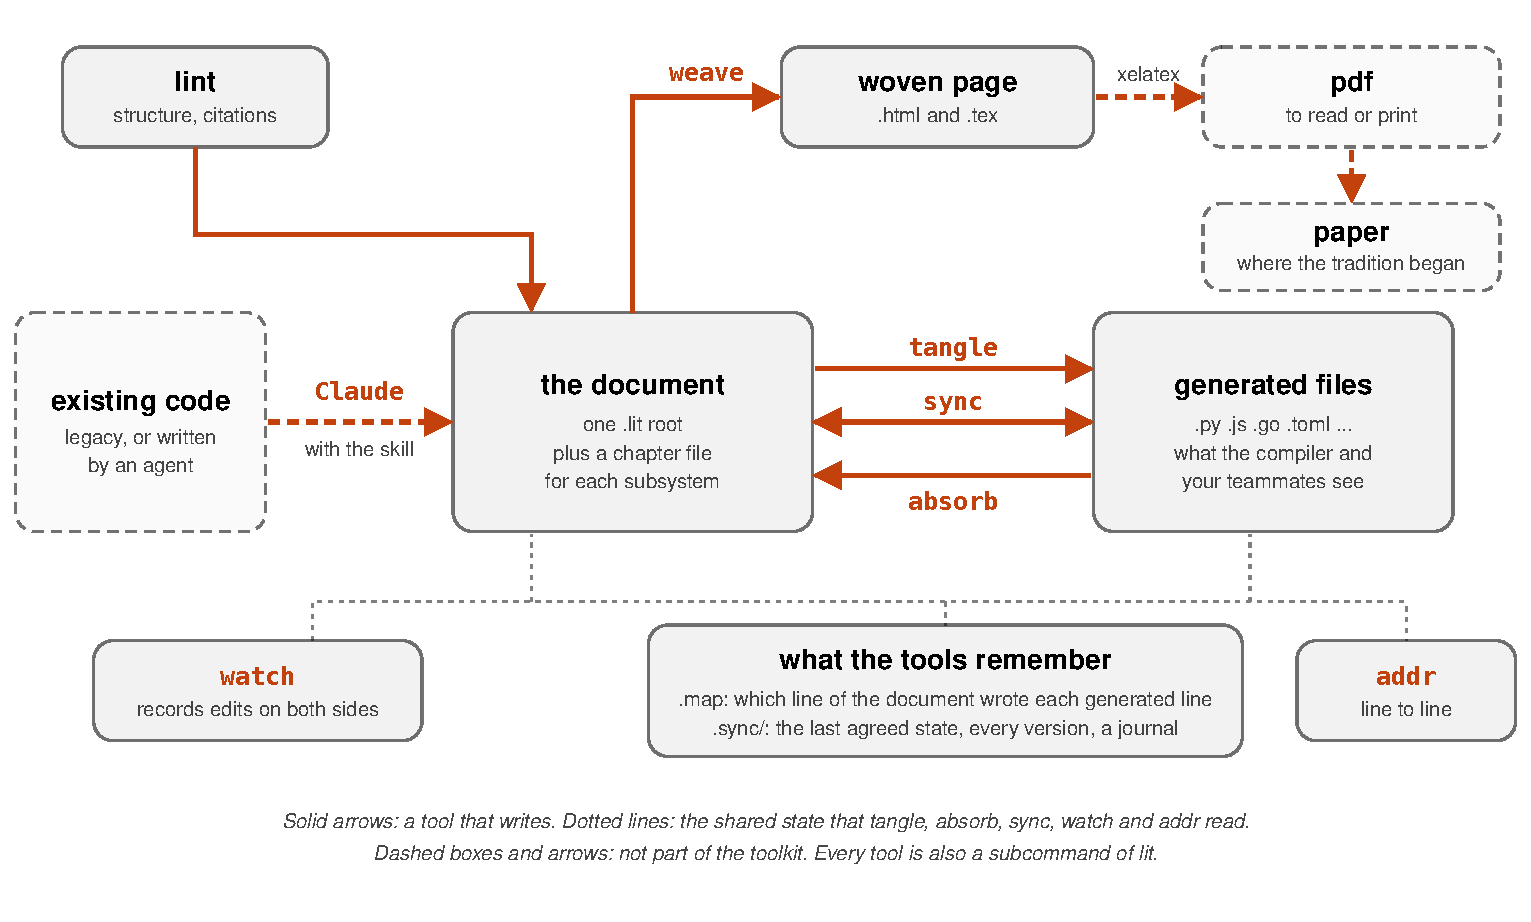
\includegraphics[width=\linewidth]{tools.pdf}
{\small\itshape The tools at a glance: weave reads the document; tangle, sync and absorb move text between it and the generated files; the map and the sync base are what let them agree.\par}
\end{figure}

\chunkhead{chunk1}{\filebadge\ \textbf{\texttt{internal/\allowbreak{}skill/\allowbreak{}files/\allowbreak{}docs/\allowbreak{}tools.\allowbreak{}svg}}}
The figure is a file chunk of this document, so it is tangled like code, and the woven HTML inlines it from here. It is plain SVG with the colours of the text, so it follows the page in light and dark and prints black on white. Every tool is a labelled arrow; the boxes are the places text lives.
\begin{Verbatim}
<svg xmlns="http://www.w3.org/2000/svg" viewBox="0 0 980 590" width="980" height="590">
  <title>How the tools move text between the literate document, the generated files and the woven page</title>
  <style>
    .fx-box \{ fill: currentColor; fill-opacity: .05; stroke: currentColor; stroke-opacity: .55; stroke-width: 1.5 \}
    .fx-out \{ stroke-dasharray: 7 5; fill-opacity: .02 \}
    .fx-t \{ font: 600 18px system-ui, Helvetica, Arial, sans-serif; fill: currentColor \}
    .fx-s \{ font: 13px system-ui, Helvetica, Arial, sans-serif; fill: currentColor; fill-opacity: .72 \}
    .fx-tool \{ font: 700 16px ui-monospace, Menlo, Consolas, monospace; fill: #c2410c \}
    .fx-arrow \{ stroke: #c2410c; stroke-width: 2.6; fill: none \}
    .fx-thin \{ stroke: currentColor; stroke-opacity: .5; stroke-width: 1.4; stroke-dasharray: 3 4; fill: none \}
    .fx-note \{ font: italic 13px system-ui, Helvetica, Arial, sans-serif; fill: currentColor; fill-opacity: .72 \}
  </style>
  <defs>
    <marker id="fx-r" viewBox="0 0 10 10" refX="9" refY="5" markerWidth="7" markerHeight="7" orient="auto">
      <path d="M0 0L10 5L0 10z" fill="#c2410c"/>
    </marker>
    <marker id="fx-l" viewBox="0 0 10 10" refX="1" refY="5" markerWidth="7" markerHeight="7" orient="auto">
      <path d="M10 0L0 5L10 10z" fill="#c2410c"/>
    </marker>
  </defs>

  <!-- the three places text lives -->
  <rect class="fx-box fx-out" x="10" y="200" width="160" height="140" rx="12"/>
  <text class="fx-t" x="90" y="262" text-anchor="middle">existing code</text>
  <text class="fx-s" x="90" y="284" text-anchor="middle">legacy, or written</text>
  <text class="fx-s" x="90" y="302" text-anchor="middle">by an agent</text>

  <rect class="fx-box" x="290" y="200" width="230" height="140" rx="12"/>
  <text class="fx-t" x="405" y="252" text-anchor="middle">the document</text>
  <text class="fx-s" x="405" y="276" text-anchor="middle">one .lit root</text>
  <text class="fx-s" x="405" y="294" text-anchor="middle">plus a chapter file</text>
  <text class="fx-s" x="405" y="312" text-anchor="middle">for each subsystem</text>

  <rect class="fx-box" x="700" y="200" width="230" height="140" rx="12"/>
  <text class="fx-t" x="815" y="252" text-anchor="middle">generated files</text>
  <text class="fx-s" x="815" y="276" text-anchor="middle">.py  .js  .go  .toml ...</text>
  <text class="fx-s" x="815" y="294" text-anchor="middle">what the compiler and</text>
  <text class="fx-s" x="815" y="312" text-anchor="middle">your teammates see</text>

  <!-- reading: lit -> woven -> pdf -->
  <rect class="fx-box" x="500" y="30" width="200" height="64" rx="12"/>
  <text class="fx-t" x="600" y="58" text-anchor="middle">woven page</text>
  <text class="fx-s" x="600" y="78" text-anchor="middle">.html and .tex</text>
  <rect class="fx-box fx-out" x="770" y="30" width="190" height="64" rx="12"/>
  <text class="fx-t" x="865" y="58" text-anchor="middle">pdf</text>
  <text class="fx-s" x="865" y="78" text-anchor="middle">to read or print</text>
  <path class="fx-arrow" d="M405 200 V62 H498" marker-end="url(#fx-r)"/>
  <text class="fx-tool" x="452" y="52" text-anchor="middle">weave</text>
  <path class="fx-arrow" d="M702 62 H768" marker-end="url(#fx-r)" stroke-dasharray="7 5"/>
  <text class="fx-s" x="735" y="52" text-anchor="middle">xelatex</text>
  <path class="fx-arrow" d="M865 96 V128" marker-end="url(#fx-r)" stroke-dasharray="7 5" stroke-width="1.8"/>
  <rect class="fx-box fx-out" x="770" y="130" width="190" height="56" rx="12"/>
  <text class="fx-t" x="865" y="154" text-anchor="middle">paper</text>
  <text class="fx-s" x="865" y="173" text-anchor="middle">where the tradition began</text>

  <!-- checking -->
  <rect class="fx-box" x="40" y="30" width="170" height="64" rx="12"/>
  <text class="fx-t" x="125" y="58" text-anchor="middle">lint</text>
  <text class="fx-s" x="125" y="78" text-anchor="middle">structure, citations</text>
  <path class="fx-arrow" d="M125 94 V150 H340 V198" marker-end="url(#fx-r)" stroke-width="1.8"/>

  <!-- writing: existing code -> lit -->
  <path class="fx-arrow" d="M172 270 H288" marker-end="url(#fx-r)" stroke-dasharray="7 5"/>
  <text class="fx-tool" x="230" y="256" text-anchor="middle">Claude</text>
  <text class="fx-s" x="230" y="292" text-anchor="middle">with the skill</text>

  <!-- the three ways between document and files -->
  <path class="fx-arrow" d="M522 236 H698" marker-end="url(#fx-r)"/>
  <text class="fx-tool" x="610" y="228" text-anchor="middle">tangle</text>
  <path class="fx-arrow" d="M522 270 H698" marker-start="url(#fx-l)" marker-end="url(#fx-r)"/>
  <text class="fx-tool" x="610" y="262" text-anchor="middle">sync</text>
  <path class="fx-arrow" d="M698 304 H522" marker-end="url(#fx-r)"/>
  <text class="fx-tool" x="610" y="326" text-anchor="middle">absorb</text>

  <!-- shared state -->
  <path class="fx-thin" d="M200 410 V385 H900 V410 M340 385 V342 M800 385 V342 M605 385 V400"/>
  <rect class="fx-box" x="415" y="400" width="380" height="84" rx="12"/>
  <text class="fx-t" x="605" y="428" text-anchor="middle">what the tools remember</text>
  <text class="fx-s" x="605" y="452" text-anchor="middle">.map: which line of the document wrote each generated line</text>
  <text class="fx-s" x="605" y="470" text-anchor="middle">.sync/: the last agreed state, every version, a journal</text>

  <rect class="fx-box" x="60" y="410" width="210" height="64" rx="12"/>
  <text class="fx-tool" x="165" y="438" text-anchor="middle">watch</text>
  <text class="fx-s" x="165" y="458" text-anchor="middle">records edits on both sides</text>
  <rect class="fx-box" x="830" y="410" width="140" height="64" rx="12"/>
  <text class="fx-tool" x="900" y="438" text-anchor="middle">addr</text>
  <text class="fx-s" x="900" y="458" text-anchor="middle">line to line</text>

  <text class="fx-note" x="490" y="530" text-anchor="middle">Solid arrows: a tool that writes. Dotted lines: the shared state that tangle, absorb, sync, watch and addr read.</text>
  <text class="fx-note" x="490" y="550" text-anchor="middle">Dashed boxes and arrows: not part of the toolkit. Every tool is also a subcommand of lit.</text>
</svg>
\end{Verbatim}

\hypertarget{h-Where-literate-programming-came-from-and-where-this-is-going}{}\phantomsection\addcontentsline{toc}{section}{Where literate programming came from, and where this is going}
\section*{Where literate programming came from, and where this is going}

Literate programming began as a way of writing a program to be read. In Knuth's account \cite{knuth1984lp} a program is a work of exposition: a web of parts, presented in the order that is best for a person, from which the order the machine needs is derived. As far as the author of this document knows, such programs were first worked out on paper, as a text for people, and only then entered into a computer, and Knuth's own programs are the model of the kind. The paper was the point; the computer was how the program got to run.

The tools that followed were, for the most part, made by and for people who write papers and books. They put the document first and treat a program as an illustration in it, and they are a poor fit for a team that maintains software which already exists, in a language and a repository it did not choose. Ramsey's simplification \cite{ramsey1994lp} removed the dependence on a language, and that is the line this toolkit follows. What it adds is for the working programmer: tools for the day somebody edits the generated code, for programs that are being converted and not written, and for gaps that an assistant can fill.

Notebooks are what most people meet today, and a notebook is not a literate program in the sense above. Its cells run in the order in which they are arranged, so the order of the explanation and the order of execution are one and the same, which is the constraint that literate programming exists to remove. There are no named parts that are defined in one place and used in another, nothing is tangled into the files of a program, and hidden state lets a notebook read well and still fail when it is run from the top. Notebooks are good for exploring data. They are a different thing, and this toolkit does not try to be one.

Two things follow for the shape of this document. The paper is a first-class output: weave writes LaTeX, so the program can be printed and read away from a screen, which is how a book should be read, and the document is written to be read from the first page. And the order of the chapters is the order of importance. The ideas come first, and then the tools, with the gap-filling assistant near the end of the story. What a reader could write for themselves, the plain details of the program, is at the bottom, in the appendix: the entry point, the argument parser, a text comparison, the installer, the license of the parser, the files of the skill, the landing page and the small helper functions that are named by their use.

\hypertarget{h-Reading-the-notation}{}\phantomsection\addcontentsline{toc}{section}{Reading the notation}
\section*{Reading the notation}

Everything starts with the grammar. A document is a tree of bags, written with a hash, a tag and braces. A bag whose tag is not reserved defines a chunk; the reserved tags are the headings, a citation, a bibliography, an include, an image and an agent hint. Code is any run of three or more backticks; shorter runs are inline code and belong to the prose. The parser is the brashtag package, compiled into the program, and a small wrapper gives it one more function, which parses a bag and returns the rest of the input.

Four rules make the text predictable. Chunk names are global, and defining a name twice concatenates the definitions, which is how a chunk can be explained in several places. A name that ends in an extension is a file. For programs too large for one file, \texttt{\#include\{chapter.\allowbreak{}lit\}} is replaced by the text of that file, so a program can have a chapter for each module or subsystem. And a bag called \texttt{agent-fill-in} inside a chunk is a gap: it is not code, tangle skips it, and \texttt{lit fill} knows how to fill it. All four rules are about the whole document, so no tool looks at a chunk in isolation, and a chunk in one chapter may refer to a chunk in another.

\hypertarget{h-Many-files-reading-a-program-from-pieces}{}\phantomsection\addcontentsline{toc}{section}{Many files: reading a program from pieces}
\section*{Many files: reading a program from pieces}

A program of any size is spread over several files, and the spread must not show in anything downstream. This chapter is how a root file and its chapters become one text.

\chunkhead{chunk2}{\textbf{\ensuremath{\langle}\texttt{source: pieces and the flat text}\ensuremath{\rangle}}\enspace\ensuremath{\equiv}}
\chunkmeta{used in \chunklink{chunk8}{\texttt{internal/\allowbreak{}lit/\allowbreak{}source.\allowbreak{}go}} \textperiodcentered{} part of \hyperref[chunk8]{\texttt{internal/\allowbreak{}lit/\allowbreak{}source.\allowbreak{}go}}}
A large program is split over files, and the split must not show in anything downstream. A \texttt{Source} is the root file with every \texttt{\#include\{chapter.\allowbreak{}lit\}} replaced by the text of that file, recursively and relative to the including file. What comes out is one flat text, which every other tool works on exactly as if it had been written in one file, and a table of pieces that says which stretch of the flat text came from which file at which offset.
\begin{Verbatim}
package lit

import (
	"fmt"
	"os"
	"path/filepath"
	"strings"
	"unicode/utf8"

	"github.com/pratikdeoghare/lit/internal/brashtag"
)

// A Piece says that Text[Start:End] came from file Name, starting at byte Ofs of that file.
type Piece struct \{
	Start, End int
	Name       string
	Ofs        int
\}

// Source is a literate program made of one or more files, seen as one text.
//
// "#include\{chapter.lit\}" anywhere in a file is replaced by the text of that file (relative to the including
// file), so every tool works on one flat text, Text, and Pieces remembers which stretch of it came from which
// file. Edits to the flat text are carried back to the files by SplitBack and WriteBack.
type Source struct \{
	Root   string            // the root file, as given
	Base   string            // its directory
	Texts  map[string]string // file name (relative to Base, slashes) -> its text
	Order  []string          // the files, root first, in the order they were read
	Pieces []Piece
	Text   string
\}

type reader func(path string) (string, error)

func diskReader(path string) (string, error) \{
	b, err := os.ReadFile(path)
	return string(b), err
\}

// ReadSource reads the root file and everything it includes.
func ReadSource(path string) (*Source, error) \{ return readSource(path, diskReader) \}
\end{Verbatim}

\chunkhead{chunk3}{\textbf{\ensuremath{\langle}\texttt{source: reading and expanding}\ensuremath{\rangle}}\enspace\ensuremath{\equiv}}
\chunkmeta{used in \chunklink{chunk8}{\texttt{internal/\allowbreak{}lit/\allowbreak{}source.\allowbreak{}go}} \textperiodcentered{} part of \hyperref[chunk8]{\texttt{internal/\allowbreak{}lit/\allowbreak{}source.\allowbreak{}go}}}
Reading starts at the root and expands includes depth first. A file that includes itself, directly or through another, is reported with the chain; a file included twice is reported too, because its chunks would be defined twice. Each file must be balanced on its own, so an error is blamed on the file it is in.
\begin{Verbatim}
func readSource(path string, read reader) (*Source, error) \{
	s := &Source\{Root: filepath.Clean(path), Texts: map[string]string\{\}\}
	s.Base = filepath.Dir(s.Root)
	var parts []part
	if err := s.expand(s.Root, nil, &parts, read); err != nil \{
		return nil, err
	\}
	var sb strings.Builder
	for _, p := range parts \{
		s.Pieces = append(s.Pieces, Piece\{sb.Len(), sb.Len() + len(p.text), p.name, p.ofs\})
		sb.WriteString(p.text)
	\}
	s.Text = sb.String()
	return s, nil
\}

type part struct \{
	text, name string
	ofs        int
\}

// Rel names a path of the program relative to the root's directory, with forward slashes.
func (s *Source) Rel(path string) string \{
	r, err := filepath.Rel(s.Base, path)
	if err != nil \{
		r = path
	\}
	return filepath.ToSlash(r)
\}

func (s *Source) expand(path string, stack []string, parts *[]part, read reader) error \{
	name := s.Rel(path)
	for _, p := range stack \{
		if p == path \{
			var names []string
			for _, q := range append(append([]string\{\}, stack...), path) \{
				names = append(names, s.Rel(q))
			\}
			return fmt.Errorf("recursive #include: %s", strings.Join(names, " -> "))
		\}
	\}
	if _, dup := s.Texts[name]; dup \{
		return fmt.Errorf("%s is included twice; each chapter file may appear once (use <<<chunk>>> references to share code)", name)
	\}
	text, err := read(path)
	if err != nil \{
		who := name
		if len(stack) > 0 \{
			who = s.Rel(stack[len(stack)-1])
		\}
		return fmt.Errorf("%s: cannot read %s: %v", who, path, unwrap(err))
	\}
	if strings.Contains(text, "\textbackslash{}r") \{
		return fmt.Errorf("%s: carriage returns found; convert it to LF line endings (the sourcemap uses offsets)", path)
	\}
	s.Texts[name] = text
	s.Order = append(s.Order, name)
	incs, err := includes(text, name)
	if err != nil \{
		return err
	\}
	at := 0
	for _, inc := range incs \{
		*parts = append(*parts, part\{text[at:inc.start], name, at\})
		sub := filepath.Clean(filepath.Join(filepath.Dir(path), inc.path))
		if _, err := read(sub); err != nil \{
			return fmt.Errorf("%s:%d: #include\{%s\}: no such file", name, inc.line, inc.path)
		\}
		if err := s.expand(sub, append(append([]string\{\}, stack...), path), parts, read); err != nil \{
			return err
		\}
		at = inc.end
	\}
	*parts = append(*parts, part\{text[at:], name, at\})
	return nil
\}

func unwrap(err error) string \{
	if pe, ok := err.(*os.PathError); ok \{
		return pe.Err.Error()
	\}
	return err.Error()
\}
\end{Verbatim}

\chunkhead{chunk4}{\textbf{\ensuremath{\langle}\texttt{source: finding the includes}\ensuremath{\rangle}}\enspace\ensuremath{\equiv}}
\chunkmeta{used in \chunklink{chunk8}{\texttt{internal/\allowbreak{}lit/\allowbreak{}source.\allowbreak{}go}} \textperiodcentered{} part of \hyperref[chunk8]{\texttt{internal/\allowbreak{}lit/\allowbreak{}source.\allowbreak{}go}}}
Includes are found in the parse tree, not with a regular expression, so one inside code or in the middle of a word is never mistaken for a directive. The tree is lossless, so walking it and adding up lengths gives the offset of every include bag.
\begin{Verbatim}
type include struct \{
	start, end int
	path       string
	line       int
\}

// includes finds the #include\{path\} bags of one file. They are found in the parse tree, not with a regular
// expression, so one inside code is never mistaken for a directive; the walk does not look inside them.
func includes(text, name string) ([]include, error) \{
	root, err := ParseText(text, func(off int) string \{
		return fmt.Sprintf("%s:%d", name, strings.Count(text[:min(off, len(text))], "\textbackslash{}n")+1)
	\})
	if err != nil \{
		return nil, err
	\}
	var found []include
	var bad error
	Walk(root, func(n brashtag.Node, parents []brashtag.Bag, start, end int) bool \{
		b, ok := n.(brashtag.Bag)
		if !ok || b.Tag() != "include" \{
			return true
		\}
		var sb strings.Builder
		for _, k := range b.Kids() \{
			bl, ok := k.(brashtag.Blob)
			if !ok \{
				bad = fmt.Errorf("%s:%d: #include\{\} wants a file name", name, strings.Count(text[:start], "\textbackslash{}n")+1)
				return false
			\}
			sb.WriteString(bl.Text())
		\}
		p := strings.TrimSpace(sb.String())
		if p == "" \{
			bad = fmt.Errorf("%s:%d: #include\{\} wants a file name", name, strings.Count(text[:start], "\textbackslash{}n")+1)
			return false
		\}
		found = append(found, include\{start, end, p, strings.Count(text[:start], "\textbackslash{}n") + 1\})
		return false
	\})
	return found, bad
\}

// ---- positions
\end{Verbatim}

\chunkhead{chunk5}{\textbf{\ensuremath{\langle}\texttt{source: positions}\ensuremath{\rangle}}\enspace\ensuremath{\equiv}}
\chunkmeta{used in \chunklink{chunk8}{\texttt{internal/\allowbreak{}lit/\allowbreak{}source.\allowbreak{}go}} \textperiodcentered{} part of \hyperref[chunk8]{\texttt{internal/\allowbreak{}lit/\allowbreak{}source.\allowbreak{}go}}}
Two functions turn positions around. \texttt{Locate} maps an offset in the flat text to a file, a line and a column, which is how every message and every address names the chapter and the line in it. \texttt{FlatOffset} goes the other way, and says no for a spot that is not part of the text, such as the line of an include directive.
\begin{Verbatim}
func (s *Source) piece(off int) Piece \{
	for _, p := range s.Pieces \{
		if p.Start <= off && off < p.End \{
			return p
		\}
	\}
	if n := len(s.Pieces); n > 0 \{
		return s.Pieces[n-1]
	\}
	return Piece\{Name: s.Rel(s.Root)\}
\}

// Locate maps an offset in the flat text to a file, a line and a column (both 1-based, columns in characters).
func (s *Source) Locate(off int) (name string, line, col int) \{
	p := s.piece(off)
	at := p.Ofs + (off - p.Start)
	text := s.Texts[p.Name]
	if at > len(text) \{
		at = len(text)
	\}
	line = strings.Count(text[:at], "\textbackslash{}n") + 1
	col = utf8.RuneCountInString(text[strings.LastIndex(text[:at], "\textbackslash{}n")+1:at]) + 1
	return p.Name, line, col
\}

// Where says "file:line" for an offset of the flat text.
func (s *Source) Where(off int) string \{
	n, l, _ := s.Locate(off)
	return fmt.Sprintf("%s:%d", n, l)
\}

// FlatOffset maps (file, line, column) to an offset of the flat text; ok is false if that spot is not part of it
// (the line of an #include directive, say).
func (s *Source) FlatOffset(name string, line, col int) (int, bool) \{
	text, known := s.Texts[name]
	if !known \{
		return 0, false
	\}
	at := 0
	for i, l := range strings.Split(text, "\textbackslash{}n") \{
		if i == line-1 \{
			break
		\}
		at += len(l) + 1
	\}
	at += col - 1
	for _, p := range s.Pieces \{
		if p.Name == name && p.Ofs <= at && at < p.Ofs+(p.End-p.Start) \{
			return p.Start + at - p.Ofs, true
		\}
	\}
	return 0, false
\}

// Parse parses the flat text.
func (s *Source) Parse() (brashtag.Bag, error) \{ return ParseText(s.Text, s.Where) \}

// ---- writing back
\end{Verbatim}

\chunkhead{chunk6}{\textbf{\ensuremath{\langle}\texttt{source: carrying edits back}\ensuremath{\rangle}}\enspace\ensuremath{\equiv}}
\chunkmeta{used in \chunklink{chunk8}{\texttt{internal/\allowbreak{}lit/\allowbreak{}source.\allowbreak{}go}} \textperiodcentered{} part of \hyperref[chunk8]{\texttt{internal/\allowbreak{}lit/\allowbreak{}source.\allowbreak{}go}}}
An edit of the flat text has to be carried back to the files. \texttt{SplitBack} finds the edits with a line diff, cuts each one at the seams between files, and returns the new text of just the files that changed. It then reads the result again and insists that it flattens to exactly the text it was given, so an edit that would add or move an include is refused rather than guessed. Text inserted exactly on a seam goes to the end of the earlier file.
\begin{Verbatim}
func splitKeep(s string) []string \{
	var out []string
	for len(s) > 0 \{
		i := strings.IndexByte(s, '\textbackslash{}n')
		if i < 0 \{
			out = append(out, s)
			break
		\}
		out = append(out, s[:i+1])
		s = s[i+1:]
	\}
	return out
\}

type edit struct \{
	a0, a1 int
	rep    string
\}

// SplitBack returns the new text of every file that changes when the flat text becomes newText. The edits are
// found with a line diff and cut at the seams between files; the result is read again and must flatten to
// exactly newText, so an edit that would add, remove or move an #include is refused rather than guessed.
// Text inserted exactly on a seam goes to the end of the earlier file.
func (s *Source) SplitBack(newText string) (map[string]string, error) \{
	old := s.Text
	if newText == old \{
		return nil, nil
	\}
	la, lb := splitKeep(old), splitKeep(newText)
	ca, cb := cum(la), cum(lb)
	var edits []edit
	for _, h := range Hunks(la, lb) \{
		a0, a1, rep := ca[h.A0], ca[h.A1], newText[cb[h.B0]:cb[h.B1]]
		straddle := false
		for _, p := range s.Pieces \{
			if a0 < p.Start && p.Start < a1 \{
				straddle = true
			\}
		\}
		if !straddle \{
			edits = append(edits, edit\{a0, a1, rep\})
			continue
		\}
		ra, rb := runes(old[a0:a1]), runes(rep)
		pa := cum(ra)
		for _, h2 := range Hunks(ra, rb) \{
			edits = append(edits, edit\{a0 + pa[h2.A0], a0 + pa[h2.A1], strings.Join(rb[h2.B0:h2.B1], "")\})
		\}
	\}
	per := map[string][]edit\{\}
	for _, e := range edits \{
		if e.a0 == e.a1 \{ // an insertion belongs to the file that ends there
			var pc *Piece
			for i := range s.Pieces \{
				if p := &s.Pieces[i]; p.Start < e.a0 && e.a0 <= p.End \{
					pc = p
					break
				\}
			\}
			if pc == nil \{
				for i := range s.Pieces \{
					if p := &s.Pieces[i]; p.Start == e.a0 \{
						pc = p
						break
					\}
				\}
			\}
			per[pc.Name] = append(per[pc.Name], edit\{pc.Ofs + e.a0 - pc.Start, pc.Ofs + e.a0 - pc.Start, e.rep\})
			continue
		\}
		first := true
		for _, p := range s.Pieces \{
			lo, hi := max(e.a0, p.Start), min(e.a1, p.End)
			if lo < hi \{
				rep := ""
				if first \{
					rep = e.rep
				\}
				per[p.Name] = append(per[p.Name], edit\{p.Ofs + lo - p.Start, p.Ofs + hi - p.Start, rep\})
				first = false
			\}
		\}
	\}
	changed := map[string]string\{\}
	for name, eds := range per \{
		text, shift := s.Texts[name], 0
		sortEdits(eds)
		for _, e := range eds \{
			text = text[:e.a0+shift] + e.rep + text[e.a1+shift:]
			shift += len(e.rep) - (e.a1 - e.a0)
		\}
		changed[name] = text
	\}
	check, err := readSource(s.Root, func(path string) (string, error) \{
		if t, ok := changed[s.Rel(path)]; ok \{
			return t, nil
		\}
		return diskReaderOr(s, path)
	\})
	if err != nil || check.Text != newText \{
		return nil, fmt.Errorf("the edit cannot be carried back to the chapter files (it adds, removes or moves an #include); change the #include lines in the files themselves")
	\}
	return changed, nil
\}

func diskReaderOr(s *Source, path string) (string, error) \{
	if t, ok := s.Texts[s.Rel(path)]; ok \{
		return t, nil
	\}
	return diskReader(path)
\}

func sortEdits(e []edit) \{
	for i := 1; i < len(e); i++ \{
		for j := i; j > 0 && (e[j].a0 < e[j-1].a0 || (e[j].a0 == e[j-1].a0 && e[j].a1 < e[j-1].a1)); j-- \{
			e[j], e[j-1] = e[j-1], e[j]
		\}
	\}
\}

func cum(parts []string) []int \{
	out := make([]int, len(parts)+1)
	for i, p := range parts \{
		out[i+1] = out[i] + len(p)
	\}
	return out
\}

func runes(s string) []string \{
	var out []string
	for _, r := range s \{
		out = append(out, string(r))
	\}
	return out
\}
\end{Verbatim}

\chunkhead{chunk7}{\textbf{\ensuremath{\langle}\texttt{source: writing the files}\ensuremath{\rangle}}\enspace\ensuremath{\equiv}}
\chunkmeta{used in \chunklink{chunk8}{\texttt{internal/\allowbreak{}lit/\allowbreak{}source.\allowbreak{}go}} \textperiodcentered{} part of \hyperref[chunk8]{\texttt{internal/\allowbreak{}lit/\allowbreak{}source.\allowbreak{}go}}}
Writing goes through a temporary file and a rename, so a crash cannot leave a half-written chapter.
\begin{Verbatim}
// WriteBack writes the files that change when the flat text becomes newText and returns old and new text of each.
func (s *Source) WriteBack(newText string) (map[string][2]string, error) \{
	changed, err := s.SplitBack(newText)
	if err != nil \{
		return nil, err
	\}
	done := map[string][2]string\{\}
	for name, text := range changed \{
		path := filepath.Join(s.Base, filepath.FromSlash(name))
		tmp := path + ".lit.tmp"
		if err := os.WriteFile(tmp, []byte(text), 0o644); err != nil \{
			return nil, err
		\}
		if err := os.Rename(tmp, path); err != nil \{
			return nil, err
		\}
		done[name] = [2]string\{s.Texts[name], text\}
	\}
	n, err := ReadSource(s.Root)
	if err != nil \{
		return nil, err
	\}
	*s = *n
	return done, nil
\}
\end{Verbatim}

\chunkhead{chunk8}{\filebadge\ \textbf{\texttt{internal/\allowbreak{}lit/\allowbreak{}source.\allowbreak{}go}}}
The file is its parts, in the order of the source.
\begin{Verbatim}
\chunkrefv{chunk2}

\chunkrefv{chunk3}

\chunkrefv{chunk4}

\chunkrefv{chunk5}

\chunkrefv{chunk6}

\chunkrefv{chunk7}
\end{Verbatim}

\hypertarget{h-Reading-the-notation-tangle}{}\phantomsection\addcontentsline{toc}{section}{Reading the notation: tangle}
\section*{Reading the notation: tangle}

Tangle is the foundation and the smallest tool: it turns a document into files. Every other tool uses it, because the definition of the notation lives here and nowhere else.

\chunkhead{chunk9}{\textbf{\ensuremath{\langle}\texttt{tangle: the grammar's constants}\ensuremath{\rangle}}\enspace\ensuremath{\equiv}}
\chunkmeta{used in \chunklink{chunk19}{\texttt{internal/\allowbreak{}lit/\allowbreak{}tangle.\allowbreak{}go}} \textperiodcentered{} part of \hyperref[chunk19]{\texttt{internal/\allowbreak{}lit/\allowbreak{}tangle.\allowbreak{}go}}}
The tangle file holds the definition of the notation, and every other file depends on it. Three small regular expressions carry most of it. A reference is a line of nothing but \texttt{\textless{}\textless{}\textless{}name\textgreater{}\textgreater{}\textgreater{}}, the escaped form is the same line with a backslash in front, and a file is a chunk whose name ends in an extension. The escape exists because a document about this notation has to be able to contain a reference line that is not one: the backslash is removed on the way out and nothing else changes. The reserved tags are a set, with the hint tag among them.
\begin{Verbatim}
package lit

import (
	"fmt"
	"os"
	"path/filepath"
	"regexp"
	"strings"

	"github.com/pratikdeoghare/lit/internal/brashtag"
)

type (
	Bag  = brashtag.Bag
	Blob = brashtag.Blob
	Code = brashtag.Code
	Node = brashtag.Node
)

// Reserved tags: they are never chunks. Everything else that is a bag defines a chunk.
var Reserved = map[string]bool\{
	"h1": true, "h2": true, "h3": true, "h4": true, "h5": true, "h6": true,
	"cite": true, "bibliography": true, "include": true, "img": true, "agent-fill-in": true,
\}

const HintTag = "agent-fill-in"

var (
	refRe     = regexp.MustCompile(`^(\textbackslash{}s*)<<<(.+?)>>>\textbackslash{}s*$`)
	escapedRe = regexp.MustCompile(`^(\textbackslash{}s*)\textbackslash{}\textbackslash{}(\textbackslash{}\textbackslash{}*<<<.+?>>>\textbackslash{}s*)$`)
	fileRe    = regexp.MustCompile(`\textbackslash{}.\textbackslash{}w+$`)
)

func isHeading(tag string) bool \{
	return len(tag) == 2 && tag[0] == 'h' && tag[1] >= '1' && tag[1] <= '6'
\}

// ---- walking the tree with positions
\end{Verbatim}

\chunkhead{chunk10}{\textbf{\ensuremath{\langle}\texttt{tangle: walking with positions}\ensuremath{\rangle}}\enspace\ensuremath{\equiv}}
\chunkmeta{used in \chunklink{chunk19}{\texttt{internal/\allowbreak{}lit/\allowbreak{}tangle.\allowbreak{}go}} \textperiodcentered{} part of \hyperref[chunk19]{\texttt{internal/\allowbreak{}lit/\allowbreak{}tangle.\allowbreak{}go}}}
The parser reports no positions, but its tree is lossless, so a walk that adds up lengths gives the byte offset of every node. The visitor can decline to descend into a bag, and is told which bags enclose the node.
\begin{Verbatim}
// Walk visits every node with its byte offsets [start,end) in the text the tree was parsed from (the text
// inside the implicit root). The tree is lossless, so offsets come from adding up lengths. f returns false
// to skip the children of a bag. parents ends with the bag that holds the node.
func Walk(root Bag, f func(n Node, parents []Bag, start, end int) bool) \{
	pos := 0
	var rec func(b Bag, parents []Bag)
	rec = func(b Bag, parents []Bag) \{
		ps := append(append([]Bag\{\}, parents...), b)
		for _, k := range b.Kids() \{
			switch k := k.(type) \{
			case Blob:
				start := pos
				pos += len(k.Text())
				f(k, ps, start, pos)
			case Code:
				start := pos
				pos += 2*len(k.Tag()) + len(k.Text())
				f(k, ps, start, pos)
			case Bag:
				start := pos
				inner := innerLen(k)
				pos = start + len(k.Tag()) + 2
				if f(k, ps, start, start+len(k.Tag())+2+inner+1) \{
					rec(k, ps)
				\} else \{
					pos += inner
				\}
				pos++ // the closing brace
			\}
		\}
	\}
	rec(root, nil)
\}

func innerLen(b Bag) int \{
	n := 0
	for _, k := range b.Kids() \{
		switch k := k.(type) \{
		case Blob:
			n += len(k.Text())
		case Code:
			n += 2*len(k.Tag()) + len(k.Text())
		case Bag:
			n += len(k.Tag()) + 2 + innerLen(k) + 1
		\}
	\}
	return n
\}

// ---- parsing
\end{Verbatim}

\chunkhead{chunk11}{\textbf{\ensuremath{\langle}\texttt{tangle: parsing a document}\ensuremath{\rangle}}\enspace\ensuremath{\equiv}}
\chunkmeta{used in \chunklink{chunk19}{\texttt{internal/\allowbreak{}lit/\allowbreak{}tangle.\allowbreak{}go}} \textperiodcentered{} part of \hyperref[chunk19]{\texttt{internal/\allowbreak{}lit/\allowbreak{}tangle.\allowbreak{}go}}}
The parser reads only the first bag of its input and would silently ignore the rest of a file, so the text is wrapped in an implicit root bag. The text it consumed has to equal the text it was given, which catches a stray closing brace; a stray hash becomes a tag that no sensible chunk name could be, and is reported with a file and a line, taken from the flat text through a callback.
\begin{Verbatim}
// ParseText parses literate text into a root bag. where(offset) names a position in the text for messages.
func ParseText(text string, where func(int) string) (Bag, error) \{
	const head = "#document\{"
	root, rest, err := brashtag.ParseRest(head + text + "\}")
	at := func(r string) int \{ return max(0, len(text)+1-len(r)) \}
	if err != nil \{
		off := at(rest)
		msg := err.Error()
		if strings.HasPrefix(msg, "unexpected \{") \{
			if i := strings.IndexByte(rest, '\{'); i >= 0 \{
				off = at(rest) + i
			\}
			msg = "a \{ in prose. Put it inside backticks (a literal # \{ \} or tick outside code is not allowed)"
		\} else if rest == "" \{
			off = len(text)
		\}
		return Bag\{\}, fmt.Errorf("%s: %s", where(min(off, len(text))), msg)
	\}
	if strings.TrimSpace(rest) != "" \{
		off := at(rest) - 1
		snip := text[min(off, len(text)):]
		if len(snip) > 50 \{
			snip = snip[:50]
		\}
		return Bag\{\}, fmt.Errorf("%s: a stray '\}' in prose closed the document early, near: %q  (a literal '\}' or '#' outside backticks is not allowed)",
			where(min(off, len(text))), strings.TrimSpace(snip))
	\}
	var bad error
	var check func(b Bag)
	check = func(b Bag) \{
		t := b.Tag()
		if strings.Contains(t, "\textbackslash{}n") || strings.Contains(t, "#") || t != strings.TrimLeft(t, " \textbackslash{}t\textbackslash{}r\textbackslash{}n") || len(t) > 120 \{
			i := strings.Index(text, "#"+t[:min(30, len(t))])
			if bad == nil \{
				bad = fmt.Errorf("%s: suspicious bag tag %q...: a stray '#' in prose? (use backticks)", where(max(i, 0)), t[:min(40, len(t))])
			\}
		\}
		for _, k := range b.Kids() \{
			if kb, ok := k.(Bag); ok \{
				check(kb)
			\}
		\}
	\}
	check(root)
	if bad != nil \{
		return Bag\{\}, bad
	\}
	return root, nil
\}

// ParseFlat parses program text that is already spliced together (what Source.Text holds).
func ParseFlat(text string) (Bag, error) \{
	return ParseText(text, func(off int) string \{
		return fmt.Sprintf("program text line %d", strings.Count(text[:min(off, len(text))], "\textbackslash{}n")+1)
	\})
\}

// Load parses a .lit file and the chapter files it includes.
func Load(path string) (Bag, error) \{
	s, err := ReadSource(path)
	if err != nil \{
		return Bag\{\}, err
	\}
	return s.Parse()
\}

// ---- chunks
\end{Verbatim}

\chunkhead{chunk12}{\textbf{\ensuremath{\langle}\texttt{tangle: what is code}\ensuremath{\rangle}}\enspace\ensuremath{\equiv}}
\chunkmeta{used in \chunklink{chunk19}{\texttt{internal/\allowbreak{}lit/\allowbreak{}tangle.\allowbreak{}go}} \textperiodcentered{} part of \hyperref[chunk19]{\texttt{internal/\allowbreak{}lit/\allowbreak{}tangle.\allowbreak{}go}}}
A fence is a code run of three or more backticks. Its text is the lines between the fences, dedented by the indentation of the closing fence, which lets the author indent code to match the prose around it.
\begin{Verbatim}
func isFence(c Code) bool \{ return len(c.Tag()) >= 3 \}

// FenceText gives the lines of a fenced block: the newline after the opening fence is dropped, and the lines
// are dedented by the whitespace that precedes the closing fence.
func FenceText(c Code) []string \{
	lines := strings.Split(c.Text(), "\textbackslash{}n")
	if len(lines) > 0 && strings.TrimSpace(lines[0]) == "" \{
		lines = lines[1:]
	\}
	indent := ""
	if n := len(lines); n > 0 && strings.TrimSpace(lines[n-1]) == "" \{
		indent, lines = lines[n-1], lines[:n-1]
	\}
	out := make([]string, len(lines))
	for i, l := range lines \{
		if strings.HasPrefix(l, indent) \{
			out[i] = l[len(indent):]
		\} else \{
			out[i] = strings.TrimLeft(l, " \textbackslash{}t")
		\}
	\}
	return out
\}
\end{Verbatim}

\chunkhead{chunk13}{\textbf{\ensuremath{\langle}\texttt{tangle: collecting chunks}\ensuremath{\rangle}}\enspace\ensuremath{\equiv}}
\chunkmeta{used in \chunklink{chunk19}{\texttt{internal/\allowbreak{}lit/\allowbreak{}tangle.\allowbreak{}go}} \textperiodcentered{} part of \hyperref[chunk19]{\texttt{internal/\allowbreak{}lit/\allowbreak{}tangle.\allowbreak{}go}}}
Collection is one walk over the tree. Each fence is appended to its innermost chunk, in document order, so a chunk defined twice is the concatenation of both definitions. A hint is recorded as a hole, and when holes are asked for, a marker line is left in the chunk's code at that place, so that expansion carries the indentation and the place can be found again in the tangled text.
\begin{Verbatim}
// Chunks holds the code lines of every chunk (all fenced blocks of every definition, in document order).
type Chunks struct \{
	Order    []string
	Lines    map[string][]string
	Warnings []string
	Holes    []Hole
\}

// A Hole is an #agent-fill-in\{\} hint found inside a chunk. When holes are asked for, Collect leaves a marker
// line (see HoleMarker) where the hint was, so that expansion carries its indentation.
type Hole struct \{
	Index int
	Chunk string
	Bag   Bag
	Text  string // the hint, as plain text
\}

func HoleMarker(i int) string \{ return fmt.Sprintf("\textbackslash{}x00hole:%d", i) \}

var holeRe = regexp.MustCompile("^\textbackslash{}\textbackslash{}s*\textbackslash{}x00hole:(\textbackslash{}\textbackslash{}d+)$")

// Collect gathers the chunks of a document. With holes true, hints are recorded and marked in the code.
func Collect(root Bag, holes bool) *Chunks \{
	c := &Chunks\{Lines: map[string][]string\{\}\}
	var visit func(b Bag)
	visit = func(b Bag) \{
		name := strings.TrimSpace(b.Tag())
		if Reserved[name] \{
			return
		\}
		if _, ok := c.Lines[name]; !ok \{
			c.Order = append(c.Order, name)
			c.Lines[name] = nil
		\}
		for _, k := range b.Kids() \{
			switch k := k.(type) \{
			case Code:
				if isFence(k) \{
					c.Lines[name] = append(c.Lines[name], FenceText(k)...)
				\}
			case Bag:
				if k.Tag() == HintTag \{
					if holes \{
						h := Hole\{Index: len(c.Holes), Chunk: name, Bag: k, Text: PlainText(k)\}
						c.Holes = append(c.Holes, h)
						c.Lines[name] = append(c.Lines[name], HoleMarker(h.Index))
					\}
					continue
				\}
				visit(k)
			\}
		\}
	\}
	for _, k := range root.Kids() \{
		switch k := k.(type) \{
		case Code:
			if isFence(k) \{
				c.Warnings = append(c.Warnings, "code outside any chunk is ignored")
			\}
		case Bag:
			visit(k)
		\}
	\}
	return c
\}
\end{Verbatim}

\chunkhead{chunk14}{\textbf{\ensuremath{\langle}\texttt{tangle: text of a bag}\ensuremath{\rangle}}\enspace\ensuremath{\equiv}}
\chunkmeta{used in \chunklink{chunk19}{\texttt{internal/\allowbreak{}lit/\allowbreak{}tangle.\allowbreak{}go}} \textperiodcentered{} part of \hyperref[chunk19]{\texttt{internal/\allowbreak{}lit/\allowbreak{}tangle.\allowbreak{}go}}}
A bag's blobs and code spans as one line of text, for hints and messages.
\begin{Verbatim}
// PlainText is the text of a bag's blobs and code, with runs of white space made single spaces.
func PlainText(b Bag) string \{
	var sb strings.Builder
	for _, k := range b.Kids() \{
		switch k := k.(type) \{
		case Blob:
			sb.WriteString(k.Text())
		case Code:
			sb.WriteString(k.Text())
		\}
	\}
	return strings.Join(strings.Fields(sb.String()), " ")
\}

// Unescape is the text tangle writes for a code line: an escaped reference line loses its first backslash.
func Unescape(line string) string \{
	if m := escapedRe.FindStringSubmatch(line); m != nil \{
		return m[1] + m[2]
	\}
	return line
\}
\end{Verbatim}

\chunkhead{chunk15}{\textbf{\ensuremath{\langle}\texttt{tangle: expanding references}\ensuremath{\rangle}}\enspace\ensuremath{\equiv}}
\chunkmeta{used in \chunklink{chunk19}{\texttt{internal/\allowbreak{}lit/\allowbreak{}tangle.\allowbreak{}go}} \textperiodcentered{} part of \hyperref[chunk19]{\texttt{internal/\allowbreak{}lit/\allowbreak{}tangle.\allowbreak{}go}}}
Expansion is a recursion with an indentation: a reference alone on a line is replaced by the lines of its chunk, each shifted by the reference's own indentation. Writing \$E(c)\$ for the lines of chunk \$c\$, a line is either text, copied after removing one escape backslash, or a reference to \$r\$ at indentation \$i\$, which becomes \$i\$ prefixed to every non-blank line of \$E(r)\$. A chunk that reaches itself is reported with the path, rather than expanded forever.
\begin{Verbatim}
// Expand returns the lines of chunk name with every reference replaced by the lines of its chunk, indented
// by the reference's own indentation.
func (c *Chunks) Expand(name string) ([]string, error) \{ return c.expand(name, nil) \}

func (c *Chunks) expand(name string, trail []string) ([]string, error) \{
	lines, ok := c.Lines[name]
	if !ok \{
		return nil, fmt.Errorf("undefined chunk <<<%s>>>", name)
	\}
	for _, t := range trail \{
		if t == name \{
			return nil, fmt.Errorf("recursive chunk: %s", strings.Join(append(append([]string\{\}, trail...), name), " -> "))
		\}
	\}
	var out []string
	for _, line := range lines \{
		if m := refRe.FindStringSubmatch(line); m != nil \{
			sub, err := c.expand(strings.TrimSpace(m[2]), append(append([]string\{\}, trail...), name))
			if err != nil \{
				return nil, err
			\}
			for _, s := range sub \{
				if s != "" \{
					s = m[1] + s
				\}
				out = append(out, s)
			\}
		\} else if holeRe.MatchString(line) \{
			out = append(out, line)
		\} else \{
			out = append(out, Unescape(line))
		\}
	\}
	return out, nil
\}
\end{Verbatim}

\chunkhead{chunk16}{\textbf{\ensuremath{\langle}\texttt{tangle: files and what is used}\ensuremath{\rangle}}\enspace\ensuremath{\equiv}}
\chunkmeta{used in \chunklink{chunk19}{\texttt{internal/\allowbreak{}lit/\allowbreak{}tangle.\allowbreak{}go}} \textperiodcentered{} part of \hyperref[chunk19]{\texttt{internal/\allowbreak{}lit/\allowbreak{}tangle.\allowbreak{}go}}}
The files are the chunks whose names end in an extension, in the order they were first defined, and the used chunks are those that some code line references. A file's body ends with exactly one newline.
\begin{Verbatim}
// FileNames are the chunks that are written out as files, in the order they were first defined.
func (c *Chunks) FileNames() []string \{
	var out []string
	for _, n := range c.Order \{
		if fileRe.MatchString(n) \{
			out = append(out, n)
		\}
	\}
	return out
\}

// FileBody is what tangle writes for a file made of these lines.
func FileBody(lines []string) string \{
	body := strings.Join(lines, "\textbackslash{}n")
	if body == "" \{
		return ""
	\}
	return body + "\textbackslash{}n"
\}

// Used returns the names of the chunks that some code line references.
func (c *Chunks) Used() map[string]bool \{
	used := map[string]bool\{\}
	for _, lines := range c.Lines \{
		for _, l := range lines \{
			if m := refRe.FindStringSubmatch(l); m != nil \{
				used[strings.TrimSpace(m[2])] = true
			\}
		\}
	\}
	return used
\}
\end{Verbatim}

\chunkhead{chunk17}{\textbf{\ensuremath{\langle}\texttt{tangle: in memory}\ensuremath{\rangle}}\enspace\ensuremath{\equiv}}
\chunkmeta{used in \chunklink{chunk19}{\texttt{internal/\allowbreak{}lit/\allowbreak{}tangle.\allowbreak{}go}} \textperiodcentered{} part of \hyperref[chunk19]{\texttt{internal/\allowbreak{}lit/\allowbreak{}tangle.\allowbreak{}go}}}
Everything that needs the generated text without the disk, absorb, sync, the watcher and the checks, calls this: program text in, files out, in definition order.
\begin{Verbatim}
// TangleText tangles program text given as a string: \{file: generated text\}, in definition order.
func TangleText(text string) (map[string]string, []string, error) \{
	root, err := ParseFlat(text)
	if err != nil \{
		return nil, nil, err
	\}
	c := Collect(root, false)
	out := map[string]string\{\}
	var order []string
	for _, n := range c.FileNames() \{
		lines, err := c.Expand(n)
		if err != nil \{
			return nil, nil, err
		\}
		out[n] = FileBody(lines)
		order = append(order, n)
	\}
	return out, order, nil
\}

// ---- the command
\end{Verbatim}

\chunkhead{chunk18}{\textbf{\ensuremath{\langle}\texttt{tangle: the command}\ensuremath{\rangle}}\enspace\ensuremath{\equiv}}
\chunkmeta{used in \chunklink{chunk19}{\texttt{internal/\allowbreak{}lit/\allowbreak{}tangle.\allowbreak{}go}} \textperiodcentered{} part of \hyperref[chunk19]{\texttt{internal/\allowbreak{}lit/\allowbreak{}tangle.\allowbreak{}go}}}
The command writes every file chunk, warns about chunks that are never used and about hints still open, and then writes the sourcemap. Before it overwrites a file it hands the old and new text to the sync library, which keeps a copy of any edit that is about to be lost.
\begin{Verbatim}
const tangleUsage = "usage: lit tangle SOURCE.lit [OUTDIR] [--no-map]"

func Tangle(argv []string, io IO) int \{
	a, err := ParseArgs(argv, Spec\{Opts: map[string]bool\{"no-map": false\}\})
	if err != nil || len(a.Pos) == 0 || len(a.Pos) > 2 \{
		fmt.Fprintln(io.Err, tangleUsage)
		return 2
	\}
	srcPath, outdir := a.Pos[0], "."
	if len(a.Pos) > 1 \{
		outdir = a.Pos[1]
	\}
	src, err := ReadSource(srcPath)
	if err != nil \{
		fmt.Fprintln(io.Err, err)
		return 1
	\}
	root, err := src.Parse()
	if err != nil \{
		fmt.Fprintln(io.Err, err)
		return 1
	\}
	chunks := Collect(root, true)
	for _, w := range chunks.Warnings \{
		fmt.Fprintln(io.Err, "warning: "+w)
	\}
	used := chunks.Used()
	for _, n := range chunks.Order \{
		if !fileRe.MatchString(n) && !used[n] && len(chunks.Lines[n]) > 0 \{
			fmt.Fprintf(io.Err, "warning: chunk '%s' is never used\textbackslash{}n", n)
		\}
	\}
	if len(chunks.Holes) > 0 \{
		fmt.Fprintf(io.Err, "note: %d #%s hint(s) are still unfilled; the code they stand for is missing from the output (lit fill)\textbackslash{}n", len(chunks.Holes), HintTag)
	\}
	files := map[string]string\{\}
	for _, n := range chunks.FileNames() \{
		lines, err := chunks.Expand(n)
		if err != nil \{
			fmt.Fprintln(io.Err, err)
			return 1
		\}
		files[n] = FileBody(withoutHoles(lines))
	\}
	for _, n := range chunks.FileNames() \{
		path := filepath.Join(outdir, filepath.FromSlash(n))
		if err := os.MkdirAll(filepath.Dir(path), 0o755); err != nil \{
			fmt.Fprintln(io.Err, err)
			return 1
		\}
		protect(srcPath, outdir, n, path, files[n])
		if err := os.WriteFile(path, []byte(files[n]), 0o644); err != nil \{
			fmt.Fprintln(io.Err, err)
			return 1
		\}
		fmt.Fprintln(io.Out, "wrote", path)
	\}
	if !a.Has("no-map") \{
		p, err := WriteMap(srcPath, outdir)
		if err != nil \{
			fmt.Fprintf(io.Err, "note: no sourcemap written: %v\textbackslash{}n", err)
		\} else \{
			fmt.Fprintln(io.Out, "wrote", p)
		\}
	\}
	return 0
\}

func withoutHoles(lines []string) []string \{
	var out []string
	for _, l := range lines \{
		if !holeRe.MatchString(l) \{
			out = append(out, l)
		\}
	\}
	return out
\}
\end{Verbatim}

\chunkhead{chunk19}{\filebadge\ \textbf{\texttt{internal/\allowbreak{}lit/\allowbreak{}tangle.\allowbreak{}go}}}
The file is its parts, in the order of the source.
\begin{Verbatim}
\chunkrefv{chunk9}

\chunkrefv{chunk10}

\chunkrefv{chunk11}

\chunkrefv{chunk12}

\chunkrefv{chunk13}

\chunkrefv{chunk14}

\chunkrefv{chunk15}

\chunkrefv{chunk16}

\chunkrefv{chunk17}

\chunkrefv{chunk18}
\end{Verbatim}

\hypertarget{h-Positions-the-sourcemap}{}\phantomsection\addcontentsline{toc}{section}{Positions: the sourcemap}
\section*{Positions: the sourcemap}

The sourcemap is what makes a literate program editable from both ends. It records, for every generated line, the document line that produced it and the indentation that references added.

\chunkhead{chunk20}{\textbf{\ensuremath{\langle}\texttt{sourcemap: types}\ensuremath{\rangle}}\enspace\ensuremath{\equiv}}
\chunkmeta{used in \chunklink{chunk26}{\texttt{internal/\allowbreak{}lit/\allowbreak{}sourcemap.\allowbreak{}go}} \textperiodcentered{} part of \hyperref[chunk26]{\texttt{internal/\allowbreak{}lit/\allowbreak{}sourcemap.\allowbreak{}go}}}
The map speaks in character offsets of the flat text. A block is one fenced block of code: its chunk, its indentation and the offset of each of its lines. A segment says that a run of generated lines comes from a run of lines of a block, each with the indentation that references added in front. A segment is written as a JSON array of five numbers and a string, which keeps the map small and diffable.
\begin{Verbatim}
package lit

import (
	"bytes"
	"crypto/sha256"
	"encoding/hex"
	"encoding/json"
	"fmt"
	"os"
	"path/filepath"
	"strings"
)

const mapVersion = 1
const mark = "\textbackslash{}x00"

func sha256hex(s string) string \{
	h := sha256.Sum256([]byte(s))
	return hex.EncodeToString(h[:])
\}

// A Block is one fenced block of code in the program text: the chunk it belongs to, the indentation that was
// stripped from every line, the byte offsets [start,end) of each content line (end is before the newline),
// and whether a newline follows the last content line.
type Block struct \{
	Chunk  string   `json:"chunk"`
	Indent string   `json:"indent"`
	Lines  [][2]int `json:"lines"`
	NlLast bool     `json:"nl_last"`
\}

// A Seg says that generated lines At..At+N-1 (1-based) come from lines Line..Line+N-1 of block Block, each with
// Prefix (the indentation added by references) in front.
type Seg struct \{
	At, N, Block, Line int
	Prefix             string
\}

func (s Seg) MarshalJSON() ([]byte, error) \{
	return json.Marshal([]any\{s.At, s.N, s.Block, s.Line, s.Prefix\})
\}

func (s *Seg) UnmarshalJSON(b []byte) error \{
	var a [5]json.RawMessage
	if err := json.Unmarshal(b, &a); err != nil \{
		return err
	\}
	for i, p := range []*int\{&s.At, &s.N, &s.Block, &s.Line\} \{
		if err := json.Unmarshal(a[i], p); err != nil \{
			return err
		\}
	\}
	return json.Unmarshal(a[4], &s.Prefix)
\}

type FileEntry struct \{
	Sha256   string `json:"sha256"`
	Lines    int    `json:"lines"`
	Segments []Seg  `json:"segments"`
\}

// Map is the sourcemap: for every generated line, the line of the program that produced it.
type Map struct \{
	Version      int                  `json:"version"`
	Source       string               `json:"source"`
	Sources      []string             `json:"sources"`
	SourceSha256 string               `json:"source_sha256"`
	Blocks       []Block              `json:"blocks"`
	Files        map[string]FileEntry `json:"files"`
	FileOrder    []string             `json:"-"`
\}
\end{Verbatim}

\chunkhead{chunk21}{\textbf{\ensuremath{\langle}\texttt{sourcemap: building the map}\ensuremath{\rangle}}\enspace\ensuremath{\equiv}}
\chunkmeta{used in \chunklink{chunk26}{\texttt{internal/\allowbreak{}lit/\allowbreak{}sourcemap.\allowbreak{}go}} \textperiodcentered{} part of \hyperref[chunk26]{\texttt{internal/\allowbreak{}lit/\allowbreak{}sourcemap.\allowbreak{}go}}}
To learn which source line produced which generated line, every code line is tagged with an invisible marker holding its block and line number, and the tagged chunks are expanded by tangle's own expansion. Whatever precedes the original text after expansion is the indentation that references added. The decoded result is compared, line by line, with tangle's untagged expansion, so a disagreement stops the build instead of producing a map that lies. Consecutive lines from consecutive source lines are merged into one segment.
\begin{Verbatim}
// BuildMap builds the sourcemap of a program and the generated files, which it checks against tangle's own
// expansion. Every code line is tagged with an invisible marker holding its block and line number and expanded
// with the same Expand tangle uses; the tag survives expansion, and whatever precedes the original text is the
// indentation contributed by references.
func BuildMap(src *Source) (*Map, map[string]string, error) \{
	root, err := src.Parse()
	if err != nil \{
		return nil, nil, err
	\}
	offs := map[Code]int\{\}
	Walk(root, func(n Node, _ []Bag, start, _ int) bool \{
		if c, ok := n.(Code); ok \{
			offs[c] = start + len(c.Tag())
		\}
		return true
	\})
	m := &Map\{Version: mapVersion, Sources: src.Order, SourceSha256: sha256hex(src.Text), Files: map[string]FileEntry\{\}\}
	var texts [][]string
	marked := &Chunks\{Lines: map[string][]string\{\}\}
	var visit func(b Bag)
	visit = func(b Bag) \{
		name := strings.TrimSpace(b.Tag())
		if Reserved[name] \{
			return
		\}
		if _, ok := marked.Lines[name]; !ok \{
			marked.Order = append(marked.Order, name)
			marked.Lines[name] = nil
		\}
		for _, k := range b.Kids() \{
			switch k := k.(type) \{
			case Code:
				if !isFence(k) \{
					continue
				\}
				indent, items, nlLast, err := layout(k, offs[k])
				if err != nil \{
					panic(err)
				\}
				bid := len(m.Blocks)
				blk := Block\{Chunk: name, Indent: indent, NlLast: nlLast\}
				var ts []string
				for li, it := range items \{
					blk.Lines = append(blk.Lines, [2]int\{it.start, it.end\})
					ts = append(ts, it.text)
					if refRe.MatchString(it.text) \{
						marked.Lines[name] = append(marked.Lines[name], it.text)
					\} else \{
						marked.Lines[name] = append(marked.Lines[name], fmt.Sprintf("%s%s%d,%d%s", it.text, mark, bid, li, mark))
					\}
				\}
				m.Blocks = append(m.Blocks, blk)
				texts = append(texts, ts)
			case Bag:
				visit(k)
			\}
		\}
	\}
	for _, k := range root.Kids() \{
		if b, ok := k.(Bag); ok \{
			visit(b)
		\}
	\}
	chunks := Collect(root, false)
	generated := map[string]string\{\}
	for _, name := range marked.FileNames() \{
		plain, err := chunks.Expand(name)
		if err != nil \{
			return nil, nil, err
		\}
		ml, err := marked.Expand(name)
		if err != nil \{
			return nil, nil, err
		\}
		var segs []Seg
		for i, line := range ml \{
			j := strings.LastIndex(line, mark)
			k := strings.LastIndex(line[:j], mark)
			var bid, li int
			fmt.Sscanf(line[k+1:j], "%d,%d", &bid, &li)
			body := line[:k]
			t := texts[bid][li]
			want := ""
			if t != "" \{
				want = Unescape(body)
			\}
			if !strings.HasSuffix(body, t) || want != plain[i] \{
				return nil, nil, fmt.Errorf("internal error: sourcemap for %s disagrees with tangle at line %d", name, i+1)
			\}
			pfx := body[:len(body)-len(t)]
			if n := len(segs); n > 0 && segs[n-1].Block == bid && segs[n-1].Line+segs[n-1].N == li && segs[n-1].Prefix == pfx &&
				segs[n-1].At+segs[n-1].N == i+1 \{
				segs[n-1].N++
			\} else \{
				segs = append(segs, Seg\{i + 1, 1, bid, li, pfx\})
			\}
		\}
		content := FileBody(plain)
		m.Files[name] = FileEntry\{Sha256: sha256hex(content), Lines: len(plain), Segments: segs\}
		m.FileOrder = append(m.FileOrder, name)
		generated[name] = content
	\}
	return m, generated, nil
\}
\end{Verbatim}

\chunkhead{chunk22}{\textbf{\ensuremath{\langle}\texttt{sourcemap: laying out a fence}\ensuremath{\rangle}}\enspace\ensuremath{\equiv}}
\chunkmeta{used in \chunklink{chunk26}{\texttt{internal/\allowbreak{}lit/\allowbreak{}sourcemap.\allowbreak{}go}} \textperiodcentered{} part of \hyperref[chunk26]{\texttt{internal/\allowbreak{}lit/\allowbreak{}sourcemap.\allowbreak{}go}}}
The layout of a fence repeats the rule of tangle, and records where each line lives in the text: the lines of the fence with the offset of each and the indentation to strip. It insists that its answer equals tangle's own, so the two cannot drift apart.
\begin{Verbatim}
type lineItem struct \{
	text       string
	start, end int
\}

// layout mirrors FenceText but also records where each line lives in the program text.
func layout(c Code, off int) (indent string, items []lineItem, nlLast bool, err error) \{
	raw := strings.Split(c.Text(), "\textbackslash{}n")
	starts := make([]int, len(raw))
	pos := off
	for i, r := range raw \{
		starts[i] = pos
		pos += len(r) + 1
	\}
	lo, hi := 0, len(raw)
	if strings.TrimSpace(raw[0]) == "" \{
		lo = 1
	\}
	if hi > lo && strings.TrimSpace(raw[hi-1]) == "" \{
		indent, hi = raw[hi-1], hi-1
	\}
	for i := lo; i < hi; i++ \{
		r := raw[i]
		t := strings.TrimLeft(r, " \textbackslash{}t")
		if strings.HasPrefix(r, indent) \{
			t = r[len(indent):]
		\}
		items = append(items, lineItem\{t, starts[i], starts[i] + len(r)\})
	\}
	want := FenceText(c)
	for i := range want \{
		if i >= len(items) || items[i].text != want[i] \{
			return "", nil, false, fmt.Errorf("internal error: block layout differs from FenceText")
		\}
	\}
	return indent, items, hi < len(raw), nil
\}
\end{Verbatim}

\chunkhead{chunk23}{\textbf{\ensuremath{\langle}\texttt{sourcemap: writing the map}\ensuremath{\rangle}}\enspace\ensuremath{\equiv}}
\chunkmeta{used in \chunklink{chunk26}{\texttt{internal/\allowbreak{}lit/\allowbreak{}sourcemap.\allowbreak{}go}} \textperiodcentered{} part of \hyperref[chunk26]{\texttt{internal/\allowbreak{}lit/\allowbreak{}sourcemap.\allowbreak{}go}}}
The map is JSON with one block and one file per line so that it diffs well, byte for byte like the one the Python tools wrote. Writing it also records the generated files as the common base for synchronisation, which is the one place where the two libraries meet.
\begin{Verbatim}
// MapPath is where the sourcemap of a program lives.
func MapPath(src, outdir string) string \{ return filepath.Join(outdir, filepath.Base(src)+".map") \}

func (m *Map) dumps(source string) []byte \{
	j := func(v any) string \{ b, _ := json.Marshal(v); return string(b) \}
	var sb strings.Builder
	sb.WriteString("\{\textbackslash{}n")
	fmt.Fprintf(&sb, "\textbackslash{}"version\textbackslash{}":%d,\textbackslash{}n\textbackslash{}"source\textbackslash{}":%s,\textbackslash{}n\textbackslash{}"sources\textbackslash{}":%s,\textbackslash{}n\textbackslash{}"source_sha256\textbackslash{}":%s,\textbackslash{}n", m.Version, j(source), j(m.Sources), j(m.SourceSha256))
	sb.WriteString("\textbackslash{}"blocks\textbackslash{}":[\textbackslash{}n")
	for i, b := range m.Blocks \{
		if i > 0 \{
			sb.WriteString(",\textbackslash{}n")
		\}
		sb.WriteString(j(b))
	\}
	sb.WriteString("\textbackslash{}n],\textbackslash{}n\textbackslash{}"files\textbackslash{}":\{\textbackslash{}n")
	for i, n := range m.FileOrder \{
		if i > 0 \{
			sb.WriteString(",\textbackslash{}n")
		\}
		fmt.Fprintf(&sb, "%s:%s", j(n), j(m.Files[n]))
	\}
	sb.WriteString("\textbackslash{}n\}\textbackslash{}n\}\textbackslash{}n")
	return []byte(sb.String())
\}

// WriteMap writes the sourcemap next to the generated files and records them as the common base for sync.
func WriteMap(srcPath, outdir string) (string, error) \{ return writeMap(srcPath, outdir, true) \}

func writeMap(srcPath, outdir string, base bool) (string, error) \{
	src, err := ReadSource(srcPath)
	if err != nil \{
		return "", err
	\}
	m, generated, err := BuildMap(src)
	if err != nil \{
		return "", err
	\}
	path := MapPath(srcPath, outdir)
	if err := os.MkdirAll(outdir, 0o755); err != nil \{
		return "", err
	\}
	abs1, _ := filepath.Abs(srcPath)
	abs2, _ := filepath.Abs(filepath.Dir(path))
	rel, err := filepath.Rel(abs2, abs1)
	if err != nil \{
		rel = srcPath
	\}
	if err := os.WriteFile(path, m.dumps(filepath.ToSlash(rel)), 0o644); err != nil \{
		return "", err
	\}
	if base \{
		if err := NewStore(srcPath, outdir).SetBase(generated, src.Text, "tangle", src.Texts); err != nil \{
			return "", err
		\}
	\}
	return path, nil
\}
\end{Verbatim}

\chunkhead{chunk24}{\textbf{\ensuremath{\langle}\texttt{sourcemap: reading the map}\ensuremath{\rangle}}\enspace\ensuremath{\equiv}}
\chunkmeta{used in \chunklink{chunk26}{\texttt{internal/\allowbreak{}lit/\allowbreak{}sourcemap.\allowbreak{}go}} \textperiodcentered{} part of \hyperref[chunk26]{\texttt{internal/\allowbreak{}lit/\allowbreak{}sourcemap.\allowbreak{}go}}}
Reading checks the version and rebuilds the order of the files from the map itself.
\begin{Verbatim}
// LoadMap reads a sourcemap.
func LoadMap(path string) (*Map, error) \{
	b, err := os.ReadFile(path)
	if err != nil \{
		if os.IsNotExist(err) \{
			return nil, fmt.Errorf("%s: no sourcemap; run lit tangle first", path)
		\}
		return nil, err
	\}
	m := &Map\{\}
	if err := json.Unmarshal(b, m); err != nil \{
		return nil, fmt.Errorf("%s: %v", path, err)
	\}
	if m.Version != mapVersion \{
		return nil, fmt.Errorf("%s: unsupported sourcemap version %d", path, m.Version)
	\}
	// Go maps forget the order of keys; the order of "files" in the text is the order tangle wrote them in
	var raw struct \{
		Files json.RawMessage `json:"files"`
	\}
	if err := json.Unmarshal(b, &raw); err != nil \{
		return nil, err
	\}
	dec := json.NewDecoder(bytes.NewReader(raw.Files))
	dec.Token() // \{
	for dec.More() \{
		k, _ := dec.Token()
		var skip json.RawMessage
		if err := dec.Decode(&skip); err != nil \{
			return nil, err
		\}
		m.FileOrder = append(m.FileOrder, k.(string))
	\}
	return m, nil
\}
\end{Verbatim}

\chunkhead{chunk25}{\textbf{\ensuremath{\langle}\texttt{sourcemap: origins}\ensuremath{\rangle}}\enspace\ensuremath{\equiv}}
\chunkmeta{used in \chunklink{chunk26}{\texttt{internal/\allowbreak{}lit/\allowbreak{}sourcemap.\allowbreak{}go}} \textperiodcentered{} part of \hyperref[chunk26]{\texttt{internal/\allowbreak{}lit/\allowbreak{}sourcemap.\allowbreak{}go}}}
Both directions of lookup start from the origin of every generated line, which is the segments unrolled.
\begin{Verbatim}
// Origin is where one generated line came from: a block, a line of it, and the indentation references added.
type Origin struct \{
	Block, Line int
	Prefix      string
\}

// Origins lists one Origin for every generated line of a file.
func (e FileEntry) Origins() []Origin \{
	var out []Origin
	for _, s := range e.Segments \{
		for k := 0; k < s.N; k++ \{
			out = append(out, Origin\{s.Block, s.Line + k, s.Prefix\})
		\}
	\}
	return out
\}
\end{Verbatim}

\chunkhead{chunk26}{\filebadge\ \textbf{\texttt{internal/\allowbreak{}lit/\allowbreak{}sourcemap.\allowbreak{}go}}}
The file is its parts, in the order of the source.
\begin{Verbatim}
\chunkrefv{chunk20}

\chunkrefv{chunk21}

\chunkrefv{chunk22}

\chunkrefv{chunk23}

\chunkrefv{chunk24}

\chunkrefv{chunk25}
\end{Verbatim}

\hypertarget{h-Editing-generated-files-absorb}{}\phantomsection\addcontentsline{toc}{section}{Editing generated files: absorb}
\section*{Editing generated files: absorb}

Absorb is the inverse of tangle for the edits that can be inverted. It is deliberately conservative: it would rather refuse and say why than change a document in a way the author did not mean.

\chunkhead{chunk27}{\textbf{\ensuremath{\langle}\texttt{absorb: hunks and edits}\ensuremath{\rangle}}\enspace\ensuremath{\equiv}}
\chunkmeta{used in \chunklink{chunk34}{\texttt{internal/\allowbreak{}lit/\allowbreak{}absorb.\allowbreak{}go}} \textperiodcentered{} part of \hyperref[chunk34]{\texttt{internal/\allowbreak{}lit/\allowbreak{}absorb.\allowbreak{}go}}}
Absorb reads an edited generated file and changes the document so that tangling it again would produce the edit. It starts from the diff between the pristine file, tangled from the document, and the file on disk, in the numbering git uses for zero-context hunks. A plan collects, per line of the document, what that line becomes, and per place, what is inserted there.
\begin{Verbatim}
package lit

import (
	"fmt"
	"os"
	"path/filepath"
	"sort"
	"strings"
)

// A diffHunk uses git's -U0 numbering: old lines A..A+B-1 (1-based) became new lines C..C+D-1; for B == 0 the
// lines were inserted after old line A.
type diffHunk struct \{
	A, B, C, D     int
	Removed, Added []string
\}

func diffHunks(old, new []string) []diffHunk \{
	var out []diffHunk
	for _, h := range Hunks(old, new) \{
		dh := diffHunk\{A: h.A0 + 1, B: h.A1 - h.A0, C: h.B0 + 1, D: h.B1 - h.B0, Removed: old[h.A0:h.A1], Added: new[h.B0:h.B1]\}
		if dh.B == 0 \{
			dh.A = h.A0
		\}
		out = append(out, dh)
	\}
	return out
\}

type lineKey struct\{ block, line int \}
type insKey struct \{
	block, line int
	where       string
\}
type lineEdit struct \{
	text string
	del  bool
\}

// A Plan collects edits to the program text, keyed by (block, line) so that a chunk expanded twice is edited once.
type Plan struct \{
	m      *Map
	src    *Source
	org    map[string][]Origin
	lines  map[lineKey]lineEdit
	order  []lineKey
	ins    map[insKey][]string
	insOrd []insKey
	Errors []string
	Notes  []string
	Log    []string
\}
\end{Verbatim}

\chunkhead{chunk28}{\textbf{\ensuremath{\langle}\texttt{absorb: the plan}\ensuremath{\rangle}}\enspace\ensuremath{\equiv}}
\chunkmeta{used in \chunklink{chunk34}{\texttt{internal/\allowbreak{}lit/\allowbreak{}absorb.\allowbreak{}go}} \textperiodcentered{} part of \hyperref[chunk34]{\texttt{internal/\allowbreak{}lit/\allowbreak{}absorb.\allowbreak{}go}}}
The plan remembers the map, the source, the origin of every generated line, and the edits so far. Setting an edit twice is allowed only if both agree: a chunk expanded in several places is one piece of text, and edits to two of its copies must be the same edit.
\begin{Verbatim}
func NewPlan(m *Map, src *Source) *Plan \{
	p := &Plan\{m: m, src: src, org: map[string][]Origin\{\}, lines: map[lineKey]lineEdit\{\}, ins: map[insKey][]string\{\}\}
	for f, e := range m.Files \{
		p.org[f] = e.Origins()
	\}
	return p
\}

func (p *Plan) where(bid, li int) string \{
	blk := p.m.Blocks[bid]
	return fmt.Sprintf("\textbackslash{}u00ab%s\textbackslash{}u00bb, %s", blk.Chunk, p.src.Where(blk.Lines[li][0]))
\}
\end{Verbatim}

\chunkhead{chunk29}{\textbf{\ensuremath{\langle}\texttt{absorb: from generated text to the document}\ensuremath{\rangle}}\enspace\ensuremath{\equiv}}
\chunkmeta{used in \chunklink{chunk34}{\texttt{internal/\allowbreak{}lit/\allowbreak{}absorb.\allowbreak{}go}} \textperiodcentered{} part of \hyperref[chunk34]{\texttt{internal/\allowbreak{}lit/\allowbreak{}absorb.\allowbreak{}go}}}
A generated line becomes a document line by removing the indentation that references added and restoring the block's own indentation. A line indented less than its references add cannot be written back, and is refused with that reason.
\begin{Verbatim}
// litText turns an edited generated line back into the text of the line in the program.
func (p *Plan) litText(bid int, text, pfx, fname string, lineno int) (string, bool) \{
	if text == "" \{
		return "", true
	\}
	if !strings.HasPrefix(text, pfx) \{
		p.Errors = append(p.Errors, fmt.Sprintf("%s:%d: indented less than the %d column(s) that <<<references>>> add at this place; change the reference in the .lit instead", fname, lineno, len(pfx)))
		return "", false
	\}
	return p.m.Blocks[bid].Indent + text[len(pfx):], true
\}

func (p *Plan) setLine(key lineKey, val lineEdit, fname string, lineno int) \{
	if old, ok := p.lines[key]; ok && old != val \{
		p.Errors = append(p.Errors, fmt.Sprintf("%s:%d: edits the .lit line at %s differently from another copy of the same chunk; make the copies agree", fname, lineno, p.where(key.block, key.line)))
		return
	\}
	if _, ok := p.lines[key]; !ok \{
		p.order = append(p.order, key)
	\}
	p.lines[key] = val
\}
\end{Verbatim}

\chunkhead{chunk30}{\textbf{\ensuremath{\langle}\texttt{absorb: replacing, deleting, inserting}\ensuremath{\rangle}}\enspace\ensuremath{\equiv}}
\chunkmeta{used in \chunklink{chunk34}{\texttt{internal/\allowbreak{}lit/\allowbreak{}absorb.\allowbreak{}go}} \textperiodcentered{} part of \hyperref[chunk34]{\texttt{internal/\allowbreak{}lit/\allowbreak{}absorb.\allowbreak{}go}}}
A changed line replaces its origin. A deleted line deletes it. An inserted line goes after the origin of the line before it, or before the first line when it comes first; when that place is the boundary between two chunks, a note says which choice was made, because the author may want the lines on the other side.
\begin{Verbatim}
func (p *Plan) replace(fname string, lineno int, text string) \{
	o := p.org[fname][lineno-1]
	if t, ok := p.litText(o.Block, text, o.Prefix, fname, lineno); ok \{
		p.setLine(lineKey\{o.Block, o.Line\}, lineEdit\{text: t\}, fname, lineno)
	\}
\}

func (p *Plan) delete(fname string, lineno int) \{
	o := p.org[fname][lineno-1]
	p.setLine(lineKey\{o.Block, o.Line\}, lineEdit\{del: true\}, fname, lineno)
\}

func (p *Plan) insert(fname string, a int, add []string) \{
	org := p.org[fname]
	if len(org) == 0 \{
		p.Errors = append(p.Errors, fmt.Sprintf("%s: no line of this file comes from the .lit, so there is nowhere to anchor an insertion; write the code into the .lit by hand", fname))
		return
	\}
	var o Origin
	where := "before"
	if a >= 1 \{
		o, where = org[a-1], "after"
		if a < len(org) && !(org[a].Block == o.Block && org[a].Line == o.Line+1) \{
			p.Notes = append(p.Notes, fmt.Sprintf("%s: lines inserted after line %d sit at a chunk boundary; placed at the end of %s (they could also start %s)",
				fname, a, p.where(o.Block, o.Line), p.where(org[a].Block, org[a].Line)))
		\}
	\} else \{
		o = org[0]
	\}
	lines := make([]string, len(add))
	for i, t := range add \{
		s, ok := p.litText(o.Block, t, o.Prefix, fname, a+1+i)
		if !ok \{
			return
		\}
		lines[i] = s
	\}
	key := insKey\{o.Block, o.Line, where\}
	if prev, ok := p.ins[key]; ok \{
		if strings.Join(prev, "\textbackslash{}n") != strings.Join(lines, "\textbackslash{}n") || len(prev) != len(lines) \{
			p.Errors = append(p.Errors, fmt.Sprintf("%s: inserts different text than another copy of the same chunk at %s", fname, p.where(o.Block, o.Line)))
		\}
		return
	\}
	p.ins[key] = lines
	p.insOrd = append(p.insOrd, key)
\}
\end{Verbatim}

\chunkhead{chunk31}{\textbf{\ensuremath{\langle}\texttt{absorb: one file}\ensuremath{\rangle}}\enspace\ensuremath{\equiv}}
\chunkmeta{used in \chunklink{chunk34}{\texttt{internal/\allowbreak{}lit/\allowbreak{}absorb.\allowbreak{}go}} \textperiodcentered{} part of \hyperref[chunk34]{\texttt{internal/\allowbreak{}lit/\allowbreak{}absorb.\allowbreak{}go}}}
One file is the diff of old against new, hunk by hunk: lines changed, lines removed and lines added.
\begin{Verbatim}
// AbsorbFile plans the edits that turn the pristine lines of a generated file into the edited ones.
func (p *Plan) AbsorbFile(fname string, old, new []string) \{
	for _, h := range diffHunks(old, new) \{
		if h.B == 0 \{
			p.insert(fname, h.A, h.Added)
			p.Log = append(p.Log, fmt.Sprintf("%s:%d+  %d line(s) added", fname, h.A, h.D))
			continue
		\}
		for i := 0; i < min(h.B, h.D); i++ \{
			p.replace(fname, h.A+i, h.Added[i])
		\}
		if h.D > h.B \{
			p.insert(fname, h.A+h.B-1, h.Added[h.B:])
		\}
		for i := h.D; i < h.B; i++ \{
			p.delete(fname, h.A+i)
		\}
		o := p.org[fname][h.A-1]
		rng := fmt.Sprint(h.A)
		if h.B > 1 \{
			rng = fmt.Sprintf("%d-%d", h.A, h.A+h.B-1)
		\}
		msg := fmt.Sprintf("%s:%s  %s: %d changed", fname, rng, p.where(o.Block, o.Line), min(h.B, h.D))
		if h.D > h.B \{
			msg += fmt.Sprintf(", %d added", h.D-h.B)
		\}
		if h.D < h.B \{
			msg += fmt.Sprintf(", %d removed", h.B-h.D)
		\}
		p.Log = append(p.Log, msg)
	\}
\}
\end{Verbatim}

\chunkhead{chunk32}{\textbf{\ensuremath{\langle}\texttt{absorb: applying the plan}\ensuremath{\rangle}}\enspace\ensuremath{\equiv}}
\chunkmeta{used in \chunklink{chunk34}{\texttt{internal/\allowbreak{}lit/\allowbreak{}absorb.\allowbreak{}go}} \textperiodcentered{} part of \hyperref[chunk34]{\texttt{internal/\allowbreak{}lit/\allowbreak{}absorb.\allowbreak{}go}}}
The plan is applied in one forward pass over the text, which is what keeps every offset valid while it changes. The result is not trusted: it is parsed, tangled and compared with the files that were edited, and if the comparison fails, nothing is written and the differences are shown.
\begin{Verbatim}
type spliceOp struct \{
	start, end int
	text       string
	order      int
\}

// Apply returns the program text with the planned edits spliced in, in a single forward pass.
func (p *Plan) Apply() (string, error) \{
	var ops []spliceOp
	for _, key := range p.order \{
		e := p.lines[key]
		blk := p.m.Blocks[key.block]
		start, end := blk.Lines[key.line][0], blk.Lines[key.line][1]
		if e.del \{
			if key.line < len(blk.Lines)-1 || blk.NlLast \{
				end++
			\}
			ops = append(ops, spliceOp\{start, end, "", 2\})
		\} else \{
			ops = append(ops, spliceOp\{start, end, e.text, 2\})
		\}
	\}
	for _, key := range p.insOrd \{
		lines := p.ins[key]
		blk := p.m.Blocks[key.block]
		start, end := blk.Lines[key.line][0], blk.Lines[key.line][1]
		switch \{
		case key.where == "before":
			ops = append(ops, spliceOp\{start, start, strings.Join(lines, "\textbackslash{}n") + "\textbackslash{}n", 1\})
		case key.line < len(blk.Lines)-1 || blk.NlLast:
			ops = append(ops, spliceOp\{end + 1, end + 1, strings.Join(lines, "\textbackslash{}n") + "\textbackslash{}n", 0\})
		default:
			ops = append(ops, spliceOp\{end, end, "\textbackslash{}n" + strings.Join(lines, "\textbackslash{}n"), 0\})
		\}
	\}
	sort.SliceStable(ops, func(i, j int) bool \{
		a, b := ops[i], ops[j]
		if a.start != b.start \{
			return a.start < b.start
		\}
		if a.end != b.end \{
			return a.end < b.end
		\}
		return a.order < b.order
	\})
	var sb strings.Builder
	cur := 0
	text := p.src.Text
	for _, o := range ops \{
		if o.start < cur \{
			return "", fmt.Errorf("overlapping edits; edit fewer lines at once")
		\}
		sb.WriteString(text[cur:o.start])
		sb.WriteString(o.text)
		cur = o.end
	\}
	sb.WriteString(text[cur:])
	return sb.String(), nil
\}
\end{Verbatim}

\chunkhead{chunk33}{\textbf{\ensuremath{\langle}\texttt{absorb: the command}\ensuremath{\rangle}}\enspace\ensuremath{\equiv}}
\chunkmeta{used in \chunklink{chunk34}{\texttt{internal/\allowbreak{}lit/\allowbreak{}absorb.\allowbreak{}go}} \textperiodcentered{} part of \hyperref[chunk34]{\texttt{internal/\allowbreak{}lit/\allowbreak{}absorb.\allowbreak{}go}}}
The command refuses when the document changed since it was tangled, takes the files named or every file with edits, prints what each edit becomes and the diff of the document, and with \texttt{--dry-run} stops there. Otherwise it writes the chapters that changed, refreshes the generated files and the map, and records the new base, so the next sync starts from here.
\begin{Verbatim}
func shortDiff(actual, expected []string) []string \{
	d := UnifiedDiff(actual, expected, "on disk", "regenerated from the patched .lit", 0)
	const limit = 14
	if len(d) > limit \{
		return append(append([]string\{\}, d[:limit]...), fmt.Sprintf("... (%d more lines)", len(d)-limit))
	\}
	return d
\}

// ---- the command

var absorbSpec = Spec\{Opts: map[string]bool\{"outdir": true, "map": true, "dry-run": false, "force": false\}, Short: map[string]string\{"o": "outdir"\}\}

func Absorb(argv []string, io IO) int \{
	a, err := ParseArgs(argv, absorbSpec)
	if err != nil || len(a.Pos) == 0 \{
		fmt.Fprintln(io.Err, "usage: lit absorb SOURCE.lit [FILE ...] [-o OUTDIR] [--dry-run] [--force] [--map PATH]")
		return 2
	\}
	if err := runAbsorb(a, io); err != nil \{
		if e, ok := err.(exitCode); ok \{
			return int(e)
		\}
		fmt.Fprintln(io.Err, "absorb: "+err.Error())
		return 1
	\}
	return 0
\}

type exitCode int

func (e exitCode) Error() string \{ return fmt.Sprintf("exit %d", int(e)) \}

func runAbsorb(a *Args, io IO) error \{
	source, outdir := a.Pos[0], a.Get("outdir", ".")
	src, err := ReadSource(source)
	if err != nil \{
		return err
	\}
	text := src.Text
	m, err := LoadMap(a.Get("map", MapPath(source, outdir)))
	if err != nil \{
		return err
	\}
	if sha256hex(text) != m.SourceSha256 \{
		return fmt.Errorf("%s has changed since it was tangled, so the sourcemap is stale. Tangle again (this discards edits to generated files), absorb before touching the .lit, or merge both sides with sync", source)
	\}
	pristine, _, err := TangleText(text)
	if err != nil \{
		return err
	\}
	for _, f := range m.FileOrder \{
		if sha256hex(pristine[f]) != m.Files[f].Sha256 \{
			return fmt.Errorf("the sourcemap does not match what this tangle generates; tangle again")
		\}
	\}
	var targets []string
	if len(a.Pos) > 1 \{
		for _, f := range a.Pos[1:] \{
			rel := f
			if _, err := os.Stat(f); err == nil \{
				if r, err := filepath.Rel(outdir, f); err == nil \{
					rel = filepath.ToSlash(r)
				\}
			\}
			if _, ok := m.Files[rel]; !ok \{
				return fmt.Errorf("%s is not generated from %s (known: %s)", f, source, strings.Join(m.FileOrder, ", "))
			\}
			targets = append(targets, rel)
		\}
	\} else \{
		targets = m.FileOrder
	\}
	plan := NewPlan(m, src)
	var touched []string
	for _, f := range targets \{
		path := filepath.Join(outdir, filepath.FromSlash(f))
		if _, err := os.Stat(path); err != nil \{
			continue
		\}
		cur, err := ReadDisk(path)
		if err != nil \{
			return err
		\}
		old, new := ToLines(pristine[f]), ToLines(cur)
		if strings.Join(old, "\textbackslash{}n") != strings.Join(new, "\textbackslash{}n") || len(old) != len(new) \{
			touched = append(touched, f)
			plan.AbsorbFile(f, old, new)
		\}
	\}
	if len(touched) == 0 \{
		fmt.Fprintln(io.Out, "nothing to absorb: no generated file differs from what the .lit produces")
		return nil
	\}
	for _, l := range plan.Log \{
		fmt.Fprintln(io.Out, "  "+l)
	\}
	for _, n := range plan.Notes \{
		fmt.Fprintln(io.Out, "note: "+n)
	\}
	if len(plan.Errors) > 0 \{
		fmt.Fprintln(io.Out, "cannot absorb:\textbackslash{}n  "+strings.Join(plan.Errors, "\textbackslash{}n  "))
		return exitCode(1)
	\}
	newText, err := plan.Apply()
	if err != nil \{
		return err
	\}
	regenerated, _, err := TangleText(newText)
	if err != nil \{
		return fmt.Errorf("the patched .lit no longer parses (%v); an edited line probably contains the code fence delimiter", err)
	\}
	problems := map[string][]string\{\}
	var problemOrder []string
	affected := map[string]bool\{\}
	for _, f := range touched \{
		affected[f] = true
	\}
	isTouched := func(f string) bool \{
		for _, t := range touched \{
			if t == f \{
				return true
			\}
		\}
		return false
	\}
	for _, f := range m.FileOrder \{
		path := filepath.Join(outdir, filepath.FromSlash(f))
		reg, ok := regenerated[f]
		if !ok \{
			problems[f] = []string\{"no longer generated by the patched .lit"\}
			problemOrder = append(problemOrder, f)
			continue
		\}
		if isTouched(f) || !equalLines(ToLines(reg), ToLines(pristine[f])) \{
			affected[f] = true
			if _, err := os.Stat(path); err == nil \{
				disk, _ := ReadDisk(path)
				if !equalLines(ToLines(reg), ToLines(disk)) \{
					problems[f] = shortDiff(ToLines(disk), ToLines(reg))
					problemOrder = append(problemOrder, f)
					if !isTouched(f) && !equalLines(ToLines(disk), ToLines(pristine[f])) \{
						problems[f] = append(problems[f], "(this file also has edits you did not name; they would be overwritten)")
					\}
				\}
			\}
		\}
	\}
	changed, err := src.SplitBack(newText)
	if err != nil \{
		return err
	\}
	var names []string
	for n := range changed \{
		names = append(names, n)
	\}
	sort.Strings(names)
	for _, n := range names \{
		fmt.Fprintln(io.Out, strings.Join(UnifiedDiff(strings.Split(src.Texts[n], "\textbackslash{}n"), strings.Split(changed[n], "\textbackslash{}n"), "a/"+n, "b/"+n, 1), "\textbackslash{}n"))
	\}
	if len(problems) > 0 \{
		fmt.Fprintln(io.Out, "\textbackslash{}nside effects: after absorbing, the .lit would regenerate these files differently from what is on disk")
		for _, f := range problemOrder \{
			fmt.Fprintf(io.Out, "  %s:\textbackslash{}n    %s\textbackslash{}n", f, strings.Join(problems[f], "\textbackslash{}n    "))
		\}
		if !a.Has("force") \{
			fmt.Fprintln(io.Out, "\textbackslash{}nnothing written. Usually a chunk is used in several places: make the same edit everywhere (or name the other files too), or pass --force to accept the .lit's version.")
			return exitCode(1)
		\}
	\}
	if a.Has("dry-run") \{
		fmt.Fprintln(io.Out, "\textbackslash{}n(dry run: nothing written)")
		return nil
	\}
	if _, err := src.WriteBack(newText); err != nil \{
		return err
	\}
	var aff []string
	for f := range affected \{
		if _, ok := regenerated[f]; ok \{
			aff = append(aff, f)
		\}
	\}
	sort.Strings(aff)
	for _, f := range aff \{
		path, content := filepath.Join(outdir, filepath.FromSlash(f)), regenerated[f]
		disk, err := ReadDisk(path)
		if err != nil || !equalLines(ToLines(disk), ToLines(content)) \{
			if err := os.WriteFile(path, []byte(content), 0o644); err != nil \{
				return err
			\}
		\}
	\}
	if _, err := writeMap(source, outdir, true); err != nil \{
		return err
	\}
	msg := fmt.Sprintf("\textbackslash{}nabsorbed edits from %d file(s) into %s; sourcemap refreshed", len(touched), source)
	if len(problems) > 0 \{
		msg += "; regenerated: " + strings.Join(problemOrder, ", ")
	\}
	fmt.Fprintln(io.Out, msg)
	return nil
\}

func equalLines(a, b []string) bool \{
	if len(a) != len(b) \{
		return false
	\}
	for i := range a \{
		if a[i] != b[i] \{
			return false
		\}
	\}
	return true
\}
\end{Verbatim}

\chunkhead{chunk34}{\filebadge\ \textbf{\texttt{internal/\allowbreak{}lit/\allowbreak{}absorb.\allowbreak{}go}}}
The file is its parts, in the order of the source.
\begin{Verbatim}
\chunkrefv{chunk27}

\chunkrefv{chunk28}

\chunkrefv{chunk29}

\chunkrefv{chunk30}

\chunkrefv{chunk31}

\chunkrefv{chunk32}

\chunkrefv{chunk33}
\end{Verbatim}

\hypertarget{h-Translating-addresses-addr}{}\phantomsection\addcontentsline{toc}{section}{Translating addresses: addr}
\section*{Translating addresses: addr}

Addr is a thin layer over the sourcemap that answers the question an editor or a compiler error message asks: where is this line in the other file.

\chunkhead{chunk35}{\textbf{\ensuremath{\langle}\texttt{addr: addresses}\ensuremath{\rangle}}\enspace\ensuremath{\equiv}}
\chunkmeta{used in \chunklink{chunk43}{\texttt{internal/\allowbreak{}lit/\allowbreak{}addr.\allowbreak{}go}} \textperiodcentered{} part of \hyperref[chunk43]{\texttt{internal/\allowbreak{}lit/\allowbreak{}addr.\allowbreak{}go}}}
An address is \texttt{FILE:LINE[:COL]} or a bare \texttt{LINE[:COL]}. The file part decides the direction: the root or a chapter is the document, anything else is a generated file.
\begin{Verbatim}
package lit

import (
	"bytes"
	"encoding/json"
	"fmt"
	"path/filepath"
	"regexp"
	"sort"
	"strconv"
	"strings"
	"unicode/utf8"
)

var digits = regexp.MustCompile(`^\textbackslash{}d+$`)

// ParseAddress reads FILE:LINE[:COL] or LINE[:COL]; file is "" for a bare line.
func ParseAddress(s string) (file string, line, col int, err error) \{
	p := strings.Split(s, ":")
	num := func(x string) int \{ n, _ := strconv.Atoi(x); return n \}
	n := len(p)
	switch \{
	case n >= 3 && digits.MatchString(p[n-1]) && digits.MatchString(p[n-2]):
		return strings.Join(p[:n-2], ":"), num(p[n-2]), num(p[n-1]), nil
	case n == 2 && digits.MatchString(p[0]) && digits.MatchString(p[1]):
		return "", num(p[0]), num(p[1]), nil
	case n >= 2 && digits.MatchString(p[n-1]):
		return strings.Join(p[:n-1], ":"), num(p[n-1]), 0, nil
	case n == 1 && digits.MatchString(p[0]):
		return "", num(p[0]), 0, nil
	\}
	return "", 0, 0, fmt.Errorf("cannot read address %q; expected FILE:LINE[:COL] or LINE[:COL]", s)
\}
\end{Verbatim}

\chunkhead{chunk36}{\textbf{\ensuremath{\langle}\texttt{addr: edited files}\ensuremath{\rangle}}\enspace\ensuremath{\equiv}}
\chunkmeta{used in \chunklink{chunk43}{\texttt{internal/\allowbreak{}lit/\allowbreak{}addr.\allowbreak{}go}} \textperiodcentered{} part of \hyperref[chunk43]{\texttt{internal/\allowbreak{}lit/\allowbreak{}addr.\allowbreak{}go}}}
If a generated file was edited after tangling, its line numbers no longer match the sourcemap. Aligning the pristine lines with the current ones, with the same diff everything else uses, gives the lines they share, so an address in the current file still means something.
\begin{Verbatim}
// alignment maps the line numbers two versions of a file share (1-based).
type alignment struct\{ c2p, p2c map[int]int \}

func align(pristine, current []string) *alignment \{
	al := &alignment\{map[int]int\{\}, map[int]int\{\}\}
	i, j := 0, 0
	link := func(n int) \{
		for k := 0; k < n; k++ \{
			al.p2c[i+k+1], al.c2p[j+k+1] = j+k+1, i+k+1
		\}
	\}
	for _, h := range Hunks(pristine, current) \{
		link(h.A0 - i)
		i, j = h.A1, h.B1
	\}
	link(len(pristine) - i)
	return al
\}

// ranges turns [3,4,5,9] into ["3-5", "9"].
func ranges(nums []int) []string \{
	seen := map[int]bool\{\}
	var u []int
	for _, n := range nums \{
		if !seen[n] \{
			seen[n] = true
			u = append(u, n)
		\}
	\}
	sort.Ints(u)
	var out []string
	for i := 0; i < len(u); \{
		j := i
		for j+1 < len(u) && u[j+1] == u[j]+1 \{
			j++
		\}
		if j > i \{
			out = append(out, fmt.Sprintf("%d-%d", u[i], u[j]))
		\} else \{
			out = append(out, fmt.Sprint(u[i]))
		\}
		i = j + 1
	\}
	return out
\}
\end{Verbatim}

\chunkhead{chunk37}{\textbf{\ensuremath{\langle}\texttt{addr: answers}\ensuremath{\rangle}}\enspace\ensuremath{\equiv}}
\chunkmeta{used in \chunklink{chunk43}{\texttt{internal/\allowbreak{}lit/\allowbreak{}addr.\allowbreak{}go}} \textperiodcentered{} part of \hyperref[chunk43]{\texttt{internal/\allowbreak{}lit/\allowbreak{}addr.\allowbreak{}go}}}
An answer is a place, a set of places for a reference line, or the news that a line was edited and has no origin yet.
\begin{Verbatim}
// AddrResult is one answer: a place, a range of places for a reference, or a note that the line was edited.
type AddrResult struct \{
	Status    string   `json:"status,omitempty"`
	Msg       string   `json:"msg,omitempty"`
	File      string   `json:"file,omitempty"`
	Line      int      `json:"line,omitempty"`
	Col       int      `json:"col,omitempty"`
	Lines     []string `json:"lines,omitempty"`
	Chunk     string   `json:"chunk,omitempty"`
	Note      string   `json:"note,omitempty"`
	Reference bool     `json:"reference,omitempty"`
\}

// Mapper answers address questions with a sourcemap.
type Mapper struct \{
	Source, Outdir string
	Src            *Source
	M              *Map
	Stale          bool
	Notes          []string
	org            map[string][]Origin
	align          map[string]*alignment
	pristine       map[string]string
\}
\end{Verbatim}

\chunkhead{chunk38}{\textbf{\ensuremath{\langle}\texttt{addr: the mapper}\ensuremath{\rangle}}\enspace\ensuremath{\equiv}}
\chunkmeta{used in \chunklink{chunk43}{\texttt{internal/\allowbreak{}lit/\allowbreak{}addr.\allowbreak{}go}} \textperiodcentered{} part of \hyperref[chunk43]{\texttt{internal/\allowbreak{}lit/\allowbreak{}addr.\allowbreak{}go}}}
The mapper loads the program and the map, and refuses a map that is older than the document unless told to look anyway. Chapter names are accepted as typed, or relative to the root.
\begin{Verbatim}
func NewMapper(source, outdir, mapFile string, ignoreStale bool) (*Mapper, error) \{
	src, err := ReadSource(source)
	if err != nil \{
		return nil, err
	\}
	if mapFile == "" \{
		mapFile = MapPath(source, outdir)
	\}
	m, err := LoadMap(mapFile)
	if err != nil \{
		return nil, err
	\}
	mp := &Mapper\{Source: source, Outdir: outdir, Src: src, M: m, org: map[string][]Origin\{\}, align: map[string]*alignment\{\}\}
	mp.Stale = sha256hex(src.Text) != m.SourceSha256
	if mp.Stale && !ignoreStale \{
		return nil, fmt.Errorf("%s has changed since it was tangled, so the sourcemap is out of date; run lit tangle again (or pass --ignore-stale to look anyway)", source)
	\}
	for f, e := range m.Files \{
		mp.org[f] = e.Origins()
	\}
	return mp, nil
\}

func (mp *Mapper) genPath(f string) string \{
	return filepath.Clean(filepath.Join(mp.Outdir, filepath.FromSlash(f)))
\}

// SourceName is the name of the source file (the root or a chapter) an address means, or "".
func (mp *Mapper) SourceName(name string) string \{
	cands := []string\{name\}
	if a, err := filepath.Abs(name); err == nil \{
		if b, err := filepath.Abs(mp.Src.Base); err == nil \{
			if r, err := filepath.Rel(b, a); err == nil \{
				cands = append(cands, r)
			\}
		\}
	\}
	for _, c := range cands \{
		c = filepath.ToSlash(filepath.Clean(c))
		if _, ok := mp.Src.Texts[c]; ok \{
			return c
		\}
	\}
	return ""
\}

func (mp *Mapper) sourcePath(name string) string \{
	return filepath.Clean(filepath.Join(mp.Src.Base, filepath.FromSlash(name)))
\}

func (mp *Mapper) generatedName(name string) (string, error) \{
	if _, ok := mp.M.Files[name]; ok \{
		return name, nil
	\}
	if r, err := filepath.Rel(mp.Outdir, name); err == nil \{
		r = filepath.ToSlash(r)
		if _, ok := mp.M.Files[r]; ok \{
			return r, nil
		\}
	\}
	return "", fmt.Errorf("%s is neither %s nor a file generated from it (%s)", name, mp.Source, strings.Join(mp.M.FileOrder, ", "))
\}
\end{Verbatim}

\chunkhead{chunk39}{\textbf{\ensuremath{\langle}\texttt{addr: from the document}\ensuremath{\rangle}}\enspace\ensuremath{\equiv}}
\chunkmeta{used in \chunklink{chunk43}{\texttt{internal/\allowbreak{}lit/\allowbreak{}addr.\allowbreak{}go}} \textperiodcentered{} part of \hyperref[chunk43]{\texttt{internal/\allowbreak{}lit/\allowbreak{}addr.\allowbreak{}go}}}
A line of a chapter is turned into a line of the flat text first, because the map is in flat coordinates.
\begin{Verbatim}
// FlatLine maps line `line` of source file `name` to its line in the program text the map was built from.
func (mp *Mapper) FlatLine(name string, line int) (int, error) \{
	total := strings.Count(mp.Src.Texts[name], "\textbackslash{}n") + 1
	if line < 1 || line > total \{
		return 0, fmt.Errorf("%s has %d lines, not %d", name, total, line)
	\}
	off, ok := mp.Src.FlatOffset(name, line, 1)
	if !ok \{
		return 0, fmt.Errorf("%s:%d is an #include line (or lies outside the program text); address a line of the chapter itself", name, line)
	\}
	return strings.Count(mp.Src.Text[:off], "\textbackslash{}n") + 1, nil
\}

func (mp *Mapper) alignment(f string) *alignment \{
	if al, ok := mp.align[f]; ok \{
		return al
	\}
	var res *alignment
	path := filepath.Join(mp.Outdir, filepath.FromSlash(f))
	if !mp.Stale \{
		if cur, err := ReadDisk(path); err == nil && sha256hex(cur) != mp.M.Files[f].Sha256 \{
			if mp.pristine == nil \{
				mp.pristine, _, _ = TangleText(mp.Src.Text)
			\}
			res = align(ToLines(mp.pristine[f]), ToLines(cur))
			mp.Notes = append(mp.Notes, fmt.Sprintf("%s was edited after tangling; its line numbers are those of the current file", mp.genPath(f)))
		\}
	\}
	mp.align[f] = res
	return res
\}
\end{Verbatim}

\chunkhead{chunk40}{\textbf{\ensuremath{\langle}\texttt{addr: generated to document}\ensuremath{\rangle}}\enspace\ensuremath{\equiv}}
\chunkmeta{used in \chunklink{chunk43}{\texttt{internal/\allowbreak{}lit/\allowbreak{}addr.\allowbreak{}go}} \textperiodcentered{} part of \hyperref[chunk43]{\texttt{internal/\allowbreak{}lit/\allowbreak{}addr.\allowbreak{}go}}}
A generated line is looked up in the unrolled origins, and the column is corrected for the indentation of the block and of the reference, with a note when the column falls in indentation that a reference added.
\begin{Verbatim}
// ToLit maps a place in a generated file to the line of the program that produced it.
func (mp *Mapper) ToLit(f string, line, col int) ([]AddrResult, error) \{
	pl := line
	if al := mp.alignment(f); al != nil \{
		var ok bool
		if pl, ok = al.c2p[line]; !ok \{
			return []AddrResult\{\{Status: "edited", Msg: fmt.Sprintf("%s:%d was added or changed after tangling, so it has no origin in the .lit yet (absorb folds it in)", mp.genPath(f), line)\}\}, nil
		\}
	\}
	org := mp.org[f]
	if pl < 1 || pl > len(org) \{
		return nil, fmt.Errorf("%s has %d lines, not %d", mp.genPath(f), len(org), line)
	\}
	o := org[pl-1]
	blk := mp.M.Blocks[o.Block]
	start, end := blk.Lines[o.Line][0], blk.Lines[o.Line][1]
	indent := len(blk.Indent)
	note := ""
	off := start + indent
	if col > 0 \{
		if col <= utf8.RuneCountInString(o.Prefix) \{
			note = "column lies in indentation added by a <<<reference>>>"
		\} else \{
			off = start + indent + byteOffset(mp.Src.Text[start+indent:end], col-utf8.RuneCountInString(o.Prefix)-1)
		\}
	\}
	name, ln, c := mp.Src.Locate(min(off, end))
	return []AddrResult\{\{File: mp.sourcePath(name), Line: ln, Col: c, Chunk: blk.Chunk, Note: note\}\}, nil
\}

// byteOffset is the byte position of the n-th character of s (capped at the end).
func byteOffset(s string, n int) int \{
	i := 0
	for ; n > 0 && i < len(s); n-- \{
		_, w := utf8.DecodeRuneInString(s[i:])
		i += w
	\}
	return i
\}
\end{Verbatim}

\chunkhead{chunk41}{\textbf{\ensuremath{\langle}\texttt{addr: document to generated}\ensuremath{\rangle}}\enspace\ensuremath{\equiv}}
\chunkmeta{used in \chunklink{chunk43}{\texttt{internal/\allowbreak{}lit/\allowbreak{}addr.\allowbreak{}go}} \textperiodcentered{} part of \hyperref[chunk43]{\texttt{internal/\allowbreak{}lit/\allowbreak{}addr.\allowbreak{}go}}}
The other direction finds every block line inside the line, and every place those lines were written to; a chunk expanded in several places answers with several. A line holding a reference answers with every line of the referenced chunk, as ranges.
\begin{Verbatim}
func (mp *Mapper) lineSpan(line int) (lo, hi int, err error) \{
	text := mp.Src.Text
	total := strings.Count(text, "\textbackslash{}n")
	if !strings.HasSuffix(text, "\textbackslash{}n") \{
		total++
	\}
	if line < 1 || line > max(total, 1) \{
		return 0, 0, fmt.Errorf("%s has %d lines, not %d", mp.Source, total, line)
	\}
	for i := 1; i < line; i++ \{
		lo += strings.IndexByte(text[lo:], '\textbackslash{}n') + 1
	\}
	hi = len(text)
	if k := strings.IndexByte(text[lo:], '\textbackslash{}n'); k >= 0 \{
		hi = lo + k
	\}
	return lo, hi, nil
\}

type genPlace struct \{
	file string
	line int
	pfx  string
\}

func (mp *Mapper) genPlaces(want map[[2]int]bool) []genPlace \{
	var hits []genPlace
	for _, f := range mp.M.FileOrder \{
		for _, s := range mp.M.Files[f].Segments \{
			for k := 0; k < s.N; k++ \{
				if want[[2]int\{s.Block, s.Line + k\}] \{
					hits = append(hits, genPlace\{f, s.At + k, s.Prefix\})
				\}
			\}
		\}
	\}
	return hits
\}

func (mp *Mapper) currentLine(f string, pristine int) (int, bool) \{
	al := mp.alignment(f)
	if al == nil \{
		return pristine, true
	\}
	n, ok := al.p2c[pristine]
	return n, ok
\}

// ToGen maps a line of the program (a line of the flat text) to the generated places it ends up in.
func (mp *Mapper) ToGen(line, col int) ([]AddrResult, error) \{
	lo, hi, err := mp.lineSpan(line)
	if err != nil \{
		return nil, err
	\}
	var here [][2]int
	for bid, blk := range mp.M.Blocks \{
		for li, l := range blk.Lines \{
			if lo <= l[0] && l[1] <= hi \{
				here = append(here, [2]int\{bid, li\})
			\}
		\}
	\}
	if len(here) == 0 \{
		return nil, nil
	\}
	want := map[[2]int]bool\{\}
	for _, h := range here \{
		want[h] = true
	\}
	if hits := mp.genPlaces(want); len(hits) > 0 \{
		blk := mp.M.Blocks[here[0][0]]
		var res []AddrResult
		for _, h := range hits \{
			cl, ok := mp.currentLine(h.file, h.line)
			if !ok \{
				res = append(res, AddrResult\{Status: "edited", Msg: fmt.Sprintf("%s: the line generated here was changed after tangling", mp.genPath(h.file))\})
				continue
			\}
			gcol := utf8.RuneCountInString(h.pfx) + 1
			if col > 0 \{
				gcol = utf8.RuneCountInString(h.pfx) + max(1, col-utf8.RuneCountInString(blk.Indent))
			\}
			res = append(res, AddrResult\{File: mp.genPath(h.file), Line: cl, Col: gcol, Chunk: blk.Chunk\})
		\}
		return res, nil
	\}
	if m := refRe.FindStringSubmatch(mp.Src.Text[lo:hi]); m != nil \{
		return mp.referencePlaces(strings.TrimSpace(m[2])), nil
	\}
	return nil, nil
\}

// referencePlaces gives the generated lines of chunk name and of every chunk it expands.
func (mp *Mapper) referencePlaces(name string) []AddrResult \{
	reach := map[string]bool\{\}
	todo := []string\{name\}
	for len(todo) > 0 \{
		n := todo[len(todo)-1]
		todo = todo[:len(todo)-1]
		if reach[n] \{
			continue
		\}
		reach[n] = true
		for _, blk := range mp.M.Blocks \{
			if blk.Chunk != n \{
				continue
			\}
			for _, l := range blk.Lines \{
				if r := refRe.FindStringSubmatch(mp.Src.Text[l[0]:l[1]]); r != nil \{
					todo = append(todo, strings.TrimSpace(r[2]))
				\}
			\}
		\}
	\}
	want := map[[2]int]bool\{\}
	for bid, blk := range mp.M.Blocks \{
		if reach[blk.Chunk] \{
			for li := range blk.Lines \{
				want[[2]int\{bid, li\}] = true
			\}
		\}
	\}
	perFile := map[string][]int\{\}
	var order []string
	for _, h := range mp.genPlaces(want) \{
		if cl, ok := mp.currentLine(h.file, h.line); ok \{
			if _, seen := perFile[h.file]; !seen \{
				order = append(order, h.file)
			\}
			perFile[h.file] = append(perFile[h.file], cl)
		\}
	\}
	var out []AddrResult
	for _, f := range order \{
		out = append(out, AddrResult\{File: mp.genPath(f), Lines: ranges(perFile[f]), Chunk: name, Reference: true\})
	\}
	return out
\}
\end{Verbatim}

\chunkhead{chunk42}{\textbf{\ensuremath{\langle}\texttt{addr: the command}\ensuremath{\rangle}}\enspace\ensuremath{\equiv}}
\chunkmeta{used in \chunklink{chunk43}{\texttt{internal/\allowbreak{}lit/\allowbreak{}addr.\allowbreak{}go}} \textperiodcentered{} part of \hyperref[chunk43]{\texttt{internal/\allowbreak{}lit/\allowbreak{}addr.\allowbreak{}go}}}
The output is \texttt{path:line:col}, which editors can jump to. The exit status is 0 if every address was found, 1 if one was not, 2 on errors, and \texttt{--json} gives the same answers as data.
\begin{Verbatim}
func renderAddr(r AddrResult) string \{
	switch \{
	case r.Status != "":
		return "# " + r.Msg
	case r.Reference:
		return fmt.Sprintf("%s:%s  (where «%s» is expanded)", r.File, strings.Join(r.Lines, ","), r.Chunk)
	\}
	s := fmt.Sprintf("%s:%d:%d  «%s»", r.File, r.Line, r.Col, r.Chunk)
	if r.Note != "" \{
		s += "  (" + r.Note + ")"
	\}
	return s
\}

var addrSpec = Spec\{Opts: map[string]bool\{"outdir": true, "map": true, "json": false, "ignore-stale": false\}, Short: map[string]string\{"o": "outdir"\}\}

// Addr translates addresses between the program and its generated files.
func Addr(argv []string, io IO) int \{
	a, err := ParseArgs(argv, addrSpec)
	if err != nil || len(a.Pos) < 2 \{
		fmt.Fprintln(io.Err, "usage: lit addr SOURCE.lit ADDRESS [ADDRESS ...] [-o OUTDIR] [--json] [--map PATH] [--ignore-stale]")
		return 2
	\}
	type entry struct \{
		Address   string       `json:"address"`
		Direction string       `json:"direction"`
		Results   []AddrResult `json:"results"`
	\}
	fail := func(err error) int \{ fmt.Fprintln(io.Err, "addr: "+err.Error()); return 2 \}
	mp, err := NewMapper(a.Pos[0], a.Get("outdir", "."), a.Get("map", ""), a.Has("ignore-stale"))
	if err != nil \{
		return fail(err)
	\}
	var report []entry
	found := true
	for _, addr := range a.Pos[1:] \{
		fname, line, col, err := ParseAddress(addr)
		if err != nil \{
			return fail(err)
		\}
		var res []AddrResult
		dir := "gen->lit"
		if fname == "" || mp.SourceName(fname) != "" \{
			name := mp.Src.Rel(mp.Src.Root)
			if fname != "" \{
				name = mp.SourceName(fname)
			\}
			fl, err := mp.FlatLine(name, line)
			if err != nil \{
				return fail(err)
			\}
			dir = "lit->gen"
			if res, err = mp.ToGen(fl, col); err != nil \{
				return fail(err)
			\}
		\} else \{
			g, err := mp.generatedName(fname)
			if err != nil \{
				return fail(err)
			\}
			if res, err = mp.ToLit(g, line, col); err != nil \{
				return fail(err)
			\}
		\}
		any := false
		for _, r := range res \{
			if r.Status == "" \{
				any = true
			\}
		\}
		found = found && any
		report = append(report, entry\{addr, dir, res\})
	\}
	if a.Has("json") \{
		var buf bytes.Buffer
		enc := json.NewEncoder(&buf)
		enc.SetEscapeHTML(false)
		enc.SetIndent("", " ")
		for _, r := range report \{
			if r.Results == nil \{
				r.Results = []AddrResult\{\}
			\}
		\}
		enc.Encode(report)
		io.Out.Write(buf.Bytes())
	\} else \{
		many := len(report) > 1
		ind := ""
		if many \{
			ind = "  "
		\}
		for _, r := range report \{
			if many \{
				fmt.Fprintf(io.Out, "%s  [%s]\textbackslash{}n", r.Address, r.Direction)
			\}
			for _, res := range r.Results \{
				fmt.Fprintln(io.Out, ind+renderAddr(res))
			\}
			if len(r.Results) == 0 \{
				fmt.Fprintln(io.Out, ind+"# no address: not code, or the chunk is never expanded into a file")
			\}
		\}
	\}
	for _, n := range mp.Notes \{
		fmt.Fprintln(io.Err, "note: "+n)
	\}
	if !found \{
		return 1
	\}
	return 0
\}
\end{Verbatim}

\chunkhead{chunk43}{\filebadge\ \textbf{\texttt{internal/\allowbreak{}lit/\allowbreak{}addr.\allowbreak{}go}}}
The file is its parts, in the order of the source.
\begin{Verbatim}
\chunkrefv{chunk35}

\chunkrefv{chunk36}

\chunkrefv{chunk37}

\chunkrefv{chunk38}

\chunkrefv{chunk39}

\chunkrefv{chunk40}

\chunkrefv{chunk41}

\chunkrefv{chunk42}
\end{Verbatim}

\hypertarget{h-Remembering-the-sync-library}{}\phantomsection\addcontentsline{toc}{section}{Remembering: the sync library}
\section*{Remembering: the sync library}

If both the document and a generated file were edited, which edit survives depends on which tool runs first. The fix is to remember what both sides started from and merge three ways.

\chunkhead{chunk44}{\textbf{\ensuremath{\langle}\texttt{litsync: decisions}\ensuremath{\rangle}}\enspace\ensuremath{\equiv}}
\chunkmeta{used in \chunklink{chunk55}{\texttt{internal/\allowbreak{}lit/\allowbreak{}litsync.\allowbreak{}go}} \textperiodcentered{} part of \hyperref[chunk55]{\texttt{internal/\allowbreak{}lit/\allowbreak{}litsync.\allowbreak{}go}}}
If both the document and a generated file were edited, which edit survives depends on which tool runs first: tangle discards the file's edit and absorb discards the document's. The fix is to remember what both sides started from and merge three ways. A conflict-free replicated data type \cite{shapiro2011crdt} would also converge, but it solves a problem this setting does not have, since both copies live on one machine and the author can simply be asked, and it would make every keystroke an operation. A remembered base and a merge, written to be reviewed, is enough. The choices a person can make about one region are named here.
\begin{Verbatim}
package lit

import (
	"encoding/json"
	"errors"
	"fmt"
	"os"
	"path/filepath"
	"sort"
	"strings"
	"time"
)

// Decisions a person (or a flag) can make about one region.
const (
	Apply   = "apply"
	Leave   = "leave"
	Revert  = "revert"
	TakeLit = "lit"
	TakeGen = "gen"
	Both    = "both"
	Custom  = "custom"
)
\end{Verbatim}

\chunkhead{chunk45}{\textbf{\ensuremath{\langle}\texttt{litsync: the store}\ensuremath{\rangle}}\enspace\ensuremath{\equiv}}
\chunkmeta{used in \chunklink{chunk55}{\texttt{internal/\allowbreak{}lit/\allowbreak{}litsync.\allowbreak{}go}} \textperiodcentered{} part of \hyperref[chunk55]{\texttt{internal/\allowbreak{}lit/\allowbreak{}litsync.\allowbreak{}go}}}
State lives in a directory next to the generated files, named after the document. It holds the common base, the document text at the last sync (the whole and each chapter), a state file, every version ever recorded under its hash, and a journal. Nothing in it is ever deleted.
\begin{Verbatim}
// ---- the store: <outdir>/<source>.sync/

type Store struct \{
	Source, Outdir, Dir string
\}

func NewStore(source, outdir string) *Store \{
	return &Store\{source, outdir, filepath.Join(outdir, filepath.Base(source)+".sync")\}
\}

func (s *Store) p(parts ...string) string \{ return filepath.Join(append([]string\{s.Dir\}, parts...)...) \}

func (s *Store) HasBase() bool \{ _, err := os.Stat(s.p("state.json")); return err == nil \}

type State struct \{
	Files    []string          `json:"files"`
	LitSha   string            `json:"lit_sha"`
	LitFiles map[string]string `json:"lit_files"`
	T        float64           `json:"t"`
	Note     string            `json:"note"`
\}

func (s *Store) State() State \{
	var st State
	if b, err := os.ReadFile(s.p("state.json")); err == nil \{
		json.Unmarshal(b, &st)
	\}
	return st
\}

func (s *Store) BaseFiles() map[string]string \{
	out := map[string]string\{\}
	for _, n := range s.State().Files \{
		t, _ := ReadDisk(s.p("base", n))
		out[n] = t
	\}
	return out
\}

// BaseLit is the program text at the last sync (the whole text, or one chapter file when name is given).
func (s *Store) BaseLit(name string) (string, bool) \{
	if name != "" \{
		if t, err := ReadDisk(s.p("base_lit", name)); err == nil \{
			return t, true
		\}
	\}
	t, err := ReadDisk(s.p("base.lit"))
	return t, err == nil
\}

func writeFile(path, text string) error \{
	if err := os.MkdirAll(filepath.Dir(path), 0o755); err != nil \{
		return err
	\}
	return os.WriteFile(path, []byte(text), 0o644)
\}
\end{Verbatim}

\chunkhead{chunk46}{\textbf{\ensuremath{\langle}\texttt{litsync: recording a base}\ensuremath{\rangle}}\enspace\ensuremath{\equiv}}
\chunkmeta{used in \chunklink{chunk55}{\texttt{internal/\allowbreak{}lit/\allowbreak{}litsync.\allowbreak{}go}} \textperiodcentered{} part of \hyperref[chunk55]{\texttt{internal/\allowbreak{}lit/\allowbreak{}litsync.\allowbreak{}go}}}
Setting the base replaces the remembered files and the remembered text, and puts the text in the snapshots. The journal gets one line for each chapter, so the history shows what the base was at every sync.
\begin{Verbatim}
func (s *Store) SetBase(files map[string]string, lit, note string, parts map[string]string) error \{
	if parts == nil \{
		parts = map[string]string\{filepath.Base(s.Source): lit\}
	\}
	os.RemoveAll(s.p("base"))
	os.RemoveAll(s.p("base_lit"))
	for n, t := range parts \{
		if err := writeFile(s.p("base_lit", n), t); err != nil \{
			return err
		\}
	\}
	names := make([]string, 0, len(files))
	for n, t := range files \{
		if err := writeFile(s.p("base", n), t); err != nil \{
			return err
		\}
		names = append(names, n)
	\}
	sort.Strings(names)
	if err := writeFile(s.p("base.lit"), lit); err != nil \{
		return err
	\}
	lf := map[string]string\{\}
	for n, t := range parts \{
		lf[n] = sha256hex(t)
	\}
	b, _ := json.Marshal(State\{names, sha256hex(lit), lf, now(), note\})
	if err := writeFile(s.p("state.json"), string(b)); err != nil \{
		return err
	\}
	s.Snapshot(lit)
	pn := make([]string, 0, len(parts))
	for n := range parts \{
		pn = append(pn, n)
	\}
	sort.Strings(pn)
	for _, n := range pn \{
		t := parts[n]
		s.Log("base", "lit", n, &t, map[string]any\{"note": note\})
	\}
	return nil
\}

func now() float64 \{ return float64(time.Now().UnixNano()) / 1e9 \}

func (s *Store) Snapshot(text string) string \{
	h := sha256hex(text)
	if _, err := os.Stat(s.p("snapshots", h)); err != nil \{
		writeFile(s.p("snapshots", h), text)
	\}
	return h
\}

func (s *Store) ReadSnapshot(prefix string) (string, string, error) \{
	ents, _ := os.ReadDir(s.p("snapshots"))
	var hits []string
	for _, e := range ents \{
		if strings.HasPrefix(e.Name(), prefix) \{
			hits = append(hits, e.Name())
		\}
	\}
	if len(hits) != 1 \{
		return "", "", fmt.Errorf("snapshot %q matches %d recorded versions", prefix, len(hits))
	\}
	t, err := ReadDisk(s.p("snapshots", hits[0]))
	return hits[0], t, err
\}
\end{Verbatim}

\chunkhead{chunk47}{\textbf{\ensuremath{\langle}\texttt{litsync: the journal}\ensuremath{\rangle}}\enspace\ensuremath{\equiv}}
\chunkmeta{used in \chunklink{chunk55}{\texttt{internal/\allowbreak{}lit/\allowbreak{}litsync.\allowbreak{}go}} \textperiodcentered{} part of \hyperref[chunk55]{\texttt{internal/\allowbreak{}lit/\allowbreak{}litsync.\allowbreak{}go}}}
The journal is JSON lines. An event says when, what happened, on which side, to which path, which snapshot, and carries a note. It is how the watcher's observations, the backups and the syncs are told apart afterwards, and the source of each side's last-edit time for \texttt{--prefer
  newer}.
\begin{Verbatim}
// Event is one line of the journal.
type Event struct \{
	T     float64  `json:"t"`
	Kind  string   `json:"kind"`
	Side  string   `json:"side"`
	Path  string   `json:"path"`
	Sha   string   `json:"sha"`
	Note  string   `json:"note,omitempty"`
	Files []string `json:"files,omitempty"`
	Prev  string   `json:"prev,omitempty"`
\}

func (s *Store) Log(kind, side, path string, text *string, extra map[string]any) Event \{
	ev := Event\{T: now(), Kind: kind, Side: side, Path: path\}
	if text != nil \{
		ev.Sha = s.Snapshot(*text)
	\}
	if v, ok := extra["note"].(string); ok \{
		ev.Note = v
	\}
	if v, ok := extra["prev"].(string); ok \{
		ev.Prev = v
	\}
	if v, ok := extra["files"].([]string); ok \{
		ev.Files = v
	\}
	os.MkdirAll(s.Dir, 0o755)
	if f, err := os.OpenFile(s.p("journal.jsonl"), os.O_APPEND|os.O_CREATE|os.O_WRONLY, 0o644); err == nil \{
		b, _ := json.Marshal(ev)
		f.Write(append(b, '\textbackslash{}n'))
		f.Close()
	\}
	return ev
\}

func (s *Store) Events() []Event \{
	b, err := os.ReadFile(s.p("journal.jsonl"))
	if err != nil \{
		return nil
	\}
	var out []Event
	for _, l := range strings.Split(string(b), "\textbackslash{}n") \{
		var e Event
		if strings.TrimSpace(l) != "" && json.Unmarshal([]byte(l), &e) == nil \{
			out = append(out, e)
		\}
	\}
	return out
\}

func (s *Store) LastEdit(side, path string) (float64, bool) \{
	var t float64
	ok := false
	for _, e := range s.Events() \{
		if e.Kind == "edit" && e.Side == side && e.Path == path && e.T > t \{
			t, ok = e.T, true
		\}
	\}
	return t, ok
\}
\end{Verbatim}

\chunkhead{chunk48}{\textbf{\ensuremath{\langle}\texttt{litsync: protecting an edit}\ensuremath{\rangle}}\enspace\ensuremath{\equiv}}
\chunkmeta{used in \chunklink{chunk55}{\texttt{internal/\allowbreak{}lit/\allowbreak{}litsync.\allowbreak{}go}} \textperiodcentered{} part of \hyperref[chunk55]{\texttt{internal/\allowbreak{}lit/\allowbreak{}litsync.\allowbreak{}go}}}
Tangle calls this before it overwrites a generated file. If the file holds something that is neither what the base says nor what the new tangle would write, a copy goes into the journal first, and a warning says where.
\begin{Verbatim}
// protect is called by tangle before it overwrites a generated file: it keeps a copy of edits the .lit lacks.
func protect(source, outdir, name, path, newText string) \{
	cur, err := ReadDisk(path)
	if err != nil || cur == newText \{
		return
	\}
	st := NewStore(source, outdir)
	var known string
	have := false
	if st.HasBase() \{
		known, have = st.BaseFiles()[name]
	\} else if m, err := LoadMap(MapPath(source, outdir)); err == nil \{
		if e, ok := m.Files[name]; ok && e.Sha256 == sha256hex(cur) \{
			known, have = cur, true
		\}
	\}
	if have && cur == known \{
		return
	\}
	h := st.Log("backup", "gen", name, &cur, map[string]any\{"note": "replaced by tangle"\}).Sha
	fmt.Fprintf(os.Stderr, "warning: %s had edits that are not in the .lit; tangle replaced them, but a copy is kept (snapshot %s; see lit sync %s log / restore)\textbackslash{}n", path, h[:8], source)
\}
\end{Verbatim}

\chunkhead{chunk49}{\textbf{\ensuremath{\langle}\texttt{litsync: three-way regions}\ensuremath{\rangle}}\enspace\ensuremath{\equiv}}
\chunkmeta{used in \chunklink{chunk55}{\texttt{internal/\allowbreak{}lit/\allowbreak{}litsync.\allowbreak{}go}} \textperiodcentered{} part of \hyperref[chunk55]{\texttt{internal/\allowbreak{}lit/\allowbreak{}litsync.\allowbreak{}go}}}
The comparison is done in the one coordinate system both sides share, the generated files. The base, what the document produces and what is on disk are three lists of lines. A region is a stretch of the base that one side or the other changed; changes that overlap are grouped, and a group where both sides changed it differently is a conflict.
\begin{Verbatim}
// ---- three-way regions

type Region struct \{
	S, E           int // base lines [S, E) are affected
	Base, Lit, Gen []string
	Kind           string // "lit" | "gen" | "same" | "conflict"
\}

type span struct \{
	s, e int
	new  []string
	who  byte
\}

func spans(old, new []string, who byte) []span \{
	if equalLines(old, new) \{
		return nil
	\}
	var out []span
	for _, h := range diffHunks(old, new) \{
		s := h.A
		if h.B != 0 \{
			s = h.A - 1
		\}
		out = append(out, span\{s, s + h.B, h.Added, who\})
	\}
	return out
\}

type group struct \{
	s, e int
	h    []span
\}

func overlap(g *group, h span) bool \{
	if h.s == h.e && h.s == g.s && g.s == g.e \{
		return true
	\}
	return h.s < g.e && g.s < h.e
\}

func cat(parts ...[]string) []string \{
	var out []string
	for _, p := range parts \{
		out = append(out, p...)
	\}
	return out
\}
\end{Verbatim}

\chunkhead{chunk50}{\textbf{\ensuremath{\langle}\texttt{litsync: diff3}\ensuremath{\rangle}}\enspace\ensuremath{\equiv}}
\chunkmeta{used in \chunklink{chunk55}{\texttt{internal/\allowbreak{}lit/\allowbreak{}litsync.\allowbreak{}go}} \textperiodcentered{} part of \hyperref[chunk55]{\texttt{internal/\allowbreak{}lit/\allowbreak{}litsync.\allowbreak{}go}}}
Each side's hunks against the base are sorted and grouped by overlap; two insertions at the same point overlap. For each group the text each side wants is rebuilt from the base and its own hunks, and the kind follows: only the document, only the file, both the same, or conflict \cite{khanna2007diff3}.
\begin{Verbatim}
// Diff3 finds the regions where ours (the .lit side) or theirs (the file) differ from base.
func Diff3(base, ours, theirs []string) []Region \{
	items := append(spans(base, ours, 'o'), spans(base, theirs, 't')...)
	sort.SliceStable(items, func(i, j int) bool \{
		a, b := items[i], items[j]
		if a.s != b.s \{
			return a.s < b.s
		\}
		if a.e != b.e \{
			return a.e < b.e
		\}
		return a.who < b.who
	\})
	var groups []*group
	for _, it := range items \{
		if n := len(groups); n > 0 && overlap(groups[n-1], it) \{
			g := groups[n-1]
			g.s, g.e = min(g.s, it.s), max(g.e, it.e)
			g.h = append(g.h, it)
		\} else \{
			groups = append(groups, &group\{it.s, it.e, []span\{it\}\})
		\}
	\}
	var regions []Region
	for _, g := range groups \{
		side := func(which byte) []string \{
			var out []string
			pos := g.s
			hs := append([]span(nil), g.h...)
			sort.SliceStable(hs, func(i, j int) bool \{
				if hs[i].s != hs[j].s \{
					return hs[i].s < hs[j].s
				\}
				return hs[i].e < hs[j].e
			\})
			for _, h := range hs \{
				if h.who == which \{
					out = cat(out, base[pos:h.s], h.new)
					pos = h.e
				\}
			\}
			return cat(out, base[pos:g.e])
		\}
		hasO, hasT := false, false
		for _, h := range g.h \{
			hasO = hasO || h.who == 'o'
			hasT = hasT || h.who == 't'
		\}
		lit, gen := side('o'), side('t')
		kind := "conflict"
		switch \{
		case !hasT:
			kind = "lit"
		case !hasO:
			kind = "gen"
		case equalLines(lit, gen):
			kind = "same"
		\}
		regions = append(regions, Region\{g.s, g.e, base[g.s:g.e], lit, gen, kind\})
	\}
	return regions
\}
\end{Verbatim}

\chunkhead{chunk51}{\textbf{\ensuremath{\langle}\texttt{litsync: outcomes}\ensuremath{\rangle}}\enspace\ensuremath{\equiv}}
\chunkmeta{used in \chunklink{chunk55}{\texttt{internal/\allowbreak{}lit/\allowbreak{}litsync.\allowbreak{}go}} \textperiodcentered{} part of \hyperref[chunk55]{\texttt{internal/\allowbreak{}lit/\allowbreak{}litsync.\allowbreak{}go}}}
A decision turns a region into three texts: what the document side will yield, what the file will hold, and what the base becomes. Applying a one-sided change makes all three the new text. Leaving a region alone keeps the base as it was, which is what keeps the change pending next time.
\begin{Verbatim}
type Decision struct \{
	Act    string
	Custom []string
\}

func DefaultDecision(r Region) Decision \{
	if r.Kind == "conflict" \{
		return Decision\{Act: Leave\}
	\}
	return Decision\{Act: Apply\}
\}

// Outcome of one decision: what the .lit side will yield, what the file will hold, what the base becomes.
func outcomeOf(r Region, d Decision) (l, g, b []string, err error) \{
	same := func(x []string) ([]string, []string, []string, error) \{ return x, x, x, nil \}
	switch d.Act \{
	case Apply:
		if r.Kind == "conflict" \{
			return nil, nil, nil, errors.New("a conflict has to be resolved, not applied")
		\}
		if r.Kind == "lit" || r.Kind == "same" \{
			return same(r.Lit)
		\}
		return same(r.Gen)
	case Revert:
		return same(r.Base)
	case Leave:
		return r.Lit, r.Gen, r.Base, nil
	case TakeLit:
		return same(r.Lit)
	case TakeGen:
		return same(r.Gen)
	case Both:
		return same(cat(r.Lit, r.Gen))
	case Custom:
		return same(d.Custom)
	\}
	return nil, nil, nil, fmt.Errorf("unknown decision %q", d.Act)
\}
\end{Verbatim}

\chunkhead{chunk52}{\textbf{\ensuremath{\langle}\texttt{litsync: analysis}\ensuremath{\rangle}}\enspace\ensuremath{\equiv}}
\chunkmeta{used in \chunklink{chunk55}{\texttt{internal/\allowbreak{}lit/\allowbreak{}litsync.\allowbreak{}go}} \textperiodcentered{} part of \hyperref[chunk55]{\texttt{internal/\allowbreak{}lit/\allowbreak{}litsync.\allowbreak{}go}}}
An analysis reads the document, tangles it, finds the base and compares every generated file. Without a recorded base it falls back on the sourcemap, if the document has not changed since it was written, and otherwise asks for the document the files came from.
\begin{Verbatim}
// ---- analysis

type FileState struct \{
	Name            string
	Base, Ours, Gen []string
	Missing         bool
	Regions         []Region
\}

type Analysis struct \{
	Source, Outdir string
	Store          *Store
	Src            *Source
	LitText        string
	Ours           map[string]string
	Base           map[string]string
	Files          map[string]*FileState
	Names          []string
\}

func NewAnalysis(source, outdir string) (*Analysis, error) \{
	src, err := ReadSource(source)
	if err != nil \{
		return nil, err
	\}
	an := &Analysis\{Source: source, Outdir: outdir, Store: NewStore(source, outdir), Src: src, LitText: src.Text, Files: map[string]*FileState\{\}\}
	an.Ours, _, err = TangleText(src.Text)
	if err != nil \{
		return nil, err
	\}
	if an.Base, err = an.base(); err != nil \{
		return nil, err
	\}
	for n := range an.Ours \{
		an.Names = append(an.Names, n)
	\}
	sort.Strings(an.Names)
	for _, n := range an.Names \{
		path := filepath.Join(outdir, n)
		_, serr := os.Stat(path)
		missing := serr != nil
		B, O := ToLines(an.Base[n]), ToLines(an.Ours[n])
		T := O
		if !missing \{
			t, _ := ReadDisk(path)
			T = ToLines(t)
		\}
		an.Files[n] = &FileState\{n, B, O, T, missing, Diff3(B, O, T)\}
	\}
	return an, nil
\}

func (an *Analysis) base() (map[string]string, error) \{
	if an.Store.HasBase() \{
		return an.Store.BaseFiles(), nil
	\}
	m, err := LoadMap(MapPath(an.Source, an.Outdir))
	if err != nil \{
		return nil, errors.New("no sync base yet: run lit tangle once (it records one)")
	\}
	if sha256hex(an.LitText) == m.SourceSha256 \{
		return an.Ours, nil
	\}
	return nil, errors.New("no sync base was recorded and the .lit changed since the last tangle; give the .lit the generated files came from: lit sync adopt --base-lit OLD.lit (or --gen-is-base if you never edited the generated files)")
\}

func (an *Analysis) LitChanged() bool \{ return sha256hex(an.LitText) != an.Store.State().LitSha \}
\end{Verbatim}

\chunkhead{chunk53}{\textbf{\ensuremath{\langle}\texttt{litsync: applying decisions}\ensuremath{\rangle}}\enspace\ensuremath{\equiv}}
\chunkmeta{used in \chunklink{chunk55}{\texttt{internal/\allowbreak{}lit/\allowbreak{}litsync.\allowbreak{}go}} \textperiodcentered{} part of \hyperref[chunk55]{\texttt{internal/\allowbreak{}lit/\allowbreak{}litsync.\allowbreak{}go}}}
Preparing the result of a set of decisions writes nothing. The new text of each file is assembled region by region from the decisions. If the document side differs from what it produces now, the differences are absorbed into the document through the same plan absorb uses. The patched document is tangled again, and a file that does not come out as chosen, because a chunk is used in several places, is reported as a side effect, with the document winning.
\begin{Verbatim}
// ---- applying decisions

type Outcome struct \{
	NewLit     string
	GenText    map[string]string
	BaseText   map[string]string
	Ripple     map[string][2][]string
	Notes      []string
	Errors     []string
	LitChanged bool
\}

type RegionKey struct \{
	File string
	I    int
\}

// Prepare computes the result of the decisions; it writes nothing.
func Prepare(an *Analysis, decisions map[RegionKey]Decision) (*Outcome, error) \{
	L, G, B := map[string][]string\{\}, map[string][]string\{\}, map[string][]string\{\}
	for _, name := range an.Names \{
		fs := an.Files[name]
		var l, g, b []string
		pos := 0
		for i, r := range fs.Regions \{
			d, ok := decisions[RegionKey\{name, i\}]
			if !ok \{
				d = DefaultDecision(r)
			\}
			lt, gt, bt, err := outcomeOf(r, d)
			if err != nil \{
				return nil, err
			\}
			stable := fs.Base[pos:r.S]
			l, g, b = cat(l, stable, lt), cat(g, stable, gt), cat(b, stable, bt)
			pos = r.E
		\}
		stable := fs.Base[pos:]
		L[name], G[name], B[name] = cat(l, stable), cat(g, stable), cat(b, stable)
	\}
	out := &Outcome\{NewLit: an.LitText, Ripple: map[string][2][]string\{\}\}
	var need []string
	for _, n := range an.Names \{
		if !equalLines(L[n], an.Files[n].Ours) \{
			need = append(need, n)
		\}
	\}
	if len(need) > 0 \{
		m, _, err := BuildMap(an.Src)
		if err != nil \{
			return nil, err
		\}
		plan := NewPlan(m, an.Src)
		for _, n := range need \{
			plan.AbsorbFile(n, an.Files[n].Ours, L[n])
		\}
		out.Errors, out.Notes = plan.Errors, plan.Notes
		if len(out.Errors) == 0 \{
			if out.NewLit, err = plan.Apply(); err != nil \{
				return nil, err
			\}
		\}
	\}
	regen := an.Ours
	if len(out.Errors) == 0 \{
		var err error
		if regen, _, err = TangleText(out.NewLit); err != nil \{
			return nil, err
		\}
	\}
	for _, n := range an.Names \{
		got := ToLines(regen[n])
		if len(out.Errors) == 0 && !equalLines(got, L[n]) \{
			out.Ripple[n] = [2][]string\{L[n], got\}
			G[n], B[n] = got, got
		\}
	\}
	out.GenText, out.BaseText = map[string]string\{\}, map[string]string\{\}
	for _, n := range an.Names \{
		out.GenText[n], out.BaseText[n] = FileBody(G[n]), FileBody(B[n])
	\}
	out.LitChanged = out.NewLit != an.LitText
	return out, nil
\}
\end{Verbatim}

\chunkhead{chunk54}{\textbf{\ensuremath{\langle}\texttt{litsync: committing}\ensuremath{\rangle}}\enspace\ensuremath{\equiv}}
\chunkmeta{used in \chunklink{chunk55}{\texttt{internal/\allowbreak{}lit/\allowbreak{}litsync.\allowbreak{}go}} \textperiodcentered{} part of \hyperref[chunk55]{\texttt{internal/\allowbreak{}lit/\allowbreak{}litsync.\allowbreak{}go}}}
Committing backs up what is about to change, writes the chapters and the files, refreshes the map, and records the new base. A file that was untouched since the base is not backed up, because the base already holds it.
\begin{Verbatim}
// Commit writes an Outcome: backs up what is about to change, writes the .lit and files, records the new base.
func Commit(an *Analysis, out *Outcome, note string) ([]string, error) \{
	st := an.Store
	if out.LitChanged \{
		changed, err := an.Src.SplitBack(out.NewLit)
		if err != nil \{
			return nil, err
		\}
		for n := range changed \{
			t := an.Src.Texts[n]
			st.Log("backup", "lit", n, &t, map[string]any\{"note": "before " + note\})
		\}
		if _, err := an.Src.WriteBack(out.NewLit); err != nil \{
			return nil, err
		\}
	\}
	var written []string
	for _, n := range an.Names \{
		text := out.GenText[n]
		path := filepath.Join(an.Outdir, n)
		fs := an.Files[n]
		var cur *string
		if !fs.Missing \{
			c, _ := ReadDisk(path)
			cur = &c
		\}
		if cur != nil && equalLines(ToLines(*cur), ToLines(text)) \{
			continue
		\}
		if cur != nil && !equalLines(ToLines(*cur), fs.Base) \{
			st.Log("backup", "gen", n, cur, map[string]any\{"note": "before " + note\})
		\}
		if err := writeFile(path, text); err != nil \{
			return nil, err
		\}
		written = append(written, n)
	\}
	if _, err := writeMap(an.Source, an.Outdir, false); err != nil \{
		return nil, err
	\}
	// the chapter texts as they are now on disk
	src, err := ReadSource(an.Source)
	if err != nil \{
		return nil, err
	\}
	if err := st.SetBase(out.BaseText, out.NewLit, note, src.Texts); err != nil \{
		return nil, err
	\}
	st.Log(note, "lit", filepath.Base(an.Source), nil, map[string]any\{"files": written\})
	return written, nil
\}
\end{Verbatim}

\chunkhead{chunk55}{\filebadge\ \textbf{\texttt{internal/\allowbreak{}lit/\allowbreak{}litsync.\allowbreak{}go}}}
The file is its parts, in the order of the source.
\begin{Verbatim}
\chunkrefv{chunk44}

\chunkrefv{chunk45}

\chunkrefv{chunk46}

\chunkrefv{chunk47}

\chunkrefv{chunk48}

\chunkrefv{chunk49}

\chunkrefv{chunk50}

\chunkrefv{chunk51}

\chunkrefv{chunk52}

\chunkrefv{chunk53}

\chunkrefv{chunk54}
\end{Verbatim}

\hypertarget{h-Choosing-the-sync-command}{}\phantomsection\addcontentsline{toc}{section}{Choosing: the sync command}
\section*{Choosing: the sync command}

The command shows what changed, merges what can be merged, lets the author cherry-pick region by region, and keeps everything it replaces.

\chunkhead{chunk56}{\textbf{\ensuremath{\langle}\texttt{sync: display}\ensuremath{\rangle}}\enspace\ensuremath{\equiv}}
\chunkmeta{used in \chunklink{chunk67}{\texttt{internal/\allowbreak{}lit/\allowbreak{}sync.\allowbreak{}go}} \textperiodcentered{} part of \hyperref[chunk67]{\texttt{internal/\allowbreak{}lit/\allowbreak{}sync.\allowbreak{}go}}}
The command shows what changed, merges what can be merged, lets the author cherry-pick region by region, and keeps everything it replaces. Regions are shown with their base lines and three lines of context, in the colours of a diff, with the three versions of a conflict between markers.
\begin{Verbatim}
package lit

import (
	"bufio"
	"fmt"
	"io"
	"os"
	"os/exec"
	"path/filepath"
	"sort"
	"strconv"
	"strings"
	"time"
)

var labels = map[string]string\{
	"lit":      "made in the .lit; the generated file does not have it",
	"gen":      "made in the generated file; the .lit does not have it",
	"same":     "the same change on both sides",
	"conflict": "CONFLICT: both sides changed these lines differently",
\}

const interactiveHelp = `
    y  apply it to the other side         n  leave it pending          r  revert it where it was made
    e  edit the text, then apply to both  a  apply all remaining in this file     A  apply all remaining
    d  done: leave everything else pending                 p  previous      q  quit, change nothing
For a conflict:
    l  take the .lit's version   g  take the file's version   b  both (.lit's then file's)
    e  edit   r  revert both to the base   n  leave pending   d / p / q as above
`

// syncUI carries the streams and the colour decision of one sync command.
type syncUI struct \{
	out, err io.Writer
	in       *bufio.Reader
	color    bool
\}

func (u *syncUI) paint(s, code string) string \{
	if !u.color \{
		return s
	\}
	return "\textbackslash{}033[" + code + "m" + s + "\textbackslash{}033[0m"
\}

func (u *syncUI) printf(f string, a ...any) \{ fmt.Fprintf(u.out, f, a...) \}
func (u *syncUI) println(a ...any)          \{ fmt.Fprintln(u.out, a...) \}

func where(r Region) string \{
	if r.E > r.S \{
		return fmt.Sprintf("base lines %d-%d", r.S+1, r.E)
	\}
	return fmt.Sprintf("inserted after base line %d", r.S)
\}

func (u *syncUI) showRegion(fs *FileState, i int) \{
	const ctx = 3
	r := fs.Regions[i]
	kind := map[string]string\{"lit": "36", "gen": "33", "same": "32", "conflict": "31;1"\}[r.Kind]
	u.println(u.paint(fmt.Sprintf("\textbackslash{}n== %s  region %d/%d  (%s)  %s", fs.Name, i+1, len(fs.Regions), where(r), labels[r.Kind]), kind))
	for n := max(0, r.S-ctx); n < r.S; n++ \{
		u.printf("   %4d | %s\textbackslash{}n", n+1, fs.Base[n])
	\}
	nothing := func(l []string) string \{
		if len(l) == 0 \{
			return u.paint("(nothing)", "2")
		\}
		return strings.Join(l, "\textbackslash{}n")
	\}
	if r.Kind == "conflict" \{
		u.println(u.paint("<<<<<<< .lit side", "36"))
		u.println(nothing(r.Lit))
		u.println("||||||| base")
		u.println(nothing(r.Base))
		u.println(u.paint("======= generated file", "33"))
		u.println(nothing(r.Gen))
		u.println(">>>>>>>")
	\} else \{
		nw := r.Gen
		if r.Kind == "lit" || r.Kind == "same" \{
			nw = r.Lit
		\}
		for _, l := range r.Base \{
			u.println(u.paint(" -     | "+l, "31"))
		\}
		for _, l := range nw \{
			u.println(u.paint(" +     | "+l, "32"))
		\}
	\}
	for n := r.E; n < min(len(fs.Base), r.E+ctx); n++ \{
		u.printf("   %4d | %s\textbackslash{}n", n+1, fs.Base[n])
	\}
\}
\end{Verbatim}

\chunkhead{chunk57}{\textbf{\ensuremath{\langle}\texttt{sync: describing the outcome}\ensuremath{\rangle}}\enspace\ensuremath{\equiv}}
\chunkmeta{used in \chunklink{chunk67}{\texttt{internal/\allowbreak{}lit/\allowbreak{}sync.\allowbreak{}go}} \textperiodcentered{} part of \hyperref[chunk67]{\texttt{internal/\allowbreak{}lit/\allowbreak{}sync.\allowbreak{}go}}}
Before anything is written the result is described: the diff of every chapter the document would change, which generated files would be rewritten, how many regions stay pending, and any note from absorb.
\begin{Verbatim}
func (u *syncUI) litDiff(an *Analysis, newText string) string \{
	changed, err := an.Src.SplitBack(newText)
	if err != nil \{
		return err.Error()
	\}
	var names []string
	for n := range changed \{
		names = append(names, n)
	\}
	sort.Strings(names)
	var parts []string
	for _, n := range names \{
		parts = append(parts, strings.Join(UnifiedDiff(strings.Split(an.Src.Texts[n], "\textbackslash{}n"), strings.Split(changed[n], "\textbackslash{}n"), "a/"+n, "b/"+n, 1), "\textbackslash{}n"))
	\}
	return strings.Join(parts, "\textbackslash{}n")
\}

func (u *syncUI) describe(an *Analysis, out *Outcome, decisions map[RegionKey]Decision) \{
	if out.LitChanged \{
		u.println(u.paint("\textbackslash{}nthe .lit would change:", "1"))
		u.println(u.litDiff(an, out.NewLit))
	\} else \{
		u.println("\textbackslash{}nthe .lit would not change")
	\}
	var rewrite []string
	for _, n := range an.Names \{
		fs := an.Files[n]
		cur, _ := ReadDisk(filepath.Join(an.Outdir, n))
		if fs.Missing || !equalLines(ToLines(cur), ToLines(out.GenText[n])) \{
			rewrite = append(rewrite, n)
		\}
	\}
	if len(rewrite) == 0 \{
		u.println("generated files rewritten: none")
	\} else \{
		u.println("generated files rewritten: " + strings.Join(rewrite, ", "))
	\}
	left, unresolved := 0, 0
	for _, d := range decisions \{
		if d.Act == Leave \{
			left++
		\}
	\}
	for _, n := range an.Names \{
		for i, r := range an.Files[n].Regions \{
			if _, ok := decisions[RegionKey\{n, i\}]; r.Kind == "conflict" && !ok \{
				unresolved++
			\}
		\}
	\}
	if left+unresolved > 0 \{
		u.printf("left pending: %d region(s)\textbackslash{}n", left+unresolved)
	\}
	for _, n := range out.Notes \{
		u.println("note: " + n)
	\}
\}
\end{Verbatim}

\chunkhead{chunk58}{\textbf{\ensuremath{\langle}\texttt{sync: problems}\ensuremath{\rangle}}\enspace\ensuremath{\equiv}}
\chunkmeta{used in \chunklink{chunk67}{\texttt{internal/\allowbreak{}lit/\allowbreak{}sync.\allowbreak{}go}} \textperiodcentered{} part of \hyperref[chunk67]{\texttt{internal/\allowbreak{}lit/\allowbreak{}sync.\allowbreak{}go}}}
An error from the plan stops everything. A side effect is shown with the difference between what was chosen and what the document regenerates.
\begin{Verbatim}
func (u *syncUI) reportProblems(out *Outcome) \{
	for _, e := range out.Errors \{
		u.println(u.paint("cannot sync: "+e, "31"))
	\}
	var names []string
	for n := range out.Ripple \{
		names = append(names, n)
	\}
	sort.Strings(names)
	for _, n := range names \{
		w := out.Ripple[n]
		u.println(u.paint(fmt.Sprintf("side effect in %s: the patched .lit regenerates it differently from what was chosen (a chunk used in several places)", n), "33"))
		d := UnifiedDiff(w[0], w[1], "chosen", "regenerated from the .lit", 0)
		for i, l := range d \{
			if i >= 12 \{
				break
			\}
			u.println("    " + l)
		\}
	\}
\}
\end{Verbatim}

\chunkhead{chunk59}{\textbf{\ensuremath{\langle}\texttt{sync: asking}\ensuremath{\rangle}}\enspace\ensuremath{\equiv}}
\chunkmeta{used in \chunklink{chunk67}{\texttt{internal/\allowbreak{}lit/\allowbreak{}sync.\allowbreak{}go}} \textperiodcentered{} part of \hyperref[chunk67]{\texttt{internal/\allowbreak{}lit/\allowbreak{}sync.\allowbreak{}go}}}
Questions read single letters from the input; end of input counts as quitting, so a script that runs out of answers changes nothing. The editor for a custom text is \texttt{\$VISUAL} or \texttt{\$EDITOR}.
\begin{Verbatim}
var errQuit = fmt.Errorf("quit")

func (u *syncUI) ask(prompt, valid string) (byte, error) \{
	for \{
		fmt.Fprint(u.out, prompt)
		line, err := u.in.ReadString('\textbackslash{}n')
		line = strings.TrimSpace(line)
		if line != "" && strings.IndexByte(valid, line[0]) >= 0 \{
			return line[0], nil
		\}
		if err != nil \{
			return 0, errQuit
		\}
		u.println("  choose one of: " + strings.Join(strings.Split(valid, ""), " ") + "   (? for help)")
	\}
\}

func editText(lines []string) ([]string, error) \{
	editor := os.Getenv("VISUAL")
	if editor == "" \{
		editor = os.Getenv("EDITOR")
	\}
	if editor == "" \{
		editor = "vi"
	\}
	f, err := os.CreateTemp("", "lit-*.txt")
	if err != nil \{
		return nil, err
	\}
	defer os.Remove(f.Name())
	text := strings.Join(lines, "\textbackslash{}n")
	if len(lines) > 0 \{
		text += "\textbackslash{}n"
	\}
	f.WriteString(text)
	f.Close()
	fields := strings.Fields(editor)
	cmd := exec.Command(fields[0], append(fields[1:], f.Name())...)
	cmd.Stdin, cmd.Stdout, cmd.Stderr = os.Stdin, os.Stdout, os.Stderr
	cmd.Run()
	t, err := ReadDisk(f.Name())
	return ToLines(t), err
\}
\end{Verbatim}

\chunkhead{chunk60}{\textbf{\ensuremath{\langle}\texttt{sync: choosing region by region}\ensuremath{\rangle}}\enspace\ensuremath{\equiv}}
\chunkmeta{used in \chunklink{chunk67}{\texttt{internal/\allowbreak{}lit/\allowbreak{}sync.\allowbreak{}go}} \textperiodcentered{} part of \hyperref[chunk67]{\texttt{internal/\allowbreak{}lit/\allowbreak{}sync.\allowbreak{}go}}}
Pick is like \texttt{git add -p}, in both directions. The keys differ for a change made on one side, which can be applied to the other, left, reverted where it was made or edited, and for a conflict, which can take the document's version, the file's, both, or an edit. \texttt{a} applies everything left in the file, \texttt{A} everything, \texttt{d} leaves the rest pending.
\begin{Verbatim}
func (u *syncUI) pick(an *Analysis, names []string, yes, force bool) int \{
	type rk = RegionKey
	var todo []rk
	for _, n := range names \{
		for i := range an.Files[n].Regions \{
			todo = append(todo, rk\{n, i\})
		\}
	\}
	if len(todo) == 0 \{
		u.println("nothing to choose: both sides agree.")
		return 0
	\}
	decisions := map[rk]Decision\{\}
	auto := ""
	for k := 0; k < len(todo); \{
		key := todo[k]
		fs := an.Files[key.File]
		r := fs.Regions[key.I]
		if auto != "" && r.Kind != "conflict" && (auto == "ALL" || auto == key.File) \{
			decisions[key] = Decision\{Act: Apply\}
			k++
			continue
		\}
		u.showRegion(fs, key.I)
		var keys, question string
		if r.Kind == "conflict" \{
			keys = "lgbernpdq?"
			question = "[l]it's  [g]en's  [b]oth  [e]dit  [r]evert  [n]ext/leave  [p]rev  [d]one  [q]uit  [?] > "
		\} else \{
			keys = "ynreaApdq?"
			to := "both"
			switch r.Kind \{
			case "lit":
				to = "the generated file"
			case "gen":
				to = "the .lit"
			\}
			question = fmt.Sprintf("apply to %s? [y]es [n]o/leave [r]evert [e]dit [a]ll in file [A]ll [p]rev [d]one [q]uit [?] > ", to)
		\}
		c, err := u.ask(question, keys)
		if err != nil || c == 'q' \{
			u.println("\textbackslash{}nquit: nothing changed.")
			return 1
		\}
		switch \{
		case c == '?':
			fmt.Fprint(u.out, interactiveHelp)
			continue
		case c == 'p':
			k = max(0, k-1)
			continue
		case c == 'd':
			for _, t := range todo[k:] \{
				if _, ok := decisions[t]; !ok \{
					decisions[t] = Decision\{Act: Leave\}
				\}
			\}
			k = len(todo)
			continue
		case c == 'y' && r.Kind != "conflict":
			decisions[key] = Decision\{Act: Apply\}
		case c == 'n':
			decisions[key] = Decision\{Act: Leave\}
		case c == 'r':
			decisions[key] = Decision\{Act: Revert\}
		case c == 'l':
			decisions[key] = Decision\{Act: TakeLit\}
		case c == 'g':
			decisions[key] = Decision\{Act: TakeGen\}
		case c == 'b':
			decisions[key] = Decision\{Act: Both\}
		case c == 'e':
			start := r.Gen
			if r.Kind == "lit" || r.Kind == "same" || r.Kind == "conflict" \{
				start = r.Lit
			\}
			text, _ := editText(start)
			decisions[key] = Decision\{Act: Custom, Custom: text\}
		case c == 'a':
			auto = key.File
			decisions[key] = Decision\{Act: Apply\}
		case c == 'A':
			auto = "ALL"
			decisions[key] = Decision\{Act: Apply\}
		\}
		k++
	\}
	out, err := Prepare(an, decisions)
	if err != nil \{
		fmt.Fprintln(u.err, "sync: "+err.Error())
		return 2
	\}
	return u.finish(an, out, decisions, yes, force, true, false)
\}
\end{Verbatim}

\chunkhead{chunk61}{\textbf{\ensuremath{\langle}\texttt{sync: writing}\ensuremath{\rangle}}\enspace\ensuremath{\equiv}}
\chunkmeta{used in \chunklink{chunk67}{\texttt{internal/\allowbreak{}lit/\allowbreak{}sync.\allowbreak{}go}} \textperiodcentered{} part of \hyperref[chunk67]{\texttt{internal/\allowbreak{}lit/\allowbreak{}sync.\allowbreak{}go}}}
Writing needs the outcome to be free of errors and side effects, unless forced, and the interactive path asks once more. A dry run stops before the write.
\begin{Verbatim}
func (u *syncUI) finish(an *Analysis, out *Outcome, decisions map[RegionKey]Decision, yes, force, interactive, dry bool) int \{
	u.describe(an, out, decisions)
	u.reportProblems(out)
	if len(out.Errors) > 0 \{
		return 1
	\}
	if len(out.Ripple) > 0 && !force \{
		if !interactive \{
			u.println("\textbackslash{}nnothing written. Make the same edit in every copy of the chunk, or pass --force to let the .lit's version win.")
			return 1
		\}
		if c, err := u.ask("\textbackslash{}nAccept these side effects (the .lit wins)? [y/n] > ", "yn"); err != nil || c != 'y' \{
			u.println("nothing written.")
			return 1
		\}
	\}
	if dry \{
		u.println("\textbackslash{}n(dry run: nothing written)")
		return 0
	\}
	if interactive && !yes \{
		if c, err := u.ask("\textbackslash{}nWrite these changes? [y/n] > ", "yn"); err != nil || c != 'y' \{
			u.println("nothing written.")
			return 1
		\}
	\}
	written, err := Commit(an, out, "sync")
	if err != nil \{
		fmt.Fprintln(u.err, "sync: "+err.Error())
		return 2
	\}
	state := "unchanged"
	if out.LitChanged \{
		state = "updated"
	\}
	w := "no generated files"
	if len(written) > 0 \{
		w = strings.Join(written, ", ")
	\}
	u.printf("\textbackslash{}nsynced. .lit %s; wrote: %s. Previous versions are kept (see `log`).\textbackslash{}n", state, w)
	return 0
\}
\end{Verbatim}

\chunkhead{chunk62}{\textbf{\ensuremath{\langle}\texttt{sync: merging}\ensuremath{\rangle}}\enspace\ensuremath{\equiv}}
\chunkmeta{used in \chunklink{chunk67}{\texttt{internal/\allowbreak{}lit/\allowbreak{}sync.\allowbreak{}go}} \textperiodcentered{} part of \hyperref[chunk67]{\texttt{internal/\allowbreak{}lit/\allowbreak{}sync.\allowbreak{}go}}}
Merge resolves nothing silently: conflicts stay pending and make the exit status 1 unless \texttt{--prefer} names a side, and \texttt{newer} decides by the journal's last-edit time or, failing that, the file's modification time.
\begin{Verbatim}
func mtime(path string) float64 \{
	if fi, err := os.Stat(path); err == nil \{
		return float64(fi.ModTime().UnixNano()) / 1e9
	\}
	return 0
\}

func newer(an *Analysis, name string) string \{
	var tLit float64
	for _, n := range an.Src.Order \{
		t, ok := an.Store.LastEdit("lit", n)
		if !ok \{
			t = mtime(filepath.Join(an.Src.Base, n))
		\}
		tLit = max(tLit, t)
	\}
	tGen, ok := an.Store.LastEdit("gen", name)
	if !ok \{
		tGen = mtime(filepath.Join(an.Outdir, name))
	\}
	if tLit >= tGen \{
		return "lit"
	\}
	return "gen"
\}

func (u *syncUI) merge(an *Analysis, prefer string, dry, force bool) int \{
	decisions := map[RegionKey]Decision\{\}
	undecided := 0
	for _, n := range an.Names \{
		for i, r := range an.Files[n].Regions \{
			if r.Kind != "conflict" \{
				continue
			\}
			side := prefer
			if prefer == "newer" \{
				side = newer(an, n)
			\}
			switch side \{
			case "lit":
				decisions[RegionKey\{n, i\}] = Decision\{Act: TakeLit\}
			case "gen":
				decisions[RegionKey\{n, i\}] = Decision\{Act: TakeGen\}
			default:
				undecided++
			\}
		\}
	\}
	any := false
	for _, fs := range an.Files \{
		any = any || len(fs.Regions) > 0 || fs.Missing
	\}
	if !any \{
		u.println("nothing to merge: both sides agree.")
		return 0
	\}
	out, err := Prepare(an, decisions)
	if err != nil \{
		fmt.Fprintln(u.err, "sync: "+err.Error())
		return 2
	\}
	rc := u.finish(an, out, decisions, true, force, false, dry)
	if rc == 0 && undecided > 0 \{
		u.println(u.paint(fmt.Sprintf("%d conflict(s) left pending; resolve with `pick` or `merge --prefer ...`", undecided), "33"))
		return 1
	\}
	return rc
\}
\end{Verbatim}

\chunkhead{chunk63}{\textbf{\ensuremath{\langle}\texttt{sync: status}\ensuremath{\rangle}}\enspace\ensuremath{\equiv}}
\chunkmeta{used in \chunklink{chunk67}{\texttt{internal/\allowbreak{}lit/\allowbreak{}sync.\allowbreak{}go}} \textperiodcentered{} part of \hyperref[chunk67]{\texttt{internal/\allowbreak{}lit/\allowbreak{}sync.\allowbreak{}go}}}
Status summarises each file in one line, and with \texttt{--check} makes pending work an exit status.
\begin{Verbatim}
func (u *syncUI) status(an *Analysis, check bool) int \{
	pending := 0
	if an.LitChanged() \{
		u.println("the .lit has changed since the last sync")
	\}
	for _, n := range an.Names \{
		fs := an.Files[n]
		if len(fs.Regions) == 0 && !fs.Missing \{
			u.printf("  %-28s in sync\textbackslash{}n", n)
			continue
		\}
		c := map[string]int\{\}
		for _, r := range fs.Regions \{
			c[r.Kind]++
		\}
		pending += len(fs.Regions)
		if fs.Missing \{
			pending++
		\}
		var bits []string
		if c["lit"] > 0 \{
			bits = append(bits, fmt.Sprintf("%d from the .lit", c["lit"]))
		\}
		if c["gen"] > 0 \{
			bits = append(bits, fmt.Sprintf("%d edited in the file", c["gen"]))
		\}
		if c["same"] > 0 \{
			bits = append(bits, fmt.Sprintf("%d identical", c["same"]))
		\}
		if c["conflict"] > 0 \{
			bits = append(bits, u.paint(fmt.Sprintf("%d CONFLICT", c["conflict"]), "31"))
		\}
		if fs.Missing \{
			bits = append(bits, "file missing")
		\}
		u.printf("  %-28s %s\textbackslash{}n", n, strings.Join(bits, ", "))
	\}
	if pending > 0 \{
		u.printf("\textbackslash{}n%d thing(s) to reconcile: lit sync %s merge   or   ... pick\textbackslash{}n", pending, an.Source)
	\} else \{
		u.println("\textbackslash{}neverything is in sync.")
	\}
	if check && pending > 0 \{
		return 1
	\}
	return 0
\}
\end{Verbatim}

\chunkhead{chunk64}{\textbf{\ensuremath{\langle}\texttt{sync: the journal and restoring}\ensuremath{\rangle}}\enspace\ensuremath{\equiv}}
\chunkmeta{used in \chunklink{chunk67}{\texttt{internal/\allowbreak{}lit/\allowbreak{}sync.\allowbreak{}go}} \textperiodcentered{} part of \hyperref[chunk67]{\texttt{internal/\allowbreak{}lit/\allowbreak{}sync.\allowbreak{}go}}}
The log lists events; restore lists the recorded versions of a path, prints one, or puts one back after saving what it replaces. A restored file counts as an edit, and the next status says so.
\begin{Verbatim}
func (u *syncUI) showLog(st *Store, n int, path string) \{
	var evs []Event
	for _, e := range st.Events() \{
		if path == "" || e.Path == path \{
			evs = append(evs, e)
		\}
	\}
	if len(evs) > n \{
		evs = evs[len(evs)-n:]
	\}
	for _, e := range evs \{
		when := time.Unix(int64(e.T), 0).Format("2006-01-02 15:04:05")
		extra := e.Note
		if extra == "" \{
			extra = strings.Join(e.Files, ", ")
		\}
		sh := e.Sha
		if sh == "" \{
			sh = "-"
		\}
		u.printf("%s  %-9s %-4s %-28s %s  %s\textbackslash{}n", when, e.Kind, e.Side, e.Path, sh[:min(8, len(sh))], extra)
	\}
	if len(evs) == 0 \{
		u.println("(the journal is empty)")
	\}
\}

func (u *syncUI) restore(an *Analysis, path, shaPrefix string, toStdout, listOnly bool) int \{
	st := an.Store
	var versions []Event
	for _, e := range st.Events() \{
		if e.Path == path && e.Sha != "" \{
			versions = append(versions, e)
		\}
	\}
	if listOnly || shaPrefix == "" \{
		for _, e := range versions \{
			u.printf("%s  %-9s %s  %s\textbackslash{}n", time.Unix(int64(e.T), 0).Format("15:04:05"), e.Kind, e.Sha[:8], e.Note)
		\}
		if len(versions) == 0 \{
			u.printf("no recorded versions of %s\textbackslash{}n", path)
		\}
		return 0
	\}
	h, text, err := st.ReadSnapshot(shaPrefix)
	if err != nil \{
		fmt.Fprintln(u.err, "sync: "+err.Error())
		return 2
	\}
	if toStdout \{
		io.WriteString(u.out, text)
		return 0
	\}
	_, isLit := an.Src.Texts[path]
	side, target := "gen", filepath.Join(an.Outdir, path)
	if isLit \{
		side, target = "lit", filepath.Join(an.Src.Base, path)
	\}
	if cur, err := ReadDisk(target); err == nil \{
		st.Log("backup", side, path, &cur, map[string]any\{"note": "before restore"\})
	\}
	if err := writeFile(target, text); err != nil \{
		fmt.Fprintln(u.err, "sync: "+err.Error())
		return 2
	\}
	st.Log("restore", side, path, &text, map[string]any\{"note": "restored " + h[:8]\})
	u.printf("restored %s to %s; it now counts as an edit, run `status` or `merge`\textbackslash{}n", path, h[:8])
	return 0
\}
\end{Verbatim}

\chunkhead{chunk65}{\textbf{\ensuremath{\langle}\texttt{sync: adopting a project}\ensuremath{\rangle}}\enspace\ensuremath{\equiv}}
\chunkmeta{used in \chunklink{chunk67}{\texttt{internal/\allowbreak{}lit/\allowbreak{}sync.\allowbreak{}go}} \textperiodcentered{} part of \hyperref[chunk67]{\texttt{internal/\allowbreak{}lit/\allowbreak{}sync.\allowbreak{}go}}}
A project tangled before synchronisation existed has no base. Adopt records one: the document the files came from, or, if the generated files were never edited, the files as they are.
\begin{Verbatim}
func (u *syncUI) adopt(source, outdir, baseLit string, genIsBase bool) error \{
	st := NewStore(source, outdir)
	cur, err := ReadSource(source)
	if err != nil \{
		return err
	\}
	switch \{
	case baseLit != "":
		old, err := ReadSource(baseLit)
		if err != nil \{
			return err
		\}
		files, _, err := TangleText(old.Text)
		if err != nil \{
			return err
		\}
		if err := st.SetBase(files, old.Text, "adopt", old.Texts); err != nil \{
			return err
		\}
	case genIsBase:
		tangled, _, err := TangleText(cur.Text)
		if err != nil \{
			return err
		\}
		files := map[string]string\{\}
		for n := range tangled \{
			files[n], _ = ReadDisk(filepath.Join(outdir, n))
		\}
		if err := st.SetBase(files, cur.Text, "adopt", cur.Texts); err != nil \{
			return err
		\}
	default:
		return fmt.Errorf("say what the base is: --base-lit OLD.lit or --gen-is-base")
	\}
	u.println("base recorded; run `status`")
	return nil
\}
\end{Verbatim}

\chunkhead{chunk66}{\textbf{\ensuremath{\langle}\texttt{sync: the command line}\ensuremath{\rangle}}\enspace\ensuremath{\equiv}}
\chunkmeta{used in \chunklink{chunk67}{\texttt{internal/\allowbreak{}lit/\allowbreak{}sync.\allowbreak{}go}} \textperiodcentered{} part of \hyperref[chunk67]{\texttt{internal/\allowbreak{}lit/\allowbreak{}sync.\allowbreak{}go}}}
The subcommand is the second positional argument, and the options are the union of the subcommands' options.
\begin{Verbatim}
var syncSpec = Spec\{
	Opts: map[string]bool\{"outdir": true, "check": false, "prefer": true, "dry-run": false, "force": false, "yes": false,
		"n": true, "path": true, "sha": true, "list": false, "stdout": false, "base-lit": true, "gen-is-base": false\},
	Short: map[string]string\{"o": "outdir"\},
\}

const syncUsage = "usage: lit sync SOURCE.lit status|diff|merge|pick|log|restore|adopt [-o OUTDIR] ..."

// Sync reconciles a .lit with the files tangled from it, in both directions.
func Sync(argv []string, io IO) int \{
	a, err := ParseArgs(argv, syncSpec)
	if err != nil || len(a.Pos) < 2 \{
		fmt.Fprintln(io.Err, syncUsage)
		return 2
	\}
	source, cmd, rest := a.Pos[0], a.Pos[1], a.Pos[2:]
	outdir := a.Get("outdir", ".")
	u := &syncUI\{out: io.Out, err: io.Err, in: bufio.NewReader(io.In), color: io.Out == os.Stdout && IsTerminal(os.Stdout) && os.Getenv("NO_COLOR") == ""\}
	fail := func(err error) int \{ fmt.Fprintln(io.Err, "sync: "+err.Error()); return 2 \}
	switch cmd \{
	case "adopt":
		if err := u.adopt(source, outdir, a.Get("base-lit", ""), a.Has("gen-is-base")); err != nil \{
			return fail(err)
		\}
		return 0
	case "log":
		n := 30
		if v := a.Get("n", ""); v != "" \{
			n, _ = strconv.Atoi(v)
		\}
		u.showLog(NewStore(source, outdir), n, a.Get("path", ""))
		return 0
	case "status", "diff", "merge", "pick", "restore":
	default:
		fmt.Fprintln(io.Err, syncUsage)
		return 2
	\}
	an, err := NewAnalysis(source, outdir)
	if err != nil \{
		return fail(err)
	\}
	switch cmd \{
	case "status":
		return u.status(an, a.Has("check"))
	case "restore":
		if len(rest) != 1 \{
			fmt.Fprintln(io.Err, "usage: lit sync SOURCE.lit restore PATH [--list | --sha S | --stdout]")
			return 2
		\}
		return u.restore(an, rest[0], a.Get("sha", ""), a.Has("stdout"), a.Has("list"))
	\}
	for _, f := range rest \{
		if _, ok := an.Files[f]; !ok \{
			return fail(fmt.Errorf("not generated from %s: %s", source, f))
		\}
	\}
	var names []string
	cands := an.Names
	if (cmd == "diff" || cmd == "pick") && len(rest) > 0 \{
		cands = rest
	\}
	for _, f := range cands \{
		if len(an.Files[f].Regions) > 0 \{
			names = append(names, f)
		\}
	\}
	switch cmd \{
	case "diff":
		for _, n := range names \{
			for i := range an.Files[n].Regions \{
				u.showRegion(an.Files[n], i)
			\}
		\}
		if len(names) == 0 \{
			u.println("both sides agree.")
		\}
		return 0
	case "merge":
		return u.merge(an, a.Get("prefer", ""), a.Has("dry-run"), a.Has("force"))
	\}
	return u.pick(an, names, a.Has("yes"), a.Has("force"))
\}
\end{Verbatim}

\chunkhead{chunk67}{\filebadge\ \textbf{\texttt{internal/\allowbreak{}lit/\allowbreak{}sync.\allowbreak{}go}}}
The file is its parts, in the order of the source.
\begin{Verbatim}
\chunkrefv{chunk56}

\chunkrefv{chunk57}

\chunkrefv{chunk58}

\chunkrefv{chunk59}

\chunkrefv{chunk60}

\chunkrefv{chunk61}

\chunkrefv{chunk62}

\chunkrefv{chunk63}

\chunkrefv{chunk64}

\chunkrefv{chunk65}

\chunkrefv{chunk66}
\end{Verbatim}

\hypertarget{h-Watching-the-recorder}{}\phantomsection\addcontentsline{toc}{section}{Watching: the recorder}
\section*{Watching: the recorder}

The watcher exists so that nothing is ever lost even when nobody runs sync in time.

\chunkhead{chunk68}{\textbf{\ensuremath{\langle}\texttt{watch: what is watched}\ensuremath{\rangle}}\enspace\ensuremath{\equiv}}
\chunkmeta{used in \chunklink{chunk73}{\texttt{internal/\allowbreak{}lit/\allowbreak{}watch.\allowbreak{}go}} \textperiodcentered{} part of \hyperref[chunk73]{\texttt{internal/\allowbreak{}lit/\allowbreak{}watch.\allowbreak{}go}}}
The watcher exists so that nothing is ever lost even when nobody runs sync in time. It never modifies a file. It watches the document, every chapter and every generated file the map names. Polling is used so that nothing needs installing; the cost is one \texttt{stat} for each file each interval.
\begin{Verbatim}
package lit

import (
	"encoding/json"
	"fmt"
	"os"
	"os/signal"
	"path/filepath"
	"strconv"
	"strings"
	"time"
)

type watcher struct \{
	source, outdir string
	quiet          bool
	settle         time.Duration
	store          *Store
	stat           map[string]string
	dirty          map[string]time.Time
	seen           map[string]string
	seenPath       string
	litName        string
	oursSha        string
	ours           map[string]string
	io             IO
	color          bool
\}

type target struct\{ side, name, path string \}

func newWatcher(source, outdir string, quiet bool, settle time.Duration, io IO) *watcher \{
	w := &watcher\{source: source, outdir: outdir, quiet: quiet, settle: settle, store: NewStore(source, outdir),
		stat: map[string]string\{\}, dirty: map[string]time.Time\{\}, seen: map[string]string\{\}, litName: filepath.Base(source), io: io\}
	w.color = io.Out == os.Stdout && IsTerminal(os.Stdout) && os.Getenv("NO_COLOR") == ""
	os.MkdirAll(w.store.Dir, 0o755)
	w.seenPath = w.store.p("watch.json")
	if b, err := os.ReadFile(w.seenPath); err == nil \{
		json.Unmarshal(b, &w.seen)
	\}
	return w
\}

func (w *watcher) paint(s, code string) string \{
	if !w.color \{
		return s
	\}
	return "\textbackslash{}033[" + code + "m" + s + "\textbackslash{}033[0m"
\}

func (w *watcher) targets() ([]target, error) \{
	m, err := LoadMap(MapPath(w.source, w.outdir))
	if err != nil \{
		return nil, err
	\}
	base := filepath.Dir(w.source)
	srcs := m.Sources
	if len(srcs) == 0 \{
		srcs = []string\{w.litName\}
	\}
	var out []target
	for _, n := range srcs \{
		out = append(out, target\{"lit", n, filepath.Join(base, filepath.FromSlash(n))\})
	\}
	for _, n := range m.FileOrder \{
		out = append(out, target\{"gen", n, filepath.Join(w.outdir, filepath.FromSlash(n))\})
	\}
	return out, nil
\}

func (w *watcher) saveSeen() \{
	b, _ := json.Marshal(w.seen)
	os.WriteFile(w.seenPath, b, 0o644)
\}

func (w *watcher) oursFiles() map[string]string \{
	src, err := ReadSource(w.source)
	if err != nil \{
		return nil
	\}
	if h := sha256hex(src.Text); h != w.oursSha \{
		w.oursSha = h
		w.ours, _, err = TangleText(src.Text)
		if err != nil \{
			w.ours = nil // the .lit is mid-edit and does not parse
		\}
	\}
	return w.ours
\}
\end{Verbatim}

\chunkhead{chunk69}{\textbf{\ensuremath{\langle}\texttt{watch: classifying a change}\ensuremath{\rangle}}\enspace\ensuremath{\equiv}}
\chunkmeta{used in \chunklink{chunk73}{\texttt{internal/\allowbreak{}lit/\allowbreak{}watch.\allowbreak{}go}} \textperiodcentered{} part of \hyperref[chunk73]{\texttt{internal/\allowbreak{}lit/\allowbreak{}watch.\allowbreak{}go}}}
An event is an edit if a person changed the file, tangled if a generated file now equals what the document produces, and synced if the document is the version recorded at the last sync. A document that does not parse is mid-edit, and nothing can be said about the files.
\begin{Verbatim}
func (w *watcher) classify(side, name string, text *string) string \{
	if text == nil \{
		return "deleted"
	\}
	if side == "lit" \{
		st := w.store.State()
		want, ok := st.LitFiles[name]
		if !ok \{
			want = st.LitSha
		\}
		if sha256hex(*text) == want \{
			return "synced"
		\}
		return "edit"
	\}
	if ours := w.oursFiles(); ours != nil \{
		if o, ok := ours[name]; ok && o == *text \{
			return "tangled"
		\}
	\}
	return "edit"
\}

func delta(old, new string) (plus, minus int) \{
	for _, h := range Hunks(splitLines(old), splitLines(new)) \{
		plus += h.B1 - h.B0
		minus += h.A1 - h.A0
	\}
	return
\}

func splitLines(s string) []string \{ return strings.Split(s, "\textbackslash{}n") \}

func (w *watcher) vsBase(side, name string, text *string) string \{
	if text == nil \{
		return ""
	\}
	var base string
	var ok bool
	if side == "lit" \{
		base, ok = w.store.BaseLit(name)
	\} else \{
		var err error
		base, err = ReadDisk(w.store.p("base", name))
		ok = err == nil
	\}
	if !ok \{
		return ""
	\}
	p, m := delta(base, *text)
	if p == 0 && m == 0 \{
		return "same as base"
	\}
	return fmt.Sprintf("+%d -%d vs base", p, m)
\}

func (w *watcher) say(line string) \{
	if !w.quiet \{
		fmt.Fprintln(w.io.Out, line)
	\}
\}

var kindColor = map[string]string\{"edit": "33", "tangled": "32", "synced": "32", "deleted": "31"\}
\end{Verbatim}

\chunkhead{chunk70}{\textbf{\ensuremath{\langle}\texttt{watch: recording}\ensuremath{\rangle}}\enspace\ensuremath{\equiv}}
\chunkmeta{used in \chunklink{chunk73}{\texttt{internal/\allowbreak{}lit/\allowbreak{}watch.\allowbreak{}go}} \textperiodcentered{} part of \hyperref[chunk73]{\texttt{internal/\allowbreak{}lit/\allowbreak{}watch.\allowbreak{}go}}}
A change is recorded as a snapshot and a journal line, and printed with how many lines it adds and removes against the base. The hash of what was last seen is remembered on disk, so a change made while the watcher was not running is found when it starts.
\begin{Verbatim}
func (w *watcher) record(t target) bool \{
	key := t.side + ":" + t.name
	var text *string
	h := "deleted"
	if c, err := ReadDisk(t.path); err == nil \{
		text = &c
		h = sha256hex(c)
	\}
	if w.seen[key] == h \{
		return false
	\}
	prev := w.seen[key]
	if prev == "deleted" \{
		prev = ""
	\}
	kind := w.classify(t.side, t.name, text)
	ev := w.store.Log(kind, t.side, t.name, text, map[string]any\{"prev": prev\})
	w.seen[key] = h
	w.saveSeen()
	snap := ""
	if ev.Sha != "" \{
		snap = "[snapshot " + ev.Sha[:8] + "]"
	\}
	col := kindColor[kind]
	if col == "" \{
		col = "0"
	\}
	w.say(fmt.Sprintf("%s  %-3s  %-28s %s %-18s %s", time.Unix(int64(ev.T), 0).Format("15:04:05"), t.side, t.name,
		w.paint(fmt.Sprintf("%-8s", kind), col), w.vsBase(t.side, t.name, text), snap))
	return true
\}
\end{Verbatim}

\chunkhead{chunk71}{\textbf{\ensuremath{\langle}\texttt{watch: the summary}\ensuremath{\rangle}}\enspace\ensuremath{\equiv}}
\chunkmeta{used in \chunklink{chunk73}{\texttt{internal/\allowbreak{}lit/\allowbreak{}watch.\allowbreak{}go}} \textperiodcentered{} part of \hyperref[chunk73]{\texttt{internal/\allowbreak{}lit/\allowbreak{}watch.\allowbreak{}go}}}
After every recorded change the watcher says what is now waiting: how many changes come from the document, how many were made in generated files, and how many conflict.
\begin{Verbatim}
func (w *watcher) summary() \{
	an, err := NewAnalysis(w.source, w.outdir)
	if err != nil \{
		w.say(fmt.Sprintf("          (cannot compare the two sides right now: %v)", err))
		return
	\}
	var nl, ng, nc int
	for _, fs := range an.Files \{
		for _, r := range fs.Regions \{
			switch r.Kind \{
			case "lit":
				nl++
			case "gen":
				ng++
			case "conflict":
				nc++
			\}
		\}
	\}
	if nl+ng+nc == 0 \{
		w.say("          both sides agree")
		return
	\}
	var bits []string
	if nl > 0 \{
		bits = append(bits, fmt.Sprintf("%d change(s) from the .lit", nl))
	\}
	if ng > 0 \{
		bits = append(bits, fmt.Sprintf("%d edit(s) in generated files", ng))
	\}
	if nc > 0 \{
		bits = append(bits, w.paint(fmt.Sprintf("%d CONFLICT(s)", nc), "31"))
	\}
	w.say("          waiting: " + joinComma(bits) + fmt.Sprintf("   ->  lit sync %s status", w.source))
\}

func joinComma(b []string) string \{
	s := ""
	for i, x := range b \{
		if i > 0 \{
			s += ", "
		\}
		s += x
	\}
	return s
\}
\end{Verbatim}

\chunkhead{chunk72}{\textbf{\ensuremath{\langle}\texttt{watch: the loop}\ensuremath{\rangle}}\enspace\ensuremath{\equiv}}
\chunkmeta{used in \chunklink{chunk73}{\texttt{internal/\allowbreak{}lit/\allowbreak{}watch.\allowbreak{}go}} \textperiodcentered{} part of \hyperref[chunk73]{\texttt{internal/\allowbreak{}lit/\allowbreak{}watch.\allowbreak{}go}}}
A file is recorded when it has stopped changing for the settle time, so a half-saved file is not recorded. \texttt{--once} records whatever changed since the last run and exits, and \texttt{--for} stops after a time, which is what scripts want.
\begin{Verbatim}
func statKey(path string) string \{
	if fi, err := os.Stat(path); err == nil \{
		return fmt.Sprintf("%d:%d", fi.ModTime().UnixNano(), fi.Size())
	\}
	return ""
\}

func (w *watcher) start() error \{
	ts, err := w.targets()
	if err != nil \{
		return err
	\}
	changed := false
	for _, t := range ts \{
		key := t.side + ":" + t.name
		if _, ok := w.seen[key]; !ok \{ // first sight: a baseline, not an event
			if c, err := ReadDisk(t.path); err == nil \{
				w.seen[key] = sha256hex(c)
			\} else \{
				w.seen[key] = "deleted"
			\}
		\} else if w.record(t) \{ // changed while we were not watching
			changed = true
		\}
		w.stat[key] = statKey(t.path)
	\}
	w.saveSeen()
	w.store.Log("watch", "lit", w.litName, nil, map[string]any\{"note": "started"\})
	if changed \{
		w.summary()
	\}
	return nil
\}

func (w *watcher) scan(now time.Time) \{
	ts, err := w.targets()
	if err != nil \{
		return
	\}
	recorded := false
	for _, t := range ts \{
		key := t.side + ":" + t.name
		cur := statKey(t.path)
		if cur != w.stat[key] \{
			w.stat[key] = cur
			w.dirty[key] = now // still changing: wait for it to settle
		\} else if d, ok := w.dirty[key]; ok && now.Sub(d) >= w.settle \{
			delete(w.dirty, key)
			if w.record(t) \{
				recorded = true
			\}
		\}
	\}
	if recorded \{
		w.summary()
	\}
\}

func (w *watcher) flush() \{
	ts, err := w.targets()
	if err != nil \{
		return
	\}
	for _, t := range ts \{
		delete(w.dirty, t.side+":"+t.name)
		w.record(t)
	\}
\}

var watchSpec = Spec\{
	Opts:  map[string]bool\{"outdir": true, "interval": true, "settle": true, "once": false, "for": true, "quiet": false\},
	Short: map[string]string\{"o": "outdir"\},
\}

func seconds(a *Args, name string, def float64) float64 \{
	if v := a.Get(name, ""); v != "" \{
		if f, err := strconv.ParseFloat(v, 64); err == nil \{
			return f
		\}
	\}
	return def
\}

// Watch records every change to a .lit and to the files generated from it. It never modifies any of them.
func Watch(argv []string, io IO) int \{
	a, err := ParseArgs(argv, watchSpec)
	if err != nil || len(a.Pos) != 1 \{
		fmt.Fprintln(io.Err, "usage: lit watch SOURCE.lit [-o OUTDIR] [--interval 0.5] [--settle 0.4] [--once] [--for SECONDS] [--quiet]")
		return 2
	\}
	d := func(f float64) time.Duration \{ return time.Duration(f * float64(time.Second)) \}
	w := newWatcher(a.Pos[0], a.Get("outdir", "."), a.Has("quiet"), d(seconds(a, "settle", 0.4)), io)
	if err := w.start(); err != nil \{
		fmt.Fprintln(io.Err, "watch: "+err.Error())
		return 2
	\}
	if a.Has("once") \{
		w.flush()
		w.summary()
		return 0
	\}
	w.say(fmt.Sprintf("watching %s and its generated files in %s (Ctrl-C to stop); nothing is modified", a.Pos[0], w.outdir))
	var end time.Time
	if a.Has("for") \{
		end = time.Now().Add(d(seconds(a, "for", 0)))
	\}
	interrupt := make(chan os.Signal, 1)
	signal.Notify(interrupt, os.Interrupt)
	tick := time.NewTicker(d(seconds(a, "interval", 0.5)))
	defer tick.Stop()
	for end.IsZero() || time.Now().Before(end) \{
		select \{
		case <-interrupt:
			w.flush()
			fmt.Fprintf(io.Out, "\textbackslash{}nstopped; %d events are in %s\textbackslash{}n", len(w.store.Events()), filepath.Join(w.store.Dir, "journal.jsonl"))
			return 0
		case now := <-tick.C:
			w.scan(now)
		\}
	\}
	w.flush()
	return 0
\}
\end{Verbatim}

\chunkhead{chunk73}{\filebadge\ \textbf{\texttt{internal/\allowbreak{}lit/\allowbreak{}watch.\allowbreak{}go}}}
The file is its parts, in the order of the source.
\begin{Verbatim}
\chunkrefv{chunk68}

\chunkrefv{chunk69}

\chunkrefv{chunk70}

\chunkrefv{chunk71}

\chunkrefv{chunk72}
\end{Verbatim}

\hypertarget{h-Rendering-weave}{}\phantomsection\addcontentsline{toc}{section}{Rendering: weave}
\section*{Rendering: weave}

Weave turns the document into something to read: a linked HTML page with MathJax, and a LaTeX file that the author compiles. It does not produce a PDF itself, because a PDF is one command away from the LaTeX and the right engine depends on the machine.

\chunkhead{chunk74}{\textbf{\ensuremath{\langle}\texttt{weave: the document tree}\ensuremath{\rangle}}\enspace\ensuremath{\equiv}}
\chunkmeta{used in \chunklink{chunk80}{\texttt{internal/\allowbreak{}lit/\allowbreak{}weavedoc.\allowbreak{}go}} \textperiodcentered{} part of \hyperref[chunk80]{\texttt{internal/\allowbreak{}lit/\allowbreak{}weavedoc.\allowbreak{}go}}}
Weave turns the document into something to read: a linked HTML page with MathJax, and a LaTeX file that the author compiles. It does not produce a PDF itself, because a PDF is one command away from the LaTeX and the right engine depends on the machine. Both backends share an analysis. Inline pieces, code spans and citations, are swapped for private-use placeholders while prose is split into paragraphs and lists, and substituted back as HTML or LaTeX.
\begin{Verbatim}
package lit

import (
	"fmt"
	"io"
	"os"
	"path/filepath"
	"regexp"
	"strings"
)

// Inline pieces are swapped for private-use placeholders while prose is split into paragraphs and lists,
// then substituted back as HTML or LaTeX.
var (
	citeRun = regexp.MustCompile("\textbackslash{}ue002[^\textbackslash{}ue003]*\textbackslash{}ue003(?:\textbackslash{}\textbackslash{}s+\textbackslash{}ue002[^\textbackslash{}ue003]*\textbackslash{}ue003)*")
	citeOne = regexp.MustCompile("\textbackslash{}ue002([^\textbackslash{}ue003]*)\textbackslash{}ue003")
	codePH  = regexp.MustCompile("\textbackslash{}ue000(\textbackslash{}\textbackslash{}d+)\textbackslash{}ue001")
	quotes  = regexp.MustCompile(`"([^"]*)"`)
	mathRe  = regexp.MustCompile(`(?s)^\textbackslash{}s*\textbackslash{}$(.+)\textbackslash{}$\textbackslash{}s*$`)
)

// ---- the document tree

type chunk struct \{
	name   string
	parent *chunk
	items  []*item
	num    int
	id     string
	refs   []string // chunk names referenced from this chunk's code
\}

// item kinds: prose (kids), code (lines), head (level, kids), chunk, bib (bag), img (bag), hint (text)
type item struct \{
	kind  string
	kids  []Node
	lines []string
	level int
	chunk *chunk
	bag   Bag
	text  string
\}

func plainKids(kids []Node) string \{
	var sb strings.Builder
	for _, k := range kids \{
		switch k := k.(type) \{
		case Blob:
			sb.WriteString(k.Text())
		case Code:
			sb.WriteString(k.Text())
		\}
	\}
	return strings.TrimSpace(sb.String())
\}

// runText turns inline kids into text with placeholders plus the table of code spans.
func runText(kids []Node) (string, []Code) \{
	var sb strings.Builder
	var table []Code
	for _, k := range kids \{
		switch k := k.(type) \{
		case Blob:
			sb.WriteString(k.Text())
		case Code:
			table = append(table, k)
			fmt.Fprintf(&sb, "\textbackslash{}ue000%d\textbackslash{}ue001", len(table)-1)
		case Bag:
			sb.WriteString("\textbackslash{}ue002" + plainKids(k.Kids()) + "\textbackslash{}ue003")
		\}
	\}
	return sb.String(), table
\}

func mathOf(c Code) (string, bool) \{
	if m := mathRe.FindStringSubmatch(c.Text()); m != nil \{
		return strings.TrimSpace(m[1]), true
	\}
	return "", false
\}
\end{Verbatim}

\chunkhead{chunk75}{\textbf{\ensuremath{\langle}\texttt{weave: building the tree}\ensuremath{\rangle}}\enspace\ensuremath{\equiv}}
\chunkmeta{used in \chunklink{chunk80}{\texttt{internal/\allowbreak{}lit/\allowbreak{}weavedoc.\allowbreak{}go}} \textperiodcentered{} part of \hyperref[chunk80]{\texttt{internal/\allowbreak{}lit/\allowbreak{}weavedoc.\allowbreak{}go}}}
The parse tree becomes a tree of chunks whose items are prose, code, headings, nested chunks, figures, the bibliography and hints, in document order. Citations stay inline in the prose.
\begin{Verbatim}
func buildChunk(b Bag, parent *chunk) *chunk \{
	c := &chunk\{parent: parent\}
	if parent != nil \{
		c.name = strings.TrimSpace(b.Tag())
	\}
	var run []Node
	flush := func() \{
		if len(run) > 0 \{
			c.items = append(c.items, &item\{kind: "prose", kids: append([]Node(nil), run...)\})
			run = run[:0]
		\}
	\}
	for _, k := range b.Kids() \{
		switch k := k.(type) \{
		case Code:
			if isFence(k) \{
				flush()
				c.items = append(c.items, &item\{kind: "code", lines: FenceText(k)\})
			\} else \{
				run = append(run, k)
			\}
		case Bag:
			tag := strings.TrimSpace(k.Tag())
			switch \{
			case tag == "cite":
				run = append(run, k)
			case tag == "img":
				flush()
				c.items = append(c.items, &item\{kind: "img", bag: k\})
			case isHeading(tag):
				flush()
				c.items = append(c.items, &item\{kind: "head", level: int(tag[1] - '0'), kids: k.Kids()\})
			case tag == "bibliography":
				flush()
				c.items = append(c.items, &item\{kind: "bib", bag: k\})
			case tag == HintTag:
				flush()
				c.items = append(c.items, &item\{kind: "hint", text: PlainText(k)\})
			default:
				flush()
				c.items = append(c.items, &item\{kind: "chunk", chunk: buildChunk(k, c)\})
			\}
		default:
			run = append(run, k)
		\}
	\}
	flush()
	return c
\}
\end{Verbatim}

\chunkhead{chunk76}{\textbf{\ensuremath{\langle}\texttt{weave: figures and walking}\ensuremath{\rangle}}\enspace\ensuremath{\equiv}}
\chunkmeta{used in \chunklink{chunk80}{\texttt{internal/\allowbreak{}lit/\allowbreak{}weavedoc.\allowbreak{}go}} \textperiodcentered{} part of \hyperref[chunk80]{\texttt{internal/\allowbreak{}lit/\allowbreak{}weavedoc.\allowbreak{}go}}}
A figure is \texttt{\#img\{}path\texttt{ caption\}}, or the path as a word. Walking the tree gives every item with the chunk that holds it.
\begin{Verbatim}
// imgParts reads #img\{`path` caption\} (or #img\{path caption\}).
func imgParts(b Bag) (path, caption string) \{
	var code *Code
	var blobs strings.Builder
	for _, k := range b.Kids() \{
		switch k := k.(type) \{
		case Code:
			if code == nil \{
				kk := k
				code = &kk
			\}
		case Blob:
			blobs.WriteString(k.Text())
		\}
	\}
	rest := strings.Join(strings.Fields(blobs.String()), " ")
	if code != nil \{
		return strings.TrimSpace(code.Text()), rest
	\}
	p, c, _ := strings.Cut(rest, " ")
	return p, strings.TrimSpace(c)
\}

type pair struct \{
	c  *chunk
	it *item
\}

// walk lists every item in document order with the chunk that holds it.
func walk(c *chunk) []pair \{
	var out []pair
	for _, it := range c.items \{
		out = append(out, pair\{c, it\})
		if it.kind == "chunk" \{
			out = append(out, walk(it.chunk)...)
		\}
	\}
	return out
\}

var nonAlnum = regexp.MustCompile(`[^A-Za-z0-9]+`)

func slug(s string) string \{
	s = strings.Trim(nonAlnum.ReplaceAllString(s, "-"), "-")
	if s == "" \{
		return "x"
	\}
	return s
\}

// ---- analysis shared by both backends
\end{Verbatim}

\chunkhead{chunk77}{\textbf{\ensuremath{\langle}\texttt{weave: analysis}\ensuremath{\rangle}}\enspace\ensuremath{\equiv}}
\chunkmeta{used in \chunklink{chunk80}{\texttt{internal/\allowbreak{}lit/\allowbreak{}weavedoc.\allowbreak{}go}} \textperiodcentered{} part of \hyperref[chunk80]{\texttt{internal/\allowbreak{}lit/\allowbreak{}weavedoc.\allowbreak{}go}}}
Analysis is one pass over the items: headings get unique identifiers, chunks are numbered and indexed by name, the bibliography is read, references and citations are collected with where they occur, and for every file the chunks that end up in it are found by following references. It warns about undefined references, missing figures and citations without an entry.
\begin{Verbatim}
type heading struct \{
	level     int
	title, id string
\}

type placeRef struct\{ name, id string \}

type Doc struct \{
	srcName, base string
	bag           Bag
	root          *chunk
	defs          map[string][]*chunk
	defOrder      []string
	uses          map[string][]*chunk
	useOrder      []string
	partof        map[string][]string
	bibsrc        map[string]string
	bibOrder      []string
	citeNo        map[string]int
	citeOrder     []string
	citedIn       map[string][]placeRef
	heads         []heading
	usedIDs       map[string]bool
	headID        map[*item]string
	headTitle     map[string]string
	title         string
	files         map[string]string
	filesDone     bool
	warn          io.Writer
\}

func NewDoc(root Bag, srcName, base string, warn io.Writer) *Doc \{
	if warn == nil \{
		warn = io.Discard
	\}
	if base == "" \{
		base = "."
	\}
	d := &Doc\{srcName: srcName, base: base, bag: root, root: buildChunk(root, nil), warn: warn,
		defs: map[string][]*chunk\{\}, uses: map[string][]*chunk\{\}, partof: map[string][]string\{\}, bibsrc: map[string]string\{\},
		citeNo: map[string]int\{\}, citedIn: map[string][]placeRef\{\}, usedIDs: map[string]bool\{\}, headID: map[*item]string\{\},
		headTitle: map[string]string\{\}\}
	d.analyse()
	d.title = strings.TrimSuffix(srcName, filepath.Ext(srcName))
	for _, h := range d.heads \{
		if h.level == 1 \{
			d.title = h.title
			break
		\}
	\}
	return d
\}

type figure struct \{
	kind string // "text" or "file"
	val  string
\}
\end{Verbatim}

\chunkhead{chunk78}{\textbf{\ensuremath{\langle}\texttt{weave: figures}\ensuremath{\rangle}}\enspace\ensuremath{\equiv}}
\chunkmeta{used in \chunklink{chunk80}{\texttt{internal/\allowbreak{}lit/\allowbreak{}weavedoc.\allowbreak{}go}} \textperiodcentered{} part of \hyperref[chunk80]{\texttt{internal/\allowbreak{}lit/\allowbreak{}weavedoc.\allowbreak{}go}}}
A figure is found among the file chunks of the program, so a picture can be part of the literate source, or next to the root file.
\begin{Verbatim}
// image finds a figure: a file chunk of the program, or a file next to it.
func (d *Doc) image(path string) *figure \{
	if !d.filesDone \{
		d.filesDone = true
		d.files = map[string]string\{\}
		ch := Collect(d.bag, false)
		for _, n := range ch.Order \{
			if fileRe.MatchString(n) \{
				if lines, err := ch.Expand(n); err == nil \{
					d.files[n] = strings.Join(lines, "\textbackslash{}n") + "\textbackslash{}n"
				\}
			\}
		\}
	\}
	if t, ok := d.files[path]; ok \{
		return &figure\{"text", t\}
	\}
	full := filepath.Join(d.base, path)
	if fi, err := os.Stat(full); err == nil && fi.Mode().IsRegular() \{
		return &figure\{"file", full\}
	\}
	return nil
\}

func (d *Doc) uniqueID(base string) string \{
	cand := base
	for i := 1; d.usedIDs[cand]; \{
		i++
		cand = fmt.Sprintf("%s-%d", base, i)
	\}
	d.usedIDs[cand] = true
	return cand
\}

func citeKeys(text string) []string \{
	var out []string
	for _, m := range citeOne.FindAllStringSubmatch(text, -1) \{
		for _, k := range strings.Split(m[1], ",") \{
			if k = strings.TrimSpace(k); k != "" \{
				out = append(out, k)
			\}
		\}
	\}
	return out
\}

func (d *Doc) addDef(c *chunk) \{
	if _, ok := d.defs[c.name]; !ok \{
		d.defOrder = append(d.defOrder, c.name)
	\}
	d.defs[c.name] = append(d.defs[c.name], c)
\}

func (d *Doc) analyse() \{
	n := 0
	items := walk(d.root)
	for _, p := range items \{
		it := p.it
		switch it.kind \{
		case "head":
			text, _ := runText(it.kids)
			title := strings.TrimSpace(text)
			hid := d.uniqueID("h-" + slug(title))
			d.heads = append(d.heads, heading\{it.level, title, hid\})
			d.headID[it], d.headTitle[hid] = hid, title
		case "chunk":
			n++
			c := it.chunk
			c.num, c.id = n, d.uniqueID("c-"+slug(c.name))
			d.addDef(c)
		case "bib":
			for _, k := range it.bag.Kids() \{
				if kb, ok := k.(Bag); ok \{
					var lines []string
					for _, kk := range kb.Kids() \{
						if kc, ok := kk.(Code); ok && isFence(kc) \{
							lines = append(lines, FenceText(kc)...)
						\}
					\}
					key := strings.TrimSpace(kb.Tag())
					if _, seen := d.bibsrc[key]; !seen \{
						d.bibOrder = append(d.bibOrder, key)
					\}
					d.bibsrc[key] = strings.Join(lines, "\textbackslash{}n")
				\}
			\}
		\}
	\}
	var curHead *placeRef
	for _, p := range items \{
		it, ch := p.it, p.c
		switch it.kind \{
		case "head":
			hid := d.headID[it]
			curHead = &placeRef\{d.headTitle[hid], hid\}
		case "code":
			for _, ln := range it.lines \{
				if m := refRe.FindStringSubmatch(ln); m != nil \{
					name := strings.TrimSpace(m[2])
					ch.refs = append(ch.refs, name)
					if _, ok := d.uses[name]; !ok \{
						d.useOrder = append(d.useOrder, name)
					\}
					found := false
					for _, u := range d.uses[name] \{
						found = found || u == ch
					\}
					if !found \{
						d.uses[name] = append(d.uses[name], ch)
					\}
				\}
			\}
		case "prose":
			text, _ := runText(it.kids)
			for _, key := range citeKeys(text) \{
				if _, ok := d.citeNo[key]; !ok \{
					d.citeNo[key] = len(d.citeNo) + 1
					d.citeOrder = append(d.citeOrder, key)
				\}
				var where *placeRef
				switch \{
				case ch.name != "":
					where = &placeRef\{ch.name, ch.id\}
				case curHead != nil:
					nm := curHead.name
					if curHead.id == d.heads[0].id \{
						nm = "introduction"
					\}
					where = &placeRef\{nm, curHead.id\}
				\}
				if where != nil \{
					dup := false
					for _, w := range d.citedIn[key] \{
						dup = dup || w == *where
					\}
					if !dup \{
						d.citedIn[key] = append(d.citedIn[key], *where)
					\}
				\}
			\}
		\}
	\}
	for _, p := range items \{
		if p.it.kind == "img" \{
			if path, _ := imgParts(p.it.bag); d.image(path) == nil \{
				fmt.Fprintf(d.warn, "warning: #img\{%s\}: no such file chunk or file\textbackslash{}n", path)
			\}
		\}
	\}
	for _, name := range d.useOrder \{
		if _, ok := d.defs[name]; !ok \{
			fmt.Fprintf(d.warn, "warning: <<<%s>>> is referenced but never defined\textbackslash{}n", name)
		\}
	\}
	for _, f := range d.defOrder \{
		if !fileRe.MatchString(f) \{
			continue
		\}
		seen := map[string]bool\{f: true\}
		queue := []string\{f\}
		for len(queue) > 0 \{
			cur := queue[0]
			queue = queue[1:]
			for _, c := range d.defs[cur] \{
				for _, r := range c.refs \{
					if _, ok := d.defs[r]; ok && !seen[r] \{
						seen[r] = true
						queue = append(queue, r)
						d.partof[r] = append(d.partof[r], f)
					\}
				\}
			\}
		\}
	\}
	for _, key := range d.citeOrder \{
		if _, ok := d.bibsrc[key]; !ok \{
			fmt.Fprintf(d.warn, "warning: #cite\{%s\} has no bibliography entry\textbackslash{}n", key)
		\}
	\}
\}
\end{Verbatim}

\chunkhead{chunk79}{\textbf{\ensuremath{\langle}\texttt{weave: prose blocks}\ensuremath{\rangle}}\enspace\ensuremath{\equiv}}
\chunkmeta{used in \chunklink{chunk80}{\texttt{internal/\allowbreak{}lit/\allowbreak{}weavedoc.\allowbreak{}go}} \textperiodcentered{} part of \hyperref[chunk80]{\texttt{internal/\allowbreak{}lit/\allowbreak{}weavedoc.\allowbreak{}go}}}
A run of prose is split into paragraphs, bullet lists and display math: a paragraph that is nothing but one \(...\) code span is display math.
\begin{Verbatim}
type block struct \{
	kind  string // "p" | "ul" | "math"
	text  string
	items []string
\}

// blocks splits a prose run into paragraphs, bullet lists and display math; text still has placeholders.
func (d *Doc) blocks(kids []Node) ([]block, []Code) \{
	text, table := runText(kids)
	var paras [][]string
	var cur []string
	for _, ln := range append(strings.Split(text, "\textbackslash{}n"), "") \{
		if s := strings.TrimSpace(ln); s != "" \{
			cur = append(cur, s)
		\} else if len(cur) > 0 \{
			paras = append(paras, cur)
			cur = nil
		\}
	\}
	var out []block
	for _, p := range paras \{
		if strings.HasPrefix(p[0], "- ") \{
			var items []string
			for _, ln := range p \{
				if strings.HasPrefix(ln, "- ") \{
					items = append(items, ln[2:])
				\} else \{
					items[len(items)-1] += " " + ln
				\}
			\}
			out = append(out, block\{kind: "ul", items: items\})
			continue
		\}
		t := strings.Join(p, " ")
		if m := codePH.FindStringSubmatch(t); m != nil && m[0] == t \{
			var i int
			fmt.Sscan(m[1], &i)
			if tex, ok := mathOf(table[i]); ok \{
				out = append(out, block\{kind: "math", text: tex\})
				continue
			\}
		\}
		out = append(out, block\{kind: "p", text: t\})
	\}
	return out, table
\}

func (d *Doc) users(c *chunk) []*chunk \{
	var out []*chunk
	for _, u := range d.uses[c.name] \{
		if u != c \{
			out = append(out, u)
		\}
	\}
	return out
\}
\end{Verbatim}

\chunkhead{chunk80}{\filebadge\ \textbf{\texttt{internal/\allowbreak{}lit/\allowbreak{}weavedoc.\allowbreak{}go}}}
The file is its parts, in the order of the source.
\begin{Verbatim}
\chunkrefv{chunk74}

\chunkrefv{chunk75}

\chunkrefv{chunk76}

\chunkrefv{chunk77}

\chunkrefv{chunk78}

\chunkrefv{chunk79}
\end{Verbatim}

\chunkhead{chunk81}{\textbf{\ensuremath{\langle}\texttt{bib: accents}\ensuremath{\rangle}}\enspace\ensuremath{\equiv}}
\chunkmeta{used in \chunklink{chunk84}{\texttt{internal/\allowbreak{}lit/\allowbreak{}bib.\allowbreak{}go}} \textperiodcentered{} part of \hyperref[chunk84]{\texttt{internal/\allowbreak{}lit/\allowbreak{}bib.\allowbreak{}go}}}
The bibliography is BibTeX in fences. The standard library has no Unicode normalisation, so the accents that BibTeX writes as commands are turned into the precomposed letters from a small table; a letter that is not in it keeps its combining mark.
\begin{Verbatim}
package lit

import (
	"regexp"
	"strings"
)

// accented maps an accent command and a base letter to the precomposed letter. The standard library has no
// Unicode normalisation, so the common Latin letters are listed here; others keep the combining mark.
var accented = func() map[string]rune \{
	m := map[string]rune\{\}
	add := func(acc, bases, composed string) \{
		b, c := []rune(bases), []rune(composed)
		for i := range b \{
			m[acc+string(b[i])] = c[i]
		\}
	\}
	add("'", "AEIOUYaeiouyCcNnSsZzLlRr", "\textbackslash{}u00c1\textbackslash{}u00c9\textbackslash{}u00cd\textbackslash{}u00d3\textbackslash{}u00da\textbackslash{}u00dd\textbackslash{}u00e1\textbackslash{}u00e9\textbackslash{}u00ed\textbackslash{}u00f3\textbackslash{}u00fa\textbackslash{}u00fd\textbackslash{}u0106\textbackslash{}u0107\textbackslash{}u0143\textbackslash{}u0144\textbackslash{}u015a\textbackslash{}u015b\textbackslash{}u0179\textbackslash{}u017a\textbackslash{}u0139\textbackslash{}u013a\textbackslash{}u0154\textbackslash{}u0155")
	add("`", "AEIOUaeiou", "\textbackslash{}u00c0\textbackslash{}u00c8\textbackslash{}u00cc\textbackslash{}u00d2\textbackslash{}u00d9\textbackslash{}u00e0\textbackslash{}u00e8\textbackslash{}u00ec\textbackslash{}u00f2\textbackslash{}u00f9")
	add("\textbackslash{}"", "AEIOUaeiouyY", "\textbackslash{}u00c4\textbackslash{}u00cb\textbackslash{}u00cf\textbackslash{}u00d6\textbackslash{}u00dc\textbackslash{}u00e4\textbackslash{}u00eb\textbackslash{}u00ef\textbackslash{}u00f6\textbackslash{}u00fc\textbackslash{}u00ff\textbackslash{}u0178")
	add("^", "AEIOUaeiouCcGgHhJjSsWwYy", "\textbackslash{}u00c2\textbackslash{}u00ca\textbackslash{}u00ce\textbackslash{}u00d4\textbackslash{}u00db\textbackslash{}u00e2\textbackslash{}u00ea\textbackslash{}u00ee\textbackslash{}u00f4\textbackslash{}u00fb\textbackslash{}u0108\textbackslash{}u0109\textbackslash{}u011c\textbackslash{}u011d\textbackslash{}u0124\textbackslash{}u0125\textbackslash{}u0134\textbackslash{}u0135\textbackslash{}u015c\textbackslash{}u015d\textbackslash{}u0174\textbackslash{}u0175\textbackslash{}u0176\textbackslash{}u0177")
	add("~", "ANOanoIiUu", "\textbackslash{}u00c3\textbackslash{}u00d1\textbackslash{}u00d5\textbackslash{}u00e3\textbackslash{}u00f1\textbackslash{}u00f5\textbackslash{}u0128\textbackslash{}u0129\textbackslash{}u0168\textbackslash{}u0169")
	return m
\}()

var combining = map[string]string\{"'": "\textbackslash{}u0301", "`": "\textbackslash{}u0300", "\textbackslash{}"": "\textbackslash{}u0308", "^": "\textbackslash{}u0302", "~": "\textbackslash{}u0303"\}

var (
	accentRe = regexp.MustCompile("\textbackslash{}\textbackslash{}\textbackslash{}\textbackslash{}(['`\textbackslash{}"^~])\textbackslash{}\textbackslash{}\{?(\textbackslash{}\textbackslash{}w)\textbackslash{}\textbackslash{}\}?")
	braceRe  = regexp.MustCompile(`[\{\}]`)
)

func texText(s string) string \{
	s = accentRe.ReplaceAllStringFunc(s, func(m string) string \{
		g := accentRe.FindStringSubmatch(m)
		if r, ok := accented[g[1]+g[2]]; ok \{
			return string(r)
		\}
		return g[2] + combining[g[1]]
	\})
	s = strings.ReplaceAll(s, "--", "\textbackslash{}u2013")
	s = strings.ReplaceAll(s, `\textbackslash{}&`, "&")
	return strings.TrimSpace(braceRe.ReplaceAllString(s, ""))
\}

var (
	bibHead  = regexp.MustCompile(`^\textbackslash{}s*@(\textbackslash{}w+)\textbackslash{}s*\textbackslash{}\{\textbackslash{}s*([^,]+),`)
	bibField = regexp.MustCompile(`\textbackslash{}s*(\textbackslash{}w+)\textbackslash{}s*=\textbackslash{}s*`)
	bibBare  = regexp.MustCompile(`^[^,\}\textbackslash{}s]+`)
	andRe    = regexp.MustCompile(`\textbackslash{}s+and\textbackslash{}s+`)
	urlRe    = regexp.MustCompile(`\textbackslash{}\textbackslash{}url\textbackslash{}\{([^\}]+)\textbackslash{}\}`)
	arxivRe  = regexp.MustCompile(`arXiv:([\textbackslash{}w./-]+)`)
	arxivSfx = regexp.MustCompile(`\textbackslash{}s*arXiv:\textbackslash{}S+`)
)
\end{Verbatim}

\chunkhead{chunk82}{\textbf{\ensuremath{\langle}\texttt{bib: parsing an entry}\ensuremath{\rangle}}\enspace\ensuremath{\equiv}}
\chunkmeta{used in \chunklink{chunk84}{\texttt{internal/\allowbreak{}lit/\allowbreak{}bib.\allowbreak{}go}} \textperiodcentered{} part of \hyperref[chunk84]{\texttt{internal/\allowbreak{}lit/\allowbreak{}bib.\allowbreak{}go}}}
An entry is a key and fields, each a braced or bare value. Braces nest, so the value runs to the matching one.
\begin{Verbatim}
func parseBibtex(src string) map[string]string \{
	pos := 0
	if m := bibHead.FindStringIndex(src); m != nil \{
		pos = m[1]
	\}
	fields := map[string]string\{\}
	for \{
		loc := bibField.FindStringSubmatchIndex(src[pos:])
		if loc == nil \{
			break
		\}
		name := strings.ToLower(src[pos+loc[2] : pos+loc[3]])
		p := pos + loc[1]
		var val string
		if p < len(src) && src[p] == '\{' \{
			depth, j := 0, p
			for j < len(src) \{
				switch src[j] \{
				case '\{':
					depth++
				case '\}':
					depth--
				\}
				if depth == 0 \{
					break
				\}
				j++
			\}
			val, pos = src[p+1:min(j, len(src))], j+1
		\} else \{
			val = bibBare.FindString(src[p:])
			pos = p + len(val)
		\}
		fields[name] = val
	\}
	return fields
\}
\end{Verbatim}

\chunkhead{chunk83}{\textbf{\ensuremath{\langle}\texttt{bib: what the weaver needs}\ensuremath{\rangle}}\enspace\ensuremath{\equiv}}
\chunkmeta{used in \chunklink{chunk84}{\texttt{internal/\allowbreak{}lit/\allowbreak{}bib.\allowbreak{}go}} \textperiodcentered{} part of \hyperref[chunk84]{\texttt{internal/\allowbreak{}lit/\allowbreak{}bib.\allowbreak{}go}}}
The fields are reduced to authors in the order and form of a reference list, a title, a venue, volume and pages, a year, and one of a URL, an arXiv identifier or a free note. Anything not seen in the entry is left out rather than filled in.
\begin{Verbatim}
type bibInfo struct\{ authors, title, venue, vol, pages, year, url, hp, arxiv string \}

func first(vals ...string) string \{
	for _, v := range vals \{
		if v != "" \{
			return v
		\}
	\}
	return ""
\}

func bibParts(f map[string]string) bibInfo \{
	var names []string
	for _, n := range andRe.Split(texText(f["author"]), -1) \{
		names = append(names, strings.TrimSpace(n))
	\}
	authors := ""
	switch \{
	case len(names) > 0 && names[len(names)-1] == "others":
		authors = strings.Join(names[:len(names)-1], ", ") + " et al."
	case len(names) > 1:
		authors = strings.Join(names[:len(names)-1], ", ") + " and " + names[len(names)-1]
	case len(names) > 0:
		authors = names[0]
	\}
	venue := arxivSfx.ReplaceAllString(first(f["journal"], f["booktitle"], f["institution"], f["publisher"]), "")
	hp := f["howpublished"]
	um := urlRe.FindStringSubmatch(hp)
	am := arxivRe.FindStringSubmatch(f["note"] + " " + f["journal"])
	vol := f["volume"]
	if f["number"] != "" \{
		vol += "(" + f["number"] + ")"
	\}
	b := bibInfo\{authors: authors, title: texText(f["title"]), venue: texText(venue), vol: vol,
		pages: texText(f["pages"]), year: f["year"]\}
	if um != nil \{
		b.url = um[1]
	\} else \{
		b.hp = texText(hp)
	\}
	if am != nil \{
		b.arxiv = am[1]
	\}
	return b
\}

// stop adds a full stop unless the text already ends in punctuation.
func stop(s string) string \{
	if s != "" && strings.ContainsRune(".?!", rune(s[len(s)-1])) \{
		return s
	\}
	return s + "."
\}
\end{Verbatim}

\chunkhead{chunk84}{\filebadge\ \textbf{\texttt{internal/\allowbreak{}lit/\allowbreak{}bib.\allowbreak{}go}}}
The file is its parts, in the order of the source.
\begin{Verbatim}
\chunkrefv{chunk81}

\chunkrefv{chunk82}

\chunkrefv{chunk83}
\end{Verbatim}

\chunkhead{chunk85}{\textbf{\ensuremath{\langle}\texttt{html: escaping and inline}\ensuremath{\rangle}}\enspace\ensuremath{\equiv}}
\chunkmeta{used in \chunklink{chunk91}{\texttt{internal/\allowbreak{}lit/\allowbreak{}weavehtml.\allowbreak{}go}} \textperiodcentered{} part of \hyperref[chunk91]{\texttt{internal/\allowbreak{}lit/\allowbreak{}weavehtml.\allowbreak{}go}}}
The HTML backend writes text with the five characters escaped, quotes and citations in the typographic style, and code spans as \texttt{code}, or as MathJax when they are \(...\).
\begin{Verbatim}
package lit

import (
	"encoding/base64"
	"fmt"
	"mime"
	"os"
	"path/filepath"
	"regexp"
	"sort"
	"strings"
)

var (
	escText = strings.NewReplacer("&", "&amp;", "<", "&lt;", ">", "&gt;")
	escAttr = strings.NewReplacer("&", "&amp;", "<", "&lt;", ">", "&gt;", `"`, "&quot;", "'", "&#x27;")
)

func esc(s string) string \{ return escText.Replace(s) \}

type htmlWeaver struct \{
	d       *Doc
	mathjax string
\}

func (w *htmlWeaver) citeHTML(m string) string \{
	d := w.d
	var links []string
	for _, k := range citeKeys(m) \{
		if _, ok := d.bibsrc[k]; ok \{
			links = append(links, fmt.Sprintf(`<a href="#bib-%s">%d</a>`, k, d.citeNo[k]))
		\} else \{
			links = append(links, "?"+esc(k))
		\}
	\}
	return `<span class="cite">[` + strings.Join(links, ", ") + "]</span>"
\}

func mathHTML(tex string, display bool) string \{
	if display \{
		return `<div class="display">\textbackslash{}[` + esc(tex) + `\textbackslash{}]</div>`
	\}
	return `<span class="math">\textbackslash{}(` + esc(tex) + `\textbackslash{})</span>`
\}

func codeSpanHTML(k Code) string \{
	if tex, ok := mathOf(k); ok \{
		return mathHTML(tex, false)
	\}
	return "<code>" + esc(k.Text()) + "</code>"
\}

func subPlaceholders(s string, table []Code, f func(Code) string) string \{
	return codePH.ReplaceAllStringFunc(s, func(m string) string \{
		var i int
		fmt.Sscan(codePH.FindStringSubmatch(m)[1], &i)
		return f(table[i])
	\})
\}

func (w *htmlWeaver) fill(s string, table []Code) string \{
	s = quotes.ReplaceAllString(esc(s), "“$1”")
	s = citeRun.ReplaceAllStringFunc(s, w.citeHTML)
	return subPlaceholders(s, table, codeSpanHTML)
\}

func (w *htmlWeaver) inline(kids []Node) string \{
	text, table := runText(kids)
	return w.fill(strings.TrimSpace(text), table)
\}
\end{Verbatim}

\chunkhead{chunk86}{\textbf{\ensuremath{\langle}\texttt{html: prose and code}\ensuremath{\rangle}}\enspace\ensuremath{\equiv}}
\chunkmeta{used in \chunklink{chunk91}{\texttt{internal/\allowbreak{}lit/\allowbreak{}weavehtml.\allowbreak{}go}} \textperiodcentered{} part of \hyperref[chunk91]{\texttt{internal/\allowbreak{}lit/\allowbreak{}weavehtml.\allowbreak{}go}}}
Paragraphs, lists and display math are written as elements. Code is written as plain text, so the page stays readable as source, and every reference line becomes a link to the chunk with its number.
\begin{Verbatim}
func (w *htmlWeaver) prose(kids []Node) string \{
	blocks, table := w.d.blocks(kids)
	var out []string
	for _, b := range blocks \{
		switch b.kind \{
		case "ul":
			s := "<ul>"
			for _, i := range b.items \{
				s += "<li>" + w.fill(i, table) + "</li>"
			\}
			out = append(out, s+"</ul>")
		case "math":
			out = append(out, mathHTML(b.text, true))
		default:
			out = append(out, "<p>"+w.fill(b.text, table)+"</p>")
		\}
	\}
	return strings.Join(out, "\textbackslash{}n")
\}

func (w *htmlWeaver) refLink(name, indent string) string \{
	c, ok := w.d.defs[name]
	if !ok \{
		return esc(indent) + `<span class="ref bad">` + "«" + esc(name) + "»</span>"
	\}
	return fmt.Sprintf(`%s<a class="ref pg" href="#%s">«%s»<span class="rn">§%d</span></a>`, esc(indent), c[0].id, esc(name), c[0].num)
\}

func (w *htmlWeaver) code(lines []string) string \{
	var segs, buf []string
	for _, ln := range lines \{
		if m := refRe.FindStringSubmatch(ln); m != nil \{
			if len(buf) > 0 \{
				segs = append(segs, esc(strings.Join(buf, "\textbackslash{}n")))
				buf = nil
			\}
			segs = append(segs, w.refLink(strings.TrimSpace(m[2]), m[1]))
		\} else \{
			buf = append(buf, Unescape(ln))
		\}
	\}
	if len(buf) > 0 \{
		segs = append(segs, esc(strings.Join(buf, "\textbackslash{}n")))
	\}
	return `<pre class="code">` + strings.Join(segs, "\textbackslash{}n") + "</pre>"
\}
\end{Verbatim}

\chunkhead{chunk87}{\textbf{\ensuremath{\langle}\texttt{html: chunks}\ensuremath{\rangle}}\enspace\ensuremath{\equiv}}
\chunkmeta{used in \chunklink{chunk91}{\texttt{internal/\allowbreak{}lit/\allowbreak{}weavehtml.\allowbreak{}go}} \textperiodcentered{} part of \hyperref[chunk91]{\texttt{internal/\allowbreak{}lit/\allowbreak{}weavehtml.\allowbreak{}go}}}
Each chunk is a section with its number, its name, a line saying where it is used and which files it ends up in, and its items in order. A file chunk has a badge.
\begin{Verbatim}
func label(name string) string \{
	if fileRe.MatchString(name) \{
		return esc(name)
	\}
	return "«" + esc(name) + "»"
\}

func (w *htmlWeaver) chunkLink(c *chunk) string \{
	return fmt.Sprintf(`<a class="pg" href="#%s">%s §%d</a>`, c.id, label(c.name), c.num)
\}

func (w *htmlWeaver) meta(c *chunk) string \{
	d := w.d
	var bits []string
	if users := d.users(c); len(users) > 0 \{
		var l []string
		for _, u := range users \{
			l = append(l, w.chunkLink(u))
		\}
		bits = append(bits, "used in "+strings.Join(l, ", "))
	\}
	if !fileRe.MatchString(c.name) && len(d.partof[c.name]) > 0 \{
		var l []string
		for _, f := range d.partof[c.name] \{
			l = append(l, fmt.Sprintf(`<a href="#%s">%s</a>`, d.defs[f][0].id, esc(f)))
		\}
		bits = append(bits, "part of "+strings.Join(l, ", "))
	\}
	if len(bits) == 0 \{
		return ""
	\}
	return `<div class="meta">` + strings.Join(bits, " · ") + "</div>"
\}

func (w *htmlWeaver) chunk(c *chunk, depth int) string \{
	var title string
	if fileRe.MatchString(c.name) \{
		title = `<span class="badge">file</span> <span class="fname">` + esc(c.name) + "</span>"
	\} else \{
		title = `<span class="cname">` + "«" + esc(c.name) + "»</span> <span class=\textbackslash{}"eq\textbackslash{}">≡</span>"
	\}
	nested := ""
	if depth > 0 \{
		nested = " nested"
	\}
	h := []string\{fmt.Sprintf(`<section class="chunk%s" id="%s">`, nested, c.id),
		fmt.Sprintf(`<div class="chunk-head"><a class="num" href="#%s">§%d</a> %s</div>`, c.id, c.num, title), w.meta(c)\}
	for _, it := range c.items \{
		switch it.kind \{
		case "prose":
			h = append(h, w.prose(it.kids))
		case "code":
			h = append(h, w.code(it.lines))
		case "chunk":
			h = append(h, w.chunk(it.chunk, depth+1))
		case "head":
			h = append(h, w.heading(it))
		case "img":
			h = append(h, w.figure(it))
		case "hint":
			h = append(h, w.hint(it))
		\}
	\}
	h = append(h, "</section>")
	var out []string
	for _, x := range h \{
		if x != "" \{
			out = append(out, x)
		\}
	\}
	return strings.Join(out, "\textbackslash{}n")
\}
\end{Verbatim}

\chunkhead{chunk88}{\textbf{\ensuremath{\langle}\texttt{html: hints, headings, figures}\ensuremath{\rangle}}\enspace\ensuremath{\equiv}}
\chunkmeta{used in \chunklink{chunk91}{\texttt{internal/\allowbreak{}lit/\allowbreak{}weavehtml.\allowbreak{}go}} \textperiodcentered{} part of \hyperref[chunk91]{\texttt{internal/\allowbreak{}lit/\allowbreak{}weavehtml.\allowbreak{}go}}}
An open hint is shown as a note. A figure that is SVG goes into the page as it is, with an accessible label; other images are embedded.
\begin{Verbatim}
func (w *htmlWeaver) hint(it *item) string \{
	return `<p class="hint"><b>to be filled in by an agent:</b> ` + esc(it.text) + "</p>"
\}

func (w *htmlWeaver) heading(it *item) string \{
	return fmt.Sprintf(`<h%d id="%s">%s</h%d>`, it.level, w.d.headID[it], w.inline(it.kids), it.level)
\}

var (
	svgProlog = regexp.MustCompile(`(?s)<\textbackslash{}?xml.*?\textbackslash{}?>|<!DOCTYPE.*?>`)
)

func mimeOf(path string) string \{
	switch strings.ToLower(filepath.Ext(path)) \{
	case ".png":
		return "image/png"
	case ".jpg", ".jpeg":
		return "image/jpeg"
	case ".gif":
		return "image/gif"
	case ".webp":
		return "image/webp"
	case ".svg":
		return "image/svg+xml"
	\}
	if t := mime.TypeByExtension(filepath.Ext(path)); t != "" \{
		return t
	\}
	return "application/octet-stream"
\}

func (w *htmlWeaver) figure(it *item) string \{
	path, cap := imgParts(it.bag)
	f := w.d.image(path)
	if f == nil \{
		return `<p class="bad">missing figure ` + esc(path) + "</p>"
	\}
	alt := cap
	if alt == "" \{
		alt = path
	\}
	var body string
	if strings.ToLower(filepath.Ext(path)) == ".svg" \{
		svg := f.val
		if f.kind == "file" \{
			b, _ := os.ReadFile(f.val)
			svg = string(b)
		\}
		svg = strings.TrimSpace(svgProlog.ReplaceAllString(svg, ""))
		body = strings.Replace(svg, "<svg", `<svg role="img" aria-label="`+escAttr.Replace(alt)+`"`, 1)
	\} else \{
		data := []byte(f.val)
		if f.kind == "file" \{
			data, _ = os.ReadFile(f.val)
		\}
		body = fmt.Sprintf(`<img alt="%s" src="data:%s;base64,%s">`, escAttr.Replace(alt), mimeOf(path), base64.StdEncoding.EncodeToString(data))
	\}
	s := `<figure class="fig">` + body
	if cap != "" \{
		s += "<figcaption>" + esc(cap) + "</figcaption>"
	\}
	return s + "</figure>"
\}
\end{Verbatim}

\chunkhead{chunk89}{\textbf{\ensuremath{\langle}\texttt{html: bibliography and index}\ensuremath{\rangle}}\enspace\ensuremath{\equiv}}
\chunkmeta{used in \chunklink{chunk91}{\texttt{internal/\allowbreak{}lit/\allowbreak{}weavehtml.\allowbreak{}go}} \textperiodcentered{} part of \hyperref[chunk91]{\texttt{internal/\allowbreak{}lit/\allowbreak{}weavehtml.\allowbreak{}go}}}
The bibliography lists the cited works in order of first citation, each with a line saying where it is cited; the index lists every chunk, where it is defined and where it is used.
\begin{Verbatim}
func (w *htmlWeaver) bibliography() string \{
	d := w.d
	var rows []string
	for _, key := range d.citeOrder \{
		src, ok := d.bibsrc[key]
		if !ok \{
			continue
		\}
		p := bibParts(parseBibtex(src))
		var parts []string
		if p.authors != "" \{
			parts = append(parts, stop(esc(p.authors)))
		\} else \{
			parts = append(parts, "")
		\}
		parts = append(parts, "“"+stop(esc(p.title))+"”")
		var tail []string
		if strings.TrimSpace(p.venue) != "" \{
			tail = append(tail, "<i>"+esc(p.venue)+"</i>")
		\}
		for _, x := range []string\{esc(p.vol), esc(p.pages), esc(p.year)\} \{
			if x != "" \{
				tail = append(tail, x)
			\}
		\}
		if len(tail) > 0 \{
			parts = append(parts, strings.Join(tail, ", ")+".")
		\} else \{
			parts = append(parts, "")
		\}
		if p.url != "" \{
			parts = append(parts, fmt.Sprintf(`<a href="%s">%s</a>`, p.url, esc(p.url)))
		\} else if p.hp != "" \{
			parts = append(parts, stop(esc(p.hp)))
		\}
		if p.arxiv != "" \{
			parts = append(parts, fmt.Sprintf(`<a href="https://arxiv.org/abs/%s">arXiv:%s</a>`, p.arxiv, p.arxiv))
		\}
		var back []string
		for _, r := range d.citedIn[key] \{
			if strings.HasPrefix(r.id, "c-") \{
				back = append(back, fmt.Sprintf(`<a class="pg" href="#%s">%s</a>`, r.id, label(r.name)))
			\} else \{
				back = append(back, fmt.Sprintf(`<a href="#%s">%s</a>`, r.id, esc(r.name)))
			\}
		\}
		var nonEmpty []string
		for _, x := range parts \{
			if x != "" \{
				nonEmpty = append(nonEmpty, x)
			\}
		\}
		rows = append(rows, fmt.Sprintf(`<li id="bib-%s" value="%d">%s<div class="meta">cited in %s</div></li>`,
			key, d.citeNo[key], strings.Join(nonEmpty, " "), strings.Join(back, ", ")))
	\}
	return `<section class="backmatter" id="bibliography"><h2>Bibliography</h2>` + "\textbackslash{}n" + `<ol class="bib">` + strings.Join(rows, "\textbackslash{}n") + "</ol></section>"
\}

func sortedNames(d *Doc) []string \{
	names := append([]string(nil), d.defOrder...)
	sort.SliceStable(names, func(i, j int) bool \{ return strings.ToLower(names[i]) < strings.ToLower(names[j]) \})
	return names
\}

func (w *htmlWeaver) index() string \{
	d := w.d
	var rows []string
	for _, name := range sortedNames(d) \{
		c := d.defs[name][0]
		var us []string
		for _, u := range d.users(c) \{
			us = append(us, fmt.Sprintf(`<a class="pg" href="#%s">§%d</a>`, u.id, u.num))
		\}
		rows = append(rows, fmt.Sprintf(`<tr><td><a class="pg" href="#%s">%s</a></td><td class="n">§%d</td><td>%s</td></tr>`,
			c.id, label(name), c.num, strings.Join(us, ", ")))
	\}
	return `<section class="backmatter" id="index"><h2>Chunk index</h2>` + "\textbackslash{}n" +
		`<table class="index"><thead><tr><th>chunk</th><th>defined</th><th>used in</th></tr></thead><tbody>` +
		strings.Join(rows, "\textbackslash{}n") + "</tbody></table></section>"
\}
\end{Verbatim}

\chunkhead{chunk90}{\textbf{\ensuremath{\langle}\texttt{html: the page}\ensuremath{\rangle}}\enspace\ensuremath{\equiv}}
\chunkmeta{used in \chunklink{chunk91}{\texttt{internal/\allowbreak{}lit/\allowbreak{}weavehtml.\allowbreak{}go}} \textperiodcentered{} part of \hyperref[chunk91]{\texttt{internal/\allowbreak{}lit/\allowbreak{}weavehtml.\allowbreak{}go}}}
The page has a table of contents in the first screen and in a sidebar on a wide one, the list of files, the chunks in order, the index and the bibliography, and the MathJax configuration. The stylesheet is in the next chunk.
\begin{Verbatim}
func (w *htmlWeaver) render() string \{
	d := w.d
	var body []string
	firstH1 := true
	for _, it := range d.root.items \{
		switch it.kind \{
		case "head":
			if it.level == 1 && firstH1 \{
				firstH1 = false
				body = append(body, fmt.Sprintf(`<h1 class="title" id="%s">%s</h1><p class="sub">Woven from <code>%s</code> — code chunks are numbered and cross-linked</p>@@CONTENTS@@`,
					d.headID[it], w.inline(it.kids), esc(d.srcName)))
			\} else \{
				body = append(body, w.heading(it))
			\}
		case "prose":
			body = append(body, w.prose(it.kids))
		case "code":
			body = append(body, w.code(it.lines))
		case "chunk":
			body = append(body, w.chunk(it.chunk, 0))
		case "img":
			body = append(body, w.figure(it))
		case "hint":
			body = append(body, w.hint(it))
		\}
	\}
	body = append(body, w.index(), w.bibliography())
	var toc []heading
	for _, h := range d.heads \{
		if !(h.level == 1 && h.title == d.title) \{
			toc = append(toc, h)
		\}
	\}
	toc = append(toc, heading\{2, "Chunk index", "index"\}, heading\{2, "Bibliography", "bibliography"\})
	var tocHTML strings.Builder
	for _, h := range toc \{
		fmt.Fprintf(&tocHTML, `<li class="l%d"><a class="pg" href="#%s">%s</a></li>`, h.level, h.id, esc(h.title))
	\}
	var files strings.Builder
	for _, n := range d.defOrder \{
		if fileRe.MatchString(n) \{
			fmt.Fprintf(&files, `<li><a class="pg" href="#%s">%s</a></li>`, d.defs[n][0].id, esc(n))
		\}
	\}
	contents := fmt.Sprintf(`<nav id="contents"><h2>Contents</h2><ul>%s</ul><h3>Files</h3><ul class="files">%s</ul></nav>`, tocHTML.String(), files.String())
	side := fmt.Sprintf(`<nav id="side"><div class="st">%s</div><ul>%s</ul><div class="st">Files</div><ul class="files">%s</ul></nav>`,
		esc(d.title), tocHTML.String(), files.String())
	css := weaveCSS
	mj := `<script>window.MathJax=\{tex:\{inlineMath:[["\textbackslash{}\textbackslash{}(","\textbackslash{}\textbackslash{})"]],displayMath:[["\textbackslash{}\textbackslash{}[","\textbackslash{}\textbackslash{}]"]]\},` +
		`options:\{skipHtmlTags:["script","noscript","style","textarea","pre","code"]\}\};</script>` +
		fmt.Sprintf(`<script async src="%s"></script>`, escAttr.Replace(w.mathjax))
	page := fmt.Sprintf(`<!doctype html><html lang="en"><head><meta charset="utf-8"><meta name="viewport" content="width=device-width,initial-scale=1"><title>%s</title>%s<style>%s</style></head><body>%s<main>`,
		esc(d.title), mj, css, side)
	return page + strings.Replace(strings.Join(body, "\textbackslash{}n"), "@@CONTENTS@@", contents, -1) + "</main></body></html>"
\}
\end{Verbatim}

\chunkhead{chunk91}{\filebadge\ \textbf{\texttt{internal/\allowbreak{}lit/\allowbreak{}weavehtml.\allowbreak{}go}}}
The file is its parts, in the order of the source.
\begin{Verbatim}
\chunkrefv{chunk85}

\chunkrefv{chunk86}

\chunkrefv{chunk87}

\chunkrefv{chunk88}

\chunkrefv{chunk89}

\chunkrefv{chunk90}
\end{Verbatim}

\chunkhead{chunk92}{\textbf{\ensuremath{\langle}\texttt{tex: escaping}\ensuremath{\rangle}}\enspace\ensuremath{\equiv}}
\chunkmeta{used in \chunklink{chunk99}{\texttt{internal/\allowbreak{}lit/\allowbreak{}weavetex.\allowbreak{}go}} \textperiodcentered{} part of \hyperref[chunk99]{\texttt{internal/\allowbreak{}lit/\allowbreak{}weavetex.\allowbreak{}go}}}
The LaTeX backend escapes the special characters and allows line breaks after underscores, slashes and dots in names. Code goes into a verbatim environment where only the backslash and the braces are special, and they are replaced in a single pass, so the replacement text is not itself replaced.
\begin{Verbatim}
package lit

import (
	"fmt"
	"os"
	"os/exec"
	"path/filepath"
	"regexp"
	"strings"
)

var texSpecial = map[rune]string\{'\textbackslash{}\textbackslash{}': `\textbackslash{}textbackslash\{\}`, '\{': `\textbackslash{}\{`, '\}': `\textbackslash{}\}`, '$': `\textbackslash{}$`, '&': `\textbackslash{}&`, '#': `\textbackslash{}#`, '_': `\textbackslash{}_`,
	'%': `\textbackslash{}%`, '~': `\textbackslash{}textasciitilde\{\}`, '^': `\textbackslash{}textasciicircum\{\}`, '<': `\textbackslash{}textless\{\}`, '>': `\textbackslash{}textgreater\{\}`, '|': `\textbackslash{}textbar\{\}`\}

func texEsc(s string) string \{
	var sb strings.Builder
	for _, r := range s \{
		if t, ok := texSpecial[r]; ok \{
			sb.WriteString(t)
		\} else \{
			sb.WriteRune(r)
		\}
	\}
	return sb.String()
\}

var breakRe = regexp.MustCompile(`(\textbackslash{}\textbackslash{}_|/|\textbackslash{}.)`)

// texCodeEsc escapes for \textbackslash{}texttt and allows line breaks after _ / .
func texCodeEsc(s string) string \{
	return breakRe.ReplaceAllStringFunc(texEsc(s), func(m string) string \{ return m + `\textbackslash{}allowbreak\{\}` \})
\}

func verbEsc(s string) string \{
	return strings.NewReplacer(`\textbackslash{}`, `\textbackslash{}textbackslash\{\}`, "\{", `\textbackslash{}\{`, "\}", `\textbackslash{}\}`).Replace(s)
\}

type texWeaver struct \{
	d        *Doc
	outdir   string
	lab      map[string]string
	minLevel int
	warn     func(string)
\}
\end{Verbatim}

\chunkhead{chunk93}{\textbf{\ensuremath{\langle}\texttt{tex: labels}\ensuremath{\rangle}}\enspace\ensuremath{\equiv}}
\chunkmeta{used in \chunklink{chunk99}{\texttt{internal/\allowbreak{}lit/\allowbreak{}weavetex.\allowbreak{}go}} \textperiodcentered{} part of \hyperref[chunk99]{\texttt{internal/\allowbreak{}lit/\allowbreak{}weavetex.\allowbreak{}go}}}
Chunk labels are hyphen-free, because a hyphen in a label is a trap inside verbatim text, and the shallowest heading in the document is the section level.
\begin{Verbatim}
func newTexWeaver(d *Doc, outdir string, warn func(string)) *texWeaver \{
	w := &texWeaver\{d: d, outdir: outdir, lab: map[string]string\{\}, warn: warn\}
	for _, cs := range d.defs \{
		for _, c := range cs \{
			w.lab[c.id] = fmt.Sprintf("chunk%d", c.num)
		\}
	\}
	w.minLevel = 0
	for _, h := range d.heads \{
		if !(h.level == 1 && h.title == d.title) && (w.minLevel == 0 || h.level < w.minLevel) \{
			w.minLevel = h.level
		\}
	\}
	if w.minLevel == 0 \{
		w.minLevel = 1
	\}
	return w
\}

func (w *texWeaver) label(name string) string \{
	if fileRe.MatchString(name) \{
		return `\textbackslash{}texttt\{` + texCodeEsc(name) + `\}`
	\}
	return `\textbackslash{}chunkname\{` + texCodeEsc(name) + `\}`
\}

func (w *texWeaver) citeTex(m string) string \{
	var known, out []string
	keys := citeKeys(m)
	for _, k := range keys \{
		if _, ok := w.d.bibsrc[k]; ok \{
			known = append(known, k)
		\}
	\}
	s := ""
	if len(known) > 0 \{
		s = `\textbackslash{}cite\{` + strings.Join(known, ",") + `\}`
	\}
	for _, k := range keys \{
		if _, ok := w.d.bibsrc[k]; !ok \{
			out = append(out, `\textbackslash{}textbf\{?`+texEsc(k)+`\}`)
		\}
	\}
	return s + strings.Join(out, "")
\}

func codeSpanTex(k Code) string \{
	if tex, ok := mathOf(k); ok \{
		return `\textbackslash{}(` + tex + `\textbackslash{})`
	\}
	return `\textbackslash{}texttt\{` + texCodeEsc(k.Text()) + `\}`
\}

func (w *texWeaver) fill(s string, table []Code) string \{
	s = quotes.ReplaceAllString(texEsc(s), "``$1''")
	s = citeRun.ReplaceAllStringFunc(s, w.citeTex)
	return subPlaceholders(s, table, codeSpanTex)
\}

func (w *texWeaver) inline(kids []Node) string \{
	text, table := runText(kids)
	return w.fill(strings.TrimSpace(text), table)
\}
\end{Verbatim}

\chunkhead{chunk94}{\textbf{\ensuremath{\langle}\texttt{tex: prose and code}\ensuremath{\rangle}}\enspace\ensuremath{\equiv}}
\chunkmeta{used in \chunklink{chunk99}{\texttt{internal/\allowbreak{}lit/\allowbreak{}weavetex.\allowbreak{}go}} \textperiodcentered{} part of \hyperref[chunk99]{\texttt{internal/\allowbreak{}lit/\allowbreak{}weavetex.\allowbreak{}go}}}
Prose becomes paragraphs, itemize and display math, with citations as \texttt{\textbackslash{}cite}. A reference line in code becomes a link to the chunk's number, with the chunk's name defined once in the preamble.
\begin{Verbatim}
func (w *texWeaver) prose(kids []Node) string \{
	blocks, table := w.d.blocks(kids)
	var out []string
	for _, b := range blocks \{
		switch b.kind \{
		case "ul":
			var items []string
			for _, i := range b.items \{
				items = append(items, `\textbackslash{}item `+w.fill(i, table))
			\}
			out = append(out, "\textbackslash{}\textbackslash{}begin\{itemize\}\textbackslash{}n"+strings.Join(items, "\textbackslash{}n")+"\textbackslash{}n\textbackslash{}\textbackslash{}end\{itemize\}")
		case "math":
			out = append(out, "\textbackslash{}\textbackslash{}[\textbackslash{}n"+b.text+"\textbackslash{}n\textbackslash{}\textbackslash{}]")
		default:
			out = append(out, w.fill(b.text, table))
		\}
	\}
	return strings.Join(out, "\textbackslash{}n\textbackslash{}n")
\}

func (w *texWeaver) code(lines []string) string \{
	if len(lines) == 0 \{
		return ""
	\}
	d := w.d
	var segs, buf []string
	for _, ln := range lines \{
		if m := refRe.FindStringSubmatch(ln); m != nil \{
			if len(buf) > 0 \{
				segs = append(segs, verbEsc(strings.Join(buf, "\textbackslash{}n")))
				buf = nil
			\}
			name := strings.TrimSpace(m[2])
			if cs, ok := d.defs[name]; ok \{
				segs = append(segs, m[1]+`\textbackslash{}chunkrefv\{`+w.lab[cs[0].id]+`\}`)
			\} else \{
				segs = append(segs, m[1]+`\textbackslash{}textbf\{??\}`)
			\}
		\} else \{
			buf = append(buf, Unescape(ln))
		\}
	\}
	if len(buf) > 0 \{
		segs = append(segs, verbEsc(strings.Join(buf, "\textbackslash{}n")))
	\}
	return "\textbackslash{}\textbackslash{}begin\{Verbatim\}\textbackslash{}n" + strings.Join(segs, "\textbackslash{}n") + "\textbackslash{}n\textbackslash{}\textbackslash{}end\{Verbatim\}"
\}
\end{Verbatim}

\chunkhead{chunk95}{\textbf{\ensuremath{\langle}\texttt{tex: chunks and headings}\ensuremath{\rangle}}\enspace\ensuremath{\equiv}}
\chunkmeta{used in \chunklink{chunk99}{\texttt{internal/\allowbreak{}lit/\allowbreak{}weavetex.\allowbreak{}go}} \textperiodcentered{} part of \hyperref[chunk99]{\texttt{internal/\allowbreak{}lit/\allowbreak{}weavetex.\allowbreak{}go}}}
A chunk is a heading line with its number, a meta line of uses, and its items; a nested chunk is indented in a list environment. Headings are real sections, so the table of contents works.
\begin{Verbatim}
func (w *texWeaver) link(c *chunk) string \{
	return `\textbackslash{}chunklink\{` + w.lab[c.id] + `\}\{` + w.label(c.name) + `\}`
\}

func (w *texWeaver) meta(c *chunk) string \{
	d := w.d
	var bits []string
	if users := d.users(c); len(users) > 0 \{
		var l []string
		for _, u := range users \{
			l = append(l, w.link(u))
		\}
		bits = append(bits, "used in "+strings.Join(l, ", "))
	\}
	if !fileRe.MatchString(c.name) && len(d.partof[c.name]) > 0 \{
		var l []string
		for _, f := range d.partof[c.name] \{
			l = append(l, `\textbackslash{}hyperref[`+w.lab[d.defs[f][0].id]+`]\{\textbackslash{}texttt\{`+texCodeEsc(f)+`\}\}`)
		\}
		bits = append(bits, "part of "+strings.Join(l, ", "))
	\}
	if len(bits) == 0 \{
		return ""
	\}
	return `\textbackslash{}chunkmeta\{` + strings.Join(bits, ` \textbackslash{}textperiodcentered\{\} `) + `\}`
\}

func (w *texWeaver) chunk(c *chunk, depth int) string \{
	var title string
	if fileRe.MatchString(c.name) \{
		title = `\textbackslash{}filebadge\textbackslash{} \textbackslash{}textbf\{\textbackslash{}texttt\{` + texCodeEsc(c.name) + `\}\}`
	\} else \{
		title = `\textbackslash{}textbf\{\textbackslash{}ensuremath\{\textbackslash{}langle\}\textbackslash{}texttt\{` + texCodeEsc(c.name) + `\}\textbackslash{}ensuremath\{\textbackslash{}rangle\}\}\textbackslash{}enspace\textbackslash{}ensuremath\{\textbackslash{}equiv\}`
	\}
	var parts []string
	if depth > 0 \{
		parts = append(parts, `\textbackslash{}begin\{nested\}`)
	\}
	parts = append(parts, `\textbackslash{}chunkhead\{`+w.lab[c.id]+`\}\{`+title+`\}`, w.meta(c))
	for _, it := range c.items \{
		switch it.kind \{
		case "prose":
			parts = append(parts, w.prose(it.kids))
		case "code":
			parts = append(parts, w.code(it.lines))
		case "chunk":
			parts = append(parts, w.chunk(it.chunk, depth+1))
		case "head":
			parts = append(parts, w.heading(it))
		case "img":
			parts = append(parts, w.figure(it))
		case "hint":
			parts = append(parts, w.hint(it))
		\}
	\}
	if depth > 0 \{
		parts = append(parts, `\textbackslash{}end\{nested\}`)
	\}
	return joinNonEmpty(parts, "\textbackslash{}n")
\}

func (w *texWeaver) hint(it *item) string \{
	return `\{\textbackslash{}small\textbackslash{}itshape to be filled in by an agent: ` + texEsc(it.text) + `\textbackslash{}par\}`
\}

func joinNonEmpty(parts []string, sep string) string \{
	var out []string
	for _, p := range parts \{
		if p != "" \{
			out = append(out, p)
		\}
	\}
	return strings.Join(out, sep)
\}

func (w *texWeaver) heading(it *item) string \{
	d := w.d
	hid := d.headID[it]
	depth := min(it.level-w.minLevel, 3)
	cmds := []string\{"section", "subsection", "subsubsection", "paragraph"\}
	cmd := cmds[max(depth, 0)]
	return `\textbackslash{}hypertarget\{` + hid + `\}\{\}\textbackslash{}phantomsection\textbackslash{}addcontentsline\{toc\}\{` + cmd + `\}\{` + texEsc(d.headTitle[hid]) + `\}` +
		"\textbackslash{}n" + `\textbackslash{}` + cmd + `*\{` + w.inline(it.kids) + `\}`
\}
\end{Verbatim}

\chunkhead{chunk96}{\textbf{\ensuremath{\langle}\texttt{tex: figures}\ensuremath{\rangle}}\enspace\ensuremath{\equiv}}
\chunkmeta{used in \chunklink{chunk99}{\texttt{internal/\allowbreak{}lit/\allowbreak{}weavetex.\allowbreak{}go}} \textperiodcentered{} part of \hyperref[chunk99]{\texttt{internal/\allowbreak{}lit/\allowbreak{}weavetex.\allowbreak{}go}}}
A figure is written beside the \texttt{.\allowbreak{}tex} as a PDF: SVG is converted with \texttt{rsvg-convert} or \texttt{inkscape} if one is installed, raster images are copied. Without a converter the figure is left out, with a note, and the document still compiles.
\begin{Verbatim}
// figure writes a figure environment; the picture is written beside the .tex as a PDF (or copied, if raster).
func (w *texWeaver) figure(it *item) string \{
	path, cap := imgParts(it.bag)
	f := w.d.image(path)
	ext := filepath.Ext(path)
	stem := strings.TrimSuffix(filepath.Base(path), ext)
	target := ""
	if f != nil \{
		os.MkdirAll(w.outdir, 0o755)
		if strings.ToLower(ext) == ".svg" \{
			tool, _ := exec.LookPath("rsvg-convert")
			if tool == "" \{
				tool, _ = exec.LookPath("inkscape")
			\}
			if tool != "" \{
				tmp, err := os.MkdirTemp("", "lit-fig")
				if err == nil \{
					defer os.RemoveAll(tmp)
					src := filepath.Join(tmp, stem+".svg")
					text := f.val
					if f.kind == "file" \{
						b, _ := os.ReadFile(f.val)
						text = string(b)
					\}
					os.WriteFile(src, []byte(text), 0o644)
					out := filepath.Join(w.outdir, stem+".pdf")
					var cmd *exec.Cmd
					if strings.HasSuffix(tool, "rsvg-convert") \{
						cmd = exec.Command(tool, "-f", "pdf", "-o", out, src)
					\} else \{
						cmd = exec.Command(tool, src, "--export-type=pdf", "--export-filename="+out)
					\}
					if cmd.Run() == nil \{
						target = stem + ".pdf"
					\}
				\}
			\}
			if target == "" \{
				w.warn(fmt.Sprintf("note: %s: no rsvg-convert or inkscape, so the figure is left out of the LaTeX\textbackslash{}n", path))
			\}
		\} else \{
			target = filepath.Base(path)
			data := []byte(f.val)
			if f.kind == "file" \{
				data, _ = os.ReadFile(f.val)
			\}
			os.WriteFile(filepath.Join(w.outdir, target), data, 0o644)
		\}
	\}
	pic := `\textbackslash{}fbox\{\textbackslash{}texttt\{` + texCodeEsc(path) + `\} (figure not available)\}`
	if target != "" \{
		pic = `\textbackslash{}includegraphics[width=\textbackslash{}linewidth]\{` + target + `\}`
	\}
	s := "\textbackslash{}\textbackslash{}begin\{figure\}[htbp]\textbackslash{}n\textbackslash{}\textbackslash{}centering\textbackslash{}n" + pic + "\textbackslash{}n"
	if cap != "" \{
		s += `\{\textbackslash{}small\textbackslash{}itshape ` + texEsc(cap) + `\textbackslash{}par\}` + "\textbackslash{}n"
	\}
	return s + "\textbackslash{}\textbackslash{}end\{figure\}"
\}
\end{Verbatim}

\chunkhead{chunk97}{\textbf{\ensuremath{\langle}\texttt{tex: bibliography and index}\ensuremath{\rangle}}\enspace\ensuremath{\equiv}}
\chunkmeta{used in \chunklink{chunk99}{\texttt{internal/\allowbreak{}lit/\allowbreak{}weavetex.\allowbreak{}go}} \textperiodcentered{} part of \hyperref[chunk99]{\texttt{internal/\allowbreak{}lit/\allowbreak{}weavetex.\allowbreak{}go}}}
The bibliography is a \texttt{thebibliography} with the same entries and back-references as the page, and the index is a longtable.
\begin{Verbatim}
func (w *texWeaver) bibliography() string \{
	d := w.d
	var items []string
	for _, key := range d.citeOrder \{
		src, ok := d.bibsrc[key]
		if !ok \{
			continue
		\}
		p := bibParts(parseBibtex(src))
		var parts []string
		if p.authors != "" \{
			parts = append(parts, stop(texEsc(p.authors)))
		\}
		parts = append(parts, "``"+stop(texEsc(p.title))+"''")
		var tail []string
		if strings.TrimSpace(p.venue) != "" \{
			tail = append(tail, `\textbackslash{}emph\{`+texEsc(p.venue)+`\}`)
		\}
		for _, x := range []string\{texEsc(p.vol), texEsc(p.pages), texEsc(p.year)\} \{
			if x != "" \{
				tail = append(tail, x)
			\}
		\}
		if len(tail) > 0 \{
			parts = append(parts, strings.Join(tail, ", ")+".")
		\}
		if p.url != "" \{
			parts = append(parts, `\textbackslash{}url\{`+p.url+`\}`)
		\} else if p.hp != "" \{
			parts = append(parts, stop(texEsc(p.hp)))
		\}
		if p.arxiv != "" \{
			parts = append(parts, `\textbackslash{}href\{https://arxiv.org/abs/`+p.arxiv+`\}\{arXiv:`+p.arxiv+`\}`)
		\}
		var back []string
		for _, r := range d.citedIn[key] \{
			back = append(back, w.linkBack(r.id, r.name))
		\}
		items = append(items, `\textbackslash{}bibitem\{`+key+`\} `+strings.Join(parts, " ")+"\textbackslash{}n"+
			`\textbackslash{}par\{\textbackslash{}footnotesize\textbackslash{}color\{tuftegray\}cited in `+strings.Join(back, ", ")+`\}`)
	\}
	return "\textbackslash{}\textbackslash{}clearpage\textbackslash{}n\textbackslash{}\textbackslash{}phantomsection\textbackslash{}\textbackslash{}addcontentsline\{toc\}\{section\}\{Bibliography\}\textbackslash{}n" +
		"\textbackslash{}\textbackslash{}renewcommand\{\textbackslash{}\textbackslash{}refname\}\{Bibliography\}\textbackslash{}n\textbackslash{}\textbackslash{}begin\{thebibliography\}\{99\}\textbackslash{}n" + strings.Join(items, "\textbackslash{}n") + "\textbackslash{}n\textbackslash{}\textbackslash{}end\{thebibliography\}"
\}

func (w *texWeaver) linkBack(id, name string) string \{
	if strings.HasPrefix(id, "c-") \{
		return `\textbackslash{}hyperref[` + w.lab[id] + `]\{` + w.label(name) + `\}`
	\}
	return `\textbackslash{}hyperlink\{` + id + `\}\{` + texEsc(name) + `\}`
\}

func (w *texWeaver) index() string \{
	d := w.d
	var rows []string
	for _, name := range sortedNames(d) \{
		c := d.defs[name][0]
		var us []string
		for _, u := range d.users(c) \{
			us = append(us, `\textbackslash{}hyperref[`+w.lab[u.id]+`]\{\textbackslash{}ref*\{`+w.lab[u.id]+`\}\}`)
		\}
		rows = append(rows, `\textbackslash{}hyperref[`+w.lab[c.id]+`]\{`+w.label(name)+`\} & \textbackslash{}ref*\{`+w.lab[c.id]+`\} & `+strings.Join(us, ", ")+` \textbackslash{}\textbackslash{}`)
	\}
	return "\textbackslash{}\textbackslash{}clearpage\textbackslash{}n\textbackslash{}\textbackslash{}hypertarget\{index\}\{\}\textbackslash{}\textbackslash{}phantomsection\textbackslash{}\textbackslash{}addcontentsline\{toc\}\{section\}\{Chunk index\}\textbackslash{}n" +
		"\textbackslash{}\textbackslash{}section*\{Chunk index\}\textbackslash{}n\textbackslash{}\textbackslash{}begin\{longtable\}\{@\{\}p\{0.40\textbackslash{}\textbackslash{}textwidth\}rp\{0.42\textbackslash{}\textbackslash{}textwidth\}@\{\}\}\textbackslash{}n" +
		"\textbackslash{}\textbackslash{}textbf\{chunk\} & \textbackslash{}\textbackslash{}textbf\{defined\} & \textbackslash{}\textbackslash{}textbf\{used in\} \textbackslash{}\textbackslash{}\textbackslash{}\textbackslash{}\textbackslash{}\textbackslash{}hline\textbackslash{}n\textbackslash{}\textbackslash{}endhead\textbackslash{}n" + strings.Join(rows, "\textbackslash{}n") +
		"\textbackslash{}n\textbackslash{}\textbackslash{}end\{longtable\}"
\}
\end{Verbatim}

\chunkhead{chunk98}{\textbf{\ensuremath{\langle}\texttt{tex: the document}\ensuremath{\rangle}}\enspace\ensuremath{\equiv}}
\chunkmeta{used in \chunklink{chunk99}{\texttt{internal/\allowbreak{}lit/\allowbreak{}weavetex.\allowbreak{}go}} \textperiodcentered{} part of \hyperref[chunk99]{\texttt{internal/\allowbreak{}lit/\allowbreak{}weavetex.\allowbreak{}go}}}
The preamble is a constant with places for the title, the source name and the chunk names. The first level-one heading is the title and not a section.
\begin{Verbatim}
func (w *texWeaver) render() string \{
	d := w.d
	var names []string
	for _, n := range d.defOrder \{
		names = append(names, `\textbackslash{}expandafter\textbackslash{}gdef\textbackslash{}csname cn@`+w.lab[d.defs[n][0].id]+`\textbackslash{}endcsname\{`+texCodeEsc(n)+`\}`)
	\}
	r := strings.NewReplacer("@@STYLE@@", "", "@@TITLE@@", texEsc(d.title), "@@PDFTITLE@@", texEsc(d.title),
		"@@SOURCE@@", texCodeEsc(d.srcName), "@@NAMES@@", strings.Join(names, "\textbackslash{}n"))
	head := r.Replace(texPreamble)
	var body []string
	firstH1 := true
	for _, it := range d.root.items \{
		switch it.kind \{
		case "head":
			if it.level == 1 && firstH1 \{
				firstH1 = false
			\} else \{
				body = append(body, w.heading(it))
			\}
		case "prose":
			body = append(body, w.prose(it.kids))
		case "code":
			body = append(body, w.code(it.lines))
		case "chunk":
			body = append(body, w.chunk(it.chunk, 0))
		case "img":
			body = append(body, w.figure(it))
		case "hint":
			body = append(body, w.hint(it))
		\}
	\}
	body = append(body, w.index(), w.bibliography(), `\textbackslash{}end\{document\}`)
	return head + joinNonEmpty(body, "\textbackslash{}n\textbackslash{}n") + "\textbackslash{}n"
\}
\end{Verbatim}

\chunkhead{chunk99}{\filebadge\ \textbf{\texttt{internal/\allowbreak{}lit/\allowbreak{}weavetex.\allowbreak{}go}}}
The file is its parts, in the order of the source.
\begin{Verbatim}
\chunkrefv{chunk92}

\chunkrefv{chunk93}

\chunkrefv{chunk94}

\chunkrefv{chunk95}

\chunkrefv{chunk96}

\chunkrefv{chunk97}

\chunkrefv{chunk98}
\end{Verbatim}

\chunkhead{chunk100}{\filebadge\ \textbf{\texttt{internal/\allowbreak{}lit/\allowbreak{}weave.\allowbreak{}go}}}
The file is its parts, in the order of the source.
\begin{Verbatim}
\chunkrefv{chunk330}
\end{Verbatim}

\hypertarget{h-Checking-lint}{}\phantomsection\addcontentsline{toc}{section}{Checking: lint}
\section*{Checking: lint}

Lint checks what neither tangle nor weave is willing to be strict about.

\chunkhead{chunk101}{\textbf{\ensuremath{\langle}\texttt{lint: the checks}\ensuremath{\rangle}}\enspace\ensuremath{\equiv}}
\chunkmeta{used in \chunklink{chunk103}{\texttt{internal/\allowbreak{}lit/\allowbreak{}lint.\allowbreak{}go}} \textperiodcentered{} part of \hyperref[chunk103]{\texttt{internal/\allowbreak{}lit/\allowbreak{}lint.\allowbreak{}go}}}
Lint checks what neither tangle nor weave is willing to be strict about. Errors, with exit status 1, are a program that does not parse, a reference to a chunk that is not defined, a missing figure, a citation with no bibliography entry and an entry without author, title or year. Warnings are chunks with code that nothing uses, empty chunks, forty lines of code with no prose, entries nobody cites, entries with nothing to check them against, and hints that are still open.
\begin{Verbatim}
package lit

import (
	"fmt"
	"io"
	"path/filepath"
	"strings"
)

const longCode = 40 // lines of code in one chunk, without any prose, before we warn

var lintSpec = Spec\{Opts: map[string]bool\{"refs": false\}\}

// Lint runs the pre-flight checks on a literate source. Errors give exit status 1; warnings do not.
func Lint(argv []string, io IO) int \{
	a, err := ParseArgs(argv, lintSpec)
	if err != nil || len(a.Pos) != 1 \{
		fmt.Fprintln(io.Err, "usage: lit lint SOURCE.lit [--refs]")
		return 2
	\}
	src, err := ReadSource(a.Pos[0])
	if err != nil \{
		fmt.Fprintln(io.Err, "lint: "+err.Error())
		return 2
	\}
	root, err := src.Parse()
	if err != nil \{
		fmt.Fprintln(io.Err, "lint: "+err.Error())
		return 2
	\}
	return lintDoc(NewDoc(root, filepath.Base(a.Pos[0]), src.Base, nil), a.Has("refs"), io.Out)
\}

func wordCount(it *item) int \{
	text, _ := runText(it.kids)
	return len(strings.Fields(strings.Map(func(r rune) rune \{
		if r >= 0xe000 && r <= 0xe003 \{
			return ' '
		\}
		return r
	\}, text)))
\}
\end{Verbatim}

\chunkhead{chunk102}{\textbf{\ensuremath{\langle}\texttt{lint: the report}\ensuremath{\rangle}}\enspace\ensuremath{\equiv}}
\chunkmeta{used in \chunklink{chunk103}{\texttt{internal/\allowbreak{}lit/\allowbreak{}lint.\allowbreak{}go}} \textperiodcentered{} part of \hyperref[chunk103]{\texttt{internal/\allowbreak{}lit/\allowbreak{}lint.\allowbreak{}go}}}
The last line counts chunks, code lines, words of prose, citations and entries, so the balance of prose and code can be judged; the landing page quotes it. With \texttt{--refs} every cited work is listed with its identifier, which is the checklist to verify against the real papers before the document is handed over.
\begin{Verbatim}
func lintDoc(doc *Doc, showRefs bool, out io.Writer) int \{
	var errs, warns []string
	for _, p := range walk(doc.root) \{
		if p.it.kind == "img" \{
			if path, _ := imgParts(p.it.bag); doc.image(path) == nil \{
				errs = append(errs, fmt.Sprintf("#img\{%s\}: neither a file chunk of this document nor a file next to it", path))
			\}
		\}
	\}
	type stats struct\{ code, prose int \}
	per := map[string]*stats\{\}
	get := func(n string) *stats \{
		if per[n] == nil \{
			per[n] = &stats\{\}
		\}
		return per[n]
	\}
	codeLines, proseWords := 0, 0
	for _, p := range walk(doc.root) \{
		switch \{
		case p.it.kind == "code" && p.c.name != "":
			get(p.c.name).code += len(p.it.lines)
			codeLines += len(p.it.lines)
		case p.it.kind == "prose":
			w := wordCount(p.it)
			if p.c.name != "" \{
				get(p.c.name).prose += w
			\}
			proseWords += w
		\}
	\}
	for _, name := range doc.defOrder \{
		s := per[name]
		if s == nil \{
			s = &stats\{\}
		\}
		isFile := fileRe.MatchString(name)
		if _, used := doc.uses[name]; !used && !isFile && s.code > 0 \{
			warns = append(warns, fmt.Sprintf("chunk «%s» has code but is never referenced, so it is never written to a file", name))
		\}
		if s.code == 0 && s.prose == 0 && !isFile \{
			warns = append(warns, fmt.Sprintf("chunk «%s» is empty", name))
		\}
		if s.code > longCode && s.prose == 0 \{
			warns = append(warns, fmt.Sprintf("chunk «%s» has %d lines of code and no prose; split it into named steps and explain them", name, s.code))
		\}
	\}
	for _, name := range doc.useOrder \{
		if _, ok := doc.defs[name]; !ok \{
			errs = append(errs, fmt.Sprintf("<<<%s>>> is referenced but no chunk of that name is defined", name))
		\}
	\}
	for _, key := range doc.citeOrder \{
		if _, ok := doc.bibsrc[key]; !ok \{
			errs = append(errs, fmt.Sprintf("#cite\{%s\} has no entry in #bibliography\{\}", key))
		\}
	\}
	type row struct\{ key, authors, year, title, ident string \}
	var rows []row
	for _, key := range doc.bibOrder \{
		fields := parseBibtex(doc.bibsrc[key])
		if _, cited := doc.citeNo[key]; !cited \{
			warns = append(warns, fmt.Sprintf("bibliography entry '%s' is never cited", key))
		\}
		var missing []string
		for _, f := range []string\{"author", "title", "year"\} \{
			if strings.TrimSpace(fields[f]) == "" \{
				missing = append(missing, f)
			\}
		\}
		if len(missing) > 0 \{
			errs = append(errs, fmt.Sprintf("bibliography entry '%s' lacks: %s", key, strings.Join(missing, ", ")))
		\}
		p := bibParts(fields)
		ident := ""
		switch \{
		case p.arxiv != "":
			ident = "arXiv:" + p.arxiv
		case fields["doi"] != "":
			ident = "doi:" + fields["doi"]
		case fields["isbn"] != "":
			ident = "isbn:" + fields["isbn"]
		default:
			ident = p.url
		\}
		if ident == "" \{
			warns = append(warns, fmt.Sprintf("bibliography entry '%s' has no arXiv id, DOI, ISBN or URL; check it by title and authors", key))
			ident = "(no identifier)"
		\}
		rows = append(rows, row\{key, p.authors, p.year, p.title, ident\})
	\}
	// hints for the agent that are still open are worth knowing about
	for _, p := range walk(doc.root) \{
		if p.it.kind == "hint" \{
			warns = append(warns, fmt.Sprintf("an agent hint is still open in «%s»: %s", p.c.name, trunc(p.it.text, 60)))
		\}
	\}
	if showRefs \{
		fmt.Fprintln(out, "references to verify (author, year, title, identifier):")
		for _, r := range rows \{
			fmt.Fprintf(out, "  %-28s %-46s %s  %s  %s\textbackslash{}n", r.key, trunc(r.authors, 46), r.year, trunc(r.title, 70), r.ident)
		\}
		fmt.Fprintln(out)
	\}
	for _, w := range warns \{
		fmt.Fprintln(out, "warning:", w)
	\}
	for _, e := range errs \{
		fmt.Fprintln(out, "error:", e)
	\}
	fmt.Fprintf(out, "%d chunks, %d code lines, %d words of prose, %d citations, %d bibliography entries; %d error(s), %d warning(s)\textbackslash{}n",
		len(doc.defs), codeLines, proseWords, len(doc.citeNo), len(doc.bibsrc), len(errs), len(warns))
	if len(errs) > 0 \{
		return 1
	\}
	return 0
\}

func trunc(s string, n int) string \{
	r := []rune(s)
	if len(r) > n \{
		return string(r[:n])
	\}
	return s
\}
\end{Verbatim}

\chunkhead{chunk103}{\filebadge\ \textbf{\texttt{internal/\allowbreak{}lit/\allowbreak{}lint.\allowbreak{}go}}}
The file is its parts, in the order of the source.
\begin{Verbatim}
\chunkrefv{chunk101}

\chunkrefv{chunk102}
\end{Verbatim}

\hypertarget{h-Gaps-for-the-assistant-hints-and-agents}{}\phantomsection\addcontentsline{toc}{section}{Gaps for the assistant: hints and agents}
\section*{Gaps for the assistant: hints and agents}

A literate program can be written with gaps. An author who knows what a chunk must do and has not written it leaves a bag inside the chunk, \texttt{\#agent-fill-in\{what it must do\}}, and an assistant fills it in later with the whole document for context. This chapter is the first half: finding the gaps, and the assistants that can be asked.

\chunkhead{chunk104}{\textbf{\ensuremath{\langle}\texttt{hints: finding the gaps}\ensuremath{\rangle}}\enspace\ensuremath{\equiv}}
\chunkmeta{used in \chunklink{chunk105}{\texttt{internal/\allowbreak{}lit/\allowbreak{}hints.\allowbreak{}go}} \textperiodcentered{} part of \hyperref[chunk105]{\texttt{internal/\allowbreak{}lit/\allowbreak{}hints.\allowbreak{}go}}}
A gap is a bag with the reserved tag \texttt{agent-fill-in}, written inside a chunk: \texttt{\#agent-fill-in\{count the words and print them\}}. Tangle never emits it, so a program with gaps still tangles, and the gap is simply missing from the generated file. Finding the gaps walks the tree with offsets, because the editing that follows is done on the text and needs to know where each gap starts, at its hash, and where it ends, after its closing brace. Each site remembers its chunk, its words, its position in the text and its number among the gaps of the document.
\begin{Verbatim}
package lit

import (
	"fmt"
	"strings"
)

// A HintSite is an #agent-fill-in\{...\} bag inside a chunk, with its place in the program text.
type HintSite struct \{
	Index      int    // number among the hints of the program, in document order (the Index of the Hole)
	Chunk      string // the chunk it sits in
	Start, End int    // byte range of the whole bag in Source.Text
	Text       string // the hint as plain text
	Raw        string // the text between the braces, as written
	File       string // source file (the root or a chapter) and the line in it
	Line       int
\}

// FindHints lists the hints of a program in document order. They are numbered exactly as Collect numbers its
// holes, so site i and hole i are the same hint.
func FindHints(src *Source, root Bag) []HintSite \{
	var out []HintSite
	Walk(root, func(n Node, parents []Bag, start, end int) bool \{
		b, ok := n.(Bag)
		if !ok \{
			return true
		\}
		tag := strings.TrimSpace(b.Tag())
		if b.Tag() == HintTag \{
			// a hint counts when every bag around it is a chunk (as in Collect) and there is one
			for _, p := range parents[1:] \{
				if Reserved[strings.TrimSpace(p.Tag())] \{
					return false
				\}
			\}
			if len(parents) < 2 \{
				return false
			\}
			name, line, _ := src.Locate(start)
			out = append(out, HintSite\{Index: len(out), Chunk: strings.TrimSpace(parents[len(parents)-1].Tag()),
				Start: start, End: end, Text: PlainText(b), Raw: src.Text[start+len(HintTag)+2 : end-1], File: name, Line: line\})
			return false
		\}
		return !Reserved[tag]
	\})
	return out
\}
\end{Verbatim}

\chunkhead{chunk105}{\filebadge\ \textbf{\texttt{internal/\allowbreak{}lit/\allowbreak{}hints.\allowbreak{}go}}}
The file is its parts, in the order of the source.
\begin{Verbatim}
\chunkrefv{chunk104}

\chunkrefv{chunk331}
\end{Verbatim}

\chunkhead{chunk106}{\textbf{\ensuremath{\langle}\texttt{agent: the interface}\ensuremath{\rangle}}\enspace\ensuremath{\equiv}}
\chunkmeta{used in \chunklink{chunk110}{\texttt{internal/\allowbreak{}lit/\allowbreak{}agent.\allowbreak{}go}} \textperiodcentered{} part of \hyperref[chunk110]{\texttt{internal/\allowbreak{}lit/\allowbreak{}agent.\allowbreak{}go}}}
The assistant is anything that can be asked a question: it receives a system message and a prompt and returns text. The interface is that small on purpose, so a test can supply a function, a team can supply a script, and the real thing is one more implementation.
\begin{Verbatim}
package lit

import (
	"bytes"
	"context"
	"encoding/json"
	"errors"
	"fmt"
	"io"
	"net/http"
	"os"
	"os/exec"
	"runtime"
	"strings"
	"time"
)

// An Agent turns a prompt into a reply. Two kinds are built in: a command that reads the prompt on standard
// input and writes the reply on standard output (any model or script will do), and the Anthropic Messages API
// over net/http. Tests (and other tools) can supply their own.
type Agent interface \{
	Name() string
	Ask(ctx context.Context, system, prompt string) (string, error)
\}

// AgentFunc adapts a function to an Agent.
type AgentFunc func(system, prompt string) (string, error)

func (f AgentFunc) Name() string \{ return "func" \}
func (f AgentFunc) Ask(_ context.Context, system, prompt string) (string, error) \{
	return f(system, prompt)
\}
\end{Verbatim}

\chunkhead{chunk107}{\textbf{\ensuremath{\langle}\texttt{agent: a command}\ensuremath{\rangle}}\enspace\ensuremath{\equiv}}
\chunkmeta{used in \chunklink{chunk110}{\texttt{internal/\allowbreak{}lit/\allowbreak{}agent.\allowbreak{}go}} \textperiodcentered{} part of \hyperref[chunk110]{\texttt{internal/\allowbreak{}lit/\allowbreak{}agent.\allowbreak{}go}}}
The command agent runs a shell command with the system message and the prompt on its standard input and takes its standard output as the reply, so that any tool that reads a prompt can be an agent: a wrapper around a command line client, a local model, a script that answers from a file. A context carries the timeout, and a failing command is reported with the start of what it wrote to its error stream.
\begin{Verbatim}
// CommandAgent runs a shell command. The system text and the prompt are written to its standard input, and
// whatever it prints is the reply.
type CommandAgent struct\{ Cmd string \}

func (a CommandAgent) Name() string \{ return "command: " + a.Cmd \}

func (a CommandAgent) Ask(ctx context.Context, system, prompt string) (string, error) \{
	var cmd *exec.Cmd
	if runtime.GOOS == "windows" \{
		cmd = exec.CommandContext(ctx, "cmd", "/C", a.Cmd)
	\} else \{
		cmd = exec.CommandContext(ctx, "sh", "-c", a.Cmd)
	\}
	cmd.Stdin = strings.NewReader(system + "\textbackslash{}n\textbackslash{}n" + prompt)
	var out, errb bytes.Buffer
	cmd.Stdout, cmd.Stderr = &out, &errb
	if err := cmd.Run(); err != nil \{
		msg := strings.TrimSpace(errb.String())
		if len(msg) > 400 \{
			msg = msg[:400] + "..."
		\}
		return "", fmt.Errorf("agent command failed: %v: %s", err, msg)
	\}
	return out.String(), nil
\}
\end{Verbatim}

\chunkhead{chunk108}{\textbf{\ensuremath{\langle}\texttt{agent: the Messages API}\ensuremath{\rangle}}\enspace\ensuremath{\equiv}}
\chunkmeta{used in \chunklink{chunk110}{\texttt{internal/\allowbreak{}lit/\allowbreak{}agent.\allowbreak{}go}} \textperiodcentered{} part of \hyperref[chunk110]{\texttt{internal/\allowbreak{}lit/\allowbreak{}agent.\allowbreak{}go}}}
The other implementation speaks to the Anthropic Messages API with \texttt{net/\allowbreak{}http} and nothing else. The key comes from \texttt{ANTHROPIC\_\allowbreak{}API\_\allowbreak{}KEY}, the address from \texttt{ANTHROPIC\_\allowbreak{}BASE\_\allowbreak{}URL}, which is how a test points it at a local server, and the model from \texttt{--model} or \texttt{LIT\_\allowbreak{}MODEL}. The reply text is the text blocks of the answer, joined; an error from the service is returned with its message.
\begin{Verbatim}
// APIAgent talks to the Anthropic Messages API.
type APIAgent struct \{
	Key, Model, BaseURL string
	MaxTokens           int
	Client              *http.Client
\}

func (a APIAgent) Name() string \{ return "anthropic " + a.Model \}

func (a APIAgent) Ask(ctx context.Context, system, prompt string) (string, error) \{
	base := a.BaseURL
	if base == "" \{
		base = "https://api.anthropic.com"
	\}
	max := a.MaxTokens
	if max == 0 \{
		max = 8192
	\}
	body, _ := json.Marshal(map[string]any\{
		"model": a.Model, "max_tokens": max, "system": system,
		"messages": []map[string]string\{\{"role": "user", "content": prompt\}\},
	\})
	req, err := http.NewRequestWithContext(ctx, "POST", strings.TrimRight(base, "/")+"/v1/messages", bytes.NewReader(body))
	if err != nil \{
		return "", err
	\}
	req.Header.Set("content-type", "application/json")
	req.Header.Set("x-api-key", a.Key)
	req.Header.Set("anthropic-version", "2023-06-01")
	cl := a.Client
	if cl == nil \{
		cl = &http.Client\{Timeout: 5 * time.Minute\}
	\}
	resp, err := cl.Do(req)
	if err != nil \{
		return "", err
	\}
	defer resp.Body.Close()
	data, _ := io.ReadAll(resp.Body)
	if resp.StatusCode != 200 \{
		msg := string(data)
		if len(msg) > 400 \{
			msg = msg[:400] + "..."
		\}
		return "", fmt.Errorf("anthropic API: %s: %s", resp.Status, msg)
	\}
	var r struct \{
		Content []struct \{
			Type string `json:"type"`
			Text string `json:"text"`
		\} `json:"content"`
	\}
	if err := json.Unmarshal(data, &r); err != nil \{
		return "", fmt.Errorf("anthropic API: unreadable reply: %v", err)
	\}
	var sb strings.Builder
	for _, c := range r.Content \{
		if c.Type == "text" \{
			sb.WriteString(c.Text)
		\}
	\}
	return sb.String(), nil
\}
\end{Verbatim}

\chunkhead{chunk109}{\textbf{\ensuremath{\langle}\texttt{agent: choosing one}\ensuremath{\rangle}}\enspace\ensuremath{\equiv}}
\chunkmeta{used in \chunklink{chunk110}{\texttt{internal/\allowbreak{}lit/\allowbreak{}agent.\allowbreak{}go}} \textperiodcentered{} part of \hyperref[chunk110]{\texttt{internal/\allowbreak{}lit/\allowbreak{}agent.\allowbreak{}go}}}
The choice is by a specification string: \texttt{anthropic}, optionally followed by a colon and a model, selects the API, and anything else is a command. \texttt{LIT\_\allowbreak{}AGENT} supplies the string when \texttt{--agent} is not given, then the presence of \texttt{ANTHROPIC\_\allowbreak{}API\_\allowbreak{}KEY} selects the API, and with none of these there is no agent and the command says so rather than guessing.
\begin{Verbatim}
// DefaultModel is used with the API when no model is named.
const DefaultModel = "claude-sonnet-5-5"

// NewAgent builds an agent from a specification: "anthropic" or "anthropic:MODEL" for the API, anything else
// is a command. With no specification it looks at $LIT_AGENT, then at $ANTHROPIC_API_KEY.
func NewAgent(spec, model string) (Agent, error) \{
	if spec == "" \{
		spec = os.Getenv("LIT_AGENT")
	\}
	if spec == "" && os.Getenv("ANTHROPIC_API_KEY") != "" \{
		spec = "anthropic"
	\}
	if spec == "" \{
		return nil, errors.New("no agent: pass --agent 'COMMAND' (reads the prompt on stdin, prints the reply), or --agent anthropic with ANTHROPIC_API_KEY set; $LIT_AGENT works too")
	\}
	if spec == "anthropic" || strings.HasPrefix(spec, "anthropic:") \{
		key := os.Getenv("ANTHROPIC_API_KEY")
		if key == "" \{
			return nil, errors.New("ANTHROPIC_API_KEY is not set")
		\}
		if i := strings.Index(spec, ":"); i >= 0 && model == "" \{
			model = spec[i+1:]
		\}
		if model == "" \{
			model = os.Getenv("LIT_MODEL")
		\}
		if model == "" \{
			model = DefaultModel
		\}
		return APIAgent\{Key: key, Model: model, BaseURL: os.Getenv("ANTHROPIC_BASE_URL")\}, nil
	\}
	return CommandAgent\{Cmd: spec\}, nil
\}
\end{Verbatim}

\chunkhead{chunk110}{\filebadge\ \textbf{\texttt{internal/\allowbreak{}lit/\allowbreak{}agent.\allowbreak{}go}}}
The file is its parts, in the order of the source.
\begin{Verbatim}
\chunkrefv{chunk106}

\chunkrefv{chunk107}

\chunkrefv{chunk108}

\chunkrefv{chunk109}
\end{Verbatim}

\hypertarget{h-Gaps-for-the-assistant-the-context}{}\phantomsection\addcontentsline{toc}{section}{Gaps for the assistant: the context}
\section*{Gaps for the assistant: the context}

What an assistant is told decides whether the code it returns fits. This chapter builds the prompt from the document: from the gap up to the root, and out to the chunks it touches.

\chunkhead{chunk111}{\textbf{\ensuremath{\langle}\texttt{context: the prompt}\ensuremath{\rangle}}\enspace\ensuremath{\equiv}}
\chunkmeta{used in \chunklink{chunk116}{\texttt{internal/\allowbreak{}lit/\allowbreak{}context.\allowbreak{}go}} \textperiodcentered{} part of \hyperref[chunk116]{\texttt{internal/\allowbreak{}lit/\allowbreak{}context.\allowbreak{}go}}}
The point of the whole feature is what the assistant is told. A gap in a chunk is not a function to implement in a vacuum: the document says what the program is for, what the section around the gap is about, where the chunk is used, and what the neighbouring chunks look like, and a person filling the gap would read all of it. The builder collects the same things and puts them in a prompt, most specific last. The system message sets the rules: reply with one fenced block that replaces the gap, or with \texttt{CANNOT:} and a reason, and never invent names the document does not give.
\begin{Verbatim}
package lit

import (
	"fmt"
	"path/filepath"
	"regexp"
	"sort"
	"strings"
)

// A Prompt is what the agent is asked.
type Prompt struct \{
	System, User string
	Sections     []string // titles of the sections that fit, for --show-context
\}

const fillSystem = `You fill in one gap in a literate program written in brashtag notation.

The program is prose interleaved with named code chunks. A line of code that consists only of <<<name>>> expands to the code of the chunk of that name, indented as the reference is; a line written \textbackslash{}<<<name>>> is literal text. Chunks are concatenated into source files by a tool called tangle. A gap is marked by the author with an agent-fill-in hint; you write the code lines that belong there.

Rules:
- Reply with exactly one fenced code block holding the lines to insert, and nothing else. Use a fence of three backticks (more if your code contains three).
- The lines are inserted verbatim as code lines of the chunk at the marked place. Keep the indentation that the neighbouring lines of the chunk call for; do not add indentation for the place where the chunk will be expanded (tangle adds that).
- Follow the language, naming, error handling and style of the surrounding code. Use only identifiers that exist in the context shown or in the language's standard library, and say nothing about imports unless the chunk is the place for them.
- Do not repeat code that is already there, do not leave placeholders, TODOs or ellipses, and do not write the code of other chunks. A <<<name>>> line is allowed only for a chunk that exists.
- If the hint cannot be satisfied from what you are shown, reply with a single line that starts with CANNOT: and gives the reason.`

type section struct \{
	title string
	body  string
	prio  int // lower is kept first when the budget is tight
\}
\end{Verbatim}

\chunkhead{chunk112}{\textbf{\ensuremath{\langle}\texttt{context: prose of a section}\ensuremath{\rangle}}\enspace\ensuremath{\equiv}}
\chunkmeta{used in \chunklink{chunk116}{\texttt{internal/\allowbreak{}lit/\allowbreak{}context.\allowbreak{}go}} \textperiodcentered{} part of \hyperref[chunk116]{\texttt{internal/\allowbreak{}lit/\allowbreak{}context.\allowbreak{}go}}}
Prose is taken from the tree, not from the text, so that the code a section contains is not repeated and an inline code span or a formula is shown as its source.
\begin{Verbatim}
var blankRuns = regexp.MustCompile(`\textbackslash{}n\{3,\}`)

var (
	refMention = regexp.MustCompile("<<<([^>]+)>>>|«([^»]+)»|`([^`]+)`")
)

// proseOf renders the prose items of a chunk as plain paragraphs.
func (d *Doc) proseOf(c *chunk) string \{
	var out []string
	for _, it := range c.items \{
		if it.kind != "prose" \{
			continue
		\}
		blocks, table := d.blocks(it.kids)
		for _, b := range blocks \{
			switch b.kind \{
			case "ul":
				for _, i := range b.items \{
					out = append(out, "- "+plainFill(i, table))
				\}
			case "math":
				out = append(out, b.text)
			default:
				out = append(out, plainFill(b.text, table))
			\}
		\}
	\}
	return strings.Join(out, "\textbackslash{}n\textbackslash{}n")
\}

func plainFill(s string, table []Code) string \{
	s = citeRun.ReplaceAllString(s, "")
	return subPlaceholders(s, table, func(c Code) string \{ return "`" + c.Text() + "`" \})
\}
\end{Verbatim}

\chunkhead{chunk113}{\textbf{\ensuremath{\langle}\texttt{context: chunk text and windows}\ensuremath{\rangle}}\enspace\ensuremath{\equiv}}
\chunkmeta{used in \chunklink{chunk116}{\texttt{internal/\allowbreak{}lit/\allowbreak{}context.\allowbreak{}go}} \textperiodcentered{} part of \hyperref[chunk116]{\texttt{internal/\allowbreak{}lit/\allowbreak{}context.\allowbreak{}go}}}
A chunk is shown in document order with the gap marked, so that the assistant sees what comes before and after it. For the tangled file only a window around the gap is shown, since the file may be long.
\begin{Verbatim}
// chunkText renders a chunk's content in document order: prose, code and the hint, with the hint at `mark`.
func (d *Doc) chunkText(c *chunk, mark *item) string \{
	var out []string
	for _, it := range c.items \{
		switch it.kind \{
		case "prose":
			out = append(out, d.proseOf(&chunk\{items: []*item\{it\}\}))
		case "code":
			out = append(out, strings.Join(it.lines, "\textbackslash{}n"))
		case "hint":
			if it == mark \{
				out = append(out, "⟦ FILL IN HERE: "+it.text+" ⟧")
			\} else \{
				out = append(out, "⟦ another unfilled hint: "+it.text+" ⟧")
			\}
		case "chunk":
			out = append(out, "(nested chunk «"+it.chunk.name+"»)")
		\}
	\}
	return strings.Join(out, "\textbackslash{}n\textbackslash{}n")
\}

func (d *Doc) codeLines(c *chunk) []string \{
	var out []string
	for _, it := range c.items \{
		if it.kind == "code" \{
			out = append(out, it.lines...)
		\}
	\}
	return out
\}

func window(lines []string, at, before, after int) string \{
	lo, hi := max(0, at-before), min(len(lines), at+after+1)
	var out []string
	if lo > 0 \{
		out = append(out, "…")
	\}
	out = append(out, lines[lo:hi]...)
	if hi < len(lines) \{
		out = append(out, "…")
	\}
	return strings.Join(out, "\textbackslash{}n")
\}
\end{Verbatim}

\chunkhead{chunk114}{\textbf{\ensuremath{\langle}\texttt{context: where a chunk is used}\ensuremath{\rangle}}\enspace\ensuremath{\equiv}}
\chunkmeta{used in \chunklink{chunk116}{\texttt{internal/\allowbreak{}lit/\allowbreak{}context.\allowbreak{}go}} \textperiodcentered{} part of \hyperref[chunk116]{\texttt{internal/\allowbreak{}lit/\allowbreak{}context.\allowbreak{}go}}}
Walking up the references from the chunk to the files gives the chain a reader would follow to learn where the code ends up. The depth and the number of sites are limited, because the point is orientation and not completeness.
\begin{Verbatim}
type useSite struct \{
	c     *chunk
	depth int
	line  int
	via   string
\}

// useChain walks from a chunk to the chunks that expand it, and on to those that expand them, up to the files.
func (d *Doc) useChain(name string, maxDepth, maxSites int) []useSite \{
	var out []useSite
	seen := map[*chunk]bool\{\}
	type qe struct \{
		name  string
		depth int
	\}
	queue := []qe\{\{name, 1\}\}
	for len(queue) > 0 && len(out) < maxSites \{
		q := queue[0]
		queue = queue[1:]
		for _, u := range d.uses[q.name] \{
			if seen[u] || len(out) >= maxSites \{
				continue
			\}
			seen[u] = true
			line := -1
			for i, l := range d.codeLines(u) \{
				if m := refRe.FindStringSubmatch(l); m != nil && strings.TrimSpace(m[2]) == q.name \{
					line = i
					break
				\}
			\}
			out = append(out, useSite\{u, q.depth, line, q.name\})
			if q.depth < maxDepth && u.name != "" && !fileRe.MatchString(u.name) \{
				queue = append(queue, qe\{u.name, q.depth + 1\})
			\}
		\}
	\}
	return out
\}
\end{Verbatim}

\chunkhead{chunk115}{\textbf{\ensuremath{\langle}\texttt{context: assembling}\ensuremath{\rangle}}\enspace\ensuremath{\equiv}}
\chunkmeta{used in \chunklink{chunk116}{\texttt{internal/\allowbreak{}lit/\allowbreak{}context.\allowbreak{}go}} \textperiodcentered{} part of \hyperref[chunk116]{\texttt{internal/\allowbreak{}lit/\allowbreak{}context.\allowbreak{}go}}}
The sections are collected in the order of the prompt: the task, the path of headings to the gap, the introduction of the program, the prose of the ancestors, the prose of the section, the chain of use sites, the chunks that the chunk expands or the gap's words name, the other gaps, the chunk with the gap marked and the window of the tangled file. Each has a priority. If the whole is larger than the budget the lowest priorities are trimmed first and the order is kept, so a long document degrades by losing distant detail and never by losing the task or the chunk.
\begin{Verbatim}
// BuildPrompt gathers the context of hint k: where it sits in the document, the prose and code around it, the
// chunks that expand its chunk, up to the files, the chunks it expands or mentions, and the tangled file with
// the gap marked. budget is the largest size of the user prompt in characters.
func BuildPrompt(src *Source, root Bag, k int, budget int) (*Prompt, error) \{
	sites := FindHints(src, root)
	if k < 0 || k >= len(sites) \{
		return nil, fmt.Errorf("no hint number %d (the program has %d)", k, len(sites))
	\}
	site := sites[k]
	doc := NewDoc(root, filepath.Base(src.Root), src.Base, nil)
	var target *item
	var holeChunk *chunk
	n := 0
	var headings [7]string
	var crumbs []string
	found := false
	for _, p := range walk(doc.root) \{
		if p.it.kind == "head" && !found \{
			text, _ := runText(p.it.kids)
			headings[p.it.level] = strings.TrimSpace(text)
			for l := p.it.level + 1; l <= 6; l++ \{
				headings[l] = ""
			\}
		\}
		if p.it.kind == "hint" && p.c.name != "" \{
			if n == k \{
				target, holeChunk, found = p.it, p.c, true
				for _, h := range headings \{
					if h != "" \{
						crumbs = append(crumbs, h)
					\}
				\}
			\}
			n++
		\}
	\}
	if target == nil || n != len(sites) \{
		return nil, fmt.Errorf("internal: found %d hints in the document tree but %d in the text", n, len(sites))
	\}

	chunks := Collect(root, true)
	files := doc.partof[holeChunk.name]
	if fileRe.MatchString(holeChunk.name) \{
		files = append([]string\{holeChunk.name\}, files...)
	\}
	lang := ""
	if len(files) > 0 \{
		lang = strings.TrimPrefix(filepath.Ext(files[0]), ".")
	\}

	var secs []section
	// 1. the task
	task := fmt.Sprintf("Hint (%s line %d): %s\textbackslash{}nChunk to fill: «%s»", site.File, site.Line, orNone(site.Text), holeChunk.name)
	if len(files) > 0 \{
		task += "\textbackslash{}nEnds up in: " + strings.Join(files, ", ")
	\} else \{
		task += "\textbackslash{}nThis chunk is not expanded into any file yet."
	\}
	if lang != "" \{
		task += "\textbackslash{}nLanguage: " + lang
	\}
	secs = append(secs, section\{"task", task, 0\})
	// 2. where in the document
	if len(crumbs) > 0 \{
		secs = append(secs, section\{"where in the document", strings.Join(crumbs, " › "), 1\})
	\}
	// 3. the document's introduction
	if intro := doc.introText(); intro != "" \{
		secs = append(secs, section\{"what the program is", trunc(intro, 1800), 4\})
	\}
	// 4. prose of the nesting ancestors
	var anc []string
	for p := holeChunk.parent; p != nil && p.name != ""; p = p.parent \{
		if t := doc.proseOf(p); t != "" \{
			anc = append([]string\{"«" + p.name + "»: " + trunc(t, 800)\}, anc...)
		\}
	\}
	if len(anc) > 0 \{
		secs = append(secs, section\{"the chunks around this one", strings.Join(anc, "\textbackslash{}n\textbackslash{}n"), 3\})
	\}
	// 5. the section prose
	if t := doc.sectionProse(target); t != "" \{
		secs = append(secs, section\{"prose of this section", trunc(t, 2500), 2\})
	\}
	// 6. use sites up to the files
	var uses []string
	for _, u := range doc.useChain(holeChunk.name, 4, 8) \{
		lines := doc.codeLines(u.c)
		body := ""
		if u.line >= 0 \{
			body = window(lines, u.line, 5, 5)
		\}
		who := "«" + u.c.name + "»"
		if u.c.name == "" \{
			who = "the document"
		\}
		head := fmt.Sprintf("%s«%s» is expanded in %s:", strings.Repeat("  ", u.depth-1), u.via, who)
		if p := doc.proseOf(u.c); p != "" && u.depth == 1 \{
			head += "\textbackslash{}n(" + trunc(p, 400) + ")"
		\}
		uses = append(uses, head+"\textbackslash{}n"+indentBlock(body, strings.Repeat("  ", u.depth-1)))
	\}
	if len(uses) > 0 \{
		secs = append(secs, section\{"where this chunk is used", strings.Join(uses, "\textbackslash{}n\textbackslash{}n"), 2\})
	\}
	// 7. chunks it expands or the hint mentions
	want := map[string]bool\{\}
	var wantOrder []string
	addWant := func(nm string) \{
		nm = strings.TrimSpace(nm)
		if _, ok := doc.defs[nm]; ok && nm != holeChunk.name && !want[nm] \{
			want[nm] = true
			wantOrder = append(wantOrder, nm)
		\}
	\}
	for _, r := range holeChunk.refs \{
		addWant(r)
	\}
	for _, it := range holeChunk.items \{
		if it.kind == "code" \{
			for _, l := range it.lines \{
				if m := refRe.FindStringSubmatch(l); m != nil \{
					addWant(m[2])
				\}
			\}
		\}
	\}
	for _, m := range refMention.FindAllStringSubmatch(site.Text+" "+site.Raw, -1) \{
		addWant(m[1] + m[2] + m[3])
	\}
	var refs []string
	for _, nm := range wantOrder \{
		var parts []string
		for _, c := range doc.defs[nm] \{
			if p := doc.proseOf(c); p != "" \{
				parts = append(parts, trunc(p, 300))
			\}
			parts = append(parts, trunc(strings.Join(doc.codeLines(c), "\textbackslash{}n"), 1200))
		\}
		refs = append(refs, "«"+nm+"»:\textbackslash{}n"+strings.Join(parts, "\textbackslash{}n"))
	\}
	if len(refs) > 0 \{
		secs = append(secs, section\{"chunks this one expands or the hint mentions", strings.Join(refs, "\textbackslash{}n\textbackslash{}n"), 3\})
	\}
	// 8. the chunk, in document order, with the gap marked
	secs = append(secs, section\{"the chunk, with the gap marked", doc.chunkText(holeChunk, target), 1\})
	// 9. the tangled file around the gap
	if len(files) > 0 \{
		if lines, err := chunks.Expand(files[0]); err == nil \{
			at := -1
			for i, l := range lines \{
				if m := holeRe.FindStringSubmatch(l); m != nil && m[1] == fmt.Sprint(k) \{
					at = i
				\}
			\}
			if at >= 0 \{
				shown := make([]string, len(lines))
				for i, l := range lines \{
					if m := holeRe.FindStringSubmatch(l); m != nil \{
						ind := l[:len(l)-len(strings.TrimLeft(l, " \textbackslash{}t"))]
						if m[1] == fmt.Sprint(k) \{
							shown[i] = ind + "⟦ FILL IN HERE ⟧"
						\} else \{
							shown[i] = ind + "⟦ another unfilled hint ⟧"
						\}
					\} else \{
						shown[i] = Unescape(l)
					\}
				\}
				secs = append(secs, section\{"the tangled file " + files[0] + " around the gap", window(shown, at, 40, 25), 1\})
			\}
		\}
	\}
	// 10. other hints
	var others []string
	for _, s := range sites \{
		if s.Index != k \{
			others = append(others, s.Describe())
		\}
	\}
	if len(others) > 0 \{
		secs = append(secs, section\{"other unfilled hints", strings.Join(others, "\textbackslash{}n"), 5\})
	\}

	// the budget: sections keep their order in the prompt but are trimmed from the lowest priority up
	remaining := budget
	keep := make([]string, len(secs))
	idx := make([]int, len(secs))
	for i := range idx \{
		idx[i] = i
	\}
	sort.SliceStable(idx, func(a, b int) bool \{ return secs[idx[a]].prio < secs[idx[b]].prio \})
	for _, i := range idx \{
		s := secs[i]
		need := len(s.body) + len(s.title) + 12
		switch \{
		case need <= remaining:
			keep[i] = s.body
			remaining -= need
		case remaining > 400 && s.prio > 0:
			keep[i] = trunc(s.body, remaining-len(s.title)-40) + "\textbackslash{}n… (cut to fit the budget)"
			remaining = 0
		\}
	\}
	// the chunk and the tangled window read best last: general first, then specific
	order := []string\{"task", "where in the document", "what the program is", "the chunks around this one", "prose of this section",
		"where this chunk is used", "chunks this one expands or the hint mentions", "other unfilled hints", "the chunk, with the gap marked"\}
	rank := func(t string) int \{
		for i, o := range order \{
			if o == t \{
				return i
			\}
		\}
		return len(order) // the tangled file window
	\}
	pos := make([]int, 0, len(secs))
	for i := range secs \{
		if keep[i] != "" \{
			pos = append(pos, i)
		\}
	\}
	sort.SliceStable(pos, func(a, b int) bool \{ return rank(secs[pos[a]].title) < rank(secs[pos[b]].title) \})
	var sb strings.Builder
	p := &Prompt\{System: fillSystem\}
	for _, i := range pos \{
		fmt.Fprintf(&sb, "=== %s ===\textbackslash{}n%s\textbackslash{}n\textbackslash{}n", secs[i].title, keep[i])
		p.Sections = append(p.Sections, secs[i].title)
	\}
	sb.WriteString("Write the code for the gap now.\textbackslash{}n")
	p.User = blankRuns.ReplaceAllString(sb.String(), "\textbackslash{}n\textbackslash{}n")
	return p, nil
\}
\end{Verbatim}

\chunkhead{chunk116}{\filebadge\ \textbf{\texttt{internal/\allowbreak{}lit/\allowbreak{}context.\allowbreak{}go}}}
The file is its parts, in the order of the source.
\begin{Verbatim}
\chunkrefv{chunk111}

\chunkrefv{chunk112}

\chunkrefv{chunk113}

\chunkrefv{chunk114}

\chunkrefv{chunk115}

\chunkrefv{chunk332}
\end{Verbatim}

\hypertarget{h-Gaps-for-the-assistant-sanity-checks}{}\phantomsection\addcontentsline{toc}{section}{Gaps for the assistant: sanity checks}
\section*{Gaps for the assistant: sanity checks}

Code from an assistant is not trusted. It is checked before it is written, and the whole program is checked after.

\chunkhead{chunk117}{\textbf{\ensuremath{\langle}\texttt{check: the program as a whole}\ensuremath{\rangle}}\enspace\ensuremath{\equiv}}
\chunkmeta{used in \chunklink{chunk120}{\texttt{internal/\allowbreak{}lit/\allowbreak{}check.\allowbreak{}go}} \textperiodcentered{} part of \hyperref[chunk120]{\texttt{internal/\allowbreak{}lit/\allowbreak{}check.\allowbreak{}go}}}
After a fill the whole program is parsed and tangled again, and every generated file whose extension says what it is must still be well-formed: Go files go through \texttt{go/\allowbreak{}parser}, JSON through \texttt{encoding/\allowbreak{}json}. Where the error is in a generated file the finding gives the position in the document too, through the sourcemap, because the document is what the author edits.
\begin{Verbatim}
var placeholderRe = regexp.MustCompile(`(?i)\textbackslash{}b(TODO|FIXME|XXX)\textbackslash{}b|not implemented|unimplemented|implement me|your code here|\textbackslash{}.\textbackslash{}.\textbackslash{}.\textbackslash{}s*$|^\textbackslash{}s*pass\textbackslash{}s*(#.*)?$`)

// CheckProgram runs the checks that need no model: the program must parse and tangle, every generated Go file
// and JSON file must be syntactically valid, and the generated text must not still hold the marks of a gap.
// text is the program text to check (the flat text; it need not be what is on disk).
func CheckProgram(src *Source, text string) []Finding \{
	ns := &Source\{Root: src.Root, Base: src.Base, Texts: src.Texts, Order: src.Order, Text: text, Pieces: nil\}
	if src.Text == text \{
		ns = src
	\}
	if _, err := ns.Parse(); err != nil \{
		return []Finding\{\{"error", "the program no longer parses: " + err.Error()\}\}
	\}
	files, order, err := TangleText(text)
	if err != nil \{
		return []Finding\{\{"error", "the program does not tangle: " + err.Error()\}\}
	\}
	m, _, err := BuildMap(ns)
	if err != nil \{
		m = nil
	\}
	var out []Finding
	for _, name := range order \{
		body := files[name]
		report := func(line int, msg string) \{
			where := name + fmt.Sprintf(":%d", line)
			if m != nil \{
				where = spotOf(src, text, m, name, line)
			\}
			out = append(out, Finding\{"error", fmt.Sprintf("%s: %s", where, msg)\})
		\}
		switch strings.ToLower(filepath.Ext(name)) \{
		case ".go":
			fset := token.NewFileSet()
			if _, err := parser.ParseFile(fset, name, body, parser.AllErrors|parser.ParseComments); err != nil \{
				if el, ok := err.(scanner.ErrorList); ok \{
					for i, e := range el \{
						if i == 3 \{
							out = append(out, Finding\{"error", fmt.Sprintf("%s: ... and %d more syntax error(s)", name, len(el)-3)\})
							break
						\}
						report(e.Pos.Line, "syntax error: "+e.Msg)
					\}
				\} else \{
					out = append(out, Finding\{"error", name + ": " + err.Error()\})
				\}
			\}
		case ".json":
			var v any
			if err := json.Unmarshal([]byte(body), &v); err != nil \{
				out = append(out, Finding\{"error", name + ": invalid JSON: " + err.Error()\})
			\}
		\}
	\}
	return out
\}
\end{Verbatim}

\chunkhead{chunk118}{\textbf{\ensuremath{\langle}\texttt{check: the code that came back}\ensuremath{\rangle}}\enspace\ensuremath{\equiv}}
\chunkmeta{used in \chunklink{chunk120}{\texttt{internal/\allowbreak{}lit/\allowbreak{}check.\allowbreak{}go}} \textperiodcentered{} part of \hyperref[chunk120]{\texttt{internal/\allowbreak{}lit/\allowbreak{}check.\allowbreak{}go}}}
The code itself is looked at before it is written: empty code is an error, and so is code that still says \texttt{TODO}, \texttt{FIXME}, \texttt{not implemented} or \texttt{implement me}, because a gap filled with a promise to fill it is not filled.
\begin{Verbatim}
// CheckFillCode looks at the lines of one filled gap on their own.
func CheckFillCode(code []string, hint string) []Finding \{
	var out []Finding
	if strings.TrimSpace(strings.Join(code, "")) == "" \{
		return []Finding\{\{"error", "the filled code is empty"\}\}
	\}
	for i, l := range code \{
		if placeholderRe.MatchString(l) \{
			out = append(out, Finding\{"warn", fmt.Sprintf("line %d looks like a placeholder: %s", i+1, strings.TrimSpace(l))\})
		\}
		if strings.Contains(l, "\textbackslash{}x00") \{
			out = append(out, Finding\{"error", "the code contains a NUL character"\})
		\}
	\}
	if len(code) > 80 \{
		out = append(out, Finding\{"warn", fmt.Sprintf("%d lines for one gap; consider splitting it into named chunks with prose", len(code))\})
	\}
	tabs, spaces := 0, 0
	for _, l := range code \{
		switch \{
		case strings.HasPrefix(l, "\textbackslash{}t"):
			tabs++
		case strings.HasPrefix(l, "  "):
			spaces++
		\}
	\}
	if tabs > 0 && spaces > 0 \{
		out = append(out, Finding\{"warn", "the code mixes tab and space indentation"\})
	\}
	return out
\}
\end{Verbatim}

\chunkhead{chunk119}{\textbf{\ensuremath{\langle}\texttt{check: an external command}\ensuremath{\rangle}}\enspace\ensuremath{\equiv}}
\chunkmeta{used in \chunklink{chunk120}{\texttt{internal/\allowbreak{}lit/\allowbreak{}check.\allowbreak{}go}} \textperiodcentered{} part of \hyperref[chunk120]{\texttt{internal/\allowbreak{}lit/\allowbreak{}check.\allowbreak{}go}}}
The author's own check, a build or a test, runs in a scratch directory with the tangled files, never in the real output. It runs only when the fill closes the last open gap, since an import that nobody uses yet makes a half-finished program fail to build, unless \texttt{--check-each} is given. Its output becomes the finding that is sent back to the assistant on a retry.
\begin{Verbatim}
// RunCheck tangles the program into a scratch directory and runs a shell command there (go vet ./... say).
func RunCheck(text, cmdline string, timeout time.Duration) []Finding \{
	files, _, err := TangleText(text)
	if err != nil \{
		return []Finding\{\{"error", "does not tangle: " + err.Error()\}\}
	\}
	dir, err := os.MkdirTemp("", "lit-check")
	if err != nil \{
		return []Finding\{\{"error", err.Error()\}\}
	\}
	defer os.RemoveAll(dir)
	names := make([]string, 0, len(files))
	for n := range files \{
		names = append(names, n)
	\}
	sort.Strings(names)
	for _, n := range names \{
		if err := writeFile(filepath.Join(dir, filepath.FromSlash(n)), files[n]); err != nil \{
			return []Finding\{\{"error", err.Error()\}\}
		\}
	\}
	var cmd *exec.Cmd
	if runtime.GOOS == "windows" \{
		cmd = exec.Command("cmd", "/C", cmdline)
	\} else \{
		cmd = exec.Command("sh", "-c", cmdline)
	\}
	cmd.Dir = dir
	var buf bytes.Buffer
	cmd.Stdout, cmd.Stderr = &buf, &buf
	if err := cmd.Start(); err != nil \{
		return []Finding\{\{"error", "check command: " + err.Error()\}\}
	\}
	done := make(chan error, 1)
	go func() \{ done <- cmd.Wait() \}()
	select \{
	case err := <-done:
		if err != nil \{
			msg := strings.TrimSpace(buf.String())
			if len(msg) > 1500 \{
				msg = msg[:1500] + "\textbackslash{}n..."
			\}
			return []Finding\{\{"error", fmt.Sprintf("`%s` failed:\textbackslash{}n%s", cmdline, msg)\}\}
		\}
	case <-time.After(timeout):
		cmd.Process.Kill()
		return []Finding\{\{"error", fmt.Sprintf("`%s` timed out after %s", cmdline, timeout)\}\}
	\}
	return []Finding\{\{"ok", "`" + cmdline + "` passed"\}\}
\}
\end{Verbatim}

\chunkhead{chunk120}{\filebadge\ \textbf{\texttt{internal/\allowbreak{}lit/\allowbreak{}check.\allowbreak{}go}}}
The file is its parts, in the order of the source.
\begin{Verbatim}
\chunkrefv{chunk333}

\chunkrefv{chunk117}

\chunkrefv{chunk118}

\chunkrefv{chunk119}
\end{Verbatim}

\hypertarget{h-Gaps-for-the-assistant-fill}{}\phantomsection\addcontentsline{toc}{section}{Gaps for the assistant: fill}
\section*{Gaps for the assistant: fill}

The command that ties the rest together: for each gap, build the prompt, ask, check, retry with the error, write, and record.

\chunkhead{chunk121}{\textbf{\ensuremath{\langle}\texttt{fill: the record}\ensuremath{\rangle}}\enspace\ensuremath{\equiv}}
\chunkmeta{used in \chunklink{chunk128}{\texttt{internal/\allowbreak{}lit/\allowbreak{}fill.\allowbreak{}go}} \textperiodcentered{} part of \hyperref[chunk128]{\texttt{internal/\allowbreak{}lit/\allowbreak{}fill.\allowbreak{}go}}}
Every fill is written to \texttt{NAME.\allowbreak{}lit.\allowbreak{}fills.\allowbreak{}jsonl}, beside the root: when, which gap, the words of the hint, the code, the model and a status. Later lines update earlier ones, so approving or rejecting a fill appends an event and nothing is rewritten. The identifier is a hash of the chunk, the hint and the code.
\begin{Verbatim}
package lit

import (
	"context"
	"crypto/sha256"
	"encoding/hex"
	"encoding/json"
	"fmt"
	"os"
	"path/filepath"
	"regexp"
	"strconv"
	"strings"
	"time"
)

// ---- the record of fills: <root>.fills.jsonl, next to the root file

// A FillRecord is one gap an agent filled, with what was there before and what was put in.
type FillRecord struct \{
	ID       string   `json:"id"`
	Status   string   `json:"status"` // pending | approved | rejected
	T        float64  `json:"t"`
	Chunk    string   `json:"chunk"`
	File     string   `json:"file"`
	Line     int      `json:"line"`
	Hint     string   `json:"hint"`
	Orig     string   `json:"orig"`     // the #agent-fill-in\{...\} bag as it was written
	Inserted string   `json:"inserted"` // the exact text that replaced it
	Code     string   `json:"code"`
	Agent    string   `json:"agent"`
	Attempts int      `json:"attempts"`
	Verdict  string   `json:"verdict,omitempty"`
	Notes    []string `json:"notes,omitempty"`
\}

type fillEvent struct \{
	Event string `json:"event"` // fill | status
	FillRecord
\}

func FillsPath(src *Source) string \{
	return filepath.Join(src.Base, filepath.Base(src.Root)+".fills.jsonl")
\}

func appendFillEvent(path string, ev fillEvent) error \{
	f, err := os.OpenFile(path, os.O_APPEND|os.O_CREATE|os.O_WRONLY, 0o644)
	if err != nil \{
		return err
	\}
	defer f.Close()
	b, _ := json.Marshal(ev)
	_, err = f.Write(append(b, '\textbackslash{}n'))
	return err
\}

// LoadFills reads the record; later status events update earlier fills.
func LoadFills(src *Source) ([]*FillRecord, error) \{
	b, err := os.ReadFile(FillsPath(src))
	if os.IsNotExist(err) \{
		return nil, nil
	\}
	if err != nil \{
		return nil, err
	\}
	var order []*FillRecord
	byID := map[string]*FillRecord\{\}
	for _, l := range strings.Split(string(b), "\textbackslash{}n") \{
		if strings.TrimSpace(l) == "" \{
			continue
		\}
		var ev fillEvent
		if json.Unmarshal([]byte(l), &ev) != nil \{
			continue
		\}
		switch ev.Event \{
		case "fill":
			f := ev.FillRecord
			byID[f.ID] = &f
			order = append(order, &f)
		case "status":
			if f := byID[ev.ID]; f != nil \{
				if ev.Status != "" \{
					f.Status = ev.Status
				\}
				if ev.Verdict != "" \{
					f.Verdict = ev.Verdict
				\}
				f.Notes = append(f.Notes, ev.Notes...)
			\}
		\}
	\}
	return order, nil
\}

func recordStatus(src *Source, id, status, verdict string, notes ...string) error \{
	return appendFillEvent(FillsPath(src), fillEvent\{Event: "status", FillRecord: FillRecord\{ID: id, Status: status, T: now(), Verdict: verdict, Notes: notes\}\})
\}
\end{Verbatim}

\chunkhead{chunk122}{\textbf{\ensuremath{\langle}\texttt{fill: reading the reply}\ensuremath{\rangle}}\enspace\ensuremath{\equiv}}
\chunkmeta{used in \chunklink{chunk128}{\texttt{internal/\allowbreak{}lit/\allowbreak{}fill.\allowbreak{}go}} \textperiodcentered{} part of \hyperref[chunk128]{\texttt{internal/\allowbreak{}lit/\allowbreak{}fill.\allowbreak{}go}}}
The reply is the first fenced block, or the whole reply if there is none. A reply that begins with \texttt{CANNOT:} is a refusal with a reason, which leaves the gap alone.
\begin{Verbatim}
// ---- reading the agent's reply

var (
	fenceOpen  = regexp.MustCompile("^\textbackslash{}\textbackslash{}s*(`\{3,\})[^`]*$")
	cannotLine = regexp.MustCompile(`(?m)^\textbackslash{}s*CANNOT:\textbackslash{}s*(.*)$`)
)

// ExtractCode takes the code from a reply: the first fenced block, or the whole reply if it has no fence. A
// reply that says CANNOT: gives the reason instead.
func ExtractCode(reply string) (code []string, cannot string, err error) \{
	reply = strings.ReplaceAll(reply, "\textbackslash{}r\textbackslash{}n", "\textbackslash{}n")
	lines := strings.Split(reply, "\textbackslash{}n")
	for i, l := range lines \{
		if m := fenceOpen.FindStringSubmatch(l); m != nil \{
			closing := regexp.MustCompile("^\textbackslash{}\textbackslash{}s*`\{" + strconv.Itoa(len(m[1])) + ",\}\textbackslash{}\textbackslash{}s*$")
			for j := i + 1; j < len(lines); j++ \{
				if closing.MatchString(lines[j]) \{
					return trimBlank(lines[i+1 : j]), "", nil
				\}
			\}
			return nil, "", fmt.Errorf("the reply opens a code fence but never closes it")
		\}
	\}
	if m := cannotLine.FindStringSubmatch(reply); m != nil && len(strings.TrimSpace(reply)) == len(strings.TrimSpace(m[0])) \{
		return nil, strings.TrimSpace(m[1]), nil
	\}
	if strings.TrimSpace(reply) == "" \{
		return nil, "", fmt.Errorf("the reply is empty")
	\}
	return trimBlank(lines), "", nil
\}

func trimBlank(lines []string) []string \{
	for len(lines) > 0 && strings.TrimSpace(lines[0]) == "" \{
		lines = lines[1:]
	\}
	for len(lines) > 0 && strings.TrimSpace(lines[len(lines)-1]) == "" \{
		lines = lines[:len(lines)-1]
	\}
	out := make([]string, len(lines))
	for i, l := range lines \{
		out[i] = strings.TrimRight(l, " \textbackslash{}t\textbackslash{}r")
	\}
	return out
\}
\end{Verbatim}

\chunkhead{chunk123}{\textbf{\ensuremath{\langle}\texttt{fill: putting the code in}\ensuremath{\rangle}}\enspace\ensuremath{\equiv}}
\chunkmeta{used in \chunklink{chunk128}{\texttt{internal/\allowbreak{}lit/\allowbreak{}fill.\allowbreak{}go}} \textperiodcentered{} part of \hyperref[chunk128]{\texttt{internal/\allowbreak{}lit/\allowbreak{}fill.\allowbreak{}go}}}
What replaces the gap is the gap's own words as prose, so the intent stays in the document, followed by the code in a fence. The fence is longer than any run of backticks in the code, which keeps the notation intact, and a reference line in the code is escaped so it is not expanded.
\begin{Verbatim}
// ---- putting the code into the program

var tickRun = regexp.MustCompile("`+")

// Insertion is the text that replaces a hint: the hint's own words as prose (unless dropped) and the code
// as a fenced block. A fence longer than any run of backticks in the code keeps the code intact.
func Insertion(text string, site HintSite, code []string, dropHint bool) string \{
	n := 3
	for _, l := range code \{
		for _, r := range tickRun.FindAllString(l, -1) \{
			n = max(n, len(r)+1)
		\}
	\}
	fence := strings.Repeat("`", n)
	var sb strings.Builder
	if site.Start > 0 && text[site.Start-1] != '\textbackslash{}n' \{
		sb.WriteString("\textbackslash{}n")
	\}
	if raw := strings.TrimSpace(site.Raw); raw != "" && !dropHint \{
		sb.WriteString(raw + "\textbackslash{}n\textbackslash{}n")
	\}
	sb.WriteString(fence + "\textbackslash{}n" + strings.Join(code, "\textbackslash{}n") + "\textbackslash{}n" + fence)
	if site.End < len(text) && text[site.End] != '\textbackslash{}n' \{
		sb.WriteString("\textbackslash{}n")
	\}
	return sb.String()
\}

func newID(chunk, hint, code string) string \{
	h := sha256.Sum256([]byte(chunk + "\textbackslash{}x00" + hint + "\textbackslash{}x00" + code + "\textbackslash{}x00" + strconv.FormatInt(time.Now().UnixNano(), 10)))
	return "f-" + hex.EncodeToString(h[:])[:6]
\}
\end{Verbatim}

\chunkhead{chunk124}{\textbf{\ensuremath{\langle}\texttt{fill: the command line}\ensuremath{\rangle}}\enspace\ensuremath{\equiv}}
\chunkmeta{used in \chunklink{chunk128}{\texttt{internal/\allowbreak{}lit/\allowbreak{}fill.\allowbreak{}go}} \textperiodcentered{} part of \hyperref[chunk128]{\texttt{internal/\allowbreak{}lit/\allowbreak{}fill.\allowbreak{}go}}}
\texttt{lit fill} lists the gaps, shows the prompt of one without calling anyone, fills them all or some, and stops at a limit. Options choose the chunk, the number, the agent, the model, the budget, the number of retries and the check.
\begin{Verbatim}
// ---- the command

var fillSpec = Spec\{
	Opts: map[string]bool\{"list": false, "dry-run": false, "show-context": false, "agent": true, "model": true, "chunk": true, "only": true,
		"limit": true, "check": true, "check-each": false, "retries": true, "budget": true, "drop-hint": false, "timeout": true\},
\}

const fillUsage = `usage: lit fill SOURCE.lit [--list] [--dry-run] [--chunk NAME] [--only N] [--limit N]
                [--agent SPEC] [--model M] [--check 'CMD'] [--retries N] [--budget CHARS] [--drop-hint]

Fills the #agent-fill-in\{...\} hints of a program: for each, gathers the context (the section's prose, the chunk,
the chunks that use it up to the files, the chunks it uses or the hint names, the tangled file around the gap),
asks the agent for the code, checks the result, and puts it into the .lit. Every fill is recorded in
SOURCE.lit.fills.jsonl for lit review.

  --list           show the hints and stop
  --dry-run        print the prompt for the first hint and stop; --show-context lists its sections only
  --agent SPEC     "anthropic" or "anthropic:MODEL" (needs ANTHROPIC_API_KEY), or a shell command that reads the
                   prompt on stdin and prints the reply (e.g. 'claude -p'); default $LIT_AGENT
  --check 'CMD'    run CMD (go vet ./... say) on the tangled program in a scratch directory when a fill closes the
                   last open hint (--check-each: after every fill); a fill that makes it fail is retried with the
                   error, then dropped
  --retries N      attempts after the first that fail a check (default 1)
  --only N         fill just hint number N of --list;  --chunk NAME  only hints inside that chunk
  --limit N        stop after N hints;  --budget CHARS  size of the prompt (default 24000)
  --drop-hint      do not keep the hint's words as prose above the code`

// AgentOverride lets tests and embedders supply the agent instead of --agent.
var AgentOverride Agent

func atoiOr(s string, def int) int \{
	if n, err := strconv.Atoi(s); err == nil \{
		return n
	\}
	return def
\}
\end{Verbatim}

\chunkhead{chunk125}{\textbf{\ensuremath{\langle}\texttt{fill: filling the gaps}\ensuremath{\rangle}}\enspace\ensuremath{\equiv}}
\chunkmeta{used in \chunklink{chunk128}{\texttt{internal/\allowbreak{}lit/\allowbreak{}fill.\allowbreak{}go}} \textperiodcentered{} part of \hyperref[chunk128]{\texttt{internal/\allowbreak{}lit/\allowbreak{}fill.\allowbreak{}go}}}
Gaps are filled one at a time and the program is read again after each, so that the code of one is context for the next. A gap that could not be filled is skipped, and the others go on. The exit status is 1 if any was left.
\begin{Verbatim}
// Fill fills the agent hints of a program.
func Fill(argv []string, io IO) int \{
	a, err := ParseArgs(argv, fillSpec)
	if err != nil || len(a.Pos) != 1 \{
		fmt.Fprintln(io.Err, fillUsage)
		return 2
	\}
	path := a.Pos[0]
	budget := atoiOr(a.Get("budget", ""), 24000)
	list := func(src *Source, root Bag) []HintSite \{ return FindHints(src, root) \}
	src, err := ReadSource(path)
	if err != nil \{
		fmt.Fprintln(io.Err, err)
		return 2
	\}
	root, err := src.Parse()
	if err != nil \{
		fmt.Fprintln(io.Err, err)
		return 2
	\}
	sites := list(src, root)
	if a.Has("list") \{
		if len(sites) == 0 \{
			fmt.Fprintln(io.Out, "no #agent-fill-in hints")
		\}
		for _, s := range sites \{
			fmt.Fprintf(io.Out, "%3d  %s\textbackslash{}n", s.Index, s.Describe())
		\}
		return 0
	\}
	if len(sites) == 0 \{
		fmt.Fprintln(io.Out, "no #agent-fill-in hints to fill")
		return 0
	\}
	if a.Has("dry-run") || a.Has("show-context") \{
		k := atoiOr(a.Get("only", ""), 0)
		p, err := BuildPrompt(src, root, k, budget)
		if err != nil \{
			fmt.Fprintln(io.Err, "fill: "+err.Error())
			return 2
		\}
		if a.Has("show-context") \{
			fmt.Fprintf(io.Out, "hint %d: %s\textbackslash{}nsections: %s\textbackslash{}nprompt: %d characters\textbackslash{}n", k, sites[k].Describe(), strings.Join(p.Sections, "; "), len(p.User))
			return 0
		\}
		fmt.Fprintf(io.Out, "--- system ---\textbackslash{}n%s\textbackslash{}n--- prompt ---\textbackslash{}n%s", p.System, p.User)
		return 0
	\}
	agent := AgentOverride
	if agent == nil \{
		agent, err = NewAgent(a.Get("agent", ""), a.Get("model", ""))
		if err != nil \{
			fmt.Fprintln(io.Err, "fill: "+err.Error())
			return 2
		\}
	\}
	retries := atoiOr(a.Get("retries", ""), 1)
	limit := atoiOr(a.Get("limit", ""), 1<<30)
	only := -1
	if a.Has("only") \{
		only = atoiOr(a.Get("only", ""), -1)
		if only < 0 || only >= len(sites) \{
			fmt.Fprintf(io.Err, "fill: no hint number %s; lit fill --list shows them\textbackslash{}n", a.Get("only", ""))
			return 2
		\}
	\}
	wantChunk := a.Get("chunk", "")
	ctx := context.Background()
	if t := atoiOr(a.Get("timeout", ""), 0); t > 0 \{
		var cancel context.CancelFunc
		ctx, cancel = context.WithTimeout(ctx, time.Duration(t)*time.Second)
		defer cancel()
	\}

	// Hints are filled one at a time, re-reading the program each time, so that what one fill adds is context
	// for the next. A hint that could not be filled is skipped by its place in the text, not its number.
	filled, failed := 0, 0
	skip := map[string]bool\{\}
	key := func(s HintSite) string \{ return s.Chunk + "\textbackslash{}x00" + s.Raw + "\textbackslash{}x00" + fmt.Sprint(s.Line) \}
	first := only
	for filled+failed < limit \{
		src, err = ReadSource(path)
		if err != nil \{
			fmt.Fprintln(io.Err, err)
			return 2
		\}
		if root, err = src.Parse(); err != nil \{
			fmt.Fprintln(io.Err, err)
			return 2
		\}
		sites = list(src, root)
		pick := -1
		for _, s := range sites \{
			if first >= 0 && s.Index != first \{
				continue
			\}
			if wantChunk != "" && s.Chunk != wantChunk \{
				continue
			\}
			if skip[key(s)] \{
				continue
			\}
			pick = s.Index
			break
		\}
		if pick < 0 \{
			break
		\}
		first = -1
		if only >= 0 && filled+failed >= 1 \{
			break
		\}
		site := sites[pick]
		fmt.Fprintf(io.Out, "filling %s\textbackslash{}n", site.Describe())
		fill, notes, err := fillOne(ctx, agent, src, root, pick, site, budget, retries, checkFor(a, len(sites)), a.Has("drop-hint"), io)
		if err != nil \{
			fmt.Fprintf(io.Err, "  not filled: %v\textbackslash{}n", err)
			skip[key(site)] = true
			failed++
			if only >= 0 \{
				break
			\}
			continue
		\}
		for _, n := range notes \{
			fmt.Fprintf(io.Out, "  %s\textbackslash{}n", n)
		\}
		fmt.Fprintf(io.Out, "  filled as %s (%d line(s)); lit review shows it\textbackslash{}n", fill.ID, strings.Count(fill.Code, "\textbackslash{}n")+1)
		filled++
		if only >= 0 \{
			break
		\}
	\}
	left := len(FindHints(src, root))
	if filled > 0 \{
		src2, _ := ReadSource(path)
		if r2, err := src2.Parse(); err == nil \{
			left = len(FindHints(src2, r2))
		\}
	\}
	fmt.Fprintf(io.Out, "%d filled, %d failed, %d hint(s) still open\textbackslash{}n", filled, failed, left)
	if failed > 0 \{
		return 1
	\}
	return 0
\}
\end{Verbatim}

\chunkhead{chunk126}{\textbf{\ensuremath{\langle}\texttt{fill: when to check}\ensuremath{\rangle}}\enspace\ensuremath{\equiv}}
\chunkmeta{used in \chunklink{chunk128}{\texttt{internal/\allowbreak{}lit/\allowbreak{}fill.\allowbreak{}go}} \textperiodcentered{} part of \hyperref[chunk128]{\texttt{internal/\allowbreak{}lit/\allowbreak{}fill.\allowbreak{}go}}}
The author's command runs only when no gap is left open after this one, unless asked for every time.
\begin{Verbatim}
// checkFor decides whether the --check command runs for this fill. Unfilled hints leave holes in the tangled
// program (an import nobody uses yet, say), so the command runs only when this fill closes the last open hint,
// unless --check-each asks for it every time.
func checkFor(a *Args, open int) string \{
	if a.Has("check-each") || open <= 1 \{
		return a.Get("check", "")
	\}
	return ""
\}
\end{Verbatim}

\chunkhead{chunk127}{\textbf{\ensuremath{\langle}\texttt{fill: one gap}\ensuremath{\rangle}}\enspace\ensuremath{\equiv}}
\chunkmeta{used in \chunklink{chunk128}{\texttt{internal/\allowbreak{}lit/\allowbreak{}fill.\allowbreak{}go}} \textperiodcentered{} part of \hyperref[chunk128]{\texttt{internal/\allowbreak{}lit/\allowbreak{}fill.\allowbreak{}go}}}
One gap is a loop of attempts. The prompt is built, the agent is asked, the code is extracted and checked, and the program with the code in it is checked. On a failure the error is added to the prompt and the agent is asked again, up to the number of retries (one by default). Only a result that passes everything is written, and the original text is kept in the record, so that it can be restored.
\begin{Verbatim}
// fillOne asks for the code of one hint and, if it passes the checks, writes it into the program.
func fillOne(ctx context.Context, agent Agent, src *Source, root Bag, k int, site HintSite, budget, retries int, check string, dropHint bool, io IO) (*FillRecord, []string, error) \{
	prompt, err := BuildPrompt(src, root, k, budget)
	if err != nil \{
		return nil, nil, err
	\}
	user := prompt.User
	var lastProblem string
	attempts := 0
	var notes []string
	for attempt := 0; attempt <= retries; attempt++ \{
		attempts++
		reply, err := agent.Ask(ctx, prompt.System, user)
		if err != nil \{
			return nil, nil, err
		\}
		code, cannot, err := ExtractCode(reply)
		if err != nil \{
			lastProblem = err.Error()
		\} else if cannot != "" \{
			return nil, nil, fmt.Errorf("the agent could not do it: %s", cannot)
		\} else \{
			ins := Insertion(src.Text, site, code, dropHint)
			newText := src.Text[:site.Start] + ins + src.Text[site.End:]
			fs := CheckFillCode(code, site.Text)
			fs = append(fs, CheckProgram(src, newText)...)
			if check != "" && !hasError(fs) \{
				fs = append(fs, RunCheck(newText, check, 5*time.Minute)...)
			\}
			if !hasError(fs) \{
				for _, f := range fs \{
					if f.Level == "warn" \{
						notes = append(notes, f.String())
					\}
				\}
				orig := src.Text[site.Start:site.End] // WriteBack replaces src.Text, so take this first
				if _, err := src.WriteBack(newText); err != nil \{
					return nil, nil, err
				\}
				rec := &FillRecord\{ID: newID(site.Chunk, site.Text, strings.Join(code, "\textbackslash{}n")), Status: "pending", T: now(), Chunk: site.Chunk,
					File: site.File, Line: site.Line, Hint: site.Text, Orig: orig, Inserted: ins,
					Code: strings.Join(code, "\textbackslash{}n"), Agent: agent.Name(), Attempts: attempts, Notes: notes\}
				if err := appendFillEvent(FillsPath(src), fillEvent\{Event: "fill", FillRecord: *rec\}); err != nil \{
					return nil, nil, err
				\}
				return rec, notes, nil
			\}
			var msgs []string
			for _, f := range fs \{
				if f.Level == "error" \{
					msgs = append(msgs, f.Msg)
				\}
			\}
			lastProblem = strings.Join(msgs, "\textbackslash{}n")
			fmt.Fprintf(io.Out, "  attempt %d failed its checks:\textbackslash{}n    %s\textbackslash{}n", attempts, strings.ReplaceAll(trunc(lastProblem, 600), "\textbackslash{}n", "\textbackslash{}n    "))
			user = prompt.User + "\textbackslash{}n\textbackslash{}nYour previous answer was rejected:\textbackslash{}n" + lastProblem + "\textbackslash{}n\textbackslash{}nYour previous code was:\textbackslash{}n```\textbackslash{}n" + strings.Join(code, "\textbackslash{}n") + "\textbackslash{}n```\textbackslash{}nWrite the corrected code for the gap."
			continue
		\}
		user = prompt.User + "\textbackslash{}n\textbackslash{}nYour previous answer could not be used: " + lastProblem + "\textbackslash{}nFollow the reply format exactly."
	\}
	return nil, nil, fmt.Errorf("after %d attempt(s): %s", attempts, firstLine(lastProblem))
\}

func firstLine(s string) string \{
	if i := strings.IndexByte(s, '\textbackslash{}n'); i >= 0 \{
		return s[:i]
	\}
	return s
\}
\end{Verbatim}

\chunkhead{chunk128}{\filebadge\ \textbf{\texttt{internal/\allowbreak{}lit/\allowbreak{}fill.\allowbreak{}go}}}
The file is its parts, in the order of the source.
\begin{Verbatim}
\chunkrefv{chunk121}

\chunkrefv{chunk122}

\chunkrefv{chunk123}

\chunkrefv{chunk124}

\chunkrefv{chunk125}

\chunkrefv{chunk126}

\chunkrefv{chunk127}
\end{Verbatim}

\hypertarget{h-Gaps-for-the-assistant-review}{}\phantomsection\addcontentsline{toc}{section}{Gaps for the assistant: review}
\section*{Gaps for the assistant: review}

The author comes back to a program that has been filled in, and wants to see what was done, whether it holds up, and to keep or undo each fill.

\chunkhead{chunk129}{\textbf{\ensuremath{\langle}\texttt{review: the command}\ensuremath{\rangle}}\enspace\ensuremath{\equiv}}
\chunkmeta{used in \chunklink{chunk133}{\texttt{internal/\allowbreak{}lit/\allowbreak{}review.\allowbreak{}go}} \textperiodcentered{} part of \hyperref[chunk133]{\texttt{internal/\allowbreak{}lit/\allowbreak{}review.\allowbreak{}go}}}
Review is for the person who comes back after the assistant has worked. It lists every fill, runs the deterministic checks again on the program as it is now, and can ask an assistant for a verdict. A fill that is approved is kept and marked; a fill that is rejected is undone, and the gap's original text comes back, ready to be filled differently.
\begin{Verbatim}
package lit

import (
	"bytes"
	"context"
	"encoding/json"
	"fmt"
	"strings"
	"time"
)

var reviewSpec = Spec\{
	Opts: map[string]bool\{"all": false, "check": true, "ai": false, "agent": true, "model": true, "approve": true, "approve-all": false,
		"reject": true, "json": false, "full": false, "timeout": true\},
\}

const reviewUsage = `usage: lit review SOURCE.lit [--all] [--check 'CMD'] [--ai [--agent SPEC] [--model M]]
                  [--approve ID ...] [--approve-all] [--reject ID ...] [--full] [--json]

Reviews what agents filled in with lit fill. For every pending fill (every fill with --all):
  - is it still in the .lit as written, or has someone edited it since
  - does the whole program still parse and tangle, are the generated Go and JSON files valid, are there
    placeholders, an enormous block, mixed indentation (no model needed)
  - with --check 'CMD': does CMD (go vet ./..., go test ./...) pass on the tangled program
  - with --ai: a second opinion from the agent: does the code do what the hint asks, bugs, invented names
  --approve ID / --approve-all  mark fills as reviewed;  --reject ID  put the hint back in place of the code
Exit status 0 if nothing is wrong, 1 if a check failed or the second opinion is "reject", 2 for usage errors.`

const reviewSystem = `You review code that another model wrote to fill one gap in a literate program. Be a sceptical, careful reviewer.

Reply with a first line "VERDICT: ok", "VERDICT: concerns" or "VERDICT: reject", then at most six short bullet points. Look for: code that does not do what the hint asks; bugs and unhandled errors; identifiers, functions, packages or fields that do not exist in the context shown; behaviour that contradicts the prose of the chunk or the code around it; surprising side effects (files, network, deletion); code that duplicates something already present. Do not praise and do not restate the code.`

// reviewItem is the outcome of reviewing one fill.
type reviewItem struct \{
	ID       string   `json:"id"`
	Chunk    string   `json:"chunk"`
	Where    string   `json:"where"`
	Hint     string   `json:"hint"`
	Status   string   `json:"status"`
	Present  string   `json:"present"` // as written | edited | gone
	Findings []string `json:"findings"`
	Verdict  string   `json:"verdict,omitempty"`
	Bad      bool     `json:"bad"`
\}

func (r *reviewItem) add(f Finding) \{
	r.Findings = append(r.Findings, f.String())
	if f.Level == "error" \{
		r.Bad = true
	\}
\}
\end{Verbatim}

\chunkhead{chunk130}{\textbf{\ensuremath{\langle}\texttt{review: reading the record}\ensuremath{\rangle}}\enspace\ensuremath{\equiv}}
\chunkmeta{used in \chunklink{chunk133}{\texttt{internal/\allowbreak{}lit/\allowbreak{}review.\allowbreak{}go}} \textperiodcentered{} part of \hyperref[chunk133]{\texttt{internal/\allowbreak{}lit/\allowbreak{}review.\allowbreak{}go}}}
Decisions come first: approving or rejecting by number changes the record and the document, and the listing that follows shows the state after them. Without arguments only fills that have not been decided are shown, and with \texttt{--all} every one.
\begin{Verbatim}
// Review checks what agents filled in.
func Review(argv []string, io IO) int \{
	a, err := ParseArgs(argv, reviewSpec)
	if err != nil || len(a.Pos) != 1 \{
		fmt.Fprintln(io.Err, reviewUsage)
		return 2
	\}
	fail := func(err error) int \{ fmt.Fprintln(io.Err, "review: "+err.Error()); return 2 \}
	src, err := ReadSource(a.Pos[0])
	if err != nil \{
		return fail(err)
	\}
	root, err := src.Parse()
	if err != nil \{
		return fail(err)
	\}
	fills, err := LoadFills(src)
	if err != nil \{
		return fail(err)
	\}
	byID := map[string]*FillRecord\{\}
	for _, f := range fills \{
		byID[f.ID] = f
	\}
	// ---- decisions first
	for _, id := range a.All("reject") \{
		f := byID[id]
		if f == nil \{
			return fail(fmt.Errorf("no fill %s", id))
		\}
		if n := strings.Count(src.Text, f.Inserted); n != 1 \{
			return fail(fmt.Errorf("fill %s was edited since (its text occurs %d times); take it out by hand", id, n))
		\}
		if _, err := src.WriteBack(strings.Replace(src.Text, f.Inserted, f.Orig, 1)); err != nil \{
			return fail(err)
		\}
		recordStatus(src, id, "rejected", "", "hint put back")
		fmt.Fprintf(io.Out, "rejected %s: the hint is back in %s\textbackslash{}n", id, f.File)
		if src, err = ReadSource(a.Pos[0]); err != nil \{
			return fail(err)
		\}
		f.Status = "rejected"
	\}
	for _, id := range a.All("approve") \{
		f := byID[id]
		if f == nil \{
			return fail(fmt.Errorf("no fill %s", id))
		\}
		recordStatus(src, id, "approved", "")
		f.Status = "approved"
		fmt.Fprintf(io.Out, "approved %s\textbackslash{}n", id)
	\}
	if a.Has("approve-all") \{
		for _, f := range fills \{
			if f.Status == "pending" \{
				recordStatus(src, f.ID, "approved", "")
				f.Status = "approved"
				fmt.Fprintf(io.Out, "approved %s\textbackslash{}n", f.ID)
			\}
		\}
		return 0
	\}
	if len(a.All("approve"))+len(a.All("reject")) > 0 \{
		return 0
	\}

	// ---- the review
	var todo []*FillRecord
	for _, f := range fills \{
		if f.Status == "pending" || (a.Has("all") && f.Status != "") \{
			todo = append(todo, f)
		\}
	\}
	open := FindHints(src, root)
	if len(todo) == 0 \{
		fmt.Fprintf(io.Out, "no fills to review; %d hint(s) still open\textbackslash{}n", len(open))
		return 0
	\}
	program := CheckProgram(src, src.Text)
	var checkRes []Finding
	if c := a.Get("check", ""); c != "" \{
		checkRes = RunCheck(src.Text, c, 5*time.Minute)
	\}
	var agent Agent
	if a.Has("ai") \{
		agent = AgentOverride
		if agent == nil \{
			if agent, err = NewAgent(a.Get("agent", ""), a.Get("model", "")); err != nil \{
				return fail(err)
			\}
		\}
	\}
	chunks := Collect(root, false)
	var items []*reviewItem
	bad := false
	for _, f := range todo \{
		it := &reviewItem\{ID: f.ID, Chunk: f.Chunk, Where: fmt.Sprintf("%s:%d", f.File, f.Line), Hint: f.Hint, Status: f.Status\}
		switch n := strings.Count(src.Text, f.Inserted); \{
		case n == 1:
			it.Present = "as written"
		case n == 0 && f.Status == "rejected":
			it.Present = "taken out"
		case n == 0:
			it.Present = "edited"
			it.add(Finding\{"warn", "the code was edited after it was filled (or taken out); the checks below are of the program as it is"\})
		default:
			it.Present = "as written (several copies)"
		\}
		for _, x := range CheckFillCode(strings.Split(f.Code, "\textbackslash{}n"), f.Hint) \{
			it.add(x)
		\}
		for _, x := range append(append([]Finding(nil), program...), checkRes...) \{
			it.add(x)
		\}
		if agent != nil \{
			verdict, err := aiReview(agent, src, root, chunks, f, program, checkRes)
			if err != nil \{
				it.add(Finding\{"warn", "no second opinion: " + err.Error()\})
			\} else \{
				it.Verdict = verdict
				if strings.HasPrefix(strings.ToLower(verdict), "verdict: reject") \{
					it.Bad = true
				\}
				recordStatus(src, f.ID, "", verdict)
			\}
		\}
		bad = bad || it.Bad
		items = append(items, it)
	\}
	if a.Has("json") \{
		var buf bytes.Buffer
		enc := json.NewEncoder(&buf)
		enc.SetIndent("", " ")
		enc.SetEscapeHTML(false)
		enc.Encode(items)
		io.Out.Write(buf.Bytes())
	\} else \{
		for i, it := range items \{
			f := todo[i]
			fmt.Fprintf(io.Out, "== %s  «%s»  %s  [%s, %s]\textbackslash{}n", it.ID, it.Chunk, it.Where, it.Status, it.Present)
			fmt.Fprintf(io.Out, "   hint:  %s\textbackslash{}n   agent: %s\textbackslash{}n", orNone(it.Hint), f.Agent)
			code := strings.Split(f.Code, "\textbackslash{}n")
			show := code
			if len(show) > 12 && !a.Has("full") \{
				show = append(append([]string(nil), code[:12]...), fmt.Sprintf("… (%d more line(s); --full shows all)", len(code)-12))
			\}
			for _, l := range show \{
				fmt.Fprintf(io.Out, "   | %s\textbackslash{}n", l)
			\}
			seen := map[string]bool\{\}
			okCount := 0
			for _, s := range it.Findings \{
				if seen[s] \{
					continue
				\}
				seen[s] = true
				if strings.HasPrefix(s, "ok:") \{
					okCount++
				\}
				fmt.Fprintf(io.Out, "   %s\textbackslash{}n", strings.ReplaceAll(s, "\textbackslash{}n", "\textbackslash{}n   "))
			\}
			if len(it.Findings) == 0 \{
				fmt.Fprintln(io.Out, "   ok: parses, tangles, no placeholders")
			\}
			if it.Verdict != "" \{
				fmt.Fprintf(io.Out, "   second opinion:\textbackslash{}n     %s\textbackslash{}n", strings.ReplaceAll(strings.TrimSpace(it.Verdict), "\textbackslash{}n", "\textbackslash{}n     "))
			\}
		\}
		if bad \{
			fmt.Fprintf(io.Out, "\textbackslash{}nproblems found. fix the .lit, or lit review --reject ID to put a hint back.\textbackslash{}n")
		\} else \{
			concerns := false
			for _, it := range items \{
				concerns = concerns || (it.Verdict != "" && !strings.HasPrefix(strings.ToLower(it.Verdict), "verdict: ok"))
			\}
			if concerns \{
				fmt.Fprintf(io.Out, "\textbackslash{}nthe checks passed, but a second opinion raised concerns; read them above. lit review --approve ID records that you looked.\textbackslash{}n")
			\} else \{
				fmt.Fprintf(io.Out, "\textbackslash{}nnothing wrong found in %d fill(s). lit review --approve ID (or --approve-all) records that you looked.\textbackslash{}n", len(items))
			\}
		\}
	\}
	if bad \{
		return 1
	\}
	return 0
\}
\end{Verbatim}

\chunkhead{chunk131}{\textbf{\ensuremath{\langle}\texttt{review: the second opinion}\ensuremath{\rangle}}\enspace\ensuremath{\equiv}}
\chunkmeta{used in \chunklink{chunk133}{\texttt{internal/\allowbreak{}lit/\allowbreak{}review.\allowbreak{}go}} \textperiodcentered{} part of \hyperref[chunk133]{\texttt{internal/\allowbreak{}lit/\allowbreak{}review.\allowbreak{}go}}}
The assistant is shown the gap's words, the chunk with the code, the prose around it and the deterministic findings, and asked for a first line \texttt{VERDICT: ok}, \texttt{VERDICT: concerns} or \texttt{VERDICT: reject}, followed by at most six reasons. A reply that does not follow the format counts as concerns. A model that wrote the code is not a good judge of it, so the review can use another agent or model than the fill.
\begin{Verbatim}
func aiReview(agent Agent, src *Source, root Bag, chunks *Chunks, f *FillRecord, program, check []Finding) (string, error) \{
	var sb strings.Builder
	fmt.Fprintf(&sb, "Hint the author left for the gap: %s\textbackslash{}nChunk: «%s»\textbackslash{}n\textbackslash{}n", orNone(f.Hint), f.Chunk)
	if lines, ok := chunks.Lines[f.Chunk]; ok \{
		fmt.Fprintf(&sb, "=== the whole chunk as it is now ===\textbackslash{}n%s\textbackslash{}n\textbackslash{}n", trunc(strings.Join(lines, "\textbackslash{}n"), 6000))
	\}
	fmt.Fprintf(&sb, "=== the code the agent wrote ===\textbackslash{}n%s\textbackslash{}n\textbackslash{}n", f.Code)
	doc := NewDoc(root, "x", src.Base, nil)
	for _, files := range [][]string\{doc.partof[f.Chunk]\} \{
		for i, file := range files \{
			if i == 1 \{
				break
			\}
			if lines, err := chunks.Expand(file); err == nil \{
				fmt.Fprintf(&sb, "=== the tangled file %s (start) ===\textbackslash{}n%s\textbackslash{}n\textbackslash{}n", file, trunc(strings.Join(lines, "\textbackslash{}n"), 5000))
			\}
		\}
	\}
	if p := doc.chunkProse(f.Chunk); p != "" \{
		fmt.Fprintf(&sb, "=== prose of the chunk ===\textbackslash{}n%s\textbackslash{}n\textbackslash{}n", trunc(p, 1500))
	\}
	var res []string
	for _, x := range append(append([]Finding(nil), program...), check...) \{
		res = append(res, x.String())
	\}
	if len(res) > 0 \{
		fmt.Fprintf(&sb, "=== automatic checks ===\textbackslash{}n%s\textbackslash{}n\textbackslash{}n", strings.Join(res, "\textbackslash{}n"))
	\}
	sb.WriteString("Review the code the agent wrote.\textbackslash{}n")
	reply, err := agent.Ask(context.Background(), reviewSystem, sb.String())
	if err != nil \{
		return "", err
	\}
	reply = strings.TrimSpace(reply)
	if !strings.HasPrefix(strings.ToUpper(reply), "VERDICT:") \{
		reply = "VERDICT: concerns (the reviewer did not follow the format)\textbackslash{}n" + reply
	\}
	return reply, nil
\}
\end{Verbatim}

\chunkhead{chunk132}{\textbf{\ensuremath{\langle}\texttt{review: the prose of a chunk}\ensuremath{\rangle}}\enspace\ensuremath{\equiv}}
\chunkmeta{used in \chunklink{chunk133}{\texttt{internal/\allowbreak{}lit/\allowbreak{}review.\allowbreak{}go}} \textperiodcentered{} part of \hyperref[chunk133]{\texttt{internal/\allowbreak{}lit/\allowbreak{}review.\allowbreak{}go}}}
The words that explain a chunk are what the code is judged against.
\begin{Verbatim}
// chunkProse is the prose of every definition of a chunk.
func (d *Doc) chunkProse(name string) string \{
	var out []string
	for _, c := range d.defs[name] \{
		if p := d.proseOf(c); p != "" \{
			out = append(out, p)
		\}
	\}
	return strings.Join(out, "\textbackslash{}n\textbackslash{}n")
\}
\end{Verbatim}

\chunkhead{chunk133}{\filebadge\ \textbf{\texttt{internal/\allowbreak{}lit/\allowbreak{}review.\allowbreak{}go}}}
The file is its parts, in the order of the source.
\begin{Verbatim}
\chunkrefv{chunk129}

\chunkrefv{chunk130}

\chunkrefv{chunk131}

\chunkrefv{chunk132}
\end{Verbatim}

\hypertarget{h-The-skill-s-own-tools-fill-and-review-in-Python}{}\phantomsection\addcontentsline{toc}{section}{The skill's own tools: fill and review in Python}
\section*{The skill's own tools: fill and review in Python}

An assistant that is handed this skill runs Python more readily than it installs a program, and the whole of Python's standard library is already there. So the skill carries the tools as scripts, and this chapter is the two that matter most to an assistant, fill and review, written again in Python. They follow the Go program's design closely and talk to it through the same files, and what follows is how they differ, and how they are tested.

\hypertarget{h-fill-py}{}\phantomsection\addcontentsline{toc}{subsection}{fill.py}
\subsection*{fill.py}

Fill finds each \texttt{agent-fill-in} hint in a document, builds the context from the document, asks an assistant for the code, checks the answer, writes it into the document and records it.

\chunkhead{chunk134}{\textbf{\ensuremath{\langle}\texttt{py fill: header and the prompt text}\ensuremath{\rangle}}\enspace\ensuremath{\equiv}}
\chunkmeta{used in \chunklink{chunk146}{\texttt{internal/\allowbreak{}skill/\allowbreak{}files/\allowbreak{}scripts/\allowbreak{}fill.\allowbreak{}py}} \textperiodcentered{} part of \hyperref[chunk146]{\texttt{internal/\allowbreak{}skill/\allowbreak{}files/\allowbreak{}scripts/\allowbreak{}fill.\allowbreak{}py}}}
The docstring is the manual. The system text tells the assistant what it is looking at, in what form to answer, and what not to do; it is the only place where the contract between the script and the assistant is written down, and it is the same contract as the Go program's.
\begin{Verbatim}
#!/usr/bin/env python3
"""Let an assistant fill the gaps a literate program leaves for it.

    python fill.py prog.lit --list
    python fill.py prog.lit --dry-run [--only N]          # print the prompt for hint N, call nobody
    python fill.py prog.lit --agent anthropic --check 'go vet ./...'
    python fill.py prog.lit --agent 'claude -p'

A gap is a bag with the reserved tag `agent-fill-in`, written inside a chunk:

    #read the words\{
      #agent-fill-in\{count the words of standard input into counts\}
    \}

Tangle leaves the gap out.  For each gap this script gathers the context the way a person would read it
(the headings above it, the prose of its section, the chunk with the gap marked, the chunks that use it up
to the files, the chunks it uses or the hint names, the tangled file around it), asks an agent for the code,
checks the answer, writes it into the .lit (keeping the hint's words as prose) and records it in
PROG.lit.fills.jsonl for review.py.

Agents:  --agent anthropic[:MODEL]   the Anthropic Messages API (ANTHROPIC_API_KEY, optional ANTHROPIC_BASE_URL)
         --agent 'COMMAND'           a shell command that reads the prompt on stdin and prints the reply
         default: $LIT_AGENT, else the API when ANTHROPIC_API_KEY is set.

Checks before anything is written: the program must still parse and tangle, generated .py/.json/.go files
must be syntactically valid (.go only when `gofmt` is installed), the code must not hold placeholders, and
--check 'CMD' (run in a scratch copy of the tangled program) must pass.  A fill that fails is retried once
with the error.
"""
import argparse
import hashlib
import json
import os
import re
import shutil
import subprocess
import sys
import tempfile
import time
import urllib.error
import urllib.request

sys.path.insert(0, os.path.dirname(os.path.abspath(__file__)))
from tangle import HINT, RESERVED, FILE, REF, Bag, Blob, Code, Source, collect, expand, is_fence, fence_text  # noqa: E402

HOLE = re.compile(r"^(\textbackslash{}s*)\textbackslash{}x00hole:(\textbackslash{}d+)$")
FENCE_OPEN = re.compile(r"^\textbackslash{}s*(`\{3,\})[^`]*$")
CANNOT = re.compile(r"^\textbackslash{}s*CANNOT:\textbackslash{}s*(.*)$", re.M)
PLACEHOLDER = re.compile(r"\textbackslash{}b(TODO|FIXME|XXX)\textbackslash{}b|not implemented|unimplemented|implement me|your code here|\textbackslash{}.\textbackslash{}.\textbackslash{}.\textbackslash{}s*$|^\textbackslash{}s*pass\textbackslash{}s*(#.*)?$", re.I)

SYSTEM = """You fill in one gap in a literate program written in brashtag notation.

The program is prose interleaved with named code chunks. A line of code that consists only of <<<name>>> expands to the code of the chunk of that name, indented as the reference is; a line written \textbackslash{}\textbackslash{}<<<name>>> is literal text. Chunks are concatenated into source files by a tool called tangle. A gap is marked by the author with an agent-fill-in hint; you write the code lines that belong there.

Rules:
- Reply with exactly one fenced code block holding the lines to insert, and nothing else. Use a fence of three backticks (more if your code contains three).
- The lines are inserted verbatim as code lines of the chunk at the marked place. Keep the indentation that the neighbouring lines of the chunk call for; do not add indentation for the place where the chunk will be expanded (tangle adds that).
- Follow the language, naming, error handling and style of the surrounding code. Use only identifiers that exist in the context shown or in the language's standard library, and say nothing about imports unless the chunk is the place for them.
- Do not repeat code that is already there, do not leave placeholders, TODOs or ellipses, and do not write the code of other chunks. A <<<name>>> line is allowed only for a chunk that exists.
- If the hint cannot be satisfied from what you are shown, reply with a single line that starts with CANNOT: and gives the reason."""


# ---------------------------------------------------------------- the document as a flow of events
\end{Verbatim}

\chunkhead{chunk135}{\textbf{\ensuremath{\langle}\texttt{py fill: hints and chunks}\ensuremath{\rangle}}\enspace\ensuremath{\equiv}}
\chunkmeta{used in \chunklink{chunk146}{\texttt{internal/\allowbreak{}skill/\allowbreak{}files/\allowbreak{}scripts/\allowbreak{}fill.\allowbreak{}py}} \textperiodcentered{} part of \hyperref[chunk146]{\texttt{internal/\allowbreak{}skill/\allowbreak{}files/\allowbreak{}scripts/\allowbreak{}fill.\allowbreak{}py}}}
A hint remembers where it stands in the flattened text, which is what the insertion needs, and the line it is on in whichever chapter file it came from, which is what a person needs. A chunk is a list of items in document order: prose, code lines, hints, and the chunks nested in it.
\begin{Verbatim}
class Hint:
    def __init__(self, index, chunk, start, end, raw, file, line):
        self.index, self.chunk, self.start, self.end, self.raw, self.file, self.line = index, chunk, start, end, raw, file, line
        self.text = " ".join(raw.split())

    def describe(self):
        return "%s:%d  «%s»  %s" % (self.file, self.line, self.chunk, trunc(self.text or "(no description)", 80))


class Chunk:
    def __init__(self, name, parent):
        self.name, self.parent, self.items = name, parent, []   # items: ("prose", text) ("code", lines) ("hint", Hint) ("chunk", Chunk)
\end{Verbatim}

\chunkhead{chunk136}{\textbf{\ensuremath{\langle}\texttt{py fill: reading the document with offsets}\ensuremath{\rangle}}\enspace\ensuremath{\equiv}}
\chunkmeta{used in \chunklink{chunk146}{\texttt{internal/\allowbreak{}skill/\allowbreak{}files/\allowbreak{}scripts/\allowbreak{}fill.\allowbreak{}py}} \textperiodcentered{} part of \hyperref[chunk146]{\texttt{internal/\allowbreak{}skill/\allowbreak{}files/\allowbreak{}scripts/\allowbreak{}fill.\allowbreak{}py}}}
The parser reports no positions, but its tree is lossless, so the offset of any bag is the sum of the lengths of what comes before it. One walk over the tree yields the chunks with their items, the hints with their offsets, the headings and prose in order, and for every chunk the places that use it. A hint counts only when it stands inside a chunk; one at the top level is ordinary prose.
\begin{Verbatim}
class Doc:
    """What the context builder needs: hints with offsets, chunks with their items, headings and prose in order."""

    def __init__(self, src, root):
        self.src, self.hints, self.defs, self.events = src, [], \{\}, []
        self.top = Chunk("", None)
        self._walk(root, 0, [], self.top, root=True)
        self.uses = \{\}
        for name, defs in self.defs.items():
            for c in defs:
                for it in c.items:
                    if it[0] == "code":
                        for l in it[1]:
                            m = REF.match(l)
                            if m:
                                self.uses.setdefault(m.group(2).strip(), [])
                                if c not in self.uses[m.group(2).strip()]:
                                    self.uses[m.group(2).strip()].append(c)

    def _walk(self, bag, pos, chain, chunk, root=False):
        """Walk a bag whose text starts at offset pos of the program text; returns the offset after it."""
        pos += 0 if root else len(bag.tag) + 2
        for k in bag.kids:
            if isinstance(k, Blob):
                if k.text.strip():
                    chunk.items.append(("prose", k.text))
                    self.events.append(("prose", k.text, chunk))
                pos += len(k.text)
            elif isinstance(k, Code):
                if is_fence(k):
                    chunk.items.append(("code", fence_text(k)))
                else:
                    chunk.items.append(("prose", "`" + k.text + "`"))
                pos += 2 * len(k.tag) + len(k.text)
            else:
                start = pos
                name = k.tag.strip()
                if k.tag == HINT and chain and all(c.strip() not in RESERVED for c in chain):
                    raw = "".join(x.text if isinstance(x, (Blob, Code)) else str(x) for x in k.kids)
                    f, line, _ = self.src.locate(start)
                    h = Hint(len(self.hints), chunk.name, start, start + len(str(k)), raw, f, line)
                    self.hints.append(h)
                    chunk.items.append(("hint", h))
                    self.events.append(("hint", h, chunk))
                    pos += len(str(k))
                elif name in RESERVED:
                    if name[:1] == "h" and name[1:].isdigit():
                        self.events.append(("head", int(name[1:]), prose_of(k.kids)))
                    pos += len(str(k))
                else:
                    c = Chunk(name, chunk if chunk.name else None)
                    self.defs.setdefault(name, []).append(c)
                    chunk.items.append(("chunk", c))
                    pos = self._walk(k, pos, chain + [name], c)
                    continue
        return pos if root else pos + 1


def prose_of(kids):
    out = []
    for k in kids:
        if isinstance(k, Blob):
            out.append(k.text)
        elif isinstance(k, Code):
            out.append("`" + k.text + "`" if len(k.tag) < 3 else "")
        elif k.tag == "cite":
            continue
        else:
            out.append(prose_of(k.kids))
    return re.sub(r"\textbackslash{}n\{3,\}", "\textbackslash{}n\textbackslash{}n", re.sub(r"[ \textbackslash{}t]+\textbackslash{}n", "\textbackslash{}n", "".join(out))).strip()


def trunc(s, n):
    return s if len(s) <= n else s[:n - 1].rstrip() + "…"


def find_hints(src):
    root = src.parse()
    return Doc(src, root).hints
\end{Verbatim}

\chunkhead{chunk137}{\textbf{\ensuremath{\langle}\texttt{py fill: small helpers for the prompt}\ensuremath{\rangle}}\enspace\ensuremath{\equiv}}
\chunkmeta{used in \chunklink{chunk146}{\texttt{internal/\allowbreak{}skill/\allowbreak{}files/\allowbreak{}scripts/\allowbreak{}fill.\allowbreak{}py}} \textperiodcentered{} part of \hyperref[chunk146]{\texttt{internal/\allowbreak{}skill/\allowbreak{}files/\allowbreak{}scripts/\allowbreak{}fill.\allowbreak{}py}}}
Showing the code around a use site, the prose of a chunk, and the chunk as the assistant should see it, with the gap marked and the other open gaps named so that it does not try to fill them. The chain of uses is followed upward, a breadth-first walk from the chunk to the files, because the first use shows how the chunk is called and the last shows where it ends up.
\begin{Verbatim}
def window(lines, at, before, after):
    lo, hi = max(0, at - before), min(len(lines), at + after + 1)
    return "\textbackslash{}n".join((["…"] if lo else []) + lines[lo:hi] + (["…"] if hi < len(lines) else []))


def indent_block(text, pad):
    return "\textbackslash{}n".join(pad + l if l else l for l in text.split("\textbackslash{}n"))


def chunk_prose(c):
    return "\textbackslash{}n\textbackslash{}n".join(prose_of([Blob(it[1])]) for it in c.items if it[0] == "prose" and it[1].strip()).strip()


def code_lines(c):
    return [l for it in c.items if it[0] == "code" for l in it[1]]


def chunk_text(c, mark):
    out = []
    for it in c.items:
        if it[0] == "prose" and it[1].strip():
            out.append(it[1].strip())
        elif it[0] == "code":
            out.append("\textbackslash{}n".join(it[1]))
        elif it[0] == "hint":
            out.append(("⟦ FILL IN HERE: %s ⟧" if it[1] is mark else "⟦ another unfilled hint: %s ⟧") % it[1].text)
        elif it[0] == "chunk":
            out.append("(nested chunk «%s»)" % it[1].name)
    return "\textbackslash{}n\textbackslash{}n".join(out)


def use_chain(doc, name, max_depth=4, max_sites=8):
    out, seen, queue = [], set(), [(name, 1)]
    while queue and len(out) < max_sites:
        q, depth = queue.pop(0)
        for u in doc.uses.get(q, []):
            if id(u) in seen or len(out) >= max_sites:
                continue
            seen.add(id(u))
            line = next((i for i, l in enumerate(code_lines(u)) if (m := REF.match(l)) and m.group(2).strip() == q), -1)
            out.append((u, depth, line, q))
            if depth < max_depth and u.name and not FILE.search(u.name):
                queue.append((u.name, depth + 1))
    return out


# ---------------------------------------------------------------- the prompt
\end{Verbatim}

\chunkhead{chunk138}{\textbf{\ensuremath{\langle}\texttt{py fill: building the prompt}\ensuremath{\rangle}}\enspace\ensuremath{\equiv}}
\chunkmeta{used in \chunklink{chunk146}{\texttt{internal/\allowbreak{}skill/\allowbreak{}files/\allowbreak{}scripts/\allowbreak{}fill.\allowbreak{}py}} \textperiodcentered{} part of \hyperref[chunk146]{\texttt{internal/\allowbreak{}skill/\allowbreak{}files/\allowbreak{}scripts/\allowbreak{}fill.\allowbreak{}py}}}
The prompt is a list of sections, each with a priority. The task is never dropped. When the budget in characters is exceeded the sections are kept in order of importance: the chunk with its gap, the headings and the tangled file first, then where the chunk is used and the prose of its section, then the chunks around it and the chunks it mentions, and the program's introduction last. The tangled file around the gap is there because it shows the real indentation and the neighbours, which no amount of prose can.
\begin{Verbatim}
def build_prompt(src, k, budget=24000):
    root = src.parse()
    doc = Doc(src, root)
    if not 0 <= k < len(doc.hints):
        raise ValueError("no hint number %d (the program has %d)" % (k, len(doc.hints)))
    site = doc.hints[k]
    holder = next(c for c in sum(doc.defs.values(), []) if any(it[0] == "hint" and it[1] is site for it in c.items))
    heads, crumbs, section, found = \{\}, [], [], False
    for ev in doc.events:
        if ev[0] == "head":
            if found:
                break
            heads[ev[1]] = ev[2]
            heads = \{l: t for l, t in heads.items() if l <= ev[1]\}
            section = []
        elif ev[0] == "prose":
            section.append(ev[1])
        elif ev[0] == "hint" and ev[1] is site:
            found, crumbs = True, [heads[l] for l in sorted(heads) if heads[l]]
    chunks = collect(root, True)
    files = part_of(doc, holder.name)
    if FILE.search(holder.name):
        files = [holder.name] + files
    lang = os.path.splitext(files[0])[1].lstrip(".") if files else ""

    secs = []
    task = "Hint (%s line %d): %s\textbackslash{}nChunk to fill: «%s»" % (site.file, site.line, site.text or "(none)", holder.name)
    task += ("\textbackslash{}nEnds up in: " + ", ".join(files)) if files else "\textbackslash{}nThis chunk is not expanded into any file yet."
    task += ("\textbackslash{}nLanguage: " + lang) if lang else ""
    secs.append(("task", task, 0))
    if crumbs:
        secs.append(("where in the document", " › ".join(crumbs), 1))
    intro = []
    for ev in doc.events:
        if ev[0] == "head" and ev[1] >= 2 or ev[0] == "hint" or ev[0] == "prose" and ev[2].name:
            break
        if ev[0] == "prose":
            intro.append(ev[1].strip())
    if intro:
        secs.append(("what the program is", trunc(prose_of([Blob("\textbackslash{}n\textbackslash{}n".join(intro))]), 1800), 4))
    anc, p = [], holder.parent
    while p is not None and p.name:
        if chunk_prose(p):
            anc.insert(0, "«%s»: %s" % (p.name, trunc(chunk_prose(p), 800)))
        p = p.parent
    if anc:
        secs.append(("the chunks around this one", "\textbackslash{}n\textbackslash{}n".join(anc), 3))
    sp = prose_of([Blob("\textbackslash{}n\textbackslash{}n".join(t for t in section))])
    if sp:
        secs.append(("prose of this section", trunc(sp, 2500), 2))
    uses = []
    for u, depth, line, via in use_chain(doc, holder.name):
        who = "«%s»" % u.name if u.name else "the document"
        head = "%s«%s» is expanded in %s:" % ("  " * (depth - 1), via, who)
        if depth == 1 and chunk_prose(u):
            head += "\textbackslash{}n(" + trunc(chunk_prose(u), 400) + ")"
        body = window(code_lines(u), line, 5, 5) if line >= 0 else ""
        uses.append(head + "\textbackslash{}n" + indent_block(body, "  " * (depth - 1)))
    if uses:
        secs.append(("where this chunk is used", "\textbackslash{}n\textbackslash{}n".join(uses), 2))
    want = []

    def add_want(n):
        n = n.strip()
        if n in doc.defs and n != holder.name and n not in want:
            want.append(n)
    for l in code_lines(holder):
        m = REF.match(l)
        if m:
            add_want(m.group(2))
    for m in re.finditer("<<<([^>]+)>>>|«([^»]+)»|`([^`]+)`", site.text + " " + site.raw):
        add_want("".join(g or "" for g in m.groups()))
    refs = []
    for n in want:
        parts = []
        for c in doc.defs[n]:
            if chunk_prose(c):
                parts.append(trunc(chunk_prose(c), 300))
            parts.append(trunc("\textbackslash{}n".join(code_lines(c)), 1200))
        refs.append("«%s»:\textbackslash{}n%s" % (n, "\textbackslash{}n".join(parts)))
    if refs:
        secs.append(("chunks this one expands or the hint mentions", "\textbackslash{}n\textbackslash{}n".join(refs), 3))
    secs.append(("the chunk, with the gap marked", chunk_text(holder, site), 1))
    if files and files[0] in chunks:
        lines = expand(files[0], chunks)
        at = next((i for i, l in enumerate(lines) if (m := HOLE.match(l)) and int(m.group(2)) == k), -1)
        if at >= 0:
            shown = []
            for l in lines:
                m = HOLE.match(l)
                shown.append(m.group(1) + ("⟦ FILL IN HERE ⟧" if int(m.group(2)) == k else "⟦ another unfilled hint ⟧") if m else l)
            secs.append(("the tangled file around the gap", "%s (line %d):\textbackslash{}n%s" % (files[0], at + 1, window(shown, at, 12, 12)), 1))
    keep = sorted(range(len(secs)), key=lambda i: (secs[i][2], i))
    used, chosen = 0, set()
    for i in keep:
        cost = len(secs[i][1]) + len(secs[i][0]) + 8
        if used + cost <= budget or secs[i][2] == 0:
            chosen.add(i)
            used += cost
    shown = [secs[i] for i in range(len(secs)) if i in chosen]
    user = "\textbackslash{}n\textbackslash{}n".join("=== %s ===\textbackslash{}n%s" % (t, b) for t, b, _ in shown)
    user += "\textbackslash{}n\textbackslash{}nWrite the code lines that replace the gap marked FILL IN HERE."
    return SYSTEM, user, [t for t, _, _ in shown], site
\end{Verbatim}

\chunkhead{chunk139}{\textbf{\ensuremath{\langle}\texttt{py fill: which files a chunk ends up in}\ensuremath{\rangle}}\enspace\ensuremath{\equiv}}
\chunkmeta{used in \chunklink{chunk146}{\texttt{internal/\allowbreak{}skill/\allowbreak{}files/\allowbreak{}scripts/\allowbreak{}fill.\allowbreak{}py}} \textperiodcentered{} part of \hyperref[chunk146]{\texttt{internal/\allowbreak{}skill/\allowbreak{}files/\allowbreak{}scripts/\allowbreak{}fill.\allowbreak{}py}}}
A chunk ends up in every file that expands it, directly or through other chunks. Knowing the file gives the language, and so the style of the reply.
\begin{Verbatim}
def part_of(doc, name):
    """The file chunks that, through any chain of references, expand the chunk."""
    out, seen, queue = [], \{name\}, [name]
    while queue:
        n = queue.pop(0)
        for u in doc.uses.get(n, []):
            if u.name and u.name not in seen:
                seen.add(u.name)
                if FILE.search(u.name):
                    out.append(u.name)
                else:
                    queue.append(u.name)
    return out


# ---------------------------------------------------------------- agents
\end{Verbatim}

\chunkhead{chunk140}{\textbf{\ensuremath{\langle}\texttt{py fill: agents}\ensuremath{\rangle}}\enspace\ensuremath{\equiv}}
\chunkmeta{used in \chunklink{chunk146}{\texttt{internal/\allowbreak{}skill/\allowbreak{}files/\allowbreak{}scripts/\allowbreak{}fill.\allowbreak{}py}} \textperiodcentered{} part of \hyperref[chunk146]{\texttt{internal/\allowbreak{}skill/\allowbreak{}files/\allowbreak{}scripts/\allowbreak{}fill.\allowbreak{}py}}}
An agent is a function from the system text and the prompt to a reply. There are two kinds. A command reads the prompt on standard input and prints the reply, which covers every assistant that has a command line, and the Anthropic API is called with the standard library's \texttt{urllib}, so that the script needs no package. The choice comes from \texttt{--agent}, then \texttt{LIT\_\allowbreak{}AGENT}, then the presence of an API key.
\begin{Verbatim}
def make_agent(spec, model=""):
    """-> (name, ask(system, user) -> reply text)"""
    spec = spec or os.environ.get("LIT_AGENT", "")
    if not spec and os.environ.get("ANTHROPIC_API_KEY"):
        spec = "anthropic"
    if not spec:
        sys.exit("fill: no agent. Use --agent anthropic (with ANTHROPIC_API_KEY set) or --agent 'COMMAND', or set LIT_AGENT.")
    if spec == "anthropic" or spec.startswith("anthropic:"):
        key = os.environ.get("ANTHROPIC_API_KEY")
        if not key:
            sys.exit("fill: ANTHROPIC_API_KEY is not set")
        mdl = model or spec.partition(":")[2] or os.environ.get("LIT_MODEL", "") or "claude-sonnet-4-5"
        base = os.environ.get("ANTHROPIC_BASE_URL", "https://api.anthropic.com").rstrip("/")

        def ask(system, user, timeout=300):
            body = json.dumps(\{"model": mdl, "max_tokens": 4096, "system": system,
                               "messages": [\{"role": "user", "content": user\}]\}).encode()
            req = urllib.request.Request(base + "/v1/messages", body, \{
                "content-type": "application/json", "x-api-key": key, "anthropic-version": "2023-06-01"\})
            try:
                with urllib.request.urlopen(req, timeout=timeout) as r:
                    data = json.load(r)
            except urllib.error.HTTPError as e:
                raise RuntimeError("the API answered %d: %s" % (e.code, e.read()[:300].decode("utf-8", "replace")))
            except OSError as e:
                raise RuntimeError("cannot reach the API: %s" % e)
            return "".join(b.get("text", "") for b in data.get("content", []) if b.get("type") == "text")
        return "anthropic:" + mdl, ask

    def ask(system, user, timeout=300):
        p = subprocess.run(spec, shell=True, input=system + "\textbackslash{}n\textbackslash{}n" + user, capture_output=True, text=True, timeout=timeout)
        if p.returncode:
            raise RuntimeError("the agent command failed (%d): %s" % (p.returncode, p.stderr.strip()[:300]))
        return p.stdout
    return "command: " + spec, ask


# ---------------------------------------------------------------- reading the reply, checking, inserting
\end{Verbatim}

\chunkhead{chunk141}{\textbf{\ensuremath{\langle}\texttt{py fill: reading the reply and writing it into the document}\ensuremath{\rangle}}\enspace\ensuremath{\equiv}}
\chunkmeta{used in \chunklink{chunk146}{\texttt{internal/\allowbreak{}skill/\allowbreak{}files/\allowbreak{}scripts/\allowbreak{}fill.\allowbreak{}py}} \textperiodcentered{} part of \hyperref[chunk146]{\texttt{internal/\allowbreak{}skill/\allowbreak{}files/\allowbreak{}scripts/\allowbreak{}fill.\allowbreak{}py}}}
The reply must be one fenced block, or the single line \texttt{CANNOT:} with a reason. Whatever is not recognisable is an error that the assistant is told about. The insertion keeps the author's words as prose, followed by the code in a fence one backtick longer than any run of backticks in the code, so that the fence cannot be closed by the code itself.
\begin{Verbatim}
def extract_code(reply):
    """-> (code lines, cannot reason) ; raises ValueError for an unusable reply."""
    lines = reply.replace("\textbackslash{}r\textbackslash{}n", "\textbackslash{}n").split("\textbackslash{}n")
    for i, l in enumerate(lines):
        m = FENCE_OPEN.match(l)
        if m:
            close = re.compile(r"^\textbackslash{}s*`\{%d,\}\textbackslash{}s*$" % len(m.group(1)))
            for j in range(i + 1, len(lines)):
                if close.match(lines[j]):
                    return trim_blank(lines[i + 1:j]), ""
            raise ValueError("the reply opens a code fence but never closes it")
    m = CANNOT.search(reply)
    if m and len(reply.strip()) == len(m.group(0).strip()):
        return None, m.group(1).strip()
    if not reply.strip():
        raise ValueError("the reply is empty")
    return trim_blank(lines), ""


def trim_blank(lines):
    while lines and not lines[0].strip():
        lines = lines[1:]
    while lines and not lines[-1].strip():
        lines = lines[:-1]
    return [l.rstrip(" \textbackslash{}t\textbackslash{}r") for l in lines]


def insertion(text, site, code, drop_hint=False):
    n = max([3] + [len(r) + 1 for l in code for r in re.findall("`+", l)])
    fence = "`" * n
    out = ""
    if site.start > 0 and text[site.start - 1] != "\textbackslash{}n":
        out += "\textbackslash{}n"
    if site.raw.strip() and not drop_hint:
        out += site.raw.strip() + "\textbackslash{}n\textbackslash{}n"
    out += fence + "\textbackslash{}n" + "\textbackslash{}n".join(code) + "\textbackslash{}n" + fence
    if site.end < len(text) and text[site.end] != "\textbackslash{}n":
        out += "\textbackslash{}n"
    return out
\end{Verbatim}

\chunkhead{chunk142}{\textbf{\ensuremath{\langle}\texttt{py fill: checks before anything is written}\ensuremath{\rangle}}\enspace\ensuremath{\equiv}}
\chunkmeta{used in \chunklink{chunk146}{\texttt{internal/\allowbreak{}skill/\allowbreak{}files/\allowbreak{}scripts/\allowbreak{}fill.\allowbreak{}py}} \textperiodcentered{} part of \hyperref[chunk146]{\texttt{internal/\allowbreak{}skill/\allowbreak{}files/\allowbreak{}scripts/\allowbreak{}fill.\allowbreak{}py}}}
Nothing is written until the program as it would be is checked: it parses and tangles, the generated Python and JSON are valid, Go is checked when \texttt{gofmt} is installed, the lines are not placeholders, and, if the author gave a command, the tangled program passes it in a scratch directory. A check that cannot run is not a check that passed, so a missing tool is skipped silently and never reported as success.
\begin{Verbatim}
def check_code(code):
    """Findings for the lines of one filled gap on their own: [(level, message)]"""
    if not "".join(code).strip():
        return [("error", "the filled code is empty")]
    out = [("error", "line %d looks like a placeholder: %s" % (i + 1, l.strip())) for i, l in enumerate(code) if PLACEHOLDER.search(l)]
    if any("\textbackslash{}x00" in l for l in code):
        out.append(("error", "the code contains a NUL character"))
    if len(code) > 80:
        out.append(("warn", "%d lines for one gap; consider splitting it into named chunks with prose" % len(code)))
    if any(l.startswith("\textbackslash{}t") for l in code) and any(l.startswith("  ") for l in code):
        out.append(("warn", "the code mixes tab and space indentation"))
    return out


def tangle_text(text, where="program text"):
    """-> \{file: body\}, parsing text as a program; SystemExit becomes ValueError."""
    from tangle import parse_text
    try:
        root = parse_text(text, lambda off: "%s line %d" % (where, text.count("\textbackslash{}n", 0, off) + 1))
        chunks = collect(root)
        return \{n: "\textbackslash{}n".join(expand(n, chunks)) + "\textbackslash{}n" for n in chunks if FILE.search(n)\}
    except SystemExit as e:
        raise ValueError(str(e.code))


def check_program(text):
    """The checks that need no model: the program parses and tangles, generated files are valid."""
    try:
        files = tangle_text(text)
    except ValueError as e:
        return [("error", "the program no longer parses or tangles: %s" % e)]
    out = []
    for name, body in files.items():
        ext = os.path.splitext(name)[1].lower()
        try:
            if ext == ".py":
                compile(body, name, "exec")
            elif ext == ".json":
                json.loads(body)
            elif ext == ".go" and shutil.which("gofmt"):
                p = subprocess.run(["gofmt", "-e"], input=body, capture_output=True, text=True)
                if p.returncode:
                    out.append(("error", "%s: syntax error: %s" % (name, p.stderr.strip().split("\textbackslash{}n")[0])))
        except SyntaxError as e:
            out.append(("error", "%s:%s: syntax error: %s" % (name, e.lineno, e.msg)))
        except ValueError as e:
            out.append(("error", "%s: invalid JSON: %s" % (name, e)))
        for i, l in enumerate(body.split("\textbackslash{}n")):
            if "\textbackslash{}x00hole" in l:
                out.append(("error", "%s:%d: a gap marker leaked into the generated file" % (name, i + 1)))
    return out


def run_check(text, command, timeout=300):
    """Tangle the program into a scratch directory and run `command` there; -> findings."""
    try:
        files = tangle_text(text)
    except ValueError as e:
        return [("error", str(e))]
    with tempfile.TemporaryDirectory() as d:
        for name, body in files.items():
            path = os.path.join(d, name)
            os.makedirs(os.path.dirname(path), exist_ok=True)
            with open(path, "w", encoding="utf-8") as f:
                f.write(body)
        try:
            p = subprocess.run(command, shell=True, cwd=d, capture_output=True, text=True, timeout=timeout)
        except subprocess.TimeoutExpired:
            return [("error", "--check %r timed out" % command)]
    if p.returncode:
        return [("error", "--check %r failed (exit %d):\textbackslash{}n%s" % (command, p.returncode, trunc((p.stdout + p.stderr).strip(), 1500)))]
    return []


# ---------------------------------------------------------------- the record: PROG.lit.fills.jsonl
\end{Verbatim}

\chunkhead{chunk143}{\textbf{\ensuremath{\langle}\texttt{py fill: the record}\ensuremath{\rangle}}\enspace\ensuremath{\equiv}}
\chunkmeta{used in \chunklink{chunk146}{\texttt{internal/\allowbreak{}skill/\allowbreak{}files/\allowbreak{}scripts/\allowbreak{}fill.\allowbreak{}py}} \textperiodcentered{} part of \hyperref[chunk146]{\texttt{internal/\allowbreak{}skill/\allowbreak{}files/\allowbreak{}scripts/\allowbreak{}fill.\allowbreak{}py}}}
Every fill is one line of JSON next to the document, with the text before and after, which is all that review needs to show it, approve it, or put the hint back. Status changes are further lines, so the file is only ever appended to.
\begin{Verbatim}
def fills_path(src):
    return os.path.join(src.base, os.path.basename(src.root) + ".fills.jsonl")


def append_event(src, ev):
    with open(fills_path(src), "a", encoding="utf-8") as f:
        f.write(json.dumps(ev, ensure_ascii=False) + "\textbackslash{}n")


def load_fills(src):
    order, by_id = [], \{\}
    try:
        lines = open(fills_path(src), encoding="utf-8").read().split("\textbackslash{}n")
    except OSError:
        return []
    for l in lines:
        try:
            ev = json.loads(l)
        except ValueError:
            continue
        if ev.get("event") == "fill":
            by_id[ev["id"]] = ev
            order.append(ev)
        elif ev.get("event") == "status" and ev.get("id") in by_id:
            f = by_id[ev["id"]]
            f["status"] = ev.get("status") or f["status"]
            f["verdict"] = ev.get("verdict") or f.get("verdict", "")
            f["notes"] = f.get("notes", []) + ev.get("notes", [])
    return order


def record_status(src, fid, status, verdict="", notes=()):
    append_event(src, \{"event": "status", "id": fid, "status": status, "t": time.time(), "verdict": verdict, "notes": list(notes)\})


# ---------------------------------------------------------------- filling
\end{Verbatim}

\chunkhead{chunk144}{\textbf{\ensuremath{\langle}\texttt{py fill: filling one hint}\ensuremath{\rangle}}\enspace\ensuremath{\equiv}}
\chunkmeta{used in \chunklink{chunk146}{\texttt{internal/\allowbreak{}skill/\allowbreak{}files/\allowbreak{}scripts/\allowbreak{}fill.\allowbreak{}py}} \textperiodcentered{} part of \hyperref[chunk146]{\texttt{internal/\allowbreak{}skill/\allowbreak{}files/\allowbreak{}scripts/\allowbreak{}fill.\allowbreak{}py}}}
One hint is a loop: ask, read the reply, check the program that would result, and on failure ask again with the error and the rejected code, up to the number of retries. Only a fill that passes is written, and only then is it recorded.
\begin{Verbatim}
def fill_one(ask, agent_name, src, k, budget, retries, check, drop_hint, out=print):
    system, user0, _, site = build_prompt(src, k, budget)
    user, last, notes = user0, "", []
    for attempt in range(1, retries + 2):
        reply = ask(system, user)
        try:
            code, cannot = extract_code(reply)
        except ValueError as e:
            last = str(e)
            user = user0 + "\textbackslash{}n\textbackslash{}nYour previous answer could not be used: " + last + "\textbackslash{}nFollow the reply format exactly."
            continue
        if cannot:
            raise RuntimeError("the agent could not do it: " + cannot)
        ins = insertion(src.text, site, code, drop_hint)
        new_text = src.text[:site.start] + ins + src.text[site.end:]
        fs = check_code(code) + check_program(new_text)
        if check and not any(l == "error" for l, _ in fs):
            fs += run_check(new_text, check)
        errors = [m for l, m in fs if l == "error"]
        if not errors:
            notes = [m for l, m in fs if l == "warn"]
            orig = src.text[site.start:site.end]
            src.write_back(new_text)
            fid = "f-" + hashlib.sha256(("%s\textbackslash{}0%s\textbackslash{}0%s\textbackslash{}0%s" % (site.chunk, site.text, "\textbackslash{}n".join(code), time.time_ns())).encode()).hexdigest()[:6]
            rec = \{"event": "fill", "id": fid, "status": "pending", "t": time.time(), "chunk": site.chunk, "file": site.file,
                   "line": site.line, "hint": site.text, "orig": orig, "inserted": ins, "code": "\textbackslash{}n".join(code),
                   "agent": agent_name, "attempts": attempt, "notes": notes\}
            append_event(src, rec)
            return rec, notes
        last = "\textbackslash{}n".join(errors)
        out("  attempt %d failed its checks:\textbackslash{}n    %s" % (attempt, trunc(last, 600).replace("\textbackslash{}n", "\textbackslash{}n    ")))
        user = (user0 + "\textbackslash{}n\textbackslash{}nYour previous answer was rejected:\textbackslash{}n" + last + "\textbackslash{}n\textbackslash{}nYour previous code was:\textbackslash{}n```\textbackslash{}n" +
                "\textbackslash{}n".join(code) + "\textbackslash{}n```\textbackslash{}nWrite the corrected code for the gap.")
    raise RuntimeError("after %d attempt(s): %s" % (retries + 1, last.split("\textbackslash{}n")[0]))
\end{Verbatim}

\chunkhead{chunk145}{\textbf{\ensuremath{\langle}\texttt{py fill: command line}\ensuremath{\rangle}}\enspace\ensuremath{\equiv}}
\chunkmeta{used in \chunklink{chunk146}{\texttt{internal/\allowbreak{}skill/\allowbreak{}files/\allowbreak{}scripts/\allowbreak{}fill.\allowbreak{}py}} \textperiodcentered{} part of \hyperref[chunk146]{\texttt{internal/\allowbreak{}skill/\allowbreak{}files/\allowbreak{}scripts/\allowbreak{}fill.\allowbreak{}py}}}
The loop over the hints reads the document again before each one, because what one fill adds is context for the next. A hint that fails is skipped, not retried forever, and the exit status says whether anything failed.
\begin{Verbatim}
def main(argv=None):
    ap = argparse.ArgumentParser(prog="fill.py", description="Fill the #agent-fill-in\{\} hints of a literate program.")
    ap.add_argument("source")
    ap.add_argument("--list", action="store_true", help="show the hints and stop")
    ap.add_argument("--dry-run", action="store_true", help="print the prompt for hint --only (default 0) and stop")
    ap.add_argument("--show-context", action="store_true", help="with --dry-run: only the sections and the size")
    ap.add_argument("--agent", default="", help='"anthropic[:MODEL]" or a shell command; default $LIT_AGENT')
    ap.add_argument("--model", default="")
    ap.add_argument("--check", default="", help="a command to run on the tangled program when the last hint is filled")
    ap.add_argument("--check-each", action="store_true", help="run --check after every fill")
    ap.add_argument("--retries", type=int, default=1)
    ap.add_argument("--only", type=int, default=None, help="fill just this hint number")
    ap.add_argument("--chunk", default="", help="only hints inside this chunk")
    ap.add_argument("--limit", type=int, default=1 << 30)
    ap.add_argument("--budget", type=int, default=24000, help="size of the prompt in characters")
    ap.add_argument("--drop-hint", action="store_true", help="do not keep the hint's words as prose above the code")
    a = ap.parse_args(argv)

    src = Source.read(a.source)
    sites = find_hints(src)
    if a.list:
        print("no #agent-fill-in hints" if not sites else "\textbackslash{}n".join("%3d  %s" % (s.index, s.describe()) for s in sites))
        return 0
    if not sites:
        print("no #agent-fill-in hints to fill")
        return 0
    if a.dry_run or a.show_context:
        k = a.only or 0
        try:
            system, user, titles, site = build_prompt(src, k, a.budget)
        except ValueError as e:
            print("fill: %s" % e, file=sys.stderr)
            return 2
        if a.show_context:
            print("hint %d: %s\textbackslash{}nsections: %s\textbackslash{}nprompt: %d characters" % (k, site.describe(), "; ".join(titles), len(user)))
        else:
            print("--- system ---\textbackslash{}n%s\textbackslash{}n--- prompt ---\textbackslash{}n%s" % (system, user))
        return 0
    if a.only is not None and not 0 <= a.only < len(sites):
        print("fill: no hint number %d; fill.py --list shows them" % a.only, file=sys.stderr)
        return 2
    name, ask = make_agent(a.agent, a.model)
    filled = failed = 0
    skip, first = set(), a.only
    key = lambda s: (s.chunk, s.raw, s.line)
    while filled + failed < a.limit:
        src = Source.read(a.source)       # read again each time: what one fill adds is context for the next
        sites = find_hints(src)
        pick = next((s for s in sites if (first is None or s.index == first) and (not a.chunk or s.chunk == a.chunk) and key(s) not in skip), None)
        if pick is None:
            break
        first = None
        print("filling " + pick.describe())
        check = a.check if (a.check_each or len(sites) <= 1) else ""
        try:
            rec, notes = fill_one(ask, name, src, pick.index, a.budget, a.retries, check, a.drop_hint)
        except (RuntimeError, ValueError, OSError, subprocess.TimeoutExpired) as e:
            print("  not filled: %s" % e, file=sys.stderr)
            skip.add(key(pick))
            failed += 1
            if a.only is not None:
                break
            continue
        for n in notes:
            print("  warning: " + n)
        print("  filled as %s (%d line(s)); review.py shows it" % (rec["id"], rec["code"].count("\textbackslash{}n") + 1))
        filled += 1
        if a.only is not None:
            break
    print("%d filled, %d failed, %d hint(s) still open" % (filled, failed, len(find_hints(Source.read(a.source)))))
    return 1 if failed else 0


if __name__ == "__main__":
    sys.exit(main())
\end{Verbatim}

\chunkhead{chunk146}{\filebadge\ \textbf{\texttt{internal/\allowbreak{}skill/\allowbreak{}files/\allowbreak{}scripts/\allowbreak{}fill.\allowbreak{}py}}}
The file is its parts, in the order of the source.
\begin{Verbatim}
\chunkrefv{chunk134}

\chunkrefv{chunk135}


\chunkrefv{chunk136}


\chunkrefv{chunk137}

\chunkrefv{chunk138}


\chunkrefv{chunk139}

\chunkrefv{chunk140}

\chunkrefv{chunk141}


\chunkrefv{chunk142}

\chunkrefv{chunk143}

\chunkrefv{chunk144}


\chunkrefv{chunk145}
\end{Verbatim}

\hypertarget{h-review-py}{}\phantomsection\addcontentsline{toc}{subsection}{review.py}
\subsection*{review.py}

Review shows what was filled, checks it again, asks for a second opinion if wanted, and lets the author approve each fill or put its hint back.

\chunkhead{chunk147}{\textbf{\ensuremath{\langle}\texttt{py review: header and the second-opinion prompt}\ensuremath{\rangle}}\enspace\ensuremath{\equiv}}
\chunkmeta{used in \chunklink{chunk152}{\texttt{internal/\allowbreak{}skill/\allowbreak{}files/\allowbreak{}scripts/\allowbreak{}review.\allowbreak{}py}} \textperiodcentered{} part of \hyperref[chunk152]{\texttt{internal/\allowbreak{}skill/\allowbreak{}files/\allowbreak{}scripts/\allowbreak{}review.\allowbreak{}py}}}
Review is the other half of fill: the author returns to a program that was filled in and wants to see what happened. The system text for the second opinion asks for a verdict in a fixed form, so that the answer can be parsed and the exit status can depend on it.
\begin{Verbatim}
#!/usr/bin/env python3
"""Review what fill.py wrote into a literate program.

    python review.py prog.lit                    # the fills waiting for review, with automatic checks
    python review.py prog.lit --all --full       # every fill ever made, with its code
    python review.py prog.lit --check 'go vet ./...' --ai --agent 'claude -p'
    python review.py prog.lit --approve f-3142cc | --approve-all | --reject f-3142cc

Each fill is checked without a model: its code is still in the program, has no placeholders, the program
still parses and tangles, generated .py/.json/.go files are valid, and --check CMD passes on the tangled
program.  --ai asks an agent for a second opinion (VERDICT: ok / concerns / reject) from the same context
fill.py used.  --reject puts the original hint back, so the gap is open again.
"""
import argparse
import json
import sys
import os

sys.path.insert(0, os.path.dirname(os.path.abspath(__file__)))
from tangle import Source  # noqa: E402
from fill import (check_code, check_program, find_hints, load_fills, make_agent,  # noqa: E402
                  record_status, run_check, trunc)

REVIEW_SYSTEM = """You review code that an assistant wrote to fill one gap in a literate program (prose interleaved with named code chunks).
You are shown the context, the hint the author left, and the code that was inserted. Judge whether the code does what the hint and the surrounding prose ask, fits the code around it (names, types, errors, style), and could be wrong in a way a compiler or a quick test would not catch.
Answer in this exact form:
VERDICT: ok | concerns | reject
then at most six short lines of reasons, one issue per line, each starting with "- "."""
\end{Verbatim}

\chunkhead{chunk148}{\textbf{\ensuremath{\langle}\texttt{py review: checking a fill}\ensuremath{\rangle}}\enspace\ensuremath{\equiv}}
\chunkmeta{used in \chunklink{chunk152}{\texttt{internal/\allowbreak{}skill/\allowbreak{}files/\allowbreak{}scripts/\allowbreak{}review.\allowbreak{}py}} \textperiodcentered{} part of \hyperref[chunk152]{\texttt{internal/\allowbreak{}skill/\allowbreak{}files/\allowbreak{}scripts/\allowbreak{}review.\allowbreak{}py}}}
A fill is checked again, not trusted from the moment it was written. Is its text still in the document, once? Does the code pass the checks of fill? Does the program still tangle? Does the author's command still pass? The answer is a list of findings, each an error or a warning.
\begin{Verbatim}
def where_is(src, fill):
    """Does the inserted text still stand in the program, exactly once?"""
    n = src.text.count(fill["inserted"])
    return n


def assess(src, fill, check="", agent=None, budget=24000):
    """-> (findings [(level, text)], ai verdict or '')"""
    fs = []
    n = where_is(src, fill)
    if n == 0:
        fs.append(("warn", "the inserted text is no longer in the program (edited since, or reverted)"))
    elif n > 1:
        fs.append(("warn", "the inserted text occurs %d times; --reject cannot tell which is the fill" % n))
    fs += check_code(fill["code"].split("\textbackslash{}n"))
    fs += check_program(src.text)
    if check and not any(l == "error" for l, _ in fs):
        fs += run_check(src.text, check)
    verdict = ""
    if agent:
        verdict = ai_review(agent, src, fill, budget)
    return fs, verdict
\end{Verbatim}

\chunkhead{chunk149}{\textbf{\ensuremath{\langle}\texttt{py review: the second opinion}\ensuremath{\rangle}}\enspace\ensuremath{\equiv}}
\chunkmeta{used in \chunklink{chunk152}{\texttt{internal/\allowbreak{}skill/\allowbreak{}files/\allowbreak{}scripts/\allowbreak{}review.\allowbreak{}py}} \textperiodcentered{} part of \hyperref[chunk152]{\texttt{internal/\allowbreak{}skill/\allowbreak{}files/\allowbreak{}scripts/\allowbreak{}review.\allowbreak{}py}}}
A second assistant is asked to judge the code against the hint and the text around it. Its verdict is one of three words, and an unreadable answer counts as concerns, not as approval. It never replaces reading the code.
\begin{Verbatim}
def ai_review(ask, src, fill, budget):
    ctx = "Chunk: «%s» (%s line %d)\textbackslash{}nHint: %s\textbackslash{}n\textbackslash{}nProse and code around the gap now:\textbackslash{}n" % (
        fill["chunk"], fill["file"], fill["line"], fill["hint"] or "(none)")
    at = src.text.find(fill["inserted"])
    if at >= 0:
        ctx += src.text[max(0, at - budget // 4):at + len(fill["inserted"]) + budget // 8]
    user = ctx + "\textbackslash{}n\textbackslash{}nInserted code:\textbackslash{}n```\textbackslash{}n" + fill["code"] + "\textbackslash{}n```\textbackslash{}n\textbackslash{}nGive your verdict."
    reply = ask(REVIEW_SYSTEM, user)
    first = next((l for l in reply.split("\textbackslash{}n") if l.strip().upper().startswith("VERDICT")), "")
    word = first.partition(":")[2].strip().lower().split(" ")[0] if first else ""
    return word if word in ("ok", "concerns", "reject") else "concerns"
\end{Verbatim}

\chunkhead{chunk150}{\textbf{\ensuremath{\langle}\texttt{py review: putting a hint back}\ensuremath{\rangle}}\enspace\ensuremath{\equiv}}
\chunkmeta{used in \chunklink{chunk152}{\texttt{internal/\allowbreak{}skill/\allowbreak{}files/\allowbreak{}scripts/\allowbreak{}review.\allowbreak{}py}} \textperiodcentered{} part of \hyperref[chunk152]{\texttt{internal/\allowbreak{}skill/\allowbreak{}files/\allowbreak{}scripts/\allowbreak{}review.\allowbreak{}py}}}
Rejecting restores the original hint in the place of the inserted text. It is refused when the inserted text is no longer there exactly once, because then it cannot be told which part of the document is the fill.
\begin{Verbatim}
def reject(src, fill):
    n = where_is(src, fill)
    if n != 1:
        raise ValueError("cannot reject %s: its text %s" % (fill["id"], "is not in the program any more" if not n else "occurs %d times" % n))
    at = src.text.find(fill["inserted"])
    src.write_back(src.text[:at] + fill["orig"] + src.text[at + len(fill["inserted"]):])
\end{Verbatim}

\chunkhead{chunk151}{\textbf{\ensuremath{\langle}\texttt{py review: command line}\ensuremath{\rangle}}\enspace\ensuremath{\equiv}}
\chunkmeta{used in \chunklink{chunk152}{\texttt{internal/\allowbreak{}skill/\allowbreak{}files/\allowbreak{}scripts/\allowbreak{}review.\allowbreak{}py}} \textperiodcentered{} part of \hyperref[chunk152]{\texttt{internal/\allowbreak{}skill/\allowbreak{}files/\allowbreak{}scripts/\allowbreak{}review.\allowbreak{}py}}}
The default is to show the fills that wait for a decision, with their findings. Approving only records that somebody read the code; rejecting changes the document.
\begin{Verbatim}
def main(argv=None):
    ap = argparse.ArgumentParser(prog="review.py", description="Review the fills fill.py made.")
    ap.add_argument("source")
    ap.add_argument("--all", action="store_true", help="include approved and rejected fills")
    ap.add_argument("--check", default="", help="run this command on the tangled program")
    ap.add_argument("--ai", action="store_true", help="ask an agent for a second opinion")
    ap.add_argument("--agent", default="")
    ap.add_argument("--model", default="")
    ap.add_argument("--approve", metavar="ID", nargs="+")
    ap.add_argument("--approve-all", action="store_true")
    ap.add_argument("--reject", metavar="ID", nargs="+")
    ap.add_argument("--json", action="store_true")
    ap.add_argument("--full", action="store_true", help="show the inserted code")
    a = ap.parse_args(argv)

    src = Source.read(a.source)
    fills = load_fills(src)
    byid = \{f["id"]: f for f in fills\}

    if a.reject:
        code = 0
        for fid in a.reject:
            f = byid.get(fid)
            if not f:
                print("review: no fill %s" % fid, file=sys.stderr)
                code = 2
                continue
            src = Source.read(a.source)
            try:
                reject(src, f)
            except ValueError as e:
                print("review: %s" % e, file=sys.stderr)
                code = code or 1
                continue
            record_status(src, f["id"], "rejected")
            print("%s rejected: the hint is back in the program" % f["id"])
        return code
    if a.approve or a.approve_all:
        todo = [f for f in fills if f["status"] == "pending"] if a.approve_all else [byid.get(i) for i in a.approve]
        if None in todo:
            print("review: no such fill among %s" % " ".join(a.approve), file=sys.stderr)
            return 2
        for f in todo:
            record_status(src, f["id"], "approved")
            print("%s approved" % f["id"])
        return 0

    shown = [f for f in fills if a.all or f["status"] == "pending"]
    ask = make_agent(a.agent, a.model)[1] if a.ai else None
    results, bad = [], 0
    for f in shown:
        fs, verdict = assess(src, f, a.check, ask) if f["status"] == "pending" else ([], "")
        if verdict:
            record_status(src, f["id"], f["status"], verdict)
        bad += any(l == "error" for l, _ in fs) or verdict == "reject"
        results.append((f, fs, verdict))
    if a.json:
        print(json.dumps([\{**\{k: f[k] for k in ("id", "status", "chunk", "file", "line", "hint", "agent", "attempts")\},
                           "code": f["code"], "findings": [\{"level": l, "message": m\} for l, m in fs], "verdict": v or f.get("verdict", "")\}
                          for f, fs, v in results], indent=2, ensure_ascii=False))
        return 1 if bad else 0
    if not results:
        print("nothing to review" + ("" if a.all else " (--all shows approved and rejected fills too)"))
        return 0
    for f, fs, verdict in results:
        print("%s  %s  «%s»  %s:%d  [%s]" % (f["id"], f["status"], f["chunk"], f["file"], f["line"], f["agent"]))
        if f["hint"]:
            print("    hint: " + trunc(f["hint"], 100))
        if a.full:
            print("    " + f["code"].replace("\textbackslash{}n", "\textbackslash{}n    "))
        else:
            print("    %d line(s)" % (f["code"].count("\textbackslash{}n") + 1))
        for l, m in fs:
            print("    %s: %s" % (l, m.replace("\textbackslash{}n", "\textbackslash{}n        ")))
        if verdict:
            print("    ai verdict: " + verdict)
        if not fs and verdict in ("", "ok"):
            print("    checks passed")
    print("%d fill(s) shown%s" % (len(results), "; some need attention" if bad else ""))
    return 1 if bad else 0


if __name__ == "__main__":
    sys.exit(main())
\end{Verbatim}

\chunkhead{chunk152}{\filebadge\ \textbf{\texttt{internal/\allowbreak{}skill/\allowbreak{}files/\allowbreak{}scripts/\allowbreak{}review.\allowbreak{}py}}}
The file is its parts, in the order of the source.
\begin{Verbatim}
\chunkrefv{chunk147}


\chunkrefv{chunk148}


\chunkrefv{chunk149}


\chunkrefv{chunk150}


\chunkrefv{chunk151}
\end{Verbatim}

\hypertarget{h-Why-a-second-implementation}{}\phantomsection\addcontentsline{toc}{subsection}{Why a second implementation}
\subsection*{Why a second implementation}

The Go program is for people: one binary to install, fast, with a test suite. The scripts are for assistants, and an assistant works in an environment where Python is present and a Go toolchain or a downloaded binary may not be. Two implementations can drift apart, so the build checks the part that is easiest to check, that the scripts and the program tangle the book into the same files and that lint agrees with lint, and the scripts have tests of their own. They read and write the same documents and the same \texttt{fills.\allowbreak{}jsonl}, so a document filled by one can be reviewed by the other. What the two do not share is the sourcemap, which counts characters in one and bytes in the other.

\hypertarget{h-Testing-the-scripts}{}\phantomsection\addcontentsline{toc}{subsection}{Testing the scripts}
\subsection*{Testing the scripts}

The tests run the scripts as an assistant would, from the command line, with fake assistants: small programs that read the prompt on standard input and print a fixed reply, or a reply that depends on whether the prompt says an earlier answer was rejected. They cover the prompt, a fill that works, one that is rejected for a placeholder and retried with the error, one with a syntax error that must never be written, a refusal, a check command that vetoes, review, approval and rejection, and the notes that tangle and weave give about open hints.

\chunkhead{chunk153}{\filebadge\ \textbf{\texttt{internal/\allowbreak{}skill/\allowbreak{}pytests/\allowbreak{}test\_\allowbreak{}fill\_\allowbreak{}review.\allowbreak{}py}}}
The file is the tests, in the order described above.
\begin{Verbatim}
#!/usr/bin/env python3
"""Tests of fill.py and review.py with fake agents (small scripts that read the prompt on stdin).

    python test_fill_review.py [SCRIPTS_DIR]
"""
import json
import os
import subprocess
import sys
import tempfile
import unittest

HERE = os.path.dirname(os.path.abspath(__file__))
SCRIPTS = os.path.abspath(sys.argv.pop(1)) if len(sys.argv) > 1 else os.path.join(HERE, "..", "files", "scripts")

PROG = """#h1\{Counter\}
Counts up to a limit.

#count.py\{
  ```
  def count(n):
      <<<loop>>>

  print(count(3))
  ```
\}

#loop\{
  Add the numbers one by one.
  #agent-fill-in\{ return the sum of 1..n with a for loop \}
\}

#extra\{
  Second gap, in a chunk nobody asked about.
  #agent-fill-in\{ say hello \}
\}
"""

FENCE = "`" * 3
GOOD = FENCE + "\textbackslash{}ntotal = 0\textbackslash{}nfor i in range(1, n + 1):\textbackslash{}n    total += i\textbackslash{}nreturn total\textbackslash{}n" + FENCE
_n = [0]


def agent(body):
    """A fake agent: a command whose python source `body` sees the prompt as `p` and prints the reply."""
    _n[0] += 1
    path = os.path.join(tempfile.gettempdir(), "fake_agent_%d_%d.py" % (os.getpid(), _n[0]))
    with open(path, "w") as f:
        f.write("import sys\textbackslash{}np = sys.stdin.read()\textbackslash{}n" + body + "\textbackslash{}n")
    return "%s %s" % (sys.executable, path)


def rd(*parts):
    with open(os.path.join(*parts), encoding="utf-8") as f:
        return f.read()


def say(text):
    return "print(%r)" % text


def run(name, *args, cwd):
    p = subprocess.run([sys.executable, os.path.join(SCRIPTS, name + ".py"), *args], cwd=cwd, capture_output=True, text=True)
    return p.returncode, p.stdout + p.stderr


class FillReview(unittest.TestCase):
    def setUp(self):
        self.tmp = tempfile.TemporaryDirectory()
        self.d = self.tmp.name
        with open(os.path.join(self.d, "p.lit"), "w", encoding="utf-8") as f:
            f.write(PROG)

    def tearDown(self):
        self.tmp.cleanup()

    def lit(self):
        return rd(self.d, "p.lit")

    def test_list_numbers_the_hints_in_document_order(self):
        code, out = run("fill", "p.lit", "--list", cwd=self.d)
        self.assertEqual(code, 0, out)
        self.assertIn("«loop»", out.split("\textbackslash{}n")[0])
        self.assertIn("«extra»", out.split("\textbackslash{}n")[1])

    def test_the_prompt_shows_prose_use_site_and_tangled_file_with_the_gap_marked(self):
        code, out = run("fill", "p.lit", "--dry-run", cwd=self.d)
        self.assertEqual(code, 0, out)
        for want in ("Add the numbers one by one", "def count(n):", "FILL IN HERE", "Ends up in: count.py", "Language: py"):
            self.assertIn(want, out)
        self.assertNotIn("say hello", out.split("=== the chunk")[1].split("=== the tangled")[0])

    def test_fill_inserts_code_keeps_the_hint_as_prose_and_the_program_tangles(self):
        code, out = run("fill", "p.lit", "--only", "0", "--agent", agent(say(GOOD)), cwd=self.d)
        self.assertEqual(code, 0, out)
        self.assertIn("return the sum of 1..n with a for loop", self.lit())
        self.assertEqual(self.lit().count("#agent-fill-in"), 1)
        code, out = run("tangle", "p.lit", "out", cwd=self.d)
        self.assertEqual(code, 0, out)
        ns = subprocess.run([sys.executable, os.path.join(self.d, "out", "count.py")], capture_output=True, text=True)
        self.assertEqual(ns.stdout.strip(), "6", ns.stdout + ns.stderr)

    def test_a_placeholder_is_rejected_and_the_agent_gets_the_error_on_retry(self):
        body = "print(%r if 'rejected' not in p else %r)" % (FENCE + "\textbackslash{}n# TODO\textbackslash{}n" + FENCE, GOOD)
        code, out = run("fill", "p.lit", "--only", "0", "--agent", agent(body), cwd=self.d)
        self.assertEqual(code, 0, out)
        self.assertIn("attempt 1 failed", out)
        self.assertNotIn("TODO", self.lit())

    def test_a_syntax_error_is_never_written(self):
        code, out = run("fill", "p.lit", "--only", "0", "--retries", "0", "--agent", agent(say(FENCE + "\textbackslash{}nreturn (\textbackslash{}n" + FENCE)), cwd=self.d)
        self.assertNotEqual(code, 0)
        self.assertEqual(self.lit(), PROG)

    def test_cannot_leaves_the_program_alone(self):
        code, out = run("fill", "p.lit", "--only", "0", "--agent", agent(say("CANNOT: no idea")), cwd=self.d)
        self.assertNotEqual(code, 0)
        self.assertIn("no idea", out)
        self.assertEqual(self.lit(), PROG)

    def test_check_command_runs_on_the_tangled_program_and_can_veto(self):
        body = say(GOOD)
        code, out = run("fill", "p.lit", "--only", "0", "--retries", "0", "--check-each", "--check", "false", "--agent", agent(body), cwd=self.d)
        self.assertNotEqual(code, 0)
        self.assertEqual(self.lit(), PROG)
        code, out = run("fill", "p.lit", "--only", "0", "--check-each", "--check", "python3 count.py | grep -q 6", "--agent", agent(body), cwd=self.d)
        self.assertEqual(code, 0, out)

    def test_all_hints_filled_in_order_and_each_fill_sees_the_previous(self):
        body = "print('```\textbackslash{}\textbackslash{}nreturn 1\textbackslash{}\textbackslash{}n```' if 'say hello' not in p else '```\textbackslash{}\textbackslash{}nprint(\textbackslash{}"hello\textbackslash{}")\textbackslash{}\textbackslash{}n```')"
        code, out = run("fill", "p.lit", "--agent", agent(body), cwd=self.d)
        self.assertEqual(code, 0, out)
        self.assertIn("0 hint(s) still open", out)

    def test_review_lists_approves_and_rejects(self):
        body = say(GOOD)
        run("fill", "p.lit", "--only", "0", "--agent", agent(body), cwd=self.d)
        code, out = run("review", "p.lit", "--full", "--check", "python3 count.py", cwd=self.d)
        self.assertEqual(code, 0, out)
        self.assertIn("pending", out)
        self.assertIn("checks passed", out)
        fid = json.loads(rd(self.d, "p.lit.fills.jsonl").split("\textbackslash{}n")[0])["id"]
        code, out = run("review", "p.lit", "--ai", "--agent", agent(say("VERDICT: reject\textbackslash{}n- wrong")), cwd=self.d)
        self.assertEqual(code, 1, out)
        code, out = run("review", "p.lit", "--reject", fid, cwd=self.d)
        self.assertEqual(code, 0, out)
        self.assertEqual(self.lit().count("#agent-fill-in"), 2)
        self.assertEqual(self.lit(), PROG.replace("\{ return the sum", "\{ return the sum"))
        code, out = run("review", "p.lit", cwd=self.d)
        self.assertIn("nothing to review", out)

    def test_approve_all_marks_pending_fills(self):
        body = say(FENCE + "\textbackslash{}nreturn 1\textbackslash{}n" + FENCE)
        run("fill", "p.lit", "--agent", agent(body), cwd=self.d)
        code, out = run("review", "p.lit", "--approve-all", cwd=self.d)
        self.assertEqual(code, 0, out)
        code, out = run("review", "p.lit", "--json", cwd=self.d)
        self.assertEqual(json.loads(out), [])
        code, out = run("review", "p.lit", "--all", "--json", cwd=self.d)
        self.assertEqual([f["status"] for f in json.loads(out)], ["approved", "approved"])

    def test_tangle_and_weave_leave_hints_out_and_say_so(self):
        code, out = run("tangle", "p.lit", "out", cwd=self.d)
        self.assertIn("2 #agent-fill-in hint(s) still open", out)
        code, out = run("weave", "p.lit", "-o", "w", "--only", "html", cwd=self.d)
        self.assertEqual(code, 0, out)
        self.assertIn("to be filled in by an agent", rd(self.d, "w", "p.html"))


if __name__ == "__main__":
    unittest.main(verbosity=1)
\end{Verbatim}

\hypertarget{h-Testing}{}\phantomsection\addcontentsline{toc}{section}{Testing}
\section*{Testing}

The tests are part of the program for the same reason the program is part of the document: they say what the tools promise. They run the commands in memory, the way a person would.

\chunkhead{chunk154}{\textbf{\ensuremath{\langle}\texttt{test: helpers}\ensuremath{\rangle}}\enspace\ensuremath{\equiv}}
\chunkmeta{used in \chunklink{chunk162}{\texttt{internal/\allowbreak{}lit/\allowbreak{}lit\_\allowbreak{}test.\allowbreak{}go}} \textperiodcentered{} part of \hyperref[chunk162]{\texttt{internal/\allowbreak{}lit/\allowbreak{}lit\_\allowbreak{}test.\allowbreak{}go}}}
The tests run the commands in memory, the way a person would run them, with the streams captured, in a temporary directory. They check the interface people rely on.
\begin{Verbatim}
package lit

import (
	"bytes"
	"encoding/json"
	"fmt"
	"net/http"
	"net/http/httptest"
	"os"
	"path/filepath"
	"strings"
	"testing"
)

// run executes a command in memory and returns its exit status and the two output streams.
func run(t *testing.T, stdin string, args ...string) (int, string, string) \{
	t.Helper()
	var out, errb bytes.Buffer
	rc := Main(args, IO\{In: strings.NewReader(stdin), Out: &out, Err: &errb\})
	return rc, out.String(), errb.String()
\}

func write(t *testing.T, dir, name, text string) string \{
	t.Helper()
	p := filepath.Join(dir, filepath.FromSlash(name))
	if err := os.MkdirAll(filepath.Dir(p), 0o755); err != nil \{
		t.Fatal(err)
	\}
	if err := os.WriteFile(p, []byte(text), 0o644); err != nil \{
		t.Fatal(err)
	\}
	return p
\}

func read(t *testing.T, path string) string \{
	t.Helper()
	b, err := os.ReadFile(path)
	if err != nil \{
		t.Fatal(err)
	\}
	return string(b)
\}
\end{Verbatim}

\chunkhead{chunk155}{\textbf{\ensuremath{\langle}\texttt{test: a project in three files}\ensuremath{\rangle}}\enspace\ensuremath{\equiv}}
\chunkmeta{used in \chunklink{chunk162}{\texttt{internal/\allowbreak{}lit/\allowbreak{}lit\_\allowbreak{}test.\allowbreak{}go}} \textperiodcentered{} part of \hyperref[chunk162]{\texttt{internal/\allowbreak{}lit/\allowbreak{}lit\_\allowbreak{}test.\allowbreak{}go}}}
A root and two chapters, with a chunk defined in one chapter and used in the other.
\begin{Verbatim}
const book = "#h1\{Book\}\textbackslash{}nIntro.\textbackslash{}n#include\{ch/a.lit\}\textbackslash{}n#include\{ch/b.lit\}\textbackslash{}n"
const chA = "#h2\{A\}\textbackslash{}n#a.py\{\textbackslash{}n```\textbackslash{}nprint(\textbackslash{}"A\textbackslash{}")\textbackslash{}n<<<shared>>>\textbackslash{}n```\textbackslash{}n\}\textbackslash{}n"
const chB = "#shared\{\textbackslash{}n```\textbackslash{}nprint(\textbackslash{}"B\textbackslash{}")\textbackslash{}n```\textbackslash{}n\}\textbackslash{}n"

func project(t *testing.T) (dir, src string) \{
	dir = t.TempDir()
	src = write(t, dir, "book.lit", book)
	write(t, dir, "ch/a.lit", chA)
	write(t, dir, "ch/b.lit", chB)
	return
\}
\end{Verbatim}

\chunkhead{chunk156}{\textbf{\ensuremath{\langle}\texttt{test: tangle and addresses}\ensuremath{\rangle}}\enspace\ensuremath{\equiv}}
\chunkmeta{used in \chunklink{chunk162}{\texttt{internal/\allowbreak{}lit/\allowbreak{}lit\_\allowbreak{}test.\allowbreak{}go}} \textperiodcentered{} part of \hyperref[chunk162]{\texttt{internal/\allowbreak{}lit/\allowbreak{}lit\_\allowbreak{}test.\allowbreak{}go}}}
Chunks reach across chapters, and an address translated to the document and back lands where it started.
\begin{Verbatim}
func TestTangleAcrossChapters(t *testing.T) \{
	dir, src := project(t)
	out := filepath.Join(dir, "out")
	if rc, _, e := run(t, "", "tangle", src, out); rc != 0 \{
		t.Fatalf("rc=%d %s", rc, e)
	\}
	if got := read(t, filepath.Join(out, "a.py")); got != "print(\textbackslash{}"A\textbackslash{}")\textbackslash{}nprint(\textbackslash{}"B\textbackslash{}")\textbackslash{}n" \{
		t.Fatalf("a.py = %q", got)
	\}
\}

func TestAddrBothWays(t *testing.T) \{
	dir, src := project(t)
	out := filepath.Join(dir, "out")
	run(t, "", "tangle", src, out)
	rc, o, e := run(t, "", "addr", src, "-o", out, filepath.Join(out, "a.py")+":2")
	if rc != 0 || !strings.Contains(o, "b.lit:3:1") \{
		t.Fatalf("rc=%d out=%q err=%q", rc, o, e)
	\}
	rc, o, _ = run(t, "", "addr", src, "-o", out, filepath.Join(dir, "ch/b.lit")+":3")
	if rc != 0 || !strings.Contains(o, "a.py:2") \{
		t.Fatalf("lit->gen: rc=%d out=%q", rc, o)
	\}
\}
\end{Verbatim}

\chunkhead{chunk157}{\textbf{\ensuremath{\langle}\texttt{test: absorb and sync}\ensuremath{\rangle}}\enspace\ensuremath{\equiv}}
\chunkmeta{used in \chunklink{chunk162}{\texttt{internal/\allowbreak{}lit/\allowbreak{}lit\_\allowbreak{}test.\allowbreak{}go}} \textperiodcentered{} part of \hyperref[chunk162]{\texttt{internal/\allowbreak{}lit/\allowbreak{}lit\_\allowbreak{}test.\allowbreak{}go}}}
An edit of a generated file reaches the document; edits on both sides survive a merge; a conflict changes nothing until a side is chosen; tangle keeps an edit it would have replaced.
\begin{Verbatim}
func TestAbsorbEditedFile(t *testing.T) \{
	dir, src := project(t)
	out := filepath.Join(dir, "out")
	run(t, "", "tangle", src, out)
	write(t, out, "a.py", "print(\textbackslash{}"A\textbackslash{}")\textbackslash{}nprint(\textbackslash{}"B2\textbackslash{}")\textbackslash{}n")
	if rc, o, e := run(t, "", "absorb", src, "-o", out); rc != 0 \{
		t.Fatalf("rc=%d %s %s", rc, o, e)
	\}
	if got := read(t, filepath.Join(dir, "ch/b.lit")); !strings.Contains(got, "print(\textbackslash{}"B2\textbackslash{}")") \{
		t.Fatalf("chapter b not updated: %q", got)
	\}
\}

func TestSyncMergesBothDirections(t *testing.T) \{
	dir, src := project(t)
	out := filepath.Join(dir, "out")
	run(t, "", "tangle", src, out)
	// the .lit side changes line 1, the generated file gets a line at the end
	write(t, dir, "ch/a.lit", strings.Replace(chA, `print("A")`, `print("A2")`, 1))
	write(t, out, "a.py", "print(\textbackslash{}"A\textbackslash{}")\textbackslash{}nprint(\textbackslash{}"B\textbackslash{}")\textbackslash{}n# edit\textbackslash{}n")
	if rc, o, _ := run(t, "", "sync", src, "status", "-o", out, "--check"); rc != 1 || !strings.Contains(o, "from the .lit") \{
		t.Fatalf("status rc=%d %q", rc, o)
	\}
	if rc, o, e := run(t, "", "sync", src, "merge", "-o", out); rc != 0 \{
		t.Fatalf("merge rc=%d %s %s", rc, o, e)
	\}
	if got := read(t, filepath.Join(out, "a.py")); got != "print(\textbackslash{}"A2\textbackslash{}")\textbackslash{}nprint(\textbackslash{}"B\textbackslash{}")\textbackslash{}n# edit\textbackslash{}n" \{
		t.Fatalf("a.py = %q", got)
	\}
	if got := read(t, filepath.Join(dir, "ch/b.lit")); !strings.Contains(got, "# edit") \{
		t.Fatalf("the edit did not reach the chapter: %q", got)
	\}
	if rc, _, _ := run(t, "", "sync", src, "status", "-o", out, "--check"); rc != 0 \{
		t.Fatal("not in sync after merge")
	\}
\}

func TestSyncConflictNeedsAChoice(t *testing.T) \{
	dir, src := project(t)
	out := filepath.Join(dir, "out")
	run(t, "", "tangle", src, out)
	write(t, dir, "ch/a.lit", strings.Replace(chA, `print("A")`, `print("lit")`, 1))
	write(t, out, "a.py", "print(\textbackslash{}"gen\textbackslash{}")\textbackslash{}nprint(\textbackslash{}"B\textbackslash{}")\textbackslash{}n")
	if rc, _, _ := run(t, "", "sync", src, "merge", "-o", out); rc != 1 \{
		t.Fatalf("a conflict must leave rc=1, got %d", rc)
	\}
	if rc, _, e := run(t, "", "sync", src, "merge", "--prefer", "gen", "-o", out); rc != 0 \{
		t.Fatalf("rc=%d %s", rc, e)
	\}
	if got := read(t, filepath.Join(dir, "ch/a.lit")); !strings.Contains(got, `print("gen")`) \{
		t.Fatalf("gen did not win: %q", got)
	\}
\}

func TestTangleKeepsEditsItWouldReplace(t *testing.T) \{
	dir, src := project(t)
	out := filepath.Join(dir, "out")
	run(t, "", "tangle", src, out)
	write(t, out, "a.py", "print(\textbackslash{}"mine\textbackslash{}")\textbackslash{}n")
	run(t, "", "tangle", src, out)
	_, o, _ := run(t, "", "sync", src, "log", "-o", out)
	if !strings.Contains(o, "backup") \{
		t.Fatalf("no backup in the journal:\textbackslash{}n%s", o)
	\}
\}
\end{Verbatim}

\chunkhead{chunk158}{\textbf{\ensuremath{\langle}\texttt{test: weave, lint and install}\ensuremath{\rangle}}\enspace\ensuremath{\equiv}}
\chunkmeta{used in \chunklink{chunk162}{\texttt{internal/\allowbreak{}lit/\allowbreak{}lit\_\allowbreak{}test.\allowbreak{}go}} \textperiodcentered{} part of \hyperref[chunk162]{\texttt{internal/\allowbreak{}lit/\allowbreak{}lit\_\allowbreak{}test.\allowbreak{}go}}}
The woven page and the document inline a figure from a file chunk; the skill installs and removes itself.
\begin{Verbatim}
func TestWeaveAndLint(t *testing.T) \{
	dir, src := project(t)
	out := filepath.Join(dir, "w")
	if rc, _, e := run(t, "", "weave", src, "-o", out); rc != 0 \{
		t.Fatalf("%d %s", rc, e)
	\}
	html := read(t, filepath.Join(out, "book.html"))
	if !strings.Contains(html, "\textbackslash{}u00a71") || !strings.Contains(html, "\textbackslash{}u00abshared\textbackslash{}u00bb") \{
		t.Fatal("html lacks chunk numbers or references")
	\}
	tex := read(t, filepath.Join(out, "book.tex"))
	if !strings.Contains(tex, `\textbackslash{}begin\{Verbatim\}`) || strings.Contains(tex, `\textbackslash{}PY`) \{
		t.Fatal("tex must be plain verbatim text")
	\}
	if rc, o, _ := run(t, "", "lint", src); rc != 0 || !strings.Contains(o, "0 error(s)") \{
		t.Fatalf("lint rc=%d %s", rc, o)
	\}
	write(t, dir, "ch/b.lit", "#shared\{\textbackslash{}n```\textbackslash{}n<<<missing>>>\textbackslash{}n```\textbackslash{}n\}\textbackslash{}n")
	if rc, o, _ := run(t, "", "lint", src); rc != 1 || !strings.Contains(o, "no chunk of that name") \{
		t.Fatalf("lint should fail: rc=%d %s", rc, o)
	\}
\}

func TestFigureFromFileChunk(t *testing.T) \{
	dir := t.TempDir()
	src := write(t, dir, "p.lit", "#h1\{P\}\textbackslash{}n#fig.svg\{\textbackslash{}n```\textbackslash{}n<svg xmlns=\textbackslash{}"http://www.w3.org/2000/svg\textbackslash{}"><rect width=\textbackslash{}"4\textbackslash{}" height=\textbackslash{}"4\textbackslash{}"/></svg>\textbackslash{}n```\textbackslash{}n\}\textbackslash{}n#img\{`fig.svg` A box.\}\textbackslash{}n")
	run(t, "", "weave", src, "-o", dir, "--only", "html")
	h := read(t, filepath.Join(dir, "p.html"))
	if !strings.Contains(h, "<figure") || !strings.Contains(h, "<rect") || !strings.Contains(h, "A box.") \{
		t.Fatal("figure missing from html")
	\}
\}

func TestInstallSkillRoundTrip(t *testing.T) \{
	dest := t.TempDir()
	if rc, _, e := run(t, "", "install-skill", "--dest", dest); rc != 0 \{
		t.Fatalf("%d %s", rc, e)
	\}
	if _, err := os.Stat(filepath.Join(dest, "brashtag-literate", "SKILL.md")); err != nil \{
		t.Fatal("SKILL.md not installed")
	\}
	if rc, _, _ := run(t, "", "uninstall-skill", "--dest", dest); rc != 0 \{
		t.Fatal("uninstall-skill failed")
	\}
	if _, err := os.Stat(filepath.Join(dest, "brashtag-literate")); err == nil \{
		t.Fatal("skill still there")
	\}
	// a directory not put there by lit is left alone
	write(t, dest, "brashtag-literate/x", "mine")
	if rc, _, _ := run(t, "", "uninstall-skill", "--dest", dest); rc == 0 \{
		t.Fatal("removed a directory it did not create")
	\}
\}
\end{Verbatim}

\chunkhead{chunk159}{\textbf{\ensuremath{\langle}\texttt{test: agent hints}\ensuremath{\rangle}}\enspace\ensuremath{\equiv}}
\chunkmeta{used in \chunklink{chunk162}{\texttt{internal/\allowbreak{}lit/\allowbreak{}lit\_\allowbreak{}test.\allowbreak{}go}} \textperiodcentered{} part of \hyperref[chunk162]{\texttt{internal/\allowbreak{}lit/\allowbreak{}lit\_\allowbreak{}test.\allowbreak{}go}}}
The fill tests use fake agents, a function that answers from a script, so they are deterministic. They check that gaps are not tangled, that the prompt carries the context, that code is written and recorded, that a retry gets the error, that a gap is left when the agent gives up or says it cannot, that the check command runs, and that review can reject.
\begin{Verbatim}
// ---- agent hints

const hinted = `#h1\{Counter\}
Counts things.

#main.go\{
` + "```" + `
package main

import "fmt"

func main() \{
	total := 0
	<<<sum>>>
	fmt.Println(total)
\}
` + "```" + `
\}

#sum\{
Add the numbers one to ten.
#agent-fill-in\{ loop i from 1 to 10 adding i to total \}
\}
`

func TestHintsAreNotTangled(t *testing.T) \{
	dir := t.TempDir()
	src := write(t, dir, "c.lit", hinted)
	rc, _, e := run(t, "", "tangle", src, filepath.Join(dir, "o"), "--no-map")
	if rc != 0 || !strings.Contains(e, "unfilled") \{
		t.Fatalf("rc=%d err=%q", rc, e)
	\}
	if strings.Contains(read(t, filepath.Join(dir, "o", "main.go")), "\textbackslash{}x00") \{
		t.Fatal("a hole marker leaked into the output")
	\}
\}

func TestFillListAndContext(t *testing.T) \{
	dir := t.TempDir()
	src := write(t, dir, "c.lit", hinted)
	_, o, _ := run(t, "", "fill", src, "--list")
	if !strings.Contains(o, "loop i from 1 to 10") \{
		t.Fatalf("list: %q", o)
	\}
	_, o, _ = run(t, "", "fill", src, "--dry-run")
	for _, want := range []string\{"Counter", "Add the numbers one to ten", "\textbackslash{}u27e6 FILL IN HERE", "fmt.Println(total)", "Ends up in: main.go", "<<<sum>>>"\} \{
		if !strings.Contains(o, want) \{
			t.Errorf("the prompt lacks %q:\textbackslash{}n%s", want, o)
		\}
	\}
\}

func TestFillWritesCodeAndRecordsIt(t *testing.T) \{
	dir := t.TempDir()
	src := write(t, dir, "c.lit", hinted)
	var seen []string
	AgentOverride = AgentFunc(func(system, prompt string) (string, error) \{
		seen = append(seen, prompt)
		return "Here you go:\textbackslash{}n```go\textbackslash{}nfor i := 1; i <= 10; i++ \{\textbackslash{}n\textbackslash{}ttotal += i\textbackslash{}n\}\textbackslash{}n```\textbackslash{}n", nil
	\})
	defer func() \{ AgentOverride = nil \}()
	rc, o, e := run(t, "", "fill", src)
	if rc != 0 \{
		t.Fatalf("rc=%d %s %s", rc, o, e)
	\}
	out := filepath.Join(dir, "o")
	run(t, "", "tangle", src, out, "--no-map")
	if got := read(t, filepath.Join(out, "main.go")); !strings.Contains(got, "\textbackslash{}t\textbackslash{}ttotal += i") \{
		t.Fatalf("the filled code is missing or mis-indented:\textbackslash{}n%s", got)
	\}
	if strings.Contains(read(t, src), "agent-fill-in") \{
		t.Fatal("the hint is still in the source")
	\}
	if !strings.Contains(read(t, src), "loop i from 1 to 10 adding i to total") \{
		t.Fatal("the hint's words were not kept as prose")
	\}
	rc, o, _ = run(t, "", "review", src)
	if rc != 0 || !strings.Contains(o, "as written") \{
		t.Fatalf("review rc=%d\textbackslash{}n%s", rc, o)
	\}
	if rc, _, _ := run(t, "", "review", src, "--approve-all"); rc != 0 \{
		t.Fatal("approve failed")
	\}
	if _, o, _ := run(t, "", "review", src); !strings.Contains(o, "no fills to review") \{
		t.Fatalf("approved fills should not be listed:\textbackslash{}n%s", o)
	\}
\}

func TestFillRetriesWithTheError(t *testing.T) \{
	dir := t.TempDir()
	src := write(t, dir, "c.lit", hinted)
	calls := 0
	var second string
	AgentOverride = AgentFunc(func(system, prompt string) (string, error) \{
		calls++
		if calls == 1 \{
			return "```\textbackslash{}nfor i := 1; i <= 10; i++ \{\textbackslash{}n\textbackslash{}ttotal += i\textbackslash{}n```", nil // unbalanced braces: a syntax error in the Go file
		\}
		second = prompt
		return "```\textbackslash{}nfor i := 1; i <= 10; i++ \{\textbackslash{}n\textbackslash{}ttotal += i\textbackslash{}n\}\textbackslash{}n```", nil
	\})
	defer func() \{ AgentOverride = nil \}()
	if rc, o, e := run(t, "", "fill", src); rc != 0 \{
		t.Fatalf("rc=%d %s %s", rc, o, e)
	\}
	if calls != 2 || !strings.Contains(second, "rejected") || !strings.Contains(second, "syntax error") \{
		t.Fatalf("calls=%d; the second prompt did not carry the error:\textbackslash{}n%s", calls, second)
	\}
\}

func TestFillGivesUpAndLeavesTheHint(t *testing.T) \{
	dir := t.TempDir()
	src := write(t, dir, "c.lit", hinted)
	AgentOverride = AgentFunc(func(system, prompt string) (string, error) \{ return "```\textbackslash{}nfor \{\textbackslash{}n```", nil \})
	defer func() \{ AgentOverride = nil \}()
	rc, _, _ := run(t, "", "fill", src)
	if rc != 1 \{
		t.Fatalf("rc=%d", rc)
	\}
	if got := read(t, src); got != hinted \{
		t.Fatal("a failed fill changed the source")
	\}
\}

func TestFillCannot(t *testing.T) \{
	dir := t.TempDir()
	src := write(t, dir, "c.lit", hinted)
	AgentOverride = AgentFunc(func(system, prompt string) (string, error) \{ return "CANNOT: the hint does not say what to add", nil \})
	defer func() \{ AgentOverride = nil \}()
	rc, _, e := run(t, "", "fill", src)
	if rc != 1 || !strings.Contains(e, "the hint does not say") \{
		t.Fatalf("rc=%d %q", rc, e)
	\}
\}

func TestFillCheckCommandAndReviewReject(t *testing.T) \{
	dir := t.TempDir()
	src := write(t, dir, "c.lit", hinted)
	AgentOverride = AgentFunc(func(system, prompt string) (string, error) \{
		return "```\textbackslash{}nfor i := 1; i <= 10; i++ \{\textbackslash{}n\textbackslash{}ttotal += i\textbackslash{}n\}\textbackslash{}n```", nil
	\})
	defer func() \{ AgentOverride = nil \}()
	if rc, _, _ := run(t, "", "fill", src, "--check", "grep -q total main.go"); rc != 0 \{
		t.Fatal("fill with a passing check failed")
	\}
	if rc, _, _ := run(t, "", "review", src, "--check", "false"); rc != 1 \{
		t.Fatal("a failing check must fail the review")
	\}
	fills, _ := LoadFills(mustSource(t, src))
	if len(fills) != 1 \{
		t.Fatalf("%d fills", len(fills))
	\}
	if rc, _, e := run(t, "", "review", src, "--reject", fills[0].ID); rc != 0 \{
		t.Fatalf("reject: %d %s", rc, e)
	\}
	if got := read(t, src); !strings.Contains(got, "#agent-fill-in\{ loop i from 1 to 10 adding i to total \}") \{
		t.Fatalf("the hint did not come back:\textbackslash{}n%s", got)
	\}
\}

func TestReviewAIVerdict(t *testing.T) \{
	dir := t.TempDir()
	src := write(t, dir, "c.lit", hinted)
	AgentOverride = AgentFunc(func(system, prompt string) (string, error) \{
		if strings.Contains(system, "review code") \{
			return "VERDICT: reject\textbackslash{}n- sums 1..9", nil
		\}
		return "```\textbackslash{}nfor i := 1; i <= 10; i++ \{\textbackslash{}n\textbackslash{}ttotal += i\textbackslash{}n\}\textbackslash{}n```", nil
	\})
	defer func() \{ AgentOverride = nil \}()
	run(t, "", "fill", src)
	rc, o, _ := run(t, "", "review", src, "--ai")
	if rc != 1 || !strings.Contains(o, "sums 1..9") \{
		t.Fatalf("rc=%d\textbackslash{}n%s", rc, o)
	\}
\}

func mustSource(t *testing.T, path string) *Source \{
	t.Helper()
	s, err := ReadSource(path)
	if err != nil \{
		t.Fatal(err)
	\}
	return s
\}
\end{Verbatim}

\chunkhead{chunk160}{\textbf{\ensuremath{\langle}\texttt{test: checks and replies}\ensuremath{\rangle}}\enspace\ensuremath{\equiv}}
\chunkmeta{used in \chunklink{chunk162}{\texttt{internal/\allowbreak{}lit/\allowbreak{}lit\_\allowbreak{}test.\allowbreak{}go}} \textperiodcentered{} part of \hyperref[chunk162]{\texttt{internal/\allowbreak{}lit/\allowbreak{}lit\_\allowbreak{}test.\allowbreak{}go}}}
Placeholders, fenced replies and the choice of fence are small functions with direct tests.
\begin{Verbatim}
func TestPlaceholdersAreFlagged(t *testing.T) \{
	fs := CheckFillCode([]string\{"// TODO later", "x := 1"\}, "")
	if len(fs) == 0 || fs[0].Level != "warn" \{
		t.Fatalf("%v", fs)
	\}
	if !hasError(CheckFillCode([]string\{"  "\}, "")) \{
		t.Fatal("empty code must be an error")
	\}
\}

func TestExtractCode(t *testing.T) \{
	cases := []struct\{ in, want, cannot string \}\{
		\{"```go\textbackslash{}na\textbackslash{}nb\textbackslash{}n```", "a\textbackslash{}nb", ""\},
		\{"text\textbackslash{}n````\textbackslash{}nx ``` y\textbackslash{}n````\textbackslash{}nmore", "x ``` y", ""\},
		\{"just code", "just code", ""\},
		\{"CANNOT: no idea", "", "no idea"\},
	\}
	for _, c := range cases \{
		code, cannot, err := ExtractCode(c.in)
		if err != nil || strings.Join(code, "\textbackslash{}n") != c.want || cannot != c.cannot \{
			t.Errorf("%q -> %q %q %v", c.in, code, cannot, err)
		\}
	\}
	if _, _, err := ExtractCode("```\textbackslash{}nnever closed"); err == nil \{
		t.Error("an unclosed fence must be an error")
	\}
\}

func TestInsertionUsesALongerFence(t *testing.T) \{
	site := HintSite\{Start: 0, End: 5, Raw: ""\}
	got := Insertion("#x\{ \}", site, []string\{"a ``` b"\}, true)
	if !strings.HasPrefix(got, "````\textbackslash{}n") \{
		t.Fatalf("%q", got)
	\}
\}
\end{Verbatim}

\chunkhead{chunk161}{\textbf{\ensuremath{\langle}\texttt{test: the agents}\ensuremath{\rangle}}\enspace\ensuremath{\equiv}}
\chunkmeta{used in \chunklink{chunk162}{\texttt{internal/\allowbreak{}lit/\allowbreak{}lit\_\allowbreak{}test.\allowbreak{}go}} \textperiodcentered{} part of \hyperref[chunk162]{\texttt{internal/\allowbreak{}lit/\allowbreak{}lit\_\allowbreak{}test.\allowbreak{}go}}}
The API agent is tested against a local test server standing in for the service, and the command agent against a shell command.
\begin{Verbatim}
func TestAPIAgent(t *testing.T) \{
	var gotKey, gotVersion string
	var body map[string]any
	srv := httptest.NewServer(http.HandlerFunc(func(w http.ResponseWriter, r *http.Request) \{
		gotKey, gotVersion = r.Header.Get("x-api-key"), r.Header.Get("anthropic-version")
		json.NewDecoder(r.Body).Decode(&body)
		fmt.Fprint(w, "\{\textbackslash{}"content\textbackslash{}":[\{\textbackslash{}"type\textbackslash{}":\textbackslash{}"text\textbackslash{}",\textbackslash{}"text\textbackslash{}":\textbackslash{}"```\textbackslash{}\textbackslash{}nx := 1\textbackslash{}\textbackslash{}n```\textbackslash{}"\}]\}")
	\}))
	defer srv.Close()
	t.Setenv("ANTHROPIC_API_KEY", "k123")
	t.Setenv("ANTHROPIC_BASE_URL", srv.URL)
	a, err := NewAgent("anthropic:some-model", "")
	if err != nil \{
		t.Fatal(err)
	\}
	reply, err := a.Ask(t.Context(), "sys", "prompt")
	if err != nil || !strings.Contains(reply, "x := 1") \{
		t.Fatalf("%q %v", reply, err)
	\}
	if gotKey != "k123" || gotVersion == "" || body["model"] != "some-model" || body["system"] != "sys" \{
		t.Fatalf("request: key=%q version=%q body=%v", gotKey, gotVersion, body)
	\}
\}

func TestNoAgentIsAnError(t *testing.T) \{
	t.Setenv("ANTHROPIC_API_KEY", "")
	t.Setenv("LIT_AGENT", "")
	dir := t.TempDir()
	src := write(t, dir, "c.lit", hinted)
	rc, _, e := run(t, "", "fill", src)
	if rc != 2 || !strings.Contains(e, "no agent") \{
		t.Fatalf("rc=%d %q", rc, e)
	\}
\}

func TestCommandAgent(t *testing.T) \{
	a := CommandAgent\{Cmd: "cat"\}
	got, err := a.Ask(t.Context(), "S", "P")
	if err != nil || !strings.Contains(got, "S") || !strings.Contains(got, "P") \{
		t.Fatalf("%q %v", got, err)
	\}
	if _, err := (CommandAgent\{Cmd: "exit 3"\}).Ask(t.Context(), "", ""); err == nil \{
		t.Fatal("a failing command must be an error")
	\}
\}
\end{Verbatim}

\chunkhead{chunk162}{\filebadge\ \textbf{\texttt{internal/\allowbreak{}lit/\allowbreak{}lit\_\allowbreak{}test.\allowbreak{}go}}}
The file is its parts, in the order of the source.
\begin{Verbatim}
\chunkrefv{chunk154}

\chunkrefv{chunk155}

\chunkrefv{chunk156}

\chunkrefv{chunk157}

\chunkrefv{chunk158}

\chunkrefv{chunk159}

\chunkrefv{chunk160}

\chunkrefv{chunk161}
\end{Verbatim}

\chunkhead{chunk163}{\textbf{\ensuremath{\langle}\texttt{test: diff}\ensuremath{\rangle}}\enspace\ensuremath{\equiv}}
\chunkmeta{used in \chunklink{chunk164}{\texttt{internal/\allowbreak{}lit/\allowbreak{}diff\_\allowbreak{}test.\allowbreak{}go}} \textperiodcentered{} part of \hyperref[chunk164]{\texttt{internal/\allowbreak{}lit/\allowbreak{}diff\_\allowbreak{}test.\allowbreak{}go}}}
Applying the hunks to the old text must give the new text, for random edits, and a small edit must be a small hunk.
\begin{Verbatim}
package lit

import (
	"math/rand"
	"reflect"
	"strings"
	"testing"
)

func apply(a, b []string, hs []Hunk) []string \{
	var out []string
	at := 0
	for _, h := range hs \{
		out = append(out, a[at:h.A0]...)
		out = append(out, b[h.B0:h.B1]...)
		at = h.A1
	\}
	return append(out, a[at:]...)
\}

func TestHunksRebuildTheNewText(t *testing.T) \{
	r := rand.New(rand.NewSource(1))
	words := strings.Fields("a b c d e f g")
	for i := 0; i < 400; i++ \{
		var a, b []string
		for j := 0; j < r.Intn(14); j++ \{
			a = append(a, words[r.Intn(len(words))])
		\}
		for j := 0; j < r.Intn(14); j++ \{
			b = append(b, words[r.Intn(len(words))])
		\}
		hs := Hunks(a, b)
		if got := apply(a, b, hs); !reflect.DeepEqual(got, b) && !(len(got) == 0 && len(b) == 0) \{
			t.Fatalf("a=%v b=%v hunks=%v rebuilt=%v", a, b, hs, got)
		\}
		for k := 1; k < len(hs); k++ \{
			if hs[k].A0 <= hs[k-1].A1 && hs[k].B0 <= hs[k-1].B1 \{
				t.Fatalf("hunks touch: %v", hs)
			\}
		\}
	\}
\}

func TestHunksAreSmallForSmallEdits(t *testing.T) \{
	a := strings.Split(strings.Repeat("x\textbackslash{}n", 50)+"old\textbackslash{}n"+strings.Repeat("y\textbackslash{}n", 50), "\textbackslash{}n")
	b := strings.Split(strings.Repeat("x\textbackslash{}n", 50)+"new\textbackslash{}n"+strings.Repeat("y\textbackslash{}n", 50), "\textbackslash{}n")
	hs := Hunks(a, b)
	if len(hs) != 1 || hs[0] != (Hunk\{50, 51, 50, 51\}) \{
		t.Fatalf("%v", hs)
	\}
\}
\end{Verbatim}

\chunkhead{chunk164}{\filebadge\ \textbf{\texttt{internal/\allowbreak{}lit/\allowbreak{}diff\_\allowbreak{}test.\allowbreak{}go}}}
The file is its parts, in the order of the source.
\begin{Verbatim}
\chunkrefv{chunk163}
\end{Verbatim}

\hypertarget{h-Bootstrapping-and-checking}{}\phantomsection\addcontentsline{toc}{section}{Bootstrapping and checking}
\section*{Bootstrapping and checking}

A program that tangles itself needs something to start from. The first time, use any \texttt{lit} binary, for example one built from an earlier release; tangling this document with it writes every file of the program, the skill and the landing page, and building the result gives a \texttt{lit} that came from the document. From then on use that one. There is no build script: the document is the build, and what a script would do is a few commands. They are listed here so that each can be run when it is wanted.

\begin{Verbatim}
lit tangle lit.lit out            # writes everything, landing.html included
cd out
go vet ./... && go test ./...    # the Go program and its tests
go build -o bin/lit ./cmd/lit    # the new lit
python3 internal/skill/pytests/test_fill_review.py
cat web/parser.js web/core.js web/core.tests.mjs > /tmp/t.mjs && node /tmp/t.mjs
bin/lit lint ../lit.lit          # warnings and errors of the document
bin/lit tangle ../lit.lit out2   # the fixed point: diff -r out out2 shows nothing
\end{Verbatim}

The last pair is the check that the document describes a program that can make itself: the \texttt{lit} that came out of the document tangles the document again to the same files.

\hypertarget{h-Appendix-the-details}{}\phantomsection\addcontentsline{toc}{section}{Appendix: the details}
\section*{Appendix: the details}

Everything after this page is here because it is needed and not because it is interesting. A reader who has come this far knows how the program works; what follows is the rest of what the program is, in the order of the source, so that the tangled output is complete. The first chapter holds the plain parts of the program: the entry point, the arguments, the text comparison, the module file and the stylesheet. The last collects small functions that were taken out of the chapters above, each placed there by name.

\hypertarget{h-Appendix-the-plain-parts}{}\phantomsection\addcontentsline{toc}{section}{Appendix: the plain parts}
\section*{Appendix: the plain parts}

The entry point, argument handling, text comparison, the module file and the assets of the woven page. Each is what its name says.

\chunkhead{chunk165}{\textbf{\ensuremath{\langle}\texttt{lit: the command's main}\ensuremath{\rangle}}\enspace\ensuremath{\equiv}}
\chunkmeta{used in \chunklink{chunk166}{\texttt{cmd/\allowbreak{}lit/\allowbreak{}main.\allowbreak{}go}} \textperiodcentered{} part of \hyperref[chunk166]{\texttt{cmd/\allowbreak{}lit/\allowbreak{}main.\allowbreak{}go}}}
The program is one binary, and \texttt{main} does nothing but hand the arguments and the three streams to the library, so tests can run the same commands in memory.
\begin{Verbatim}
// Command lit is the brashtag literate-programming toolkit: tangle, weave, absorb, sync and the rest, in one binary.
package main

import (
	"os"

	"github.com/pratikdeoghare/lit/internal/lit"
)

func main() \{
	os.Exit(lit.Main(os.Args[1:], lit.IO\{In: os.Stdin, Out: os.Stdout, Err: os.Stderr, IsTTY: lit.IsTerminal(os.Stdin)\}))
\}
\end{Verbatim}

\chunkhead{chunk166}{\filebadge\ \textbf{\texttt{cmd/\allowbreak{}lit/\allowbreak{}main.\allowbreak{}go}}}
The file is its parts, in the order of the source.
\begin{Verbatim}
\chunkrefv{chunk165}
\end{Verbatim}

\chunkhead{chunk167}{\textbf{\ensuremath{\langle}\texttt{args: streams and options}\ensuremath{\rangle}}\enspace\ensuremath{\equiv}}
\chunkmeta{used in \chunklink{chunk170}{\texttt{internal/\allowbreak{}lit/\allowbreak{}args.\allowbreak{}go}} \textperiodcentered{} part of \hyperref[chunk170]{\texttt{internal/\allowbreak{}lit/\allowbreak{}args.\allowbreak{}go}}}
Every command works with three streams, which is what lets the tests run commands in memory and capture what they print. An option specification maps each option name to whether it takes a value, and short names to long ones. The standard library's flag package is not used, because it stops at the first positional argument and the tools take options anywhere, as the Python tools did.
\begin{Verbatim}
package lit

import (
	"fmt"
	"io"
	"strings"
)

// IO carries the three streams a command works with, so tests can run commands in memory.
type IO struct \{
	In       io.Reader
	Out, Err io.Writer
	IsTTY    bool // is stdin a terminal (interactive prompts only make sense then)
\}

// Spec describes the options of a command: name -> whether it takes a value. Short names map to long ones.
type Spec struct \{
	Opts  map[string]bool
	Short map[string]string
\}

// Args is a parsed command line. Options may come before, between or after the positional arguments.
type Args struct \{
	Pos  []string
	opts map[string][]string
\}
\end{Verbatim}

\chunkhead{chunk168}{\textbf{\ensuremath{\langle}\texttt{args: parsing}\ensuremath{\rangle}}\enspace\ensuremath{\equiv}}
\chunkmeta{used in \chunklink{chunk170}{\texttt{internal/\allowbreak{}lit/\allowbreak{}args.\allowbreak{}go}} \textperiodcentered{} part of \hyperref[chunk170]{\texttt{internal/\allowbreak{}lit/\allowbreak{}args.\allowbreak{}go}}}
Parsing walks the arguments once. A bare \texttt{--} ends the options; a word that starts with a dash and is not a number is an option, with its value after an equals sign or in the next argument; everything else is positional. A negative number is positional too, so a line number cannot be mistaken for an option.
\begin{Verbatim}
func ParseArgs(argv []string, spec Spec) (*Args, error) \{
	a := &Args\{opts: map[string][]string\{\}\}
	for i := 0; i < len(argv); i++ \{
		s := argv[i]
		if s == "--" \{
			a.Pos = append(a.Pos, argv[i+1:]...)
			break
		\}
		if !strings.HasPrefix(s, "-") || s == "-" || isNumber(s) \{
			a.Pos = append(a.Pos, s)
			continue
		\}
		name, val, hasVal := strings.TrimLeft(s, "-"), "", false
		if k := strings.IndexByte(name, '='); k >= 0 \{
			name, val, hasVal = name[:k], name[k+1:], true
		\}
		if long, ok := spec.Short[name]; ok && !strings.HasPrefix(s, "--") \{
			name = long
		\}
		takes, known := spec.Opts[name]
		if !known \{
			return nil, fmt.Errorf("unknown option %s", s)
		\}
		if takes && !hasVal \{
			if i+1 >= len(argv) \{
				return nil, fmt.Errorf("option %s needs a value", s)
			\}
			i++
			val = argv[i]
		\} else if !takes \{
			val = "true"
		\}
		a.opts[name] = append(a.opts[name], val)
	\}
	return a, nil
\}

func isNumber(s string) bool \{
	if len(s) < 2 || s[0] != '-' \{
		return false
	\}
	for _, c := range s[1:] \{
		if c < '0' || c > '9' \{
			return false
		\}
	\}
	return true
\}
\end{Verbatim}

\chunkhead{chunk169}{\textbf{\ensuremath{\langle}\texttt{args: asking}\ensuremath{\rangle}}\enspace\ensuremath{\equiv}}
\chunkmeta{used in \chunklink{chunk170}{\texttt{internal/\allowbreak{}lit/\allowbreak{}args.\allowbreak{}go}} \textperiodcentered{} part of \hyperref[chunk170]{\texttt{internal/\allowbreak{}lit/\allowbreak{}args.\allowbreak{}go}}}
The three accessors answer the questions the commands ask: was the flag given, what was the last value, and what were all the values.
\begin{Verbatim}
func (a *Args) Has(name string) bool \{ return len(a.opts[name]) > 0 \}

// Get returns the last value given for an option, or def.
func (a *Args) Get(name, def string) string \{
	if v := a.opts[name]; len(v) > 0 \{
		return v[len(v)-1]
	\}
	return def
\}

func (a *Args) All(name string) []string \{ return a.opts[name] \}
\end{Verbatim}

\chunkhead{chunk170}{\filebadge\ \textbf{\texttt{internal/\allowbreak{}lit/\allowbreak{}args.\allowbreak{}go}}}
The file is its parts, in the order of the source.
\begin{Verbatim}
\chunkrefv{chunk167}

\chunkrefv{chunk168}

\chunkrefv{chunk169}
\end{Verbatim}

\chunkhead{chunk171}{\textbf{\ensuremath{\langle}\texttt{diff: hunks}\ensuremath{\rangle}}\enspace\ensuremath{\equiv}}
\chunkmeta{used in \chunklink{chunk174}{\texttt{internal/\allowbreak{}lit/\allowbreak{}diff.\allowbreak{}go}} \textperiodcentered{} part of \hyperref[chunk174]{\texttt{internal/\allowbreak{}lit/\allowbreak{}diff.\allowbreak{}go}}}
Everything that compares text, absorb, sync, the watcher's counts and the address alignment, works on lists of lines and needs the same thing: where one list became the other. A hunk says that \texttt{a[A0:A1]} became \texttt{b[B0:B1]}. Hunks come in order and never touch each other.
\begin{Verbatim}
package lit

// A Hunk says that a[A0:A1] became b[B0:B1]. Hunks are in order and never touch each other.
type Hunk struct\{ A0, A1, B0, B1 int \}
\end{Verbatim}

\chunkhead{chunk172}{\textbf{\ensuremath{\langle}\texttt{diff: trimming and merging}\ensuremath{\rangle}}\enspace\ensuremath{\equiv}}
\chunkmeta{used in \chunklink{chunk174}{\texttt{internal/\allowbreak{}lit/\allowbreak{}diff.\allowbreak{}go}} \textperiodcentered{} part of \hyperref[chunk174]{\texttt{internal/\allowbreak{}lit/\allowbreak{}diff.\allowbreak{}go}}}
Equal lines at both ends are trimmed first, which makes the common case cheap, then the middle goes to Myers's algorithm \cite{myers1986diff}. Deletions and insertions that touch are merged into one replacement, so a changed line is one hunk, not two.
\begin{Verbatim}
// Hunks returns the differences between two lists of lines. Equal lines at both ends are trimmed first,
// and Myers' O(ND) algorithm runs on the middle, so a few edits in a long file are cheap.
func Hunks(a, b []string) []Hunk \{
	lo := 0
	for lo < len(a) && lo < len(b) && a[lo] == b[lo] \{
		lo++
	\}
	ha, hb := len(a), len(b)
	for ha > lo && hb > lo && a[ha-1] == b[hb-1] \{
		ha--
		hb--
	\}
	if lo == ha && lo == hb \{
		return nil
	\}
	return merge(myers(a[lo:ha], b[lo:hb], lo))
\}

// merge joins hunks that touch: a deletion followed by an insertion is one replacement.
func merge(hs []Hunk) []Hunk \{
	var out []Hunk
	for _, h := range hs \{
		if n := len(out); n > 0 && h.A0 <= out[n-1].A1 && h.B0 <= out[n-1].B1 \{
			out[n-1].A1, out[n-1].B1 = h.A1, h.B1
			continue
		\}
		out = append(out, h)
	\}
	return out
\}
\end{Verbatim}

\chunkhead{chunk173}{\textbf{\ensuremath{\langle}\texttt{diff: Myers's algorithm}\ensuremath{\rangle}}\enspace\ensuremath{\equiv}}
\chunkmeta{used in \chunklink{chunk174}{\texttt{internal/\allowbreak{}lit/\allowbreak{}diff.\allowbreak{}go}} \textperiodcentered{} part of \hyperref[chunk174]{\texttt{internal/\allowbreak{}lit/\allowbreak{}diff.\allowbreak{}go}}}
The classic O(ND) greedy search for the shortest edit script, with the furthest-reaching paths kept per diagonal and the trace kept to walk back. It is written to return hunks directly, offset by the trimmed prefix.
\begin{Verbatim}
func myers(a, b []string, shift int) []Hunk \{
	n, m := len(a), len(b)
	if n == 0 || m == 0 \{
		return []Hunk\{\{shift, shift + n, shift, shift + m\}\}
	\}
	max := n + m
	off := max
	v := make([]int, 2*max+2)
	var trace [][]int
	found := false
	for d := 0; d <= max && !found; d++ \{
		snap := make([]int, len(v))
		copy(snap, v)
		trace = append(trace, snap)
		for k := -d; k <= d; k += 2 \{
			var x int
			if k == -d || (k != d && v[off+k-1] < v[off+k+1]) \{
				x = v[off+k+1]
			\} else \{
				x = v[off+k-1] + 1
			\}
			y := x - k
			for x < n && y < m && a[x] == b[y] \{
				x++
				y++
			\}
			v[off+k] = x
			if x >= n && y >= m \{
				found = true
				trace = append(trace, nil)
				break
			\}
		\}
	\}
	// walk back through the saved frontiers, collecting the matching diagonal runs
	type step struct\{ x0, y0, x1, y1 int \}
	var snakes []step
	x, y := n, m
	for d := len(trace) - 2; d >= 0; d-- \{
		vv := trace[d]
		k := x - y
		var pk int
		if k == -d || (k != d && vv[off+k-1] < vv[off+k+1]) \{
			pk = k + 1
		\} else \{
			pk = k - 1
		\}
		px := vv[off+pk]
		py := px - pk
		// the edit leaves (px,py) and reaches (sx,sy), then the diagonal continues to (x,y)
		var sx, sy int
		if pk == k+1 \{ // insertion of b[py]
			sx, sy = px, py+1
		\} else \{ // deletion of a[px]
			sx, sy = px+1, py
		\}
		if d == 0 \{
			sx, sy = 0, 0
		\}
		snakes = append(snakes, step\{sx, sy, x, y\})
		x, y = px, py
	\}
	// snakes are in reverse order; turn the gaps between them into hunks
	var hunks []Hunk
	ax, by := 0, 0
	for i := len(snakes) - 1; i >= 0; i-- \{
		s := snakes[i]
		if s.x0 > ax || s.y0 > by \{
			hunks = append(hunks, Hunk\{shift + ax, shift + s.x0, shift + by, shift + s.y0\})
		\}
		ax, by = s.x1, s.y1
	\}
	if ax < n || by < m \{
		hunks = append(hunks, Hunk\{shift + ax, shift + n, shift + by, shift + m\})
	\}
	return hunks
\}
\end{Verbatim}

\chunkhead{chunk174}{\filebadge\ \textbf{\texttt{internal/\allowbreak{}lit/\allowbreak{}diff.\allowbreak{}go}}}
The file is its parts, in the order of the source.
\begin{Verbatim}
\chunkrefv{chunk171}

\chunkrefv{chunk172}

\chunkrefv{chunk173}
\end{Verbatim}

\chunkhead{chunk175}{\textbf{\ensuremath{\langle}\texttt{udiff: lines and files}\ensuremath{\rangle}}\enspace\ensuremath{\equiv}}
\chunkmeta{used in \chunklink{chunk177}{\texttt{internal/\allowbreak{}lit/\allowbreak{}udiff.\allowbreak{}go}} \textperiodcentered{} part of \hyperref[chunk177]{\texttt{internal/\allowbreak{}lit/\allowbreak{}udiff.\allowbreak{}go}}}
Text is split into lines without the empty piece after a final newline, and files are read with line endings normalised, so an editor's carriage returns never show up as changes.
\begin{Verbatim}
package lit

import (
	"fmt"
	"os"
	"strings"
)

// ToLines splits text into lines, without the empty piece after a final newline.
func ToLines(text string) []string \{
	if text == "" \{
		return nil
	\}
	l := strings.Split(text, "\textbackslash{}n")
	if l[len(l)-1] == "" \{
		l = l[:len(l)-1]
	\}
	return l
\}

// ReadDisk reads a text file and turns CRLF (and lone CR) into LF, so an editor's line endings do not matter.
func ReadDisk(path string) (string, error) \{
	b, err := os.ReadFile(path)
	if err != nil \{
		return "", err
	\}
	s := strings.ReplaceAll(string(b), "\textbackslash{}r\textbackslash{}n", "\textbackslash{}n")
	return strings.ReplaceAll(s, "\textbackslash{}r", "\textbackslash{}n"), nil
\}
\end{Verbatim}

\chunkhead{chunk176}{\textbf{\ensuremath{\langle}\texttt{udiff: the unified format}\ensuremath{\rangle}}\enspace\ensuremath{\equiv}}
\chunkmeta{used in \chunklink{chunk177}{\texttt{internal/\allowbreak{}lit/\allowbreak{}udiff.\allowbreak{}go}} \textperiodcentered{} part of \hyperref[chunk177]{\texttt{internal/\allowbreak{}lit/\allowbreak{}udiff.\allowbreak{}go}}}
The printed diffs are in the format of \texttt{diff -u}, with hunk headers that give the first line and the count, because people read that format and tools understand it. Hunks closer than twice the context are joined.
\begin{Verbatim}
func fmtRange(begin, end int) string \{
	start, length := begin+1, end-begin
	if length == 1 \{
		return fmt.Sprint(start)
	\}
	if length == 0 \{
		start--
	\}
	return fmt.Sprintf("%d,%d", start, length)
\}

// UnifiedDiff renders a unified diff with n lines of context, in the format of difflib and diff -u.
func UnifiedDiff(a, b []string, fromName, toName string, n int) []string \{
	hs := Hunks(a, b)
	if len(hs) == 0 \{
		return nil
	\}
	out := []string\{"--- " + fromName, "+++ " + toName\}
	for i := 0; i < len(hs); \{
		j := i
		for j+1 < len(hs) && hs[j+1].A0-hs[j].A1 <= 2*n \{
			j++
		\}
		a0, b0 := max(hs[i].A0-n, 0), max(hs[i].B0-n, 0)
		a1, b1 := min(hs[j].A1+n, len(a)), min(hs[j].B1+n, len(b))
		out = append(out, fmt.Sprintf("@@ -%s +%s @@", fmtRange(a0, a1), fmtRange(b0, b1)))
		at := a0
		for k := i; k <= j; k++ \{
			h := hs[k]
			for ; at < h.A0; at++ \{
				out = append(out, " "+a[at])
			\}
			for _, l := range a[h.A0:h.A1] \{
				out = append(out, "-"+l)
			\}
			for _, l := range b[h.B0:h.B1] \{
				out = append(out, "+"+l)
			\}
			at = h.A1
		\}
		for ; at < a1; at++ \{
			out = append(out, " "+a[at])
		\}
		i = j + 1
	\}
	return out
\}
\end{Verbatim}

\chunkhead{chunk177}{\filebadge\ \textbf{\texttt{internal/\allowbreak{}lit/\allowbreak{}udiff.\allowbreak{}go}}}
The file is its parts, in the order of the source.
\begin{Verbatim}
\chunkrefv{chunk175}

\chunkrefv{chunk176}
\end{Verbatim}

\chunkhead{chunk178}{\filebadge\ \textbf{\texttt{go.\allowbreak{}mod}}}
The module has no requirements: the parser is part of it.
\begin{Verbatim}
module github.com/pratikdeoghare/lit

go 1.27
\end{Verbatim}

\chunkhead{chunk179}{\filebadge\ \textbf{\texttt{internal/\allowbreak{}lit/\allowbreak{}weave\_\allowbreak{}assets.\allowbreak{}go}}}
The stylesheet of the woven page and the preamble of the LaTeX document, kept apart from the code that fills them in. The look follows Edward Tufte's books: a pale warm page, a Palatino-like serif, light italic headings, almost no boxes or colour, and a wide margin that holds what is only an aside, here where a chunk is used and which file it belongs to, so that the text column stays clean. On a narrow screen the asides fall back into the text, and when the reader's system prefers dark the page is dark with the same restraint. The colours are variables at the top; the LaTeX preamble sets the same page, with the asides in the margin of the paper.
\begin{Verbatim}
package lit

const weaveCSS = `
:root\{--fg:#111;--muted:#6f6f66;--rule:#cfcfc2;--code:transparent;--accent:#8a2a2a;--hl:#f4eecb;--paper:#fffff8;--bad:#a00;--hint-bg:transparent\}
@media (prefers-color-scheme:dark)\{:root\{--fg:#dedcd2;--muted:#9a988c;--rule:#45443d;--accent:#d99a8a;--hl:#3b3820;--paper:#151513;--bad:#f08a72\}\}
*\{box-sizing:border-box\}
::selection\{background:var(--hl)\}
html\{font-size:16px\}
body\{margin:0;font:1.1rem/1.55 et-book,"Palatino Linotype","Book Antiqua",Palatino,"TeX Gyre Pagella",Georgia,serif;color:var(--fg);background:var(--paper);
 text-rendering:optimizeLegibility;font-variant-numeric:oldstyle-nums\}
main\{max-width:41rem;margin:0 auto;padding:3rem 1.4rem 6rem\}
a\{color:inherit;text-decoration:underline;text-decoration-thickness:.05em;text-decoration-color:var(--muted);text-underline-offset:.18em\}
a:hover\{color:var(--accent);text-decoration-color:var(--accent)\}
h1,h2,h3\{font-family:inherit;font-weight:400;font-style:italic;line-height:1.15;color:var(--fg)\}
figure.fig\{margin:1.6rem 0;text-align:center;color:var(--fg)\}figure.fig svg,figure.fig img\{max-width:100%;height:auto\}
figcaption\{color:var(--muted);font-size:.9rem;margin-top:.4rem\}
h1.title\{font-style:normal;font-size:2.6rem;margin:.4rem 0 .3rem\}.sub\{color:var(--muted);font-style:italic;font-size:1.2rem;margin-top:0\}
h2\{font-size:1.8rem;margin:3.2rem 0 1rem;border:0\}h3\{font-size:1.4rem;margin:2.2rem 0 .8rem\}
code,pre,.fname\{font-family:"Latin Modern Mono",ui-monospace,"DejaVu Sans Mono",Menlo,Consolas,monospace\}
code\{background:none;padding:0;font-size:.86em\}
.display\{margin:.8rem 0;overflow-x:auto\}
.cite a\{font-size:.92em\}.cite\{white-space:nowrap\}
.chunk\{margin:2.2rem 0;padding:0\}
.chunk.nested\{margin:1.4rem 0 1.4rem .9rem;padding-left:.9rem;border-left:1px solid var(--rule)\}
.chunk:target>.chunk-head\{background:var(--hl)\}
.chunk-head\{font-size:1.02rem;padding:.1rem .3rem;margin-left:-.3rem\}
.chunk-head .num\{color:var(--muted);margin-right:.4rem\}
.cname\{font-style:normal;font-family:"Latin Modern Mono",ui-monospace,"DejaVu Sans Mono",monospace;font-size:.88em\}.eq\{color:var(--muted)\}
.badge\{font-variant:small-caps;letter-spacing:.06em;color:var(--muted);font-size:.9rem;font-weight:400\}
.fname\{font-weight:400\}
.meta\{font-style:italic;font-size:.82rem;line-height:1.4;color:var(--muted);margin:.1rem 0 .6rem\}
pre.code\{background:none;border:0;border-left:1px solid var(--rule);border-radius:0;padding:.15rem 0 .15rem 1rem;white-space:pre-wrap;overflow-wrap:anywhere;
 font-size:.8rem;line-height:1.45;margin:.9rem 0;tab-size:4\}
a.ref\{font-weight:400\}.ref.bad\{color:var(--bad)\}.rn\{color:var(--muted);font-size:.8em;margin-left:.15rem\}
.hint\{border-left:2px solid var(--accent);padding:.2rem .9rem;font-style:italic;margin:1rem 0\}
table.index\{border-collapse:collapse;width:100%;font-size:.9rem;border-top:2px solid var(--fg);border-bottom:2px solid var(--fg)\}
.index th\{border-bottom:1px solid var(--fg);padding:.3rem .5rem;text-align:left;font-weight:400;font-style:italic\}
.index td\{padding:.2rem .5rem;text-align:left;vertical-align:top\}
.index td.n\{white-space:nowrap;color:var(--muted)\}
ol.bib\{padding-left:2.2rem;font-size:.95rem\}ol.bib li\{margin:.5rem 0\}
nav ul\{list-style:none;padding:0;margin:0\}
nav#contents\{border-top:1px solid var(--rule);border-bottom:1px solid var(--rule);padding:.5rem 0;margin:1.6rem 0;font-size:.95rem\}
nav#contents h2\{border:0;margin:.4rem 0;font-size:1.3rem\}nav#contents h3\{margin:.8rem 0 .2rem;font-size:1rem\}
nav li.l2\{margin-left:.9rem\}nav li\{margin:.12rem 0\}
nav#side\{display:none\}
@media screen and (min-width:1180px)\{
 nav#side\{display:block;position:fixed;top:0;left:0;bottom:0;width:17rem;overflow-y:auto;padding:1.6rem 1.1rem;
  border-right:1px solid var(--rule);font-size:.88rem;line-height:1.4\}
 nav#side a\{text-decoration:none\}nav#side a:hover\{text-decoration:underline\}
 nav#side .st\{font-style:italic;margin:.7rem 0 .3rem;color:var(--muted)\}nav#side li.l2\{margin-left:.7rem\}
 main\{margin-left:19rem;margin-right:0;max-width:44rem;padding-left:2.5rem;padding-right:2.5rem\}nav#contents\{display:none\}\}
@media screen and (min-width:1340px)\{
 main\{max-width:none;padding-right:3rem\}
 main>*\{max-width:38rem\}
 .chunk\{position:relative\}
 .meta\{float:right;clear:right;width:14.5rem;margin:.2rem -16.5rem .6rem 0;font-size:.8rem\}
 .chunk.nested .meta\{margin-right:-17.4rem\}.chunk.nested .chunk.nested .meta\{margin-right:-18.3rem\}\}
@media print\{body\{background:#fff\}nav#side\{display:none\}main\{max-width:none;margin:0;padding:0\}
 pre.code\{break-inside:avoid;white-space:pre-wrap\}h1,h2,h3,.chunk-head,.meta\{break-after:avoid\}\}
`

const texPreamble = `\textbackslash{}documentclass[10pt,a4paper]\{article\}
\textbackslash{}usepackage\{iftex\}
\textbackslash{}ifPDFTeX
  \textbackslash{}usepackage[utf8]\{inputenc\}
  \textbackslash{}usepackage[T1]\{fontenc\}
  \textbackslash{}IfFileExists\{lmodern.sty\}\{\textbackslash{}usepackage\{lmodern\}\}\{\}
\textbackslash{}else
  \textbackslash{}usepackage\{fontspec\}
  \textbackslash{}IfFontExistsTF\{TeX Gyre Pagella\}\{\textbackslash{}setmainfont\{TeX Gyre Pagella\}\}\{\textbackslash{}IfFontExistsTF\{texgyrepagella-regular.otf\}\{\textbackslash{}setmainfont\{texgyrepagella-regular.otf\}[BoldFont=texgyrepagella-bold.otf,ItalicFont=texgyrepagella-italic.otf,BoldItalicFont=texgyrepagella-bolditalic.otf]\}\{\textbackslash{}IfFontExistsTF\{STIX Two Text\}\{\textbackslash{}setmainfont\{STIX Two Text\}\}\{\}\}\}
  \textbackslash{}IfFontExistsTF\{DejaVu Sans Mono\}\{\textbackslash{}setmonofont\{DejaVu Sans Mono\}[Scale=MatchLowercase]\}\{\}
\textbackslash{}fi
\textbackslash{}usepackage[a4paper,left=24mm,textwidth=118mm,marginparwidth=58mm,marginparsep=6mm,top=24mm,bottom=26mm]\{geometry\}
\textbackslash{}usepackage\{amsmath,amssymb\}
\textbackslash{}usepackage[dvipsnames]\{xcolor\}
\textbackslash{}definecolor\{tufteink\}\{HTML\}\{111111\}
\textbackslash{}definecolor\{tuftepaper\}\{HTML\}\{FFFFF8\}
\textbackslash{}definecolor\{tufteaccent\}\{HTML\}\{8A2A2A\}
\textbackslash{}definecolor\{tuftegray\}\{HTML\}\{6F6F66\}
\textbackslash{}AtBeginDocument\{\textbackslash{}pagecolor\{tuftepaper\}\textbackslash{}color\{tufteink\}\}
\textbackslash{}usepackage\{fancyvrb\}
\textbackslash{}IfFileExists\{fvextra.sty\}\{\textbackslash{}usepackage\{fvextra\}\textbackslash{}fvset\{breaklines=true\}\}\{\}
\textbackslash{}usepackage\{longtable\}
\textbackslash{}usepackage\{graphicx\}
\textbackslash{}usepackage[colorlinks=true,linkcolor=tufteaccent,citecolor=tufteaccent,urlcolor=tufteaccent]\{hyperref\}
\textbackslash{}fvset\{commandchars=\textbackslash{}\textbackslash{}\textbackslash{}\{\textbackslash{}\},fontsize=\textbackslash{}scriptsize,frame=leftline,framesep=3mm,rulecolor=\textbackslash{}color\{tuftegray!45\}\}
@@STYLE@@
\textbackslash{}setlength\{\textbackslash{}parindent\}\{0pt\}
\textbackslash{}setlength\{\textbackslash{}parskip\}\{0.55em plus 0.15em\}
\textbackslash{}linespread\{1.06\}
\textbackslash{}emergencystretch=2em
\textbackslash{}makeatletter
\textbackslash{}renewcommand\textbackslash{}section\{\textbackslash{}@startsection\{section\}\{1\}\{\textbackslash{}z@\}\{-3.2ex \textbackslash{}@plus -1ex \textbackslash{}@minus -.2ex\}\{1.2ex \textbackslash{}@plus .2ex\}\{\textbackslash{}normalfont\textbackslash{}LARGE\textbackslash{}itshape\}\}
\textbackslash{}renewcommand\textbackslash{}subsection\{\textbackslash{}@startsection\{subsection\}\{2\}\{\textbackslash{}z@\}\{-2.6ex \textbackslash{}@plus -1ex \textbackslash{}@minus -.2ex\}\{1ex \textbackslash{}@plus .2ex\}\{\textbackslash{}normalfont\textbackslash{}Large\textbackslash{}itshape\}\}
\textbackslash{}renewcommand\textbackslash{}subsubsection\{\textbackslash{}@startsection\{subsubsection\}\{3\}\{\textbackslash{}z@\}\{-2.2ex \textbackslash{}@plus -1ex \textbackslash{}@minus -.2ex\}\{.8ex \textbackslash{}@plus .2ex\}\{\textbackslash{}normalfont\textbackslash{}large\textbackslash{}itshape\}\}
\textbackslash{}makeatother
\textbackslash{}newcounter\{chunk\}
\textbackslash{}renewcommand\{\textbackslash{}thechunk\}\{\textbackslash{}S\textbackslash{}arabic\{chunk\}\}
\textbackslash{}newcommand\{\textbackslash{}chunkhead\}[2]\{\textbackslash{}par\textbackslash{}addvspace\{1.2ex\}\textbackslash{}noindent\textbackslash{}refstepcounter\{chunk\}\textbackslash{}label\{#1\}\{\textbackslash{}bfseries\textbackslash{}thechunk\}\textbackslash{}enspace #2\textbackslash{}par\textbackslash{}nopagebreak\}
\textbackslash{}newcommand\{\textbackslash{}chunkmeta\}[1]\{\textbackslash{}marginpar\{\textbackslash{}raggedright\textbackslash{}scriptsize\textbackslash{}itshape\textbackslash{}color\{tuftegray\}#1\}\textbackslash{}nopagebreak\}
\textbackslash{}newcommand\{\textbackslash{}chunkname\}[1]\{\textbackslash{}ensuremath\{\textbackslash{}langle\}\textbackslash{}texttt\{#1\}\textbackslash{}ensuremath\{\textbackslash{}rangle\}\}
\textbackslash{}newcommand\{\textbackslash{}chunklink\}[2]\{\textbackslash{}hyperref[#1]\{#2~\textbackslash{}ref*\{#1\}\}\textbackslash{} (p.~\textbackslash{}pageref*\{#1\})\}
\textbackslash{}newcommand\{\textbackslash{}chunkrefv\}[1]\{\textbackslash{}hyperref[#1]\{\textbackslash{}ensuremath\{\textbackslash{}langle\}\textbackslash{}csname cn@#1\textbackslash{}endcsname\textbackslash{}ensuremath\{\textbackslash{}rangle\}\textbackslash{}textsuperscript\{\textbackslash{}ref*\{#1\}\}\}\}
\textbackslash{}newcommand\{\textbackslash{}filebadge\}\{\{\textbackslash{}footnotesize\textbackslash{}itshape\textbackslash{}color\{tuftegray\}file\}\}
\textbackslash{}newenvironment\{nested\}\{\textbackslash{}begin\{list\}\{\}\{\textbackslash{}setlength\{\textbackslash{}leftmargin\}\{1.1em\}\textbackslash{}setlength\{\textbackslash{}rightmargin\}\{0pt\}\textbackslash{}setlength\{\textbackslash{}topsep\}\{0pt\}\textbackslash{}setlength\{\textbackslash{}partopsep\}\{0pt\}\textbackslash{}setlength\{\textbackslash{}parsep\}\{\textbackslash{}parskip\}\textbackslash{}setlength\{\textbackslash{}itemsep\}\{0pt\}\}\textbackslash{}item[]\}\{\textbackslash{}end\{list\}\}
\textbackslash{}hypersetup\{pdftitle=\{@@PDFTITLE@@\}\}
\textbackslash{}title\{@@TITLE@@\textbackslash{}\textbackslash{}[0.4em]\textbackslash{}large Woven from \textbackslash{}texttt\{@@SOURCE@@\}\}
\textbackslash{}author\{\}
\textbackslash{}date\{\}
@@NAMES@@
\textbackslash{}begin\{document\}
\textbackslash{}maketitle
\textbackslash{}tableofcontents
`

const mathJax = "https://cdn.jsdelivr.net/npm/mathjax@3.2.2/es5/tex-svg.js"
\end{Verbatim}

\hypertarget{h-Appendix-One-command-install-and-the-command-line}{}\phantomsection\addcontentsline{toc}{section}{Appendix: One command: install and the command line}
\section*{Appendix: One command: install and the command line}

The binary installs the skill that teaches an assistant the notation, removes it and itself, and dispatches the commands.

\chunkhead{chunk180}{\textbf{\ensuremath{\langle}\texttt{install: the skill in the binary}\ensuremath{\rangle}}\enspace\ensuremath{\equiv}}
\chunkmeta{used in \chunklink{chunk186}{\texttt{internal/\allowbreak{}lit/\allowbreak{}install.\allowbreak{}go}} \textperiodcentered{} part of \hyperref[chunk186]{\texttt{internal/\allowbreak{}lit/\allowbreak{}install.\allowbreak{}go}}}
The skill that teaches an assistant the notation is part of the program, embedded in the binary, so installing it needs nothing but the program itself. It is installed into a directory named after it, under the skills directory of the user, or of a project.
\begin{Verbatim}
package lit

import (
	"fmt"
	"io/fs"
	"os"
	"path/filepath"
	"runtime"
	"strings"

	"github.com/pratikdeoghare/lit/internal/skill"
)

// Version is set at build time with -ldflags "-X .../internal/lit.Version=1.2.3".
var Version = "dev"

const (
	skillName = "brashtag-literate"
	marker    = ".installed-by-lit"
)

func skillsRoot(dest string) string \{
	if dest == "" \{
		home, _ := os.UserHomeDir()
		dest = filepath.Join(home, ".claude", "skills")
	\}
	if strings.HasPrefix(dest, "~") \{
		home, _ := os.UserHomeDir()
		dest = filepath.Join(home, dest[1:])
	\}
	abs, err := filepath.Abs(dest)
	if err != nil \{
		return dest
	\}
	return abs
\}

func skillTarget(dest string) string \{ return filepath.Join(skillsRoot(dest), skillName) \}
\end{Verbatim}

\chunkhead{chunk181}{\textbf{\ensuremath{\langle}\texttt{install: the marker}\ensuremath{\rangle}}\enspace\ensuremath{\equiv}}
\chunkmeta{used in \chunklink{chunk186}{\texttt{internal/\allowbreak{}lit/\allowbreak{}install.\allowbreak{}go}} \textperiodcentered{} part of \hyperref[chunk186]{\texttt{internal/\allowbreak{}lit/\allowbreak{}install.\allowbreak{}go}}}
A small file marks a directory that \texttt{lit} created. An existing directory is replaced only if it carries the marker, which makes upgrading safe and makes it impossible to overwrite a skill someone else wrote by hand unless they say so with \texttt{--force}.
\begin{Verbatim}
func installedByUs(path string) bool \{
	fi, err := os.Stat(filepath.Join(path, marker))
	return err == nil && fi.Mode().IsRegular()
\}

func lexists(path string) bool \{ _, err := os.Lstat(path); return err == nil \}

func removeAny(path string) error \{
	if fi, err := os.Lstat(path); err == nil && fi.Mode()&os.ModeSymlink != 0 \{
		return os.Remove(path)
	\}
	return os.RemoveAll(path)
\}
\end{Verbatim}

\chunkhead{chunk182}{\textbf{\ensuremath{\langle}\texttt{install: installing}\ensuremath{\rangle}}\enspace\ensuremath{\equiv}}
\chunkmeta{used in \chunklink{chunk186}{\texttt{internal/\allowbreak{}lit/\allowbreak{}install.\allowbreak{}go}} \textperiodcentered{} part of \hyperref[chunk186]{\texttt{internal/\allowbreak{}lit/\allowbreak{}install.\allowbreak{}go}}}
Installing walks the embedded files, writes them, and then the marker with the version.
\begin{Verbatim}
// InstallSkill copies the embedded skill to <dest>/brashtag-literate.
func InstallSkill(dest string, force bool, io IO) (string, error) \{
	where := skillTarget(dest)
	if lexists(where) \{
		if !installedByUs(where) && !force \{
			return "", fmt.Errorf("%s exists and was not put there by lit; pass --force to replace it", where)
		\}
		if err := removeAny(where); err != nil \{
			return "", err
		\}
	\}
	err := fs.WalkDir(skill.FS, skill.Root, func(p string, d fs.DirEntry, err error) error \{
		if err != nil \{
			return err
		\}
		rel := strings.TrimPrefix(strings.TrimPrefix(p, skill.Root), "/")
		out := filepath.Join(where, filepath.FromSlash(rel))
		if d.IsDir() \{
			return os.MkdirAll(out, 0o755)
		\}
		b, err := skill.FS.ReadFile(p)
		if err != nil \{
			return err
		\}
		return os.WriteFile(out, b, 0o644)
	\})
	if err != nil \{
		return "", err
	\}
	if err := os.WriteFile(filepath.Join(where, marker), []byte(Version+"\textbackslash{}n"), 0o644); err != nil \{
		return "", err
	\}
	fmt.Fprintf(io.Out, "installed the skill %s %s in %s\textbackslash{}n", skillName, Version, where)
	return where, nil
\}
\end{Verbatim}

\chunkhead{chunk183}{\textbf{\ensuremath{\langle}\texttt{install: removing the skill}\ensuremath{\rangle}}\enspace\ensuremath{\equiv}}
\chunkmeta{used in \chunklink{chunk186}{\texttt{internal/\allowbreak{}lit/\allowbreak{}install.\allowbreak{}go}} \textperiodcentered{} part of \hyperref[chunk186]{\texttt{internal/\allowbreak{}lit/\allowbreak{}install.\allowbreak{}go}}}
The same marker decides removal: a directory \texttt{lit} did not create is left alone.
\begin{Verbatim}
func UninstallSkill(dest string, force bool, io IO) (bool, error) \{
	where := skillTarget(dest)
	if !lexists(where) \{
		fmt.Fprintf(io.Out, "no skill at %s; nothing to remove\textbackslash{}n", where)
		return false, nil
	\}
	if !installedByUs(where) && !force \{
		return false, fmt.Errorf("%s was not put there by lit, so it is left alone; pass --force to remove it", where)
	\}
	if err := removeAny(where); err != nil \{
		return false, err
	\}
	fmt.Fprintf(io.Out, "removed %s\textbackslash{}n", where)
	return true, nil
\}
\end{Verbatim}

\chunkhead{chunk184}{\textbf{\ensuremath{\langle}\texttt{install: removing the program}\ensuremath{\rangle}}\enspace\ensuremath{\equiv}}
\chunkmeta{used in \chunklink{chunk186}{\texttt{internal/\allowbreak{}lit/\allowbreak{}install.\allowbreak{}go}} \textperiodcentered{} part of \hyperref[chunk186]{\texttt{internal/\allowbreak{}lit/\allowbreak{}install.\allowbreak{}go}}}
Removing the program is a second step, asked about unless \texttt{--yes} is given, and refused outright when there is no terminal to ask on. A running program can delete itself on Unix; on Windows it says which file to delete.
\begin{Verbatim}
func exePath() string \{
	p, err := os.Executable()
	if err != nil \{
		return ""
	\}
	if r, err := filepath.EvalSymlinks(p); err == nil \{
		p = r
	\}
	return p
\}

var installSpec = Spec\{
	Opts:  map[string]bool\{"dest": true, "force": false, "yes": false, "skill-only": false\},
	Short: map[string]string\{"y": "yes"\},
\}

func installCmd(which string) func([]string, IO) int \{
	return func(argv []string, io IO) int \{
		a, err := ParseArgs(argv, installSpec)
		if err != nil || len(a.Pos) != 0 \{
			fmt.Fprintf(io.Err, "usage: lit %s [--dest DIR] [--force]\textbackslash{}n", which)
			return 2
		\}
		fail := func(err error) int \{ fmt.Fprintln(io.Err, "lit: "+err.Error()); return 2 \}
		switch which \{
		case "install-skill":
			if _, err := InstallSkill(a.Get("dest", ""), a.Has("force"), io); err != nil \{
				return fail(err)
			\}
		case "uninstall-skill":
			if _, err := UninstallSkill(a.Get("dest", ""), a.Has("force"), io); err != nil \{
				return fail(err)
			\}
		case "uninstall":
			if _, err := UninstallSkill(a.Get("dest", ""), false, io); err != nil \{
				return fail(err)
			\}
			if a.Has("skill-only") \{
				return 0
			\}
			exe := exePath()
			if !a.Has("yes") \{
				if !io.IsTTY \{
					return fail(fmt.Errorf("removing the program needs --yes when there is no terminal to ask on"))
				\}
				fmt.Fprintf(io.Out, "remove the program %s as well? [y/N] ", exe)
				var ans string
				fmt.Fscanln(io.In, &ans)
				if strings.ToLower(strings.TrimSpace(ans)) != "y" \{
					fmt.Fprintln(io.Out, "program kept; the skill is removed")
					return 0
				\}
			\}
			if runtime.GOOS == "windows" \{
				fmt.Fprintf(io.Out, "delete %s yourself: a running program cannot remove itself on Windows\textbackslash{}n", exe)
				return 0
			\}
			if err := os.Remove(exe); err != nil \{
				return fail(err)
			\}
			fmt.Fprintf(io.Out, "removed %s\textbackslash{}n", exe)
		\}
		return 0
	\}
\}
\end{Verbatim}

\chunkhead{chunk185}{\textbf{\ensuremath{\langle}\texttt{install: saying what is installed}\ensuremath{\rangle}}\enspace\ensuremath{\equiv}}
\chunkmeta{used in \chunklink{chunk186}{\texttt{internal/\allowbreak{}lit/\allowbreak{}install.\allowbreak{}go}} \textperiodcentered{} part of \hyperref[chunk186]{\texttt{internal/\allowbreak{}lit/\allowbreak{}install.\allowbreak{}go}}}
The where command exists for the first thing anyone asks when something misbehaves: which program and which skill is in use.
\begin{Verbatim}
// Where says what is installed and where.
func Where(argv []string, io IO) int \{
	a, _ := ParseArgs(argv, installSpec)
	skillDir := skillTarget(a.Get("dest", ""))
	state := "not installed"
	switch \{
	case installedByUs(skillDir):
		state = "installed"
	case lexists(skillDir):
		state = "present, but not installed by lit"
	\}
	fmt.Fprintf(io.Out, "brashtag-literate %s\textbackslash{}n  program   %s\textbackslash{}n  skill     %s (%s)\textbackslash{}n", Version, exePath(), skillDir, state)
	return 0
\}
\end{Verbatim}

\chunkhead{chunk186}{\filebadge\ \textbf{\texttt{internal/\allowbreak{}lit/\allowbreak{}install.\allowbreak{}go}}}
The file is its parts, in the order of the source.
\begin{Verbatim}
\chunkrefv{chunk180}

\chunkrefv{chunk181}

\chunkrefv{chunk182}

\chunkrefv{chunk183}

\chunkrefv{chunk184}

\chunkrefv{chunk185}
\end{Verbatim}

\chunkhead{chunk187}{\textbf{\ensuremath{\langle}\texttt{cli: the commands}\ensuremath{\rangle}}\enspace\ensuremath{\equiv}}
\chunkmeta{used in \chunklink{chunk189}{\texttt{internal/\allowbreak{}lit/\allowbreak{}cli.\allowbreak{}go}} \textperiodcentered{} part of \hyperref[chunk189]{\texttt{internal/\allowbreak{}lit/\allowbreak{}cli.\allowbreak{}go}}}
The table of commands is the whole of the command line: a name and a function that takes the arguments and the streams and returns an exit status. Terminal detection is by the mode of the file, which needs nothing outside the standard library.
\begin{Verbatim}
package lit

import (
	"fmt"
	"os"
)

// IsTerminal reports whether f is an interactive terminal.
func IsTerminal(f *os.File) bool \{
	st, err := f.Stat()
	return err == nil && st.Mode()&os.ModeCharDevice != 0
\}

type command struct \{
	name string
	run  func(args []string, io IO) int
\}

var commands = []command\{
	\{"tangle", Tangle\},
	\{"absorb", Absorb\},
	\{"addr", Addr\},
	\{"sync", Sync\},
	\{"watch", Watch\},
	\{"weave", Weave\},
	\{"lint", Lint\},
	\{"fill", Fill\},
	\{"review", Review\},
	\{"where", Where\},
	\{"install-skill", installCmd("install-skill")\},
	\{"uninstall-skill", installCmd("uninstall-skill")\},
	\{"uninstall", installCmd("uninstall")\},
\}
\end{Verbatim}

\chunkhead{chunk188}{\textbf{\ensuremath{\langle}\texttt{cli: help and dispatch}\ensuremath{\rangle}}\enspace\ensuremath{\equiv}}
\chunkmeta{used in \chunklink{chunk189}{\texttt{internal/\allowbreak{}lit/\allowbreak{}cli.\allowbreak{}go}} \textperiodcentered{} part of \hyperref[chunk189]{\texttt{internal/\allowbreak{}lit/\allowbreak{}cli.\allowbreak{}go}}}
The first argument chooses the command, so no option of a command is ever mistaken for one of the program's own. A command with the wrong arguments prints its own usage and exits with status 2.
\begin{Verbatim}
const helpText = `lit: one program for literate programming in brashtag notation.

  lit tangle  PROGRAM.lit [OUTDIR]              write the files a program describes
  lit weave   PROGRAM.lit [-o DIR]              woven HTML and LaTeX
  lit lint    PROGRAM.lit [--refs]              check a document before you hand it over
  lit absorb  PROGRAM.lit [FILE ...] [-o DIR]   fold edits of generated files back into the .lit
  lit sync    PROGRAM.lit COMMAND ... [-o DIR]  reconcile the .lit and its files, both ways
  lit watch   PROGRAM.lit [-o DIR]              record changes to both sides; changes nothing
  lit addr    PROGRAM.lit ADDRESS ...           translate FILE:LINE:COL between .lit and generated files
  lit fill    PROGRAM.lit [--agent SPEC] ...    let an agent write the code at #agent-fill-in\{\} hints
  lit review  PROGRAM.lit [--check CMD] [--ai]  check what agents filled in; approve or reject it

  lit install-skill   [--dest DIR] [--force]    teach Claude the notation (default ~/.claude/skills)
  lit uninstall-skill [--dest DIR] [--force]    remove it again
  lit uninstall       [--dest DIR] [--yes] [--skill-only]
                                                remove the skill and then this program
  lit where                                     what is installed, and where
  lit --version

Every command prints its own usage when run with the wrong arguments.
`

// Main runs one lit command and returns the exit status.
func Main(args []string, io IO) int \{
	if len(args) == 0 || args[0] == "-h" || args[0] == "--help" || args[0] == "help" \{
		w := io.Out
		if len(args) == 0 \{
			w = io.Err
		\}
		fmt.Fprint(w, helpText)
		if len(args) == 0 \{
			return 2
		\}
		return 0
	\}
	if args[0] == "--version" || args[0] == "version" \{
		fmt.Fprintln(io.Out, "lit "+Version)
		return 0
	\}
	for _, c := range commands \{
		if c.name == args[0] \{
			return c.run(args[1:], io)
		\}
	\}
	fmt.Fprintf(io.Err, "lit: unknown command %q; lit --help lists them\textbackslash{}n", args[0])
	return 2
\}
\end{Verbatim}

\chunkhead{chunk189}{\filebadge\ \textbf{\texttt{internal/\allowbreak{}lit/\allowbreak{}cli.\allowbreak{}go}}}
The file is its parts, in the order of the source.
\begin{Verbatim}
\chunkrefv{chunk187}

\chunkrefv{chunk188}
\end{Verbatim}

\hypertarget{h-Appendix-The-parser}{}\phantomsection\addcontentsline{toc}{section}{Appendix: The parser}
\section*{Appendix: The parser}

The parser is the work of its author, and it is vendored: the file below is the upstream file unchanged, with its license beside it, so the program has no dependency that has to be fetched. A second file, written for this program, adds the one thing the toolkit needs that the parser does not offer.

\chunkhead{chunk190}{\filebadge\ \textbf{\texttt{internal/\allowbreak{}brashtag/\allowbreak{}LICENSE.\allowbreak{}txt}}}
The parser is somebody else's work, so its license travels with it.
\begin{Verbatim}
MIT License

Copyright (c) 2021 Pratik Deoghare

Permission is hereby granted, free of charge, to any person obtaining a copy
of this software and associated documentation files (the "Software"), to deal
in the Software without restriction, including without limitation the rights
to use, copy, modify, merge, publish, distribute, sublicense, and/or sell
copies of the Software, and to permit persons to whom the Software is
furnished to do so, subject to the following conditions:

The above copyright notice and this permission notice shall be included in all
copies or substantial portions of the Software.

THE SOFTWARE IS PROVIDED "AS IS", WITHOUT WARRANTY OF ANY KIND, EXPRESS OR
IMPLIED, INCLUDING BUT NOT LIMITED TO THE WARRANTIES OF MERCHANTABILITY,
FITNESS FOR A PARTICULAR PURPOSE AND NONINFRINGEMENT. IN NO EVENT SHALL THE
AUTHORS OR COPYRIGHT HOLDERS BE LIABLE FOR ANY CLAIM, DAMAGES OR OTHER
LIABILITY, WHETHER IN AN ACTION OF CONTRACT, TORT OR OTHERWISE, ARISING FROM,
OUT OF OR IN CONNECTION WITH THE SOFTWARE OR THE USE OR OTHER DEALINGS IN THE
SOFTWARE.

(parser.go in this directory is a verbatim copy of the parser of
https://github.com/PratikDeoghare/brashtag, commit d8aa60e7ce93; rest.go is ours.)
\end{Verbatim}

\chunkhead{chunk191}{\filebadge\ \textbf{\texttt{internal/\allowbreak{}brashtag/\allowbreak{}parser.\allowbreak{}go}}}
The upstream parser, unchanged.
\begin{Verbatim}
// Package brashtag provides parser for parsing
// files written in brashtag notation.
package brashtag

import (
	"fmt"
	"strings"
)

type Node interface \{
	fmt.Stringer
	isNode()
\}

type bag struct \{
	tag  string
	kids []Node
\}

// Bag has a tag and children.
type Bag struct \{
	*bag
\}

var _ Node = Bag\{\}

func (Bag) isNode() \{\}

func NewBag(tag string, kids ...Node) Bag \{
	return Bag\{
		&bag\{
			tag:  tag,
			kids: kids,
		\},
	\}
\}

func (b Bag) AddKids(kids ...Node) \{
	b.kids = append(b.kids, kids...)
\}

func (b Bag) RemoveKid(i int) \{
	if i < len(b.kids) \{
		b.kids = append(b.kids[:i], b.kids[i+1:]...)
	\}
\}

func (b Bag) SetTag(tag string) \{
	b.tag = tag
\}

func (b Bag) Kids() []Node \{
	return b.kids
\}

func (b Bag) Tag() string \{
	return b.tag
\}

func (b Bag) String() string \{
	var text []string

	for _, kid := range b.Kids() \{
		text = append(text, kid.String())
	\}

	return fmt.Sprintf("#%s\{%s\}", b.tag, strings.Join(text, ""))
\}

type code struct \{
	tag  string
	text string
\}

type Code struct \{
	*code
\}

var _ Node = Code\{\}

func (Code) isNode() \{\}

func NewCode(tag, text string) Code \{
	return Code\{
		&code\{
			tag:  tag,
			text: text,
		\},
	\}
\}

func (c Code) SetTag(tag string) \{
	c.tag = tag
\}

func (c Code) SetText(text string) \{
	c.text = text
\}

func (c Code) Text() string \{
	return c.text
\}

func (c Code) Tag() string \{
	return c.tag
\}

func (c Code) String() string \{
	return fmt.Sprintf("%s%s%s", c.tag, c.text, c.tag)
\}

type blob struct \{
	text string
\}

type Blob struct \{
	*blob
\}

var _ Node = Blob\{\}

func (Blob) isNode() \{\}

func NewBlob(text string) Blob \{
	return Blob\{
		&blob\{text: text\},
	\}
\}

func (b Blob) SetText(text string) \{
	b.text = text
\}

func (b Blob) Text() string \{
	return b.text
\}

func (b Blob) String() string \{
	return fmt.Sprint(b.text)
\}

// Parse parses the text and returns its brashtag tree.
func Parse(text string) (Node, error) \{
	root, rem, err := parseBag([]byte(text))

	if len(rem) != 0 \{
		n := 100
		if len(rem) < 100 \{
			n = len(rem)
		\}
		msg := rem[:n]
		return nil, fmt.Errorf("%w: %s", err, string(msg))
	\}
	if err != nil \{
		return nil, err
	\}
	return root, nil
\}

func parseBag(text []byte) (Node, []byte, error) \{
	root := NewBag("")

	c := 0
	bagOpen := false
	for c < len(text) \{
		if text[c] != '\{' \{
			c++
		\} else \{
			bagOpen = true
			break
		\}
	\}

	if !bagOpen && c == len(text) \{
		return nil, text, fmt.Errorf("unopened bag missing \{ after #")
	\}

	root.SetTag(string(text[1:c]))
	text = text[c+1:]

	var k Node
	var err error

	for len(text) > 0 \{
		switch \{
		case text[0] == '#':
			k, text, err = parseBag(text)
			if err != nil \{
				return nil, text, err
			\}
			root.AddKids(k)

		case text[0] == '`':
			k, text, err = parseCode(text)
			if err != nil \{
				return nil, text, err
			\}
			root.AddKids(k)

		case text[0] == '\}':
			return root, text[1:], nil

		default:
			k, text, err = parseBlob(text)
			if err != nil \{
				return nil, text, err
			\}
			root.AddKids(k)
		\}
	\}

	return nil, text, fmt.Errorf("bag not closed")
\}

func parseCode(text []byte) (Node, []byte, error) \{
	root := NewCode("", "")
	c := 0
	for c < len(text) \{
		if text[c] == '`' \{
			c++
		\} else \{
			break
		\}
	\}
	root.SetTag(string(text[0:c]))
	j := c
	for j < len(text)-c \{
		if string(text[j:j+c]) != root.tag \{
			j++
		\} else \{
			root.SetText(string(text[c:j]))
			return root, text[j+c:], nil
		\}
	\}

	return nil, text, fmt.Errorf("code not closed")
\}

func parseBlob(text []byte) (Node, []byte, error) \{
	root := NewBlob("")
	j := 0

loop:
	for j < len(text) \{
		switch text[j] \{
		case '`', '#', '\}':
			break loop
		case '\{':
			return nil, text, fmt.Errorf("unexpected \{: %s", neighbourhood(text, j, 100))
		default:
			j++
		\}
	\}
	root.SetText(string(text[:j]))

	return root, text[j:], nil
\}

func neighbourhood(text []byte, loc, size int) []byte \{
	l := loc - size
	if l < 0 \{
		l = 0
	\}
	r := loc + size
	if r > len(text) \{
		r = len(text)
	\}
	return text[l:r]
\}
\end{Verbatim}

\chunkhead{chunk192}{\filebadge\ \textbf{\texttt{internal/\allowbreak{}brashtag/\allowbreak{}rest.\allowbreak{}go}}}
The one addition: a function that parses a prefix of a text and returns what is left. The tools use it to read the document one bag at a time.
\begin{Verbatim}
package brashtag

// ParseRest parses one bag from the start of text and returns it together with the text that follows it.
// On a syntax error it returns the text from the place where parsing stopped, so that a caller can say where
// the error is. (Parse, in parser.go, reports only the first 100 bytes of what is left.)
func ParseRest(text string) (Bag, string, error) \{
	n, rest, err := parseBag([]byte(text))
	if err != nil \{
		return Bag\{\}, string(rest), err
	\}
	return n.(Bag), string(rest), nil
\}
\end{Verbatim}

\hypertarget{h-Appendix-The-Python-scripts}{}\phantomsection\addcontentsline{toc}{section}{Appendix: The Python scripts}
\section*{Appendix: The Python scripts}

The skill carries the other tools too, as Python scripts. They do what their Go counterparts do and are described here only briefly: a reader who has understood the Go chapters has understood these.

\hypertarget{h-tangle-py}{}\phantomsection\addcontentsline{toc}{subsection}{tangle.py}
\subsection*{tangle.py}

Tangle is the foundation of the Python scripts as it is of the Go program, and it is the same program in another language: every other script imports it, so the definition of the notation lives here and nowhere else.

\chunkhead{chunk193}{\textbf{\ensuremath{\langle}\texttt{py tangle: header and imports}\ensuremath{\rangle}}\enspace\ensuremath{\equiv}}
\chunkmeta{used in \chunklink{chunk202}{\texttt{internal/\allowbreak{}skill/\allowbreak{}files/\allowbreak{}scripts/\allowbreak{}tangle.\allowbreak{}py}} \textperiodcentered{} part of \hyperref[chunk202]{\texttt{internal/\allowbreak{}skill/\allowbreak{}files/\allowbreak{}scripts/\allowbreak{}tangle.\allowbreak{}py}}}
The docstring is the manual: it states the conventions once, and the weaver shows it as the first chunk of the file. The parser import is tried twice, the installed package first and the bundled copy second, and failure ends with the command that installs it.
\begin{Verbatim}
#!/usr/bin/env python3
"""Tangle a brashtag literate source into plain source files.

    python tangle.py llm-rig.lit [outdir] [--no-map]

Needs the brashtag parser:  pip install git+https://github.com/PratikDeoghare/brashtag.git

Conventions (see llm-rig.lit):
  #name\{ ... \}        a bag; any tag other than h1..h6, cite, bibliography defines a chunk.
                      Chunks may nest; chunk names are global (spaces allowed).
  ```...```           a fenced code Code (3+ backticks) belongs to its innermost chunk.
                      The text is dedented by the indentation of the closing fence.
                      One or two backticks are inline code and are prose.
  <<<name>>>          alone on a line inside code: expands chunk `name`, keeping indentation.
  \textbackslash{}\textbackslash{}<<<name>>>        the same line with a backslash first is literal text: tangle writes <<<name>>>.
                      (A line that already starts with backslashes loses one.)
  #img\{`pic.svg` caption\}  a figure for the woven output; not a chunk (see weave.py).
  #include\{chapter.lit\}  replaced by the text of that file (relative to this one); lets a program span files.
  chunk names ending in an extension (merge.go, rig/model.py) are written out as files.

Alongside the files it writes <outdir>/<source>.map, a sourcemap from generated lines back to
the .lit (see sourcemap.py; absorb.py uses it to fold edits of generated files back in).

The document is parsed inside an implicit root bag, because brashtag.parse() reads only
the first bag of its input and would silently ignore the rest.
"""
import os
import re
import sys

try:
    import brashtag
    from brashtag import Bag, Blob, Code
    from brashtag.parser import Error
except ImportError:
    try:                                   # bundled copy (MIT), next to this script
        import _brashtag as brashtag
        from _brashtag import Bag, Blob, Code, Error
    except ImportError:
        sys.exit("needs the brashtag parser:\textbackslash{}n  pip install git+https://github.com/PratikDeoghare/brashtag.git")
\end{Verbatim}

\chunkhead{chunk194}{\textbf{\ensuremath{\langle}\texttt{py tangle: the grammar's constants}\ensuremath{\rangle}}\enspace\ensuremath{\equiv}}
\chunkmeta{used in \chunklink{chunk202}{\texttt{internal/\allowbreak{}skill/\allowbreak{}files/\allowbreak{}scripts/\allowbreak{}tangle.\allowbreak{}py}} \textperiodcentered{} part of \hyperref[chunk202]{\texttt{internal/\allowbreak{}skill/\allowbreak{}files/\allowbreak{}scripts/\allowbreak{}tangle.\allowbreak{}py}}}
Three regular expressions carry the whole notation. REF matches a reference alone on a code line, ESCAPED matches the same line with a backslash in front, and FILE decides which chunks are files. The escape exists because a document about this notation has to be able to contain a reference line that is not one: the backslash is removed on the way out and nothing else changes.
\begin{Verbatim}
HEADINGS = \{f"h\{i\}" for i in range(1, 7)\}
HINT = "agent-fill-in"
RESERVED = HEADINGS | \{"cite", "bibliography", "include", "img", HINT\}
REF = re.compile(r"^(\textbackslash{}s*)<<<(.+?)>>>\textbackslash{}s*$")
ESCAPED = re.compile(r"^(\textbackslash{}s*)\textbackslash{}\textbackslash{}(\textbackslash{}\textbackslash{}*<<<.+?>>>\textbackslash{}s*)$")      # \textbackslash{}<<<name>>> alone on a line: a literal line
FILE = re.compile(r"\textbackslash{}.\textbackslash{}w+$")
\end{Verbatim}

\chunkhead{chunk195}{\textbf{\ensuremath{\langle}\texttt{py tangle: a program in several files}\ensuremath{\rangle}}\enspace\ensuremath{\equiv}}
\chunkmeta{used in \chunklink{chunk202}{\texttt{internal/\allowbreak{}skill/\allowbreak{}files/\allowbreak{}scripts/\allowbreak{}tangle.\allowbreak{}py}} \textperiodcentered{} part of \hyperref[chunk202]{\texttt{internal/\allowbreak{}skill/\allowbreak{}files/\allowbreak{}scripts/\allowbreak{}tangle.\allowbreak{}py}}}
A large program is split over files, and the split must not show in anything downstream. \texttt{Source} reads the root file, finds every \texttt{\#include\{chapter.\allowbreak{}lit\}} bag, and replaces it by the text of that file, recursively and relative to the including file. What comes out is one flat text, which every other tool works on exactly as if it had been written in one file, and a table of pieces that says which stretch of the flat text came from which file at which offset. Two functions turn positions around. \texttt{locate} maps an offset in the flat text to a file, a line and a column, which is how every message and every address names the chapter and the line in it. \texttt{split\_\allowbreak{}back} goes the other way: given a changed flat text, it finds the edits with a line diff, cuts each one at the seams between files, and returns the new text of just the files that changed. It then reads the result again and insists that it flattens to exactly the text it was given, so an edit that would add or move an include is refused rather than guessed. Inserted text that falls exactly on a seam goes to the end of the earlier file.
\begin{Verbatim}
class Source:
    """A literate program made of one or more files, seen as one text.

    `#include\{chapter.lit\}` anywhere in a file is replaced by the text of that file (relative to the
    including file), so every tool works on one flat text, `self.text`, and `self.pieces` remembers
    which stretch of it came from which file: (flat start, flat end, file, offset in that file).
    Edits to the flat text are carried back to the files by `write_back`.
    """

    def __init__(self, root_path):
        self.root = os.path.normpath(root_path)
        self.base = os.path.dirname(self.root)
        self.texts, self.pieces, self.order, self.text = \{\}, [], [], ""

    @classmethod
    def read(cls, path):
        self = cls(path)
        parts = []
        self._expand(self.root, (), parts)
        pos = 0
        for chunk, name, ofs in parts:
            self.pieces.append((pos, pos + len(chunk), name, ofs))
            pos += len(chunk)
        self.text = "".join(c for c, _, _ in parts)
        return self

    def rel(self, path):
        return os.path.relpath(path, self.base or ".").replace(os.sep, "/")

    def _read_file(self, path, why):
        try:
            with open(path, encoding="utf-8", newline="") as f:
                text = f.read()
        except OSError as e:
            sys.exit(f"\{why\}: cannot read \{path\}: \{e.strerror or e\}")
        if "\textbackslash{}r" in text:
            sys.exit(f"\{path\}: carriage returns found; convert it to LF line endings "
                     "(the sourcemap uses character offsets)")
        return text

    def _expand(self, path, stack, parts):
        name = self.rel(path)
        if path in stack:
            sys.exit("recursive #include: " + " -> ".join(self.rel(p) for p in stack + (path,)))
        if name in self.texts:
            sys.exit(f"\{name\} is included twice; each chapter file may appear once "
                     "(use <<<chunk>>> references to share code)")
        text = self._read_file(path, stack and self.rel(stack[-1]) or name)
        self.texts[name] = text
        self.order.append(name)
        at = 0
        for start, end, target, line in _includes(text, name):
            parts.append((text[at:start], name, at))
            sub = os.path.normpath(os.path.join(os.path.dirname(path), target))
            if not os.path.exists(sub):
                sys.exit(f"\{name\}:\{line\}: #include\{\{\{target\}\}\}: no such file")
            self._expand(sub, stack + (path,), parts)
            at = end
        parts.append((text[at:], name, at))

    # -- positions
    def _piece(self, off):
        for p in self.pieces:
            if p[0] <= off < p[1]:
                return p
        return self.pieces[-1] if self.pieces else (0, 0, self.rel(self.root), 0)

    def locate(self, off):
        """flat offset -> (file, line, column), both 1-based."""
        s, _, name, ofs = self._piece(off)
        at = ofs + (off - s)
        text = self.texts.get(name, "")
        line = text.count("\textbackslash{}n", 0, at) + 1
        return name, line, at - (text.rfind("\textbackslash{}n", 0, at) + 1) + 1

    def where(self, off):
        name, line, _ = self.locate(off)
        return f"\{name\}:\{line\}"

    def flat_offset(self, name, line, col=1):
        """(file, line, column) -> flat offset, or None if that spot is not part of the flat text."""
        text = self.texts[name]
        at = sum(len(l) + 1 for l in text.split("\textbackslash{}n")[:line - 1]) + col - 1
        for s, e, n, ofs in self.pieces:
            if n == name and ofs <= at < ofs + (e - s):
                return s + at - ofs
        return None

    def parse(self):
        return parse_text(self.text, self.where)

    # -- writing back
    def split_back(self, new_text):
        """\{file: new text\} for every file that changes when the flat text becomes `new_text`."""
        import difflib
        old = self.text
        if new_text == old:
            return \{\}
        la, lb = old.splitlines(True), new_text.splitlines(True)
        ca, cb = [0], [0]
        for l in la:
            ca.append(ca[-1] + len(l))
        for l in lb:
            cb.append(cb[-1] + len(l))
        edits = []                                         # (old start, old end, replacement)
        for tag, i1, i2, j1, j2 in difflib.SequenceMatcher(None, la, lb, autojunk=False).get_opcodes():
            if tag == "equal":
                continue
            a0, a1, rep = ca[i1], ca[i2], new_text[cb[j1]:cb[j2]]
            if any(a0 < p[0] < a1 for p in self.pieces):   # a change that straddles two files: go finer
                for t2, k1, k2, m1, m2 in difflib.SequenceMatcher(None, old[a0:a1], rep, autojunk=False).get_opcodes():
                    if t2 != "equal":
                        edits.append((a0 + k1, a0 + k2, rep[m1:m2]))
            else:
                edits.append((a0, a1, rep))
        out = \{n: [] for n in self.texts\}
        for a0, a1, rep in edits:
            if a0 == a1:                                   # an insertion belongs to the file that ends there
                cand = [p for p in self.pieces if p[0] < a0 <= p[1]] or [p for p in self.pieces if p[0] == a0]
                s, _, name, ofs = cand[0]
                out[name].append((ofs + a0 - s, ofs + a0 - s, rep))
                continue
            first = True
            for s, e, name, ofs in self.pieces:
                lo, hi = max(a0, s), min(a1, e)
                if lo < hi:
                    out[name].append((ofs + lo - s, ofs + hi - s, rep if first else ""))
                    first = False
        new = \{\}
        for name, eds in out.items():
            if not eds:
                continue
            text, shift = self.texts[name], 0
            for a0, a1, rep in sorted(eds):
                text = text[:a0 + shift] + rep + text[a1 + shift:]
                shift += len(rep) - (a1 - a0)
            new[name] = text
        check = Source.__new__(Source)
        check.__dict__.update(root=self.root, base=self.base)
        check.texts, check.pieces, check.order = \{\}, [], []
        parts = []
        check._read_file = lambda path, why: (new if self.rel(path) in new else self.texts).get(self.rel(path)) \textbackslash{}
            or self._read_file(path, why)
        check._expand(self.root, (), parts)
        if "".join(c for c, _, _ in parts) != new_text:
            sys.exit("the edit cannot be carried back to the chapter files (it adds, removes or moves an "
                     "#include); change the #include lines in the files themselves")
        return new

    def write_back(self, new_text):
        """Write the files that change when the flat text becomes `new_text`; -> \{file: (old, new)\}."""
        changed = self.split_back(new_text)
        for name, text in changed.items():
            path = os.path.join(self.base, name)
            tmp = path + ".lit.tmp"
            with open(tmp, "w", encoding="utf-8", newline="") as f:
                f.write(text)
            os.replace(tmp, path)
        done = \{n: (self.texts[n], t) for n, t in changed.items()\}
        for n, t in changed.items():
            self.texts[n] = t
        self.text = new_text
        self.pieces = Source.read(self.root).pieces
        return done
\end{Verbatim}

\chunkhead{chunk196}{\textbf{\ensuremath{\langle}\texttt{py tangle: finding the includes}\ensuremath{\rangle}}\enspace\ensuremath{\equiv}}
\chunkmeta{used in \chunklink{chunk202}{\texttt{internal/\allowbreak{}skill/\allowbreak{}files/\allowbreak{}scripts/\allowbreak{}tangle.\allowbreak{}py}} \textperiodcentered{} part of \hyperref[chunk202]{\texttt{internal/\allowbreak{}skill/\allowbreak{}files/\allowbreak{}scripts/\allowbreak{}tangle.\allowbreak{}py}}}
Includes are found in the parse tree, not with a regular expression, so one inside code or in the middle of a word is never mistaken for a directive. The tree is lossless, so walking it and adding up lengths gives the offset of every include bag, and the walk does not descend into one.
\begin{Verbatim}
def _includes(text, name):
    """[(start, end, path, line)] of the #include\{path\} bags in one file (not looking inside them)."""
    root = parse_text(text, lambda off: f"\{name\}:\{text.count(chr(10), 0, off) + 1\}")
    found, pos = [], 0

    def go(bag):
        nonlocal pos
        for k in bag.kids:
            if isinstance(k, Blob):
                pos += len(k.text)
            elif isinstance(k, Code):
                pos += 2 * len(k.tag) + len(k.text)
            else:
                start = pos
                pos += len(k.tag) + 2
                go(k)
                pos += 1
                if k.tag == "include":
                    if not all(isinstance(x, Blob) for x in k.kids) or not "".join(x.text for x in k.kids).strip():
                        sys.exit(f"\{name\}:\{text.count(chr(10), 0, start) + 1\}: #include\{\{\}\} wants a file name")
                    found.append((start, pos, "".join(x.text for x in k.kids).strip(),
                                  text.count("\textbackslash{}n", 0, start) + 1))

    go(root)
    return found
\end{Verbatim}

\chunkhead{chunk197}{\textbf{\ensuremath{\langle}\texttt{py tangle: parsing a document}\ensuremath{\rangle}}\enspace\ensuremath{\equiv}}
\chunkmeta{used in \chunklink{chunk202}{\texttt{internal/\allowbreak{}skill/\allowbreak{}files/\allowbreak{}scripts/\allowbreak{}tangle.\allowbreak{}py}} \textperiodcentered{} part of \hyperref[chunk202]{\texttt{internal/\allowbreak{}skill/\allowbreak{}files/\allowbreak{}scripts/\allowbreak{}tangle.\allowbreak{}py}}}
The parser reads only the first bag of its input and would silently ignore the rest of a file, so the text is wrapped in an implicit root bag. A stray hash or brace in prose then becomes an error with a file and a line, taken from the flat text through \texttt{where}, instead of a truncated document.
\begin{Verbatim}
def parse_text(text, where):
    """Parse literate text into a root Bag; exits with file:line on malformed input.
    `where(offset)` names a position in the text for messages."""
    head = "#document\{"
    rest, root = brashtag.parse_bag(head + text + "\}")
    at = lambda r: max(0, len(head) + len(text) + 1 - len(r) - len(head))
    if isinstance(root, Error):
        sys.exit(f"\{where(at(rest) if rest else len(text))\}: \{root.s\}")
    if rest.strip():
        off = at(rest) - 1
        sys.exit(f"\{where(off)\}: a stray '\}\}' in prose closed the document early, near: "
                 f"\{text[off:off + 50].strip()!r\}  (a literal '\}\}' or '#' outside backticks is not allowed)")

    def check(bag):
        if "\textbackslash{}n" in bag.tag or "#" in bag.tag or bag.tag != bag.tag.lstrip() or len(bag.tag) > 120:
            i = text.find("#" + bag.tag[:30])
            sys.exit(f"\{where(max(i, 0))\}: suspicious bag tag \{bag.tag[:40]!r\}...: a stray '#' in prose? (use backticks)")
        for k in bag.kids:
            if isinstance(k, Bag):
                check(k)
    check(root)
    return root


def parse_flat(text):
    """Parse program text that is already spliced together (what Source.text holds)."""
    return parse_text(text, lambda off: f"program text line \{text.count(chr(10), 0, off) + 1\}")


def load(path):
    """Parse a .lit file (and the chapter files it includes) into a root Bag."""
    return Source.read(path).parse()
\end{Verbatim}

\chunkhead{chunk198}{\textbf{\ensuremath{\langle}\texttt{py tangle: what is code}\ensuremath{\rangle}}\enspace\ensuremath{\equiv}}
\chunkmeta{used in \chunklink{chunk202}{\texttt{internal/\allowbreak{}skill/\allowbreak{}files/\allowbreak{}scripts/\allowbreak{}tangle.\allowbreak{}py}} \textperiodcentered{} part of \hyperref[chunk202]{\texttt{internal/\allowbreak{}skill/\allowbreak{}files/\allowbreak{}scripts/\allowbreak{}tangle.\allowbreak{}py}}}
A fence is a code run of three or more backticks. Its text is the lines between the fences, dedented by the indentation of the closing fence, which lets the author indent code to match the prose around it.
\begin{Verbatim}
def is_fence(code):
    return len(code.tag) >= 3


def fence_text(code):
    """Lines of a fenced block: drop the newline after the opening fence, and dedent
    by the whitespace that precedes the closing fence."""
    lines = code.text.split("\textbackslash{}n")
    if lines and lines[0].strip() == "":
        lines = lines[1:]
    indent = ""
    if lines and lines[-1].strip() == "":
        indent, lines = lines[-1], lines[:-1]
    return [l[len(indent):] if l.startswith(indent) else l.lstrip() for l in lines]
\end{Verbatim}

\chunkhead{chunk199}{\textbf{\ensuremath{\langle}\texttt{py tangle: collecting chunks}\ensuremath{\rangle}}\enspace\ensuremath{\equiv}}
\chunkmeta{used in \chunklink{chunk202}{\texttt{internal/\allowbreak{}skill/\allowbreak{}files/\allowbreak{}scripts/\allowbreak{}tangle.\allowbreak{}py}} \textperiodcentered{} part of \hyperref[chunk202]{\texttt{internal/\allowbreak{}skill/\allowbreak{}files/\allowbreak{}scripts/\allowbreak{}tangle.\allowbreak{}py}}}
Collection is one walk over the tree. Each fence is appended to its innermost chunk, in document order, so a chunk defined twice is the concatenation of both definitions. A hint, a bag tagged \texttt{agent-fill-in} inside a chunk, is skipped: it is a gap the author left for an assistant, not code. With \texttt{holes} set, each hint leaves a marker line in its chunk instead, numbered in document order, so that the tool that fills the gaps can find the one it is working on in the expanded file.
\begin{Verbatim}
def collect(root, holes=False):
    """name -> code lines (all fenced blocks of every definition, in document order).

    An #agent-fill-in\{...\} hint inside a chunk is left out, or with holes=True replaced by a marker line
    "\textbackslash{}\textbackslash{}x00hole:N" (N counts the hints in document order) so that a tool can find the gap in the expanded text."""
    chunks = \{\}
    count = [0]

    def visit(bag, depth):
        name = bag.tag.strip()
        if bag.tag == HINT:
            if depth and holes:
                chunks[stack[-1]].append("\textbackslash{}x00hole:%d" % count[0])
            count[0] += depth > 0
            return
        if name in RESERVED:
            return
        lines = chunks.setdefault(name, [])
        stack.append(name)
        for k in bag.kids:
            if isinstance(k, Code) and is_fence(k):
                lines += fence_text(k)
            elif isinstance(k, Bag):
                visit(k, depth + 1)
        stack.pop()

    stack = []
    for k in root.kids:
        if isinstance(k, Code) and is_fence(k):
            print("warning: code outside any chunk is ignored", file=sys.stderr)
        elif isinstance(k, Bag):
            visit(k, 0)
    return chunks


def count_hints(root):
    """How many #agent-fill-in hints stand inside chunks, in document order."""
    return sum(1 for ln in sum(collect(root, True).values(), []) if ln.startswith("\textbackslash{}x00hole:"))
\end{Verbatim}

\chunkhead{chunk200}{\textbf{\ensuremath{\langle}\texttt{py tangle: expanding references}\ensuremath{\rangle}}\enspace\ensuremath{\equiv}}
\chunkmeta{used in \chunklink{chunk202}{\texttt{internal/\allowbreak{}skill/\allowbreak{}files/\allowbreak{}scripts/\allowbreak{}tangle.\allowbreak{}py}} \textperiodcentered{} part of \hyperref[chunk202]{\texttt{internal/\allowbreak{}skill/\allowbreak{}files/\allowbreak{}scripts/\allowbreak{}tangle.\allowbreak{}py}}}
Expansion is a recursion with an indentation: a reference alone on a line is replaced by the lines of its chunk, each shifted by the reference's own indentation. Writing \texttt{E(c)} for the lines of chunk \texttt{c}, a line is either text, copied after removing one escape backslash, or a reference \texttt{r} at indentation \texttt{i}, which becomes \texttt{i} prefixed to every non-blank line of \texttt{E(r)}. A chunk that reaches itself is reported rather than expanded forever.
\begin{Verbatim}
def unescape(line):
    """The text tangle writes for a code line: an escaped reference line loses its first backslash."""
    m = ESCAPED.match(line)
    return m.group(1) + m.group(2) if m else line


def expand(name, chunks, trail=()):
    if name not in chunks:
        sys.exit(f"undefined chunk <<<\{name\}>>>")
    if name in trail:
        sys.exit("recursive chunk: " + " -> ".join(trail + (name,)))
    out = []
    for line in chunks[name]:
        m = REF.match(line)
        if m:
            sub = expand(m.group(2).strip(), chunks, trail + (name,))
            out += [m.group(1) + s if s else s for s in sub]
        else:
            out.append(unescape(line))
    return out
\end{Verbatim}

\chunkhead{chunk201}{\textbf{\ensuremath{\langle}\texttt{py tangle: the command line}\ensuremath{\rangle}}\enspace\ensuremath{\equiv}}
\chunkmeta{used in \chunklink{chunk202}{\texttt{internal/\allowbreak{}skill/\allowbreak{}files/\allowbreak{}scripts/\allowbreak{}tangle.\allowbreak{}py}} \textperiodcentered{} part of \hyperref[chunk202]{\texttt{internal/\allowbreak{}skill/\allowbreak{}files/\allowbreak{}scripts/\allowbreak{}tangle.\allowbreak{}py}}}
The command line writes every file chunk, warns about chunks that are never used, and then writes the sourcemap. Before it overwrites a file, it hands the old and new text to the sync library, which keeps a copy of any edit that is about to be lost.
\begin{Verbatim}
def _protect(src, outdir, name, path, new_text):
    """Keep a copy of edits to a generated file that are about to be overwritten (see litsync.py)."""
    try:
        import litsync
    except ImportError:
        return
    litsync.protect(src, outdir, name, path, new_text)


def main():
    argv = [a for a in sys.argv[1:] if a != "--no-map"]
    if not argv:
        sys.exit(__doc__)
    src, outdir = argv[0], (argv[1] if len(argv) > 1 else ".")
    root = load(src)
    chunks = collect(root)
    open_hints = count_hints(root)
    if open_hints:
        print(f"note: \{open_hints\} #agent-fill-in hint(s) still open; the generated files lack them (lit fill / fill.py fills them)", file=sys.stderr)
    used = \{m.group(2).strip() for lines in chunks.values() for l in lines if (m := REF.match(l))\}
    for name in chunks:
        if not FILE.search(name) and name not in used and chunks[name]:
            print(f"warning: chunk '\{name\}' is never used", file=sys.stderr)
    for name in chunks:
        if FILE.search(name):
            path = os.path.join(outdir, name)
            os.makedirs(os.path.dirname(path) or ".", exist_ok=True)
            body = "\textbackslash{}n".join(expand(name, chunks))
            _protect(src, outdir, name, path, body + "\textbackslash{}n" if body else "")
            with open(path, "w", encoding="utf-8") as f:
                f.write(body + "\textbackslash{}n" if body else "")
            print("wrote", path)
    if "--no-map" not in sys.argv:
        try:
            import sourcemap
            print("wrote", sourcemap.write(src, outdir, chunks))
        except ImportError:
            print("note: sourcemap.py not found; no sourcemap written", file=sys.stderr)
        except sourcemap.MapError as e:
            print(f"note: no sourcemap written: \{e\}", file=sys.stderr)


if __name__ == "__main__":
    main()
\end{Verbatim}

\chunkhead{chunk202}{\filebadge\ \textbf{\texttt{internal/\allowbreak{}skill/\allowbreak{}files/\allowbreak{}scripts/\allowbreak{}tangle.\allowbreak{}py}}}
The file is its parts, in the order of the source.
\begin{Verbatim}
\chunkrefv{chunk193}

\chunkrefv{chunk194}


\chunkrefv{chunk195}


\chunkrefv{chunk196}


\chunkrefv{chunk197}


\chunkrefv{chunk198}


\chunkrefv{chunk199}


\chunkrefv{chunk200}


\chunkrefv{chunk201}
\end{Verbatim}

\hypertarget{h-sourcemap-py}{}\phantomsection\addcontentsline{toc}{subsection}{sourcemap.py}
\subsection*{sourcemap.py}

The map counts characters, where the Go program's map counts bytes, because that is what a Python string is indexed by. The two maps are therefore not interchangeable, and a tangle directory belongs to one of the two tool families.

\chunkhead{chunk203}{\textbf{\ensuremath{\langle}\texttt{py sourcemap: header and helpers}\ensuremath{\rangle}}\enspace\ensuremath{\equiv}}
\chunkmeta{used in \chunklink{chunk209}{\texttt{internal/\allowbreak{}skill/\allowbreak{}files/\allowbreak{}scripts/\allowbreak{}sourcemap.\allowbreak{}py}} \textperiodcentered{} part of \hyperref[chunk209]{\texttt{internal/\allowbreak{}skill/\allowbreak{}files/\allowbreak{}scripts/\allowbreak{}sourcemap.\allowbreak{}py}}}
The sourcemap speaks in character offsets, so the source is read with line endings untouched, and a file with carriage returns is refused instead of being given offsets that would be wrong.
\begin{Verbatim}
#!/usr/bin/env python3
"""Sourcemap between a brashtag literate source and the files tangle.py generates.

tangle.py writes <outdir>/<source>.map next to the generated files (use --no-map to skip it).
This module builds that map and answers lookups in both directions:

    python sourcemap.py to-lit  out/llm-rig.lit.map rig/model.py:45[:COL]   # generated -> .lit (file:line:col)
    python sourcemap.py to-gen  out/llm-rig.lit.map 182[:COL]                # .lit -> generated

How the map is made
  * brashtag's parser reports no positions, but its tree is lossless ('#tag\{' + kids + '\}'),
    so the .lit offset of every fenced block is found by summing lengths (and is asserted).
  * To learn where each generated line came from, every code line is tagged with an invisible
    marker and expanded with tangle.expand itself; the tag survives expansion, and whatever
    precedes the original text is the indentation contributed by <<<references>>>.
    The decoded result is checked, line by line, against tangle's own untagged expansion.

Map file (JSON, one block / one file per line)
  "source", "source_sha256"      the .lit it was built from (path is relative to the map); the hash
                                 is of the program text, with every #include already spliced in
  "sources"                      the files that text came from, the root first (chapter paths are
                                 relative to the root's directory); all offsets below are
                                 offsets into the spliced text, tangle.Source maps them to files
  "blocks": [\{"chunk", "indent", "lines": [[start, end], ...], "nl_last"\}]
        one entry per fenced code block: the chunk it belongs to, the indentation stripped from
        every line, character offsets [start, end) of each content line in the .lit (end is
        before the newline), and whether a newline follows the last content line
  "files": \{name: \{"sha256", "lines", "segments": [[at, n, block, line, prefix], ...]\}\}
        generated lines at..at+n-1 (1-based) come from lines line..line+n-1 of that block;
        prefix is the indentation added by references (the generated line is prefix + text)
"""
import bisect
import hashlib
import json
import os
import re
import sys

from tangle import Source, Bag, Blob, Code, FILE, RESERVED, REF, collect, expand, fence_text, is_fence, load, unescape

VERSION = 1
MARK = "\textbackslash{}x00"
MARKED = re.compile("\textbackslash{}x00(\textbackslash{}\textbackslash{}d+),(\textbackslash{}\textbackslash{}d+)\textbackslash{}x00$")


class MapError(Exception):
    pass


def sha256(s):
    return hashlib.sha256(s.encode("utf-8")).hexdigest()


def read_source(path):
    """The .lit text exactly as the map's offsets see it: LF line endings only, with every
    `#include\{chapter.lit\}` replaced by that file's text (see tangle.Source)."""
    return Source.read(path).text


def file_body(lines):
    """What tangle writes for a file made of these lines."""
    body = "\textbackslash{}n".join(lines)
    return body + "\textbackslash{}n" if body else ""
\end{Verbatim}

\chunkhead{chunk204}{\textbf{\ensuremath{\langle}\texttt{py sourcemap: positions in the lit}\ensuremath{\rangle}}\enspace\ensuremath{\equiv}}
\chunkmeta{used in \chunklink{chunk209}{\texttt{internal/\allowbreak{}skill/\allowbreak{}files/\allowbreak{}scripts/\allowbreak{}sourcemap.\allowbreak{}py}} \textperiodcentered{} part of \hyperref[chunk209]{\texttt{internal/\allowbreak{}skill/\allowbreak{}files/\allowbreak{}scripts/\allowbreak{}sourcemap.\allowbreak{}py}}}
The parser reports no positions, but its tree is lossless: a bag is a hash, its tag, a brace, its children and a brace. Summing lengths therefore gives the offset of every piece of code, and the sum is checked against the text at every step and at the end. The layout function repeats the fence rule of tangle, records where each line lives, and insists that its answer equals tangle's own.
\begin{Verbatim}
# ---------------------------------------------------------------- positions in the .lit
def code_offsets(root, text):
    """id(Code) -> offset in `text` of the first character of that code's text."""
    pos, out = 0, \{\}

    def go(bag):
        nonlocal pos
        for k in bag.kids:
            if isinstance(k, Blob):
                pos += len(k.text)
            elif isinstance(k, Code):
                start = pos + len(k.tag)
                if text[start:start + len(k.text)] != k.text:
                    raise MapError("internal error: parse tree does not match the source text")
                out[id(k)] = start
                pos = start + len(k.text) + len(k.tag)
            else:
                pos += len(k.tag) + 2            # '#' tag '\{'
                go(k)
                pos += 1                         # '\}'

    go(root)
    if pos != len(text):
        raise MapError("internal error: offsets do not add up to the source length")
    return out


def layout(code, off):
    """Mirror of tangle.fence_text that also records where each line lives in the .lit.
    Returns (indent, [(text, start, end)], newline_follows_last_line)."""
    raw = code.text.split("\textbackslash{}n")
    starts, pos = [], off
    for r in raw:
        starts.append(pos)
        pos += len(r) + 1
    lo, hi, indent = 0, len(raw), ""
    if raw[0].strip() == "":
        lo = 1
    if hi > lo and raw[hi - 1].strip() == "":
        indent, hi = raw[hi - 1], hi - 1
    items = []
    for i in range(lo, hi):
        r = raw[i]
        items.append((r[len(indent):] if r.startswith(indent) else r.lstrip(), starts[i], starts[i] + len(r)))
    if [t for t, _, _ in items] != fence_text(code):
        raise MapError("internal error: block layout differs from tangle.fence_text")
    return indent, items, hi < len(raw)
\end{Verbatim}

\chunkhead{chunk205}{\textbf{\ensuremath{\langle}\texttt{py sourcemap: building the map}\ensuremath{\rangle}}\enspace\ensuremath{\equiv}}
\chunkmeta{used in \chunklink{chunk209}{\texttt{internal/\allowbreak{}skill/\allowbreak{}files/\allowbreak{}scripts/\allowbreak{}sourcemap.\allowbreak{}py}} \textperiodcentered{} part of \hyperref[chunk209]{\texttt{internal/\allowbreak{}skill/\allowbreak{}files/\allowbreak{}scripts/\allowbreak{}sourcemap.\allowbreak{}py}}}
To learn which source line produced which generated line, every code line is tagged with an invisible marker holding its block and line number, and the tagged chunks are expanded by tangle's own expand. Whatever precedes the original text after expansion is the indentation that references added. The decoded result is compared, line by line, with tangle's untagged expansion, so a disagreement stops the build instead of producing a map that lies. Consecutive lines from consecutive source lines are merged into one segment.
\begin{Verbatim}
# ---------------------------------------------------------------- building the map
def build(src_path, chunks=None, src=None):
    """-> (map dict, \{file name: generated text\}).  `chunks` is tangle.collect's result if known,
    `src` the tangle.Source already read from src_path."""
    src = src or Source.read(src_path)
    text, root = src.text, src.parse()
    offs = code_offsets(root, text)
    blocks, texts, marked = [], [], \{\}

    def visit(bag):
        name = bag.tag.strip()
        if name in RESERVED:
            return
        out = marked.setdefault(name, [])
        for k in bag.kids:
            if isinstance(k, Code) and is_fence(k):
                indent, items, nl_last = layout(k, offs[id(k)])
                bid = len(blocks)
                blocks.append(\{"chunk": name, "indent": indent, "lines": [[s, e] for _, s, e in items],
                               "nl_last": nl_last\})
                texts.append([t for t, _, _ in items])
                for li, (t, _, _) in enumerate(items):
                    out.append(t if REF.match(t) else f"\{t\}\{MARK\}\{bid\},\{li\}\{MARK\}")
            elif isinstance(k, Bag):
                visit(k)

    for k in root.kids:
        if isinstance(k, Bag):
            visit(k)
    if chunks is None:
        chunks = collect(root)

    files, generated = \{\}, \{\}
    for name in marked:
        if not FILE.search(name):
            continue
        plain = expand(name, chunks)
        segs = []
        for i, line in enumerate(expand(name, marked), 1):
            m = MARKED.search(line)
            body = line[:m.start()]
            bid, li = int(m.group(1)), int(m.group(2))
            t = texts[bid][li]
            if not body.endswith(t) or ("" if t == "" else unescape(body)) != plain[i - 1]:
                raise MapError(f"internal error: sourcemap for \{name\} disagrees with tangle at line \{i\}")
            pfx = body[:len(body) - len(t)]
            if segs and segs[-1][2] == bid and segs[-1][3] + segs[-1][1] == li and segs[-1][4] == pfx \textbackslash{}
                    and segs[-1][0] + segs[-1][1] == i:
                segs[-1][1] += 1
            else:
                segs.append([i, 1, bid, li, pfx])
        if len(plain) != sum(s[1] for s in segs):
            raise MapError(f"internal error: sourcemap for \{name\} has the wrong number of lines")
        content = file_body(plain)
        files[name] = \{"sha256": sha256(content), "lines": len(plain), "segments": segs\}
        generated[name] = content
    return \{"version": VERSION, "source_sha256": sha256(text), "sources": src.order, "blocks": blocks,
            "files": files\}, generated
\end{Verbatim}

\chunkhead{chunk206}{\textbf{\ensuremath{\langle}\texttt{py sourcemap: writing and reading the map}\ensuremath{\rangle}}\enspace\ensuremath{\equiv}}
\chunkmeta{used in \chunklink{chunk209}{\texttt{internal/\allowbreak{}skill/\allowbreak{}files/\allowbreak{}scripts/\allowbreak{}sourcemap.\allowbreak{}py}} \textperiodcentered{} part of \hyperref[chunk209]{\texttt{internal/\allowbreak{}skill/\allowbreak{}files/\allowbreak{}scripts/\allowbreak{}sourcemap.\allowbreak{}py}}}
The map is JSON with one block and one file per line, so that it diffs well. Writing it also records the generated files as the common base for synchronisation, which is the one place where the two libraries meet.
\begin{Verbatim}
def dumps(m, source):
    j = lambda x: json.dumps(x, separators=(",", ":"))
    return "\textbackslash{}n".join([
        "\{", f'"version":\{m["version"]\},', f'"source":\{j(source)\},', f'"sources":\{j(m.get("sources", []))\},', f'"source_sha256":\{j(m["source_sha256"])\},',
        '"blocks":[', ",\textbackslash{}n".join(j(b) for b in m["blocks"]), "],",
        '"files":\{', ",\textbackslash{}n".join(f"\{j(k)\}:\{j(v)\}" for k, v in m["files"].items()), "\}", "\}"]) + "\textbackslash{}n"


def map_path(src, outdir):
    return os.path.join(outdir, os.path.basename(src) + ".map")


def write(src, outdir, chunks=None, base=True):
    """Write the map.  With base=True (what tangle.py and absorb.py want) also record the generated
    files as the common base for two-way sync (litsync.py)."""
    so = Source.read(src)
    m, generated = build(src, chunks, so)
    path = map_path(src, outdir)
    os.makedirs(outdir or ".", exist_ok=True)
    with open(path, "w", encoding="utf-8") as f:
        f.write(dumps(m, os.path.relpath(os.path.abspath(src), os.path.dirname(os.path.abspath(path)))))
    if base:
        try:
            import litsync
            litsync.Store(src, outdir).set_base(generated, so.text, note="tangle", parts=so.texts)
        except ImportError:
            pass
    return path


def load_map(path):
    try:
        with open(path, encoding="utf-8") as f:
            m = json.load(f)
    except FileNotFoundError:
        raise MapError(f"\{path\}: no sourcemap; run tangle.py first")
    if m.get("version") != VERSION:
        raise MapError(f"\{path\}: unsupported sourcemap version \{m.get('version')\}")
    return m


def origins(entry):
    """One (block, line, prefix) per generated line of a file."""
    out = []
    for at, n, bid, li, pfx in entry["segments"]:
        out += [(bid, li + k, pfx) for k in range(n)]
    return out
\end{Verbatim}

\chunkhead{chunk207}{\textbf{\ensuremath{\langle}\texttt{py sourcemap: lookups}\ensuremath{\rangle}}\enspace\ensuremath{\equiv}}
\chunkmeta{used in \chunklink{chunk209}{\texttt{internal/\allowbreak{}skill/\allowbreak{}files/\allowbreak{}scripts/\allowbreak{}sourcemap.\allowbreak{}py}} \textperiodcentered{} part of \hyperref[chunk209]{\texttt{internal/\allowbreak{}skill/\allowbreak{}files/\allowbreak{}scripts/\allowbreak{}sourcemap.\allowbreak{}py}}}
Both directions are small. Generated to source is an index into the segments; source to generated scans the segments for the block and line. Line and column arithmetic uses bisection over the newline offsets.
\begin{Verbatim}
# ---------------------------------------------------------------- lookups
def newline_index(text):
    return [i for i, c in enumerate(text) if c == "\textbackslash{}n"]


def line_col(nl, off):
    ln = bisect.bisect_left(nl, off)
    return ln + 1, off - (nl[ln - 1] + 1 if ln else 0) + 1


def to_lit(m, fname, line, col=1):
    """Generated (file, line, col) -> (.lit offset, chunk name)."""
    if fname not in m["files"]:
        raise MapError(f"\{fname\} is not in the sourcemap")
    org = origins(m["files"][fname])
    if not 1 <= line <= len(org):
        raise MapError(f"\{fname\} has \{len(org)\} lines")
    bid, li, pfx = org[line - 1]
    blk = m["blocks"][bid]
    start, end = blk["lines"][li]
    off = start + len(blk["indent"]) + max(0, col - 1 - len(pfx))
    return min(off, end), blk["chunk"]


def to_gen(m, lit_line, text):
    """.lit line number -> [(file, line)] where that code line is generated."""
    nl = newline_index(text)
    lo = (nl[lit_line - 2] + 1) if lit_line >= 2 else 0
    hi = nl[lit_line - 1] if lit_line - 1 < len(nl) else len(text)
    hits = []
    for bid, blk in enumerate(m["blocks"]):
        for li, (s, e) in enumerate(blk["lines"]):
            if s <= hi and e >= lo and (s < e or lo <= s <= hi):
                for fname, entry in m["files"].items():
                    for at, n, b, first, _ in entry["segments"]:
                        if b == bid and first <= li < first + n:
                            hits.append((fname, at + li - first))
    return hits
\end{Verbatim}

\chunkhead{chunk208}{\textbf{\ensuremath{\langle}\texttt{py sourcemap: command line}\ensuremath{\rangle}}\enspace\ensuremath{\equiv}}
\chunkmeta{used in \chunklink{chunk209}{\texttt{internal/\allowbreak{}skill/\allowbreak{}files/\allowbreak{}scripts/\allowbreak{}sourcemap.\allowbreak{}py}} \textperiodcentered{} part of \hyperref[chunk209]{\texttt{internal/\allowbreak{}skill/\allowbreak{}files/\allowbreak{}scripts/\allowbreak{}sourcemap.\allowbreak{}py}}}
The command line is a convenience; addr.py is the friendlier interface to the same lookups.
\begin{Verbatim}
def _cli(argv):
    if len(argv) < 3 or argv[0] not in ("to-lit", "to-gen", "build"):
        sys.exit(__doc__)
    if argv[0] == "build":
        print("wrote", write(argv[1], argv[2] if len(argv) > 2 else "."))
        return
    mp = load_map(argv[1])
    src = os.path.join(os.path.dirname(os.path.abspath(argv[1])), mp["source"])
    srcobj = Source.read(src)
    text = srcobj.text
    if argv[0] == "to-lit":
        parts = argv[2].split(":")
        fname, line = parts[0], int(parts[1])
        off, chunk = to_lit(mp, fname, line, int(parts[2]) if len(parts) > 2 else 1)
        name, ln, col = srcobj.locate(off)
        print(f"\{name\}:\{ln\}:\{col\}  chunk \textbackslash{}u00ab\{chunk\}\textbackslash{}u00bb")
    else:
        parts = argv[2].split(":")
        if len(parts) > 1 and parts[0] in srcobj.texts:        # chapter.lit:LINE
            at = srcobj.flat_offset(parts[0], int(parts[1]))
            if at is None:
                sys.exit(f"\{argv[2]\} is not part of the program text")
            line = newline_index(text) and line_col(newline_index(text), at)[0]
        else:
            line = int(parts[0])
        hits = to_gen(mp, line, text)
        print("\textbackslash{}n".join(f"\{f\}:\{n\}" for f, n in hits) or "no generated line (not code, or the chunk is unused)")
    if sha256(text) != mp["source_sha256"]:
        print("warning: the .lit has changed since the map was written; results may be off", file=sys.stderr)


if __name__ == "__main__":
    try:
        _cli(sys.argv[1:])
    except MapError as e:
        sys.exit(str(e))
\end{Verbatim}

\chunkhead{chunk209}{\filebadge\ \textbf{\texttt{internal/\allowbreak{}skill/\allowbreak{}files/\allowbreak{}scripts/\allowbreak{}sourcemap.\allowbreak{}py}}}
The file is its parts, in the order of the source.
\begin{Verbatim}
\chunkrefv{chunk203}


\chunkrefv{chunk204}


\chunkrefv{chunk205}


\chunkrefv{chunk206}


\chunkrefv{chunk207}


\chunkrefv{chunk208}
\end{Verbatim}

\hypertarget{h-absorb-py}{}\phantomsection\addcontentsline{toc}{subsection}{absorb.py}
\subsection*{absorb.py}

Folding edits of generated files back into the document.

\chunkhead{chunk210}{\textbf{\ensuremath{\langle}\texttt{py absorb: header and imports}\ensuremath{\rangle}}\enspace\ensuremath{\equiv}}
\chunkmeta{used in \chunklink{chunk220}{\texttt{internal/\allowbreak{}skill/\allowbreak{}files/\allowbreak{}scripts/\allowbreak{}absorb.\allowbreak{}py}} \textperiodcentered{} part of \hyperref[chunk220]{\texttt{internal/\allowbreak{}skill/\allowbreak{}files/\allowbreak{}scripts/\allowbreak{}absorb.\allowbreak{}py}}}
Absorb reads an edited generated file and changes the document so that tangling it again would produce the edit. The docstring lists the side effects it refuses to cause silently.
\begin{Verbatim}
#!/usr/bin/env python3
"""Fold edits made directly to tangled files back into the literate source.

    python absorb.py llm-rig.lit [FILE ...] [-o OUTDIR] [--dry-run] [--force] [--map PATH]

  FILE ...     the generated files you edited (default: every file in the sourcemap that differs)
  -o OUTDIR    where tangle.py wrote the files and <source>.map (default: .)
  --dry-run    show what would change in the .lit, write nothing
  --force      apply even if the patched .lit would regenerate something other than what is on disk
               (see "side effects" below); the generated files are then overwritten to match the .lit

How it works
  1. Check that the .lit is unchanged since the sourcemap was made, and re-tangle it in memory to
     get the pristine version of each generated file.
  2. `git diff --no-index -U0` between pristine and edited file gives the hunks (Python's difflib
     is used instead if git is missing).  Each changed or deleted line is mapped through the
     sourcemap to the .lit line that produced it; the indentation that <<<references>>> add is
     removed and the block's own indentation put back.  Inserted lines go after the preceding
     line's origin (before the first line, if inserted at the top); a note is printed when that
     choice is ambiguous.
  3. The patched .lit is tangled in memory again and compared with the files on disk.  If every
     file matches exactly, the .lit is written, and the generated files and sourcemap refreshed.

Side effects: a chunk that is expanded in several places, or edits that cannot be expressed in the
.lit (an indentation shallower than a reference's), make the re-tangled output differ from what you
have on disk.  absorb.py reports those differences and refuses unless you pass --force.

Edit only code.  Prose, headings and chunk structure live in the .lit; change them there.
"""
import argparse
import difflib
import os
import re
import subprocess
import sys
import tempfile

import sourcemap
from sourcemap import MapError
from tangle import FILE, Source, collect, expand, parse_flat

HUNK = re.compile(r"^@@ -(\textbackslash{}d+)(?:,(\textbackslash{}d+))? \textbackslash{}+(\textbackslash{}d+)(?:,(\textbackslash{}d+))? @@")
\end{Verbatim}

\chunkhead{chunk211}{\textbf{\ensuremath{\langle}\texttt{py absorb: reading and tangling in memory}\ensuremath{\rangle}}\enspace\ensuremath{\equiv}}
\chunkmeta{used in \chunklink{chunk220}{\texttt{internal/\allowbreak{}skill/\allowbreak{}files/\allowbreak{}scripts/\allowbreak{}absorb.\allowbreak{}py}} \textperiodcentered{} part of \hyperref[chunk220]{\texttt{internal/\allowbreak{}skill/\allowbreak{}files/\allowbreak{}scripts/\allowbreak{}absorb.\allowbreak{}py}}}
Absorb works on text, never on the disk's idea of it: files are read without newline translation, and the pristine version of every generated file comes from tangling the document in memory.
\begin{Verbatim}
def to_lines(text):
    lines = text.split("\textbackslash{}n")
    if lines and lines[-1] == "":
        lines.pop()
    return lines


def read_disk(path):
    with open(path, encoding="utf-8") as f:          # universal newlines: CRLF edits are fine
        return f.read()


def tangle_text(lit_text):
    """\{file: generated text\} for program text given as a string, using tangle's own collect/expand."""
    chunks = collect(parse_flat(lit_text))
    return \{n: sourcemap.file_body(expand(n, chunks)) for n in chunks if FILE.search(n)\}
\end{Verbatim}

\chunkhead{chunk212}{\textbf{\ensuremath{\langle}\texttt{py absorb: diff hunks}\ensuremath{\rangle}}\enspace\ensuremath{\equiv}}
\chunkmeta{used in \chunklink{chunk220}{\texttt{internal/\allowbreak{}skill/\allowbreak{}files/\allowbreak{}scripts/\allowbreak{}absorb.\allowbreak{}py}} \textperiodcentered{} part of \hyperref[chunk220]{\texttt{internal/\allowbreak{}skill/\allowbreak{}files/\allowbreak{}scripts/\allowbreak{}absorb.\allowbreak{}py}}}
The hunks come from git diff with no context lines and the histogram algorithm, which keeps unrelated edits separate. Without git, the standard library's difflib gives the same shape. Both descend from the shortest-edit-script idea of \cite{myers1986diff}.
\begin{Verbatim}
def diff_hunks(old, new):
    """git's -U0 hunks as (a, b, c, d, removed, added): old lines a..a+b-1 became new lines c..c+d-1
    (for b == 0, the lines were inserted after old line a)."""
    out, ok = "", False
    with tempfile.TemporaryDirectory() as d:
        po, pn = os.path.join(d, "old"), os.path.join(d, "new")
        for p, ls in ((po, old), (pn, new)):
            with open(p, "w", encoding="utf-8", newline="") as f:
                f.write("".join(l + "\textbackslash{}n" for l in ls))
        try:
            r = subprocess.run(["git", "diff", "--no-index", "--no-color", "--no-ext-diff", "-U0",
                                "--diff-algorithm=histogram", po, pn], capture_output=True, encoding="utf-8")
            out, ok = r.stdout, r.returncode in (0, 1)
        except FileNotFoundError:
            pass
    if not ok:                                         # same hunk convention as git
        out = "\textbackslash{}n".join(difflib.unified_diff(old, new, n=0, lineterm=""))
    hunks, cur = [], None
    for ln in out.split("\textbackslash{}n"):
        m = HUNK.match(ln)
        if m:
            cur = [int(m[1]), 1 if m[2] is None else int(m[2]), int(m[3]), 1 if m[4] is None else int(m[4]), [], []]
            hunks.append(cur)
        elif cur is not None and ln[:1] == "-":
            cur[4].append(ln[1:])
        elif cur is not None and ln[:1] == "+":
            cur[5].append(ln[1:])
    for h in hunks:
        if len(h[4]) != h[1] or len(h[5]) != h[3]:
            raise MapError("could not understand the diff output")
    return [tuple(h) for h in hunks]
\end{Verbatim}

\chunkhead{chunk213}{\textbf{\ensuremath{\langle}\texttt{py absorb: the plan}\ensuremath{\rangle}}\enspace\ensuremath{\equiv}}
\chunkmeta{used in \chunklink{chunk220}{\texttt{internal/\allowbreak{}skill/\allowbreak{}files/\allowbreak{}scripts/\allowbreak{}absorb.\allowbreak{}py}} \textperiodcentered{} part of \hyperref[chunk220]{\texttt{internal/\allowbreak{}skill/\allowbreak{}files/\allowbreak{}scripts/\allowbreak{}absorb.\allowbreak{}py}}}
A plan holds the sourcemap and the document text, and collects edits as positions in that text: a replacement for a line, a deletion, an insertion after a line. Every generated line is looked up in the map to find the line of the document that produced it, and the indentation that references added is taken off before the text goes in. Nothing is changed until the plan is applied.
\begin{Verbatim}
class Plan:
    """Edits to the .lit, keyed by (block, line) so that a chunk expanded twice is edited once."""

    def __init__(self, m, src):
        self.m, self.src, self.text = m, src, src.text
        self.org = \{f: sourcemap.origins(e) for f, e in m["files"].items()\}
        self.lines, self.ins = \{\}, \{\}              # (block, line) -> text | None ; (block, line, where) -> [text]
        self.errors, self.notes, self.log = [], [], []

    def where(self, bid, li):
        blk = self.m["blocks"][bid]
        return f"\textbackslash{}u00ab\{blk['chunk']\}\textbackslash{}u00bb, \{self.src.where(blk['lines'][li][0])\}"

    def lit_text(self, bid, text, pfx, fname, lineno):
        if text == "":
            return ""
        if not text.startswith(pfx):
            self.errors.append(f"\{fname\}:\{lineno\}: indented less than the \{len(pfx)\} column(s) that "
                               f"<<<references>>> add at this place; change the reference in the .lit instead")
            return None
        return self.m["blocks"][bid]["indent"] + text[len(pfx):]

    def set_line(self, key, val, fname, lineno):
        if key in self.lines and self.lines[key] != val:
            self.errors.append(f"\{fname\}:\{lineno\}: edits the .lit line at \{self.where(*key)\} differently from "
                               "another copy of the same chunk; make the copies agree")
        else:
            self.lines[key] = val
\end{Verbatim}

\chunkhead{chunk214}{\textbf{\ensuremath{\langle}\texttt{py absorb: replacing and deleting}\ensuremath{\rangle}}\enspace\ensuremath{\equiv}}
\chunkmeta{used in \chunklink{chunk220}{\texttt{internal/\allowbreak{}skill/\allowbreak{}files/\allowbreak{}scripts/\allowbreak{}absorb.\allowbreak{}py}} \textperiodcentered{} part of \hyperref[chunk220]{\texttt{internal/\allowbreak{}skill/\allowbreak{}files/\allowbreak{}scripts/\allowbreak{}absorb.\allowbreak{}py}}}
Replacing and deleting are edits of lines that exist, so their origin is known exactly. When one chunk is expanded in several places, an edit to one copy is an edit of the shared source line, and two copies that were edited differently are an error.
\begin{Verbatim}
    def replace(self, fname, lineno, new):
        bid, li, pfx = self.org[fname][lineno - 1]
        txt = self.lit_text(bid, new, pfx, fname, lineno)
        if txt is not None:
            self.set_line((bid, li), txt, fname, lineno)

    def delete(self, fname, lineno):
        bid, li, _ = self.org[fname][lineno - 1]
        self.set_line((bid, li), None, fname, lineno)
\end{Verbatim}

\chunkhead{chunk215}{\textbf{\ensuremath{\langle}\texttt{py absorb: inserting}\ensuremath{\rangle}}\enspace\ensuremath{\equiv}}
\chunkmeta{used in \chunklink{chunk220}{\texttt{internal/\allowbreak{}skill/\allowbreak{}files/\allowbreak{}scripts/\allowbreak{}absorb.\allowbreak{}py}} \textperiodcentered{} part of \hyperref[chunk220]{\texttt{internal/\allowbreak{}skill/\allowbreak{}files/\allowbreak{}scripts/\allowbreak{}absorb.\allowbreak{}py}}}
An inserted line has no origin, so it goes after the origin of the line before it, or before the first line of the file when it was added at the top. When the line after it belongs to a different block, the choice is ambiguous and a note says where the text went and where else it could have gone.
\begin{Verbatim}
    def insert(self, fname, a, new):
        org = self.org[fname]
        if not org:
            self.errors.append(f"\{fname\}: no line of this file comes from the .lit, so there is nowhere to "
                               "anchor an insertion; write the code into the .lit by hand")
            return
        if a >= 1:
            bid, li, pfx = org[a - 1]
            where = "after"
            if a < len(org) and not (org[a][0] == bid and org[a][1] == li + 1):
                self.notes.append(f"\{fname\}: lines inserted after line \{a\} sit at a chunk boundary; placed at the end "
                                  f"of \{self.where(bid, li)\} (they could also start \{self.where(org[a][0], org[a][1])\})")
        else:
            bid, li, pfx = org[0]
            where = "before"
        lines = [self.lit_text(bid, t, pfx, fname, a + 1 + i) for i, t in enumerate(new)]
        if any(t is None for t in lines):
            return
        key = (bid, li, where)
        if key in self.ins and self.ins[key] != lines:
            self.errors.append(f"\{fname\}: inserts different text than another copy of the same chunk "
                               f"at \{self.where(bid, li)\}")
        else:
            self.ins[key] = lines
\end{Verbatim}

\chunkhead{chunk216}{\textbf{\ensuremath{\langle}\texttt{py absorb: one file}\ensuremath{\rangle}}\enspace\ensuremath{\equiv}}
\chunkmeta{used in \chunklink{chunk220}{\texttt{internal/\allowbreak{}skill/\allowbreak{}files/\allowbreak{}scripts/\allowbreak{}absorb.\allowbreak{}py}} \textperiodcentered{} part of \hyperref[chunk220]{\texttt{internal/\allowbreak{}skill/\allowbreak{}files/\allowbreak{}scripts/\allowbreak{}absorb.\allowbreak{}py}}}
One file is a list of hunks. A hunk that removes and adds the same number of lines is a set of replacements; extra added lines become an insertion and extra removed lines become deletions.
\begin{Verbatim}
    def absorb_file(self, fname, old, new):
        for a, b, c, d, removed, added in diff_hunks(old, new):
            if b == 0:
                self.insert(fname, a, added)
                self.log.append(f"\{fname\}:\{a\}+  \{d\} line(s) added")
                continue
            for i in range(min(b, d)):
                self.replace(fname, a + i, added[i])
            if d > b:
                self.insert(fname, a + b - 1, added[b:])
            for i in range(d, b):
                self.delete(fname, a + i)
            bid, li, _ = self.org[fname][a - 1]
            rng = f"\{a\}-\{a + b - 1\}" if b > 1 else f"\{a\}"
            self.log.append(f"\{fname\}:\{rng\}  \{self.where(bid, li)\}: \{min(b, d)\} changed"
                            + (f", \{d - b\} added" if d > b else "") + (f", \{b - d\} removed" if d < b else ""))
\end{Verbatim}

\chunkhead{chunk217}{\textbf{\ensuremath{\langle}\texttt{py absorb: applying the plan}\ensuremath{\rangle}}\enspace\ensuremath{\equiv}}
\chunkmeta{used in \chunklink{chunk220}{\texttt{internal/\allowbreak{}skill/\allowbreak{}files/\allowbreak{}scripts/\allowbreak{}absorb.\allowbreak{}py}} \textperiodcentered{} part of \hyperref[chunk220]{\texttt{internal/\allowbreak{}skill/\allowbreak{}files/\allowbreak{}scripts/\allowbreak{}absorb.\allowbreak{}py}}}
Applying a plan sorts the edits by position and splices the text in a single forward pass. Two edits that overlap would make the result depend on the order, so they are refused.
\begin{Verbatim}
    def apply(self):
        blocks, ops = self.m["blocks"], []             # (start, end, text, order)
        for (bid, li), new in self.lines.items():
            blk = blocks[bid]
            start, end = blk["lines"][li]
            if new is None:
                nl = li < len(blk["lines"]) - 1 or blk["nl_last"]
                ops.append((start, end + (1 if nl else 0), "", 2))
            else:
                ops.append((start, end, new, 2))
        for (bid, li, where), lines in self.ins.items():
            blk = blocks[bid]
            start, end = blk["lines"][li]
            if where == "before":
                ops.append((start, start, "\textbackslash{}n".join(lines) + "\textbackslash{}n", 1))
            elif li < len(blk["lines"]) - 1 or blk["nl_last"]:
                ops.append((end + 1, end + 1, "\textbackslash{}n".join(lines) + "\textbackslash{}n", 0))
            else:
                ops.append((end, end, "\textbackslash{}n" + "\textbackslash{}n".join(lines), 0))
        ops.sort(key=lambda o: (o[0], o[1], o[3]))
        out, cur = [], 0
        for start, end, new, _ in ops:
            if start < cur:
                raise MapError("overlapping edits; edit fewer lines at once")
            out += [self.text[cur:start], new]
            cur = end
        out.append(self.text[cur:])
        return "".join(out)
\end{Verbatim}

\chunkhead{chunk218}{\textbf{\ensuremath{\langle}\texttt{py absorb: running}\ensuremath{\rangle}}\enspace\ensuremath{\equiv}}
\chunkmeta{used in \chunklink{chunk220}{\texttt{internal/\allowbreak{}skill/\allowbreak{}files/\allowbreak{}scripts/\allowbreak{}absorb.\allowbreak{}py}} \textperiodcentered{} part of \hyperref[chunk220]{\texttt{internal/\allowbreak{}skill/\allowbreak{}files/\allowbreak{}scripts/\allowbreak{}absorb.\allowbreak{}py}}}
Running is the whole procedure: check that the map is current, tangle the pristine files, plan every file, apply the plan, tangle the patched document in memory, and compare it with the files on disk. If they differ, a shared chunk was touched or an edit could not be expressed in the document, and the run stops and shows the difference unless it is forced.
\begin{Verbatim}
def short_diff(actual, expected, limit=14):
    d = list(difflib.unified_diff(actual, expected, "on disk", "regenerated from the patched .lit", n=0, lineterm=""))
    return d[:limit] + ([f"... (\{len(d) - limit\} more lines)"] if len(d) > limit else [])


def run(a):
    src = Source.read(a.source)
    text = src.text
    m = sourcemap.load_map(a.map or sourcemap.map_path(a.source, a.outdir))
    if sourcemap.sha256(text) != m["source_sha256"]:
        raise MapError(f"\{a.source\} has changed since it was tangled, so the sourcemap is stale. Tangle again "
                       "(this discards edits to generated files), absorb before touching the .lit, or merge both sides "
                       "with sync.py.")
    pristine = tangle_text(text)
    for f, e in m["files"].items():
        if sourcemap.sha256(pristine.get(f, "")) != e["sha256"]:
            raise MapError("the sourcemap does not match what this tangle.py generates; tangle again")

    targets = []
    for f in a.files or list(m["files"]):
        rel = f
        if a.files:
            rel = os.path.relpath(f, a.outdir) if os.path.exists(f) else f
            if rel not in m["files"]:
                raise MapError(f"\{f\} is not generated from \{a.source\} (known: \{', '.join(m['files'])\})")
        targets.append(rel)

    plan = Plan(m, src)
    touched = []
    for f in targets:
        path = os.path.join(a.outdir, f)
        if not os.path.exists(path):
            continue
        old, new = to_lines(pristine[f]), to_lines(read_disk(path))
        if old != new:
            touched.append(f)
            plan.absorb_file(f, old, new)
    if not touched:
        print("nothing to absorb: no generated file differs from what the .lit produces")
        return 0

    for line in plan.log:
        print("  " + line)
    for n in plan.notes:
        print("note: " + n)
    if plan.errors:
        print("cannot absorb:\textbackslash{}n  " + "\textbackslash{}n  ".join(plan.errors))
        return 1

    new_text = plan.apply()
    try:
        regenerated = tangle_text(new_text)
    except SystemExit as e:
        raise MapError(f"the patched .lit no longer parses (\{e\}); an edited line probably contains the "
                       "code fence delimiter")
    problems, affected = \{\}, set(touched)
    for f in m["files"]:
        path = os.path.join(a.outdir, f)
        if f not in regenerated:
            problems[f] = ["no longer generated by the patched .lit"]
        elif f in touched or to_lines(regenerated[f]) != to_lines(pristine[f]):
            affected.add(f)                            # edited, or changed by an edit to a shared chunk
            if os.path.exists(path) and to_lines(regenerated[f]) != to_lines(read_disk(path)):
                problems[f] = short_diff(to_lines(read_disk(path)), to_lines(regenerated[f]))
                if f not in touched and to_lines(read_disk(path)) != to_lines(pristine[f]):
                    problems[f].append("(this file also has edits you did not name; they would be overwritten)")
        # files the patch does not affect are left alone, even if they carry edits that are still to be absorbed

    changed = src.split_back(new_text)
    for name in sorted(changed):
        print("\textbackslash{}n".join(difflib.unified_diff(src.texts[name].split("\textbackslash{}n"), changed[name].split("\textbackslash{}n"),
                                             f"a/\{name\}", f"b/\{name\}", n=1, lineterm="")))
    if problems:
        print("\textbackslash{}nside effects: after absorbing, the .lit would regenerate these files differently from what is on disk")
        for f, d in problems.items():
            print(f"  \{f\}:\textbackslash{}n    " + "\textbackslash{}n    ".join(d))
        if not a.force:
            print("\textbackslash{}nnothing written. Usually a chunk is used in several places: make the same edit everywhere "
                  "(or name the other files too), or pass --force to accept the .lit's version.")
            return 1
    if a.dry_run:
        print("\textbackslash{}n(dry run: nothing written)")
        return 0

    src.write_back(new_text)
    for f in sorted(affected & set(regenerated)):
        path, content = os.path.join(a.outdir, f), regenerated[f]
        if not os.path.exists(path) or to_lines(read_disk(path)) != to_lines(content):
            with open(path, "w", encoding="utf-8") as fh:
                fh.write(content)
    sourcemap.write(a.source, a.outdir)
    print(f"\textbackslash{}nabsorbed edits from \{len(touched)\} file(s) into \{a.source\}; sourcemap refreshed"
          + (f"; regenerated: \{', '.join(problems)\}" if problems else ""))
    return 0
\end{Verbatim}

\chunkhead{chunk219}{\textbf{\ensuremath{\langle}\texttt{py absorb: command line}\ensuremath{\rangle}}\enspace\ensuremath{\equiv}}
\chunkmeta{used in \chunklink{chunk220}{\texttt{internal/\allowbreak{}skill/\allowbreak{}files/\allowbreak{}scripts/\allowbreak{}absorb.\allowbreak{}py}} \textperiodcentered{} part of \hyperref[chunk220]{\texttt{internal/\allowbreak{}skill/\allowbreak{}files/\allowbreak{}scripts/\allowbreak{}absorb.\allowbreak{}py}}}
The command line parses options and reports errors.
\begin{Verbatim}
def main():
    ap = argparse.ArgumentParser(description="Fold edits made to tangled files back into the .lit.")
    ap.add_argument("source")
    ap.add_argument("files", nargs="*")
    ap.add_argument("-o", "--outdir", default=".")
    ap.add_argument("--map")
    ap.add_argument("--dry-run", action="store_true")
    ap.add_argument("--force", action="store_true")
    try:
        sys.exit(run(ap.parse_args()))
    except MapError as e:
        sys.exit(f"absorb: \{e\}")


if __name__ == "__main__":
    main()
\end{Verbatim}

\chunkhead{chunk220}{\filebadge\ \textbf{\texttt{internal/\allowbreak{}skill/\allowbreak{}files/\allowbreak{}scripts/\allowbreak{}absorb.\allowbreak{}py}}}
The file is its parts, in the order of the source.
\begin{Verbatim}
\chunkrefv{chunk210}


\chunkrefv{chunk211}


\chunkrefv{chunk212}


\chunkrefv{chunk213}

\chunkrefv{chunk214}

\chunkrefv{chunk215}

\chunkrefv{chunk216}

\chunkrefv{chunk217}


\chunkrefv{chunk218}


\chunkrefv{chunk219}
\end{Verbatim}

\hypertarget{h-addr-py}{}\phantomsection\addcontentsline{toc}{subsection}{addr.py}
\subsection*{addr.py}

Translating addresses between the document and the generated files.

\chunkhead{chunk221}{\textbf{\ensuremath{\langle}\texttt{py addr: header and imports}\ensuremath{\rangle}}\enspace\ensuremath{\equiv}}
\chunkmeta{used in \chunklink{chunk229}{\texttt{internal/\allowbreak{}skill/\allowbreak{}files/\allowbreak{}scripts/\allowbreak{}addr.\allowbreak{}py}} \textperiodcentered{} part of \hyperref[chunk229]{\texttt{internal/\allowbreak{}skill/\allowbreak{}files/\allowbreak{}scripts/\allowbreak{}addr.\allowbreak{}py}}}
A sourcemap is only useful if it can be asked questions. This script answers them in the units editors use, a file, a line and a column, and it works in either direction.
\begin{Verbatim}
#!/usr/bin/env python3
"""Translate addresses between a literate source and the files tangle.py generated from it.

    python addr.py SOURCE.lit ADDRESS [ADDRESS ...] [-o OUTDIR] [--json] [--map PATH] [--ignore-stale]

An ADDRESS is FILE:LINE[:COL] (1-based; columns count characters).  The direction is detected:

    python addr.py llm-rig.lit rig/model.py:64:13      generated -> .lit :  llm-rig.lit:158:9   <<attention init>>
    python addr.py llm-rig.lit llm-rig.lit:158:9       .lit -> generated :  rig/model.py:64:13
    python addr.py llm-rig.lit 158                     a bare LINE[:COL] is a .lit address

  * If the program is split into chapters with #include\{ch.lit\}, FILE may be the root or any chapter
    file (a bare LINE means a line of the root) and answers name the chapter file and its own line.
  * If FILE is the source, the answer lists every generated place that code is written to; a chunk
    expanded in several places gives several answers.  A <<<reference>>> line gives the places where
    the chunk it expands appears (this includes lines of nested chunks that are also expanded
    elsewhere); a prose line has no generated address.
  * If FILE is a generated file, the answer is the .lit line that produced it.  A column that falls
    inside indentation contributed by a <<<reference>>> maps to the start of the code in the .lit.
  * Generated files may have been edited since tangling.  Lines are then matched against the pristine
    output (difflib), so addresses refer to the file as it is now; a line you added or changed has no
    origin in the .lit yet (absorb.py would put it there).
  * Output is one `path:line:col` per answer (editor/grep friendly) with the chunk name after two
    spaces; --json gives a machine-readable list.  Exit status: 0 found, 1 no address, 2 error.

Needs the sourcemap that tangle.py writes (OUTDIR/<source>.map, default OUTDIR is .) and refuses to
guess if the .lit changed since (use --ignore-stale to look anyway; results may then be wrong).
"""
import argparse
import difflib
import json
import os
import sys

import sourcemap
from absorb import read_disk, tangle_text, to_lines
from sourcemap import MapError
from tangle import REF, Source
\end{Verbatim}

\chunkhead{chunk222}{\textbf{\ensuremath{\langle}\texttt{py addr: parsing addresses}\ensuremath{\rangle}}\enspace\ensuremath{\equiv}}
\chunkmeta{used in \chunklink{chunk229}{\texttt{internal/\allowbreak{}skill/\allowbreak{}files/\allowbreak{}scripts/\allowbreak{}addr.\allowbreak{}py}} \textperiodcentered{} part of \hyperref[chunk229]{\texttt{internal/\allowbreak{}skill/\allowbreak{}files/\allowbreak{}scripts/\allowbreak{}addr.\allowbreak{}py}}}
An address is FILE:LINE:COL with the column optional, and a bare number is a line of the document. File names may contain colons, so the numbers are peeled off from the right.
\begin{Verbatim}
def parse_address(s):
    """'file:12:3' -> (file, 12, 3); 'file:12' -> (file, 12, None); '12' / '12:3' -> (None, 12, 3|None)."""
    parts = s.split(":")
    if len(parts) >= 3 and parts[-1].isdigit() and parts[-2].isdigit():
        return ":".join(parts[:-2]), int(parts[-2]), int(parts[-1])
    if len(parts) == 2 and parts[0].isdigit() and parts[1].isdigit():
        return None, int(parts[0]), int(parts[1])
    if len(parts) >= 2 and parts[-1].isdigit():
        return ":".join(parts[:-1]), int(parts[-1]), None
    if len(parts) == 1 and parts[0].isdigit():
        return None, int(parts[0]), None
    raise MapError(f"cannot read address \{s!r\}; expected FILE:LINE[:COL] or LINE[:COL]")
\end{Verbatim}

\chunkhead{chunk223}{\textbf{\ensuremath{\langle}\texttt{py addr: aligning edited files}\ensuremath{\rangle}}\enspace\ensuremath{\equiv}}
\chunkmeta{used in \chunklink{chunk229}{\texttt{internal/\allowbreak{}skill/\allowbreak{}files/\allowbreak{}scripts/\allowbreak{}addr.\allowbreak{}py}} \textperiodcentered{} part of \hyperref[chunk229]{\texttt{internal/\allowbreak{}skill/\allowbreak{}files/\allowbreak{}scripts/\allowbreak{}addr.\allowbreak{}py}}}
A generated file may have been edited since it was tangled, in which case its line numbers no longer match the map. The pristine output is aligned with the current file using difflib, and only the lines they share can be translated; the rest are reported as added or changed.
\begin{Verbatim}
def align(pristine, current):
    """Line-number maps for the lines two versions of a file share: (current -> pristine, pristine -> current)."""
    c2p, p2c = \{\}, \{\}
    for tag, i1, i2, j1, j2 in difflib.SequenceMatcher(None, pristine, current, autojunk=False).get_opcodes():
        if tag == "equal":
            for k in range(i2 - i1):
                p2c[i1 + k + 1], c2p[j1 + k + 1] = j1 + k + 1, i1 + k + 1
    return c2p, p2c


def ranges(numbers):
    """[3,4,5,9] -> ['3-5', '9']"""
    out, run = [], []
    for n in sorted(set(numbers)):
        if run and n == run[-1] + 1:
            run.append(n)
        else:
            if run:
                out.append(run)
            run = [n]
    if run:
        out.append(run)
    return [f"\{r[0]\}-\{r[-1]\}" if len(r) > 1 else str(r[0]) for r in out]
\end{Verbatim}

\chunkhead{chunk224}{\textbf{\ensuremath{\langle}\texttt{py addr: the mapper}\ensuremath{\rangle}}\enspace\ensuremath{\equiv}}
\chunkmeta{used in \chunklink{chunk229}{\texttt{internal/\allowbreak{}skill/\allowbreak{}files/\allowbreak{}scripts/\allowbreak{}addr.\allowbreak{}py}} \textperiodcentered{} part of \hyperref[chunk229]{\texttt{internal/\allowbreak{}skill/\allowbreak{}files/\allowbreak{}scripts/\allowbreak{}addr.\allowbreak{}py}}}
The mapper loads the map and the document and refuses to answer if the document has changed since the map was written, because the answers would silently be wrong.
\begin{Verbatim}
class Mapper:
    def __init__(self, source, outdir=".", map_file=None, ignore_stale=False):
        self.source, self.outdir = source, outdir
        self.src = Source.read(source)
        self.text = self.src.text
        self.m = sourcemap.load_map(map_file or sourcemap.map_path(source, outdir))
        self.stale = sourcemap.sha256(self.text) != self.m["source_sha256"]
        if self.stale and not ignore_stale:
            raise MapError(f"\{source\} has changed since it was tangled, so the sourcemap is out of date; "
                           "run tangle.py again (or pass --ignore-stale to look anyway)")
        self.nl = sourcemap.newline_index(self.text)
        self.org = \{f: sourcemap.origins(e) for f, e in self.m["files"].items()\}
        self.notes, self._align, self._pristine = [], \{\}, None
\end{Verbatim}

\chunkhead{chunk225}{\textbf{\ensuremath{\langle}\texttt{py addr: names and edited files}\ensuremath{\rangle}}\enspace\ensuremath{\equiv}}
\chunkmeta{used in \chunklink{chunk229}{\texttt{internal/\allowbreak{}skill/\allowbreak{}files/\allowbreak{}scripts/\allowbreak{}addr.\allowbreak{}py}} \textperiodcentered{} part of \hyperref[chunk229]{\texttt{internal/\allowbreak{}skill/\allowbreak{}files/\allowbreak{}scripts/\allowbreak{}addr.\allowbreak{}py}}}
Names are accepted as they appear in the map or as paths relative to the output directory. The alignment is computed lazily and only for files that really differ from the pristine output.
\begin{Verbatim}
    # ---- naming
    def gen_path(self, fname):
        return os.path.normpath(os.path.join(self.outdir, fname))

    def source_name(self, name):
        """The name of the source file (the root or a chapter) an address means, or None."""
        for cand in (name, os.path.relpath(os.path.abspath(name), os.path.abspath(self.src.base or "."))):
            cand = os.path.normpath(cand).replace(os.sep, "/")
            if cand in self.src.texts:
                return cand
        return None

    def is_source(self, name):
        return self.source_name(name) is not None

    def source_path(self, name):
        return os.path.normpath(os.path.join(self.src.base, name))

    def flat_line(self, name, line):
        """Line `line` of source file `name` -> its line in the program text the map was built from."""
        total = self.src.texts[name].count("\textbackslash{}n") + 1
        if not 1 <= line <= total:
            raise MapError(f"\{name\} has \{total\} lines, not \{line\}")
        off = self.src.flat_offset(name, line)
        if off is None:
            raise MapError(f"\{name\}:\{line\} is an #include line (or lies outside the program text); "
                           "address a line of the chapter itself")
        return sourcemap.line_col(self.nl, off)[0]

    def generated_name(self, name):
        if name in self.m["files"]:
            return name
        rel = os.path.relpath(name, self.outdir).replace(os.sep, "/")
        if rel in self.m["files"]:
            return rel
        raise MapError(f"\{name\} is neither \{self.source\} nor a file generated from it "
                       f"(\{', '.join(self.m['files'])\})")

    # ---- generated files edited since tangling
    def alignment(self, fname):
        if fname not in self._align:
            res, path = None, os.path.join(self.outdir, fname)
            if not self.stale and os.path.exists(path):
                cur = read_disk(path)
                if sourcemap.sha256(cur) != self.m["files"][fname]["sha256"]:
                    if self._pristine is None:
                        self._pristine = tangle_text(self.text)
                    res = align(to_lines(self._pristine[fname]), to_lines(cur))
                    self.notes.append(f"\{self.gen_path(fname)\} was edited after tangling; "
                                      "its line numbers are those of the current file")
            self._align[fname] = res
        return self._align[fname]
\end{Verbatim}

\chunkhead{chunk226}{\textbf{\ensuremath{\langle}\texttt{py addr: from a generated file to the document}\ensuremath{\rangle}}\enspace\ensuremath{\equiv}}
\chunkmeta{used in \chunklink{chunk229}{\texttt{internal/\allowbreak{}skill/\allowbreak{}files/\allowbreak{}scripts/\allowbreak{}addr.\allowbreak{}py}} \textperiodcentered{} part of \hyperref[chunk229]{\texttt{internal/\allowbreak{}skill/\allowbreak{}files/\allowbreak{}scripts/\allowbreak{}addr.\allowbreak{}py}}}
The answer is the line of the block that produced the generated line. A column that falls inside indentation added by a reference is mapped to the start of the code in the document, with a note.
\begin{Verbatim}
    # ---- generated -> .lit
    def to_lit(self, fname, line, col=None):
        al = self.alignment(fname)
        pl = al[0].get(line) if al else line
        if pl is None:
            return [\{"status": "edited", "msg": f"\{self.gen_path(fname)\}:\{line\} was added or changed after "
                     "tangling, so it has no origin in the .lit yet (absorb.py folds it in)"\}]
        org = self.org[fname]
        if not 1 <= pl <= len(org):
            raise MapError(f"\{self.gen_path(fname)\} has \{len(org)\} lines, not \{line\}")
        bid, li, pfx = org[pl - 1]
        blk = self.m["blocks"][bid]
        start, end = blk["lines"][li]
        indent, note = len(blk["indent"]), None
        if col is None:
            lit_col = indent + 1
        elif col <= len(pfx):
            lit_col, note = indent + 1, "column lies in indentation added by a <<<reference>>>"
        else:
            lit_col = indent + col - len(pfx)
        off = start + min(lit_col - 1, end - start)
        name, ln, c = self.src.locate(off)
        return [\{"file": self.source_path(name), "line": ln, "col": c, "chunk": blk["chunk"], **(\{"note": note\} if note else \{\})\}]
\end{Verbatim}

\chunkhead{chunk227}{\textbf{\ensuremath{\langle}\texttt{py addr: from the document to generated files}\ensuremath{\rangle}}\enspace\ensuremath{\equiv}}
\chunkmeta{used in \chunklink{chunk229}{\texttt{internal/\allowbreak{}skill/\allowbreak{}files/\allowbreak{}scripts/\allowbreak{}addr.\allowbreak{}py}} \textperiodcentered{} part of \hyperref[chunk229]{\texttt{internal/\allowbreak{}skill/\allowbreak{}files/\allowbreak{}scripts/\allowbreak{}addr.\allowbreak{}py}}}
The other direction is a search: a code line may be generated in several places because its chunk is expanded in several places, and every place is reported. A reference line gives the places where the chunk it names is expanded, including the chunks nested inside it.
\begin{Verbatim}
    # ---- .lit -> generated
    def lit_line_span(self, line):
        total = len(self.nl) + (0 if self.text.endswith("\textbackslash{}n") else 1)
        if not 1 <= line <= max(total, 1):
            raise MapError(f"\{self.source\} has \{total\} lines, not \{line\}")
        lo = self.nl[line - 2] + 1 if line >= 2 else 0
        hi = self.nl[line - 1] if line - 1 < len(self.nl) else len(self.text)
        return lo, hi

    def gen_places(self, bids_lines):
        """\{(block, line)\} -> [(file, generated line, prefix)] across all generated files."""
        want, hits = set(bids_lines), []
        for fname, entry in self.m["files"].items():
            for at, n, b, first, pfx in entry["segments"]:
                for k in range(n):
                    if (b, first + k) in want:
                        hits.append((fname, at + k, pfx))
        return hits

    def current_line(self, fname, pristine_line):
        al = self.alignment(fname)
        return pristine_line if not al else al[1].get(pristine_line)

    def to_gen(self, line, col=None):
        lo, hi = self.lit_line_span(line)
        here = [(bid, li) for bid, blk in enumerate(self.m["blocks"]) for li, (s, e) in enumerate(blk["lines"])
                if lo <= s and e <= hi]
        if not here:
            return []
        results = []
        hits = self.gen_places(here)
        if hits:
            blk = self.m["blocks"][here[0][0]]
            for fname, gl, pfx in hits:
                cl = self.current_line(fname, gl)
                if cl is None:
                    results.append(\{"status": "edited", "msg": f"\{self.gen_path(fname)\}: the line generated here "
                                    "was changed after tangling"\})
                    continue
                gcol = len(pfx) + 1 if col is None else len(pfx) + max(1, col - len(blk["indent"]))
                results.append(\{"file": self.gen_path(fname), "line": cl, "col": gcol, "chunk": blk["chunk"]\})
            return results
        ref = REF.match(self.text[lo:hi])           # a <<<reference>>> line: where does the chunk appear?
        if ref:
            return self.reference_places(ref.group(2).strip())
        return []

    def reference_places(self, name):
        """Generated lines of chunk `name` and of every chunk it expands (found through the .lit's own lines)."""
        reach, todo = set(), [name]
        while todo:
            n = todo.pop()
            if n in reach:
                continue
            reach.add(n)
            for blk in self.m["blocks"]:
                if blk["chunk"] == n:
                    for s, e in blk["lines"]:
                        r = REF.match(self.text[s:e])
                        if r:
                            todo.append(r.group(2).strip())
        pairs = [(bid, li) for bid, blk in enumerate(self.m["blocks"]) if blk["chunk"] in reach
                 for li in range(len(blk["lines"]))]
        per_file = \{\}
        for fname, gl, _ in self.gen_places(pairs):
            cl = self.current_line(fname, gl)
            if cl is not None:
                per_file.setdefault(fname, []).append(cl)
        return [\{"file": self.gen_path(f), "lines": ranges(ls), "chunk": name, "reference": True\}
                for f, ls in per_file.items()]
\end{Verbatim}

\chunkhead{chunk228}{\textbf{\ensuremath{\langle}\texttt{py addr: output and command line}\ensuremath{\rangle}}\enspace\ensuremath{\equiv}}
\chunkmeta{used in \chunklink{chunk229}{\texttt{internal/\allowbreak{}skill/\allowbreak{}files/\allowbreak{}scripts/\allowbreak{}addr.\allowbreak{}py}} \textperiodcentered{} part of \hyperref[chunk229]{\texttt{internal/\allowbreak{}skill/\allowbreak{}files/\allowbreak{}scripts/\allowbreak{}addr.\allowbreak{}py}}}
Output is one address per line in the form editors and grep use, or JSON. The exit status says whether anything was found, so the script can be used in shell pipelines.
\begin{Verbatim}
def render(res, direction):
    if "status" in res:
        return f"# \{res['msg']\}"
    if res.get("reference"):
        return f"\{res['file']\}:\{','.join(res['lines'])\}  (where \textbackslash{}u00ab\{res['chunk']\}\textbackslash{}u00bb is expanded)"
    s = f"\{res['file']\}:\{res['line']\}:\{res['col']\}  \textbackslash{}u00ab\{res['chunk']\}\textbackslash{}u00bb"
    return s + (f"  (\{res['note']\})" if res.get("note") else "")


def main():
    ap = argparse.ArgumentParser(description="Translate addresses between a .lit file and its tangled output.")
    ap.add_argument("source")
    ap.add_argument("addresses", nargs="+")
    ap.add_argument("-o", "--outdir", default=".")
    ap.add_argument("--map")
    ap.add_argument("--json", action="store_true")
    ap.add_argument("--ignore-stale", action="store_true")
    a = ap.parse_args()
    try:
        mp = Mapper(a.source, a.outdir, a.map, a.ignore_stale)
        report, found = [], True
        for addr in a.addresses:
            fname, line, col = parse_address(addr)
            if fname is None or mp.is_source(fname):
                name = mp.source_name(fname) if fname else mp.src.rel(mp.src.root)
                direction, res = "lit->gen", mp.to_gen(mp.flat_line(name, line), col)
            else:
                g = mp.generated_name(fname)
                direction, res = "gen->lit", mp.to_lit(g, line, col)
            found &= any("status" not in r for r in res)
            report.append(\{"address": addr, "direction": direction, "results": res\})
    except MapError as e:
        sys.exit(f"addr: \{e\}")
    if a.json:
        print(json.dumps(report, indent=1, ensure_ascii=False))
    else:
        many = len(report) > 1
        for r in report:
            if many:
                print(f"\{r['address']\}  [\{r['direction']\}]")
            for res in r["results"]:
                print(("  " if many else "") + render(res, r["direction"]))
            if not r["results"]:
                print(("  " if many else "") + "# no address: not code, or the chunk is never expanded into a file")
    for n in mp.notes:
        print("note: " + n, file=sys.stderr)
    sys.exit(0 if found else 1)


if __name__ == "__main__":
    main()
\end{Verbatim}

\chunkhead{chunk229}{\filebadge\ \textbf{\texttt{internal/\allowbreak{}skill/\allowbreak{}files/\allowbreak{}scripts/\allowbreak{}addr.\allowbreak{}py}}}
The file is its parts, in the order of the source.
\begin{Verbatim}
\chunkrefv{chunk221}


\chunkrefv{chunk222}


\chunkrefv{chunk223}


\chunkrefv{chunk224}

\chunkrefv{chunk225}

\chunkrefv{chunk226}

\chunkrefv{chunk227}


\chunkrefv{chunk228}
\end{Verbatim}

\hypertarget{h-litsync-py}{}\phantomsection\addcontentsline{toc}{subsection}{litsync.py}
\subsection*{litsync.py}

The memory and the three-way logic behind sync.

\chunkhead{chunk230}{\textbf{\ensuremath{\langle}\texttt{py litsync: header and constants}\ensuremath{\rangle}}\enspace\ensuremath{\equiv}}
\chunkmeta{used in \chunklink{chunk237}{\texttt{internal/\allowbreak{}skill/\allowbreak{}files/\allowbreak{}scripts/\allowbreak{}litsync.\allowbreak{}py}} \textperiodcentered{} part of \hyperref[chunk237]{\texttt{internal/\allowbreak{}skill/\allowbreak{}files/\allowbreak{}scripts/\allowbreak{}litsync.\allowbreak{}py}}}
This library is the memory and the logic of two-way synchronisation. The docstring states the problem and the answer; the decisions are short strings so that they can be logged.
\begin{Verbatim}
#!/usr/bin/env python3
"""Two-way reconciliation of a .lit and the files tangled from it (library; see sync.py and watch.py).

The problem: edit the .lit and a generated file, and whichever of tangle.py / absorb.py runs first
discards the other edit.  The fix is a three-way merge against a remembered common base, done in the one
coordinate system both sides share, the generated files:

    base   the generated files at the last sync (written by tangle.py / absorb.py / sync.py)
    lit    tangle(current .lit)          what the .lit side now says
    gen    the files on disk             what you typed into the generated files

Where only one side changed a region, that change crosses over (a .lit change regenerates the file; a file
edit is folded into the .lit through the sourcemap, exactly as absorb.py does).  Where both changed the
same lines differently it is a conflict, and you choose.  Anything you choose to leave alone stays pending
on its side: the base keeps the old text for that region, so it is still a change next time.

State lives in <outdir>/<source>.sync/:
    base/<file>, base.lit, state.json    the common base (the .lit text is kept for reference)
    snapshots/<sha256>                   every version ever recorded, content addressed
    journal.jsonl                        events: edits seen by watch.py, backups, syncs, with timestamps
Nothing here ever deletes a recorded version.
"""
import difflib
import hashlib
import json
import os
import shutil
import sys
import tempfile
import time
from dataclasses import dataclass, field

import sourcemap
from absorb import Plan, diff_hunks, read_disk, tangle_text, to_lines
from sourcemap import MapError, file_body
from tangle import Source

APPLY, LEAVE, REVERT, TAKE_LIT, TAKE_GEN, BOTH, CUSTOM = "apply", "leave", "revert", "lit", "gen", "both", "custom"
\end{Verbatim}

\chunkhead{chunk231}{\textbf{\ensuremath{\langle}\texttt{py litsync: the store}\ensuremath{\rangle}}\enspace\ensuremath{\equiv}}
\chunkmeta{used in \chunklink{chunk237}{\texttt{internal/\allowbreak{}skill/\allowbreak{}files/\allowbreak{}scripts/\allowbreak{}litsync.\allowbreak{}py}} \textperiodcentered{} part of \hyperref[chunk237]{\texttt{internal/\allowbreak{}skill/\allowbreak{}files/\allowbreak{}scripts/\allowbreak{}litsync.\allowbreak{}py}}}
The store keeps, next to the generated files, the base they were in at the last sync, a content-addressed pile of every version ever seen, and a journal of events. Writing a base also snapshots the document. Nothing in the store is ever deleted.
\begin{Verbatim}
def sha(text):
    return hashlib.sha256(text.encode("utf-8")).hexdigest()


# ================================================================ the store
class Store:
    def __init__(self, source, outdir):
        self.source, self.outdir = source, outdir
        self.dir = os.path.join(outdir, os.path.basename(source) + ".sync")

    def p(self, *parts):
        return os.path.join(self.dir, *parts)

    def has_base(self):
        return os.path.exists(self.p("state.json"))

    def state(self):
        try:
            with open(self.p("state.json"), encoding="utf-8") as f:
                return json.load(f)
        except FileNotFoundError:
            return \{\}

    def base_files(self):
        return \{n: read_disk(self.p("base", n)) for n in self.state().get("files", [])\}

    def base_lit(self, name=None):
        """The .lit text at the last sync: the whole program text, or one chapter file of it."""
        try:
            return read_disk(self.p("base_lit", name) if name else self.p("base.lit"))
        except FileNotFoundError:
            return None if name is None else self.base_lit()

    def set_base(self, files, lit_text, note="", parts=None):
        """Record the common base: generated `files`, the program text, and (for a program split into
        chapter files) each chapter `parts` \{name: text\}."""
        parts = parts or \{os.path.basename(self.source): lit_text\}
        shutil.rmtree(self.p("base"), ignore_errors=True)
        shutil.rmtree(self.p("base_lit"), ignore_errors=True)
        for name, text in parts.items():
            path = self.p("base_lit", name)
            os.makedirs(os.path.dirname(path), exist_ok=True)
            with open(path, "w", encoding="utf-8", newline="") as f:
                f.write(text)
        for name, text in files.items():
            path = self.p("base", name)
            os.makedirs(os.path.dirname(path), exist_ok=True)
            with open(path, "w", encoding="utf-8") as f:
                f.write(text)
        with open(self.p("base.lit"), "w", encoding="utf-8", newline="") as f:
            f.write(lit_text)
        with open(self.p("state.json"), "w", encoding="utf-8") as f:
            json.dump(\{"files": sorted(files), "lit_sha": sha(lit_text), "lit_files": \{n: sha(t) for n, t in parts.items()\},
                       "t": time.time(), "note": note\}, f)
        self.snapshot(lit_text)
        for name, text in parts.items():
            self.log("base", "lit", name, text, note=note)

    def snapshot(self, text):
        h = sha(text)
        path = self.p("snapshots", h)
        if not os.path.exists(path):
            os.makedirs(os.path.dirname(path), exist_ok=True)
            with open(path, "w", encoding="utf-8", newline="") as f:
                f.write(text)
        return h

    def read_snapshot(self, prefix):
        hits = [h for h in os.listdir(self.p("snapshots"))] if os.path.isdir(self.p("snapshots")) else []
        hits = [h for h in hits if h.startswith(prefix)]
        if len(hits) != 1:
            raise MapError(f"snapshot \{prefix!r\} matches \{len(hits)\} recorded versions")
        return hits[0], read_disk(self.p("snapshots", hits[0]))

    def log(self, kind, side, path, text=None, **extra):
        os.makedirs(self.dir, exist_ok=True)
        ev = \{"t": time.time(), "kind": kind, "side": side, "path": path,
              "sha": self.snapshot(text) if text is not None else None, **extra\}
        with open(self.p("journal.jsonl"), "a", encoding="utf-8") as f:
            f.write(json.dumps(ev) + "\textbackslash{}n")
        return ev

    def events(self):
        try:
            with open(self.p("journal.jsonl"), encoding="utf-8") as f:
                return [json.loads(l) for l in f if l.strip()]
        except FileNotFoundError:
            return []

    def last_edit(self, side, path):
        t = [e["t"] for e in self.events() if e["kind"] == "edit" and e["side"] == side and e["path"] == path]
        return max(t) if t else None
\end{Verbatim}

\chunkhead{chunk232}{\textbf{\ensuremath{\langle}\texttt{py litsync: protecting edits from tangle}\ensuremath{\rangle}}\enspace\ensuremath{\equiv}}
\chunkmeta{used in \chunklink{chunk237}{\texttt{internal/\allowbreak{}skill/\allowbreak{}files/\allowbreak{}scripts/\allowbreak{}litsync.\allowbreak{}py}} \textperiodcentered{} part of \hyperref[chunk237]{\texttt{internal/\allowbreak{}skill/\allowbreak{}files/\allowbreak{}scripts/\allowbreak{}litsync.\allowbreak{}py}}}
Tangle calls this just before it overwrites a file. If the file differs from what is known to be the last synchronised version, a copy is logged first and a warning tells the author how to get it back, so running tangle is never destructive.
\begin{Verbatim}
def protect(source, outdir, name, path, new_text):
    """Called by tangle.py before it overwrites a generated file: keep a copy of edits that are not in the .lit."""
    if not os.path.exists(path):
        return
    try:
        cur = read_disk(path)
    except (OSError, UnicodeDecodeError):
        return
    if cur == new_text:
        return
    store = Store(source, outdir)
    if store.has_base():
        known = store.base_files().get(name)
    else:
        try:
            known = None if sourcemap.load_map(sourcemap.map_path(source, outdir))["files"][name]["sha256"] != sha(cur) \textbackslash{}
                else cur
        except (MapError, KeyError):
            known = None
    if known is not None and cur == known:
        return                                        # untouched since the last sync; nothing to protect
    h = store.log("backup", "gen", name, cur, note="replaced by tangle.py")["sha"]
    print(f"warning: \{path\} had edits that are not in the .lit; tangle replaced them, but a copy is kept "
          f"(snapshot \{h[:8]\}; see sync.py \{source\} log / restore)", file=sys.stderr)


# ================================================================ three-way regions
@dataclass
\end{Verbatim}

\chunkhead{chunk233}{\textbf{\ensuremath{\langle}\texttt{py litsync: three-way regions}\ensuremath{\rangle}}\enspace\ensuremath{\equiv}}
\chunkmeta{used in \chunklink{chunk237}{\texttt{internal/\allowbreak{}skill/\allowbreak{}files/\allowbreak{}scripts/\allowbreak{}litsync.\allowbreak{}py}} \textperiodcentered{} part of \hyperref[chunk237]{\texttt{internal/\allowbreak{}skill/\allowbreak{}files/\allowbreak{}scripts/\allowbreak{}litsync.\allowbreak{}py}}}
The three-way merge is done in generated-file space, the one coordinate system both sides share. The base is compared with each side, the hunks of the two comparisons are grouped where they touch, and each group is classified: changed only by the document, only by the file, by both in the same way, or by both differently, which is a conflict. Two insertions at one point count as touching. This is the diff3 algorithm whose properties are analysed in \cite{khanna2007diff3}, and each comparison is a shortest edit script in the sense of \cite{myers1986diff}.
\begin{Verbatim}
class Region:
    s: int                    # base lines [s, e) are affected
    e: int
    base: list
    lit: list                 # what the .lit side has there
    gen: list                 # what the generated file has there
    kind: str                 # "lit" | "gen" | "same" | "conflict"


def _hunks(old, new):
    if old == new:
        return []
    out = []
    for a, b, c, d, removed, added in diff_hunks(old, new):
        s = a if b == 0 else a - 1
        out.append((s, s + b, added))
    return out


def _overlap(g, h):
    if h[0] == h[1] == g["s"] == g["e"]:
        return True                                   # two insertions at the same point
    return h[0] < g["e"] and g["s"] < h[1]


def diff3(base, ours, theirs):
    """Regions where ours (the .lit side) or theirs (the file) differ from base, with who changed what."""
    items = sorted([(s, e, n, "o") for s, e, n in _hunks(base, ours)] +
                   [(s, e, n, "t") for s, e, n in _hunks(base, theirs)], key=lambda h: (h[0], h[1], h[3]))
    groups = []
    for it in items:
        if groups and _overlap(groups[-1], it):
            g = groups[-1]
            g["s"], g["e"] = min(g["s"], it[0]), max(g["e"], it[1])
            g["h"].append(it)
        else:
            groups.append(\{"s": it[0], "e": it[1], "h": [it]\})
    regions = []
    for g in groups:
        s, e = g["s"], g["e"]

        def side(which):
            out, pos = [], s
            for hs, he, new, who in sorted(g["h"], key=lambda h: (h[0], h[1])):
                if who == which:
                    out += base[pos:hs] + new
                    pos = he
            return out + base[pos:e]

        has_o, has_t = any(h[3] == "o" for h in g["h"]), any(h[3] == "t" for h in g["h"])
        lit, gen = side("o"), side("t")
        kind = "lit" if not has_t else "gen" if not has_o else "same" if lit == gen else "conflict"
        regions.append(Region(s, e, base[s:e], lit, gen, kind))
    return regions


def default_decision(r):
    return (LEAVE, None) if r.kind == "conflict" else (APPLY, None)
\end{Verbatim}

\chunkhead{chunk234}{\textbf{\ensuremath{\langle}\texttt{py litsync: what a decision does}\ensuremath{\rangle}}\enspace\ensuremath{\equiv}}
\chunkmeta{used in \chunklink{chunk237}{\texttt{internal/\allowbreak{}skill/\allowbreak{}files/\allowbreak{}scripts/\allowbreak{}litsync.\allowbreak{}py}} \textperiodcentered{} part of \hyperref[chunk237]{\texttt{internal/\allowbreak{}skill/\allowbreak{}files/\allowbreak{}scripts/\allowbreak{}litsync.\allowbreak{}py}}}
Each decision maps a region to three texts: what the document side will yield, what the file will hold and what the base becomes. Leaving a region alone keeps the old base text there, which is how an unchosen change stays a change next time.
\begin{Verbatim}
def outcome(r, decision):
    """(what the .lit side will yield, what the file will hold, what the base becomes) for one region."""
    act, custom = decision
    if act == APPLY:
        if r.kind == "conflict":
            raise MapError("a conflict has to be resolved, not applied")
        x = r.lit if r.kind in ("lit", "same") else r.gen
        return x, x, x
    if act == REVERT:
        return r.base, r.base, r.base
    if act == LEAVE:
        return r.lit, r.gen, r.base
    if act == TAKE_LIT:
        return r.lit, r.lit, r.lit
    if act == TAKE_GEN:
        return r.gen, r.gen, r.gen
    if act == BOTH:
        both = r.lit + r.gen
        return both, both, both
    if act == CUSTOM:
        return custom, custom, custom
    raise MapError(f"unknown decision \{act!r\}")


# ================================================================ analysis of the current state
@dataclass
\end{Verbatim}

\chunkhead{chunk235}{\textbf{\ensuremath{\langle}\texttt{py litsync: analysis of the current state}\ensuremath{\rangle}}\enspace\ensuremath{\equiv}}
\chunkmeta{used in \chunklink{chunk237}{\texttt{internal/\allowbreak{}skill/\allowbreak{}files/\allowbreak{}scripts/\allowbreak{}litsync.\allowbreak{}py}} \textperiodcentered{} part of \hyperref[chunk237]{\texttt{internal/\allowbreak{}skill/\allowbreak{}files/\allowbreak{}scripts/\allowbreak{}litsync.\allowbreak{}py}}}
The analysis tangles the document in memory, reads the files, loads the base and runs the three-way diff on every file.
\begin{Verbatim}
class FileState:
    name: str
    base: list
    ours: list
    gen: list
    missing: bool
    regions: list = field(default_factory=list)


class Analysis:
    def __init__(self, source, outdir=".", store=None):
        self.source, self.outdir = source, outdir
        self.store = store or Store(source, outdir)
        self.src = Source.read(source)
        self.lit_text = self.src.text
        self.ours = tangle_text(self.lit_text)
        self.base = self._base()
        self.files = \{\}
        for name in sorted(self.ours):
            path = os.path.join(outdir, name)
            missing = not os.path.exists(path)
            B = to_lines(self.base.get(name, ""))
            O = to_lines(self.ours[name])
            T = O if missing else to_lines(read_disk(path))
            fs = FileState(name, B, O, T, missing)
            fs.regions = diff3(B, O, T)
            self.files[name] = fs

    def _base(self):
        if self.store.has_base():
            return self.store.base_files()
        try:
            m = sourcemap.load_map(sourcemap.map_path(self.source, self.outdir))
        except MapError:
            raise MapError("no sync base yet: run tangle.py once (it records one)")
        if sourcemap.sha256(self.lit_text) == m["source_sha256"]:
            return dict(self.ours)                    # the .lit is unchanged since it was tangled
        raise MapError("no sync base was recorded and the .lit changed since the last tangle; give the .lit "
                       "the generated files came from: sync.py adopt --base-lit OLD.lit (or --gen-is-base "
                       "if you never edited the generated files)")

    def pending(self):
        return \{n: fs.regions for n, fs in self.files.items() if fs.regions or fs.missing\}

    def lit_changed(self):
        return sha(self.lit_text) != self.store.state().get("lit_sha")


# ================================================================ applying decisions
@dataclass
\end{Verbatim}

\chunkhead{chunk236}{\textbf{\ensuremath{\langle}\texttt{py litsync: preparing and committing}\ensuremath{\rangle}}\enspace\ensuremath{\equiv}}
\chunkmeta{used in \chunklink{chunk237}{\texttt{internal/\allowbreak{}skill/\allowbreak{}files/\allowbreak{}scripts/\allowbreak{}litsync.\allowbreak{}py}} \textperiodcentered{} part of \hyperref[chunk237]{\texttt{internal/\allowbreak{}skill/\allowbreak{}files/\allowbreak{}scripts/\allowbreak{}litsync.\allowbreak{}py}}}
Preparing is a pure function from decisions to results. It builds the wanted text of each side and, where the document must change, uses absorb's plan to fold the file-side changes through the sourcemap. It then tangles the patched document and compares, since a shared chunk can make the document yield something other than what was wanted; in that case the document wins there and the difference is reported. Committing writes the results after backing up whatever it replaces, and records the new base.
\begin{Verbatim}
class Outcome:
    new_lit: str
    gen_text: dict            # file -> text to write
    base_text: dict           # file -> new base
    regenerated: dict
    ripple: dict              # file -> (wanted lines, lines the patched .lit really yields)
    notes: list
    errors: list
    lit_changed: bool


def prepare(an, decisions):
    """Compute the result of `decisions` (\{(file, region index): (action, custom lines)\}); writes nothing."""
    L, G, B = \{\}, \{\}, \{\}
    for name, fs in an.files.items():
        l, g, b, pos = [], [], [], 0
        for i, r in enumerate(fs.regions):
            lt, gt, bt = outcome(r, decisions.get((name, i)) or default_decision(r))
            stable = fs.base[pos:r.s]
            l += stable + lt
            g += stable + gt
            b += stable + bt
            pos = r.e
        stable = fs.base[pos:]
        L[name], G[name], B[name] = l + stable, g + stable, b + stable

    new_lit, notes, errors = an.lit_text, [], []
    need = [n for n, fs in an.files.items() if L[n] != fs.ours]
    if need:
        m, _ = sourcemap.build(an.source, src=an.src)
        plan = Plan(m, an.src)
        for n in need:
            plan.absorb_file(n, an.files[n].ours, L[n])
        errors, notes = list(plan.errors), list(plan.notes)
        if not errors:
            new_lit = plan.apply()
    regenerated, ripple = (tangle_text(new_lit) if not errors else dict(an.ours)), \{\}
    for n, fs in an.files.items():
        got = to_lines(regenerated[n])
        if not errors and got != L[n]:
            ripple[n] = (L[n], got)
            G[n], B[n] = got, got                     # the .lit wins in places we could not keep apart
    return Outcome(new_lit, \{n: file_body(g) for n, g in G.items()\}, \{n: file_body(b) for n, b in B.items()\},
                   regenerated, ripple, notes, errors, new_lit != an.lit_text)


def commit(an, out, note="sync"):
    """Write an Outcome: back up what is about to change, write the .lit and files, record the new base."""
    st = an.store
    name = os.path.basename(an.source)
    if out.lit_changed:
        for n in an.src.split_back(out.new_lit):             # only the chapter files that change
            st.log("backup", "lit", n, an.src.texts[n], note=f"before \{note\}")
        an.src.write_back(out.new_lit)
    written = []
    for n, text in out.gen_text.items():
        path = os.path.join(an.outdir, n)
        cur = None if an.files[n].missing else read_disk(path)
        if cur is not None and to_lines(cur) == to_lines(text):
            continue
        if cur is not None and to_lines(cur) != an.files[n].base:      # worth keeping: it was not just the old output
            st.log("backup", "gen", n, cur, note=f"before \{note\}")
        os.makedirs(os.path.dirname(path) or ".", exist_ok=True)
        with open(path, "w", encoding="utf-8") as f:
            f.write(text)
        written.append(n)
    sourcemap.write(an.source, an.outdir, base=False)
    st.set_base(out.base_text, out.new_lit, note=note, parts=an.src.texts)
    st.log(note, "lit", name, None, files=written)
    return written
\end{Verbatim}

\chunkhead{chunk237}{\filebadge\ \textbf{\texttt{internal/\allowbreak{}skill/\allowbreak{}files/\allowbreak{}scripts/\allowbreak{}litsync.\allowbreak{}py}}}
The file is its parts, in the order of the source.
\begin{Verbatim}
\chunkrefv{chunk230}


\chunkrefv{chunk231}


\chunkrefv{chunk232}
\chunkrefv{chunk233}


\chunkrefv{chunk234}
\chunkrefv{chunk235}
\chunkrefv{chunk236}
\end{Verbatim}

\hypertarget{h-sync-py}{}\phantomsection\addcontentsline{toc}{subsection}{sync.py}
\subsection*{sync.py}

The command that shows, merges and cherry-picks.

\chunkhead{chunk238}{\textbf{\ensuremath{\langle}\texttt{py sync: header}\ensuremath{\rangle}}\enspace\ensuremath{\equiv}}
\chunkmeta{used in \chunklink{chunk244}{\texttt{internal/\allowbreak{}skill/\allowbreak{}files/\allowbreak{}scripts/\allowbreak{}sync.\allowbreak{}py}} \textperiodcentered{} part of \hyperref[chunk244]{\texttt{internal/\allowbreak{}skill/\allowbreak{}files/\allowbreak{}scripts/\allowbreak{}sync.\allowbreak{}py}}}
This is the interface to the library. Its docstring documents every command and the interactive keys, since it is what people read before using the script.
\begin{Verbatim}
#!/usr/bin/env python3
"""Reconcile a .lit with the files tangled from it, in both directions, without losing either side's edits.

    python sync.py SOURCE.lit COMMAND [-o OUTDIR] ...

    status [--check]               what changed on each side since the last sync (--check: exit 1 if anything)
    diff [FILE ...]                every region: made in the .lit / made in a generated file / conflict
    merge [--prefer lit|gen|newer] [--dry-run] [--force]
                                   bring every non-conflicting change across, both ways; conflicts are left
                                   pending (exit 1) unless --prefer decides them
    pick [FILE ...] [--force] [--yes]
                                   choose region by region, interactively (like `git add -p`, both ways)
    log [-n N] [--path P]          the journal: edits watch.py saw, backups, syncs
    restore PATH [--list | --sha S | --stdout]
                                   bring back a recorded version of a generated file or of the .lit
    adopt (--base-lit OLD.lit | --gen-is-base)
                                   start from a project tangled before sync existed

How it works (details in litsync.py): the generated files at the last sync are the base.  The .lit side is
tangle(.lit), the other side is the files on disk.  A three-way merge in generated-file space sorts every
changed region into "only the .lit changed it", "only the file changed it", "both, identically" and
"conflict".  A change that crosses from the .lit regenerates the file; one that crosses from a file is folded
into the .lit through the sourcemap (as absorb.py does).  What you leave alone stays pending: it is still a
change next time.  Everything replaced is kept as a snapshot (see `log`, `restore`).

Interactive keys for a change made on one side:
    y  apply it to the other side         n  leave it pending          r  revert it where it was made
    e  edit the text, then apply to both  a  apply all remaining in this file     A  apply all remaining
    d  done: leave everything else pending                 p  previous      q  quit, change nothing
For a conflict:
    l  take the .lit's version   g  take the file's version   b  both (.lit's then file's)
    e  edit   r  revert both to the base   n  leave pending   d / p / q as above

Edits you make with `e` start from the .lit's version (conflicts) or the changed text; $VISUAL / $EDITOR is used.
"""
import argparse
import difflib
import os
import shlex
import subprocess
import sys
import tempfile
import time

import sourcemap
from absorb import read_disk, tangle_text, to_lines
from litsync import (APPLY, BOTH, CUSTOM, LEAVE, REVERT, TAKE_GEN, TAKE_LIT, Analysis, Store, commit, prepare, sha)
from sourcemap import MapError
from tangle import Source

COLOR = sys.stdout.isatty() and "NO_COLOR" not in os.environ
paint = lambda s, code: f"\textbackslash{}033[\{code\}m\{s\}\textbackslash{}033[0m" if COLOR else s

LABEL = \{"lit": "made in the .lit; the generated file does not have it",
         "gen": "made in the generated file; the .lit does not have it",
         "same": "the same change on both sides",
         "conflict": "CONFLICT: both sides changed these lines differently"\}


class Quit(Exception):
    pass
\end{Verbatim}

\chunkhead{chunk239}{\textbf{\ensuremath{\langle}\texttt{py sync: showing what changed}\ensuremath{\rangle}}\enspace\ensuremath{\equiv}}
\chunkmeta{used in \chunklink{chunk244}{\texttt{internal/\allowbreak{}skill/\allowbreak{}files/\allowbreak{}scripts/\allowbreak{}sync.\allowbreak{}py}} \textperiodcentered{} part of \hyperref[chunk244]{\texttt{internal/\allowbreak{}skill/\allowbreak{}files/\allowbreak{}scripts/\allowbreak{}sync.\allowbreak{}py}}}
Display functions render a region with a little context, as a unified diff or as the two competing versions of a conflict, and summarise the outcome of a set of decisions before anything is written.
\begin{Verbatim}
# ---------------------------------------------------------------- display
def where(r):
    return f"base lines \{r.s + 1\}-\{r.e\}" if r.e > r.s else f"inserted after base line \{r.s\}"


def show_region(fs, i, ctx=3):
    r = fs.regions[i]
    kind = \{"lit": "36", "gen": "33", "same": "32", "conflict": "31;1"\}[r.kind]
    print(paint(f"\textbackslash{}n== \{fs.name\}  region \{i + 1\}/\{len(fs.regions)\}  (\{where(r)\})  \{LABEL[r.kind]\}", kind))
    for n in range(max(0, r.s - ctx), r.s):
        print(f"   \{n + 1:4d\} | \{fs.base[n]\}")
    if r.kind == "conflict":
        print(paint("<<<<<<< .lit side", "36"))
        print("\textbackslash{}n".join(r.lit) if r.lit else paint("(nothing)", "2"))
        print("||||||| base")
        print("\textbackslash{}n".join(r.base) if r.base else paint("(nothing)", "2"))
        print(paint("======= generated file", "33"))
        print("\textbackslash{}n".join(r.gen) if r.gen else paint("(nothing)", "2"))
        print(">>>>>>>")
    else:
        new = r.lit if r.kind in ("lit", "same") else r.gen
        for line in r.base:
            print(paint(f" -     | \{line\}", "31"))
        for line in new:
            print(paint(f" +     | \{line\}", "32"))
    for n in range(r.e, min(len(fs.base), r.e + ctx)):
        print(f"   \{n + 1:4d\} | \{fs.base[n]\}")


def lit_diff(an, new):
    """What the .lit would look like after the change, one diff per file of the program."""
    changed = an.src.split_back(new)
    return "\textbackslash{}n".join("\textbackslash{}n".join(difflib.unified_diff(an.src.texts[n].split("\textbackslash{}n"), t.split("\textbackslash{}n"), f"a/\{n\}", f"b/\{n\}",
                                                    n=1, lineterm="")) for n, t in sorted(changed.items()))


def describe(an, out, decisions=None):
    if out.lit_changed:
        print(paint("\textbackslash{}nthe .lit would change:", "1"))
        print(lit_diff(an, out.new_lit))
    else:
        print("\textbackslash{}nthe .lit would not change")
    rewrite = [n for n, t in out.gen_text.items()
               if an.files[n].missing or to_lines(read_disk(os.path.join(an.outdir, n))) != to_lines(t)]
    print("generated files rewritten: " + (", ".join(rewrite) if rewrite else "none"))
    left = sum(1 for k, (a, _) in (decisions or \{\}).items() if a == LEAVE)
    unresolved = sum(1 for n, fs in an.files.items() for i, r in enumerate(fs.regions)
                     if r.kind == "conflict" and (n, i) not in (decisions or \{\}))
    if left or unresolved:
        print(f"left pending: \{left + unresolved\} region(s)")
    for note in out.notes:
        print("note: " + note)


def report_problems(out):
    for e in out.errors:
        print(paint("cannot sync: " + e, "31"))
    for n, (want, got) in out.ripple.items():
        print(paint(f"side effect in \{n\}: the patched .lit regenerates it differently from what was chosen "
                    "(a chunk used in several places)", "33"))
        for line in list(difflib.unified_diff(want, got, "chosen", "regenerated from the .lit", n=0, lineterm=""))[:12]:
            print("    " + line)
\end{Verbatim}

\chunkhead{chunk240}{\textbf{\ensuremath{\langle}\texttt{py sync: asking}\ensuremath{\rangle}}\enspace\ensuremath{\equiv}}
\chunkmeta{used in \chunklink{chunk244}{\texttt{internal/\allowbreak{}skill/\allowbreak{}files/\allowbreak{}scripts/\allowbreak{}sync.\allowbreak{}py}} \textperiodcentered{} part of \hyperref[chunk244]{\texttt{internal/\allowbreak{}skill/\allowbreak{}files/\allowbreak{}scripts/\allowbreak{}sync.\allowbreak{}py}}}
The interactive part is a loop over regions in the style of git add with the patch option, but in both directions. A prompt is a single key; the editor is the one named by the environment.
\begin{Verbatim}
# ---------------------------------------------------------------- interactive
def ask(prompt, valid):
    while True:
        try:
            ans = input(prompt).strip()
        except EOFError:
            raise Quit()
        if ans and ans[0] in valid:
            return ans[0]
        print("  choose one of: " + " ".join(valid) + "   (? for help)")


def edit_text(lines):
    editor = os.environ.get("VISUAL") or os.environ.get("EDITOR") or "vi"
    with tempfile.NamedTemporaryFile("w", suffix=".txt", delete=False, encoding="utf-8") as f:
        f.write("\textbackslash{}n".join(lines) + ("\textbackslash{}n" if lines else ""))
    try:
        subprocess.call(shlex.split(editor) + [f.name])
        return to_lines(read_disk(f.name))
    finally:
        os.unlink(f.name)


def pick(an, names, yes=False, force=False):
    todo = [(n, i) for n in names for i in range(len(an.files[n].regions))]
    if not todo:
        print("nothing to choose: both sides agree.")
        return 0
    decisions, k, auto = \{\}, 0, None
    while k < len(todo):
        n, i = todo[k]
        fs = an.files[n]
        r = fs.regions[i]
        if auto and r.kind != "conflict" and auto in ("ALL", n):
            decisions[(n, i)] = (APPLY, None)
            k += 1
            continue
        show_region(fs, i)
        if r.kind == "conflict":
            keys = "lgbernpdq?"
            question = "[l]it's  [g]en's  [b]oth  [e]dit  [r]evert  [n]ext/leave  [p]rev  [d]one  [q]uit  [?] > "
        else:
            keys = "ynreaApdq?"
            to = "the generated file" if r.kind == "lit" else "the .lit" if r.kind == "gen" else "both"
            question = f"apply to \{to\}? [y]es [n]o/leave [r]evert [e]dit [a]ll in file [A]ll [p]rev [d]one [q]uit [?] > "
        try:
            c = ask(question, keys)
        except Quit:
            print("\textbackslash{}nquit: nothing changed.")
            return 1
        if c == "?":
            print(__doc__.split("Interactive keys")[1].split("Edits you make")[0])
            continue
        if c == "q":
            print("quit: nothing changed.")
            return 1
        if c == "p":
            k = max(0, k - 1)
            continue
        if c == "d":
            for n2, i2 in todo[k:]:
                decisions.setdefault((n2, i2), (LEAVE, None))
            break
        if c in "yn" and r.kind != "conflict":
            decisions[(n, i)] = (APPLY, None) if c == "y" else (LEAVE, None)
        elif c == "n":
            decisions[(n, i)] = (LEAVE, None)
        elif c == "r":
            decisions[(n, i)] = (REVERT, None)
        elif c == "l":
            decisions[(n, i)] = (TAKE_LIT, None)
        elif c == "g":
            decisions[(n, i)] = (TAKE_GEN, None)
        elif c == "b":
            decisions[(n, i)] = (BOTH, None)
        elif c == "e":
            start = r.lit if r.kind in ("lit", "same", "conflict") else r.gen
            decisions[(n, i)] = (CUSTOM, edit_text(start))
        elif c == "a":
            auto = n
            decisions[(n, i)] = (APPLY, None)
        elif c == "A":
            auto = "ALL"
            decisions[(n, i)] = (APPLY, None)
        k += 1
    out = prepare(an, decisions)
    return finish(an, out, decisions, yes, force, interactive=True)
\end{Verbatim}

\chunkhead{chunk241}{\textbf{\ensuremath{\langle}\texttt{py sync: applying and merging}\ensuremath{\rangle}}\enspace\ensuremath{\equiv}}
\chunkmeta{used in \chunklink{chunk244}{\texttt{internal/\allowbreak{}skill/\allowbreak{}files/\allowbreak{}scripts/\allowbreak{}sync.\allowbreak{}py}} \textperiodcentered{} part of \hyperref[chunk244]{\texttt{internal/\allowbreak{}skill/\allowbreak{}files/\allowbreak{}scripts/\allowbreak{}sync.\allowbreak{}py}}}
Finishing a decision set shows what will happen, asks for confirmation unless told not to, and commits. The merge command decides every region by the default rule, or by a preference, and leaves conflicts pending when there is no preference; newer means the side whose last recorded edit is later.
\begin{Verbatim}
# ---------------------------------------------------------------- applying
def finish(an, out, decisions, yes, force, interactive=False, dry=False):
    describe(an, out, decisions)
    report_problems(out)
    if out.errors:
        return 1
    if out.ripple and not force:
        if not interactive:
            print("\textbackslash{}nnothing written. Make the same edit in every copy of the chunk, or pass --force to let the "
                  ".lit's version win.")
            return 1
        try:
            if ask("\textbackslash{}nAccept these side effects (the .lit wins)? [y/n] > ", "yn") != "y":
                print("nothing written.")
                return 1
        except Quit:
            print("nothing written.")
            return 1
    if dry:
        print("\textbackslash{}n(dry run: nothing written)")
        return 0
    if interactive and not yes:
        try:
            if ask("\textbackslash{}nWrite these changes? [y/n] > ", "yn") != "y":
                print("nothing written.")
                return 1
        except Quit:
            print("nothing written.")
            return 1
    written = commit(an, out, note="sync")
    print(f"\textbackslash{}nsynced. .lit \{'updated' if out.lit_changed else 'unchanged'\}; wrote: "
          + (", ".join(written) if written else "no generated files") + ". Previous versions are kept (see `log`).")
    return 0


def newer(an, name):
    st = an.store
    t_lit = max([st.last_edit("lit", n) or os.path.getmtime(os.path.join(an.src.base, n)) for n in an.src.order])
    path = os.path.join(an.outdir, name)
    t_gen = st.last_edit("gen", name) or (os.path.getmtime(path) if os.path.exists(path) else 0)
    return "lit" if t_lit >= t_gen else "gen"


def merge(an, prefer, dry, force):
    decisions, undecided = \{\}, 0
    for n, fs in an.files.items():
        for i, r in enumerate(fs.regions):
            if r.kind != "conflict":
                continue
            side = newer(an, n) if prefer == "newer" else prefer
            if side == "lit":
                decisions[(n, i)] = (TAKE_LIT, None)
            elif side == "gen":
                decisions[(n, i)] = (TAKE_GEN, None)
            else:
                undecided += 1
    if not any(fs.regions for fs in an.files.values()) and not any(fs.missing for fs in an.files.values()):
        print("nothing to merge: both sides agree.")
        return 0
    out = prepare(an, decisions)
    rc = finish(an, out, decisions, yes=True, force=force, dry=dry)
    if rc == 0 and undecided:
        print(paint(f"\{undecided\} conflict(s) left pending; resolve with `pick` or `merge --prefer ...`", "33"))
        return 1
    return rc
\end{Verbatim}

\chunkhead{chunk242}{\textbf{\ensuremath{\langle}\texttt{py sync: status, log, restore and adopt}\ensuremath{\rangle}}\enspace\ensuremath{\equiv}}
\chunkmeta{used in \chunklink{chunk244}{\texttt{internal/\allowbreak{}skill/\allowbreak{}files/\allowbreak{}scripts/\allowbreak{}sync.\allowbreak{}py}} \textperiodcentered{} part of \hyperref[chunk244]{\texttt{internal/\allowbreak{}skill/\allowbreak{}files/\allowbreak{}scripts/\allowbreak{}sync.\allowbreak{}py}}}
Status is the quick overview; log prints the journal; restore brings back a recorded version of any file; adopt creates a base for projects tangled before there was one.
\begin{Verbatim}
# ---------------------------------------------------------------- other commands
def status(an, check):
    pending = 0
    if an.lit_changed():
        print("the .lit has changed since the last sync")
    for n, fs in an.files.items():
        c = \{k: sum(1 for r in fs.regions if r.kind == k) for k in ("lit", "gen", "same", "conflict")\}
        if not fs.regions and not fs.missing:
            print(f"  \{n:28s\} in sync")
            continue
        pending += len(fs.regions) + fs.missing
        bits = [f"\{c['lit']\} from the .lit" if c["lit"] else "", f"\{c['gen']\} edited in the file" if c["gen"] else "",
                f"\{c['same']\} identical" if c["same"] else "", paint(f"\{c['conflict']\} CONFLICT", "31") if c["conflict"] else "",
                "file missing" if fs.missing else ""]
        print(f"  \{n:28s\} " + ", ".join(b for b in bits if b))
    if pending:
        print(f"\textbackslash{}n\{pending\} thing(s) to reconcile: python sync.py \{an.source\} merge   or   ... pick")
    else:
        print("\textbackslash{}neverything is in sync.")
    return 1 if (check and pending) else 0


def show_log(store, n, path):
    evs = [e for e in store.events() if not path or e["path"] == path]
    for e in evs[-n:]:
        when = time.strftime("%Y-%m-%d %H:%M:%S", time.localtime(e["t"]))
        extra = e.get("note") or (", ".join(e["files"]) if e.get("files") else "")
        print(f"\{when\}  \{e['kind']:9s\} \{e['side']:4s\} \{e['path']:28s\} \{(e['sha'] or '-')[:8]\}  \{extra\}")
    if not evs:
        print("(the journal is empty)")


def restore(an, path, sha_prefix, to_stdout, list_only):
    st = an.store
    versions = [e for e in st.events() if e["path"] == path and e.get("sha")]
    if list_only or not sha_prefix:
        for e in versions:
            print(f"\{time.strftime('%H:%M:%S', time.localtime(e['t']))\}  \{e['kind']:9s\} \{e['sha'][:8]\}  \{e.get('note') or ''\}")
        if not versions:
            print(f"no recorded versions of \{path\}")
        return 0
    h, text = st.read_snapshot(sha_prefix)
    if to_stdout:
        sys.stdout.write(text)
        return 0
    is_lit = path in an.src.texts                      # the root or a chapter file
    target = os.path.join(an.src.base, path) if is_lit else os.path.join(an.outdir, path)
    if os.path.exists(target):
        st.log("backup", "lit" if is_lit else "gen", path, read_disk(target), note="before restore")
    os.makedirs(os.path.dirname(target) or ".", exist_ok=True)
    with open(target, "w", encoding="utf-8", newline="") as f:
        f.write(text)
    st.log("restore", "lit" if is_lit else "gen", path, text, note=f"restored \{h[:8]\}")
    print(f"restored \{path\} to \{h[:8]\}; it now counts as an edit, run `status` or `merge`")
    return 0


def adopt(source, outdir, base_lit, gen_is_base):
    store = Store(source, outdir)
    cur = sourcemap.read_source(source)
    if base_lit:
        old = Source.read(base_lit)
        store.set_base(tangle_text(old.text), old.text, note="adopt", parts=old.texts)
    elif gen_is_base:
        files = \{n: (read_disk(os.path.join(outdir, n)) if os.path.exists(os.path.join(outdir, n)) else "")
                 for n in tangle_text(cur)\}
        store.set_base(files, cur, note="adopt")
    else:
        raise MapError("say what the base is: --base-lit OLD.lit or --gen-is-base")
    print("base recorded; run `status`")
    return 0
\end{Verbatim}

\chunkhead{chunk243}{\textbf{\ensuremath{\langle}\texttt{py sync: command line}\ensuremath{\rangle}}\enspace\ensuremath{\equiv}}
\chunkmeta{used in \chunklink{chunk244}{\texttt{internal/\allowbreak{}skill/\allowbreak{}files/\allowbreak{}scripts/\allowbreak{}sync.\allowbreak{}py}} \textperiodcentered{} part of \hyperref[chunk244]{\texttt{internal/\allowbreak{}skill/\allowbreak{}files/\allowbreak{}scripts/\allowbreak{}sync.\allowbreak{}py}}}
The command line is a dispatcher over the commands above.
\begin{Verbatim}
def main():
    common = argparse.ArgumentParser(add_help=False)
    common.add_argument("-o", "--outdir", default=".", help="where the generated files and the .map live")
    ap = argparse.ArgumentParser(description="Reconcile a .lit with the files tangled from it, both ways.")
    ap.add_argument("source")
    sub = ap.add_subparsers(dest="cmd", required=True)
    p = sub.add_parser("status", parents=[common]); p.add_argument("--check", action="store_true")
    p = sub.add_parser("diff", parents=[common]); p.add_argument("files", nargs="*")
    p = sub.add_parser("merge", parents=[common]); p.add_argument("--prefer", choices=["lit", "gen", "newer"])
    p.add_argument("--dry-run", action="store_true"); p.add_argument("--force", action="store_true")
    p = sub.add_parser("pick", parents=[common]); p.add_argument("files", nargs="*")
    p.add_argument("--force", action="store_true"); p.add_argument("--yes", action="store_true")
    p = sub.add_parser("log", parents=[common]); p.add_argument("-n", type=int, default=30); p.add_argument("--path")
    p = sub.add_parser("restore", parents=[common]); p.add_argument("path"); p.add_argument("--sha")
    p.add_argument("--list", action="store_true"); p.add_argument("--stdout", action="store_true")
    p = sub.add_parser("adopt", parents=[common]); p.add_argument("--base-lit"); p.add_argument("--gen-is-base", action="store_true")
    a = ap.parse_args()
    try:
        if a.cmd == "adopt":
            sys.exit(adopt(a.source, a.outdir, a.base_lit, a.gen_is_base))
        if a.cmd == "log":
            show_log(Store(a.source, a.outdir), a.n, a.path)
            return
        an = Analysis(a.source, a.outdir)
        if a.cmd == "status":
            sys.exit(status(an, a.check))
        if a.cmd == "restore":
            sys.exit(restore(an, a.path, a.sha, a.stdout, a.list))
        names = [f for f in (a.files if a.cmd in ("diff", "pick") and a.files else an.files)
                 if f in an.files and (an.files[f].regions)]
        if getattr(a, "files", None):
            bad = [f for f in a.files if f not in an.files]
            if bad:
                raise MapError(f"not generated from \{a.source\}: \{', '.join(bad)\}")
        if a.cmd == "diff":
            for n in names:
                for i in range(len(an.files[n].regions)):
                    show_region(an.files[n], i)
            if not names:
                print("both sides agree.")
        elif a.cmd == "merge":
            sys.exit(merge(an, a.prefer, a.dry_run, a.force))
        elif a.cmd == "pick":
            sys.exit(pick(an, names, a.yes, a.force))
    except MapError as e:
        sys.exit(f"sync: \{e\}")


if __name__ == "__main__":
    main()
\end{Verbatim}

\chunkhead{chunk244}{\filebadge\ \textbf{\texttt{internal/\allowbreak{}skill/\allowbreak{}files/\allowbreak{}scripts/\allowbreak{}sync.\allowbreak{}py}}}
The file is its parts, in the order of the source.
\begin{Verbatim}
\chunkrefv{chunk238}


\chunkrefv{chunk239}


\chunkrefv{chunk240}


\chunkrefv{chunk241}


\chunkrefv{chunk242}


\chunkrefv{chunk243}
\end{Verbatim}

\hypertarget{h-watch-py}{}\phantomsection\addcontentsline{toc}{subsection}{watch.py}
\subsection*{watch.py}

The recorder.

\chunkhead{chunk245}{\textbf{\ensuremath{\langle}\texttt{py watch: header and diff counting}\ensuremath{\rangle}}\enspace\ensuremath{\equiv}}
\chunkmeta{used in \chunklink{chunk251}{\texttt{internal/\allowbreak{}skill/\allowbreak{}files/\allowbreak{}scripts/\allowbreak{}watch.\allowbreak{}py}} \textperiodcentered{} part of \hyperref[chunk251]{\texttt{internal/\allowbreak{}skill/\allowbreak{}files/\allowbreak{}scripts/\allowbreak{}watch.\allowbreak{}py}}}
The watcher is the least clever tool and the one that makes the others safe. It records, never changes. Its docstring explains why recording is useful even if you never intend to look at it.
\begin{Verbatim}
#!/usr/bin/env python3
"""Record every change to a .lit and to the files generated from it.  It never modifies any of them.

    python watch.py SOURCE.lit [-o OUTDIR] [--interval 0.5] [--settle 0.4] [--once] [--for SECONDS] [--quiet]

Leave it running in a terminal while you work.  Each time the .lit or a generated file changes (and has
stopped changing for --settle seconds, so half-saved files are not recorded) it saves the new version in
OUTDIR/SOURCE.sync/snapshots, appends an event to the journal, and prints one line, followed by a summary of
what is now waiting to be reconciled.  Nothing is written to your files and nothing is synced; you decide
when to run `sync.py merge` or `sync.py pick`.

Why record at all?  Because the order of tools no longer matters, and nothing is lost:
  * if tangle.py or sync.py later replaces an edited file, the edit is still there:
        python sync.py SOURCE.lit restore FILE --list
  * the journal gives each side's last-edit time, which `sync.py merge --prefer newer` uses for conflicts
  * `sync.py SOURCE.lit log` shows what happened, in order

Each event is classified:  edit    a person changed it
                           tangled a generated file now equals what the .lit produces
                           synced  the .lit is the version recorded at the last sync / tangle
--once records whatever changed since the watcher last ran (also while it was not running) and exits.
Polling is used so that nothing needs installing; the cost is a stat() per file every interval.
"""
import argparse
import difflib
import os
import sys
import time

import sourcemap
from absorb import read_disk, tangle_text
from litsync import Analysis, Store, sha
from sourcemap import MapError

COLOR = sys.stdout.isatty() and "NO_COLOR" not in os.environ
paint = lambda s, code: f"\textbackslash{}033[\{code\}m\{s\}\textbackslash{}033[0m" if COLOR else s
KIND_COLOR = \{"edit": "33", "tangled": "32", "synced": "32", "deleted": "31"\}


def delta(old, new):
    a, b = old.split("\textbackslash{}n"), new.split("\textbackslash{}n")
    plus = minus = 0
    for tag, i1, i2, j1, j2 in difflib.SequenceMatcher(None, a, b, autojunk=False).get_opcodes():
        if tag in ("replace", "delete"):
            minus += i2 - i1
        if tag in ("replace", "insert"):
            plus += j2 - j1
    return plus, minus
\end{Verbatim}

\chunkhead{chunk246}{\textbf{\ensuremath{\langle}\texttt{py watch: what is watched and the saved state}\ensuremath{\rangle}}\enspace\ensuremath{\equiv}}
\chunkmeta{used in \chunklink{chunk251}{\texttt{internal/\allowbreak{}skill/\allowbreak{}files/\allowbreak{}scripts/\allowbreak{}watch.\allowbreak{}py}} \textperiodcentered{} part of \hyperref[chunk251]{\texttt{internal/\allowbreak{}skill/\allowbreak{}files/\allowbreak{}scripts/\allowbreak{}watch.\allowbreak{}py}}}
The set of watched files comes from the sourcemap, plus the document. Polling needs no dependency and costs a stat call per file per interval.
\begin{Verbatim}
class Watcher:
    def __init__(self, source, outdir, quiet=False, settle=0.4):
        self.source, self.outdir, self.quiet, self.settle = source, outdir, quiet, settle
        self.store = Store(source, outdir)
        os.makedirs(self.store.dir, exist_ok=True)
        self.stat, self.dirty, self._ours = \{\}, \{\}, (None, None)
        self.seen_path = self.store.p("watch.json")
        self.seen = self._load_seen()
        self.lit_name = os.path.basename(source)

    # ---- what is watched
    def targets(self):
        m = sourcemap.load_map(sourcemap.map_path(self.source, self.outdir))
        base = os.path.dirname(self.source)                  # the root file and every chapter it includes
        lits = [("lit", n, os.path.join(base, n)) for n in m.get("sources") or [self.lit_name]]
        return lits + [("gen", n, os.path.join(self.outdir, n)) for n in m["files"]]

    def _load_seen(self):
        import json
        try:
            with open(self.seen_path, encoding="utf-8") as f:
                return json.load(f)
        except (FileNotFoundError, ValueError):
            return \{\}

    def _save_seen(self):
        import json
        with open(self.seen_path, "w", encoding="utf-8") as f:
            json.dump(self.seen, f)
\end{Verbatim}

\chunkhead{chunk247}{\textbf{\ensuremath{\langle}\texttt{py watch: classifying a change}\ensuremath{\rangle}}\enspace\ensuremath{\equiv}}
\chunkmeta{used in \chunklink{chunk251}{\texttt{internal/\allowbreak{}skill/\allowbreak{}files/\allowbreak{}scripts/\allowbreak{}watch.\allowbreak{}py}} \textperiodcentered{} part of \hyperref[chunk251]{\texttt{internal/\allowbreak{}skill/\allowbreak{}files/\allowbreak{}scripts/\allowbreak{}watch.\allowbreak{}py}}}
A change to a generated file is a tangle if the file now equals what the document produces, and an edit otherwise. A change to the document is a sync if it is the version recorded at the last sync. A document that does not parse yet is simply an edit.
\begin{Verbatim}
    # ---- classification
    def ours(self):
        try:
            text = sourcemap.read_source(self.source)
        except (OSError, MapError):
            return None
        if self._ours[0] != sha(text):
            try:
                self._ours = (sha(text), tangle_text(text))
            except (SystemExit, MapError, Exception):          # the .lit is mid-edit and does not parse
                self._ours = (sha(text), None)
        return self._ours[1]

    def classify(self, side, name, text):
        if text is None:
            return "deleted"
        if side == "lit":
            st = self.store.state()
            return "synced" if sha(text) == st.get("lit_files", \{\}).get(name, st.get("lit_sha")) else "edit"
        ours = self.ours()
        return "tangled" if ours is not None and ours.get(name) == text else "edit"

    def vs_base(self, side, name, text):
        if text is None:
            return ""
        base = self.store.base_lit(name) if side == "lit" else None
        if side == "gen":
            try:
                base = read_disk(self.store.p("base", name))
            except FileNotFoundError:
                base = None
        if base is None:
            return ""
        p, m = delta(base, text)
        return f"+\{p\} -\{m\} vs base" if (p or m) else "same as base"
\end{Verbatim}

\chunkhead{chunk248}{\textbf{\ensuremath{\langle}\texttt{py watch: recording and summarising}\ensuremath{\rangle}}\enspace\ensuremath{\equiv}}
\chunkmeta{used in \chunklink{chunk251}{\texttt{internal/\allowbreak{}skill/\allowbreak{}files/\allowbreak{}scripts/\allowbreak{}watch.\allowbreak{}py}} \textperiodcentered{} part of \hyperref[chunk251]{\texttt{internal/\allowbreak{}skill/\allowbreak{}files/\allowbreak{}scripts/\allowbreak{}watch.\allowbreak{}py}}}
Recording saves the new version and appends an event; the summary asks the analysis what is now waiting, so that each line the watcher prints ends with the state of things.
\begin{Verbatim}
    # ---- recording
    def say(self, line):
        if not self.quiet:
            print(line, flush=True)

    def record(self, side, name, path):
        key = f"\{side\}:\{name\}"
        text = read_disk(path) if os.path.exists(path) else None
        h = sha(text) if text is not None else "deleted"
        if self.seen.get(key) == h:
            return False
        prev = self.seen.get(key)
        kind = self.classify(side, name, text)
        ev = self.store.log(kind, side, name, text, prev=prev if prev and prev != "deleted" else None)
        self.seen[key] = h
        self._save_seen()
        when = time.strftime("%H:%M:%S", time.localtime(ev["t"]))
        snap = f"[snapshot \{ev['sha'][:8]\}]" if ev["sha"] else ""
        self.say(f"\{when\}  \{side:3s\}  \{name:28s\} \{paint(f'\{kind:8s\}', KIND_COLOR.get(kind, '0'))\} "
                 f"\{self.vs_base(side, name, text):18s\} \{snap\}")
        return True

    def summary(self):
        try:
            an = Analysis(self.source, self.outdir, self.store)
        except (MapError, SystemExit) as e:
            self.say(f"          (cannot compare the two sides right now: \{e\})")
            return
        n_lit = sum(1 for fs in an.files.values() for r in fs.regions if r.kind == "lit")
        n_gen = sum(1 for fs in an.files.values() for r in fs.regions if r.kind == "gen")
        n_con = sum(1 for fs in an.files.values() for r in fs.regions if r.kind == "conflict")
        if not (n_lit or n_gen or n_con):
            self.say("          both sides agree")
            return
        bits = [f"\{n_lit\} change(s) from the .lit" if n_lit else "", f"\{n_gen\} edit(s) in generated files" if n_gen else "",
                paint(f"\{n_con\} CONFLICT(s)", "31") if n_con else ""]
        self.say("          waiting: " + ", ".join(b for b in bits if b) + f"   ->  python sync.py \{self.source\} status")
\end{Verbatim}

\chunkhead{chunk249}{\textbf{\ensuremath{\langle}\texttt{py watch: the loop}\ensuremath{\rangle}}\enspace\ensuremath{\equiv}}
\chunkmeta{used in \chunklink{chunk251}{\texttt{internal/\allowbreak{}skill/\allowbreak{}files/\allowbreak{}scripts/\allowbreak{}watch.\allowbreak{}py}} \textperiodcentered{} part of \hyperref[chunk251]{\texttt{internal/\allowbreak{}skill/\allowbreak{}files/\allowbreak{}scripts/\allowbreak{}watch.\allowbreak{}py}}}
A file that is still changing is not recorded until it has been quiet for the settle time, so a half-saved file is never taken for an edit.
\begin{Verbatim}
    # ---- the loop
    def start(self):
        changed = False
        for side, name, path in self.targets():
            key = f"\{side\}:\{name\}"
            if key not in self.seen:                                    # first sight: a baseline, not an event
                self.seen[key] = sha(read_disk(path)) if os.path.exists(path) else "deleted"
            elif self.record(side, name, path):                         # changed while we were not watching
                changed = True
            self.stat[key] = self._stat(path)
        self._save_seen()
        self.store.log("watch", "lit", self.lit_name, note="started")
        if changed:
            self.summary()

    @staticmethod
    def _stat(path):
        try:
            st = os.stat(path)
            return (st.st_mtime_ns, st.st_size)
        except FileNotFoundError:
            return None

    def scan(self, now):
        recorded = False
        for side, name, path in self.targets():
            key = f"\{side\}:\{name\}"
            cur = self._stat(path)
            if cur != self.stat.get(key):
                self.stat[key] = cur
                self.dirty[key] = now                                   # still changing: wait for it to settle
            elif key in self.dirty and now - self.dirty[key] >= self.settle:
                del self.dirty[key]
                recorded |= self.record(side, name, path)
        if recorded:
            self.summary()

    def flush(self):
        for side, name, path in self.targets():
            self.dirty.pop(f"\{side\}:\{name\}", None)
            self.record(side, name, path)
\end{Verbatim}

\chunkhead{chunk250}{\textbf{\ensuremath{\langle}\texttt{py watch: command line}\ensuremath{\rangle}}\enspace\ensuremath{\equiv}}
\chunkmeta{used in \chunklink{chunk251}{\texttt{internal/\allowbreak{}skill/\allowbreak{}files/\allowbreak{}scripts/\allowbreak{}watch.\allowbreak{}py}} \textperiodcentered{} part of \hyperref[chunk251]{\texttt{internal/\allowbreak{}skill/\allowbreak{}files/\allowbreak{}scripts/\allowbreak{}watch.\allowbreak{}py}}}
The options set the interval and the settle time, and the once mode records what changed while nothing was watching and exits.
\begin{Verbatim}
def main():
    ap = argparse.ArgumentParser(description="Record changes to a .lit and its generated files (read-only).")
    ap.add_argument("source")
    ap.add_argument("-o", "--outdir", default=".")
    ap.add_argument("--interval", type=float, default=0.5)
    ap.add_argument("--settle", type=float, default=0.4)
    ap.add_argument("--once", action="store_true")
    ap.add_argument("--for", dest="duration", type=float, help="stop after this many seconds (useful in scripts)")
    ap.add_argument("--quiet", action="store_true")
    a = ap.parse_args()
    try:
        w = Watcher(a.source, a.outdir, a.quiet, a.settle)
        w.start()
        if a.once:
            w.flush()
            w.summary()
            return
        w.say(f"watching \{a.source\} and its generated files in \{a.outdir\} (Ctrl-C to stop); nothing is modified")
        end = time.time() + a.duration if a.duration else None
        while end is None or time.time() < end:
            w.scan(time.time())
            time.sleep(a.interval)
        w.flush()
    except MapError as e:
        sys.exit(f"watch: \{e\}")
    except KeyboardInterrupt:
        w.flush()
        print(f"\textbackslash{}nstopped; \{len(w.store.events())\} events are in \{w.store.dir\}/journal.jsonl")


if __name__ == "__main__":
    main()
\end{Verbatim}

\chunkhead{chunk251}{\filebadge\ \textbf{\texttt{internal/\allowbreak{}skill/\allowbreak{}files/\allowbreak{}scripts/\allowbreak{}watch.\allowbreak{}py}}}
The file is its parts, in the order of the source.
\begin{Verbatim}
\chunkrefv{chunk245}


\chunkrefv{chunk246}

\chunkrefv{chunk247}

\chunkrefv{chunk248}

\chunkrefv{chunk249}


\chunkrefv{chunk250}
\end{Verbatim}

\hypertarget{h-weave-py}{}\phantomsection\addcontentsline{toc}{subsection}{weave.py}
\subsection*{weave.py}

Rendering to HTML and LaTeX.

\chunkhead{chunk252}{\textbf{\ensuremath{\langle}\texttt{py weave: header and constants}\ensuremath{\rangle}}\enspace\ensuremath{\equiv}}
\chunkmeta{used in \chunklink{chunk270}{\texttt{internal/\allowbreak{}skill/\allowbreak{}files/\allowbreak{}scripts/\allowbreak{}weave.\allowbreak{}py}} \textperiodcentered{} part of \hyperref[chunk270]{\texttt{internal/\allowbreak{}skill/\allowbreak{}files/\allowbreak{}scripts/\allowbreak{}weave.\allowbreak{}py}}}
Weaving reads the same tree as tangle, through tangle's own loader, so the two can never disagree about the notation. Citations and inline code are replaced by private-use characters while text is processed, which keeps their contents from being altered by quoting or escaping.
\begin{Verbatim}
#!/usr/bin/env python3
"""Weave a brashtag literate source into interlinked HTML (MathJax) and LaTeX.

    python weave.py llm-rig.lit [-o outdir] [--only html|tex] [--mathjax URL] [--highlight]

Writes <outdir>/<name>.html and <outdir>/<name>.tex. No PDF is produced here: compile the
LaTeX yourself, e.g.   xelatex llm-rig.tex   (twice; pdflatex cannot read all of Unicode).

Needs the brashtag parser (pip install git+https://github.com/PratikDeoghare/brashtag.git)
and tangle.py next to this file, which defines how the notation is read.
Optional: pygments, with --highlight (syntax colours in HTML and LaTeX). Without it code is written as plain
text, so the .html and .tex stay readable as source.

What the woven document contains
  * prose, headings (#h1\{\} .. #h6\{\}), a table of contents, and the code in document order
  * every chunk numbered (§n); every <<<reference>>> inside code links to the chunk it
    expands, and every chunk lists where it is used and which files it ends up in
  * #cite\{key\} (or #cite\{a,b\}) as numbered, linked citations, and a bibliography built from
    #bibliography\{...\} whose entries link back to the chunks that cite them
  * a chunk index
  * figures: #img\{`diagram.svg` A caption.\} is a figure. The path names a file chunk of the program
    (so the picture can be part of the literate source) or a file next to the root .lit.  HTML inlines
    SVG and embeds other images; LaTeX gets a PDF (SVG is converted with rsvg-convert or inkscape if
    one is installed; PNG and JPEG are copied beside the .tex)
  * math: an inline code span of the form `$...$` is LaTeX math; a paragraph consisting of
    nothing but one such span is display math.  HTML: typeset by MathJax (loaded from a CDN,
    or from --mathjax).  LaTeX: passed through unchanged.

LaTeX needs: amsmath amssymb xcolor fancyvrb hyperref longtable iftex (all standard);
fvextra is used for line breaking if installed.  Use xelatex or lualatex (pdflatex cannot read all of Unicode).
"""
import argparse
import base64
import html
import mimetypes
import os
import re
import shutil
import subprocess
import sys
import tempfile
import unicodedata

from tangle import REF, FILE, HEADINGS, HINT, Bag, Blob, Code, Source, collect, expand, fence_text, is_fence, unescape

MATHJAX = "https://cdn.jsdelivr.net/npm/mathjax@3.2.2/es5/tex-svg.js"

# Inline pieces are swapped for private-use placeholders while prose is split into
# paragraphs and lists, then substituted back as HTML or LaTeX.
CITE_RUN = re.compile("\textbackslash{}ue002[^\textbackslash{}ue003]*\textbackslash{}ue003(?:\textbackslash{}\textbackslash{}s+\textbackslash{}ue002[^\textbackslash{}ue003]*\textbackslash{}ue003)*")
CITE_ONE = re.compile("\textbackslash{}ue002([^\textbackslash{}ue003]*)\textbackslash{}ue003")
CODE_PH = re.compile("\textbackslash{}ue000(\textbackslash{}\textbackslash{}d+)\textbackslash{}ue001")
QUOTES = re.compile(r'"([^"]*)"')
esc = lambda s: html.escape(s, quote=False)


# ============================================================ document tree
\end{Verbatim}

\chunkhead{chunk253}{\textbf{\ensuremath{\langle}\texttt{py weave: the chunk tree}\ensuremath{\rangle}}\enspace\ensuremath{\equiv}}
\chunkmeta{used in \chunklink{chunk270}{\texttt{internal/\allowbreak{}skill/\allowbreak{}files/\allowbreak{}scripts/\allowbreak{}weave.\allowbreak{}py}} \textperiodcentered{} part of \hyperref[chunk270]{\texttt{internal/\allowbreak{}skill/\allowbreak{}files/\allowbreak{}scripts/\allowbreak{}weave.\allowbreak{}py}}}
The tree is rebuilt as a list of items, each a heading, a piece of prose or a chunk, and chunks carry their children. Plain text is extracted from the tree by a handful of small functions, and a math span is recognised by the dollar signs inside an inline code span.
\begin{Verbatim}
class Chunk:
    def __init__(self, name, parent):
        self.name, self.parent, self.items = name, parent, []
        self.num = self.id = None
        self.refs = []          # chunk names referenced from this chunk's code


def plain(kids):
    return "".join(k.text for k in kids if isinstance(k, (Blob, Code))).strip()


def run_text(kids):
    """Inline kids -> (text with placeholders, table of Code spans)."""
    text, table = [], []
    for k in kids:
        if isinstance(k, Blob):
            text.append(k.text)
        elif isinstance(k, Code):
            table.append(k)
            text.append(f"\textbackslash{}ue000\{len(table) - 1\}\textbackslash{}ue001")
        elif isinstance(k, Bag):                       # #cite\{...\}
            text.append(f"\textbackslash{}ue002\{plain(k.kids)\}\textbackslash{}ue003")
    return "".join(text), table


def math_of(code):
    mm = re.fullmatch(r"\textbackslash{}s*\textbackslash{}$(.+)\textbackslash{}$\textbackslash{}s*", code.text, re.S)
    return mm.group(1).strip() if mm else None


def build(bag, parent):
    """Brashtag tree -> Chunk tree.
    Items: ("prose", kids) | ("code", lines) | ("head", level, kids) | ("chunk", Chunk) | ("bib", Bag)."""
    c = Chunk(None if parent is None else bag.tag.strip(), parent)
    run = []

    def flush():
        if run:
            c.items.append(("prose", list(run)))
            run.clear()

    for k in bag.kids:
        if isinstance(k, Code) and is_fence(k):
            flush()
            c.items.append(("code", fence_text(k)))
        elif isinstance(k, Bag):
            tag = k.tag.strip()
            if tag == "cite":
                run.append(k)                           # inline
            elif tag == "img":
                flush()
                c.items.append(("img", k))
            elif tag == HINT:
                flush()
                c.items.append(("hint", " ".join(plain(k.kids).split())))
            elif tag in HEADINGS:
                flush()
                c.items.append(("head", int(tag[1]), k.kids))
            elif tag == "bibliography":
                flush()
                c.items.append(("bib", k))
            else:
                flush()
                c.items.append(("chunk", build(k, c)))
        else:
            run.append(k)                               # Blob or inline Code
    flush()
    return c


def img_parts(bag):
    """#img\{`path` caption\} (or #img\{path caption\}) -> (path, caption)."""
    code = next((k for k in bag.kids if isinstance(k, Code)), None)
    rest = " ".join("".join(k.text for k in bag.kids if isinstance(k, Blob)).split())
    if code is not None:
        return code.text.strip(), rest
    path, _, cap = rest.partition(" ")
    return path, cap.strip()


def walk(chunk):
    """Depth-first, document order: yields (chunk, item)."""
    for it in chunk.items:
        yield chunk, it
        if it[0] == "chunk":
            yield from walk(it[1])


def slug(s):
    return re.sub(r"[^A-Za-z0-9]+", "-", s).strip("-") or "x"


# ============================================================ bibtex
\end{Verbatim}

\chunkhead{chunk254}{\textbf{\ensuremath{\langle}\texttt{py weave: bibliography parsing}\ensuremath{\rangle}}\enspace\ensuremath{\equiv}}
\chunkmeta{used in \chunklink{chunk270}{\texttt{internal/\allowbreak{}skill/\allowbreak{}files/\allowbreak{}scripts/\allowbreak{}weave.\allowbreak{}py}} \textperiodcentered{} part of \hyperref[chunk270]{\texttt{internal/\allowbreak{}skill/\allowbreak{}files/\allowbreak{}scripts/\allowbreak{}weave.\allowbreak{}py}}}
The bibliography is BibTeX written inside code, parsed here with a small reader that handles braces and quotes, converts LaTeX accents, and formats an author list and a full stop in one house style. Nothing here tries to be a general BibTeX engine.
\begin{Verbatim}
ACCENTS = \{"'": "\textbackslash{}u0301", "`": "\textbackslash{}u0300", '"': "\textbackslash{}u0308", "^": "\textbackslash{}u0302", "~": "\textbackslash{}u0303"\}


def tex_text(s):
    s = re.sub(r"\textbackslash{}\textbackslash{}([\textbackslash{}'`\textbackslash{}"^~])\textbackslash{}\{?(\textbackslash{}w)\textbackslash{}\}?", lambda m: unicodedata.normalize("NFC", m.group(2) + ACCENTS[m.group(1)]), s)
    s = s.replace("--", "\textbackslash{}u2013").replace(r"\textbackslash{}&", "&")
    return re.sub(r"[\{\}]", "", s).strip()


def parse_bibtex(src):
    m = re.match(r"\textbackslash{}s*@(\textbackslash{}w+)\textbackslash{}s*\textbackslash{}\{\textbackslash{}s*([^,]+),", src)
    pos, fields = (m.end() if m else 0), \{\}
    while True:
        fm = re.compile(r"\textbackslash{}s*(\textbackslash{}w+)\textbackslash{}s*=\textbackslash{}s*").search(src, pos)
        if not fm:
            break
        p = fm.end()
        if p < len(src) and src[p] == "\{":
            depth, j = 0, p
            while j < len(src):
                depth += (src[j] == "\{") - (src[j] == "\}")
                if depth == 0:
                    break
                j += 1
            val, pos = src[p + 1:j], j + 1
        else:
            nm = re.match(r"[^,\}\textbackslash{}s]+", src[p:])
            val = nm.group(0) if nm else ""
            pos = p + len(val)
        fields[fm.group(1).lower()] = val
    return fields


def bib_parts(f):
    names = [n.strip() for n in re.split(r"\textbackslash{}s+and\textbackslash{}s+", tex_text(f.get("author", "")))]
    if names and names[-1] == "others":
        authors = ", ".join(names[:-1]) + " et al."
    elif len(names) > 1:
        authors = ", ".join(names[:-1]) + " and " + names[-1]
    else:
        authors = names[0] if names and names[0] else ""
    venue = re.sub(r"\textbackslash{}s*arXiv:\textbackslash{}S+", "", f.get("journal") or f.get("booktitle") or f.get("institution")
                   or f.get("publisher") or "")
    hp = f.get("howpublished", "")
    um = re.search(r"\textbackslash{}\textbackslash{}url\textbackslash{}\{([^\}]+)\textbackslash{}\}", hp)
    am = re.search(r"arXiv:([\textbackslash{}w./-]+)", f.get("note", "") + " " + f.get("journal", ""))
    return dict(authors=authors, title=tex_text(f.get("title", "")), venue=tex_text(venue),
                vol=f.get("volume", "") + (f"(\{f['number']\})" if f.get("number") else ""),
                pages=tex_text(f.get("pages", "")), year=f.get("year", ""),
                url=um.group(1) if um else "", hp="" if um else tex_text(hp), arxiv=am.group(1) if am else "")


def _stop(s):                       # add a full stop unless the text already ends in punctuation
    return s if s[-1:] in ".?!" else s + "."


# ============================================================ analysis (shared by both backends)
\end{Verbatim}

\chunkhead{chunk255}{\textbf{\ensuremath{\langle}\texttt{py weave: the document model}\ensuremath{\rangle}}\enspace\ensuremath{\equiv}}
\chunkmeta{used in \chunklink{chunk270}{\texttt{internal/\allowbreak{}skill/\allowbreak{}files/\allowbreak{}scripts/\allowbreak{}weave.\allowbreak{}py}} \textperiodcentered{} part of \hyperref[chunk270]{\texttt{internal/\allowbreak{}skill/\allowbreak{}files/\allowbreak{}scripts/\allowbreak{}weave.\allowbreak{}py}}}
A document is analysed once and both weavers use the result. The analysis numbers the chunks in the order of the text, finds where each is used, which files it ends up in, and which chunks cite each reference.
\begin{Verbatim}
class Doc:
    def __init__(self, root_bag, src_name, base="."):
        self.src_name, self.base, self.bag, self._files = src_name, base or ".", root_bag, None
        self.root = build(root_bag, None)
        self.defs, self.uses, self.partof, self.lang = \{\}, \{\}, \{\}, \{\}
        self.bibsrc, self.cite_no, self.cited_in, self.heads = \{\}, \{\}, \{\}, []
        self.used_ids, self.head_id, self.head_title = set(), \{\}, \{\}
        self._analyse()
        self.title = next((t for lvl, t, _ in self.heads if lvl == 1), os.path.splitext(src_name)[0])

    def image(self, path):
        """('text', content) for a file chunk, ('file', path) for a file on disk, or None."""
        if self._files is None:
            import contextlib, io
            with contextlib.redirect_stderr(io.StringIO()):
                chunks = collect(self.bag)
            self._files = \{n: "\textbackslash{}n".join(expand(n, chunks)) + "\textbackslash{}n" for n in chunks if FILE.search(n)\}
        if path in self._files:
            return "text", self._files[path]
        full = os.path.join(self.base, path)
        return ("file", full) if os.path.isfile(full) else None

    def unique_id(self, base):
        i, cand = 1, base
        while cand in self.used_ids:
            i += 1
            cand = f"\{base\}-\{i\}"
        self.used_ids.add(cand)
        return cand

    @staticmethod
    def cite_keys(text):
        return [k.strip() for g in CITE_ONE.findall(text) for k in g.split(",") if k.strip()]
\end{Verbatim}

\chunkhead{chunk256}{\textbf{\ensuremath{\langle}\texttt{py weave: analysing the tree}\ensuremath{\rangle}}\enspace\ensuremath{\equiv}}
\chunkmeta{used in \chunklink{chunk270}{\texttt{internal/\allowbreak{}skill/\allowbreak{}files/\allowbreak{}scripts/\allowbreak{}weave.\allowbreak{}py}} \textperiodcentered{} part of \hyperref[chunk270]{\texttt{internal/\allowbreak{}skill/\allowbreak{}files/\allowbreak{}scripts/\allowbreak{}weave.\allowbreak{}py}}}
The walk assigns unique identifiers to headings and chunks, numbers chunks, collects uses from the reference lines and citations from the prose, and resolves each bibliography entry.
\begin{Verbatim}
    def _analyse(self):
        n = 0
        for chunk, it in walk(self.root):
            if it[0] == "head":
                title = run_text(it[2])[0].strip()
                hid = self.unique_id("h-" + slug(title))
                self.heads.append((it[1], title, hid))
                self.head_id[id(it)], self.head_title[hid] = hid, title
            elif it[0] == "chunk":
                n += 1
                c = it[1]
                c.num, c.id = n, self.unique_id("c-" + slug(c.name))
                self.defs.setdefault(c.name, []).append(c)
            elif it[0] == "bib":
                for k in it[1].kids:
                    if isinstance(k, Bag):
                        self.bibsrc[k.tag.strip()] = "\textbackslash{}n".join(
                            ln for kk in k.kids if isinstance(kk, Code) and is_fence(kk) for ln in fence_text(kk))
        cur_head = None                                     # references, uses, citations
        for chunk, it in walk(self.root):
            if it[0] == "head":
                hid = self.head_id[id(it)]
                cur_head = (self.head_title[hid], hid)
            elif it[0] == "code":
                for ln in it[1]:
                    m = REF.match(ln)
                    if m:
                        name = m.group(2).strip()
                        chunk.refs.append(name)
                        lst = self.uses.setdefault(name, [])
                        if chunk not in lst:
                            lst.append(chunk)
            elif it[0] == "prose":
                for key in self.cite_keys(run_text(it[1])[0]):
                    if key not in self.cite_no:
                        self.cite_no[key] = len(self.cite_no) + 1
                    if chunk.name:
                        where = (chunk.name, chunk.id)
                    elif cur_head:
                        where = ("introduction" if cur_head[1] == self.heads[0][2] else cur_head[0], cur_head[1])
                    else:
                        where = None
                    if where and where not in self.cited_in.setdefault(key, []):
                        self.cited_in[key].append(where)
        for chunk, it in walk(self.root):
            if it[0] == "img" and self.image(img_parts(it[1])[0]) is None:
                print(f"warning: #img\{\{\{img_parts(it[1])[0]\}\}\}: no such file chunk or file", file=sys.stderr)
        for name in self.uses:
            if name not in self.defs:
                print(f"warning: <<<\{name\}>>> is referenced but never defined", file=sys.stderr)
        for f in [n for n in self.defs if FILE.search(n)]:  # which files each chunk ends up in
            seen, queue = \{f\}, [f]
            self.lang.setdefault(f, os.path.splitext(f)[1])
            while queue:
                cur = queue.pop(0)
                for c in self.defs.get(cur, []):
                    for r in c.refs:
                        if r in self.defs and r not in seen:
                            seen.add(r)
                            queue.append(r)
                            self.partof.setdefault(r, []).append(f)
                            self.lang.setdefault(r, os.path.splitext(f)[1])
        for key in self.cite_no:
            if key not in self.bibsrc:
                print(f"warning: #cite\{\{\{key\}\}\} has no bibliography entry", file=sys.stderr)
\end{Verbatim}

\chunkhead{chunk257}{\textbf{\ensuremath{\langle}\texttt{py weave: grouping prose}\ensuremath{\rangle}}\enspace\ensuremath{\equiv}}
\chunkmeta{used in \chunklink{chunk270}{\texttt{internal/\allowbreak{}skill/\allowbreak{}files/\allowbreak{}scripts/\allowbreak{}weave.\allowbreak{}py}} \textperiodcentered{} part of \hyperref[chunk270]{\texttt{internal/\allowbreak{}skill/\allowbreak{}files/\allowbreak{}scripts/\allowbreak{}weave.\allowbreak{}py}}}
Prose is grouped into paragraphs, and a paragraph that consists of one math span is promoted to display math.
\begin{Verbatim}
    def blocks(self, kids):
        """Prose run -> ([("p", text) | ("ul", [text]) | ("math", tex)], table); text has placeholders."""
        text, table = run_text(kids)
        paras, cur = [], []
        for ln in text.split("\textbackslash{}n") + [""]:
            if ln.strip():
                cur.append(ln.strip())
            elif cur:
                paras.append(cur)
                cur = []
        out = []
        for p in paras:
            if p[0].startswith("- "):
                items = []
                for ln in p:
                    if ln.startswith("- "):
                        items.append(ln[2:])
                    else:
                        items[-1] += " " + ln
                out.append(("ul", items))
                continue
            t = " ".join(p)
            m = CODE_PH.fullmatch(t)
            tex = math_of(table[int(m.group(1))]) if m else None
            out.append(("math", tex) if tex is not None else ("p", t))
        return out, table

    def users(self, c):
        return [u for u in self.uses.get(c.name, []) if u is not c]
\end{Verbatim}

\chunkhead{chunk258}{\textbf{\ensuremath{\langle}\texttt{py weave: syntax highlighting}\ensuremath{\rangle}}\enspace\ensuremath{\equiv}}
\chunkmeta{used in \chunklink{chunk270}{\texttt{internal/\allowbreak{}skill/\allowbreak{}files/\allowbreak{}scripts/\allowbreak{}weave.\allowbreak{}py}} \textperiodcentered{} part of \hyperref[chunk270]{\texttt{internal/\allowbreak{}skill/\allowbreak{}files/\allowbreak{}scripts/\allowbreak{}weave.\allowbreak{}py}}}
Highlighting is off by default and asked for with \texttt{--highlight}. The markup a highlighter adds (a macro around every token in LaTeX, a span around every token in HTML) buries the code, and people read and diff the \texttt{.\allowbreak{}tex} and \texttt{.\allowbreak{}html} as text, so the default output keeps code as plain text and lets the page style and the LaTeX environment do the work. With the flag and pygments installed, the lexer is chosen from the extension of the file the chunk ends up in; without pygments the flag only prints a note.
\begin{Verbatim}
HIGHLIGHT = False        # --highlight: colour code with pygments; the markup it adds makes .tex and .html hard to read


def pygments_tools():
    if not HIGHLIGHT:
        return None
    try:
        from pygments import highlight
        from pygments.formatters import HtmlFormatter, LatexFormatter
        from pygments.lexers import get_lexer_by_name, get_lexer_for_filename
    except ImportError:
        print("note: pygments not found; code is not syntax-highlighted", file=sys.stderr)
        return None

    def lexer(ext):
        try:
            if ext in (".md", ".txt", ""):
                return get_lexer_by_name("text", stripnl=False, ensurenl=False)
            return get_lexer_for_filename("x" + ext, stripnl=False, ensurenl=False)
        except Exception:
            return get_lexer_by_name("text", stripnl=False, ensurenl=False)

    return dict(highlight=highlight, Html=HtmlFormatter, Latex=LatexFormatter, lexer=lexer)


# ============================================================ HTML backend (MathJax)
\end{Verbatim}

\chunkhead{chunk259}{\textbf{\ensuremath{\langle}\texttt{py weave: HTML, inline text}\ensuremath{\rangle}}\enspace\ensuremath{\equiv}}
\chunkmeta{used in \chunklink{chunk270}{\texttt{internal/\allowbreak{}skill/\allowbreak{}files/\allowbreak{}scripts/\allowbreak{}weave.\allowbreak{}py}} \textperiodcentered{} part of \hyperref[chunk270]{\texttt{internal/\allowbreak{}skill/\allowbreak{}files/\allowbreak{}scripts/\allowbreak{}weave.\allowbreak{}py}}}
The HTML weaver turns the tree into a page with a table of contents, a sidebar, numbered and cross-linked chunks, and MathJax for the math. Inline text is built from the kids of a bag, with citations and code spans substituted through placeholders.
\begin{Verbatim}
class HtmlWeaver:
    def __init__(self, doc, mathjax):
        self.d, self.mathjax, self.P = doc, mathjax, pygments_tools()

    # ---- inline
    def cite_html(self, m):
        d = self.d
        keys = d.cite_keys(m.group(0))
        links = [f'<a href="#bib-\{k\}">\{d.cite_no[k]\}</a>' if k in d.bibsrc else f"?\{esc(k)\}" for k in keys]
        return '<span class="cite">[' + ", ".join(links) + "]</span>"

    @staticmethod
    def math_html(tex, display=False):
        body = esc(tex)
        return f'<div class="display">\textbackslash{}\textbackslash{}[\{body\}\textbackslash{}\textbackslash{}]</div>' if display else f'<span class="math">\textbackslash{}\textbackslash{}(\{body\}\textbackslash{}\textbackslash{})</span>'

    def code_span(self, k):
        tex = math_of(k)
        return self.math_html(tex) if tex is not None else f"<code>\{esc(k.text)\}</code>"

    def fill(self, s, table):
        s = QUOTES.sub("\textbackslash{}u201c\textbackslash{}\textbackslash{}1\textbackslash{}u201d", esc(s))
        s = CITE_RUN.sub(self.cite_html, s)
        return CODE_PH.sub(lambda m: self.code_span(table[int(m.group(1))]), s)

    def inline(self, kids):
        text, table = run_text(kids)
        return self.fill(text.strip(), table)

    def prose(self, kids):
        blocks, table = self.d.blocks(kids)
        out = []
        for kind, val in blocks:
            if kind == "ul":
                out.append("<ul>" + "".join(f"<li>\{self.fill(i, table)\}</li>" for i in val) + "</ul>")
            elif kind == "math":
                out.append(self.math_html(val, display=True))
            else:
                out.append(f"<p>\{self.fill(val, table)\}</p>")
        return "\textbackslash{}n".join(out)

    # ---- code
    def highlight(self, code, ext):
        if not self.P or not code:
            return esc(code)
        return self.P["highlight"](code, self.P["lexer"](ext), self.P["Html"](nowrap=True))

    def ref_link(self, name, indent):
        d = self.d
        if name not in d.defs:
            return f'\{esc(indent)\}<span class="ref bad">\textbackslash{}u00ab\{esc(name)\}\textbackslash{}u00bb</span>'
        c = d.defs[name][0]
        return (f'\{esc(indent)\}<a class="ref pg" href="#\{c.id\}">\textbackslash{}u00ab\{esc(name)\}\textbackslash{}u00bb'
                f'<span class="rn">\textbackslash{}u00a7\{c.num\}</span></a>')
\end{Verbatim}

\chunkhead{chunk260}{\textbf{\ensuremath{\langle}\texttt{py weave: HTML, code and chunks}\ensuremath{\rangle}}\enspace\ensuremath{\equiv}}
\chunkmeta{used in \chunklink{chunk270}{\texttt{internal/\allowbreak{}skill/\allowbreak{}files/\allowbreak{}scripts/\allowbreak{}weave.\allowbreak{}py}} \textperiodcentered{} part of \hyperref[chunk270]{\texttt{internal/\allowbreak{}skill/\allowbreak{}files/\allowbreak{}scripts/\allowbreak{}weave.\allowbreak{}py}}}
Code is highlighted line by line, and each reference line becomes a link to the chunk it expands, with its section number beside it. A chunk shows its number, its name, where it is used and which files it belongs to. A hint is shown as a note, ``to be filled in by an agent'', with the author's words.
\begin{Verbatim}
    def code(self, lines, chunk):
        ext, segs, buf = self.d.lang.get(chunk.name, ""), [], []
        for ln in lines:
            m = REF.match(ln)
            if m:
                if buf:
                    segs.append(self.highlight("\textbackslash{}n".join(buf), ext))
                    buf = []
                segs.append(self.ref_link(m.group(2).strip(), m.group(1)))
            else:
                buf.append(unescape(ln))
        if buf:
            segs.append(self.highlight("\textbackslash{}n".join(buf), ext))
        return '<pre class="code">' + "\textbackslash{}n".join(segs) + "</pre>"

    # ---- structure
    @staticmethod
    def label(name):
        return esc(name) if FILE.search(name) else f"\textbackslash{}u00ab\{esc(name)\}\textbackslash{}u00bb"

    def chunk_link(self, c):
        return f'<a class="pg" href="#\{c.id\}">\{self.label(c.name)\} \textbackslash{}u00a7\{c.num\}</a>'

    def meta(self, c):
        d, bits = self.d, []
        users = d.users(c)
        if users:
            bits.append("used in " + ", ".join(self.chunk_link(u) for u in users))
        if not FILE.search(c.name) and d.partof.get(c.name):
            bits.append("part of " + ", ".join(f'<a href="#\{d.defs[f][0].id\}">\{esc(f)\}</a>' for f in d.partof[c.name]))
        sep = " \textbackslash{}u00b7 ".join(bits)
        return f'<div class="meta">\{sep\}</div>' if bits else ""

    def chunk(self, c, depth):
        isfile = bool(FILE.search(c.name))
        title = (f'<span class="badge">file</span> <span class="fname">\{esc(c.name)\}</span>' if isfile
                 else f'<span class="cname">\textbackslash{}u00ab\{esc(c.name)\}\textbackslash{}u00bb</span> <span class="eq">\textbackslash{}u2261</span>')
        h = [f'<section class="chunk\{" nested" if depth else ""\}" id="\{c.id\}">',
             f'<div class="chunk-head"><a class="num" href="#\{c.id\}">\textbackslash{}u00a7\{c.num\}</a> \{title\}</div>', self.meta(c)]
        for it in c.items:
            if it[0] == "prose":
                h.append(self.prose(it[1]))
            elif it[0] == "code":
                h.append(self.code(it[1], c))
            elif it[0] == "chunk":
                h.append(self.chunk(it[1], depth + 1))
            elif it[0] == "head":
                h.append(self.heading(it))
            elif it[0] == "img":
                h.append(self.figure(it))
            elif it[0] == "hint":
                h.append(self.hint(it))
        h.append("</section>")
        return "\textbackslash{}n".join(x for x in h if x)

    def heading(self, it):
        return f'<h\{it[1]\} id="\{self.d.head_id[id(it)]\}">\{self.inline(it[2])\}</h\{it[1]\}>'

    def hint(self, it):
        return '<p class="hint"><b>to be filled in by an agent:</b> ' + esc(it[1]) + "</p>"
\end{Verbatim}

\chunkhead{chunk261}{\textbf{\ensuremath{\langle}\texttt{py weave: HTML, figures}\ensuremath{\rangle}}\enspace\ensuremath{\equiv}}
\chunkmeta{used in \chunklink{chunk270}{\texttt{internal/\allowbreak{}skill/\allowbreak{}files/\allowbreak{}scripts/\allowbreak{}weave.\allowbreak{}py}} \textperiodcentered{} part of \hyperref[chunk270]{\texttt{internal/\allowbreak{}skill/\allowbreak{}files/\allowbreak{}scripts/\allowbreak{}weave.\allowbreak{}py}}}
A figure is \texttt{\#img\{} followed by a path in code and a caption in text, and ends with a brace. The path is looked up first among the file chunks of the document, so a diagram can be part of the literate source and be tangled like code, and then as a file next to the root. SVG is put into the page itself, so it takes the colours of the text around it and needs no second file; other images are embedded as data, so the page stays one file. A figure that cannot be found is a warning when the document is analysed and a visible note in the page.
\begin{Verbatim}
    def figure(self, it):
        path, cap = img_parts(it[1])
        found = self.d.image(path)
        if found is None:
            return f'<p class="bad">missing figure \{esc(path)\}</p>'
        kind, val = found
        ext = os.path.splitext(path)[1].lower()
        if ext == ".svg":
            svg = val if kind == "text" else open(val, encoding="utf-8").read()
            svg = re.sub(r"<\textbackslash{}?xml.*?\textbackslash{}?>|<!DOCTYPE.*?>", "", svg, flags=re.S).strip()
            body = svg.replace("<svg", f'<svg role="img" aria-label="\{html.escape(cap or path)\}"', 1)
        else:
            data = val.encode() if kind == "text" else open(val, "rb").read()
            mime = mimetypes.guess_type(path)[0] or "application/octet-stream"
            body = f'<img alt="\{html.escape(cap or path)\}" src="data:\{mime\};base64,\{base64.b64encode(data).decode()\}">'
        return f'<figure class="fig">\{body\}' + (f"<figcaption>\{esc(cap)\}</figcaption>" if cap else "") + "</figure>"
\end{Verbatim}

\chunkhead{chunk262}{\textbf{\ensuremath{\langle}\texttt{py weave: HTML, back matter}\ensuremath{\rangle}}\enspace\ensuremath{\equiv}}
\chunkmeta{used in \chunklink{chunk270}{\texttt{internal/\allowbreak{}skill/\allowbreak{}files/\allowbreak{}scripts/\allowbreak{}weave.\allowbreak{}py}} \textperiodcentered{} part of \hyperref[chunk270]{\texttt{internal/\allowbreak{}skill/\allowbreak{}files/\allowbreak{}scripts/\allowbreak{}weave.\allowbreak{}py}}}
The bibliography links each entry back to the chunks that cite it, the index lists every chunk with the places that use it, and render assembles the page.
\begin{Verbatim}
    def bibliography(self):
        d, rows = self.d, []
        for key in sorted(d.cite_no, key=d.cite_no.get):
            if key not in d.bibsrc:
                continue
            p = bib_parts(parse_bibtex(d.bibsrc[key]))
            parts = [_stop(esc(p["authors"])) if p["authors"] else "", f"\textbackslash{}u201c\{_stop(esc(p['title']))\}\textbackslash{}u201d"]
            tail = ", ".join(x for x in [f"<i>\{esc(p['venue'])\}</i>" if p["venue"].strip() else "",
                                         esc(p["vol"]), esc(p["pages"]), esc(p["year"])] if x)
            parts.append(tail + "." if tail else "")
            if p["url"]:
                parts.append(f'<a href="\{p["url"]\}">\{esc(p["url"])\}</a>')
            elif p["hp"]:
                parts.append(_stop(esc(p["hp"])))
            if p["arxiv"]:
                parts.append(f'<a href="https://arxiv.org/abs/\{p["arxiv"]\}">arXiv:\{p["arxiv"]\}</a>')
            back = ", ".join(f'<a class="pg" href="#\{i\}">\{self.label(n)\}</a>' if i.startswith("c-") else
                             f'<a href="#\{i\}">\{esc(n)\}</a>' for n, i in d.cited_in.get(key, []))
            rows.append(f'<li id="bib-\{key\}" value="\{d.cite_no[key]\}">\{" ".join(x for x in parts if x)\}'
                        f'<div class="meta">cited in \{back\}</div></li>')
        return ('<section class="backmatter" id="bibliography"><h2>Bibliography</h2>\textbackslash{}n<ol class="bib">'
                + "\textbackslash{}n".join(rows) + "</ol></section>")

    def index(self):
        d, rows = self.d, []
        for name in sorted(d.defs, key=str.lower):
            c = d.defs[name][0]
            users = ", ".join(f'<a class="pg" href="#\{u.id\}">\textbackslash{}u00a7\{u.num\}</a>' for u in d.users(c))
            rows.append(f'<tr><td><a class="pg" href="#\{c.id\}">\{self.label(name)\}</a></td>'
                        f'<td class="n">\textbackslash{}u00a7\{c.num\}</td><td>\{users\}</td></tr>')
        return ('<section class="backmatter" id="index"><h2>Chunk index</h2>\textbackslash{}n<table class="index"><thead><tr><th>chunk</th>'
                '<th>defined</th><th>used in</th></tr></thead><tbody>' + "\textbackslash{}n".join(rows) + "</tbody></table></section>")

    def render(self):
        d, body, first_h1 = self.d, [], True
        for it in d.root.items:
            if it[0] == "head":
                if it[1] == 1 and first_h1:
                    first_h1 = False
                    body.append(f'<h1 class="title" id="\{d.head_id[id(it)]\}">\{self.inline(it[2])\}</h1>'
                                f'<p class="sub">Woven from <code>\{esc(d.src_name)\}</code> \textbackslash{}u2014 '
                                f'code chunks are numbered and cross-linked</p>@@CONTENTS@@')
                else:
                    body.append(self.heading(it))
            elif it[0] == "prose":
                body.append(self.prose(it[1]))
            elif it[0] == "code":
                body.append(self.code(it[1], d.root))
            elif it[0] == "chunk":
                body.append(self.chunk(it[1], 0))
            elif it[0] == "img":
                body.append(self.figure(it))
            elif it[0] == "hint":
                body.append(self.hint(it))
        body += [self.index(), self.bibliography()]
        toc = [(lvl, t, i) for lvl, t, i in d.heads if not (lvl == 1 and t == d.title)]
        toc += [(2, "Chunk index", "index"), (2, "Bibliography", "bibliography")]
        toc_html = "".join(f'<li class="l\{lvl\}"><a class="pg" href="#\{i\}">\{esc(t)\}</a></li>' for lvl, t, i in toc)
        files = [n for n in d.defs if FILE.search(n)]
        files_html = "".join(f'<li><a class="pg" href="#\{d.defs[n][0].id\}">\{esc(n)\}</a></li>' for n in files)
        contents = f'<nav id="contents"><h2>Contents</h2><ul>\{toc_html\}</ul><h3>Files</h3><ul class="files">\{files_html\}</ul></nav>'
        side = (f'<nav id="side"><div class="st">\{esc(d.title)\}</div><ul>\{toc_html\}</ul>'
                f'<div class="st">Files</div><ul class="files">\{files_html\}</ul></nav>')
        css = CSS + ("\textbackslash{}n" + self.P["Html"](style="default").get_style_defs("pre.code") if self.P else "")
        mj = ('<script>window.MathJax=\{tex:\{inlineMath:[["\textbackslash{}\textbackslash{}\textbackslash{}\textbackslash{}(","\textbackslash{}\textbackslash{}\textbackslash{}\textbackslash{})"]],displayMath:[["\textbackslash{}\textbackslash{}\textbackslash{}\textbackslash{}[","\textbackslash{}\textbackslash{}\textbackslash{}\textbackslash{}]"]]\},'
              'options:\{skipHtmlTags:["script","noscript","style","textarea","pre","code"]\}\};</script>'
              f'<script async src="\{html.escape(self.mathjax)\}"></script>')
        return (f'<!doctype html><html lang="en"><head><meta charset="utf-8"><meta name="viewport" '
                f'content="width=device-width,initial-scale=1"><title>\{esc(d.title)\}</title>\{mj\}'
                f'<style>\{css\}</style></head><body>\{side\}<main>'
                + "\textbackslash{}n".join(body).replace("@@CONTENTS@@", contents) + "</main></body></html>")


# ============================================================ LaTeX backend
\end{Verbatim}

\chunkhead{chunk263}{\textbf{\ensuremath{\langle}\texttt{py weave: LaTeX escapes and preamble}\ensuremath{\rangle}}\enspace\ensuremath{\equiv}}
\chunkmeta{used in \chunklink{chunk270}{\texttt{internal/\allowbreak{}skill/\allowbreak{}files/\allowbreak{}scripts/\allowbreak{}weave.\allowbreak{}py}} \textperiodcentered{} part of \hyperref[chunk270]{\texttt{internal/\allowbreak{}skill/\allowbreak{}files/\allowbreak{}scripts/\allowbreak{}weave.\allowbreak{}py}}}
LaTeX is the output format in place of a PDF. Three escaping functions cover ordinary text, inline code, and the inside of a verbatim block with command characters, and the preamble uses only standard packages, with fvextra optional for line breaking.
\begin{Verbatim}
TEX_SPECIAL = \{"\textbackslash{}\textbackslash{}": r"\textbackslash{}textbackslash\{\}", "\{": r"\textbackslash{}\{", "\}": r"\textbackslash{}\}", "$": r"\textbackslash{}$", "&": r"\textbackslash{}&", "#": r"\textbackslash{}#", "_": r"\textbackslash{}_",
               "%": r"\textbackslash{}%", "~": r"\textbackslash{}textasciitilde\{\}", "^": r"\textbackslash{}textasciicircum\{\}", "<": r"\textbackslash{}textless\{\}",
               ">": r"\textbackslash{}textgreater\{\}", "|": r"\textbackslash{}textbar\{\}"\}


def tex_esc(s):
    return "".join(TEX_SPECIAL.get(ch, ch) for ch in s)


def tex_code_esc(s):                    # for \textbackslash{}texttt: allow line breaks after _ / .
    return re.sub(r"(\textbackslash{}\textbackslash{}_|/|\textbackslash{}.)", r"\textbackslash{}1\textbackslash{}\textbackslash{}allowbreak\{\}", tex_esc(s))


def verb_esc(s):                        # inside Verbatim with commandchars=\textbackslash{}\textbackslash{}\textbackslash{}\{\textbackslash{}\}
    return s.replace("\textbackslash{}\textbackslash{}", r"\textbackslash{}textbackslash\{\}").replace("\{", r"\textbackslash{}\{").replace("\}", r"\textbackslash{}\}")


PREAMBLE = r"""\textbackslash{}documentclass[10pt,a4paper]\{article\}
\textbackslash{}usepackage\{iftex\}
\textbackslash{}ifPDFTeX
  \textbackslash{}usepackage[utf8]\{inputenc\}
  \textbackslash{}usepackage[T1]\{fontenc\}
  \textbackslash{}IfFileExists\{lmodern.sty\}\{\textbackslash{}usepackage\{lmodern\}\}\{\}
  \textbackslash{}DeclareUnicodeCharacter\{2261\}\{\textbackslash{}ensuremath\{\textbackslash{}equiv\}\}
\textbackslash{}else
  \textbackslash{}usepackage\{fontspec\}
  \textbackslash{}IfFontExistsTF\{TeX Gyre Pagella\}\{\textbackslash{}setmainfont\{TeX Gyre Pagella\}\}\{\textbackslash{}IfFontExistsTF\{texgyrepagella-regular.otf\}\{\textbackslash{}setmainfont\{texgyrepagella-regular.otf\}[BoldFont=texgyrepagella-bold.otf,ItalicFont=texgyrepagella-italic.otf,BoldItalicFont=texgyrepagella-bolditalic.otf]\}\{\textbackslash{}IfFontExistsTF\{STIX Two Text\}\{\textbackslash{}setmainfont\{STIX Two Text\}\}\{\}\}\}
  \textbackslash{}IfFontExistsTF\{DejaVu Sans Mono\}\{\textbackslash{}setmonofont\{DejaVu Sans Mono\}[Scale=MatchLowercase]\}\{\}
\textbackslash{}fi
\textbackslash{}usepackage[a4paper,left=24mm,textwidth=118mm,marginparwidth=58mm,marginparsep=6mm,top=24mm,bottom=26mm]\{geometry\}
\textbackslash{}usepackage\{amsmath,amssymb\}
\textbackslash{}usepackage[dvipsnames]\{xcolor\}
\textbackslash{}definecolor\{tufteink\}\{HTML\}\{111111\}
\textbackslash{}definecolor\{tuftepaper\}\{HTML\}\{FFFFF8\}
\textbackslash{}definecolor\{tufteaccent\}\{HTML\}\{8A2A2A\}
\textbackslash{}definecolor\{tuftegray\}\{HTML\}\{6F6F66\}
\textbackslash{}AtBeginDocument\{\textbackslash{}pagecolor\{tuftepaper\}\textbackslash{}color\{tufteink\}\}
\textbackslash{}usepackage\{fancyvrb\}
\textbackslash{}IfFileExists\{fvextra.sty\}\{\textbackslash{}usepackage\{fvextra\}\textbackslash{}fvset\{breaklines=true\}\}\{\}
\textbackslash{}usepackage\{longtable\}
\textbackslash{}usepackage\{graphicx\}
\textbackslash{}usepackage[colorlinks=true,linkcolor=tufteaccent,citecolor=tufteaccent,urlcolor=tufteaccent]\{hyperref\}
\textbackslash{}fvset\{commandchars=\textbackslash{}\textbackslash{}\textbackslash{}\{\textbackslash{}\},fontsize=\textbackslash{}scriptsize,frame=leftline,framesep=3mm,rulecolor=\textbackslash{}color\{tuftegray!45\}\}
@@STYLE@@
\textbackslash{}setlength\{\textbackslash{}parindent\}\{0pt\}
\textbackslash{}setlength\{\textbackslash{}parskip\}\{0.55em plus 0.15em\}
\textbackslash{}linespread\{1.06\}
\textbackslash{}emergencystretch=2em
\textbackslash{}makeatletter
\textbackslash{}renewcommand\textbackslash{}section\{\textbackslash{}@startsection\{section\}\{1\}\{\textbackslash{}z@\}\{-3.2ex \textbackslash{}@plus -1ex \textbackslash{}@minus -.2ex\}\{1.2ex \textbackslash{}@plus .2ex\}\{\textbackslash{}normalfont\textbackslash{}LARGE\textbackslash{}itshape\}\}
\textbackslash{}renewcommand\textbackslash{}subsection\{\textbackslash{}@startsection\{subsection\}\{2\}\{\textbackslash{}z@\}\{-2.6ex \textbackslash{}@plus -1ex \textbackslash{}@minus -.2ex\}\{1ex \textbackslash{}@plus .2ex\}\{\textbackslash{}normalfont\textbackslash{}Large\textbackslash{}itshape\}\}
\textbackslash{}renewcommand\textbackslash{}subsubsection\{\textbackslash{}@startsection\{subsubsection\}\{3\}\{\textbackslash{}z@\}\{-2.2ex \textbackslash{}@plus -1ex \textbackslash{}@minus -.2ex\}\{.8ex \textbackslash{}@plus .2ex\}\{\textbackslash{}normalfont\textbackslash{}large\textbackslash{}itshape\}\}
\textbackslash{}makeatother
\textbackslash{}newcounter\{chunk\}
\textbackslash{}renewcommand\{\textbackslash{}thechunk\}\{\textbackslash{}S\textbackslash{}arabic\{chunk\}\}
\textbackslash{}newcommand\{\textbackslash{}chunkhead\}[2]\{\textbackslash{}par\textbackslash{}addvspace\{1.2ex\}\textbackslash{}noindent\textbackslash{}refstepcounter\{chunk\}\textbackslash{}label\{#1\}\{\textbackslash{}bfseries\textbackslash{}thechunk\}\textbackslash{}enspace #2\textbackslash{}par\textbackslash{}nopagebreak\}
\textbackslash{}newcommand\{\textbackslash{}chunkmeta\}[1]\{\textbackslash{}marginpar\{\textbackslash{}raggedright\textbackslash{}scriptsize\textbackslash{}itshape\textbackslash{}color\{tuftegray\}#1\}\textbackslash{}nopagebreak\}
\textbackslash{}newcommand\{\textbackslash{}chunkname\}[1]\{\textbackslash{}ensuremath\{\textbackslash{}langle\}\textbackslash{}texttt\{#1\}\textbackslash{}ensuremath\{\textbackslash{}rangle\}\}
\textbackslash{}newcommand\{\textbackslash{}chunklink\}[2]\{\textbackslash{}hyperref[#1]\{#2~\textbackslash{}ref*\{#1\}\}\textbackslash{} (p.~\textbackslash{}pageref*\{#1\})\}
\textbackslash{}newcommand\{\textbackslash{}chunkrefv\}[1]\{\textbackslash{}hyperref[#1]\{\textbackslash{}ensuremath\{\textbackslash{}langle\}\textbackslash{}csname cn@#1\textbackslash{}endcsname\textbackslash{}ensuremath\{\textbackslash{}rangle\}\textbackslash{}textsuperscript\{\textbackslash{}ref*\{#1\}\}\}\}
\textbackslash{}newcommand\{\textbackslash{}filebadge\}\{\{\textbackslash{}footnotesize\textbackslash{}itshape\textbackslash{}color\{tuftegray\}file\}\}
\textbackslash{}newenvironment\{nested\}\{\textbackslash{}begin\{list\}\{\}\{\textbackslash{}setlength\{\textbackslash{}leftmargin\}\{1.1em\}\textbackslash{}setlength\{\textbackslash{}rightmargin\}\{0pt\}\textbackslash{}setlength\{\textbackslash{}topsep\}\{0pt\}\textbackslash{}setlength\{\textbackslash{}partopsep\}\{0pt\}\textbackslash{}setlength\{\textbackslash{}parsep\}\{\textbackslash{}parskip\}\textbackslash{}setlength\{\textbackslash{}itemsep\}\{0pt\}\}\textbackslash{}item[]\}\{\textbackslash{}end\{list\}\}
\textbackslash{}hypersetup\{pdftitle=\{@@PDFTITLE@@\}\}
\textbackslash{}title\{@@TITLE@@\textbackslash{}\textbackslash{}[0.4em]\textbackslash{}large Woven from \textbackslash{}texttt\{@@SOURCE@@\}\}
\textbackslash{}author\{\}
\textbackslash{}date\{\}
@@NAMES@@
\textbackslash{}begin\{document\}
\textbackslash{}maketitle
\textbackslash{}tableofcontents
"""
\end{Verbatim}

\chunkhead{chunk264}{\textbf{\ensuremath{\langle}\texttt{py weave: LaTeX, text and code}\ensuremath{\rangle}}\enspace\ensuremath{\equiv}}
\chunkmeta{used in \chunklink{chunk270}{\texttt{internal/\allowbreak{}skill/\allowbreak{}files/\allowbreak{}scripts/\allowbreak{}weave.\allowbreak{}py}} \textperiodcentered{} part of \hyperref[chunk270]{\texttt{internal/\allowbreak{}skill/\allowbreak{}files/\allowbreak{}scripts/\allowbreak{}weave.\allowbreak{}py}}}
The LaTeX weaver follows the HTML one, but its labels are plain letters and digits, because a hyphen in a label inside a verbatim block breaks the compilation. Names of chunks are mapped to labels through a lookup, never written into the label.
\begin{Verbatim}
class TexWeaver:
    def __init__(self, doc, outdir="."):
        self.d, self.P, self.outdir = doc, pygments_tools(), outdir
        self.lab = \{c.id: f"chunk\{c.num\}" for cs in doc.defs.values() for c in cs\}   # hyphen-free: safe in verbatim
        mins = [lvl for lvl, t, _ in doc.heads if not (lvl == 1 and t == doc.title)]
        self.min_level = min(mins) if mins else 1

    # ---- inline
    def label(self, name):
        return rf"\textbackslash{}texttt\{\{\{tex_code_esc(name)\}\}\}" if FILE.search(name) else rf"\textbackslash{}chunkname\{\{\{tex_code_esc(name)\}\}\}"

    def cite_tex(self, m):
        keys = self.d.cite_keys(m.group(0))
        known = [k for k in keys if k in self.d.bibsrc]
        out = [rf"\textbackslash{}cite\{\{\{','.join(known)\}\}\}"] if known else []
        out += [rf"\textbackslash{}textbf\{\{?\{tex_esc(k)\}\}\}" for k in keys if k not in self.d.bibsrc]
        return "".join(out)

    @staticmethod
    def code_span(k):
        tex = math_of(k)
        return rf"\textbackslash{}(\{tex\}\textbackslash{})" if tex is not None else rf"\textbackslash{}texttt\{\{\{tex_code_esc(k.text)\}\}\}"

    def fill(self, s, table):
        s = QUOTES.sub(lambda m: "``" + m.group(1) + "''", tex_esc(s))
        s = CITE_RUN.sub(self.cite_tex, s)
        return CODE_PH.sub(lambda m: self.code_span(table[int(m.group(1))]), s)

    def inline(self, kids):
        text, table = run_text(kids)
        return self.fill(text.strip(), table)

    def prose(self, kids):
        blocks, table = self.d.blocks(kids)
        out = []
        for kind, val in blocks:
            if kind == "ul":
                out.append("\textbackslash{}\textbackslash{}begin\{itemize\}\textbackslash{}n" + "\textbackslash{}n".join(f"\textbackslash{}\textbackslash{}item \{self.fill(i, table)\}" for i in val) + "\textbackslash{}n\textbackslash{}\textbackslash{}end\{itemize\}")
            elif kind == "math":
                out.append(f"\textbackslash{}\textbackslash{}[\textbackslash{}n\{val\}\textbackslash{}n\textbackslash{}\textbackslash{}]")
            else:
                out.append(self.fill(val, table))
        return "\textbackslash{}n\textbackslash{}n".join(out)

    # ---- code
    def highlight(self, code, ext):
        if not code:
            return ""
        if self.P:
            return self.P["highlight"](code, self.P["lexer"](ext), self.P["Latex"](nowrap=True))
        return verb_esc(code)
\end{Verbatim}

\chunkhead{chunk265}{\textbf{\ensuremath{\langle}\texttt{py weave: LaTeX, chunks}\ensuremath{\rangle}}\enspace\ensuremath{\equiv}}
\chunkmeta{used in \chunklink{chunk270}{\texttt{internal/\allowbreak{}skill/\allowbreak{}files/\allowbreak{}scripts/\allowbreak{}weave.\allowbreak{}py}} \textperiodcentered{} part of \hyperref[chunk270]{\texttt{internal/\allowbreak{}skill/\allowbreak{}files/\allowbreak{}scripts/\allowbreak{}weave.\allowbreak{}py}}}
Code goes into a Verbatim environment in which a reference is a hyperlinked label, and each chunk gets a header with its section number and its uses. A hint is a small note in the margin of the text, for the same reason.
\begin{Verbatim}
    def code(self, lines, chunk):
        if not lines:
            return ""
        d, ext, segs, buf = self.d, self.d.lang.get(chunk.name, ""), [], []
        for ln in lines:
            m = REF.match(ln)
            if m:
                if buf:
                    segs.append(self.highlight("\textbackslash{}n".join(buf), ext))
                    buf = []
                name = m.group(2).strip()
                segs.append(m.group(1) + (rf"\textbackslash{}chunkrefv\{\{\{self.lab[d.defs[name][0].id]\}\}\}" if name in d.defs else r"\textbackslash{}textbf\{??\}"))
            else:
                buf.append(unescape(ln))
        if buf:
            segs.append(self.highlight("\textbackslash{}n".join(buf), ext))
        return "\textbackslash{}\textbackslash{}begin\{Verbatim\}\textbackslash{}n" + "\textbackslash{}n".join(segs) + "\textbackslash{}n\textbackslash{}\textbackslash{}end\{Verbatim\}"

    # ---- structure
    def link(self, c):
        return rf"\textbackslash{}chunklink\{\{\{self.lab[c.id]\}\}\}\{\{\{self.label(c.name)\}\}\}"

    def meta(self, c):
        d, bits = self.d, []
        users = d.users(c)
        if users:
            bits.append("used in " + ", ".join(self.link(u) for u in users))
        if not FILE.search(c.name) and d.partof.get(c.name):
            bits.append("part of " + ", ".join(rf"\textbackslash{}hyperref[\{self.lab[d.defs[f][0].id]\}]\{\{\textbackslash{}texttt\{\{\{tex_code_esc(f)\}\}\}\}\}" for f in d.partof[c.name]))
        sep = " \textbackslash{}\textbackslash{}textperiodcentered\{\} ".join(bits)
        return rf"\textbackslash{}chunkmeta\{\{\{sep\}\}\}" if bits else ""

    def chunk(self, c, depth):
        isfile = bool(FILE.search(c.name))
        title = (rf"\textbackslash{}filebadge\textbackslash{} \textbackslash{}textbf\{\{\textbackslash{}texttt\{\{\{tex_code_esc(c.name)\}\}\}\}\}" if isfile
                 else rf"\textbackslash{}textbf\{\{\textbackslash{}ensuremath\{\{\textbackslash{}langle\}\}\textbackslash{}texttt\{\{\{tex_code_esc(c.name)\}\}\}\textbackslash{}ensuremath\{\{\textbackslash{}rangle\}\}\}\}\textbackslash{}enspace\textbackslash{}ensuremath\{\{\textbackslash{}equiv\}\}")
        parts = [r"\textbackslash{}begin\{nested\}"] if depth else []
        parts += [rf"\textbackslash{}chunkhead\{\{\{self.lab[c.id]\}\}\}\{\{\{title\}\}\}", self.meta(c)]
        for it in c.items:
            if it[0] == "prose":
                parts.append(self.prose(it[1]))
            elif it[0] == "code":
                parts.append(self.code(it[1], c))
            elif it[0] == "chunk":
                parts.append(self.chunk(it[1], depth + 1))
            elif it[0] == "head":
                parts.append(self.heading(it))
            elif it[0] == "img":
                parts.append(self.figure(it))
            elif it[0] == "hint":
                parts.append(self.hint(it))
        if depth:
            parts.append(r"\textbackslash{}end\{nested\}")
        return "\textbackslash{}n".join(p for p in parts if p)

    def heading(self, it):
        d = self.d
        hid, depth = d.head_id[id(it)], min(it[1] - self.min_level, 3)
        cmd, kind = [("section", "section"), ("subsection", "subsection"), ("subsubsection", "subsubsection"),
                     ("paragraph", "paragraph")][max(depth, 0)]
        return (rf"\textbackslash{}hypertarget\{\{\{hid\}\}\}\{\{\}\}\textbackslash{}phantomsection\textbackslash{}addcontentsline\{\{toc\}\}\{\{\{kind\}\}\}\{\{\{tex_esc(d.head_title[hid])\}\}\}"
                "\textbackslash{}n" rf"\textbackslash{}\{cmd\}*\{\{\{self.inline(it[2])\}\}\}")

    def hint(self, it):
        return r"\textbackslash{}par\textbackslash{}noindent\{\textbackslash{}small\textbackslash{}textbf\{to be filled in by an agent:\} " + tex_esc(it[1]) + "\}"
\end{Verbatim}

\chunkhead{chunk266}{\textbf{\ensuremath{\langle}\texttt{py weave: LaTeX, figures}\ensuremath{\rangle}}\enspace\ensuremath{\equiv}}
\chunkmeta{used in \chunklink{chunk270}{\texttt{internal/\allowbreak{}skill/\allowbreak{}files/\allowbreak{}scripts/\allowbreak{}weave.\allowbreak{}py}} \textperiodcentered{} part of \hyperref[chunk270]{\texttt{internal/\allowbreak{}skill/\allowbreak{}files/\allowbreak{}scripts/\allowbreak{}weave.\allowbreak{}py}}}
LaTeX cannot include SVG, so the picture is converted to a PDF beside the \texttt{.\allowbreak{}tex} with rsvg-convert or inkscape, whichever is installed. Raster images are copied. With neither converter the figure is left out and a note says why, because a missing figure should not stop the document from compiling.
\begin{Verbatim}
    def figure(self, it):
        """A figure environment; the picture is written beside the .tex as a PDF (or copied, if raster)."""
        path, cap = img_parts(it[1])
        found = self.d.image(path)
        stem, ext = os.path.splitext(os.path.basename(path))
        target = None
        if found is not None:
            kind, val = found
            os.makedirs(self.outdir, exist_ok=True)
            if ext.lower() == ".svg":
                tool = shutil.which("rsvg-convert") or shutil.which("inkscape")
                if tool:
                    with tempfile.TemporaryDirectory() as t:
                        src = os.path.join(t, stem + ".svg")
                        if kind == "text":
                            open(src, "w", encoding="utf-8").write(val)
                        else:
                            shutil.copy(val, src)
                        out = os.path.join(self.outdir, stem + ".pdf")
                        cmd = ([tool, "-f", "pdf", "-o", out, src] if tool.endswith("rsvg-convert")
                               else [tool, src, "--export-type=pdf", "--export-filename=" + out])
                        if subprocess.run(cmd, capture_output=True).returncode == 0:
                            target = stem + ".pdf"
                if target is None:
                    print(f"note: \{path\}: no rsvg-convert or inkscape, so the figure is left out of the LaTeX", file=sys.stderr)
            else:
                target = os.path.basename(path)
                if kind == "file":
                    shutil.copy(val, os.path.join(self.outdir, target))
                else:
                    open(os.path.join(self.outdir, target), "w", encoding="utf-8").write(val)
        pic = (rf"\textbackslash{}includegraphics[width=\textbackslash{}linewidth]\{\{\{target\}\}\}" if target
               else rf"\textbackslash{}fbox\{\{\textbackslash{}texttt\{\{\{tex_code_esc(path)\}\}\} (figure not available)\}\}")
        return ("\textbackslash{}\textbackslash{}begin\{figure\}[htbp]\textbackslash{}n\textbackslash{}\textbackslash{}centering\textbackslash{}n" + pic + "\textbackslash{}n"
                + (rf"\{\{\textbackslash{}small\textbackslash{}itshape \{tex_esc(cap)\}\textbackslash{}par\}\}" + "\textbackslash{}n" if cap else "") + "\textbackslash{}\textbackslash{}end\{figure\}")
\end{Verbatim}

\chunkhead{chunk267}{\textbf{\ensuremath{\langle}\texttt{py weave: LaTeX, back matter}\ensuremath{\rangle}}\enspace\ensuremath{\equiv}}
\chunkmeta{used in \chunklink{chunk270}{\texttt{internal/\allowbreak{}skill/\allowbreak{}files/\allowbreak{}scripts/\allowbreak{}weave.\allowbreak{}py}} \textperiodcentered{} part of \hyperref[chunk270]{\texttt{internal/\allowbreak{}skill/\allowbreak{}files/\allowbreak{}scripts/\allowbreak{}weave.\allowbreak{}py}}}
The bibliography becomes a thebibliography environment, and the index is a long table.
\begin{Verbatim}
    def bibliography(self):
        d, items = self.d, []
        for key in sorted(d.cite_no, key=d.cite_no.get):
            if key not in d.bibsrc:
                continue
            p = bib_parts(parse_bibtex(d.bibsrc[key]))
            parts = [_stop(tex_esc(p["authors"])) if p["authors"] else "", "``" + _stop(tex_esc(p["title"])) + "''"]
            tail = ", ".join(x for x in [rf"\textbackslash{}emph\{\{\{tex_esc(p['venue'])\}\}\}" if p["venue"].strip() else "",
                                         tex_esc(p["vol"]), tex_esc(p["pages"]), tex_esc(p["year"])] if x)
            parts.append(tail + "." if tail else "")
            if p["url"]:
                parts.append(rf"\textbackslash{}url\{\{\{p['url']\}\}\}")
            elif p["hp"]:
                parts.append(_stop(tex_esc(p["hp"])))
            if p["arxiv"]:
                parts.append(rf"\textbackslash{}href\{\{https://arxiv.org/abs/\{p['arxiv']\}\}\}\{\{arXiv:\{p['arxiv']\}\}\}")
            back = ", ".join(self.link_back(i, n) for n, i in d.cited_in.get(key, []))
            items.append(rf"\textbackslash{}bibitem\{\{\{key\}\}\} \{' '.join(x for x in parts if x)\}" + "\textbackslash{}n"
                         rf"\textbackslash{}par\{\{\textbackslash{}footnotesize\textbackslash{}color\{\{tuftegray\}\}cited in \{back\}\}\}")
        return ("\textbackslash{}\textbackslash{}clearpage\textbackslash{}n\textbackslash{}\textbackslash{}phantomsection\textbackslash{}\textbackslash{}addcontentsline\{toc\}\{section\}\{Bibliography\}\textbackslash{}n"
                "\textbackslash{}\textbackslash{}renewcommand\{\textbackslash{}\textbackslash{}refname\}\{Bibliography\}\textbackslash{}n\textbackslash{}\textbackslash{}begin\{thebibliography\}\{99\}\textbackslash{}n" + "\textbackslash{}n".join(items)
                + "\textbackslash{}n\textbackslash{}\textbackslash{}end\{thebibliography\}")

    def link_back(self, i, name):
        return (rf"\textbackslash{}hyperref[\{self.lab[i]\}]\{\{\{self.label(name)\}\}\}" if i.startswith("c-")
                else rf"\textbackslash{}hyperlink\{\{\{i\}\}\}\{\{\{tex_esc(name)\}\}\}")

    def index(self):
        d, rows = self.d, []
        for name in sorted(d.defs, key=str.lower):
            c = d.defs[name][0]
            users = ", ".join(rf"\textbackslash{}hyperref[\{self.lab[u.id]\}]\{\{\textbackslash{}ref*\{\{\{self.lab[u.id]\}\}\}\}\}" for u in d.users(c))
            rows.append(rf"\textbackslash{}hyperref[\{self.lab[c.id]\}]\{\{\{self.label(name)\}\}\} & \textbackslash{}ref*\{\{\{self.lab[c.id]\}\}\} & \{users\} \textbackslash{}\textbackslash{}")
        return ("\textbackslash{}\textbackslash{}clearpage\textbackslash{}n\textbackslash{}\textbackslash{}hypertarget\{index\}\{\}\textbackslash{}\textbackslash{}phantomsection\textbackslash{}\textbackslash{}addcontentsline\{toc\}\{section\}\{Chunk index\}\textbackslash{}n"
                "\textbackslash{}\textbackslash{}section*\{Chunk index\}\textbackslash{}n\textbackslash{}\textbackslash{}begin\{longtable\}\{@\{\}p\{0.40\textbackslash{}\textbackslash{}textwidth\}rp\{0.42\textbackslash{}\textbackslash{}textwidth\}@\{\}\}\textbackslash{}n"
                "\textbackslash{}\textbackslash{}textbf\{chunk\} & \textbackslash{}\textbackslash{}textbf\{defined\} & \textbackslash{}\textbackslash{}textbf\{used in\} \textbackslash{}\textbackslash{}\textbackslash{}\textbackslash{}\textbackslash{}\textbackslash{}hline\textbackslash{}n\textbackslash{}\textbackslash{}endhead\textbackslash{}n" + "\textbackslash{}n".join(rows)
                + "\textbackslash{}n\textbackslash{}\textbackslash{}end\{longtable\}")

    def render(self):
        d = self.d
        style = self.P["Latex"](style="default").get_style_defs() if self.P else ""
        head = (PREAMBLE.replace("@@STYLE@@", style).replace("@@TITLE@@", tex_esc(d.title))
                .replace("@@PDFTITLE@@", tex_esc(d.title)).replace("@@SOURCE@@", tex_code_esc(d.src_name))
                .replace("@@NAMES@@", "\textbackslash{}n".join(rf"\textbackslash{}expandafter\textbackslash{}gdef\textbackslash{}csname cn@\{self.lab[cs[0].id]\}\textbackslash{}endcsname\{\{\{tex_code_esc(n)\}\}\}"
                                                for n, cs in d.defs.items())))
        body, first_h1 = [], True
        for it in d.root.items:
            if it[0] == "head":
                if it[1] == 1 and first_h1:
                    first_h1 = False                       # the first level-1 heading is the title
                else:
                    body.append(self.heading(it))
            elif it[0] == "prose":
                body.append(self.prose(it[1]))
            elif it[0] == "code":
                body.append(self.code(it[1], d.root))
            elif it[0] == "chunk":
                body.append(self.chunk(it[1], 0))
            elif it[0] == "img":
                body.append(self.figure(it))
            elif it[0] == "hint":
                body.append(self.hint(it))
        body += [self.index(), self.bibliography(), "\textbackslash{}\textbackslash{}end\{document\}"]
        return head + "\textbackslash{}n\textbackslash{}n".join(b for b in body if b) + "\textbackslash{}n"


# ============================================================ HTML stylesheet
\end{Verbatim}

\chunkhead{chunk268}{\textbf{\ensuremath{\langle}\texttt{py weave: the style sheet}\ensuremath{\rangle}}\enspace\ensuremath{\equiv}}
\chunkmeta{used in \chunklink{chunk270}{\texttt{internal/\allowbreak{}skill/\allowbreak{}files/\allowbreak{}scripts/\allowbreak{}weave.\allowbreak{}py}} \textperiodcentered{} part of \hyperref[chunk270]{\texttt{internal/\allowbreak{}skill/\allowbreak{}files/\allowbreak{}scripts/\allowbreak{}weave.\allowbreak{}py}}}
The style sheet is a string; with \texttt{--highlight}, pygments contributes its own rules at the end.
\begin{Verbatim}
CSS = r"""
:root\{--fg:#111;--muted:#6f6f66;--rule:#cfcfc2;--code:transparent;--accent:#8a2a2a;--hl:#f4eecb;--paper:#fffff8;--bad:#a00;--hint-bg:transparent\}
@media (prefers-color-scheme:dark)\{:root\{--fg:#dedcd2;--muted:#9a988c;--rule:#45443d;--accent:#d99a8a;--hl:#3b3820;--paper:#151513;--bad:#f08a72\}\}
*\{box-sizing:border-box\}
::selection\{background:var(--hl)\}
html\{font-size:16px\}
body\{margin:0;font:1.1rem/1.55 et-book,"Palatino Linotype","Book Antiqua",Palatino,"TeX Gyre Pagella",Georgia,serif;color:var(--fg);background:var(--paper);
 text-rendering:optimizeLegibility;font-variant-numeric:oldstyle-nums\}
main\{max-width:41rem;margin:0 auto;padding:3rem 1.4rem 6rem\}
a\{color:inherit;text-decoration:underline;text-decoration-thickness:.05em;text-decoration-color:var(--muted);text-underline-offset:.18em\}
a:hover\{color:var(--accent);text-decoration-color:var(--accent)\}
h1,h2,h3\{font-family:inherit;font-weight:400;font-style:italic;line-height:1.15;color:var(--fg)\}
figure.fig\{margin:1.6rem 0;text-align:center;color:var(--fg)\}figure.fig svg,figure.fig img\{max-width:100%;height:auto\}
figcaption\{color:var(--muted);font-size:.9rem;margin-top:.4rem\}
h1.title\{font-style:normal;font-size:2.6rem;margin:.4rem 0 .3rem\}.sub\{color:var(--muted);font-style:italic;font-size:1.2rem;margin-top:0\}
h2\{font-size:1.8rem;margin:3.2rem 0 1rem;border:0\}h3\{font-size:1.4rem;margin:2.2rem 0 .8rem\}
code,pre,.fname\{font-family:"Latin Modern Mono",ui-monospace,"DejaVu Sans Mono",Menlo,Consolas,monospace\}
code\{background:none;padding:0;font-size:.86em\}
.display\{margin:.8rem 0;overflow-x:auto\}
.cite a\{font-size:.92em\}.cite\{white-space:nowrap\}
.chunk\{margin:2.2rem 0;padding:0\}
.chunk.nested\{margin:1.4rem 0 1.4rem .9rem;padding-left:.9rem;border-left:1px solid var(--rule)\}
.chunk:target>.chunk-head\{background:var(--hl)\}
.chunk-head\{font-size:1.02rem;padding:.1rem .3rem;margin-left:-.3rem\}
.chunk-head .num\{color:var(--muted);margin-right:.4rem\}
.cname\{font-style:normal;font-family:"Latin Modern Mono",ui-monospace,"DejaVu Sans Mono",monospace;font-size:.88em\}.eq\{color:var(--muted)\}
.badge\{font-variant:small-caps;letter-spacing:.06em;color:var(--muted);font-size:.9rem;font-weight:400\}
.fname\{font-weight:400\}
.meta\{font-style:italic;font-size:.82rem;line-height:1.4;color:var(--muted);margin:.1rem 0 .6rem\}
pre.code\{background:none;border:0;border-left:1px solid var(--rule);border-radius:0;padding:.15rem 0 .15rem 1rem;white-space:pre-wrap;overflow-wrap:anywhere;
 font-size:.8rem;line-height:1.45;margin:.9rem 0;tab-size:4\}
a.ref\{font-weight:400\}.ref.bad\{color:var(--bad)\}.rn\{color:var(--muted);font-size:.8em;margin-left:.15rem\}
.hint\{border-left:2px solid var(--accent);padding:.2rem .9rem;font-style:italic;margin:1rem 0\}
table.index\{border-collapse:collapse;width:100%;font-size:.9rem;border-top:2px solid var(--fg);border-bottom:2px solid var(--fg)\}
.index th\{border-bottom:1px solid var(--fg);padding:.3rem .5rem;text-align:left;font-weight:400;font-style:italic\}
.index td\{padding:.2rem .5rem;text-align:left;vertical-align:top\}
.index td.n\{white-space:nowrap;color:var(--muted)\}
ol.bib\{padding-left:2.2rem;font-size:.95rem\}ol.bib li\{margin:.5rem 0\}
nav ul\{list-style:none;padding:0;margin:0\}
nav#contents\{border-top:1px solid var(--rule);border-bottom:1px solid var(--rule);padding:.5rem 0;margin:1.6rem 0;font-size:.95rem\}
nav#contents h2\{border:0;margin:.4rem 0;font-size:1.3rem\}nav#contents h3\{margin:.8rem 0 .2rem;font-size:1rem\}
nav li.l2\{margin-left:.9rem\}nav li\{margin:.12rem 0\}
nav#side\{display:none\}
@media screen and (min-width:1180px)\{
 nav#side\{display:block;position:fixed;top:0;left:0;bottom:0;width:17rem;overflow-y:auto;padding:1.6rem 1.1rem;
  border-right:1px solid var(--rule);font-size:.88rem;line-height:1.4\}
 nav#side a\{text-decoration:none\}nav#side a:hover\{text-decoration:underline\}
 nav#side .st\{font-style:italic;margin:.7rem 0 .3rem;color:var(--muted)\}nav#side li.l2\{margin-left:.7rem\}
 main\{margin-left:19rem;margin-right:0;max-width:44rem;padding-left:2.5rem;padding-right:2.5rem\}nav#contents\{display:none\}\}
@media screen and (min-width:1340px)\{
 main\{max-width:none;padding-right:3rem\}
 main>*\{max-width:38rem\}
 .chunk\{position:relative\}
 .meta\{float:right;clear:right;width:14.5rem;margin:.2rem -16.5rem .6rem 0;font-size:.8rem\}
 .chunk.nested .meta\{margin-right:-17.4rem\}.chunk.nested .chunk.nested .meta\{margin-right:-18.3rem\}\}
@media print\{body\{background:#fff\}nav#side\{display:none\}main\{max-width:none;margin:0;padding:0\}
 pre.code\{break-inside:avoid;white-space:pre-wrap\}h1,h2,h3,.chunk-head,.meta\{break-after:avoid\}\}
"""
\end{Verbatim}

\chunkhead{chunk269}{\textbf{\ensuremath{\langle}\texttt{py weave: command line}\ensuremath{\rangle}}\enspace\ensuremath{\equiv}}
\chunkmeta{used in \chunklink{chunk270}{\texttt{internal/\allowbreak{}skill/\allowbreak{}files/\allowbreak{}scripts/\allowbreak{}weave.\allowbreak{}py}} \textperiodcentered{} part of \hyperref[chunk270]{\texttt{internal/\allowbreak{}skill/\allowbreak{}files/\allowbreak{}scripts/\allowbreak{}weave.\allowbreak{}py}}}
The command line writes the HTML file, the LaTeX file, or both.
\begin{Verbatim}
def main():
    ap = argparse.ArgumentParser(description=__doc__.split("\textbackslash{}n")[0])
    ap.add_argument("source")
    ap.add_argument("-o", "--outdir", default=".")
    ap.add_argument("--highlight", action="store_true", help="colour code with pygments (needs pygments; the files get harder to read)")
    ap.add_argument("--only", choices=["html", "tex"], help="write just one of the two outputs")
    ap.add_argument("--mathjax", default=MATHJAX, help="URL of the MathJax script used by the HTML (default: jsDelivr CDN)")
    a = ap.parse_args()
    global HIGHLIGHT
    HIGHLIGHT = a.highlight
    src = Source.read(a.source)
    doc = Doc(src.parse(), os.path.basename(a.source), src.base)
    os.makedirs(a.outdir, exist_ok=True)
    stem = os.path.join(a.outdir, os.path.splitext(os.path.basename(a.source))[0])
    if a.only != "tex":
        open(stem + ".html", "w", encoding="utf-8").write(HtmlWeaver(doc, a.mathjax).render())
        print(f"wrote \{stem\}.html  (\{len(doc.defs)\} chunks, \{len(doc.cite_no)\} citations)")
    if a.only != "html":
        open(stem + ".tex", "w", encoding="utf-8").write(TexWeaver(doc, a.outdir).render())
        print(f"wrote \{stem\}.tex   -> compile with:  xelatex \{os.path.basename(stem)\}.tex   (twice; pdflatex cannot read all of Unicode)")


if __name__ == "__main__":
    main()
\end{Verbatim}

\chunkhead{chunk270}{\filebadge\ \textbf{\texttt{internal/\allowbreak{}skill/\allowbreak{}files/\allowbreak{}scripts/\allowbreak{}weave.\allowbreak{}py}}}
The file is its parts, in the order of the source.
\begin{Verbatim}
\chunkrefv{chunk252}
\chunkrefv{chunk253}
\chunkrefv{chunk254}
\chunkrefv{chunk255}

\chunkrefv{chunk256}

\chunkrefv{chunk257}


\chunkrefv{chunk258}
\chunkrefv{chunk259}

\chunkrefv{chunk260}

\chunkrefv{chunk261}

\chunkrefv{chunk262}
\chunkrefv{chunk263}


\chunkrefv{chunk264}

\chunkrefv{chunk265}

\chunkrefv{chunk266}

\chunkrefv{chunk267}
\chunkrefv{chunk268}


\chunkrefv{chunk269}
\end{Verbatim}

\hypertarget{h-lint-py}{}\phantomsection\addcontentsline{toc}{subsection}{lint.py}
\subsection*{lint.py}

The checks that tangle and weave are not strict about.

\chunkhead{chunk271}{\textbf{\ensuremath{\langle}\texttt{py lint: header and imports}\ensuremath{\rangle}}\enspace\ensuremath{\equiv}}
\chunkmeta{used in \chunklink{chunk273}{\texttt{internal/\allowbreak{}skill/\allowbreak{}files/\allowbreak{}scripts/\allowbreak{}lint.\allowbreak{}py}} \textperiodcentered{} part of \hyperref[chunk273]{\texttt{internal/\allowbreak{}skill/\allowbreak{}files/\allowbreak{}scripts/\allowbreak{}lint.\allowbreak{}py}}}
A literate document can fail in ways a compiler will never see: a stray hash that truncates the rest of a file, a reference to a chunk that does not exist, a citation with no entry. Linting reuses tangle and weave to find them before a reader does.
\begin{Verbatim}
#!/usr/bin/env python3
"""Pre-flight checks for a brashtag literate source.

    python lint.py program.lit [--refs]

Errors (exit status 1): the .lit does not parse (stray '#' or '\}' in prose, unterminated fence,
...), a <<<reference>>> to an undefined chunk, a #cite\{\} key with no bibliography entry, a
bibliography entry missing author, title or year.
Warnings (exit status 0): chunks defined but never used, empty chunks, long stretches of code with
no prose, bibliography entries nobody cites, entries with nothing to verify them against
(no arXiv id, DOI, ISBN or URL).

--refs prints one line per cited reference (key, authors, year, title, identifier): the checklist
to verify against the real papers before delivering the document.  Finally a size summary
(chunks, code lines, prose words, citations) helps judge the balance of prose and code.
"""
import contextlib
import io
import os
import re
import sys

from tangle import FILE, REF, load
from weave import Doc, img_parts, parse_bibtex, bib_parts, run_text, walk

LONG_CODE = 40          # lines of code in one chunk, without any prose, before we warn
\end{Verbatim}

\chunkhead{chunk272}{\textbf{\ensuremath{\langle}\texttt{py lint: the checks}\ensuremath{\rangle}}\enspace\ensuremath{\equiv}}
\chunkmeta{used in \chunklink{chunk273}{\texttt{internal/\allowbreak{}skill/\allowbreak{}files/\allowbreak{}scripts/\allowbreak{}lint.\allowbreak{}py}} \textperiodcentered{} part of \hyperref[chunk273]{\texttt{internal/\allowbreak{}skill/\allowbreak{}files/\allowbreak{}scripts/\allowbreak{}lint.\allowbreak{}py}}}
Errors end in exit status 1 and warnings do not. The reference listing is what an author checks the bibliography against, one line per citation. A hint that is still open is a warning, because the program is not finished while one is.
\begin{Verbatim}
def main():
    args = [a for a in sys.argv[1:] if not a.startswith("--")]
    if not args:
        sys.exit(__doc__)
    show_refs = "--refs" in sys.argv
    src = args[0]
    root = load(src)                                   # exits with a located message if the .lit is malformed
    with contextlib.redirect_stderr(io.StringIO()):    # Doc warns about the same things we report below
        doc = Doc(root, os.path.basename(src), os.path.dirname(src))
    errors, warnings = [], []

    # ---- figures
    for chunk, it in walk(doc.root):
        if it[0] == "img" and doc.image(img_parts(it[1])[0]) is None:
            errors.append(f"#img\{\{\{img_parts(it[1])[0]\}\}\}: neither a file chunk of this document nor a file next to it")

    # ---- chunks
    code_lines = prose_words = 0
    per_chunk = \{\}
    for chunk, it in walk(doc.root):
        if it[0] == "code" and chunk.name:
            per_chunk.setdefault(chunk.name, \{"code": 0, "prose": 0\})["code"] += len(it[1])
            code_lines += len(it[1])
        elif it[0] == "prose" and chunk.name:
            words = len(re.sub("[\textbackslash{}ue000-\textbackslash{}ue003]", " ", run_text(it[1])[0]).split())
            per_chunk.setdefault(chunk.name, \{"code": 0, "prose": 0\})["prose"] += words
            prose_words += words
        elif it[0] == "prose":
            prose_words += len(re.sub("[\textbackslash{}ue000-\textbackslash{}ue003]", " ", run_text(it[1])[0]).split())
    for name, cs in doc.defs.items():
        stats = per_chunk.get(name, \{"code": 0, "prose": 0\})
        if name not in doc.uses and not FILE.search(name) and stats["code"]:
            warnings.append(f"chunk \textbackslash{}u00ab\{name\}\textbackslash{}u00bb has code but is never referenced, so it is never written to a file")
        if not stats["code"] and not stats["prose"] and not FILE.search(name):
            warnings.append(f"chunk \textbackslash{}u00ab\{name\}\textbackslash{}u00bb is empty")
        if stats["code"] > LONG_CODE and stats["prose"] == 0:
            warnings.append(f"chunk \textbackslash{}u00ab\{name\}\textbackslash{}u00bb has \{stats['code']\} lines of code and no prose; "
                            "split it into named steps and explain them")
    for chunk, it in walk(doc.root):                # hints for an agent that are still open
        if it[0] == "hint":
            warnings.append(f"an agent hint is still open in \textbackslash{}u00ab\{chunk.name\}\textbackslash{}u00bb: \{it[1][:60]\}")
    for name in doc.uses:
        if name not in doc.defs:
            errors.append(f"<<<\{name\}>>> is referenced but no chunk of that name is defined")

    # ---- citations and bibliography
    for key in doc.cite_no:
        if key not in doc.bibsrc:
            errors.append(f"#cite\{\{\{key\}\}\} has no entry in #bibliography\{\{\}\}")
    rows = []
    for key, src_text in doc.bibsrc.items():
        fields = parse_bibtex(src_text)
        if key not in doc.cite_no:
            warnings.append(f"bibliography entry '\{key\}' is never cited")
        missing = [f for f in ("author", "title", "year") if not fields.get(f, "").strip()]
        if missing:
            errors.append(f"bibliography entry '\{key\}' lacks: \{', '.join(missing)\}")
        p = bib_parts(fields)
        ident = (f"arXiv:\{p['arxiv']\}" if p["arxiv"] else "") or (f"doi:\{fields['doi']\}" if fields.get("doi") else "") \textbackslash{}
            or (f"isbn:\{fields['isbn']\}" if fields.get("isbn") else "") or p["url"]
        if not ident:
            warnings.append(f"bibliography entry '\{key\}' has no arXiv id, DOI, ISBN or URL; check it by title and authors")
        rows.append((key, p["authors"], p["year"], p["title"], ident or "(no identifier)"))

    # ---- report
    if show_refs:
        print("references to verify (author, year, title, identifier):")
        for key, authors, year, title, ident in rows:
            print(f"  \{key:28s\} \{authors[:46]:46s\} \{year\}  \{title[:70]\}  \{ident\}")
        print()
    for w in warnings:
        print("warning:", w)
    for e in errors:
        print("error:", e)
    print(f"\{len(doc.defs)\} chunks, \{code_lines\} code lines, \{prose_words\} words of prose, "
          f"\{len(doc.cite_no)\} citations, \{len(doc.bibsrc)\} bibliography entries; "
          f"\{len(errors)\} error(s), \{len(warnings)\} warning(s)")
    sys.exit(1 if errors else 0)


if __name__ == "__main__":
    main()
\end{Verbatim}

\chunkhead{chunk273}{\filebadge\ \textbf{\texttt{internal/\allowbreak{}skill/\allowbreak{}files/\allowbreak{}scripts/\allowbreak{}lint.\allowbreak{}py}}}
The file is its parts, in the order of the source.
\begin{Verbatim}
\chunkrefv{chunk271}


\chunkrefv{chunk272}
\end{Verbatim}

\hypertarget{h-brashtag-py}{}\phantomsection\addcontentsline{toc}{subsection}{\_brashtag.py}
\subsection*{\_brashtag.py}

The scripts use a copy of the brashtag parser that sits beside them, so that the skill needs no installation. It is the same parser as the Go program's, and the license of the original travels with it.

\chunkhead{chunk274}{\textbf{\ensuremath{\langle}\texttt{py brashtag: data types}\ensuremath{\rangle}}\enspace\ensuremath{\equiv}}
\chunkmeta{used in \chunklink{chunk277}{\texttt{internal/\allowbreak{}skill/\allowbreak{}files/\allowbreak{}scripts/\allowbreak{}\_\allowbreak{}brashtag.\allowbreak{}py}} \textperiodcentered{} part of \hyperref[chunk277]{\texttt{internal/\allowbreak{}skill/\allowbreak{}files/\allowbreak{}scripts/\allowbreak{}\_\allowbreak{}brashtag.\allowbreak{}py}}}
A bag has a tag and children; a blob is text; code carries its backtick run and its text. The parse is lossless, which is the property the sourcemap relies on.
\begin{Verbatim}
"""Bundled copy of the brashtag parser (https://github.com/PratikDeoghare/brashtag), used only when
the package is not installed.  MIT License, Copyright (c) 2021 Pratik Deoghare - see LICENSE.brashtag."""
from __future__ import annotations
import sys
from dataclasses import dataclass

@dataclass
class Bag:
	tag: str
	kids: list[Bag | Blob | Code]

	def __str__(self):
		s = ''.join(str(k) for k in self.kids)
		return f'#\{self.tag\}\{\{\{s\}\}\}'


@dataclass
class Blob:
	text: str

	def __str__(self):
		return str(self.text)


@dataclass
class Code:
	tag: str
	text: str

	def __str__(self):
		return f"\{self.tag\}\{self.text\}\{self.tag\}"

@dataclass
class Error:
	s: str

	def __str__(self):
		return self.s
\end{Verbatim}

\chunkhead{chunk275}{\textbf{\ensuremath{\langle}\texttt{py brashtag: parsing}\ensuremath{\rangle}}\enspace\ensuremath{\equiv}}
\chunkmeta{used in \chunklink{chunk277}{\texttt{internal/\allowbreak{}skill/\allowbreak{}files/\allowbreak{}scripts/\allowbreak{}\_\allowbreak{}brashtag.\allowbreak{}py}} \textperiodcentered{} part of \hyperref[chunk277]{\texttt{internal/\allowbreak{}skill/\allowbreak{}files/\allowbreak{}scripts/\allowbreak{}\_\allowbreak{}brashtag.\allowbreak{}py}}}
The parser is a set of mutually recursive functions over a string, each returning what is left and what it parsed or an error.
\begin{Verbatim}
def parse_bag(s: str) -> tuple[str, Bag|Error]:
	if len(s) == 0:
		return s, Error('empty input')
	if s[0] != '#':
		return s, Error('expected #')
	i = 0
	while i < len(s) and s[i] != '\{':
		i += 1

	if i >= len(s) or s[i] != '\{':
		return s, Error('unopened bag')

	root = Bag(s[1:i], [])

	s = s[i+1:]
	while len(s) > 0:
		x : Bag | Blob | Code | Error
		if s[0] == '#':
			s, x = parse_bag(s)
			if isinstance(x, Error):
				return s, x
			root.kids.append(x)
		elif s[0] == '`':
			s, x = parse_code(s)
			if isinstance(x, Error):
				return s, x
			root.kids.append(x)
		elif s[0] == '\}':
			s = s[1:]
			return s, root
		else:
			s, x = parse_blob(s)
			if isinstance(x, Error):
				return s, x
			root.kids.append(x)


	return s, Error('bag not closed')

def parse_blob(s: str) -> tuple[str, Blob|Error]:
	if len(s) == 0:
		return s, Error('empty input')
	i = 0
	while i < len(s) and s[i] != '#' and s[i] != '`' and s[i] != '\}':
		i += 1
	if i == 0:
		return s, Error('empty blob')
	rest = s[i:]
	blob = Blob(s[:i])
	return rest, blob


def parse_code(s: str) -> tuple[str, Code|Error]:
	if len(s) == 0:
		return s, Error('empty input')
	i = 0
	while i < len(s) and s[i] == '`':
		i+=1
	tag = s[:i]
	k = len(tag)
	codeStart = i
	while i < len(s) - k and s[i:i+k] != tag:
		i += 1
	if s[i:i+k] == tag:
		return s[i+k:], Code(tag, s[codeStart:i])
	return s[codeStart:], Error(f'no end tag "\{tag\}"')

def parse(text :str) -> Bag|Error:
	rest, x = parse_bag(str(text))
	if isinstance(x, Error):
		n = min(100, len(rest))
		return Error(f'\{x\}: \{rest[:n]\}')
	return x
\end{Verbatim}

\chunkhead{chunk276}{\textbf{\ensuremath{\langle}\texttt{py brashtag: tests}\ensuremath{\rangle}}\enspace\ensuremath{\equiv}}
\chunkmeta{used in \chunklink{chunk277}{\texttt{internal/\allowbreak{}skill/\allowbreak{}files/\allowbreak{}scripts/\allowbreak{}\_\allowbreak{}brashtag.\allowbreak{}py}} \textperiodcentered{} part of \hyperref[chunk277]{\texttt{internal/\allowbreak{}skill/\allowbreak{}files/\allowbreak{}scripts/\allowbreak{}\_\allowbreak{}brashtag.\allowbreak{}py}}}
A few built-in cases run when the file is executed directly.
\begin{Verbatim}
def run_tests():
	def run(f, text, expected):
		assert f(text) == expected, f(text)

	run(
		parse_bag,
		'#foo\{bar\}',
		('', Bag(tag='foo', kids=[Blob(text='bar')])),
	)

	run(
		parse_blob,
		'hello world!!`code`',
		('`code`', Blob(text='hello world!!')),
	)

	run(
		parse_blob,
		'#\{This is not just a blob.\}',
		('#\{This is not just a blob.\}', Error('empty blob')),
	)


	text = '''```
		Code looks like `code`.
	```the rest of it'''
	run(
		parse_code,
		text,
		('the rest of it', Code(tag='```', text='''
		Code looks like `code`.
	''')),
	)


	run(
		parse_code,
		'``This is unterminated code. Should error.`',
		('This is unterminated code. Should error.`', Error('no end tag "``"')),
	)

	run(
		parse_bag,
		'#my tag \{is in my bag #of\{another bag `code`\} and the code is ``123``.\}',
		('',
			Bag(tag="my tag ",
				kids = [
					Blob(text="is in my bag "),
					Bag(tag="of",
						kids = [
							Blob(text="another bag "),
							Code(tag="`", text="code"),
						],
					),
					Blob(text=" and the code is "),
					Code(tag="``", text="123"),
					Blob(text=".")
				],
			)
		),
	)


if __name__ == '__main__':
	if sys.argv[1] == 'test':
		run_tests()
	elif sys.argv[1] == 'parse':
		print(repr(parse(sys.stdin.read())))
\end{Verbatim}

\chunkhead{chunk277}{\filebadge\ \textbf{\texttt{internal/\allowbreak{}skill/\allowbreak{}files/\allowbreak{}scripts/\allowbreak{}\_\allowbreak{}brashtag.\allowbreak{}py}}}
The file is its parts, in the order of the source.
\begin{Verbatim}
\chunkrefv{chunk274}

\chunkrefv{chunk275}

\chunkrefv{chunk276}
\end{Verbatim}

\hypertarget{h-License-of-the-parser}{}\phantomsection\addcontentsline{toc}{subsection}{License of the parser}
\subsection*{License of the parser}

The parser is copied under its own license, which is the one the Go program carries too.

\chunkhead{chunk278}{\filebadge\ \textbf{\texttt{internal/\allowbreak{}skill/\allowbreak{}files/\allowbreak{}scripts/\allowbreak{}LICENSE.\allowbreak{}brashtag}}}
The license of the bundled parser.
\begin{Verbatim}
MIT License

Copyright (c) 2021 Pratik Deoghare

Permission is hereby granted, free of charge, to any person obtaining a copy
of this software and associated documentation files (the "Software"), to deal
in the Software without restriction, including without limitation the rights
to use, copy, modify, merge, publish, distribute, sublicense, and/or sell
copies of the Software, and to permit persons to whom the Software is
furnished to do so, subject to the following conditions:

The above copyright notice and this permission notice shall be included in all
copies or substantial portions of the Software.

THE SOFTWARE IS PROVIDED "AS IS", WITHOUT WARRANTY OF ANY KIND, EXPRESS OR
IMPLIED, INCLUDING BUT NOT LIMITED TO THE WARRANTIES OF MERCHANTABILITY,
FITNESS FOR A PARTICULAR PURPOSE AND NONINFRINGEMENT. IN NO EVENT SHALL THE
AUTHORS OR COPYRIGHT HOLDERS BE LIABLE FOR ANY CLAIM, DAMAGES OR OTHER
LIABILITY, WHETHER IN AN ACTION OF CONTRACT, TORT OR OTHERWISE, ARISING FROM,
OUT OF OR IN CONNECTION WITH THE SOFTWARE OR THE USE OR OTHER DEALINGS IN THE
SOFTWARE.
\end{Verbatim}

\hypertarget{h-Appendix-The-skill}{}\phantomsection\addcontentsline{toc}{section}{Appendix: The skill}
\section*{Appendix: The skill}

The skill is the part for assistants and for people who would rather be told than read the source. It is a short entry file, four reference files, one example and the Python scripts that are described in the appendix before this one, embedded in the binary, and nothing in it is generated by anything but this document. The binary installs it, and an assistant that has only the folder can use it without the binary.

\chunkhead{chunk279}{\filebadge\ \textbf{\texttt{internal/\allowbreak{}skill/\allowbreak{}skill.\allowbreak{}go}}}
The skill's files are embedded in the binary.
\begin{Verbatim}
// Package skill holds the Claude skill that teaches the notation; it is embedded in the binary.
package skill

import "embed"

//go:embed all:files
var FS embed.FS

// Root is the directory inside FS that holds the skill's files.
const Root = "files"
\end{Verbatim}

\chunkhead{chunk280}{\filebadge\ \textbf{\texttt{internal/\allowbreak{}skill/\allowbreak{}files/\allowbreak{}SKILL.\allowbreak{}md}}}
This is the file the assistant reads first. Its front matter decides when the skill is used; the body is a short workflow, with the three ways of working: converting an existing program, a fork of one's own, and gaps for the assistant to fill. Every command in it is a Python script of the skill, run with \texttt{python3}.
\begin{Verbatim}
---
name: brashtag-literate
description: Write, convert and maintain literate programs in brashtag notation (.lit files built from #tag\{...\} bags, named code chunks joined by <<<references>>>, #cite\{\} citations and a #bibliography\{\}). Use this skill whenever the user mentions literate programming, brashtag, .lit files, tangle or weave, or wants code, an algorithm, a research-paper implementation or a notebook turned into a narrative document that is also the source, with explanations, math and references to real papers; also when they want a literate source rendered to HTML, LaTeX or PDF, want a tangled file's sourcemap or addresses, or want edits made directly to generated code folded back into the .lit, or want an assistant to fill in code at #agent-fill-in\{\} hints and review it. Use it even if they only say "make this a literate program" or "explain this code as a document I can tangle back into code", and whenever a message contains #name\{ ... \} notation with <<<chunk>>> references.
---

# Brashtag literate programs

A literate program is one text that is both the explanation and the source. Code is cut into small
named **chunks**, each presented next to the prose that justifies it, in the order that is best for
a reader. A tool (**tangle**) stitches the chunks back into ordinary source files; another (**weave**)
renders the document as cross-linked HTML and LaTeX.

This skill covers the whole job: choosing a narrative, writing it in brashtag notation, finding
and verifying real references, and running the toolchain, which is a handful of Python scripts in `scripts/`.

## Set up

The toolchain is Python 3.9+ using only the standard library: no packages, no network except what `fill.py` is asked to
call. The scripts are in `scripts/` next to this file, so run them from this skill's folder or by full path:

```bash
python3 scripts/tangle.py prog.lit out        # and weave, lint, absorb, sync, watch, addr, fill, review
```

Each script prints its usage with `-h`. They import each other and the bundled parser `_brashtag.py`, so keep the folder together.
Writing a `.lit` needs no setup at all. (A Go program `lit` offers the same commands as one binary for people who prefer that; it
is optional, uses the same files, and is not needed here.)

## The notation in one screen

Everything is a **bag** `#tag\{ ... \}` holding text, inline code and other bags. Code spans are
delimited by a run of backticks. That is the whole grammar; this toolchain adds conventions:

````
#h1\{Title\}                       first h1 is the document title; h2..h6 are sections
Prose, with math `$O(n \textbackslash{}log n)$` and a citation #cite\{knuth1984lp\}.

#name of a chunk\{                a bag whose tag is not h1-h6, cite or bibliography is a chunk
  Prose that explains the code below.      (prose and code may alternate freely)

  ```
  def f(x):
      <<<the interesting part>>>       a reference, alone on its line: expands that chunk here
  ```

  #the interesting part\{                  chunks nest for organisation; names are global
    ```
    return x + 1
    ```
  \}
\}

#prog.py\{                        a chunk whose name ends in an extension is written to that file
  ```
  <<<name of a chunk>>>
  ```
\}

#bibliography\{
  #knuth1984lp\{ ```@article\{knuth1984lp, author = \{...\}, title = \{...\}, year = \{1984\}\}``` \}
\}
````

Rules that prevent most failures (the full list, with error messages, is in `references/notation.md`):

- **A stray `#` or `\}` in prose breaks the document**, because `#` opens a bag and `\}` closes one.
  Put anything containing them in backticks. The tools report the line.
- **Inside a fence the closing fence's indentation is stripped from every line**, so indent the
  closing fence exactly like the code. Fences of 3+ backticks are code; 1 or 2 backticks are inline code.
- A fence that must contain triple backticks (a README) uses four.
- A code line that must stay literally `<<<name>>>` (docs about the notation) is written `\textbackslash{}<<<name>>>`.
- `<<<name>>>` must stand alone on its line. Its indentation is added to every line of the
  expansion, which is how nested Python stays correctly indented; blank lines get none.
- Math is only recognised as an inline code span `` `$...$` ``. A paragraph holding just one such
  span is display math. Write plain LaTeX with amsmath/amssymb.
- Do not end a chunk name in `.something` (for example `step 2.1`): that is how files are recognised.
- Every `#cite\{key\}` needs a bag with the same key under `#bibliography\{\}`; list items start with `- `.

`assets/example.lit` is a complete small program using every feature. Read it before writing your first
document, and copy its shape.

## Workflow

Follow these steps in order. Steps 2 and 6 are where most of the quality comes from.

1. **Pin down the job.** Is there existing code to convert (then the tangled result must behave
   identically, and a copy of the original is needed for comparison), or is this new? Who is the
   audience? Which files must come out? Which papers or books lie behind the ideas?
2. **Understand before writing.** Read the code or spec completely. Run it if you can, and keep its
   output as the reference. List the ideas, formulas, algorithms and design choices a reader must
   understand; each is a candidate for prose, and for a citation.
3. **Plan a narrative, not a file layout.** Order the explanation the way you would teach it to a
   sharp colleague: the problem, the key idea, the core data structures, the algorithm, the driver,
   the tests. Source files appear last, in an "Assembly" section that only places chunks. See
   `references/authoring.md` for skeletons by program type.
4. **Cut the code into chunks.** One idea per chunk, usually 3 to 30 lines, named for what it
   achieves ("take the smaller head", "check arguments"), never "part 2". Split a long function
   into named steps and let the parent show its shape. Imports, boilerplate and `main` go in the
   assembly chunks.
5. **Write prose that explains why.** State the intent, the invariant, the complexity, the trade-off
   and the failure case. Define symbols before using them. Do not narrate lines the code already
   makes obvious. Put the explanation directly above the code it justifies. **Test every claim you can
   run**: if the prose says an expression overflows, a variance is `$d_k$`, or an input fails with a given
   error, execute a snippet and look. Unverified claims about behaviour are the commonest way a
   literate document ends up confidently wrong.
6. **Add real references** (`references/citations.md`). Cite where a technique, formula, dataset or
   design choice comes from. Find each paper with a search tool, confirm title, authors, venue,
   year and identifier against the source, and never write a reference from memory without saying
   so. A short, accurate bibliography beats a long doubtful one.
7. **Assemble and verify.**
   ```bash
   python3 scripts/lint.py prog.lit --refs          # structure, citations, bibliography; lists refs to verify
   python3 scripts/tangle.py prog.lit out           # writes the files and a sourcemap
   diff -r original_dir out                        # conversions: identical, or only whitespace (diff -B -w)
   ```
   Run the program or its tests from `out/`. Fix the `.lit`, never the generated files, unless you
   plan to use `absorb.py` (below).
8. **Render and deliver.**
   ```bash
   python3 scripts/weave.py prog.lit -o woven       # prog.html (math via MathJax CDN) and prog.tex
   ```
   Compile the LaTeX yourself only if the user wants a PDF (run `xelatex prog.tex` twice; not pdflatex, which cannot read all of Unicode). Deliver the `.lit` first, then the tangled files, then the
   woven output. Say which references you verified, which you could not, and any behaviour you changed.

## Figures

`#img\{`diagram.svg` Caption.\}` puts a figure into the woven page. Make the picture a file chunk named `diagram.svg` that holds the SVG text,
so it is part of the program, or point at a file next to the root. Prefer SVG with `currentColor`. See `references/notation.md`.

## Large programs: chapters

Split a big program over files: a root `.lit` that introduces the whole and lists `#include\{chapter.lit\}`
(paths relative to the including file; chapters may nest). Chunk names stay global across chapters, so one
chapter may reference another's chunks. Every tool takes the root; messages and `addr.py` addresses name
the chapter file and the line in it, `absorb.py` and `sync.py` edit only the chapters that change. Each
chapter must be balanced on its own and may be included once. Details: `references/notation.md`
(Chapters) and `references/authoring.md` (Splitting into chapters).

## Maintaining an existing literate program

- Edit the `.lit`. Chunk names are the anchors that the index and cross-links use; rename them rarely.
- If code was edited directly in a generated file, fold it back instead of redoing it by hand:
  `python3 scripts/absorb.py prog.lit -o out --dry-run`, then without `--dry-run`. It maps each
  changed line to the chunk that produced it, restores indentation, and checks that re-tangling
  reproduces your files. It refuses when a chunk is expanded in several places and only one copy
  was edited (`--force` lets the `.lit` win). Details in `references/tools.md`.
- **Curate after absorbing.** Absorb places lines by position and prints a note when that position is a
  boundary between chunks. Read the printed `.lit` diff, move the lines to the chunk where they belong,
  and if the edit is new logic, give it its own named chunk and a sentence of explanation, because
  absorb never writes prose. Then tangle again and confirm the files still equal the edited ones.
- **Both sides edited** (the `.lit` and a generated file): do not run `tangle.py` or `absorb.py` first, one of them discards
  the other side. Run `python3 scripts/sync.py prog.lit status -o out`, then `merge` (or `pick` to choose region by region).
  See `references/tools.md`.
- `python3 scripts/addr.py prog.lit rig/model.py:57:9` turns a generated address into a `.lit`
  address, and `prog.lit:158` into every generated address. This is how to answer "where does this
  line come from?" and "where does this chunk end up?".
- Re-run `lint.py`, tangle and weave after every substantial change.

## Turning an existing codebase literate (use AI, keep your own fork)

Making an existing program literate is mostly reading and explaining, which is what an assistant is good at, so do it
with the assistant and keep the result as a *view* of the code, not a replacement of it. The one thing everybody agrees
on is the tangled output: the same files the project always had. How the narrative is organised, in what order, with how
much prose and which chapters, is a matter of taste, so everybody can have their own literate fork, written by their own
assistant to their own liking, and nobody has to agree on it. Two readers of the same codebase can hold two different
books that tangle to identical files.

So when asked to convert code: work on a copy in the same repository (for example `docs/lit/`), keep the tangled
result byte for byte equal to the original (`tangle.py` then `diff -r`), never change the project's real layout or build,
and state at the end that the `.lit` is the user's personal view. Do not add the `.lit` to anyone else's workflow.

## Teammates who do not work literate: absorb

Not everybody wants to work literate, and nobody has to. A teammate edits the generated files as always, in their editor,
with their review process. Those edits are not lost and do not have to be redone by hand: `python3 scripts/absorb.py prog.lit --dry-run`
shows how each edit would land in the `.lit`, and `python3 scripts/absorb.py prog.lit` writes it there (code only; the prose is yours to
update). When both sides changed, use `python3 scripts/sync.py prog.lit status` and `merge`. The literate fork follows the project, the
project does not follow the fork.

## Agent hints: leave gaps for an assistant to fill

Put `#agent-fill-in\{ what the code here must do \}` inside a chunk where code is missing. It is a bag like any other, so it is
part of the prose, and tangle leaves it out of the generated files (with a note that a hint is still open).

```bash
python3 scripts/fill.py prog.lit --list                 # the open hints, in document order
python3 scripts/fill.py prog.lit --dry-run --only 0     # the prompt that would be sent for hint 0, to see what context it gets
python3 scripts/fill.py prog.lit --agent anthropic --check 'python3 -m pytest -q'     # fill them all
python3 scripts/review.py prog.lit --check 'python3 -m pytest -q' --ai                # check what was filled; --approve ID / --reject ID
```

For each hint `fill.py` gathers the context itself: the section's headings and prose, the chunk with the gap marked, the
chunks that use it up to the files, the chunks it uses or the hint names, and the tangled file around the gap. It sends that
to the agent (a command that reads the prompt on stdin, such as `claude -p`, or the Anthropic API with `ANTHROPIC_API_KEY`),
checks the answer (the program must still parse and tangle, generated Python, JSON and (with gofmt installed) Go must be valid, no placeholders; `--check`
runs a command such as the compiler and retries with its error), and writes the code into the `.lit`, keeping the hint's
words as prose. Every fill is recorded in `prog.lit.fills.jsonl`. Never accept a fill unread: run `review.py`, read the
code, and approve it or send the hint back with `--reject`.

When *you* are the assistant asked to write the hint's code, follow the same discipline: read the chunk, the chunks around
it and the tangled file first, match the style and the names in use, and write only the code for the gap.

## Common mistakes

- Prose that restates the code line by line, or a wall of code with no prose. `lint.py` flags the latter.
- Reordering code in a way that changes behaviour, or quietly "improving" code during a conversion.
  Keep behaviour identical and list any deliberate change separately.
- Bibliography entries invented or assembled from partial memory. Verify, or flag.
- Writing a bibliography field you did not see in a source (venue, pages, DOI). Leave it out; an entry with
  only verified fields is correct, and `python3 scripts/lint.py --refs` shows what each entry can be checked against.
- Citing a paper for a claim it does not make. Read enough of the source to know what it supports.
- Pasting long passages from papers. Paraphrase, and quote only a few words when the wording matters.
- Forgetting that a chunk used twice is one piece of text: editing it changes both places.

## Reference files

- `references/notation.md`: full grammar, every convention, error messages and their fixes. Read when
  a tool reports a parse problem or you need a feature not shown above.
- `references/authoring.md`: narrative skeletons, chunking and naming, prose style with before/after
  examples, Python indentation, converting existing code. Read before planning a document.
- `references/citations.md`: finding, verifying and formatting references; BibTeX fields the tools
  read; how to word and place citations. Read before adding any reference.
- `references/tools.md`: every command, its options and outputs, the sourcemap, absorb's safety checks,
  LaTeX and MathJax notes, troubleshooting.
\end{Verbatim}

\chunkhead{chunk281}{\filebadge\ \textbf{\texttt{internal/\allowbreak{}skill/\allowbreak{}files/\allowbreak{}references/\allowbreak{}notation.\allowbreak{}md}}}
The notation, with an example of each rule.
\begin{Verbatim}
# Brashtag notation: grammar, conventions, errors

Contents: the grammar · consequences for prose · chunks · code fences · references · files ·
text, math, lists, headings · citations · what the tools do with it · errors and fixes

## The grammar

Brashtag has three kinds of node:

- **Bag** `#tag\{ kids \}`. The tag is everything between `#` and the first `\{`. Kids are blobs,
  code and further bags. Bags nest to any depth.
- **Code** a run of N backticks, then any text, then the same run of N backticks. Everything between
  is verbatim, including `#`, `\}` and shorter backtick runs.
- **Blob** plain text, up to the next `#`, backtick or `\}`.

The parser reads one bag. The tools therefore wrap the whole file in an implicit `#document\{ ... \}`, so a
`.lit` is simply a sequence of blobs, code and bags. The parse is lossless (printing the tree gives back the
file), which is how the sourcemap finds character offsets.

## Consequences for prose

Outside backticks, three characters are structural:

| character | effect | what to do |
|---|---|---|
| `#` | starts a bag; the tag runs to the next `\{`, possibly across paragraphs | wrap in backticks: `` `C#` ``, `` `#include` `` |
| `\}` | closes the enclosing bag, ending the document early if there is none | wrap in backticks, or rephrase |
| `` ` `` | starts a code span | to show a backtick, put it in a span delimited by two backticks |

`\{` is harmless in prose. Inside code (inline or fenced) nothing is special except the closing backtick run.
Code, shell commands, JSON, LaTeX with braces: all of it goes inside backticks.

## Tags

- The tag is trimmed of surrounding whitespace for chunk purposes. Spaces inside are fine
  (`#take the smaller head\{`). A leading space, a `#` or a newline inside a tag is reported as a probable
  stray `#`.
- Reserved tags: `h1` to `h6` (headings), `cite` (inline citation), `bibliography`, `include`, `img` and `agent-fill-in`. Everything else is a chunk.
- Chunk names are global, case-sensitive, and unique by convention. Defining the same name twice
  **concatenates** the code of both definitions in document order, which lets a chunk be built up in pieces.

## Agent hints: `#agent-fill-in`

`#agent-fill-in\{ what the code here must do \}` inside a chunk marks a place where code is missing, to be written by an
assistant (`fill.py`, then `review.py`). It sits between prose and fences like any bag; it never defines a chunk, and
a hint outside any chunk is ignored by the tools. Tangle leaves it out of the generated files and says that it is open;
weave shows it as a note; `lint.py` warns. The text of the hint is plain prose (no `#` or `\}`; put code in backticks).
When it is filled, the hint's words stay in the chunk as prose and a fenced block follows them. Write hints as a
requirement the code can be checked against ("return the ten most frequent words, ties alphabetical"), not as an
instruction to be polite.

## Chunks

A chunk is a bag that is not reserved. It may hold prose, fenced code, and nested chunk bags, in any
order. Nesting is only for organisation: a nested chunk is referenced by name exactly like a top-level one.
Prose inside a chunk belongs to that chunk in the woven document. Prose and headings at top level are
the narrative around the chunks.

A chunk that is defined but never referenced (and is not a file) contributes nothing to any output;
`lint.py` warns about it.

## Code fences

````
  ```
  def f(x):
      return x
  ```
````

- The newline right after the opening fence is dropped.
- The whitespace in front of the closing fence is the fence's indentation. It is removed from the front of every
  line. Lines that do not start with it lose all leading whitespace instead. So indent the closing fence
  exactly as the code, and keep the code's own relative indentation.
- Blank lines may be empty or hold only spaces; either way they come out empty.
- Use 3 backticks normally and 4 (or more) when the code contains three consecutive backticks.
- A fence with one or two backticks is inline code (prose), not a code block.

## References

A line that holds only `<<<name>>>` (leading whitespace allowed) is replaced by the expansion of chunk `name`.
The line's leading whitespace is prepended to every non-blank line of the expansion, so references nest correctly
inside indented code. Consequences:

- Write the body of a chunk as if it started at column 0; the reference supplies the indentation.
- A chunk referenced from places with different indentation is fine, but it is one piece of text.
- References may nest. A cycle is an error. A reference to an undefined chunk is an error.
- `<<<name>>>` in the middle of a line, or in prose, is not a reference.
- To write a literal `<<<name>>>` line (documentation about this notation, for instance), put a backslash first:
  `\textbackslash{}<<<name>>>` alone on a line is written out as `<<<name>>>`. A line that already starts with backslashes before
  `<<<` loses one, so the rule is reversible: add one backslash to every such line when embedding a file verbatim.
- Keep Python's blank-line conventions by putting blank lines between references in the file chunk.

## Files

A chunk whose name ends in `.` plus word characters (`mergesort.py`, `rig/model.py`, `README.md`,
`requirements.txt`) is written to that path under the output directory; directories are created. Files with
no extension, such as `Makefile`, cannot be produced this way. A trailing newline is added. A file chunk with no code produces an empty file. A chunk name that merely
*ends like* a file name (`step 2.1`) is taken for a file, so avoid such names.

Place file chunks together in an "Assembly" section at the end, with imports, boilerplate and `main`
guards in them, so the narrative chunks stay free of boilerplate.

## Figures: `#img`

`#img\{`diagram.svg` The caption.\}` is a figure: the path in a code span, then the caption as text. The path names
a file chunk of the program (a chunk named `diagram.svg` holding the SVG text, which tangle also writes out) or a
file next to the root `.lit`. It is not a chunk. `weave.py` inlines SVG into the HTML and embeds other images; for
LaTeX it converts SVG to a PDF with `rsvg-convert` or `inkscape` if one is installed, and copies PNG and JPEG.
`lint.py` reports a figure that cannot be found. Draw diagrams in SVG with `currentColor` for lines and text, so they
suit both light and dark pages and print black on white.

## Chapters: `#include`

A large program can be split over several files. `#include\{path\}` anywhere in a `.lit`, on a line of its own
or inside a bag, is replaced by the text of that file; the path is relative to the file that contains the
directive, and chapters may include further chapters.

    #h1\{The Compiler\}
    Overview of the whole thing.
    #include\{lexer.lit\}
    #include\{parser/parser.lit\}

- The tools see one text, the root with every chapter spliced in, so chunk names stay global: a chunk
  defined in one chapter may be referenced from another, and the same name in two chapters concatenates.
- Each chapter must be balanced on its own (every `#tag\{` closed inside the same file), because a chapter
  is spliced in as it is. A chapter can start with its own `#h1\{...\}`: the first `h1` of the whole text is
  the title, later ones are chapters in the woven page.
- Each file may be included once (an error otherwise, naming the file); cycles are errors; a missing file
  is an error with the file and line of the directive. Every message names the chapter file and its own
  line, never a line of the spliced text.
- `#include` is reserved like `h1`; it cannot be a chunk name.
- Tools that take a `.lit` take the root. `python3 scripts/tangle.py book.lit out` writes the files; `absorb.py` and
  `sync.py` write only the chapter files whose text changes; `addr.py` accepts and prints
  `chapter.lit:LINE:COL` addresses (a bare line number means a line of the root); `watch.py` watches every
  chapter; `weave.py` and `lint.py` treat the whole as one document.
- Lines inserted exactly at the seam between two chapters are placed at the end of the earlier one.

## Text, math, lists, headings

- Paragraphs are separated by blank lines. Straight double quotes become typographic quotes in the output.
- Inline code: one backtick each side. If the content is `$...$` it is LaTeX math. Display math: a paragraph consisting of a
  single such span. Use plain amsmath/amssymb LaTeX; MathJax renders it in HTML, LaTeX uses it unchanged.
  `\textbackslash{}tfrac`, `\textbackslash{}mathrm`, `\textbackslash{}mathcal`, `\textbackslash{}operatorname`, `\textbackslash{}sum`, `\textbackslash{}frac`, `\textbackslash{}big(` are all fine. Do not rely on custom macros.
- A paragraph whose lines start with `- ` is a bullet list; a line that does not start with `- ` continues the
  previous item.
- `#h1\{Title\}` first in the file is the document title. Further `h1` and `h2` to `h6` are sections (the
  shallowest level used becomes the top section level in LaTeX). Put headings at top level,
  between chunks; they appear in the table of contents.

## Citations

`#cite\{key\}` inline, or `#cite\{key1,key2\}`, or adjacent `#cite\{a\} #cite\{b\}` (rendered together as `[1, 2]`).
Numbers follow first appearance. The `#bibliography\{\}` bag holds one bag per key, each containing a fenced
BibTeX entry (fields read: author, title, journal/booktitle/institution/publisher, volume, number, pages, year,
note with `arXiv:ID`, howpublished with `\textbackslash{}url\{...\}`, doi, isbn). More in `citations.md`.

## What the tools do with it

| tool | uses |
|---|---|
| tangle | chunks, fences, references, file names; writes files + sourcemap |
| weave | everything above plus headings, prose, math, lists, citations, bibliography; HTML + LaTeX |
| lint | all of it, to find structural and bibliographic mistakes before delivery |
| absorb, addr | the sourcemap, which requires the `.lit` to use LF line endings |

Syntax highlighting in the woven output follows the extension of the first file that (transitively)
uses a chunk; `.md` and `.txt` are not highlighted.

## Errors and fixes

| message (from tangle, lint, weave) | meaning | fix |
|---|---|---|
| `bag not closed (near end of file)` | some `#tag\{` has no closing `\}` | find the chunk you edited last; a `\}` was deleted or hidden inside a code span you opened by accident |
| `no end tag "```" (near line N)` | a code fence is not closed, or code contains the fence delimiter | close it; use four backticks for the outer fence if the code has three |
| `a stray '\}' in prose closed the document early, near line N` | an unmatched `\}` in prose | wrap it in backticks or reword |
| `suspicious bag tag '...': a stray '#' in prose?` | a `#` outside backticks swallowed text up to the next `\{` | wrap the `#` text in backticks |
| `undefined chunk <<<x>>>` / `<<<x>>> is referenced but no chunk ...` | typo in a reference or missing chunk | fix the name (names are case-sensitive and must match exactly) |
| `recursive chunk: a -> b -> a` | a chunk expands itself | restructure |
| `warning: chunk 'x' is never used` | defined, not referenced, not a file | reference it, or delete it |
| `#cite\{k\} has no bibliography entry` | key typo, or entry missing | add or fix the entry |
| `carriage returns found; convert the .lit to LF` | CRLF line endings | `sed -i 's/\textbackslash{}r$//' file.lit` |
| `code outside any chunk is ignored` | a fence at top level | put it in a chunk |
\end{Verbatim}

\chunkhead{chunk282}{\filebadge\ \textbf{\texttt{internal/\allowbreak{}skill/\allowbreak{}files/\allowbreak{}references/\allowbreak{}authoring.\allowbreak{}md}}}
How to write a good literate program, and how to convert one: the narrative, the size of a chunk, and what the prose must do.
\begin{Verbatim}
# Authoring a literate program

Contents: what makes one good · narrative skeletons · chunking and naming · writing the prose ·
before and after · assembly, imports, Python indentation · converting existing code · tests ·
long documents · maintaining · checklist

## What makes one good

A literate program is read by a person who wants to understand the program, then the code. Three
things decide whether it succeeds:

1. **The order serves the reader.** Concepts come before the code that needs them. The compiler's order
   is irrelevant; chunks and references remove that constraint.
2. **The prose carries information the code cannot.** Why this approach, what the invariant is, what
   it costs, what was rejected, where the idea comes from. Code already says what it does.
3. **Nothing is hidden.** Every line of code is shown somewhere, and the files are assembled
   mechanically, so what the reader sees is what runs.

## Narrative skeletons

Pick one and adapt it. Each part becomes an `#h2\{...\}` section; the assembly section comes last.

- **Algorithm or data structure:** the problem and why it is hard, the key idea, an invariant or recurrence in
  math, the core procedure in named steps, edge cases, complexity, tests, history and references.
- **Library or module:** purpose and a usage example first, the data model, the public functions
  (each with its contract), internals, error handling, tests, assembly.
- **Research-paper implementation:** the paper's claim in two sentences, notation mapped to code names, model
  components in the order the paper introduces them (each with the equation it implements and a
  citation), data, training loop, evaluation, ablations or knobs, reproduction notes, assembly.
- **Command-line tool or script:** what it does for the user, input and output, the pipeline stages in
  order, option handling, failure modes, assembly.
- **Data pipeline:** sources and their licences, schema, each transformation with the reason for
  it, validation, outputs.

Open with a short overview that tells the reader what they will understand by the end, and name
the files that come out of it.

## Chunking and naming

- One idea per chunk, typically 3 to 30 lines. If you cannot say what the chunk achieves in one phrase, split or merge it.
- Name by purpose. Noun phrases for definitions (`merge`, `learning-rate schedule`), verb phrases for
  steps (`take the smaller head`, `clip the gradient`). Avoid `part 1`, `helper`, `misc`. Names are
  how the reader navigates the index, so make them read well in `<<<angle brackets>>>`.
- Break a long function into named steps and let the parent chunk show the function's shape with
  references. Do not split in the middle of an expression just to hit a size.
- Group related small chunks under one heading and one explanation; a chunk may hold several fenced
  blocks with prose between them if that reads better, and they concatenate in order.
- Do not reference the same chunk from several places unless duplication is intended. A chunk is one text.
- Keep boilerplate (imports, `if __name__ == "__main__"`, license headers) in the file chunks
  of the assembly section.
- Nest a chunk inside its parent when it exists only to serve that parent; keep it top level when other
  chunks use it too.

## Writing the prose

Do:

- Start each chunk with the point: what problem this piece solves and the approach taken.
- State invariants, preconditions and complexity in math where it clarifies:
  `` `$T(n) = 2T(n/2) + \textbackslash{}Theta(n)$` ``. Define every symbol, and say which code name carries it.
- Say why a choice was made over the obvious alternative, and what it costs.
- Mention the failure case you had to handle and what happens without the fix.
- Cite the source of any non-obvious technique, formula, constant or dataset where it is first used.
- Keep paragraphs short and concrete. Prefer one precise sentence to three vague ones.

Do not:

- Restate the code in English ("we set `i` to zero, then loop while `i` is less than ...").
- Apologise, hedge, or pad. If you are unsure about a claim, check it or leave it out.
- Make claims about performance or correctness that you did not verify.
- Leave a chunk of more than a screenful of code with no prose.

## Before and after

Code to explain:

```python
def softmax(x):
    z = x - x.max(axis=-1, keepdims=True)
    e = np.exp(z)
    return e / e.sum(axis=-1, keepdims=True)
```

Weak (narrates the code, adds nothing):

> We subtract the max from x, call exp, then divide by the sum.

Strong (intent, reason, consequence):

> The softmax of a row is `$e^\{x_i\} / \textbackslash{}sum_j e^\{x_j\}$`. Evaluated directly, `exp` overflows for inputs
> above about 709 in double precision. Subtracting the row maximum first changes nothing mathematically, because the
> factor `$e^\{-m\}$` cancels between numerator and denominator, and it keeps every exponent at most zero, so the
> largest term is exactly 1.

The strong version is also checkable: the claim about overflow can be tested in two lines, and the
cancellation is a one-line argument the reader can follow.

## Assembly, imports, Python indentation

- Put imports and boilerplate in the file chunk, then references to the narrative chunks:
  ````
  #mergesort.py\{
    ```
    """Module docstring."""
    import math


    <<<merge>>>


    <<<merge sort>>>
    ```
  \}
  ````
- Put two blank lines between top-level definitions by leaving two blank lines between references in the file chunk.
- Write each chunk body from column 0. The reference's indentation re-indents it, so a chunk
  referenced inside a function body, a class, or a loop lands at the right depth. Never indent a chunk body to
  "match" where it will be used.
- A method chunk referenced inside a class: reference it at the class-body indentation
  (four spaces) in the class chunk, with a blank line between methods.
- A chunk that is used inside a class and a module level at different indentation will be wrong in one of
  them; split it.
- Tabs and spaces: use spaces throughout the `.lit` so the dedent logic and indentation add up.

## Converting existing code

1. Copy the original files to a safe place and run them (or their tests) to record the behaviour.
2. Read all of it. Find the seams: the functions, the stages, the data definitions.
3. Draft the narrative (skeleton above) and decide the chunks. Keep every original line, in the same
   relative order within a function. Original comments may stay as code comments if they help locally;
   explanations belong in prose.
4. Write the file chunks so that the tangled files equal the originals. Compare with
   `diff -r original out` (allow `-B -w` only if you deliberately normalised whitespace).
5. Run the tangled code. If behaviour differs, the `.lit` is wrong.
6. If you find bugs or have improvements, leave the code as it was, say so in the prose, and report them
   to the user. Changing behaviour is a separate decision.

## Tests, examples, configuration

Tests are first-class: give them a section, explain which properties they check and why those
suffice, and tangle them into their own file chunk. Put usage examples and expected output in prose
or in a README chunk. Configuration, requirements and build files are ordinary file chunks.

## Long documents

Use `#h2\{Part I: ...\}` for parts and `#h3\{...\}` inside them. Keep the order: overview, parts, assembly.
Use the top-level prose between chunks for transitions. If a section needs a table of definitions, a list,
or a figure described in text, do that in prose; the notation has no tables or images.

## Splitting into chapters

When one file becomes hard to hold in your head (a few thousand lines, or several subsystems), make the
root file the overview and give each module or subsystem its own chapter file:

    #h1\{Title\}
    Overview: what the program is for, how the parts fit, and the order they are explained in.
    #include\{storage.lit\}
    #include\{network/protocol.lit\}
    #include\{assembly.lit\}

Each chapter starts with `#h1\{Chapter title\}` and reads as its own short literate program: purpose,
data structures, the chunks. Name chunks so they stay unambiguous across chapters (`storage: open file`
rather than `open file`). Chapters may refer to chunks of other chapters, but say so in prose with a
sentence of context, because the reader may arrive from the index. Put file chunks that assemble
several modules into an `assembly.lit` chapter. See `references/notation.md` (Chapters) for the rules.
Convert an existing codebase one module at a time: one chapter per module, tangle, diff against the
original files, then continue.

## Maintaining

Edit the `.lit` for anything that is more than a tweak; use `absorb.py` to fold small direct edits of generated files
back in. Keep chunk names stable. Re-run `lint.py`, tangle, run the tests, and weave after each change. Commit the
`.lit`; generated files and the `.map` can be committed or ignored, but the `.lit` is the truth.

## Checklist before delivering

- `lint.py` reports no errors, and the warnings are understood.
- Tangled files compile, run, and (for conversions) match the originals.
- Each chunk has prose explaining why, no chunk is a bare wall of code.
- Every formula has its symbols defined; every claim that needed a source has a verified citation.
- Every claim about behaviour (overflow, error messages, complexity, measured rates) was run or derived, not assumed.
- References verified or clearly flagged; no pasted passages from papers.
- Woven HTML opens with math rendered; LaTeX compiles if it was requested.
- The summary tells the user what was verified, what was not, and what was left unchanged.
\end{Verbatim}

\chunkhead{chunk283}{\filebadge\ \textbf{\texttt{internal/\allowbreak{}skill/\allowbreak{}files/\allowbreak{}references/\allowbreak{}citations.\allowbreak{}md}}}
How to cite: when a reference is warranted, what must be verified before it is written down, and how the entry is formatted.
\begin{Verbatim}
# References: finding, verifying, formatting

Contents: why this needs care · what deserves a citation · finding and verifying · BibTeX the tools read ·
wording and placing citations · when you cannot search · reporting

## Why this needs care

A reference that looks right and is wrong (a plausible title, a wrong year, an author who did not write
it, an arXiv number that belongs to another paper) is worse than no reference: it is believed. Language
models are especially prone to producing exactly that from memory. So the rule is: **a reference goes in the
bibliography only after it has been checked against a source that you actually looked at in this session, or it is
clearly flagged as unchecked.**

## What deserves a citation

- The origin of an algorithm, technique, architecture, loss, optimiser or trick that the code implements.
- A formula, constant or bound taken from a paper or textbook.
- A design choice justified by evidence ("pre-norm trains more stably").
- A dataset, benchmark or standard the program depends on.
- A library or tool whose behaviour the explanation relies on (cite its paper if it has one, else its documentation URL).
- Background a curious reader should follow next: the survey, the textbook chapter, the canonical paper.

Do not cite for common knowledge, and do not decorate a sentence with citations to look scholarly. As a
rule of thumb, one to three per major idea; a dozen for a research-paper implementation, not hundreds.

## Finding and verifying

For each candidate reference, do all of the following with whatever tools you have:

1. **Search** for the title or the idea (for example `web_search` with the title in quotes, or the technique
   name plus "paper"). Prefer the primary source over a blog or an aggregator.
2. **Open the source** (`web_fetch` the arXiv abstract page `https://arxiv.org/abs/<id>`, the publisher page,
   the proceedings page, DBLP or the ACL Anthology) and read title, full author list, venue and year.
3. **Match the claim.** Check that the paper says what you attribute to it. Skim the abstract and the
   relevant section; do not rely on the title.
4. **Pick the right version.** Use the published venue and year when there is one, and add the arXiv id in `note`.
   For arXiv-only work use the year of first submission.
5. **Record an identifier**: arXiv id, DOI, ISBN or URL. `lint.py` warns when an entry has none because then
   nothing can verify it.
6. **Leave out what you cannot confirm.** Omit a field (pages, volume, DOI) rather than guess it.

Books: confirm title, edition, publisher, year and ISBN from the publisher or a library catalogue page.
Classic papers without arXiv ids (1970s journals, for instance): confirm journal, volume, pages and year from the
publisher or a reliable index, and give the DOI when it exists.

If two sources disagree, trust the venue's own page and mention nothing you cannot settle.

## BibTeX the tools read

Each entry goes in its own bag under `#bibliography\{\}`, inside a fenced block. The bag tag, the BibTeX key
and the `#cite\{\}` key are the same string. Convention: `firstauthorYEARword` in lower case
(`vaswani2017`, `touvron2023llama`).

````
#bibliography\{
  #vaswani2017\{
    ```
    @inproceedings\{vaswani2017,
      author    = \{Ashish Vaswani and Noam Shazeer and Niki Parmar and Jakob Uszkoreit and Llion Jones and Aidan N. Gomez and Lukasz Kaiser and Illia Polosukhin\},
      title     = \{Attention Is All You Need\},
      booktitle = \{Advances in Neural Information Processing Systems\},
      year      = \{2017\},
      note      = \{arXiv:1706.03762\}
    \}
    ```
  \}
\}
````

Fields read: `author` (names joined with `and`; `and others` becomes "et al."), `title`, one of `journal`,
`booktitle`, `institution`, `publisher` (shown as the venue), `volume`, `number`, `pages`, `year`, `note` containing
`arXiv:ID` (becomes a link), `howpublished = \{\textbackslash{}url\{...\}\}` (a link), `doi`, `isbn`, `edition`. Required by `lint.py`: author,
title, year. Protect capitals with braces (`\{GQA\}`) and write accents as `\{\textbackslash{}'e\}`. Examples by kind:

- Article: `@article\{...\}` with `journal`, `volume`, `number`, `pages`, `year`, `doi`.
- Conference: `@inproceedings\{...\}` with `booktitle`, `year`, `note = \{arXiv:ID\}` when there is one.
- Book: `@book\{...\}` with `publisher`, `edition`, `year`, `isbn`.
- Preprint only: `@article\{...\}` with `journal = \{arXiv preprint arXiv:ID\}`, `year`.
- Web page or software: `@misc\{...\}` with `howpublished = \{\textbackslash{}url\{https://...\}\}`, `year`.

## Wording and placing citations

- Put `#cite\{key\}` right after the claim it supports, before the punctuation: "RoPE rotates query and key
  pairs #cite\{su2021rope\}." Several sources for one claim: `#cite\{a\} #cite\{b\}`.
- Paraphrase. Never paste sentences or paragraphs from a paper. A few words in quotes are fine when the
  exact wording matters.
- Say what the source established, in your own words, at the strength it was established: "reported",
  "showed", "proposed", not "proved" unless it did.
- Do not cite for details you added yourself, and do not attribute your own design choice to a paper.
- A formula taken from a paper gets the citation and, if the notation differs, a sentence mapping the
  paper's symbols to the code's names.

## When you cannot search

Without a search or fetch tool, cite only works you are certain exist and can state exactly: canonical
textbooks and landmark papers whose title, authors and year you know with confidence. Mark the
bibliography as unverified in your message to the user, give the list from `python3 scripts/lint.py prog.lit --refs`
as their checklist, and prefer fewer references. Never invent a DOI, page range or arXiv number.

## Reporting

End with a short section to the user:

- Verified: keys checked against a source, and which source.
- Unverified: keys written from memory, to be checked.
- Dropped: references you considered and could not confirm.
- Claims worth a second look: anywhere the paper may support less than the prose says.
\end{Verbatim}

\chunkhead{chunk284}{\filebadge\ \textbf{\texttt{internal/\allowbreak{}skill/\allowbreak{}files/\allowbreak{}references/\allowbreak{}tools.\allowbreak{}md}}}
How to run each command, with its options, including the hints, fill and review. It says that the Go program is an option for people, and that the two families of tools do not share a sourcemap.
\begin{Verbatim}
# The toolchain

Contents: overview · tangle · lint · weave · sourcemap and addr · absorb · sync and watch · fill and review · troubleshooting

Everything is a set of Python scripts in this skill's `scripts/` folder, run with `python3` (3.9 or newer) and nothing else: only
the standard library, and a copy of the brashtag parser (`_brashtag.py`) sits beside them. Optional extras: `git` is not needed (the diff
is built in), a LaTeX installation (`xelatex`) is only needed to compile the `.tex` you get from weave, `rsvg-convert` or `inkscape` only to put
SVG figures into that LaTeX, and `gofmt` only to syntax-check generated Go in `fill.py`. Every script prints its usage with `-h`.

People who prefer one binary can use `lit`, a Go program with the same commands and the same files (`lit tangle`, `lit fill`, ...);
it is optional and this skill never needs it. Both read and write the same `.lit` and `.fills.jsonl`; their sourcemaps are not
interchangeable (the Go one counts bytes, the Python one characters), so use one tool family per tangle directory.

| command | does | typical use |
|---|---|---|
| `tangle.py` | `.lit` to source files, plus a sourcemap | `python3 scripts/tangle.py prog.lit out` |
| `lint.py` | structure, citations, bibliography checks | `python3 scripts/lint.py prog.lit --refs` |
| `weave.py` | `.lit` to cross-linked HTML and LaTeX | `python3 scripts/weave.py prog.lit -o woven` |
| `addr.py` | translate addresses between `.lit` and generated files | `python3 scripts/addr.py prog.lit out/x.py:12` |
| `absorb.py` | fold edits of generated files back into the `.lit` | `python3 scripts/absorb.py prog.lit -o out` |
| `sync.py` | three-way merge of .lit and generated files; interactive cherry-pick | `python3 scripts/sync.py prog.lit merge -o out` |
| `watch.py` | records edits on both sides (never modifies files) | `python3 scripts/watch.py prog.lit -o out` |
| `fill.py` | an agent writes the code at `#agent-fill-in\{\}` hints | `python3 scripts/fill.py prog.lit --agent anthropic` |
| `review.py` | checks, second-opinions, approves or rejects what was filled | `python3 scripts/review.py prog.lit --check 'python3 -m unittest'` |

## tangle

`python3 scripts/tangle.py SOURCE.lit [OUTDIR] [--no-map]`. Writes every file chunk under OUTDIR (default `.`), and
`OUTDIR/SOURCE.lit.map`. Prints warnings for unused chunks. Malformed input stops with a line number; see the
error table in `notation.md`. If SOURCE.lit contains `#include\{chapter.lit\}` the chapter files are spliced in first (see
Chapters in `notation.md`); every tool takes the root, and names chapter files and their own line numbers. The map is built from tangle's own expansion and checked against it, so it cannot
disagree with the files.

## lint

`python3 scripts/lint.py SOURCE.lit [--refs]`. Exit status 1 on errors (parse failure, undefined chunk, dangling citation,
bibliography entry without author, title or year), 0 otherwise. Warnings: unused or empty chunks, more than 40 lines of
code with no prose, uncited entries, entries with no arXiv id, DOI, ISBN or URL. `--refs` lists every reference
with its identifier as the verification checklist. The final line gives chunk, code-line, prose-word and
citation counts; a document with almost no prose relative to code usually needs more explanation.

## weave

`python3 scripts/weave.py SOURCE.lit [-o OUTDIR] [--only html|tex] [--mathjax URL]`

- **HTML** (`SOURCE.html`): single file, sidebar table of contents, chunks numbered `§n`, every `<<<reference>>>` linked to its
  chunk, "used in" and "part of file" lines, numbered citations linked to the bibliography (which links back), a chunk
  index. Math is typeset by MathJax 3 loaded from a CDN, so viewing needs a network connection; pass `--mathjax` with a
  URL or local path for offline use. Code is written as plain text so the files stay readable as source; there is no syntax colouring.
- **Figures** (`#img\{`pic.svg` Caption.\}`): see Figures in `notation.md`. SVG goes into the HTML as it is; LaTeX gets a PDF
  made by `rsvg-convert` or `inkscape` when one is installed, and otherwise a note.
- **LaTeX** (`SOURCE.tex`): the same structure with `hyperref` links, `\textbackslash{}cite` and `thebibliography`, page numbers in cross
  references, a chunk index. Compile with `xelatex SOURCE.tex` (or `lualatex` or `tectonic`: they read Unicode, which pdflatex does not; run twice for
  references). Needs `amsmath amssymb xcolor fancyvrb hyperref longtable iftex`; `fvextra` and `lmodern` are used if
  present. The tool does not produce a PDF itself.

The weaver warns about undefined references and citations without bibliography entries. Math that MathJax
cannot read shows as red source text; fix the LaTeX.

## sourcemap and addr

`tangle.py` writes `OUTDIR/SOURCE.lit.map`: JSON listing every fenced block with the character offsets of its lines
in the `.lit`, and for each generated file runs of lines `[at, n, block, line, prefix]` (`prefix` is the indentation
added by references). `addr.py` reads it:

```bash
python3 scripts/addr.py prog.lit rig/model.py:64:13 -o out     # generated -> .lit : prog.lit:158:9   «chunk»
python3 scripts/addr.py prog.lit prog.lit:158:9 -o out         # .lit -> every generated place
python3 scripts/addr.py prog.lit 158 -o out                    # a bare line is a .lit line
python3 scripts/addr.py prog.lit out/rig/model.py:64 --json    # machine-readable
```

Direction is detected from the file part. A chunk expanded in several places returns several answers. A
`<<<reference>>>` line returns where that chunk is expanded; prose returns nothing (exit 1). If a generated file has
been edited since tangling, lines are matched against the pristine output so the numbers refer to the current file.
The tool refuses to answer when the `.lit` changed after tangling, because the offsets would be wrong (`--ignore-stale`
overrides, at your own risk).

## absorb

`python3 scripts/absorb.py SOURCE.lit [FILE ...] [-o OUTDIR] [--dry-run] [--force]`. Use it when code was edited directly in
generated files and the change belongs in the `.lit`.

1. It checks that the `.lit` is unchanged since tangling, re-tangles in memory for the pristine files, and diffs
   (a built-in line diff) each edited file against its pristine version.
2. Each changed or deleted line is mapped to the `.lit` line that produced it; the indentation added by references
   is removed and the block's own indentation restored. Inserted lines go after the preceding line's origin (before the
   first line when inserted at the top); a note appears when that choice sits on a boundary between chunks.
3. The patched `.lit` is tangled in memory and compared with the files on disk. If they match exactly it is written, and the
   files and map refreshed. Otherwise it stops and shows the differences.

Always run with `--dry-run` first and read the printed diff of the `.lit`. A note such as *lines inserted after line 19
sit at a chunk boundary; placed at the end of «A» (they could also start «B»)* means absorb chose by position. The
result tangles correctly either way, but it is your job to put the code where a reader expects it: usually move the lines
into the right chunk, or, for new logic, create a named chunk with prose and reference it where the lines were.

Refusals you will meet, and what to do:

- *Chunk used in several places, one copy edited:* absorbing would change the other copy too. Make the same edit in every
  copy (then it is accepted), or pass `--force` to let the `.lit` win and regenerate the others.
- *Copies edited differently:* conflict; make them agree.
- *Indented less than the references add:* the extra indentation comes from a `<<<reference>>>` in the `.lit`; change that
  line there.
- *The `.lit` changed since it was tangled:* tangle again (this overwrites edits to generated files) or absorb first.
- *Patched `.lit` no longer parses:* an edited line contains the fence delimiter or a similar construct.

Absorb handles code only. It never edits prose, headings or chunk structure, and it cannot create new chunks or files:
write those in the `.lit`. With named files, other edited files are left alone and stay absorbable later.

## sync and watch: when both sides changed

Editing the `.lit` and a generated file separately makes `tangle.py` and `absorb.py` order-dependent: whichever runs
first discards the other edit. `tangle.py` and `absorb.py` now record a **base** (the generated files at the last sync) in
`OUTDIR/SOURCE.lit.sync/`. `sync.py` merges three ways in generated-file space: base, `tangle(.lit)`, and the files on disk.

```bash
python3 scripts/sync.py prog.lit status -o out            # what changed where (--check exits 1 if anything is pending)
python3 scripts/sync.py prog.lit diff -o out              # every region: from the .lit / edited in a file / conflict
python3 scripts/sync.py prog.lit merge -o out             # cross over all non-conflicting changes, both ways
python3 scripts/sync.py prog.lit merge -o out --prefer lit|gen|newer    # also decide conflicts
python3 scripts/sync.py prog.lit pick -o out              # interactive, like git add -p, both directions
python3 scripts/sync.py prog.lit log -o out ; scripts/sync.py prog.lit restore FILE --list
python3 scripts/sync.py prog.lit adopt --base-lit OLD.lit # project tangled before sync existed (or --gen-is-base)
python3 scripts/watch.py prog.lit -o out                  # optional: journal edits as they happen
```

Unchosen changes stay pending (the base keeps the old text), conflicts are never decided silently, a chunk used in several
places refuses unless every copy was edited alike (or `--force`), and everything replaced is kept as a content-addressed
snapshot. `tangle.py` also saves a copy of an unsynced generated-file edit before overwriting it. Run `merge --dry-run` or
`pick` before trusting a large merge. Order of editing no longer matters; the result is the same.

## fill and review: agent hints

A bag `#agent-fill-in\{ what the code here must do \}` inside a chunk marks code that is still missing. It is part of the document
(the weaver shows it as a note, `lint.py` warns that it is open) and tangle leaves it out of the files, saying how many hints
are open. Bags whose tag is `agent-fill-in` are reserved: they never define a chunk.

`python3 scripts/fill.py SOURCE.lit [--list] [--dry-run] [--show-context] [--chunk NAME] [--only N] [--limit N] [--agent SPEC] [--model M]
[--check 'CMD'] [--check-each] [--retries N] [--budget CHARS] [--drop-hint]`

- `--list` numbers the open hints in document order (`file:line  «chunk»  hint`). `--dry-run` prints the system text and the prompt
  for hint `--only N` (default 0) and stops; `--show-context` prints just the sections and the size.
- **The context** for a hint, in the order the prompt gives it: the task (hint, chunk, the files it ends up in, the language); the
  heading path; the program's introduction; the prose of the chunks that enclose this one and of the section; where the chunk is
  used, walking from each use site up to the files (the code around each `<<<reference>>>`, up to four levels); the chunks this one
  expands or the hint names, with their prose and code; the chunk in document order with the gap marked; and the tangled file with the
  gap marked, which is what shows the real indentation and neighbours. `--budget` (default 24000 characters) trims the least
  important sections first.
- **The agent** is `--agent anthropic` or `anthropic:MODEL` (the Messages API; needs `ANTHROPIC_API_KEY`, optional `ANTHROPIC_BASE_URL`
  and `LIT_MODEL`), or any shell command that reads the prompt on standard input and prints the reply (`--agent 'claude -p'`). The
  default comes from `LIT_AGENT`. It must answer with one fenced block of code, or one line `CANNOT: reason`.
- **Checks before anything is written:** the reply must hold code; the whole program must still parse and tangle; every generated `.py` must
  compile, every `.json` be valid JSON and every `.go` pass `gofmt -e` when gofmt is installed; the lines must not be empty or look like placeholders. With `--check 'CMD'` the program is
  also tangled into a scratch directory and CMD run there, when the fill closes the last open hint (`--check-each`: after every fill,
  which only makes sense when open hints do not leave the program uncompilable). A failed check is sent back to the agent with its
  output, `--retries` times (default 1); if it still fails the hint is left as it was and `fill.py` exits 1.
- **The result** replaces the hint by the hint's words as prose (`--drop-hint` omits them) and a fenced block, and one line is added
  to `SOURCE.lit.fills.jsonl` (id, chunk, place, hint, the text before and after, agent, attempts, status). Hints are filled one at a
  time and the program is read again each time, so a fill is context for the next. Chapters work: the text goes to the chapter that
  holds the hint.

`python3 scripts/review.py SOURCE.lit [--all] [--check 'CMD'] [--ai [--agent SPEC]] [--approve ID ...] [--approve-all] [--reject ID ...] [--full] [--json]`
reviews every pending fill (`--all`: every fill ever made). For each it says whether the code is still in the `.lit` as filled or was
edited since; repeats the program and code checks (`--check` also runs a command); and with `--ai` asks the agent for a sceptical second
opinion (`VERDICT: ok|concerns|reject` and a few points: does it do what the hint says, bugs, invented identifiers, contradiction with
the prose). Exit 1 if a check failed or the verdict is `reject`. `--approve ID` records that someone read it; `--reject ID` puts the
original hint back in place of the code (refused if the filled text was edited since). A second opinion never replaces reading the code.

## Troubleshooting

| symptom | cause and fix |
|---|---|
| `ModuleNotFoundError: tangle` | run the script by its path, `python3 /path/to/skill/scripts/fill.py ...`; the scripts import their neighbours |
| `fill.py` says `no agent` | pass `--agent 'COMMAND'`, or `--agent anthropic` with `ANTHROPIC_API_KEY` set, or set `LIT_AGENT` |
| tangle fails with a line number | see the error table in `notation.md` |
| HTML shows math as `\textbackslash{}( ... \textbackslash{})` text | MathJax did not load: offline, or the CDN is blocked; use `--mathjax` with a local copy |
| LaTeX: `Missing \textbackslash{}endcsname` or similar in verbatim | do not hand-edit the generated `.tex`; regenerate it. Chunk labels are deliberately hyphen-free |
| LaTeX: undefined references on the first pass | normal; run `xelatex` twice |
| `addr` / `absorb` say the map is stale | the `.lit` changed after tangling; tangle again |
| CRLF line endings | the map uses character offsets: convert the `.lit` to LF |
\end{Verbatim}

\chunkhead{chunk285}{\filebadge\ \textbf{\texttt{internal/\allowbreak{}skill/\allowbreak{}files/\allowbreak{}assets/\allowbreak{}example.\allowbreak{}lit}}}
A complete small example, a merge sort, that the skill points to as the model of the notation.
\begin{Verbatim}
#h1\{Merge sort\}

Merge sort sorts a list by splitting it in half, sorting the halves recursively, and merging the
two sorted halves into one. Splitting is free and merging is linear, so the running time obeys the
recurrence

`$T(n) = 2\textbackslash{},T(n/2) + \textbackslash{}Theta(n)$`

which solves to `$\textbackslash{}Theta(n \textbackslash{}log n)$` in the best, average and worst case #cite\{cormen2022\}. It is one
of the oldest sorting algorithms and Knuth traces its history #cite\{knuth1998sorting\}. This document
is a literate program #cite\{knuth1984lp\}: the explanation and the source are the same text, and the
code is presented in the order that is easiest to understand, not the order Python needs.

The program has three parts: the merge step, the recursive sort around it, and tests. They are
assembled into files at the end.

#h2\{The merge step\}

#merge\{
  To merge two sorted lists we repeatedly compare their first unused elements and move the smaller
  one to the result. When one list runs out, everything left in the other is already in order, so
  it is appended as it is. Taking from the left list on ties makes the sort stable: equal elements
  keep their original order. That is why the comparison is `<=` and not `<`.

  Each element is moved exactly once, so merging lists of lengths `$p$` and `$q$` takes
  `$\textbackslash{}Theta(p+q)$` time.

  ```
  def merge(a, b):
      res = []
      i = j = 0
      while i < len(a) and j < len(b):
          <<<take the smaller head>>>
      res.extend(a[i:])
      res.extend(b[j:])
      return res
  ```

  #take the smaller head\{
    ```
    if a[i] <= b[j]:
        res.append(a[i])
        i += 1
    else:
        res.append(b[j])
        j += 1
    ```
  \}
\}

#h2\{The recursive sort\}

#merge sort\{
  Lists with at most one element are already sorted. Otherwise we cut the list in the middle,
  sort each half, and merge. Returning a new list, rather than sorting in place, keeps the
  function easy to reason about at the price of `$O(n)$` extra memory.

  ```
  def merge_sort(xs):
      <<<base case>>>
      <<<recursive step>>>
  ```

  #base case\{
    ```
    if len(xs) <= 1:
        return list(xs)
    ```
  \}

  #recursive step\{
    The midpoint is rounded down, so the two halves differ in length by at most one and the
    recursion depth is `$\textbackslash{}lceil \textbackslash{}log_2 n \textbackslash{}rceil$`.

    ```
    mid = len(xs) // 2
    return merge(merge_sort(xs[:mid]), merge_sort(xs[mid:]))
    ```
  \}
\}

#h2\{Tests\}

#tests\{
  Two properties are enough to catch most mistakes: the result is sorted, and it agrees with
  Python's own `sorted`. Random inputs of many lengths, including the empty list and lists full of
  duplicates, exercise both.

  ```
  def test_random_lists():
      rng = random.Random(0)
      for n in list(range(12)) + [100, 1000]:
          for _ in range(20):
              xs = [rng.randrange(10) for _ in range(n)]
              assert merge_sort(xs) == sorted(xs)


  def test_input_is_not_modified():
      xs = [3, 1, 2]
      merge_sort(xs)
      assert xs == [3, 1, 2]
  ```
\}

#h2\{Assembly\}

The code chunks above are placed into files here.

#mergesort.py\{
  ```
  """Merge sort. Generated from example.lit; edit that file, not this one."""


  <<<merge>>>


  <<<merge sort>>>
  ```
\}

#test_mergesort.py\{
  ```
  import random

  from mergesort import merge_sort


  <<<tests>>>
  ```
\}

#README.md\{
  The README uses a four-backtick fence so that it can contain ordinary three-backtick blocks.

  ````
  # Merge sort

  Literate source: example.lit.

  ```
  lit tangle example.lit out
  python -m pytest out
  ```
  ````
\}

#bibliography\{
  #knuth1984lp\{
    ```
    @article\{knuth1984lp,
      author  = \{Donald E. Knuth\},
      title   = \{Literate Programming\},
      journal = \{The Computer Journal\},
      volume  = \{27\}, number = \{2\}, pages = \{97--111\}, year = \{1984\},
      doi     = \{10.1093/comjnl/27.2.97\}
    \}
    ```
  \}
  #knuth1998sorting\{
    ```
    @book\{knuth1998sorting,
      author    = \{Donald E. Knuth\},
      title     = \{The Art of Computer Programming, Volume 3: Sorting and Searching\},
      publisher = \{Addison-Wesley\},
      edition   = \{2nd\}, year = \{1998\},
      isbn      = \{978-0-201-89685-5\}
    \}
    ```
  \}
  #cormen2022\{
    ```
    @book\{cormen2022,
      author    = \{Thomas H. Cormen and Charles E. Leiserson and Ronald L. Rivest and Clifford Stein\},
      title     = \{Introduction to Algorithms\},
      publisher = \{MIT Press\},
      edition   = \{4th\}, year = \{2022\},
      isbn      = \{978-0-262-04630-5\}
    \}
    ```
  \}
\}
\end{Verbatim}

\hypertarget{h-Appendix-the-landing-page}{}\phantomsection\addcontentsline{toc}{section}{Appendix: the landing page}
\section*{Appendix: the landing page}

The page that introduces these tools is a program too: one self-contained HTML file with its style, its script, its examples and the recorded output of the tools, and it is built from this chapter. Tangling the document writes the pieces under \texttt{web/\allowbreak{}}; the page builder in this chapter, a small Go program, glues them into \texttt{landing.\allowbreak{}html}. So the document that explains the tools also explains, and produces, the page that explains the document.

The page has a live half. A small JavaScript port of the same rules (the core below) runs in the reader's browser on the JavaScript build of the brashtag parser, so the editors on the page tangle, trace, absorb and merge as the Go tools do. The port covers one text at a time, so the live editors do not follow \texttt{\#include}; chapters are explained on the page, and demonstrated with real output from the Python tools.

The build needs the brashtag parser as a JavaScript module. The builder copies it into the page inline, so the page makes no request other than for fonts and, after first paint, for MathJax.

\hypertarget{h-Assembling-the-page}{}\phantomsection\addcontentsline{toc}{subsection}{Assembling the page}
\subsection*{Assembling the page}

The page is a single file, \texttt{landing.\allowbreak{}html}, and tangling this document writes it. Nothing has to be run afterwards: the file is only an assembly of chunks, in the order the browser needs them. The style comes first, then the text of the page, then the examples that the editors can load, each in a script element that the browser does not run, and last one script that holds, in this order, the brashtag parser, the core and the interface. The script is a module because the parser is used exactly as it is published, with its \texttt{export} keywords, and a module may contain them; being a module also keeps its names out of the page. The parser is the JavaScript build of the one the Go program uses, copied from the brashtag repository, and the page's tests in the next sections run on the same three files, put one after the other: \texttt{cat web/\allowbreak{}parser.\allowbreak{}js
web/\allowbreak{}core.\allowbreak{}js web/\allowbreak{}core.\allowbreak{}tests.\allowbreak{}mjs \textgreater{} t.\allowbreak{}mjs \&\& node t.\allowbreak{}mjs}.

\chunkhead{chunk286}{\filebadge\ \textbf{\texttt{landing.\allowbreak{}html}}}
The file is its parts. A reference to a file chunk expands to the whole of that file, which is how the style, the examples and the three scripts come in.
\begin{Verbatim}
<title>Brashtag Literate</title>
<meta name="claude:viewport-fit-sides" content="cover">
<link rel="stylesheet" href="https://fonts.googleapis.com/css2?family=IBM+Plex+Mono:wght@400;600&family=Literata:ital,opsz,wght@0,7..72,400;0,7..72,600;1,7..72,400&family=Young+Serif&display=swap">
<style>
\chunkrefv{chunk300}
</style>
\chunkrefv{chunk287}
<script type="text/plain" data-preset="Merge sort" data-id="merge" data-file="merge_sort.lit">
\chunkrefv{chunk322}
</script>
<script type="text/plain" data-preset="Same name twice" data-id="twice" data-file="imports.lit">
\chunkrefv{chunk323}
</script>
<script type="text/plain" data-preset="One chunk, two files" data-id="files" data-file="hello.lit">
\chunkrefv{chunk324}
</script>
<script type="text/plain" data-preset="Escape a reference" data-id="escape" data-file="notation.lit">
\chunkrefv{chunk325}
</script>
<script type="text/plain" data-preset="Math and a citation" data-id="math" data-file="softmax.lit">
\chunkrefv{chunk326}
</script>
<script type="text/plain" data-preset="Break it" data-id="oops" data-file="oops.lit">
\chunkrefv{chunk327}
</script>
<script type="text/plain" data-preset="lab" data-id="lab" data-file="tip.lit">
\chunkrefv{chunk328}
</script>
<script type="module">
\chunkrefv{chunk329}
\chunkrefv{chunk309}
\chunkrefv{chunk321}
</script>
\end{Verbatim}

\hypertarget{h-The-page-s-text}{}\phantomsection\addcontentsline{toc}{subsection}{The page's text}
\subsection*{The page's text}

The text is HTML in sections. Its terminal blocks show what \texttt{lit} printed when it was run on a small legacy script in a scratch directory, and its figure is the diagram of the tools; they are kept as they were recorded and drawn, and so are the numbers about this document in the section about the program, which are the ones the linter reported when the page was last written. Where a block shows the same thing the program would show today it can be checked by running the command; where the tools change, the block is recorded again and the text here replaced.

\chunkhead{chunk287}{\textbf{\ensuremath{\langle}\texttt{landing page: text}\ensuremath{\rangle}}\enspace\ensuremath{\equiv}}
\chunkmeta{used in \chunklink{chunk286}{\texttt{landing.\allowbreak{}html}} \textperiodcentered{} part of \hyperref[chunk286]{\texttt{landing.\allowbreak{}html}}}
The body of the page, after its header, up to the end of its footer.
\begin{Verbatim}
<header class="top wrap">
  <a class="mark" href="#top" id="top"><b>#</b>brashtag<b>\{</b>literate<b>\}</b></a>
  <nav aria-label="Sections"><a href="#understand">Why</a><a href="#agents">Gaps</a><a href="#notation">Notation</a><a href="#chapters">Chapters</a><a href="#scenario">Sync lab</a><a href="#tutorial">Tutorial</a><a href="#install">Install</a></nav>
  <button class="lamp" id="lamp" aria-label="Switch the lamp: light or dark" title="Light or dark">
    <svg viewBox="0 0 24 24" fill="none" stroke="currentColor" stroke-width="1.7" stroke-linecap="round" stroke-linejoin="round" aria-hidden="true"><path d="M9 18h6M10 21h4M12 3a6 6 0 0 0-3.5 10.9c.6.5 1 1.2 1 2.1h5c0-.9.4-1.6 1-2.1A6 6 0 0 0 12 3z"/></svg>
  </button>
</header>

<main class="wrap">
  <section class="hero">
    <span class="label">Brashtag · a notation for trees · a literate programming toolkit</span>
    <h1>Write the story. The <em>code</em> falls out.</h1>
    <p class="lede">Brashtag is a very small notation for writing trees: you surround text with hints that programs can use later. This page shows one thing built on it, literate programming, and the tools around it. You keep one document that explains the program, while your team goes on editing the code the ordinary way, in any editor. Everything is one program, <code>lit</code>: a single binary with nothing to install around it.</p>
    <div class="install">
      <div class="cmd"><code>lit install-skill</code><button class="btn" data-copy="lit install-skill">Copy</button></div>
      <a class="btn primary" href="#tutorial" style="text-decoration:none;padding:.5rem 1rem">Follow the tutorial</a><a class="btn" href="#notation" style="text-decoration:none;padding:.5rem 1rem">See the notation</a>
    </div>
    <p class="small-note">Everything on this page runs in your browser, on the JavaScript build of the brashtag parser. The editors are live: what they print follows the same rules as the <code>lit</code> binary.</p>
  </section>

  <section class="block" id="new">
    <div class="intro">
      <h2>What the tools add</h2>
      <p>Literate programming has a known weak spot: the moment someone edits the generated code, the document is out of date. These pieces are about that moment.</p>
    </div>
    <div class="feats">
      <div class="feat"><h3>Your own literate fork</h3><p>Nobody has to agree on a narrative. With an assistant, anyone can turn a codebase into their own literate version, written the way they want to read it, and customise it as they like. The one thing that is shared is the tangled output: the code.</p><a href="#understand">How it works</a></div>
      <div class="feat"><h3>Gaps for an assistant</h3><p>Leave <code>#agent-fill-in\{what this must do\}</code> inside a chunk. <code>lit fill</code> gathers the context from the whole document, asks an assistant for the code, checks it and writes it in. <code>lit review</code> checks it again.</p><a href="#agents">See a run</a></div>
      <div class="feat"><h3>Not everyone has to be literate</h3><p>Be the literate programmer while your team works on the code in the traditional way: absorb. Their edits to a generated file are folded back into your document, into the right chunk, with the right indentation.</p><a href="#scenario">Try it in the lab</a></div>
      <div class="feat"><h3>Sync</h3><p>Edit the document and the code on the same day. A three-way merge against the last agreed state brings every separate change across, both ways, and asks you only about real conflicts. Nothing is lost; replaced edits are kept.</p><a href="#scenario">Try it in the lab</a></div>
      <div class="feat"><h3>Sourcemaps</h3><p>Tangle records where every generated line came from. Ask in either direction: this line of <code>app.py</code>, which line of the document wrote it? This line of the document, where does it end up? Absorb and sync are built on the same map.</p><a href="#try">Hover a line</a></div>
      <div class="feat"><h3>A notation that goes further</h3><p>Brashtag is small enough to learn in a minute and powerful enough to write tools with. Literate programming is one use. The same trees drive flashcards, HTML pages and diagrams.</p><a href="#notation">See the notation</a></div>
      <div class="feat"><h3>Any editor</h3><p>A document is plain text and the tools are one command-line program, so there is no plugin to install and no editor to switch to. Addresses come out as path, line and column, the form editors and grep already read.</p><a href="#tools">See the tools</a></div>
    </div>
  </section>

  <section class="block" id="understand">
    <div class="intro">
      <h2>Get the understanding back</h2>
      <p>Agents write code faster than people read it, and old code outlives the people who understood it. Either way you end up owning a program you can run but cannot explain. Claude can read a codebase and write the explanation down, so make the explanation the program. This works on legacy code too: the tutorial below starts from a script with no comments worth the name.</p>
      <p>It also means you do not have to adopt anyone else's explanation. A literate version is a <b>fork</b> that costs one prompt: you can have your own, in your own order and your own words, and a colleague can have a different one of the same code. Because tangling is a function of the document, every fork produces the same files, so the tangled output is the only thing that has to be agreed upon. And nobody is obliged to work in the document at all: a teammate who edits the generated code is folded in by absorb.</p>
    </div>
    <ol class="flow">
      <li><h3>Install the skill</h3><p>The binary carries the skill inside it; one command puts it where Claude looks.</p><div class="cmd"><code>lit install-skill</code><button class="btn" data-copy="lit install-skill">Copy</button></div></li>
      <li><h3>Ask Claude to literate it</h3><p>Point it at a file, a module or a whole codebase. It reads the code, plans a narrative, and cuts the code into named chunks without changing a line.</p></li>
      <li><h3>Read it, and check it</h3><p>Weave gives you a page to read in the order that teaches the code. Tangle writes the code back, and a diff against the original comes out empty. The explanation is Claude's reading, so review it as you would a pull request. Where the code does not say why, the document lists an open question.</p></li>
      <li><h3>Work in it</h3><p>Edit the document. Teammates and agents can keep editing the code the usual way. Absorb and sync carry changes across, so the document stays true.</p></li>
    </ol>
    <div class="prompt">
      <span class="label">A prompt that works</span>
      <p id="promptText">Use the brashtag-literate skill. Turn invoice.py into invoice.lit. Keep every line of code exactly as it is, explain what each part does and why, and list anything you could not tell from the code as an open question. Do not change behaviour.</p>
      <button class="btn" data-copy="Use the brashtag-literate skill. Turn invoice.py into invoice.lit. Keep every line of code exactly as it is, explain what each part does and why, and list anything you could not tell from the code as an open question. Do not change behaviour.">Copy</button>
    </div>
  </section>

  <section class="block" id="notation">
    <div class="intro">
      <h2>Brashtag: a tree in plain text</h2>
      <p>There are three kinds of node. A <b>blob</b> holds text. A <b>bag</b> holds blobs, codes and other bags, and can be tagged. A <b>code</b> holds text too, but is shielded: anything between its ticks is taken literally. Edit the text below and watch the tree it makes.</p>
    </div>
    <div class="kinds">
      <div class="kind-card"><span class="nk blob">blob</span><p>Plain text. Any text except <code>#</code>, <code>\{</code>, <code>\}</code> and the tick character.</p></div>
      <div class="kind-card"><span class="nk bag">bag</span><p>A hash, a tag, braces, and whatever is inside: <code>#card\{ ... \}</code>. Bags nest.</p></div>
      <div class="kind-card"><span class="nk code">code</span><p>Text between runs of ticks, for anything that would otherwise be read as notation. Use more ticks than the longest run inside. Three is usually enough, but one or two or ten are all valid.</p></div>
    </div>
    <div class="chips" id="treeChips" role="group" aria-label="Tree examples"></div>
    <div class="panes">
      <div class="pane">
        <div class="pane-head"><span>any text</span><span class="sp" id="treeStatus"></span></div>
        <textarea id="treeSrc" class="plain" spellcheck="false" wrap="off" aria-label="Brashtag text"></textarea>
      </div>
      <div class="pane">
        <div class="pane-head"><span>the tree</span></div>
        <div class="outbody" id="treeOut" style="height:18rem"></div>
      </div>
    </div>
    <p class="small-note" style="margin-top:.9rem">The parser is the one in the <a href="https://github.com/PratikDeoghare/brashtag">brashtag repository</a>; this page runs its JavaScript build. Programs written on it include a Markdown-like converter to HTML, a flashcard program and a tree-to-Graphviz tool. The repository also has an Emacs mode.</p>
  </section>

  <section class="block" id="try">
    <div class="intro">
      <h2>Literate programming on top</h2>
      <p>Now give the nodes meaning. In this toolkit a bag is a chunk of the program, a code node is program text, and a reference line pastes one chunk into another. Left is a <code>.lit</code> file. Right is what tangle writes. Hover a generated line and the line that produced it lights up in the document. Put your cursor in the document and its output lights up on the right. That two-way map is the sourcemap behind <code>addr.py</code> and <code>absorb.py</code>.</p>
    </div>
    <div class="chips" id="presets" role="group" aria-label="Examples"></div>
    <div class="panes">
      <div class="pane">
        <div class="pane-head"><span id="srcName">merge_sort.lit</span><span class="sp" id="srcStatus"></span></div>
        <div class="ed" id="ed">
          <div class="gut"><div class="gut-in" id="gut"></div></div>
          <div class="hl"><div class="hl-in" id="hl"></div></div>
          <textarea id="src" spellcheck="false" autocomplete="off" autocapitalize="off" wrap="off" aria-label="Literate source"></textarea>
        </div>
        <div class="legend"><span><i class="c"></i>code node</span><span><i class="r"></i>reference</span><span><i class="h"></i>traced line</span></div>
      </div>
      <div class="pane">
        <div class="tabs" role="tablist" id="tabs">
          <button class="tab" role="tab" aria-selected="true" data-tab="tangled">Tangled</button>
          <button class="tab" role="tab" aria-selected="false" data-tab="chunks">Chunks</button>
          <button class="tab" role="tab" aria-selected="false" data-tab="woven">Woven</button>
        </div>
        <div class="outbody" id="out-tangled"></div>
        <div class="outbody" id="out-chunks" hidden></div>
        <div class="outbody woven" id="out-woven" hidden></div>
      </div>
    </div>
    <div class="trace" id="trace" aria-live="polite"></div>
  </section>

  <section class="block" id="conventions">
    <div class="intro">
      <h2>Seven conventions for programs</h2>
      <p>Brashtag only says what a tree looks like. These conventions are what the literate tools do with it. Press a button to load an example into the editor above.</p>
    </div>
    <div class="rules" id="rules"></div>
    <div class="gotcha">
      <h3>Four characters to keep out of blobs and tags</h3>
      <ul>
        <li>A <code>#</code>, <code>\{</code>, <code>\}</code> or tick in running text is read as notation. Put it in a code node.</li>
        <li>Tangle reads the whole file as one document, so a stray brace on line 3 can hide an error on line 300. The message names the line it noticed.</li>
        <li>Want to see one? <button class="btn" data-load="oops.lit">Load a broken document</button></li>
      </ul>
    </div>
  </section>

  <section class="block" id="chapters">
    <div class="intro">
      <h2>Big programs: chapters</h2>
      <p>A literate program can be spread over many files. <code>#include\{pricing.lit\}</code> in one file is replaced by the text of that file, so a large codebase can have a chapter for each module or subsystem, and the root file reads as the introduction. The tools are given the root and see one document: chunk names stay global, so one chapter can use a chunk written in another.</p>
    </div>
    <div>
      <div class="codefile"><div class="file-head"><span>shop.lit (the root)</span><span>16 lines</span></div><pre>#h1\{A small shop\}

This program prices an order and prints it. It is split into chapters, one for each part of the
program: how a unit price is worked out, and how an order is reported. This file is the root: it says
what the program is, lists the chapters in reading order, and assembles the one file they produce.

#include\{pricing.lit\}
#include\{report.lit\}

#shop.py\{
  ```
  &lt;&lt;&lt;pricing&gt;&gt;&gt;

  &lt;&lt;&lt;report&gt;&gt;&gt;
  ```
\}</pre></div>
      <div class="codefile"><div class="file-head"><span>pricing.lit</span><span>12 lines</span></div><pre>#h1\{Pricing\}

The unit price falls with the quantity bought: from 12 units there is a discount of 5 percent.

#pricing\{
  ```
  def unit_price(qty, price):
      if qty &gt;= 12:
          return round(price * 0.95, 2)
      return price
  ```
\}</pre></div>
      <div class="codefile"><div class="file-head"><span>report.lit</span><span>13 lines</span></div><pre>#h1\{The report\}

An order is a list of (name, quantity, price) triples. Each line is printed with its total. The
chapter on pricing says how the unit price is worked out; this one only uses it.

#report\{
  ```
  ORDER = [("widget", 12, 3.50), ("gizmo", 1, 19.99)]
  for name, qty, price in ORDER:
      unit = unit_price(qty, price)
      print(f"\{name:10s\} \{qty:4d\} x \{unit:7.2f\} = \{qty * unit:8.2f\}")
  ```
\}</pre></div>
    </div>
    <p>Here is that project through the tools. Every message and every address names the chapter file and the line in it, and absorb writes only the chapter that changed. It does not touch the prose, which still says 12: after absorbing, the author reads the diff and fixes the sentence.</p>
    <div class="term"><button class="btn copy" data-copy="lit tangle shop.lit .">Copy</button><pre><span class="p">$ </span><span class="c">lit tangle shop.lit .</span>
<span class="o">wrote shop.py
wrote shop.lit.map</span></pre></div>
    <div class="term"><button class="btn copy" data-copy="lit addr shop.lit shop.py:3">Copy</button><pre><span class="p">$ </span><span class="c">lit addr shop.lit shop.py:3</span>
<span class="o">pricing.lit:9:3  «pricing»</span></pre></div>
    <div class="term"><button class="btn copy" data-copy="lit addr shop.lit report.lit:8">Copy</button><pre><span class="p">$ </span><span class="c">lit addr shop.lit report.lit:8</span>
<span class="o">shop.py:6:1  «report»</span></pre></div>
    <div class="term"><button class="btn copy" data-copy="lit absorb shop.lit">Copy</button><pre><span class="p">$ </span><span class="c">lit absorb shop.lit</span>
<span class="o">  shop.py:2  «pricing», pricing.lit:8: 1 changed
--- a/pricing.lit
+++ b/pricing.lit
@@ -7,3 +7,3 @@
   def unit_price(qty, price):
-      if qty &gt;= 12:
+      if qty &gt;= 10:
           return round(price * 0.95, 2)

absorbed edits from 1 file(s) into shop.lit; sourcemap refreshed</span></pre></div>
    <div class="gotcha">
      <h3>Rules for chapters</h3>
      <ul>
        <li>Each chapter must be balanced on its own: every <code>#tag\{</code> is closed in the same file.</li>
        <li>A file may be included once, and cycles are refused. A missing file is an error naming the file and the line of the directive.</li>
        <li>In the woven page the first <code>h1</code> is the title and later ones are chapters. Weave and lint treat the whole as one document.</li>
        <li>The live editors on this page read a single text, so they do not follow includes. The run above is real output of the <code>lit</code> binary.</li>
      </ul>
    </div>
  </section>

  <section class="block" id="scenario">
    <div class="intro">
      <h2>The sync lab</h2>
      <p>You keep the literate document. A teammate opens <code>tip.py</code> in their editor and fixes a line, without knowing the document exists. Meanwhile you changed the document. Used to be, whichever tool you ran first decided whose edit survived. Make edits on both sides with the buttons, or type your own, then use the tools.</p>
    </div>
    <div class="lab">
      <div class="lab-grid">
        <div class="pane"><div class="pane-head"><span>tip.lit</span><span class="tag" id="litState">in sync</span></div><textarea id="labLit" spellcheck="false" wrap="off" aria-label="Document"></textarea></div>
        <div class="pane"><div class="pane-head"><span>tip.py</span><span class="tag" id="genState">in sync</span></div><textarea id="labGen" spellcheck="false" wrap="off" aria-label="Generated file"></textarea></div>
      </div>
      <div class="actions edits" id="edits"><span class="label">Make an edit</span></div>
      <div class="actions">
        <button class="btn primary" id="bMerge" title="lit sync merge">Merge both ways</button>
        <button class="btn" id="bTangle" title="lit tangle">Tangle</button>
        <button class="btn" id="bAbsorb" title="lit absorb">Absorb</button>
        <span class="sep"></span>
        <button class="btn" id="bReset">Start over</button>
      </div>
      <div class="lab-out">
        <div class="panel"><h3>Waiting to be reconciled</h3><div id="pending"></div></div>
        <div class="panel"><h3>What happened</h3><ul class="log" id="log"></ul><div class="backups" id="backups"></div></div>
      </div>
      <p class="small-note" style="margin-top:1rem"><b>Tangle</b> rewrites the file from the document and keeps a copy of any edit it replaces. <b>Absorb</b> folds file edits into the document, and refuses if the document changed too. <b>Merge</b> compares both sides with what they were at the last sync, brings every separate change across in both directions, and asks you about the rest.</p>
    </div>
  </section>

  <section class="block" id="agents">
    <div class="intro">
      <h2>Leave gaps for an assistant</h2>
      <p>Sometimes you know what a chunk must do and have not written it. Say so in the document: put a bag inside the chunk, <code>#agent-fill-in\{what the code must do\}</code>. Tangle ignores it, so the program still builds around the gap. <code>lit fill</code> then does what you would do before writing the code: it reads the section's prose, the headings above it, the chunks that use this one up to the files, the chunks it uses, the other gaps, and the generated file around the hole. It sends that to an assistant, checks what comes back, and writes it into the document.</p>
    </div>
    <div class="two">
      <div class="panel">
        <h3>The document, with two gaps</h3>
        <div class="codefile"><div class="file-head"><span>words.lit</span><span>36 lines</span></div><pre>#h1\{Word counter\}
Counts the words on its standard input and prints the ten most common.

#main.go\{
  ```
  package main

  import (
  	"bufio"
  	"fmt"
  	"os"
  	"sort"
  	"strings"
  )

  func main() \{
  	counts := map[string]int\{\}
  	&lt;&lt;&lt;read the words&gt;&gt;&gt;
  	&lt;&lt;&lt;print the top ten&gt;&gt;&gt;
  \}
  ```
\}

#h2\{Reading\}
Words are separated by white space and compared without regard to case.

#read the words\{
  #agent-fill-in\{count the words of standard input with bufio.Scanner and strings.Fields, lower-cased, into counts\}
\}

#h2\{Printing\}
Most frequent first; words that are equally frequent come in alphabetical order.

#print the top ten\{
  #agent-fill-in\{print at most ten lines of count and word, most frequent first, ties alphabetical\}
\}</pre></div>
      </div>
      <div class="panel">
        <h3>What the assistant is given</h3>
        <p>Each gap becomes a prompt of ten sections, general first and specific last. When the document is large, the distant ones are trimmed first and the task and the chunk never are. Look at one without calling anybody:</p>
        <div class="term"><button class="btn copy" data-copy="lit fill words.lit --list">Copy</button><pre><span class="p">$ </span><span class="c">lit fill words.lit --list</span>
<span class="o">  0  words.lit:28  «read the words»  count the words of standard input with bufio.Scanner and strings.Fields, lower-c
  1  words.lit:35  «print the top ten»  print at most ten lines of count and word, most frequent first, ties alphabetica</span></pre></div>
        <div class="term"><button class="btn copy" data-copy="lit fill words.lit --dry-run --show-context">Copy</button><pre><span class="p">$ </span><span class="c">lit fill words.lit --dry-run --show-context</span>
<span class="o">hint 0: words.lit:28  «read the words»  count the words of standard input with bufio.Scanner and strings.Fields, lower-c
sections: task; where in the document; what the program is; prose of this section; where this chunk is used; other unfilled hints; the chunk, with the gap marked; the tangled file main.go around the gap
prompt: 1208 characters</span></pre></div>
      </div>
    </div>
    <p>The assistant is anything that reads a prompt on standard input and prints a reply, or the Anthropic API when <code>ANTHROPIC_API_KEY</code> is set. In the run below it is a canned shell script, so that the example is reproducible; a model takes its place with <code>--agent anthropic</code> or <code>--agent 'claude -p'</code>. Each answer is checked before it is written: the whole program must still parse and tangle, generated Go and JSON files must be valid, and a reply with <code>TODO</code> in it is not an answer. A check of your own, such as <code>go vet</code>, runs on the tangled program in a scratch directory once the last gap is filled, and a failure goes back to the assistant with its error.</p>
    <div class="term"><button class="btn copy" data-copy="lit fill words.lit --agent &#x27;sh agent.sh&#x27; --check &#x27;go vet main.go&#x27;">Copy</button><pre><span class="p">$ </span><span class="c">lit fill words.lit --agent 'sh agent.sh' --check 'go vet main.go'</span>
<span class="o">filling words.lit:28  «read the words»  count the words of standard input with bufio.Scanner and strings.Fields, lower-c
  filled as f-ea0cf1 (6 line(s)); lit review shows it
filling words.lit:45  «print the top ten»  print at most ten lines of count and word, most frequent first, ties alphabetica
  filled as f-663c33 (17 line(s)); lit review shows it
2 filled, 0 failed, 0 hint(s) still open</span></pre></div>
    <p>The code is in the document now, with your words kept as prose above it, and every fill is recorded beside it. Review is for the person who comes back later. It checks again, optionally asks a second assistant, and lets you approve each fill, or reject it, which puts your original gap back.</p>
    <div class="term"><button class="btn copy" data-copy="lit review words.lit --ai --agent &#x27;sh review.sh&#x27;">Copy</button><pre><span class="p">$ </span><span class="c">lit review words.lit --ai --agent 'sh review.sh'</span>
<span class="o">== f-ea0cf1  «read the words»  words.lit:28  [pending, as written]
   hint:  count the words of standard input with bufio.Scanner and strings.Fields, lower-cased, into counts
   agent: command: sh agent.sh
   | sc := bufio.NewScanner(os.Stdin)
   | for sc.Scan() \{
   | 	for _, w := range strings.Fields(sc.Text()) \{
   | 		counts[strings.ToLower(w)]++
   | 	\}
   | \}
   ok: parses, tangles, no placeholders
   second opinion:
     VERDICT: concerns
     - the error of the scanner is never looked at
     - fine otherwise: it does what the hint says
== f-663c33  «print the top ten»  words.lit:45  [pending, as written]
   hint:  print at most ten lines of count and word, most frequent first, ties alphabetical
   agent: command: sh agent.sh
   | type kv struct \{
   | 	word string
   | 	n    int
   | \}
   | var all []kv
   | for w, n := range counts \{
   | 	all = append(all, kv\{w, n\})
   | \}
   | sort.Slice(all, func(i, j int) bool \{
   | 	if all[i].n != all[j].n \{
   | 		return all[i].n &gt; all[j].n
   | 	\}
   | … (5 more line(s); --full shows all)
   ok: parses, tangles, no placeholders
   second opinion:
     VERDICT: concerns
     - the error of the scanner is never looked at
     - fine otherwise: it does what the hint says

the checks passed, but a second opinion raised concerns; read them above. lit review --approve ID records that you looked.</span></pre></div>
    <div class="term"><button class="btn copy" data-copy="lit review words.lit --approve-all">Copy</button><pre><span class="p">$ </span><span class="c">lit review words.lit --approve-all</span>
<span class="o">approved f-ea0cf1
approved f-663c33</span></pre></div>
    <div class="term"><button class="btn copy" data-copy="lit tangle words.lit .">Copy</button><pre><span class="p">$ </span><span class="c">lit tangle words.lit .</span>
<span class="o">wrote main.go
wrote words.lit.map</span></pre></div>
    <div class="term"><button class="btn copy" data-copy="go run main.go &lt; sample.txt">Copy</button><pre><span class="p">$ </span><span class="c">go run main.go &lt; sample.txt</span>
<span class="o">3 the
2 and
1 bird
1 cat
1 dog</span></pre></div>
    <div class="gotcha">
      <h3>What this does and does not do</h3>
      <ul>
        <li>The assistant writes code for a gap. It never edits your prose, and it never touches code outside the gap.</li>
        <li>A fill is not trusted because it passed checks. <code>lit review</code> exists so that a person looks at each one, and the second opinion is a model, which can be wrong.</li>
        <li>The scripts in this demo are fakes. Against a real model the code, and the number of retries, will differ.</li>
      </ul>
    </div>
  </section>

  <section class="block" id="tutorial">
    <div class="intro">
      <h2>Tutorial: a legacy script, start to finish</h2>
      <p>Read this top to bottom, no demos needed. It follows one small script, <code>invoice.py</code>, through every tool. Each command's output is what the installed <code>lit</code> printed when I ran it on this exact project, with the home directory shortened to <code>~</code>.</p>
    </div>
    <ol class="steps">
      <li>
        <h3>Install</h3>
        <p>Put the binary on your path, then put the skill where Claude looks for skills.</p>
        <div class="term"><button class="btn copy" data-copy="lit install-skill">Copy</button><pre><span class="p">$ </span><span class="c">lit install-skill</span>
<span class="o">installed the skill brashtag-literate 0.2.0 in ~/.claude/skills/brashtag-literate</span></pre></div>
      </li>
      <li>
        <h3>Start from code nobody wants to read</h3>
        <p>This is the whole program: three functions and a demo. It works. It does not say why Oregon is special, where the tax rate comes from, or what happens at 100 units.</p>
        <div class="codefile"><div class="file-head"><span>invoice.py</span><span>40 lines</span></div><pre>import sys

TAX = 0.0825


def price_for(qty, unit):
    # volume pricing
    if qty &gt;= 100:
        unit = unit * 0.85
    elif qty &gt;= 10:
        unit = unit * 0.95
    return unit


def invoice(items, region="TX"):
    sub = 0
    lines = []
    for name, qty, unit in items:
        p = price_for(qty, unit)
        amt = round(p * qty, 2)
        lines.append((name, qty, p, amt))
        sub += amt
    tax = 0 if region == "OR" else round(sub * TAX, 2)
    total = round(sub + tax, 2)
    return lines, sub, tax, total


def render(lines, sub, tax, total):
    out = []
    for name, qty, p, amt in lines:
        out.append("%-12s %4d x %8.2f = %10.2f" % (name, qty, p, amt))
    out.append("%-12s %29.2f" % ("subtotal", sub))
    out.append("%-12s %29.2f" % ("tax", tax))
    out.append("%-12s %29.2f" % ("TOTAL", total))
    return "\textbackslash{}n".join(out)


if __name__ == "__main__":
    items = [("widget", 12, 3.50), ("gizmo", 1, 19.99), ("bolt", 250, 0.12)]
    print(render(*invoice(items, sys.argv[1] if len(sys.argv) &gt; 1 else "TX")))</pre></div>
        <p>Keep a copy of the original. You will compare against it in a moment.</p>
        <div class="term"><button class="btn copy" data-copy="cp invoice.py ../invoice.orig.py">Copy</button><pre><span class="p">$ </span><span class="c">cp invoice.py ../invoice.orig.py</span></pre></div>
      </li>
      <li>
        <h3>Ask Claude</h3>
        <p>Open Claude in the project and give it the prompt from above. It reads the code, runs it, and writes <code>invoice.lit</code>. Here is the part of the document that covers pricing. The prose is new, and the code is the original, line for line.</p>
        <div class="codefile"><div class="file-head"><span>invoice.lit (excerpt)</span><span>24 lines</span></div><pre>#h2\{Volume pricing\}

#price_for\{
  The unit price falls with the quantity bought. From 10 units there is a 5 percent discount, and
  from 100 units a 15 percent discount. The discount applies to the unit price, not to the line,
  and the thresholds are the first match in order, so a quantity of 100 gets the larger discount
  only and the two never combine.

  ```
  def price_for(qty, unit):
      # volume pricing
      &lt;&lt;&lt;discount tiers&gt;&gt;&gt;
      return unit
  ```

  #discount tiers\{
    ```
    if qty &gt;= 100:
        unit = unit * 0.85
    elif qty &gt;= 10:
        unit = unit * 0.95
    ```
  \}
\}</pre></div>
        <p>The same document ends with an <b>Open questions</b> section for things the code does not settle. That section is how you tell an explanation from a guess.</p>
      </li>
      <li>
        <h3>Check it</h3>
        <p>Lint checks the document's structure. Tangle writes the code into the project, next to where it always lived, so nothing about the build changes. Then compare against your copy.</p>
        <div class="term"><button class="btn copy" data-copy="lit lint invoice.lit">Copy</button><pre><span class="p">$ </span><span class="c">lit lint invoice.lit</span>
<span class="o">7 chunks, 46 code lines, 399 words of prose, 0 citations, 0 bibliography entries; 0 error(s), 0 warning(s)</span></pre></div>
        <div class="term"><button class="btn copy" data-copy="lit tangle invoice.lit .">Copy</button><pre><span class="p">$ </span><span class="c">lit tangle invoice.lit .</span>
<span class="o">wrote invoice.py
wrote invoice.lit.map</span></pre></div>
        <div class="term"><button class="btn copy" data-copy="diff ../invoice.orig.py invoice.py">Copy</button><pre><span class="p">$ </span><span class="c">diff ../invoice.orig.py invoice.py</span></pre></div>
        <p>No output from <code>diff</code> means the generated file is identical to the original. The behaviour cannot have changed, and the program still runs:</p>
        <div class="term"><button class="btn copy" data-copy="python3 invoice.py">Copy</button><pre><span class="p">$ </span><span class="c">python3 invoice.py</span>
<span class="o">widget         12 x     3.32 =      39.90
gizmo           1 x    19.99 =      19.99
bolt          250 x     0.10 =      25.50
subtotal                             85.39
tax                                   7.04
TOTAL                                92.43</span></pre></div>
      </li>
      <li>
        <h3>Read it</h3>
        <p>Weave turns the document into a page with a table of contents, numbered chunks you can click through, and a chunk index. It also writes LaTeX, ready for your own engine.</p>
        <div class="term"><button class="btn copy" data-copy="lit weave invoice.lit -o site">Copy</button><pre><span class="p">$ </span><span class="c">lit weave invoice.lit -o site</span>
<span class="o">wrote site/invoice.html  (7 chunks, 0 citations)
wrote site/invoice.tex   -&gt; compile with:  latexmk -pdf invoice.tex</span></pre></div>
        <p>Open <code>site/invoice.html</code> in a browser. A <code>.lit</code> file is also perfectly readable in any editor, because it is plain text.</p>
      </li>
      <li>
        <h3>Find your way around</h3>
        <p>Tangle also wrote a sourcemap. Ask where line 23 of <code>invoice.py</code> came from, and then where line 66 of the document ends up. Output is <code>path:line:column</code>, which most editors can jump to.</p>
        <div class="term"><button class="btn copy" data-copy="lit addr invoice.lit invoice.py:23">Copy</button><pre><span class="p">$ </span><span class="c">lit addr invoice.lit invoice.py:23</span>
<span class="o">invoice.lit:66:5  «tax and total»</span></pre></div>
        <div class="term"><button class="btn copy" data-copy="lit addr invoice.lit invoice.lit:66">Copy</button><pre><span class="p">$ </span><span class="c">lit addr invoice.lit invoice.lit:66</span>
<span class="o">invoice.py:23:5  «tax and total»</span></pre></div>
      </li>
      <li>
        <h3>A teammate changes the code</h3>
        <p>Someone fixes <code>invoice.py</code> in their editor without knowing a document exists. They raise the discount threshold to 12 and add a guard for an empty order.</p>
        <div class="term"><button class="btn copy" data-copy="diff ../invoice.orig.py invoice.py">Copy</button><pre><span class="p">$ </span><span class="c">diff ../invoice.orig.py invoice.py</span>
<span class="o">10c10
&lt;     elif qty &gt;= 10:
---
&gt;     elif qty &gt;= 12:
15a16,17
&gt;     if not items:
&gt;         raise ValueError("no items")</span></pre></div>
        <p>Ask absorb what it would do. It maps each changed line through the sourcemap to the chunk that wrote it, and removes the indentation that references added.</p>
        <div class="term"><button class="btn copy" data-copy="lit absorb invoice.lit --dry-run">Copy</button><pre><span class="p">$ </span><span class="c">lit absorb invoice.lit --dry-run</span>
<span class="o">  invoice.py:10  «discount tiers», invoice.lit:31: 1 changed
  invoice.py:15+  2 line(s) added
--- a/invoice.lit
+++ b/invoice.lit
@@ -30,3 +30,3 @@
         unit = unit * 0.85
-    elif qty &gt;= 10:
+    elif qty &gt;= 12:
         unit = unit * 0.95
@@ -48,2 +48,4 @@
   def invoice(items, region="TX"):
+      if not items:
+          raise ValueError("no items")
       sub = 0

(dry run: nothing written)</span></pre></div>
        <p>Looks right. Run it for real, without <code>--dry-run</code>. Then see what it did to the document.</p>
        <div class="term"><button class="btn copy" data-copy="lit absorb invoice.lit">Copy</button><pre><span class="p">$ </span><span class="c">lit absorb invoice.lit</span>
<span class="o">  invoice.py:10  «discount tiers», invoice.lit:31: 1 changed
  invoice.py:15+  2 line(s) added
--- a/invoice.lit
+++ b/invoice.lit
@@ -30,3 +30,3 @@
         unit = unit * 0.85
-    elif qty &gt;= 10:
+    elif qty &gt;= 12:
         unit = unit * 0.95
@@ -48,2 +48,4 @@
   def invoice(items, region="TX"):
+      if not items:
+          raise ValueError("no items")
       sub = 0

absorbed edits from 1 file(s) into invoice.lit; sourcemap refreshed</span></pre></div>
        <p>The code in the document now matches the code in the project. The prose does not: it still says the discount starts at 10 units. Absorb changes code and never prose, because only you know what the words should say.</p>
        <div class="term"><button class="btn copy" data-copy="grep -n &quot;From 10 units&quot; invoice.lit">Copy</button><pre><span class="p">$ </span><span class="c">grep -n "From 10 units" invoice.lit</span>
<span class="o">15:  The unit price falls with the quantity bought. From 10 units there is a 5 percent discount, and</span></pre></div>
        <p>Fix the sentence in the document. That is an ordinary edit.</p>
      </li>
      <li>
        <h3>You both edit, on the same day</h3>
        <p>You raise the tax rate in the document. Meanwhile the teammate exempts New Hampshire in <code>invoice.py</code>. Whichever of tangle and absorb you ran first used to decide whose edit survived. Sync remembers what both sides looked like at the last agreement, and compares each against that.</p>
        <div class="term"><button class="btn copy" data-copy="lit sync invoice.lit status">Copy</button><pre><span class="p">$ </span><span class="c">lit sync invoice.lit status</span>
<span class="o">  invoice.py                   in sync

everything is in sync.</span></pre></div>
        <div class="term"><button class="btn copy" data-copy="lit sync invoice.lit diff">Copy</button><pre><span class="p">$ </span><span class="c">lit sync invoice.lit diff</span>
<span class="o">
== invoice.py  region 1/2  (base lines 3-3)  made in the .lit; the generated file does not have it
      1 | import sys
      2 | 
 -     | TAX = 0.0825
 +     | TAX = 0.0875
      4 | 
      5 | 
      6 | def price_for(qty, unit):

== invoice.py  region 2/2  (base lines 25-25)  made in the generated file; the .lit does not have it
     22 |         amt = round(p * qty, 2)
     23 |         lines.append((name, qty, p, amt))
     24 |         sub += amt
 -     |     tax = 0 if region == "OR" else round(sub * TAX, 2)
 +     |     tax = 0 if region in ("OR", "NH") else round(sub * TAX, 2)
     26 |     total = round(sub + tax, 2)
     27 |     return lines, sub, tax, total
     28 | </span></pre></div>
        <p>Two changes in different places. Merge brings each across, in its own direction.</p>
        <div class="term"><button class="btn copy" data-copy="lit sync invoice.lit merge">Copy</button><pre><span class="p">$ </span><span class="c">lit sync invoice.lit merge</span>
<span class="o">
the .lit would change:
--- a/invoice.lit
+++ b/invoice.lit
@@ -67,3 +67,3 @@
     ```
-    tax = 0 if region == "OR" else round(sub * TAX, 2)
+    tax = 0 if region in ("OR", "NH") else round(sub * TAX, 2)
     total = round(sub + tax, 2)
generated files rewritten: invoice.py

synced. .lit updated; wrote: invoice.py. Previous versions are kept (see `log`).</span></pre></div>
        <div class="term"><button class="btn copy" data-copy="lit sync invoice.lit status">Copy</button><pre><span class="p">$ </span><span class="c">lit sync invoice.lit status</span>
<span class="o">  invoice.py                   in sync

everything is in sync.</span></pre></div>
      </li>
      <li>
        <h3>When you touch the same line</h3>
        <p>You set <code>TAX = 0.0925</code> in the document. The teammate sets <code>TAX = 0.09</code> in the file. Merge will not choose for you.</p>
        <div class="term"><button class="btn copy" data-copy="lit sync invoice.lit merge">Copy</button><pre><span class="p">$ </span><span class="c">lit sync invoice.lit merge</span>
<span class="o">
the .lit would not change
generated files rewritten: none
left pending: 1 region(s)

synced. .lit unchanged; wrote: no generated files. Previous versions are kept (see `log`).
1 conflict(s) left pending; resolve with `pick` or `merge --prefer ...`</span></pre><span class="exit">exit 1</span></div>
        <p>Nothing was changed. You can decide with <code>--prefer lit</code>, <code>--prefer gen</code> or <code>--prefer newer</code>, or pick by hand, as in the step after next. Here the document wins. The losing text is not gone:</p>
        <div class="term"><button class="btn copy" data-copy="lit sync invoice.lit merge --prefer lit">Copy</button><pre><span class="p">$ </span><span class="c">lit sync invoice.lit merge --prefer lit</span>
<span class="o">
the .lit would not change
generated files rewritten: invoice.py

synced. .lit unchanged; wrote: invoice.py. Previous versions are kept (see `log`).</span></pre></div>
        <div class="term"><button class="btn copy" data-copy="lit sync invoice.lit restore invoice.py --list">Copy</button><pre><span class="p">$ </span><span class="c">lit sync invoice.lit restore invoice.py --list</span>
<span class="o">19:35:20  backup    4171669d  before sync
19:35:20  backup    ab79045c  before sync
19:35:21  backup    ba30967a  replaced by tangle</span></pre></div>
      </li>
      <li>
        <h3>You forgot to sync and ran tangle</h3>
        <p>Tangle rewrites generated files. If one holds an edit that the document does not have, tangle says so and keeps a copy first.</p>
        <div class="term"><button class="btn copy" data-copy="lit tangle invoice.lit .">Copy</button><pre><span class="p">$ </span><span class="c">lit tangle invoice.lit .</span>
<span class="o">wrote invoice.py
wrote invoice.lit.map
warning: invoice.py had edits that are not in the .lit; tangle replaced them, but a copy is kept (snapshot ba30967a; see lit sync invoice.lit log / restore)</span></pre></div>
        <div class="term"><button class="btn copy" data-copy="lit sync invoice.lit restore invoice.py --list">Copy</button><pre><span class="p">$ </span><span class="c">lit sync invoice.lit restore invoice.py --list</span>
<span class="o">19:35:20  backup    4171669d  before sync
19:35:20  backup    ab79045c  before sync
19:35:21  backup    ba30967a  replaced by tangle</span></pre></div>
        <p>Bring one back with <code>lit sync invoice.lit restore invoice.py --sha ba30967a</code>, or print it with <code>--stdout</code>.</p>
      </li>
      <li>
        <h3>Choose, change by change</h3>
        <p>Pick walks through every region, like <code>git add -p</code> but in both directions. Here the document changed one line, the file another. The keys are in the prompt: apply, leave alone, revert, edit, and so on. I answered <b>y</b>, <b>n</b>, then <b>y</b> to write.</p>
        <div class="term"><button class="btn copy" data-copy="lit sync invoice.lit pick">Copy</button><pre><span class="p">$ </span><span class="c">lit sync invoice.lit pick</span>
<span class="o">== invoice.py  region 1/2  (base lines 18-18)  made in the .lit; the generated file does not have it
     15 | def invoice(items, region="TX"):
     16 |     if not items:
     17 |         raise ValueError("no items")
 -     |     sub = 0
 +     |     sub = 0.0
     19 |     lines = []
     20 |     for name, qty, unit in items:
     21 |         p = price_for(qty, unit)
apply to the generated file? [y]es [n]o/leave [r]evert [e]dit [a]ll in file [A]ll [p]rev [d]one [q]uit [?] &gt; y
== invoice.py  region 2/2  (base lines 33-33)  made in the generated file; the .lit does not have it
     30 | def render(lines, sub, tax, total):
     31 |     out = []
     32 |     for name, qty, p, amt in lines:
 -     |         out.append("%-12s %4d x %8.2f = %10.2f" % (name, qty, p, amt))
 +     |         out.append("%-14s %4d x %8.2f = %10.2f" % (name, qty, p, amt))
     34 |     out.append("%-12s %29.2f" % ("subtotal", sub))
     35 |     out.append("%-12s %29.2f" % ("tax", tax))
     36 |     out.append("%-12s %29.2f" % ("TOTAL", total))
apply to the .lit? [y]es [n]o/leave [r]evert [e]dit [a]ll in file [A]ll [p]rev [d]one [q]uit [?] &gt; n
the .lit would not change
generated files rewritten: invoice.py
left pending: 1 region(s)

Write these changes? [y/n] &gt; y

synced. .lit unchanged; wrote: invoice.py. Previous versions are kept (see `log`).</span></pre></div>
        <p>The change from the document went into the file. The file's change was left pending, so it is still there next time:</p>
        <div class="term"><button class="btn copy" data-copy="lit sync invoice.lit status">Copy</button><pre><span class="p">$ </span><span class="c">lit sync invoice.lit status</span>
<span class="o">  invoice.py                   1 edited in the file

1 thing(s) to reconcile: lit sync invoice.lit merge   or   ... pick</span></pre></div>
      </li>
      <li>
        <h3>Watch, if you like</h3>
        <p>Watch records every change to the document and its files, and never modifies anything. Leave <code>lit watch invoice.lit</code> running in a terminal. With <code>--once</code> it records what changed since it last ran and exits.</p>
        <div class="term"><button class="btn copy" data-copy="lit watch invoice.lit --once">Copy</button><pre><span class="p">$ </span><span class="c">lit watch invoice.lit --once</span>
<span class="o">          waiting: 1 change(s) from the .lit, 1 edit(s) in generated files   -&gt;  lit sync invoice.lit status</span></pre></div>
        <p><code>lit sync invoice.lit log</code> then shows the journal, and <code>sync ... merge --prefer newer</code> uses the recorded edit times to settle conflicts.</p>
      </li>
      <li>
        <h3>Remove it</h3>
        <p>When you are done, one command removes the skill and, after asking, the package.</p>
        <div class="term"><button class="btn copy" data-copy="lit uninstall-skill">Copy</button><pre><span class="p">$ </span><span class="c">lit uninstall-skill</span>
<span class="o">removed ~/.claude/skills/brashtag-literate</span></pre></div>
        <p>Plain <code>lit uninstall</code> removes the skill and then asks before it removes the package. Add <code>--yes</code> to skip the question.</p>
      </li>
    </ol>
  </section>

  <section class="block" id="install">
    <div class="intro">
      <h2>Install and remove</h2>
      <p>One binary, one command: <code>lit</code>. It is a Go program that uses only the standard library and the brashtag parser, and the skill is inside it. There is nothing else to install; the skill's scripts are Python and need only <code>python3</code>, which an assistant usually has already. Nothing is written anywhere except the skill folder you ask for.</p>
    </div>
    <div class="two">
      <div class="panel">
        <h3>Install</h3>
        <div class="cmd"><code>go build -o lit ./cmd/lit</code><button class="btn" data-copy="go build -o lit ./cmd/lit">Copy</button></div>
        <p class="small-note">In the tangled source of this document. Put the binary on your path.</p>
        <div class="cmd"><code>lit install-skill</code><button class="btn" data-copy="lit install-skill">Copy</button></div>
        <p class="small-note">The skill goes to <code>~/.claude/skills/brashtag-literate</code>. For one project only, use <code>lit install-skill --dest .claude/skills</code>. Installing again upgrades it.</p>
      </div>
      <div class="panel">
        <h3>Remove</h3>
        <div class="cmd"><code>lit uninstall</code><button class="btn" data-copy="lit uninstall">Copy</button></div>
        <p class="small-note">Removes the skill folder, then asks before removing the binary. Use <code>--yes</code> to skip the question, or <code>lit uninstall-skill</code> to remove only the skill. A folder with the skill's name that lit did not create is never touched unless you pass <code>--force</code>. <code>lit where</code> shows what is installed and which parser is in use.</p>
      </div>
    </div>
  </section>

  <section class="block" id="tools">
    <div class="intro">
      <h2>The toolbelt</h2>
      <p>Each tool is a subcommand of one Go binary, <code>lit</code>, built from the standard library and the brashtag parser and nothing else. The skill that teaches an assistant the notation is inside the binary too, and it carries the same tools a second time as Python scripts that need only Python's standard library, so an assistant with just the skill folder can write literate programs and run every tool, including fill and review, with <code>python3</code>.</p>
    </div>
    <figure class="diagram"><div class="scroll"><svg role="img" aria-label="How the tools move text between the document, the generated files and the woven page." xmlns="http://www.w3.org/2000/svg" viewBox="0 0 980 590" width="980" height="590">
  <title>How the tools move text between the literate document, the generated files and the woven page</title>
  <style>
    .fx-box \{ fill: currentColor; fill-opacity: .05; stroke: currentColor; stroke-opacity: .55; stroke-width: 1.5 \}
    .fx-out \{ stroke-dasharray: 7 5; fill-opacity: .02 \}
    .fx-t \{ font: 600 18px system-ui, Helvetica, Arial, sans-serif; fill: currentColor \}
    .fx-s \{ font: 13px system-ui, Helvetica, Arial, sans-serif; fill: currentColor; fill-opacity: .72 \}
    .fx-tool \{ font: 700 16px ui-monospace, Menlo, Consolas, monospace; fill: #c2410c \}
    .fx-arrow \{ stroke: #c2410c; stroke-width: 2.6; fill: none \}
    .fx-thin \{ stroke: currentColor; stroke-opacity: .5; stroke-width: 1.4; stroke-dasharray: 3 4; fill: none \}
    .fx-note \{ font: italic 13px system-ui, Helvetica, Arial, sans-serif; fill: currentColor; fill-opacity: .72 \}
  </style>
  <defs>
    <marker id="fx-r" viewBox="0 0 10 10" refX="9" refY="5" markerWidth="7" markerHeight="7" orient="auto">
      <path d="M0 0L10 5L0 10z" fill="#c2410c"/>
    </marker>
    <marker id="fx-l" viewBox="0 0 10 10" refX="1" refY="5" markerWidth="7" markerHeight="7" orient="auto">
      <path d="M10 0L0 5L10 10z" fill="#c2410c"/>
    </marker>
  </defs>

  <!-- the three places text lives -->
  <rect class="fx-box fx-out" x="10" y="200" width="160" height="140" rx="12"/>
  <text class="fx-t" x="90" y="262" text-anchor="middle">existing code</text>
  <text class="fx-s" x="90" y="284" text-anchor="middle">legacy, or written</text>
  <text class="fx-s" x="90" y="302" text-anchor="middle">by an agent</text>

  <rect class="fx-box" x="290" y="200" width="230" height="140" rx="12"/>
  <text class="fx-t" x="405" y="252" text-anchor="middle">the document</text>
  <text class="fx-s" x="405" y="276" text-anchor="middle">one .lit root</text>
  <text class="fx-s" x="405" y="294" text-anchor="middle">plus a chapter file</text>
  <text class="fx-s" x="405" y="312" text-anchor="middle">for each subsystem</text>

  <rect class="fx-box" x="700" y="200" width="230" height="140" rx="12"/>
  <text class="fx-t" x="815" y="252" text-anchor="middle">generated files</text>
  <text class="fx-s" x="815" y="276" text-anchor="middle">.py  .js  .go  .toml ...</text>
  <text class="fx-s" x="815" y="294" text-anchor="middle">what the compiler and</text>
  <text class="fx-s" x="815" y="312" text-anchor="middle">your teammates see</text>

  <!-- reading: lit -> woven -> pdf -->
  <rect class="fx-box" x="500" y="30" width="200" height="64" rx="12"/>
  <text class="fx-t" x="600" y="58" text-anchor="middle">woven page</text>
  <text class="fx-s" x="600" y="78" text-anchor="middle">.html and .tex</text>
  <rect class="fx-box fx-out" x="770" y="30" width="190" height="64" rx="12"/>
  <text class="fx-t" x="865" y="58" text-anchor="middle">pdf</text>
  <text class="fx-s" x="865" y="78" text-anchor="middle">to read or print</text>
  <path class="fx-arrow" d="M405 200 V62 H498" marker-end="url(#fx-r)"/>
  <text class="fx-tool" x="452" y="52" text-anchor="middle">weave</text>
  <path class="fx-arrow" d="M702 62 H768" marker-end="url(#fx-r)" stroke-dasharray="7 5"/>
  <text class="fx-s" x="735" y="52" text-anchor="middle">xelatex</text>
  <path class="fx-arrow" d="M865 96 V128" marker-end="url(#fx-r)" stroke-dasharray="7 5" stroke-width="1.8"/>
  <rect class="fx-box fx-out" x="770" y="130" width="190" height="56" rx="12"/>
  <text class="fx-t" x="865" y="154" text-anchor="middle">paper</text>
  <text class="fx-s" x="865" y="173" text-anchor="middle">where the tradition began</text>

  <!-- checking -->
  <rect class="fx-box" x="40" y="30" width="170" height="64" rx="12"/>
  <text class="fx-t" x="125" y="58" text-anchor="middle">lint</text>
  <text class="fx-s" x="125" y="78" text-anchor="middle">structure, citations</text>
  <path class="fx-arrow" d="M125 94 V150 H340 V198" marker-end="url(#fx-r)" stroke-width="1.8"/>

  <!-- writing: existing code -> lit -->
  <path class="fx-arrow" d="M172 270 H288" marker-end="url(#fx-r)" stroke-dasharray="7 5"/>
  <text class="fx-tool" x="230" y="256" text-anchor="middle">Claude</text>
  <text class="fx-s" x="230" y="292" text-anchor="middle">with the skill</text>

  <!-- the three ways between document and files -->
  <path class="fx-arrow" d="M522 236 H698" marker-end="url(#fx-r)"/>
  <text class="fx-tool" x="610" y="228" text-anchor="middle">tangle</text>
  <path class="fx-arrow" d="M522 270 H698" marker-start="url(#fx-l)" marker-end="url(#fx-r)"/>
  <text class="fx-tool" x="610" y="262" text-anchor="middle">sync</text>
  <path class="fx-arrow" d="M698 304 H522" marker-end="url(#fx-r)"/>
  <text class="fx-tool" x="610" y="326" text-anchor="middle">absorb</text>

  <!-- shared state -->
  <path class="fx-thin" d="M200 410 V385 H900 V410 M340 385 V342 M800 385 V342 M605 385 V400"/>
  <rect class="fx-box" x="415" y="400" width="380" height="84" rx="12"/>
  <text class="fx-t" x="605" y="428" text-anchor="middle">what the tools remember</text>
  <text class="fx-s" x="605" y="452" text-anchor="middle">.map: which line of the document wrote each generated line</text>
  <text class="fx-s" x="605" y="470" text-anchor="middle">.sync/: the last agreed state, every version, a journal</text>

  <rect class="fx-box" x="60" y="410" width="210" height="64" rx="12"/>
  <text class="fx-tool" x="165" y="438" text-anchor="middle">watch</text>
  <text class="fx-s" x="165" y="458" text-anchor="middle">records edits on both sides</text>
  <rect class="fx-box" x="830" y="410" width="140" height="64" rx="12"/>
  <text class="fx-tool" x="900" y="438" text-anchor="middle">addr</text>
  <text class="fx-s" x="900" y="458" text-anchor="middle">line to line</text>

  <text class="fx-note" x="490" y="530" text-anchor="middle">Solid arrows: a tool that writes. Dotted lines: the shared state that tangle, absorb, sync, watch and addr read.</text>
  <text class="fx-note" x="490" y="550" text-anchor="middle">Dashed boxes and arrows: not part of the toolkit. Every tool is also a subcommand of lit.</text>
</svg></div><figcaption>How the tools move text between the document, the generated files and the woven page.</figcaption></figure>
    <div class="tools" id="toolgrid"></div>
  </section>

  <section class="block" id="itself">
    <div class="intro">
      <h2>It tangles itself</h2>
      <p>The tools are themselves a literate program, split into thirty-one files: a root and a chapter for each tool or subsystem, ordered by importance, with the plain details in an appendix at the end. Tangling it writes every Go source, the skill's files, the tests, the build script and this page: the page you are reading is one of the chapters. The build vets and tests the Go program, then tangles the document a second time with the binary it just built. The two outputs must be identical. Last, the build runs the tests of the Python scripts and checks that they tangle the document to the same files as the binary.</p>
    </div>
    <div class="stats">
      <div class="stat"><b>368</b><span>chunks</span></div>
      <div class="stat"><b>17,415</b><span>lines of code</span></div>
      <div class="stat"><b>16,366</b><span>words of prose</span></div>
      <div class="stat"><b>29</b><span>files, one root and twenty-eight chapters</span></div>
    </div>
    <div class="build" aria-label="Output of build.sh"><span class="m">$</span> sh build.sh
<span class="m">== tangle</span>
<span class="m">== vet and test</span> <span class="g">go vet clean, go test ok</span>
<span class="m">== build</span>        bin/lit, bin/mkpage
<span class="m">== fixed point</span>  <span class="g">identical</span>
<span class="m">== lint</span>         0 error(s), 3 warning(s)
<span class="m">== weave</span>        lit.html, lit.tex
<span class="m">== page</span>        <span class="g">15 JavaScript checks passed</span></div>
    <p class="small-note">Counts are from the linter run on the root and its chapters.</p>
  </section>
</main>

<footer><div class="wrap">
  <span>Notation and parser: <a href="https://github.com/PratikDeoghare/brashtag">brashtag</a> by Pratik Deoghare, MIT license.</span>
  <span>Ideas: Knuth, <i>Literate Programming</i>, 1984; Ramsey, <i>Literate Programming Simplified</i>, 1994.</span>
</div></footer>
\end{Verbatim}

\hypertarget{h-The-page-s-style}{}\phantomsection\addcontentsline{toc}{subsection}{The page's style}
\subsection*{The page's style}

One stylesheet, with colours defined as variables for a light and a dark theme, so that the lamp changes a single attribute. Each part is a chunk.

\chunkhead{chunk288}{\textbf{\ensuremath{\langle}\texttt{style: tokens and base}\ensuremath{\rangle}}\enspace\ensuremath{\equiv}}
\chunkmeta{used in \chunklink{chunk300}{\texttt{web/\allowbreak{}page.\allowbreak{}css}} \textperiodcentered{} part of \hyperref[chunk286]{\texttt{landing.\allowbreak{}html}}, \hyperref[chunk300]{\texttt{web/\allowbreak{}page.\allowbreak{}css}}}
The tokens: a warm paper for light, a dim lamp-lit room for dark, one accent, and the font stacks. The layout is a single centred column that never scrolls sideways.
\begin{Verbatim}
:root\{
  /* Layout: a reading room. One wide column of prose, with two working benches (editor, lab) that break out of it. */
  --bg:#e8ede4; --surface:#f4f7f0; --surface2:#dde5d8; --ink:#222a29; --muted:#5a6663; --line:#bfcabb;
  --accent:#2a6858; --accent-ink:#f4f7f0; --lamp:rgba(226,160,48,.30); --lamp-solid:#c98a1c; --plum:#7a4a78;
  --code-bg:rgba(42,104,88,.07); --ref-bg:rgba(122,74,120,.12); --bad:#a8392f; --ok:#2f7a45;
  --glow:rgba(226,160,48,.22); --shadow:0 1px 0 rgba(0,0,0,.04),0 10px 30px -14px rgba(34,42,41,.28);
  --display:"Young Serif",Georgia,"Times New Roman",serif; --body:"Literata",Georgia,serif; --mono:"IBM Plex Mono",ui-monospace,Menlo,Consolas,monospace;
  --lh:20px;
\}
@media (prefers-color-scheme:dark)\{:root:not([data-theme="light"])\{
  --bg:#171c1b; --surface:#1f2625; --surface2:#283130; --ink:#e8e4d8; --muted:#a2aca6; --line:#3a4644;
  --accent:#8fcfb8; --accent-ink:#13201c; --lamp:rgba(242,184,75,.26); --lamp-solid:#f2b84b; --plum:#d3a6cd;
  --code-bg:rgba(143,207,184,.08); --ref-bg:rgba(211,166,205,.14); --bad:#ff8f84; --ok:#7fd69a;
  --glow:rgba(242,184,75,.13); --shadow:0 1px 0 rgba(255,255,255,.03),0 14px 34px -16px rgba(0,0,0,.7); color-scheme:dark\}\}
:root[data-theme="dark"]\{
  --bg:#171c1b; --surface:#1f2625; --surface2:#283130; --ink:#e8e4d8; --muted:#a2aca6; --line:#3a4644;
  --accent:#8fcfb8; --accent-ink:#13201c; --lamp:rgba(242,184,75,.26); --lamp-solid:#f2b84b; --plum:#d3a6cd;
  --code-bg:rgba(143,207,184,.08); --ref-bg:rgba(211,166,205,.14); --bad:#ff8f84; --ok:#7fd69a;
  --glow:rgba(242,184,75,.13); --shadow:0 1px 0 rgba(255,255,255,.03),0 14px 34px -16px rgba(0,0,0,.7); color-scheme:dark\}
*\{box-sizing:border-box\}
html\{scroll-behavior:smooth\}
@media (prefers-reduced-motion:reduce)\{html\{scroll-behavior:auto\}*\{transition:none!important;animation:none!important\}\}
body\{margin:0;background:var(--bg);color:var(--ink);font:17px/1.65 var(--body);padding-left:max(16px,env(safe-area-inset-left,0px));padding-right:max(16px,env(safe-area-inset-right,0px));
  background-image:radial-gradient(60rem 30rem at 12% -6%,var(--glow),transparent 70%)\}
a\{color:var(--accent)\}
.wrap\{max-width:68rem;margin:0 auto\}
.narrow\{max-width:40rem\}
h1,h2,h3\{font-family:var(--display);font-weight:400;line-height:1.15;text-wrap:balance;margin:0\}
h2\{font-size:clamp(1.7rem,3.4vw,2.3rem);margin-bottom:.6rem\}
h3\{font-size:1.15rem\}
p\{margin:.6rem 0\}
code,kbd,pre,textarea,.mono\{font-family:var(--mono)\}
code\{font-size:.86em;background:var(--code-bg);padding:.08em .35em;border-radius:4px\}
button\{font:inherit;color:inherit;cursor:pointer\}
:focus-visible\{outline:2px solid var(--lamp-solid);outline-offset:2px;border-radius:4px\}
.label\{font:600 .72rem/1 var(--mono);letter-spacing:.08em;text-transform:uppercase;color:var(--muted)\}
\end{Verbatim}

\chunkhead{chunk289}{\textbf{\ensuremath{\langle}\texttt{style: top bar}\ensuremath{\rangle}}\enspace\ensuremath{\equiv}}
\chunkmeta{used in \chunklink{chunk300}{\texttt{web/\allowbreak{}page.\allowbreak{}css}} \textperiodcentered{} part of \hyperref[chunk286]{\texttt{landing.\allowbreak{}html}}, \hyperref[chunk300]{\texttt{web/\allowbreak{}page.\allowbreak{}css}}}
The top bar and the lamp.
\begin{Verbatim}
/* top bar */
.top\{display:flex;align-items:center;gap:1.2rem;padding-block:1rem\}
.mark\{font-family:var(--display);font-size:1.25rem;text-decoration:none;color:var(--ink);display:flex;align-items:baseline;gap:.15rem\}
.mark b\{color:var(--accent);font-weight:400\}
.top nav\{margin-left:auto;display:flex;gap:1.1rem;font-size:.95rem\}
.top nav a\{color:var(--muted);text-decoration:none\}.top nav a:hover\{color:var(--ink)\}
.lamp\{border:1.5px dashed var(--line);background:transparent;border-radius:999px;width:2.4rem;height:2.4rem;display:grid;place-items:center;color:var(--ink)\}
.lamp:hover\{border-color:var(--lamp-solid)\}
.lamp svg\{width:1.2rem;height:1.2rem\}
@media (max-width:640px)\{.top nav\{display:none\}.lamp\{margin-left:auto\}\}
\end{Verbatim}

\chunkhead{chunk290}{\textbf{\ensuremath{\langle}\texttt{style: hero}\ensuremath{\rangle}}\enspace\ensuremath{\equiv}}
\chunkmeta{used in \chunklink{chunk300}{\texttt{web/\allowbreak{}page.\allowbreak{}css}} \textperiodcentered{} part of \hyperref[chunk286]{\texttt{landing.\allowbreak{}html}}, \hyperref[chunk300]{\texttt{web/\allowbreak{}page.\allowbreak{}css}}}
The first screen.
\begin{Verbatim}
/* hero */
.hero\{padding-block:2.2rem 1.6rem;display:grid;grid-template-columns:minmax(0,1fr);gap:1.4rem\}
.hero h1\{font-size:clamp(2.3rem,6vw,4rem);max-width:15ch\}
.hero h1 em\{font-style:normal;color:var(--accent);background:linear-gradient(transparent 62%,var(--lamp) 62%)\}
.lede\{font-size:1.15rem;max-width:38rem;color:var(--ink)\}
.install\{display:flex;flex-wrap:wrap;gap:.6rem;align-items:center\}
.cmd\{display:flex;align-items:center;gap:.5rem;background:var(--surface);border:1px solid var(--line);border-radius:10px;padding:.35rem .4rem .35rem .8rem;min-width:0;max-width:100%\}
.cmd code\{min-width:0;background:none;padding:0;white-space:nowrap;overflow-x:auto;font-size:.82rem\}
.btn\{border:1px solid var(--line);background:var(--surface);border-radius:8px;padding:.3rem .7rem;font-size:.85rem\}
.btn:hover\{border-color:var(--accent)\}
.btn.primary\{background:var(--accent);color:var(--accent-ink);border-color:var(--accent);font-weight:600\}
.btn.primary:hover\{filter:brightness(1.08)\}
.btn[disabled]\{opacity:.45;cursor:not-allowed\}
.small-note\{font-size:.88rem;color:var(--muted);max-width:38rem\}

section.block\{padding-block:3rem 1rem\}
.intro\{max-width:40rem;margin-bottom:1.2rem\}
.stitch\{border:0;border-top:2px dashed var(--line);margin:2.2rem 0 0\}
\end{Verbatim}

\chunkhead{chunk291}{\textbf{\ensuremath{\langle}\texttt{style: chips}\ensuremath{\rangle}}\enspace\ensuremath{\equiv}}
\chunkmeta{used in \chunklink{chunk300}{\texttt{web/\allowbreak{}page.\allowbreak{}css}} \textperiodcentered{} part of \hyperref[chunk286]{\texttt{landing.\allowbreak{}html}}, \hyperref[chunk300]{\texttt{web/\allowbreak{}page.\allowbreak{}css}}}
The small buttons that load examples.
\begin{Verbatim}
/* chips */
.chips\{display:flex;flex-wrap:wrap;gap:.45rem;margin:.9rem 0\}
.chip\{border:1.5px dashed var(--line);background:transparent;border-radius:999px;padding:.28rem .8rem;font-size:.85rem\}
.chip:hover\{border-color:var(--lamp-solid)\}
.chip[aria-pressed="true"]\{border-style:solid;border-color:var(--accent);background:var(--surface);color:var(--accent);font-weight:600\}
\end{Verbatim}

\chunkhead{chunk292}{\textbf{\ensuremath{\langle}\texttt{style: panes and editor}\ensuremath{\rangle}}\enspace\ensuremath{\equiv}}
\chunkmeta{used in \chunklink{chunk300}{\texttt{web/\allowbreak{}page.\allowbreak{}css}} \textperiodcentered{} part of \hyperref[chunk286]{\texttt{landing.\allowbreak{}html}}, \hyperref[chunk300]{\texttt{web/\allowbreak{}page.\allowbreak{}css}}}
The editor is a transparent text area over a highlighted copy of the same text, so the text keeps native editing and the highlight follows it.
\begin{Verbatim}
/* panes and editor */
.panes\{display:grid;grid-template-columns:1fr 1fr;gap:1rem;align-items:start\}
@media (max-width:860px)\{.panes,.lab-grid\{grid-template-columns:1fr!important\}\}
.pane\{background:var(--surface);border:1px solid var(--line);border-radius:12px;box-shadow:var(--shadow);min-width:0;overflow:hidden\}
.pane-head\{display:flex;align-items:center;gap:.6rem;padding:.55rem .9rem;border-bottom:1px solid var(--line);font:600 .78rem/1.2 var(--mono);color:var(--muted);flex-wrap:wrap\}
.pane-head .sp\{margin-left:auto\}
.ed\{position:relative;height:26rem;font:13px/var(--lh) var(--mono)\}
.ed .gut\{position:absolute;left:0;top:0;bottom:0;width:2.9rem;overflow:hidden;border-right:1px solid var(--line);color:var(--muted);text-align:right;user-select:none\}
.ed .gut-in,.ed .hl-in\{padding-block:8px;will-change:transform\}
.ed .gut-in div\{height:var(--lh);padding-right:.55rem\}
.ed .gut-in div.bad\{color:var(--bad);font-weight:700\}
.ed .hl\{position:absolute;left:2.9rem;right:0;top:0;bottom:0;overflow:hidden;pointer-events:none\}
.ed .hl-in\{width:max-content;min-width:100%\}
.ed .l\{height:var(--lh);padding:0 12px;white-space:pre;color:transparent\}
.ed .l.code\{background:var(--code-bg)\}
.ed .l.ref\{background:var(--ref-bg)\}
.ed .l.hot\{background:var(--lamp)\}
.ed .l.bad\{background:color-mix(in srgb,var(--bad) 22%,transparent)\}
.ed textarea\{position:absolute;left:2.9rem;right:0;top:0;bottom:0;width:calc(100% - 2.9rem);height:100%;border:0;background:transparent;color:var(--ink);resize:none;padding:8px 12px;font:inherit;white-space:pre;overflow:auto;tab-size:4;caret-color:var(--lamp-solid)\}
.ed textarea:focus\{outline:none\}
.pane:focus-within\{border-color:var(--accent)\}
.legend\{display:flex;gap:1rem;flex-wrap:wrap;padding:.5rem .9rem;border-top:1px solid var(--line);font-size:.76rem;color:var(--muted)\}
.legend i\{display:inline-block;width:.8rem;height:.8rem;border-radius:3px;vertical-align:-1px;margin-right:.3rem;border:1px solid var(--line)\}
.legend .c\{background:var(--code-bg)\}.legend .r\{background:var(--ref-bg)\}.legend .h\{background:var(--lamp)\}

.tabs\{display:flex;gap:.2rem;padding:.4rem .5rem 0;border-bottom:1px solid var(--line)\}
.tab\{border:0;background:transparent;padding:.4rem .8rem;border-radius:8px 8px 0 0;font:600 .8rem var(--mono);color:var(--muted);border-bottom:2px solid transparent\}
.tab[aria-selected="true"]\{color:var(--ink);border-bottom-color:var(--accent)\}
.outbody\{height:26rem;overflow:auto;padding:.4rem 0\}
.file-head\{display:flex;justify-content:space-between;padding:.4rem .9rem;font:600 .78rem var(--mono);color:var(--accent)\}
.file-head span:last-child\{color:var(--muted);font-weight:400\}
pre.gen\{margin:0 0 .6rem;font-size:13px;line-height:var(--lh)\}
.gl\{display:block;padding:0 .9rem 0 0;white-space:pre;cursor:default\}
.gl i\{display:inline-block;width:2.9rem;text-align:right;padding-right:.7rem;color:var(--muted);font-style:normal;user-select:none\}
.gl:hover,.gl.on\{background:var(--lamp)\}
.trace\{margin-top:.7rem;font:.82rem/1.5 var(--mono);color:var(--muted);min-height:1.5em\}
.trace b\{color:var(--ink)\}
.trace .arrow\{color:var(--lamp-solid)\}
.empty\{padding:1.4rem 1rem;color:var(--muted);font-size:.95rem\}
.err\{margin:.9rem;padding:.8rem 1rem;border:1.5px dashed var(--bad);border-radius:10px;color:var(--ink);font-size:.95rem\}
.err b\{color:var(--bad);font-family:var(--mono)\}
.tree,.tree ul\{list-style:none;margin:0;padding-left:1.3rem\}
.tree\{padding:.3rem .9rem\}
.tree li\{margin:.2rem 0;border-left:1.5px dashed var(--line);padding-left:.7rem\}
.tree .cn\{font-family:var(--mono);font-size:.85rem;color:var(--plum);font-weight:600\}
.tree .fn\{font-family:var(--mono);font-size:.85rem;color:var(--accent);font-weight:700\}
.tree .dim\{font-size:.76rem;color:var(--muted);margin-left:.3rem\}
.tree .bad,.warn\{color:var(--bad)\}
.warn\{font-size:.85rem;padding:.2rem .9rem\}
\end{Verbatim}

\chunkhead{chunk293}{\textbf{\ensuremath{\langle}\texttt{style: woven view}\ensuremath{\rangle}}\enspace\ensuremath{\equiv}}
\chunkmeta{used in \chunklink{chunk300}{\texttt{web/\allowbreak{}page.\allowbreak{}css}} \textperiodcentered{} part of \hyperref[chunk286]{\texttt{landing.\allowbreak{}html}}, \hyperref[chunk300]{\texttt{web/\allowbreak{}page.\allowbreak{}css}}}
The rendered document inside the playground.
\begin{Verbatim}
/* woven */
.woven\{padding:.4rem 1.1rem 1rem;font-size:.95rem\}
.woven h1\{font-size:1.6rem;margin:.6rem 0\}.woven h2\{font-size:1.25rem;margin:1rem 0 .3rem\}.woven h3\{font-size:1.05rem\}
.woven .chunk\{margin:1rem 0;padding-left:.8rem;border-left:2px dashed var(--line)\}
.woven .chunk .chunk\{margin-left:.5rem\}
.woven .chunk-head\{font:.85rem var(--mono)\}
.woven .num\{color:var(--muted);text-decoration:none;margin-right:.3rem\}
.woven .cname\{color:var(--plum);font-weight:600\}
.woven .badge\{background:var(--accent);color:var(--accent-ink);font-size:.7rem;padding:.05rem .45rem;border-radius:99px;font-weight:600\}
.woven .meta\{font:.74rem var(--mono);color:var(--muted)\}
.woven pre.code\{background:var(--code-bg);border:1px solid var(--line);border-radius:8px;padding:.6rem .8rem;overflow-x:auto;font-size:.78rem;line-height:1.5;margin:.5rem 0\}
.woven a.ref\{color:var(--plum);font-weight:600;text-decoration:none\}.woven .rn\{color:var(--muted);font-size:.8em;margin-left:.15rem;font-weight:400\}
.woven .ref.bad\{color:var(--bad)\}
.woven .cite a\{text-decoration:none\}
.woven .display\{overflow-x:auto;margin:.4rem 0\}
.woven ol.bib\{font-size:.85rem;padding-left:1.6rem\}
\end{Verbatim}

\chunkhead{chunk294}{\textbf{\ensuremath{\langle}\texttt{style: sync lab}\ensuremath{\rangle}}\enspace\ensuremath{\equiv}}
\chunkmeta{used in \chunklink{chunk300}{\texttt{web/\allowbreak{}page.\allowbreak{}css}} \textperiodcentered{} part of \hyperref[chunk286]{\texttt{landing.\allowbreak{}html}}, \hyperref[chunk300]{\texttt{web/\allowbreak{}page.\allowbreak{}css}}}
The lab, its regions and its log.
\begin{Verbatim}
/* lab */
.lab-grid\{display:grid;grid-template-columns:3fr 2fr;gap:1rem;align-items:start\}
.lab textarea\{display:block;width:100%;border:0;background:transparent;color:var(--ink);padding:.7rem .9rem;font:13px/var(--lh) var(--mono);white-space:pre;overflow:auto;resize:vertical;tab-size:4\}
.lab textarea:focus\{outline:none\}
#labLit\{height:24rem\}#labGen\{height:12.5rem\}
.tag\{font-weight:600;border-radius:99px;padding:.1rem .55rem;border:1px solid var(--line);color:var(--muted)\}
.tag.dirty\{color:var(--ink);border-color:var(--lamp-solid);background:var(--lamp)\}
.actions\{display:flex;flex-wrap:wrap;gap:.6rem;align-items:center;margin:1rem 0 .3rem\}
.actions .sep\{flex:1\}
.edits .label\{margin-right:.2rem\}
.lab-out\{display:grid;grid-template-columns:3fr 2fr;gap:1rem;align-items:start;margin-top:.8rem\}
@media (max-width:860px)\{.lab-out\{grid-template-columns:1fr\}\}
.panel\{background:var(--surface);border:1px solid var(--line);border-radius:12px;padding:.9rem 1rem;box-shadow:var(--shadow);min-width:0\}
.panel h3\{font-size:1rem;margin-bottom:.5rem\}
.reg\{border-top:1.5px dashed var(--line);padding:.6rem 0\}
.reg:first-of-type\{border-top:0\}
.kind\{font:700 .7rem var(--mono);letter-spacing:.05em;text-transform:uppercase;padding:.12rem .5rem;border-radius:99px;margin-right:.4rem\}
.kind.lit\{background:var(--ref-bg);color:var(--plum)\}.kind.gen\{background:var(--code-bg);color:var(--accent)\}
.kind.same\{background:var(--surface2);color:var(--muted)\}.kind.conflict\{background:color-mix(in srgb,var(--bad) 20%,transparent);color:var(--bad)\}
.diff\{font:12.5px/1.55 var(--mono);margin:.4rem 0 0;overflow-x:auto;white-space:pre\}
.diff .d\{color:var(--bad)\}.diff .a\{color:var(--ok)\}
.diff .who\{display:block;color:var(--muted);font-size:.72rem;margin-top:.3rem\}
.resolve\{display:flex;gap:.4rem;flex-wrap:wrap;margin-top:.5rem\}
.ok-line\{color:var(--ok);font-weight:600\}
ul.log\{list-style:none;margin:0;padding:0;font-size:.88rem;max-height:17rem;overflow:auto\}
ul.log li\{padding:.35rem 0;border-top:1.5px dashed var(--line)\}
ul.log li:first-child\{border-top:0\}
ul.log .bad\{color:var(--bad)\}ul.log .good\{color:var(--ok)\}
.backups\{margin-top:.6rem;font-size:.85rem\}
.backups .btn\{padding:.1rem .5rem;font-size:.78rem\}
\end{Verbatim}

\chunkhead{chunk295}{\textbf{\ensuremath{\langle}\texttt{style: notation}\ensuremath{\rangle}}\enspace\ensuremath{\equiv}}
\chunkmeta{used in \chunklink{chunk300}{\texttt{web/\allowbreak{}page.\allowbreak{}css}} \textperiodcentered{} part of \hyperref[chunk286]{\texttt{landing.\allowbreak{}html}}, \hyperref[chunk300]{\texttt{web/\allowbreak{}page.\allowbreak{}css}}}
The tree inspector.
\begin{Verbatim}
/* notation */
.rules\{display:grid;grid-template-columns:repeat(auto-fit,minmax(18.5rem,1fr));gap:1rem\}
.rule\{background:var(--surface);border:1px solid var(--line);border-radius:12px;padding:1rem 1.1rem;display:flex;flex-direction:column;gap:.5rem;min-width:0\}
.rule p\{margin:0;font-size:.95rem\}
.rule pre\{margin:0;background:var(--code-bg);border-radius:8px;padding:.6rem .8rem;font-size:.78rem;line-height:1.5;overflow-x:auto;flex:1\}
.rule .btn\{align-self:flex-start\}
.gotcha\{margin-top:1.4rem;border:1.5px dashed var(--line);border-radius:12px;padding:1rem 1.2rem\}
.gotcha ul\{margin:.4rem 0 0;padding-left:1.2rem\}
\end{Verbatim}

\chunkhead{chunk296}{\textbf{\ensuremath{\langle}\texttt{style: tools}\ensuremath{\rangle}}\enspace\ensuremath{\equiv}}
\chunkmeta{used in \chunklink{chunk300}{\texttt{web/\allowbreak{}page.\allowbreak{}css}} \textperiodcentered{} part of \hyperref[chunk286]{\texttt{landing.\allowbreak{}html}}, \hyperref[chunk300]{\texttt{web/\allowbreak{}page.\allowbreak{}css}}}
The toolbelt grid.
\begin{Verbatim}
/* tools */
.diagram\{margin:1.2rem 0 1.6rem;color:var(--ink)\}
.diagram .scroll\{overflow-x:auto;background:var(--surface);border:1px solid var(--line);border-radius:12px;padding:.8rem\}
.diagram svg\{display:block;width:100%;min-width:680px;height:auto\}
.diagram figcaption\{color:var(--muted);font-size:.9rem;margin-top:.4rem\}
.tools\{display:grid;grid-template-columns:repeat(auto-fit,minmax(20rem,1fr));gap:1rem\}
.tool\{background:var(--surface);border:1px solid var(--line);border-radius:12px;padding:1rem 1.1rem;display:flex;flex-direction:column;gap:.55rem;min-width:0\}
.tool h3\{font-family:var(--mono);font-size:1rem;color:var(--accent)\}
.tool p\{margin:0;font-size:.95rem\}
.tool .cmd\{margin-top:auto\}
\end{Verbatim}

\chunkhead{chunk297}{\textbf{\ensuremath{\langle}\texttt{style: self-hosting}\ensuremath{\rangle}}\enspace\ensuremath{\equiv}}
\chunkmeta{used in \chunklink{chunk300}{\texttt{web/\allowbreak{}page.\allowbreak{}css}} \textperiodcentered{} part of \hyperref[chunk286]{\texttt{landing.\allowbreak{}html}}, \hyperref[chunk300]{\texttt{web/\allowbreak{}page.\allowbreak{}css}}}
The numbers and the build output.
\begin{Verbatim}
/* itself */
.stats\{display:flex;flex-wrap:wrap;gap:2.2rem;margin:1.2rem 0\}
.stat b\{display:block;font:400 2.4rem/1 var(--display);color:var(--accent);font-variant-numeric:tabular-nums\}
.stat span\{font-size:.85rem;color:var(--muted)\}
.build\{background:var(--surface);border:1px solid var(--line);border-radius:12px;padding:1rem 1.2rem;font:13px/1.65 var(--mono);overflow-x:auto;max-width:44rem;white-space:pre\}
.build .g\{color:var(--ok)\}.build .m\{color:var(--muted)\}
footer\{padding-block:3rem 2.5rem;color:var(--muted);font-size:.9rem\}
footer .wrap\{border-top:2px dashed var(--line);padding-top:1.4rem;display:flex;gap:1.4rem;flex-wrap:wrap\}
.tool .cmd code\{white-space:normal;overflow-wrap:anywhere\}

.feats\{display:grid;grid-template-columns:repeat(auto-fit,minmax(17rem,1fr));gap:1rem\}
.feat\{background:var(--surface);border:1px solid var(--line);border-radius:12px;padding:1rem 1.1rem;display:flex;flex-direction:column;gap:.45rem;min-width:0\}
.feat h3\{color:var(--accent)\}.feat p\{margin:0;font-size:.95rem\}.feat a\{margin-top:auto;font-size:.88rem;padding-top:.3rem\}
.kinds\{display:grid;grid-template-columns:repeat(auto-fit,minmax(15rem,1fr));gap:1rem;margin-bottom:.4rem\}
.kind-card\{border:1.5px dashed var(--line);border-radius:12px;padding:.8rem 1rem;display:flex;flex-direction:column;gap:.35rem;min-width:0\}
.kind-card p\{margin:0;font-size:.93rem\}
.nk\{font:700 .72rem var(--mono);letter-spacing:.04em;padding:.12rem .55rem;border-radius:99px;align-self:flex-start;display:inline-block\}
.nk.blob\{background:var(--surface2);color:var(--muted)\}.nk.bag\{background:var(--code-bg);color:var(--accent)\}.nk.code\{background:var(--ref-bg);color:var(--plum)\}
textarea.plain\{display:block;width:100%;height:18rem;border:0;background:transparent;color:var(--ink);padding:.7rem .9rem;font:13px/var(--lh) var(--mono);white-space:pre;overflow:auto;resize:vertical;tab-size:4\}
textarea.plain:focus\{outline:none\}
.tree .q\{font-size:.82rem;color:var(--ink)\}.tree .snip\{font:12px/1.5 var(--mono);color:var(--muted);white-space:pre-wrap;display:block;margin:.1rem 0 .2rem;overflow-wrap:anywhere\}

.ed,pre.gen,.diff,.woven pre.code,.build\{tab-size:4\}
.hint\{font-weight:400;font-size:.72rem;color:var(--muted);margin-left:auto;opacity:.85\}
\end{Verbatim}

\chunkhead{chunk298}{\textbf{\ensuremath{\langle}\texttt{style: workflow}\ensuremath{\rangle}}\enspace\ensuremath{\equiv}}
\chunkmeta{used in \chunklink{chunk300}{\texttt{web/\allowbreak{}page.\allowbreak{}css}} \textperiodcentered{} part of \hyperref[chunk286]{\texttt{landing.\allowbreak{}html}}, \hyperref[chunk300]{\texttt{web/\allowbreak{}page.\allowbreak{}css}}}
The four steps.
\begin{Verbatim}
/* understand / flow */
.flow\{list-style:none;margin:0;padding:0;display:grid;grid-template-columns:repeat(auto-fit,minmax(15rem,1fr));gap:1rem;counter-reset:f\}
.flow li\{counter-increment:f;background:var(--surface);border:1px solid var(--line);border-radius:12px;padding:1rem 1.1rem;display:flex;flex-direction:column;gap:.5rem;min-width:0\}
.flow li h3::before\{content:counter(f);display:inline-grid;place-items:center;width:1.6rem;height:1.6rem;border-radius:50%;background:var(--accent);color:var(--accent-ink);font:700 .85rem var(--mono);margin-right:.55rem;vertical-align:.05em\}
.flow li p\{margin:0;font-size:.95rem\}.flow li .cmd\{margin-top:auto\}
.prompt\{margin-top:1.2rem;border:1.5px dashed var(--line);border-radius:12px;padding:.9rem 1.1rem;display:grid;gap:.4rem;justify-items:start\}
.prompt p\{margin:0;font-size:1rem\}
.two\{display:grid;grid-template-columns:repeat(auto-fit,minmax(20rem,1fr));gap:1rem;align-items:start\}
.two .cmd\{margin:.5rem 0\}
\end{Verbatim}

\chunkhead{chunk299}{\textbf{\ensuremath{\langle}\texttt{style: tutorial}\ensuremath{\rangle}}\enspace\ensuremath{\equiv}}
\chunkmeta{used in \chunklink{chunk300}{\texttt{web/\allowbreak{}page.\allowbreak{}css}} \textperiodcentered{} part of \hyperref[chunk286]{\texttt{landing.\allowbreak{}html}}, \hyperref[chunk300]{\texttt{web/\allowbreak{}page.\allowbreak{}css}}}
Terminal blocks, file blocks and the tutorial's rhythm.
\begin{Verbatim}
/* tutorial */
.steps\{list-style:none;margin:0;padding:0;counter-reset:s;max-width:46rem\}
.steps>li\{counter-increment:s;position:relative;padding:0 0 2.2rem 3.2rem;min-width:0\}
.steps>li::before\{content:"";position:absolute;left:1.05rem;top:2.2rem;bottom:.2rem;border-left:2px dashed var(--line)\}
.steps>li:last-child::before\{display:none\}
.steps>li>h3::before\{content:counter(s);position:absolute;left:0;top:-.1rem;width:2.1rem;height:2.1rem;border-radius:50%;background:var(--accent);color:var(--accent-ink);display:grid;place-items:center;font:700 .9rem var(--mono)\}
.steps h3\{font-size:1.3rem;margin:0 0 .3rem\}
.steps p\{margin:.5rem 0\}
.term\{position:relative;margin:.7rem 0;background:var(--surface);border:1px solid var(--line);border-radius:10px;overflow:hidden\}
.term pre\{margin:0;padding:.7rem 4.6rem .7rem .9rem;font:12.5px/1.55 var(--mono);overflow-x:auto;white-space:pre;tab-size:4\}
.term .p\{color:var(--lamp-solid);font-weight:700\}.term .c\{color:var(--ink);font-weight:600\}
.term .o\{color:var(--muted)\}
.term .copy\{position:absolute;right:.5rem;top:.45rem;padding:.1rem .55rem;font-size:.75rem\}
.term .exit\{position:absolute;right:.55rem;bottom:.45rem;font:700 .68rem var(--mono);color:var(--bad);border:1px solid var(--bad);border-radius:99px;padding:.05rem .5rem;background:var(--surface)\}
.codefile\{margin:.7rem 0;background:var(--surface);border:1px solid var(--line);border-radius:10px;overflow:hidden\}
.codefile .file-head\{border-bottom:1px solid var(--line)\}
.codefile pre\{margin:0;padding:.6rem .9rem;font:12.5px/1.55 var(--mono);overflow:auto;max-height:21rem;white-space:pre;tab-size:4\}
@media (max-width:640px)\{.steps>li\{padding-left:2.7rem\}.steps>li>h3::before\{width:1.8rem;height:1.8rem\}.steps>li::before\{left:.9rem\}.term pre\{padding-right:.9rem;padding-top:2.2rem\}.term .copy\{top:.4rem\}\}
p code,li code,.small-note code\{overflow-wrap:anywhere\}

.two .cmd code\{white-space:normal;overflow-wrap:anywhere\}
.two > .panel\{min-width:0\}
.two .term pre,.two .codefile pre\{overflow-x:auto\}
\end{Verbatim}

\chunkhead{chunk300}{\filebadge\ \textbf{\texttt{web/\allowbreak{}page.\allowbreak{}css}}}
\chunkmeta{used in \chunklink{chunk286}{\texttt{landing.\allowbreak{}html}}}
The file is its parts, in the order of the source.
\begin{Verbatim}
\chunkrefv{chunk288}

\chunkrefv{chunk289}

\chunkrefv{chunk290}

\chunkrefv{chunk291}

\chunkrefv{chunk292}

\chunkrefv{chunk293}

\chunkrefv{chunk294}

\chunkrefv{chunk295}

\chunkrefv{chunk296}

\chunkrefv{chunk297}

\chunkrefv{chunk298}
\chunkrefv{chunk299}
\end{Verbatim}

\hypertarget{h-The-live-core}{}\phantomsection\addcontentsline{toc}{subsection}{The live core}
\subsection*{The live core}

This is a port of the Go tools to JavaScript, as small as it can be while giving the same answers on the page's examples. It is checked by tests below, which run in Node.

\chunkhead{chunk301}{\textbf{\ensuremath{\langle}\texttt{core: constants and errors}\ensuremath{\rangle}}\enspace\ensuremath{\equiv}}
\chunkmeta{used in \chunklink{chunk309}{\texttt{web/\allowbreak{}core.\allowbreak{}js}} \textperiodcentered{} part of \hyperref[chunk286]{\texttt{landing.\allowbreak{}html}}, \hyperref[chunk309]{\texttt{web/\allowbreak{}core.\allowbreak{}js}}}
The same constants as the Go tangle, the escape rule, and an error type that carries a line number. Messages are rewritten into plainer sentences.
\begin{Verbatim}
/* ---------- literate core: load, tangle, sourcemap, absorb, three-way merge, weave ---------- */
const HEADING = /^h[1-6]$/;
const RESERVED = new Set(["h1", "h2", "h3", "h4", "h5", "h6", "cite", "bibliography", "agent-fill-in"]);
const REF = /^(\textbackslash{}s*)<<<(.+?)>>>\textbackslash{}s*$/;
const ESC = /^(\textbackslash{}s*)\textbackslash{}\textbackslash{}(\textbackslash{}\textbackslash{}*<<<.+?>>>\textbackslash{}s*)$/;
const FILE = /\textbackslash{}.\textbackslash{}w+$/;
const unescapeLine = (l) => \{ const m = ESC.exec(l); return m ? m[1] + m[2] : l; \};
const lineAt = (text, i) => \{ let n = 1; for (let k = 0; k < i && k < text.length; k++) if (text.charCodeAt(k) === 10) n++; return n; \};
const toLines = (t) => \{ if (t === "") return []; const a = t.split("\textbackslash{}n"); if (a[a.length - 1] === "") a.pop(); return a; \};

class LitError extends Error \{ constructor(msg, line) \{ super(msg); this.line = line; \} \}

const FRIENDLY = \{
  "unexpected \{": "a \{ in prose. Put it inside backticks.",
  "unopened bag missing \{ after #": "a # in prose. Put it inside backticks.",
  "bag not closed": "a #bag\{ is never closed.",
  "code not closed": "a run of backticks is never closed.",
\};
\end{Verbatim}

\chunkhead{chunk302}{\textbf{\ensuremath{\langle}\texttt{core: loading}\ensuremath{\rangle}}\enspace\ensuremath{\equiv}}
\chunkmeta{used in \chunklink{chunk309}{\texttt{web/\allowbreak{}core.\allowbreak{}js}} \textperiodcentered{} part of \hyperref[chunk286]{\texttt{landing.\allowbreak{}html}}, \hyperref[chunk309]{\texttt{web/\allowbreak{}core.\allowbreak{}js}}}
Loading wraps the text in an implicit root bag for the reason the Go tangle does, and turns parser errors into messages with a line.
\begin{Verbatim}
function load(text) \{
  const full = "#document\{" + text + "\}";
  const r = parseBag(full);
  if (r.error) \{
    const at = r.rest === undefined ? full.length : full.length - r.rest.length - 10;
    throw new LitError(FRIENDLY[r.error] || r.error, lineAt(text, Math.max(0, at)));
  \}
  if (r.rest.trim() !== "") \{
    const at = full.length - r.rest.length - 11;
    throw new LitError("a stray \} closed the document early. Put it inside backticks.", lineAt(text, Math.max(0, at)));
  \}
  return r.node;
\}
\end{Verbatim}

\chunkhead{chunk303}{\textbf{\ensuremath{\langle}\texttt{core: positions and layout}\ensuremath{\rangle}}\enspace\ensuremath{\equiv}}
\chunkmeta{used in \chunklink{chunk309}{\texttt{web/\allowbreak{}core.\allowbreak{}js}} \textperiodcentered{} part of \hyperref[chunk286]{\texttt{landing.\allowbreak{}html}}, \hyperref[chunk309]{\texttt{web/\allowbreak{}core.\allowbreak{}js}}}
Offsets by summed lengths, as in the sourcemap, and the layout of a fence: the lines of its text with the offset of each and the indentation to remove.
\begin{Verbatim}
function offsets(root) \{
  let pos = 0; const out = new Map();
  (function go(bag) \{
    for (const k of bag.kids) \{
      if (k instanceof Blob) pos += k.text.length;
      else if (k instanceof Code) \{ const s = pos + k.tag.length; out.set(k, s); pos = s + k.text.length + k.tag.length; \}
      else \{ pos += k.tag.length + 2; go(k); pos += 1; \}
    \}
  \})(root);
  return out;
\}

function layout(code, off) \{
  const raw = code.text.split("\textbackslash{}n"); const starts = []; let pos = off;
  for (const r of raw) \{ starts.push(pos); pos += r.length + 1; \}
  let lo = 0, hi = raw.length, indent = "";
  if (raw[0].trim() === "") lo = 1;
  if (hi > lo && raw[hi - 1].trim() === "") \{ indent = raw[hi - 1]; hi--; \}
  const lines = [];
  for (let i = lo; i < hi; i++) \{
    const r = raw[i];
    lines.push(\{ text: r.startsWith(indent) ? r.slice(indent.length) : r.trimStart(), start: starts[i], end: starts[i] + r.length \});
  \}
  return \{ indent, lines, nlLast: hi < raw.length \};
\}
\end{Verbatim}

\chunkhead{chunk304}{\textbf{\ensuremath{\langle}\texttt{core: analysing and tangling}\ensuremath{\rangle}}\enspace\ensuremath{\equiv}}
\chunkmeta{used in \chunklink{chunk309}{\texttt{web/\allowbreak{}core.\allowbreak{}js}} \textperiodcentered{} part of \hyperref[chunk286]{\texttt{landing.\allowbreak{}html}}, \hyperref[chunk309]{\texttt{web/\allowbreak{}core.\allowbreak{}js}}}
Analysis collects chunks and blocks, expansion substitutes references with indentation, and tangle returns the files together with the origin of every line, which is what the page uses to trace lines both ways.
\begin{Verbatim}
const isFence = (c) => c.tag.length >= 3;

function analyseDoc(text) \{
  const root = load(text), offs = offsets(root);
  const blocks = [], chunks = new Map(), bags = [];
  const visit = (bag, parent) => \{
    const name = bag.tag.trim();
    if (RESERVED.has(name)) return;
    const entry = \{ name, parent, bag, number: bags.length + 1 \};
    bags.push(entry);
    if (!chunks.has(name)) chunks.set(name, []);
    const list = chunks.get(name);
    for (const k of bag.kids) \{
      if (k instanceof Code && isFence(k)) \{
        const b = layout(k, offs.get(k)); b.chunk = name; const bid = blocks.length; blocks.push(b);
        b.lines.forEach((l, li) => list.push(\{ text: l.text, bid, li \}));
      \} else if (k instanceof Bag) visit(k, name);
    \}
  \};
  for (const k of root.kids) if (k instanceof Bag) visit(k, null);
  return \{ root, text, blocks, chunks, bags \};
\}

function expand(name, chunks, trail = []) \{
  if (!chunks.has(name)) throw new LitError(`undefined chunk <<<$\{name\}>>>`, 0);
  if (trail.includes(name)) throw new LitError("recursive chunk: " + [...trail, name].join(" -> "), 0);
  const out = [];
  for (const l of chunks.get(name)) \{
    const m = REF.exec(l.text);
    if (m) \{
      for (const s of expand(m[2].trim(), chunks, [...trail, name]))
        out.push(s.text === "" ? s : \{ text: m[1] + s.text, bid: s.bid, li: s.li, pfx: m[1] + s.pfx \});
    \} else out.push(\{ text: unescapeLine(l.text), bid: l.bid, li: l.li, pfx: "" \});
  \}
  return out;
\}

function tangle(text) \{
  const doc = analyseDoc(text), files = \{\}, origins = \{\};
  for (const name of doc.chunks.keys()) if (FILE.test(name)) \{
    const ex = expand(name, doc.chunks);
    files[name] = ex.map((l) => l.text); origins[name] = ex;
  \}
  return \{ doc, files, origins \};
\}
\end{Verbatim}

\chunkhead{chunk305}{\textbf{\ensuremath{\langle}\texttt{core: diff}\ensuremath{\rangle}}\enspace\ensuremath{\equiv}}
\chunkmeta{used in \chunklink{chunk309}{\texttt{web/\allowbreak{}core.\allowbreak{}js}} \textperiodcentered{} part of \hyperref[chunk286]{\texttt{landing.\allowbreak{}html}}, \hyperref[chunk309]{\texttt{web/\allowbreak{}core.\allowbreak{}js}}}
A line diff by longest common subsequence, returning hunks like \texttt{git diff -U0}.
\begin{Verbatim}
/* ---------- diff ---------- */
function hunks(a, b) \{
  let p = 0; while (p < a.length && p < b.length && a[p] === b[p]) p++;
  let q = 0; while (q < a.length - p && q < b.length - p && a[a.length - 1 - q] === b[b.length - 1 - q]) q++;
  const x = a.slice(p, a.length - q), y = b.slice(p, b.length - q), n = x.length, m = y.length;
  const dp = Array.from(\{ length: n + 1 \}, () => new Int32Array(m + 1));
  for (let i = n - 1; i >= 0; i--) for (let j = m - 1; j >= 0; j--)
    dp[i][j] = x[i] === y[j] ? dp[i + 1][j + 1] + 1 : Math.max(dp[i + 1][j], dp[i][j + 1]);
  const out = []; let i = 0, j = 0, cur = null;
  const open = () => \{ if (!cur) cur = \{ s: p + i, e: p + i, add: [] \}; \};
  const close = () => \{ if (cur) \{ cur.e = p + i; out.push(cur); cur = null; \} \};
  while (i < n || j < m) \{
    if (i < n && j < m && x[i] === y[j]) \{ close(); i++; j++; \}
    else if (j >= m || (i < n && dp[i + 1][j] >= dp[i][j + 1])) \{ open(); i++; \}
    else \{ open(); cur.add.push(y[j]); j++; \}
  \}
  close();
  return out;
\}
\end{Verbatim}

\chunkhead{chunk306}{\textbf{\ensuremath{\langle}\texttt{core: absorb}\ensuremath{\rangle}}\enspace\ensuremath{\equiv}}
\chunkmeta{used in \chunklink{chunk309}{\texttt{web/\allowbreak{}core.\allowbreak{}js}} \textperiodcentered{} part of \hyperref[chunk286]{\texttt{landing.\allowbreak{}html}}, \hyperref[chunk309]{\texttt{web/\allowbreak{}core.\allowbreak{}js}}}
Absorb folds an edited generated file back into the text through the origins, replacing, deleting and inserting lines, and refuses when it cannot tell which copy of a shared chunk was meant.
\begin{Verbatim}
/* ---------- absorb: fold an edit of a generated file back into the .lit ---------- */
function absorb(text, fname, oldLines, newLines) \{
  const t = tangle(text), org = t.origins[fname], blocks = t.doc.blocks;
  const ops = [], errors = [], notes = [];
  const litText = (o, s) => \{
    if (!s.startsWith(o.pfx)) \{ errors.push(`"$\{s.trim()\}" is indented less than the reference that contains it, so the .lit cannot express it.`); return null; \}
    return blocks[o.bid].indent + s.slice(o.pfx.length);
  \};
  const lineOfOrigin = (o) => blocks[o.bid].lines[o.li];
  const hasNext = (o) => o.li < blocks[o.bid].lines.length - 1 || blocks[o.bid].nlLast;
  const insertAfter = (idx, lines) => \{
    if (idx >= 0) \{
      const o = org[idx], l = lineOfOrigin(o), tx = lines.map((s) => litText(o, s));
      if (tx.includes(null)) return;
      if (hasNext(o)) ops.push(\{ start: l.end + 1, end: l.end + 1, text: tx.join("\textbackslash{}n") + "\textbackslash{}n", ord: 0 \});
      else ops.push(\{ start: l.end, end: l.end, text: "\textbackslash{}n" + tx.join("\textbackslash{}n"), ord: 0 \});
    \} else \{
      const o = org[0], l = lineOfOrigin(o), tx = lines.map((s) => litText(o, s));
      if (tx.includes(null)) return;
      ops.push(\{ start: l.start, end: l.start, text: tx.join("\textbackslash{}n") + "\textbackslash{}n", ord: 1 \});
    \}
  \};
  for (const h of hunks(oldLines, newLines)) \{
    const n = h.e - h.s, m = h.add.length;
    for (let k = 0; k < Math.min(n, m); k++) \{
      const o = org[h.s + k], l = lineOfOrigin(o), tx = litText(o, h.add[k]);
      if (tx !== null) ops.push(\{ start: l.start, end: l.end, text: tx, ord: 2 \});
    \}
    if (m > n) insertAfter(h.s + n - 1, h.add.slice(n));
    for (let k = m; k < n; k++) \{
      const o = org[h.s + k], l = lineOfOrigin(o);
      ops.push(\{ start: l.start, end: l.end + (hasNext(o) ? 1 : 0), text: "", ord: 2 \});
    \}
  \}
  if (errors.length) return \{ errors, notes, text \};
  ops.sort((a, b) => a.start - b.start || a.end - b.end || a.ord - b.ord);
  let out = "", cur = 0;
  for (const op of ops) \{
    if (op.start < cur) return \{ errors: ["two edits overlap; edit fewer lines at once."], notes, text \};
    out += text.slice(cur, op.start) + op.text; cur = op.end;
  \}
  out += text.slice(cur);
  try \{
    const back = tangle(out).files[fname];
    if (JSON.stringify(back) !== JSON.stringify(newLines))
      return \{ errors: ["a chunk used in several places was touched, so the patched .lit would regenerate something different from your file."], notes, text \};
  \} catch (e) \{ return \{ errors: [e.message], notes, text \}; \}
  return \{ errors, notes, text: out \};
\}
\end{Verbatim}

\chunkhead{chunk307}{\textbf{\ensuremath{\langle}\texttt{core: three-way merge}\ensuremath{\rangle}}\enspace\ensuremath{\equiv}}
\chunkmeta{used in \chunklink{chunk309}{\texttt{web/\allowbreak{}core.\allowbreak{}js}} \textperiodcentered{} part of \hyperref[chunk286]{\texttt{landing.\allowbreak{}html}}, \hyperref[chunk309]{\texttt{web/\allowbreak{}core.\allowbreak{}js}}}
The merge runs in generated-file space against a base, as the Go sync does, and reports regions as coming from the document, from the file, from both or in conflict.
\begin{Verbatim}
/* ---------- three-way merge in generated-file space ---------- */
function diff3(base, ours, theirs) \{
  const H = (o, n) => hunks(o, n).map((h) => [h.s, h.e, h.add]);
  const items = [...H(base, ours).map(([s, e, n]) => [s, e, n, "o"]), ...H(base, theirs).map(([s, e, n]) => [s, e, n, "t"])]
    .sort((a, b) => a[0] - b[0] || a[1] - b[1] || (a[3] < b[3] ? -1 : 1));
  const groups = [];
  for (const it of items) \{
    const g = groups[groups.length - 1];
    const overlap = g && ((it[0] === it[1] && it[0] === g.s && g.s === g.e) || (it[0] < g.e && g.s < it[1]));
    if (overlap) \{ g.s = Math.min(g.s, it[0]); g.e = Math.max(g.e, it[1]); g.h.push(it); \}
    else groups.push(\{ s: it[0], e: it[1], h: [it] \});
  \}
  return groups.map((g) => \{
    const side = (who) => \{ let out = [], pos = g.s;
      for (const [hs, he, nw, w] of [...g.h].sort((a, b) => a[0] - b[0] || a[1] - b[1])) if (w === who) \{ out = out.concat(base.slice(pos, hs), nw); pos = he; \}
      return out.concat(base.slice(pos, g.e)); \};
    const hasO = g.h.some((h) => h[3] === "o"), hasT = g.h.some((h) => h[3] === "t");
    const lit = side("o"), gen = side("t");
    const kind = !hasT ? "lit" : !hasO ? "gen" : JSON.stringify(lit) === JSON.stringify(gen) ? "same" : "conflict";
    return \{ s: g.s, e: g.e, base: base.slice(g.s, g.e), lit, gen, kind \};
  \});
\}

function outcome(r, act) \{
  if (!act) act = r.kind === "conflict" ? "leave" : "apply";
  if (act === "apply") \{ const x = r.kind === "gen" ? r.gen : r.lit; return [x, x, x]; \}
  if (act === "leave") return [r.lit, r.gen, r.base];
  if (act === "lit") return [r.lit, r.lit, r.lit];
  if (act === "gen") return [r.gen, r.gen, r.gen];
  if (act === "both") \{ const b = r.lit.concat(r.gen); return [b, b, b]; \}
  throw new Error("unknown decision " + act);
\}

// one generated file: -> \{regions, newLit, gen, base, notes, errors\}
function mergeFile(litText, fname, baseLines, genLines, decisions = \{\}) \{
  const ours = tangle(litText).files[fname];
  const regions = diff3(baseLines, ours, genLines);
  let L = [], G = [], B = [], pos = 0;
  regions.forEach((r, i) => \{
    const [l, g, b] = outcome(r, decisions[i]);
    const stable = baseLines.slice(pos, r.s);
    L = L.concat(stable, l); G = G.concat(stable, g); B = B.concat(stable, b); pos = r.e;
  \});
  const rest = baseLines.slice(pos);
  L = L.concat(rest); G = G.concat(rest); B = B.concat(rest);
  let newLit = litText, errors = [], notes = [];
  if (JSON.stringify(L) !== JSON.stringify(ours)) \{
    const a = absorb(litText, fname, ours, L);
    errors = a.errors; notes = a.notes; if (!errors.length) newLit = a.text;
  \}
  return \{ regions, ours, newLit, gen: G, base: B, errors, notes \};
\}
\end{Verbatim}

\chunkhead{chunk308}{\textbf{\ensuremath{\langle}\texttt{core: weave}\ensuremath{\rangle}}\enspace\ensuremath{\equiv}}
\chunkmeta{used in \chunklink{chunk309}{\texttt{web/\allowbreak{}core.\allowbreak{}js}} \textperiodcentered{} part of \hyperref[chunk286]{\texttt{landing.\allowbreak{}html}}, \hyperref[chunk309]{\texttt{web/\allowbreak{}core.\allowbreak{}js}}}
A compact weave for the page: headings, prose with inline code and math, and the chunks with their references.
\begin{Verbatim}
/* ---------- weave: a compact version of weave.py for the page ---------- */
const esc = (s) => s.replace(/&/g, "&amp;").replace(/</g, "&lt;").replace(/>/g, "&gt;").replace(/"/g, "&quot;");
const slug = (s) => s.toLowerCase().replace(/[^a-z0-9]+/g, "-").replace(/^-|-$/g, "");

function bibEntries(bag) \{
  const out = [];
  for (const k of bag.kids) if (k instanceof Bag) \{
    const src = k.kids.filter((x) => x instanceof Code).map((x) => x.text).join("\textbackslash{}n");
    const f = \{\}; for (const m of src.matchAll(/(\textbackslash{}w+)\textbackslash{}s*=\textbackslash{}s*\textbackslash{}\{((?:[^\{\}]|\textbackslash{}\{[^\{\}]*\textbackslash{}\})*)\textbackslash{}\}/g)) f[m[1].toLowerCase()] = m[2].replace(/[\{\}]/g, "");
    out.push(\{ key: k.tag.trim(), f \});
  \}
  return out;
\}

function weave(text) \{
  const doc = analyseDoc(text), def = new Map();
  for (const b of doc.bags) if (!def.has(b.name)) def.set(b.name, b.number);
  const cites = new Map(); let bib = null; const usedIn = new Map();
  const cnum = (key) => \{ if (!cites.has(key)) cites.set(key, cites.size + 1); return cites.get(key); \};
  for (const b of doc.bags) for (const k of b.bag.kids) if (k instanceof Code && isFence(k))
    for (const l of fenceLines(k)) \{ const m = REF.exec(l); if (m) \{ const n = m[2].trim(); (usedIn.get(n) || usedIn.set(n, []).get(n)).push(b); \} \}
  let seq = 0; const bagNo = new Map(); for (const b of doc.bags) bagNo.set(b.bag, b);
  const html = [];
  const inlineCode = (c) => /^\textbackslash{}$[\textbackslash{}s\textbackslash{}S]*\textbackslash{}$$/.test(c.text) && c.text.length > 2
    ? "\textbackslash{}u0004" + esc(c.text.slice(1, -1)) + "\textbackslash{}u0005" : `<code>$\{esc(c.text)\}</code>`;
  const flush = (buf) => \{
    const s = buf.join(""); buf.length = 0;
    for (let p of s.split(/\textbackslash{}n\textbackslash{}s*\textbackslash{}n/)) \{
      p = p.trim(); if (!p) continue;
      const one = /^\textbackslash{}u0004[^\textbackslash{}u0004\textbackslash{}u0005]*\textbackslash{}u0005$/.test(p);
      p = p.replace(/\textbackslash{}u0004([^\textbackslash{}u0004\textbackslash{}u0005]*)\textbackslash{}u0005/g, (_, t) => one ? `\textbackslash{}\textbackslash{}[$\{t\}\textbackslash{}\textbackslash{}]` : `\textbackslash{}\textbackslash{}($\{t\}\textbackslash{}\textbackslash{})`);
      html.push(one ? `<div class="display">$\{p\}</div>` : `<p>$\{p.replace(/\textbackslash{}s*\textbackslash{}n\textbackslash{}s*/g, " ")\}</p>`);
    \}
  \};
  const codeHtml = (k) => fenceLines(k).map((l) => \{
    const m = REF.exec(l);
    if (m) \{ const n = m[2].trim(), d = def.get(n);
      return d ? `$\{esc(m[1])\}<a class="ref" href="#c-$\{d\}">«$\{esc(n)\}»<span class="rn">§$\{d\}</span></a>` : `$\{esc(m[1])\}<span class="ref bad">«$\{esc(n)\}»</span>`; \}
    return esc(unescapeLine(l));
  \}).join("\textbackslash{}n");
  const walk = (bag, buf) => \{
    for (const k of bag.kids) \{
      if (k instanceof Blob) buf.push(esc(k.text));
      else if (k instanceof Code) \{ if (isFence(k)) \{ flush(buf); html.push(`<pre class="code">$\{codeHtml(k)\}</pre>`); \} else buf.push(inlineCode(k)); \}
      else \{
        const t = k.tag.trim();
        if (HEADING.test(t)) \{ flush(buf); const txt = k.kids.map((x) => x.text ?? "").join(""); html.push(`<$\{t\} id="$\{slug(txt)\}">$\{esc(txt)\}</$\{t\}>`); \}
        else if (t === "cite") \{ const keys = k.kids.map((x) => x.text ?? "").join("").split(",").map((s) => s.trim()).filter(Boolean);
          buf.push(`<span class="cite">[$\{keys.map((q) => `<a href="#bib-$\{esc(q)\}">$\{cnum(q)\}</a>`).join(", ")\}]</span>`); \}
        else if (t === "bibliography") bib = k;
        else \{ flush(buf); const b = bagNo.get(k), isFile = FILE.test(t);
          const used = (usedIn.get(t) || []).map((u) => `<a href="#c-$\{u.number\}">§$\{u.number\}</a>`);
          html.push(`<section class="chunk" id="c-$\{b.number\}"><div class="chunk-head"><a class="num" href="#c-$\{b.number\}">§$\{b.number\}</a> $\{isFile ? '<span class="badge">file</span> <span class="cname">' + esc(t) + "</span>" : '<span class="cname">«' + esc(t) + "»</span> ≡"\}</div>` +
            (used.length ? `<div class="meta">used in $\{used.join(", ")\}</div>` : ""));
          const inner = []; walk(k, inner); flush(inner); html.push("</section>"); \}
      \}
    \}
  \};
  const top = []; walk(doc.root, top); flush(top);
  if (bib) \{
    const rows = bibEntries(bib).map((e) => \{
      const f = e.f, venue = f.journal || f.booktitle || f.publisher || "";
      return `<li id="bib-$\{esc(e.key)\}" value="$\{cnum(e.key)\}">$\{esc(f.author || "")\}. <i>$\{esc(f.title || "")\}</i>. $\{esc(venue)\}$\{f.year ? ", " + esc(f.year) : ""\}.</li>`;
    \});
    html.push(`<h2>Bibliography</h2><ol class="bib">$\{rows.join("")\}</ol>`);
  \}
  return html.join("\textbackslash{}n");
\}
function fenceLines(code) \{
  let lines = code.text.split("\textbackslash{}n");
  if (lines.length && lines[0].trim() === "") lines = lines.slice(1);
  let indent = "";
  if (lines.length && lines[lines.length - 1].trim() === "") \{ indent = lines[lines.length - 1]; lines = lines.slice(0, -1); \}
  return lines.map((l) => (l.startsWith(indent) ? l.slice(indent.length) : l.trimStart()));
\}
\end{Verbatim}

\chunkhead{chunk309}{\filebadge\ \textbf{\texttt{web/\allowbreak{}core.\allowbreak{}js}}}
\chunkmeta{used in \chunklink{chunk286}{\texttt{landing.\allowbreak{}html}}}
The file is its parts, in the order of the source.
\begin{Verbatim}
\chunkrefv{chunk301}

\chunkrefv{chunk302}

\chunkrefv{chunk303}

\chunkrefv{chunk304}

\chunkrefv{chunk305}

\chunkrefv{chunk306}

\chunkrefv{chunk307}

\chunkrefv{chunk308}
\end{Verbatim}

\chunkhead{chunk310}{\filebadge\ \textbf{\texttt{web/\allowbreak{}core.\allowbreak{}tests.\allowbreak{}mjs}}}
The tests are appended to the parser and the core and run in Node. They tangle a small document, absorb an edit, merge two edits, check a conflict, check the error messages and check the escape.
\begin{Verbatim}
const assert = (c, m) => \{ if (!c) \{ console.error("FAIL", m); process.exitCode = 1; \} else console.log("ok", m); \};
const LIT = `#h1\{Tip\}

Prose.

#split\{
  \textbackslash{}`\textbackslash{}`\textbackslash{}`
  def split(total, people, tip=0.15):
      <<<add the tip>>>
      return round(total / people, 2)
  \textbackslash{}`\textbackslash{}`\textbackslash{}`
  #add the tip\{
    \textbackslash{}`\textbackslash{}`\textbackslash{}`
    total = total * (1 + tip)
    \textbackslash{}`\textbackslash{}`\textbackslash{}`
  \}
\}

#tip.py\{
  \textbackslash{}`\textbackslash{}`\textbackslash{}`
  <<<split>>>

  print(split(84.0, 4))
  \textbackslash{}`\textbackslash{}`\textbackslash{}`
\}
`;
const t = tangle(LIT);
assert(t.files["tip.py"].join("\textbackslash{}n") === 'def split(total, people, tip=0.15):\textbackslash{}n    total = total * (1 + tip)\textbackslash{}n    return round(total / people, 2)\textbackslash{}n\textbackslash{}nprint(split(84.0, 4))', "tangle");
// absorb nested + top
let gen = t.files["tip.py"].slice(); gen[1] = "    total *= 1 + tip"; gen[4] = "print(split(120.0, 3))";
const a = absorb(LIT, "tip.py", t.files["tip.py"], gen);
assert(!a.errors.length && a.text.includes("    total *= 1 + tip") && a.text.includes("print(split(120.0, 3))"), "absorb " + a.errors);
assert(JSON.stringify(tangle(a.text).files["tip.py"]) === JSON.stringify(gen), "absorb roundtrip");
// insert/delete
const g2 = t.files["tip.py"].slice(); g2.splice(2, 0, "    # tip is a fraction");
const a2 = absorb(LIT, "tip.py", t.files["tip.py"], g2);
assert(!a2.errors.length && JSON.stringify(tangle(a2.text).files["tip.py"]) === JSON.stringify(g2), "absorb insert " + a2.errors);
const g3 = t.files["tip.py"].slice(); g3.splice(3, 1);
const a3 = absorb(LIT, "tip.py", t.files["tip.py"], g3);
assert(!a3.errors.length && JSON.stringify(tangle(a3.text).files["tip.py"]) === JSON.stringify(g3), "absorb delete " + a3.errors);
// merge: lit edit + gen edit
const lit2 = LIT.replace("tip=0.15", "tip=0.18");
const m = mergeFile(lit2, "tip.py", t.files["tip.py"], gen);
assert(m.regions.length === 3 && m.regions.map(r=>r.kind).join() === "lit,gen,gen", "regions " + m.regions.map(r=>r.kind));
assert(!m.errors.length && m.gen.join("\textbackslash{}n").includes("tip=0.18") && m.gen.join("\textbackslash{}n").includes("120.0") && m.newLit.includes("tip=0.18") && m.newLit.includes("120.0"), "merge both ways " + m.errors);
// conflict
const gc = t.files["tip.py"].slice(); gc[0] = gc[0].replace("0.15", "0.20");
const mc = mergeFile(lit2, "tip.py", t.files["tip.py"], gc);
assert(mc.regions.length === 1 && mc.regions[0].kind === "conflict", "conflict");
const mc2 = mergeFile(lit2, "tip.py", t.files["tip.py"], gc, \{ 0: "gen" \});
assert(mc2.newLit.includes("0.20") && mc2.gen[0].includes("0.20"), "conflict take gen");
// errors
for (const bad of ["#h1\{x\}\textbackslash{}nstray \} here\textbackslash{}n", "#h1\{x\}\textbackslash{}nprose # hash\textbackslash{}n", "#h1\{x\}\textbackslash{}na \{ b\textbackslash{}n", "#a\{\textbackslash{}n"]) \{
  try \{ load(bad); assert(false, "should fail " + bad); \} catch (e) \{ assert(e instanceof LitError, `$\{JSON.stringify(bad)\} -> line $\{e.line\}: $\{e.message\}`); \}
\}
// escape
const E = "#d.txt\{\textbackslash{}n  ```\textbackslash{}n  \textbackslash{}\textbackslash{}<<<name>>>\textbackslash{}n  ```\textbackslash{}n\}\textbackslash{}n".replace(/```/g, "```");
assert(tangle(E).files["d.txt"][0] === "<<<name>>>", "escape");
assert(weave(LIT).includes("§2"), "weave");
\end{Verbatim}

\hypertarget{h-The-page-s-behaviour}{}\phantomsection\addcontentsline{toc}{subsection}{The page's behaviour}
\subsection*{The page's behaviour}

The interface script connects the core to the page. It has no framework; each part is a few functions bound to elements by id.

\chunkhead{chunk311}{\textbf{\ensuremath{\langle}\texttt{ui: helpers, theme and copy buttons}\ensuremath{\rangle}}\enspace\ensuremath{\equiv}}
\chunkmeta{used in \chunklink{chunk321}{\texttt{web/\allowbreak{}ui.\allowbreak{}js}} \textperiodcentered{} part of \hyperref[chunk286]{\texttt{landing.\allowbreak{}html}}, \hyperref[chunk321]{\texttt{web/\allowbreak{}ui.\allowbreak{}js}}}
Helpers, the examples read back from the page, the lamp, which remembers the choice if storage is available, and the copy buttons.
\begin{Verbatim}
/* ---------- page ---------- */
const $ = (s, r = document) => r.querySelector(s);
const $$ = (s, r = document) => [...r.querySelectorAll(s)];
const PRESETS = $$("script[data-preset]").map((s) => (\{ id: s.dataset.id, name: s.dataset.preset, file: s.dataset.file, text: s.textContent.replace(/^\textbackslash{}n/, "") \}));
const preset = (id) => PRESETS.find((p) => p.id === id);
const store = \{ get(k) \{ try \{ return localStorage.getItem(k); \} catch (e) \{ return null; \} \}, set(k, v) \{ try \{ localStorage.setItem(k, v); \} catch (e) \{\} \} \};

/* theme lamp */
(function () \{
  const root = document.documentElement, saved = store.get("lit-theme");
  if (saved === "dark" || saved === "light") root.dataset.theme = saved;
  $("#lamp").addEventListener("click", () => \{
    const dark = root.dataset.theme ? root.dataset.theme === "dark" : matchMedia("(prefers-color-scheme: dark)").matches;
    root.dataset.theme = dark ? "light" : "dark"; store.set("lit-theme", root.dataset.theme);
  \});
\})();

/* copy buttons */
document.addEventListener("click", (e) => \{
  const b = e.target.closest("[data-copy]"); if (!b) return;
  const text = b.dataset.copy, done = () => \{ const o = b.textContent; b.textContent = "Copied"; setTimeout(() => (b.textContent = o), 1200); \};
  const fallback = () => \{ const t = document.createElement("textarea"); t.value = text; document.body.appendChild(t); t.select(); try \{ document.execCommand("copy"); done(); \} catch (x) \{\} t.remove(); \};
  try \{ navigator.clipboard.writeText(text).then(done, fallback); \} catch (x) \{ fallback(); \}
\});
\end{Verbatim}

\chunkhead{chunk312}{\textbf{\ensuremath{\langle}\texttt{ui: the editor}\ensuremath{\rangle}}\enspace\ensuremath{\equiv}}
\chunkmeta{used in \chunklink{chunk321}{\texttt{web/\allowbreak{}ui.\allowbreak{}js}} \textperiodcentered{} part of \hyperref[chunk286]{\texttt{landing.\allowbreak{}html}}, \hyperref[chunk321]{\texttt{web/\allowbreak{}ui.\allowbreak{}js}}}
The editor draws a gutter and a highlighted copy of the text under the text area, and keeps them scrolled together.
\begin{Verbatim}
/* ---------- playground ---------- */
const src = $("#src"), gut = $("#gut"), hl = $("#hl"), trace = $("#trace");
let T = null, srcFile = "merge_sort.lit", hlRows = [], byLitLine = new Map(), lineStarts = [0];
const TRACE_IDLE = "Hover a generated line to see where it came from. Click into the document to see where a line goes.";
trace.textContent = TRACE_IDLE;

function lineOfOffset(off) \{ let lo = 0, hi = lineStarts.length - 1; while (lo < hi) \{ const mid = (lo + hi + 1) >> 1; if (lineStarts[mid] <= off) lo = mid; else hi = mid - 1; \} return lo + 1; \}

function errLine(err, text) \{
  if (err.line) return err.line;
  const m = /<<<(.+?)>>>/.exec(err.message); if (!m) return 0;
  const i = text.indexOf("<<<" + m[1] + ">>>"); return i < 0 ? 0 : lineAt(text, i);
\}

function drawEditor(text, t, bad) \{
  const lines = text.split("\textbackslash{}n"); lineStarts = [0];
  for (let i = 0; i < text.length; i++) if (text.charCodeAt(i) === 10) lineStarts.push(i + 1);
  const cls = new Array(lines.length).fill("");
  if (t) for (const b of t.doc.blocks) for (const l of b.lines) \{ const n = lineOfOffset(l.start) - 1; cls[n] = REF.test(l.text) ? "ref" : "code"; \}
  if (bad) cls[bad - 1] = "bad";
  hl.innerHTML = lines.map((l, i) => `<div class="l $\{cls[i]\}">$\{esc(l) || " "\}</div>`).join("");
  hlRows = [...hl.children];
  gut.innerHTML = lines.map((_, i) => `<div class="$\{bad === i + 1 ? "bad" : ""\}">$\{i + 1\}</div>`).join("");
  syncScroll();
\}
function syncScroll() \{
  hl.style.transform = `translate($\{-src.scrollLeft\}px, $\{-src.scrollTop\}px)`;
  gut.style.transform = `translateY($\{-src.scrollTop\}px)`;
\}
src.addEventListener("scroll", syncScroll);

function setHot(lines) \{ hlRows.forEach((r, i) => r.classList.toggle("hot", lines.has(i + 1))); \}
function setOn(keys) \{ $$(".gl", $("#out-tangled")).forEach((g) => g.classList.toggle("on", keys.has(g.dataset.f + ":" + g.dataset.i))); \}
\end{Verbatim}

\chunkhead{chunk313}{\textbf{\ensuremath{\langle}\texttt{ui: rendering and updating}\ensuremath{\rangle}}\enspace\ensuremath{\equiv}}
\chunkmeta{used in \chunklink{chunk321}{\texttt{web/\allowbreak{}ui.\allowbreak{}js}} \textperiodcentered{} part of \hyperref[chunk286]{\texttt{landing.\allowbreak{}html}}, \hyperref[chunk321]{\texttt{web/\allowbreak{}ui.\allowbreak{}js}}}
Every change of the text tangles it again and redraws the files, the chunks and, when it is visible, the woven page. A document that does not parse shows the error and the line instead.
\begin{Verbatim}
function renderTangled(t) \{
  byLitLine = new Map();
  const names = Object.keys(t.origins);
  if (!names.length) return `<div class="empty">No file yet. A chunk whose name ends in an extension, like <code>#hello.py\{ ... \}</code>, is written out as a file.</div>`;
  return names.map((name) => \{
    const ex = t.origins[name];
    const rows = ex.map((l, i) => \{
      const L = lineOfOffset(t.doc.blocks[l.bid].lines[l.li].start);
      (byLitLine.get(L) || byLitLine.set(L, []).get(L)).push(name + ":" + i);
      return `<span class="gl" data-f="$\{esc(name)\}" data-i="$\{i\}" data-l="$\{L\}" data-b="$\{l.bid\}"><i>$\{i + 1\}</i>$\{esc(l.text) || " "\}</span>`;
    \}).join("");
    return `<div class="file-head"><span>$\{esc(name)\}</span><span>$\{ex.length\} lines</span></div><pre class="gen">$\{rows\}</pre>`;
  \}).join("");
\}

function renderChunks(t) \{
  const \{ chunks \} = t.doc, kids = new Map(), used = new Set(), missing = new Set();
  for (const [n, lines] of chunks) \{ const k = [];
    for (const l of lines) \{ const m = REF.exec(l.text); if (m) \{ const c = m[2].trim(); k.push(c); used.add(c); if (!chunks.has(c)) missing.add(c); \} \}
    kids.set(n, k); \}
  const defs = new Map(); for (const b of t.doc.bags) defs.set(b.name, (defs.get(b.name) || 0) + 1);
  const node = (n, depth) => \{
    const own = chunks.get(n) ? chunks.get(n).length : 0, isFile = FILE.test(n);
    const sub = depth < 8 && kids.get(n) ? kids.get(n).map((c) => node(c, depth + 1)).join("") : "";
    return `<li><span class="$\{isFile ? "fn" : missing.has(n) ? "cn bad" : "cn"\}">$\{isFile ? esc(n) : "«" + esc(n) + "»"\}</span><span class="dim">$\{missing.has(n) ? "not defined" : own + " lines" + (defs.get(n) > 1 ? ` · defined $\{defs.get(n)\} times` : "")\}</span>$\{sub ? `<ul>$\{sub\}</ul>` : ""\}</li>`;
  \};
  const files = [...chunks.keys()].filter((n) => FILE.test(n));
  const unused = [...chunks.keys()].filter((n) => !FILE.test(n) && !used.has(n) && chunks.get(n).length);
  return (files.length ? `<ul class="tree">$\{files.map((f) => node(f, 0)).join("")\}</ul>` : `<div class="empty">No file chunks, so nothing to draw.</div>`) +
    unused.map((n) => `<div class="warn">«$\{esc(n)\}» has code but nothing uses it, so it is never written.</div>`).join("");
\}

let wovenDirty = true;
function renderWoven(text) \{
  const el = $("#out-woven");
  try \{ el.innerHTML = weave(text); \} catch (e) \{ el.innerHTML = ""; \}
  if (window.MathJax && MathJax.typesetPromise) \{ try \{ MathJax.typesetClear([el]); \} catch (e) \{\} MathJax.typesetPromise([el]).catch(() => \{\}); \}
  wovenDirty = false;
\}

function showError(err, text) \{
  const n = errLine(err, text);
  const html = `<div class="err"><b>$\{n ? "line " + n : "error"\}</b> $\{esc(err.message)\}$\{n ? `<br><span class="small-note">$\{esc(text.split("\textbackslash{}n")[n - 1] || "")\}</span>` : ""\}</div>`;
  $("#out-tangled").innerHTML = html; $("#out-chunks").innerHTML = html; $("#out-woven").innerHTML = html;
  $("#srcStatus").textContent = "does not parse"; $("#srcStatus").style.color = "var(--bad)";
  drawEditor(text, null, n);
\}

function update() \{
  const text = src.value; let t;
  try \{ t = tangle(text); \} catch (e) \{ T = null; showError(e, text); return; \}
  T = t; drawEditor(text, t, 0);
  const nf = Object.keys(t.files).length;
  $("#srcStatus").textContent = `$\{t.doc.chunks.size\} chunks · $\{nf\} file$\{nf === 1 ? "" : "s"\}`; $("#srcStatus").style.color = "";
  $("#out-tangled").innerHTML = renderTangled(t);
  $("#out-chunks").innerHTML = renderChunks(t);
  wovenDirty = true; if (!$("#out-woven").hidden) renderWoven(text);
  trace.innerHTML = TRACE_IDLE;
\}
src.addEventListener("input", update);

$("#out-tangled").addEventListener("mouseover", (e) => \{
  const g = e.target.closest(".gl"); if (!g || !T) return;
  setHot(new Set([+g.dataset.l])); const b = T.doc.blocks[+g.dataset.b];
  trace.innerHTML = `<b>$\{esc(g.dataset.f)\}:$\{+g.dataset.i + 1\}</b> <span class="arrow">→</span> <b>$\{esc(srcFile)\}:$\{g.dataset.l\}</b>  «$\{esc(b.chunk)\}»`;
\});
$("#out-tangled").addEventListener("mouseleave", () => \{ setHot(new Set()); trace.textContent = TRACE_IDLE; \});
\end{Verbatim}

\chunkhead{chunk314}{\textbf{\ensuremath{\langle}\texttt{ui: tracing and presets}\ensuremath{\rangle}}\enspace\ensuremath{\equiv}}
\chunkmeta{used in \chunklink{chunk321}{\texttt{web/\allowbreak{}ui.\allowbreak{}js}} \textperiodcentered{} part of \hyperref[chunk286]{\texttt{landing.\allowbreak{}html}}, \hyperref[chunk321]{\texttt{web/\allowbreak{}ui.\allowbreak{}js}}}
Moving the caret into a code line shows where it is generated, and hovering a generated line shows where it came from. Presets load examples.
\begin{Verbatim}
function caretTrace() \{
  if (!T) return; const L = lineAt(src.value, src.selectionStart); const hits = byLitLine.get(L);
  setOn(new Set(hits || []));
  if (hits) \{ const [f, i] = hits[0].split(":"); trace.innerHTML = `<b>$\{esc(srcFile)\}:$\{L\}</b> <span class="arrow">→</span> $\{hits.map((h) => \{ const k = h.lastIndexOf(":"); return `<b>$\{esc(h.slice(0, k))\}:$\{+h.slice(k + 1) + 1\}</b>`; \}).slice(0, 4).join(", ")\}$\{hits.length > 4 ? ", …" : ""\}`; \}
  else trace.innerHTML = `<b>$\{esc(srcFile)\}:$\{L\}</b> <span class="arrow">→</span> no generated line (prose, or a chunk nothing uses)`;
\}
["keyup", "click", "focus"].forEach((ev) => src.addEventListener(ev, caretTrace));
src.addEventListener("blur", () => setOn(new Set()));

$$("#tabs .tab").forEach((b) => b.addEventListener("click", () => \{
  $$("#tabs .tab").forEach((x) => x.setAttribute("aria-selected", x === b));
  for (const id of ["tangled", "chunks", "woven"]) $("#out-" + id).hidden = id !== b.dataset.tab;
  if (b.dataset.tab === "woven" && wovenDirty && T) renderWoven(src.value);
\}));

function loadPreset(id, scroll) \{
  const p = preset(id); if (!p) return;
  src.value = p.text; srcFile = p.file; $("#srcName").textContent = p.file; src.scrollTop = 0; src.scrollLeft = 0;
  $$("#presets .chip").forEach((c) => c.setAttribute("aria-pressed", c.dataset.id === id));
  update();
  if (scroll) $("#try").scrollIntoView(\{ behavior: "smooth", block: "start" \});
\}
$("#presets").innerHTML = PRESETS.filter((p) => p.id !== "lab").map((p) => `<button class="chip" data-id="$\{p.id\}" aria-pressed="false">$\{esc(p.name)\}</button>`).join("");
$("#presets").addEventListener("click", (e) => \{ const c = e.target.closest(".chip"); if (c) loadPreset(c.dataset.id); \});
document.addEventListener("click", (e) => \{ const b = e.target.closest("[data-load]"); if (b) loadPreset(b.dataset.load.replace(".lit", ""), true); \});
loadPreset("merge");
\end{Verbatim}

\chunkhead{chunk315}{\textbf{\ensuremath{\langle}\texttt{ui: maths}\ensuremath{\rangle}}\enspace\ensuremath{\equiv}}
\chunkmeta{used in \chunklink{chunk321}{\texttt{web/\allowbreak{}ui.\allowbreak{}js}} \textperiodcentered{} part of \hyperref[chunk286]{\texttt{landing.\allowbreak{}html}}, \hyperref[chunk321]{\texttt{web/\allowbreak{}ui.\allowbreak{}js}}}
MathJax is loaded after first paint, so that it never delays the page.
\begin{Verbatim}
/* MathJax, loaded after first paint */
window.MathJax = \{ tex: \{ inlineMath: [["\textbackslash{}\textbackslash{}(", "\textbackslash{}\textbackslash{})"]], displayMath: [["\textbackslash{}\textbackslash{}[", "\textbackslash{}\textbackslash{}]"]] \}, svg: \{ fontCache: "global" \}, startup: \{ typeset: false \} \};
\{ const s = document.createElement("script"); s.async = true; s.src = "https://cdnjs.cloudflare.com/ajax/libs/mathjax/3.2.2/es5/tex-svg.min.js"; document.head.appendChild(s); \}
\end{Verbatim}

\chunkhead{chunk316}{\textbf{\ensuremath{\langle}\texttt{ui: conventions}\ensuremath{\rangle}}\enspace\ensuremath{\equiv}}
\chunkmeta{used in \chunklink{chunk321}{\texttt{web/\allowbreak{}ui.\allowbreak{}js}} \textperiodcentered{} part of \hyperref[chunk286]{\texttt{landing.\allowbreak{}html}}, \hyperref[chunk321]{\texttt{web/\allowbreak{}ui.\allowbreak{}js}}}
The list of conventions with the example each one loads.
\begin{Verbatim}
/* ---------- notation rules ---------- */
const RULES = [
  ["A bag is a chunk", "The toolkit reads any bag as a chunk of the program, except the headings h1 to h6, cite and bibliography. Chunks nest, and names may contain spaces.",
    "#greeting\{\textbackslash{}n  Say hello.\textbackslash{}n  ```\textbackslash{}n  print(\textbackslash{}"hello\textbackslash{}")\textbackslash{}n  ```\textbackslash{}n\}", "twice"],
  ["A long run of ticks is program text", "A code node whose tag is three or more ticks is program text, and belongs to the innermost chunk. Use more ticks than the longest run inside it. One or two ticks stay inline code in the prose. The indentation of the closing run is stripped.",
    "#loop\{\textbackslash{}n  Count to `n`.\textbackslash{}n  ```\textbackslash{}n  for i in range(n):\textbackslash{}n      print(i)\textbackslash{}n  ```\textbackslash{}n\}", "merge"],
  ["A reference pastes a chunk", "A line of program text holding only a reference is replaced by the chunk, indented like the reference. Order in the document is free; order in the file is yours to choose.",
    "def hello(name):\textbackslash{}n    <<<greeting>>>", "files"],
  ["The same name joins up", "Define a chunk twice and the code is concatenated in document order. Introduce each import beside the code that needs it.",
    "#imports\{\textbackslash{}n  ```\textbackslash{}n  import json\textbackslash{}n  ```\textbackslash{}n\}\textbackslash{}n\textbackslash{}n(later in the document)\textbackslash{}n\textbackslash{}n#imports\{\textbackslash{}n  ```\textbackslash{}n  import time\textbackslash{}n  ```\textbackslash{}n\}", "twice"],
  ["An extension makes a file", "A chunk named like a file is written out when you tangle. The name may carry a folder, such as rig/model.py.",
    "#app.py\{\textbackslash{}n  ```\textbackslash{}n  <<<imports>>>\textbackslash{}n  <<<main>>>\textbackslash{}n  ```\textbackslash{}n\}", "files"],
  ["Math and citations", "A code span starting and ending with a dollar sign is LaTeX. A citation is a bag with a key, and the bibliography holds BibTeX that weave formats and links.",
    "`$e^\{i\textbackslash{}\textbackslash{}pi\} + 1 = 0$`\textbackslash{}nas shown in #cite\{euler1748\}.", "math"],
  ["A backslash escapes a reference", "Writing about the notation needs a reference line that is not one. Put a backslash in front; tangle removes exactly one.",
    "\textbackslash{}\textbackslash{}<<<shout>>>   (written out as: <<<shout>>>)", "escape"],
];
$("#rules").innerHTML = RULES.map((r, i) => `<div class="rule"><h3>$\{esc(r[0])\}</h3><p>$\{esc(r[1])\}</p><pre>$\{esc(r[2])\}</pre><button class="btn" data-load="$\{r[3]\}">Try it in the editor</button></div>`).join("");
\end{Verbatim}

\chunkhead{chunk317}{\textbf{\ensuremath{\langle}\texttt{ui: toolbelt}\ensuremath{\rangle}}\enspace\ensuremath{\equiv}}
\chunkmeta{used in \chunklink{chunk321}{\texttt{web/\allowbreak{}ui.\allowbreak{}js}} \textperiodcentered{} part of \hyperref[chunk286]{\texttt{landing.\allowbreak{}html}}, \hyperref[chunk321]{\texttt{web/\allowbreak{}ui.\allowbreak{}js}}}
The list of tools.
\begin{Verbatim}
/* ---------- toolbelt ---------- */
const TOOLS = [
  ["lit tangle", "Writes every file chunk, and a sourcemap next to them. Before overwriting a file you edited, it keeps a copy.", "lit tangle program.lit out/"],
  ["lit weave", "Interlinked HTML with MathJax, a chunk index and a bibliography. LaTeX too, ready for your own engine.", "lit weave program.lit -o site/"],
  ["lit absorb", "Folds an edit of a generated file back into the document, using git diff and the sourcemap. It refuses rather than guess.", "lit absorb program.lit out/app.py -o out/"],
  ["lit addr", "Translates an address in either direction, for editors and error messages. It also copes with files you edited since tangling.", "lit addr program.lit out/app.py:42:9"],
  ["lit sync", "Three-way merge between the document and its files, and an interactive picker, region by region, in both directions.", "lit sync program.lit pick -o out/"],
  ["lit watch", "Records every change to either side without touching anything, so no edit is ever lost.", "lit watch program.lit -o out/"],
  ["lit lint", "Finds what compilers cannot: stray braces, undefined references, citations with no entry, and unverifiable bibliography items.", "lit lint program.lit --refs"],
  ["lit fill", "Fills each #agent-fill-in\{...\} gap: gathers context from the whole document, asks an assistant, checks the answer, writes it in.", "lit fill program.lit --agent anthropic"],
  ["lit review", "Checks what was filled in, optionally asks a second assistant, and approves or rejects each fill.", "lit review program.lit --ai"],
];
$("#toolgrid").innerHTML = TOOLS.map((t) => `<div class="tool"><h3>$\{esc(t[0])\}</h3><p>$\{esc(t[1])\}</p><div class="cmd"><code>$\{esc(t[2])\}</code><button class="btn" data-copy="$\{esc(t[2])\}">Copy</button></div></div>`).join("");
\end{Verbatim}

\chunkhead{chunk318}{\textbf{\ensuremath{\langle}\texttt{ui: the sync lab}\ensuremath{\rangle}}\enspace\ensuremath{\equiv}}
\chunkmeta{used in \chunklink{chunk321}{\texttt{web/\allowbreak{}ui.\allowbreak{}js}} \textperiodcentered{} part of \hyperref[chunk286]{\texttt{landing.\allowbreak{}html}}, \hyperref[chunk321]{\texttt{web/\allowbreak{}ui.\allowbreak{}js}}}
The lab holds a small program tangled from a document, applies canned edits to either side, and shows what tangle, absorb and merge do with them, reporting each action in a log.
\begin{Verbatim}
/* ---------- the lab ---------- */
const labLit = $("#labLit"), labGen = $("#labGen"), LAB = preset("lab").text, F = "tip.py";
let baseGen = [], baseLit = "", backups = [];
const logEl = $("#log");
const joinLines = (a) => a.join("\textbackslash{}n") + (a.length ? "\textbackslash{}n" : "");
function say(msg, kind) \{ const li = document.createElement("li"); if (kind) li.className = kind; li.innerHTML = msg; logEl.prepend(li); \}
function reset() \{
  labLit.value = LAB; const t = tangle(LAB); baseGen = t.files[F].slice(); baseLit = LAB; labGen.value = joinLines(baseGen); backups = [];
  logEl.innerHTML = ""; say("Tangled <code>tip.lit</code> into <code>tip.py</code>. Both sides start out equal."); refresh();
\}
const EDITS = [
  ["Document: tip 18%", () => labLit.value.includes("tip=0.15") && (labLit.value = labLit.value.replace("tip=0.15", "tip=0.18")), "in the document"],
  ["File: split for 3", () => labGen.value.includes("split(84.0, 4)") && (labGen.value = labGen.value.replace("split(84.0, 4)", "split(120.0, 3)")), "in tip.py"],
  ["File: tidy the tip line", () => labGen.value.includes("total = total * (1 + tip)") && (labGen.value = labGen.value.replace("total = total * (1 + tip)", "total *= 1 + tip")), "in tip.py"],
  ["File: tip 20%", () => labGen.value.includes("tip=0.15") && (labGen.value = labGen.value.replace("tip=0.15", "tip=0.20")), "in tip.py"],
];
$("#edits").insertAdjacentHTML("beforeend", EDITS.map((e, i) => `<button class="chip" data-edit="$\{i\}">$\{esc(e[0])\}</button>`).join(""));
$("#edits").addEventListener("click", (e) => \{
  const b = e.target.closest("[data-edit]"); if (!b) return; const ed = EDITS[+b.dataset.edit];
  if (ed[1]()) say(`Edited $\{ed[2]\}: <i>$\{esc(ed[0].replace(/^(Document|File): /, ""))\}</i>.`); else say("That line has already been changed. Start over, or edit the text yourself.", "bad");
  refresh();
\});

function diffHtml(base, now) \{
  const hs = hunks(base, now); if (!hs.length) return "";
  return hs.map((h) => base.slice(h.s, h.e).map((l) => `<span class="d">- $\{esc(l)\}</span>`).concat(h.add.map((l) => `<span class="a">+ $\{esc(l)\}</span>`)).join("\textbackslash{}n")).join("\textbackslash{}n");
\}
function regionHtml(r, i) \{
  const at = `line $\{r.s + 1\}$\{r.e - r.s > 1 ? "–" + r.e : ""\}`;
  if (r.kind === "conflict") return `<div class="reg"><span class="kind conflict">conflict</span><code>$\{F\} $\{at\}</code>` +
    `<pre class="diff"><span class="who">the document says</span>$\{diffHtml(r.base, r.lit)\}<span class="who">the file says</span>$\{diffHtml(r.base, r.gen)\}</pre>` +
    `<div class="resolve"><button class="btn" data-res="$\{i\}:lit">Keep the document's</button><button class="btn" data-res="$\{i\}:gen">Keep the file's</button><button class="btn" data-res="$\{i\}:both">Keep both</button></div></div>`;
  const label = \{ lit: "from the document", gen: "from the file", same: "both sides, same change" \}[r.kind];
  return `<div class="reg"><span class="kind $\{r.kind\}">$\{label\}</span><code>$\{F\} $\{at\}</code><pre class="diff">$\{diffHtml(r.base, r.kind === "gen" ? r.gen : r.lit)\}</pre></div>`;
\}
let regions = [];
function refresh() \{
  const lit = labLit.value, gen = toLines(labGen.value);
  const dl = lit !== baseLit, dg = JSON.stringify(gen) !== JSON.stringify(baseGen);
  const ls = $("#litState"), gs = $("#genState");
  ls.textContent = dl ? "edited" : "in sync"; ls.classList.toggle("dirty", dl);
  gs.textContent = dg ? "edited" : "in sync"; gs.classList.toggle("dirty", dg);
  let ours;
  try \{ ours = tangle(lit).files[F]; if (!ours) throw new LitError("the document no longer defines tip.py", 0); \}
  catch (e) \{ regions = []; $("#pending").innerHTML = `<div class="err" style="margin:0"><b>$\{e.line ? "line " + e.line : "error"\}</b> $\{esc(e.message)\}</div>`; setButtons(false); return; \}
  regions = diff3(baseGen, ours, gen);
  const k = (x) => regions.filter((r) => r.kind === x).length;
  $("#pending").innerHTML = regions.length ? regions.map(regionHtml).join("") : `<p class="ok-line" style="margin:0">Both sides agree. Nothing is waiting.</p>`;
  setButtons(true);
  $("#bMerge").disabled = !regions.length; $("#bAbsorb").disabled = !dg && !dl && !regions.length;
  const bk = $("#backups");
  bk.innerHTML = backups.length ? "Saved copies of edits that were replaced: " + backups.map((b, i) => `<button class="btn" data-restore="$\{i\}">Restore #$\{i + 1\}</button>`).join(" ") : "";
\}
function setButtons(ok) \{ ["#bMerge", "#bTangle", "#bAbsorb"].forEach((s) => ($(s).disabled = !ok)); \}
labLit.addEventListener("input", refresh); labGen.addEventListener("input", refresh);

$("#bTangle").addEventListener("click", () => \{
  let t; try \{ t = tangle(labLit.value); \} catch (e) \{ say(esc(e.message), "bad"); return; \}
  const ours = t.files[F], cur = toLines(labGen.value);
  if (JSON.stringify(cur) === JSON.stringify(ours)) \{ say("Tangle: tip.py already matches the document."); baseGen = ours.slice(); baseLit = labLit.value; refresh(); return; \}
  if (JSON.stringify(cur) !== JSON.stringify(baseGen)) \{ backups.push(labGen.value); say("Tangle replaced <code>tip.py</code>. It had edits that were not in the document, so a copy was saved. That is the order problem: tangle first, and the file's edit is gone from view.", "bad"); \}
  else say("Tangle rewrote <code>tip.py</code> from the document.", "good");
  labGen.value = joinLines(ours); baseGen = ours.slice(); baseLit = labLit.value; refresh();
\});
$("#bAbsorb").addEventListener("click", () => \{
  if (labLit.value !== baseLit) \{ say("Absorb refused: the document changed since it was tangled, so the sourcemap is out of date. Use Merge, which handles both.", "bad"); return; \}
  const pristine = tangle(labLit.value).files[F], cur = toLines(labGen.value);
  if (JSON.stringify(pristine) === JSON.stringify(cur)) \{ say("Absorb: nothing to absorb, the file matches the document."); return; \}
  const a = absorb(labLit.value, F, pristine, cur);
  if (a.errors.length) \{ say("Absorb refused: " + esc(a.errors[0]), "bad"); return; \}
  labLit.value = a.text; baseLit = a.text; baseGen = cur.slice();
  say("Absorbed the file's edits into the document. Order problem, other direction: any edit you had made in the document and not tangled would have blocked this.", "good"); refresh();
\});
function doMerge(decisions) \{
  const lit = labLit.value, gen = toLines(labGen.value);
  let r; try \{ r = mergeFile(lit, F, baseGen, gen, decisions); \} catch (e) \{ say(esc(e.message), "bad"); return; \}
  if (r.errors.length) \{ say("Merge refused: " + esc(r.errors[0]), "bad"); return; \}
  const n = (x) => r.regions.filter((q, i) => q.kind === x && !decisions[i]).length, left = r.regions.filter((q, i) => q.kind === "conflict" && !decisions[i]).length;
  const parts = [];
  if (n("lit")) parts.push(`$\{n("lit")\} change$\{n("lit") > 1 ? "s" : ""\} from the document went into the file`);
  if (n("gen")) parts.push(`$\{n("gen")\} edit$\{n("gen") > 1 ? "s" : ""\} from the file went into the document`);
  if (Object.keys(decisions).length) parts.push("your choice was applied");
  labLit.value = r.newLit; labGen.value = joinLines(r.gen); baseGen = r.base; baseLit = r.newLit;
  say("Merged: " + (parts.join("; ") || "nothing to do") + "." + (left ? ` $\{left\} conflict$\{left > 1 ? "s" : ""\} left for you.` : " Both sides agree now."), left ? "bad" : "good");
  refresh();
\}
$("#bMerge").addEventListener("click", () => doMerge(\{\}));
$("#pending").addEventListener("click", (e) => \{ const b = e.target.closest("[data-res]"); if (!b) return; const [i, c] = b.dataset.res.split(":"); doMerge(\{ [i]: c \}); \});
$("#backups").addEventListener("click", (e) => \{ const b = e.target.closest("[data-restore]"); if (!b) return; labGen.value = backups[+b.dataset.restore]; say("Restored a saved copy into <code>tip.py</code>."); refresh(); \});
$("#bReset").addEventListener("click", reset);
reset();
\end{Verbatim}

\chunkhead{chunk319}{\textbf{\ensuremath{\langle}\texttt{ui: the tree inspector}\ensuremath{\rangle}}\enspace\ensuremath{\equiv}}
\chunkmeta{used in \chunklink{chunk321}{\texttt{web/\allowbreak{}ui.\allowbreak{}js}} \textperiodcentered{} part of \hyperref[chunk286]{\texttt{landing.\allowbreak{}html}}, \hyperref[chunk321]{\texttt{web/\allowbreak{}ui.\allowbreak{}js}}}
The inspector parses a text with the brashtag parser and draws the tree of bags, blobs and code.
\begin{Verbatim}
/* ---------- the tree inspector ---------- */
const TREES = [
  ["A card", "#card\{\textbackslash{}n  #front\{\textbackslash{}n    This is front.\textbackslash{}n  \}\textbackslash{}n  #back\{\textbackslash{}n    This is back.\textbackslash{}n  \}\textbackslash{}n\}\textbackslash{}n"],
  ["Hello and code", "Hello, World!\textbackslash{}n\textbackslash{}n#comment\{\textbackslash{}n  A first program!\textbackslash{}n\}\textbackslash{}n\textbackslash{}nCode to compute the nth Fibonacci number.\textbackslash{}n\textbackslash{}n`\textbackslash{}ndef fibs(n):\textbackslash{}n    if n == 0 or n == 1:\textbackslash{}n        return 1\textbackslash{}n    return fibs(n-1) + fibs(n-2)\textbackslash{}n`\textbackslash{}n\textbackslash{}nThat is all.\textbackslash{}n"],
  ["More ticks", "A code node needs more ticks than the longest run inside it.\textbackslash{}n\textbackslash{}n``\textbackslash{}nSome `code` here.\textbackslash{}n``\textbackslash{}n\textbackslash{}n```\textbackslash{}nA run of `` inside needs three.\textbackslash{}n```\textbackslash{}n"],
  ["Break it", "A stray \} in running text closes the tree early.\textbackslash{}n\textbackslash{}n#note\{\textbackslash{}n  Put it in ticks instead: `\}`\textbackslash{}n\}\textbackslash{}n"],
];
const treeSrc = $("#treeSrc");
const snip = (s, n = 70) => \{ const t = s.replace(/\textbackslash{}s+/g, " ").trim(); return t.length > n ? t.slice(0, n) + "…" : t; \};
function nodeHtml(n) \{
  if (n instanceof Bag) \{ const kids = n.kids.map(nodeHtml).join("");
    return `<li><span class="nk bag">bag</span> <span class="cn">#$\{esc(n.tag)\}</span>$\{kids ? `<ul>$\{kids\}</ul>` : ""\}</li>`; \}
  if (n instanceof Code) return `<li><span class="nk code">code</span> <span class="dim">$\{n.tag.length\} tick$\{n.tag.length > 1 ? "s" : ""\}</span><span class="snip">$\{esc(n.text.replace(/^\textbackslash{}n|\textbackslash{}n$/g, ""))\}</span></li>`;
  if (n.text.trim() === "") return "";
  return `<li><span class="nk blob">blob</span> <span class="q">$\{esc(snip(n.text))\}</span></li>`;
\}
function drawTree() \{
  const text = treeSrc.value, out = $("#treeOut"), st = $("#treeStatus");
  try \{
    const root = load(text);
    out.innerHTML = `<ul class="tree"><li><span class="nk bag">bag</span> <span class="cn">the whole text</span> <span class="dim">(an implicit bag around it)</span><ul>$\{root.kids.map(nodeHtml).join("")\}</ul></li></ul>`;
    st.textContent = "parses"; st.style.color = "";
  \} catch (e) \{
    out.innerHTML = `<div class="err"><b>$\{e.line ? "line " + e.line : "error"\}</b> $\{esc(e.message)\}$\{e.line ? `<br><span class="small-note">$\{esc(text.split("\textbackslash{}n")[e.line - 1] || "")\}</span>` : ""\}</div>`;
    st.textContent = "does not parse"; st.style.color = "var(--bad)";
  \}
\}
$("#treeChips").innerHTML = TREES.map((t, i) => `<button class="chip" data-tree="$\{i\}" aria-pressed="false">$\{esc(t[0])\}</button>`).join("");
$("#treeChips").addEventListener("click", (e) => \{
  const c = e.target.closest("[data-tree]"); if (!c) return;
  $$("#treeChips .chip").forEach((x) => x.setAttribute("aria-pressed", x === c));
  treeSrc.value = TREES[+c.dataset.tree][1]; drawTree();
\});
treeSrc.addEventListener("input", () => \{ $$("#treeChips .chip").forEach((x) => x.setAttribute("aria-pressed", "false")); drawTree(); \});
$("#treeChips .chip").click();
\end{Verbatim}

\chunkhead{chunk320}{\textbf{\ensuremath{\langle}\texttt{ui: the tab key}\ensuremath{\rangle}}\enspace\ensuremath{\equiv}}
\chunkmeta{used in \chunklink{chunk321}{\texttt{web/\allowbreak{}ui.\allowbreak{}js}} \textperiodcentered{} part of \hyperref[chunk286]{\texttt{landing.\allowbreak{}html}}, \hyperref[chunk321]{\texttt{web/\allowbreak{}ui.\allowbreak{}js}}}
In a text area Tab normally moves focus away, which is wrong in an editor for code. Tab inserts a tab, and Escape followed by Tab leaves, so keyboard users are not trapped.
\begin{Verbatim}
/* ---------- Tab inserts a tab; Esc then Tab leaves the editor ---------- */
function typeInto(ta, text) \{
  ta.focus();
  if (!document.execCommand("insertText", false, text)) \{ ta.setRangeText(text, ta.selectionStart, ta.selectionEnd, "end"); ta.dispatchEvent(new Event("input", \{ bubbles: true \})); \}
\}
function tabbable(ta) \{
  let escaped = false;
  ta.addEventListener("blur", () => (escaped = false));
  ta.addEventListener("keydown", (e) => \{
    if (e.key === "Escape") \{ escaped = true; return; \}
    if (e.key !== "Tab" || e.ctrlKey || e.metaKey || e.altKey) \{ if (e.key !== "Shift") escaped = false; return; \}
    if (escaped) \{ escaped = false; return; \}
    e.preventDefault();
    const v = ta.value, s = ta.selectionStart, en = ta.selectionEnd;
    if (s === en && !e.shiftKey) \{ typeInto(ta, "\textbackslash{}t"); return; \}
    const ls = v.lastIndexOf("\textbackslash{}n", s - 1) + 1;
    let le = v.indexOf("\textbackslash{}n", en > s && v[en - 1] === "\textbackslash{}n" ? en - 1 : en); if (le < 0) le = v.length;
    const lines = v.slice(ls, le).split("\textbackslash{}n");
    const out = lines.map((l) => (e.shiftKey ? l.replace(/^(\textbackslash{}t| \{1,4\})/, "") : "\textbackslash{}t" + l));
    const block = out.join("\textbackslash{}n"), delta = block.length - (le - ls);
    ta.setSelectionRange(ls, le); typeInto(ta, block);
    if (s === en) \{ const first = out[0].length - lines[0].length; const p = Math.max(ls, s + first); ta.setSelectionRange(p, p); \}
    else ta.setSelectionRange(ls, le + delta);
  \});
  const head = ta.closest(".pane") && ta.closest(".pane").querySelector(".pane-head");
  if (head) \{ const h = document.createElement("span"); h.className = "hint"; h.textContent = "Tab inserts a tab · Esc, then Tab, leaves"; head.appendChild(h); \}
\}
["#src", "#labLit", "#labGen", "#treeSrc"].forEach((s) => tabbable($(s)));
\end{Verbatim}

\chunkhead{chunk321}{\filebadge\ \textbf{\texttt{web/\allowbreak{}ui.\allowbreak{}js}}}
\chunkmeta{used in \chunklink{chunk286}{\texttt{landing.\allowbreak{}html}}}
The file is its parts, in the order of the source.
\begin{Verbatim}
\chunkrefv{chunk311}

\chunkrefv{chunk312}

\chunkrefv{chunk313}
\chunkrefv{chunk314}

\chunkrefv{chunk315}

\chunkrefv{chunk316}

\chunkrefv{chunk317}

\chunkrefv{chunk318}

\chunkrefv{chunk319}

\chunkrefv{chunk320}
\end{Verbatim}

\hypertarget{h-Examples}{}\phantomsection\addcontentsline{toc}{subsection}{Examples}
\subsection*{Examples}

The examples the editors can load, each a small literate document. They are data, not code, so each is a file chunk of its own.

\chunkhead{chunk322}{\filebadge\ \textbf{\texttt{web/\allowbreak{}presets/\allowbreak{}merge.\allowbreak{}lit}}}
\chunkmeta{used in \chunklink{chunk286}{\texttt{landing.\allowbreak{}html}}}
A merge sort with the code split into named parts.
\begin{Verbatim}
#h1\{Merge sort\}

Split the list in half, sort each half, merge the two. The running time obeys
`$T(n) = 2T(n/2) + \textbackslash{}Theta(n)$`
which solves to `$\textbackslash{}Theta(n \textbackslash{}log n)$` #cite\{cormen2022\}.

#merge\{
  To merge two sorted lists, repeatedly move the smaller head to the result. Taking from the
  left on ties keeps the sort stable, which is why the test is `<=` and not `<`.

  ```
  def merge(a, b):
      res = []
      i = j = 0
      while i < len(a) and j < len(b):
          <<<take the smaller head>>>
      return res + a[i:] + b[j:]
  ```

  #take the smaller head\{
    ```
    if a[i] <= b[j]:
        res.append(a[i]); i += 1
    else:
        res.append(b[j]); j += 1
    ```
  \}
\}

#sort\{
  Lists of length one or less are already sorted. Otherwise cut in the middle, sort the halves, merge.

  ```
  def merge_sort(xs):
      if len(xs) <= 1:
          return xs
      mid = len(xs) // 2
      return merge(merge_sort(xs[:mid]), merge_sort(xs[mid:]))
  ```
\}

#merge_sort.py\{
  ```
  <<<merge>>>


  <<<sort>>>
  ```
\}

#bibliography\{
  #cormen2022\{
    ```
    @book\{cormen2022,
      author = \{Thomas H. Cormen and Charles E. Leiserson and Ronald L. Rivest and Clifford Stein\},
      title = \{Introduction to Algorithms\}, publisher = \{MIT Press\}, edition = \{4th\}, year = \{2022\}
    \}
    ```
  \}
\}
\end{Verbatim}

\chunkhead{chunk323}{\filebadge\ \textbf{\texttt{web/\allowbreak{}presets/\allowbreak{}twice.\allowbreak{}lit}}}
\chunkmeta{used in \chunklink{chunk286}{\texttt{landing.\allowbreak{}html}}}
A chunk defined twice: the definitions concatenate.
\begin{Verbatim}
#h1\{Imports, explained where they matter\}

Chunks with the same name are joined in document order. A program can introduce each import
next to the code that needs it, and tangle collects them at the top.

#imports\{
  We need `json` to read the settings.
  ```
  import json
  ```
\}

#load settings\{
  ```
  def load(path):
      with open(path) as f:
          return json.load(f)
  ```
\}

#imports\{
  Later, `time` is needed to stamp the log.
  ```
  import time
  ```
\}

#stamp\{
  ```
  def stamp(msg):
      return f"\{time.strftime('%H:%M')\} \{msg\}"
  ```
\}

#app.py\{
  ```
  <<<imports>>>


  <<<load settings>>>


  <<<stamp>>>
  ```
\}
\end{Verbatim}

\chunkhead{chunk324}{\filebadge\ \textbf{\texttt{web/\allowbreak{}presets/\allowbreak{}files.\allowbreak{}lit}}}
\chunkmeta{used in \chunklink{chunk286}{\texttt{landing.\allowbreak{}html}}}
One chunk used by two files.
\begin{Verbatim}
#h1\{One chunk, two files\}

The greeting is written once. Tangle pastes it into the module and into the test, and each paste
keeps the indentation of the reference that asked for it.

#greeting\{
  ```
  return f"Hello, \{name\}!"
  ```
\}

#hello.py\{
  ```
  def hello(name):
      <<<greeting>>>
  ```
\}

#test_hello.py\{
  ```
  from hello import hello


  def expected(name):
      <<<greeting>>>


  def test_hello():
      assert hello("Ada") == expected("Ada")
  ```
\}
\end{Verbatim}

\chunkhead{chunk325}{\filebadge\ \textbf{\texttt{web/\allowbreak{}presets/\allowbreak{}escape.\allowbreak{}lit}}}
\chunkmeta{used in \chunklink{chunk286}{\texttt{landing.\allowbreak{}html}}}
A reference that is shown and not expanded.
\begin{Verbatim}
#h1\{Writing about the notation\}

A reference alone on a line is replaced by its chunk. To show one literally, put a backslash in
front of it. Tangle removes exactly one backslash.

#shout\{
  ```
  LOUD
  ```
\}

#NOTATION.md\{
  ```
  The real thing, expanded:
  <<<shout>>>

  The literal thing, escaped:
  \textbackslash{}<<<shout>>>
  ```
\}
\end{Verbatim}

\chunkhead{chunk326}{\filebadge\ \textbf{\texttt{web/\allowbreak{}presets/\allowbreak{}math.\allowbreak{}lit}}}
\chunkmeta{used in \chunklink{chunk286}{\texttt{landing.\allowbreak{}html}}}
Mathematics and a citation in the prose.
\begin{Verbatim}
#h1\{Softmax, carefully\}

The softmax of a vector `$x$` is

`$\textbackslash{}mathrm\{softmax\}(x)_i = \textbackslash{}frac\{e^\{x_i\}\}\{\textbackslash{}sum_j e^\{x_j\}\}$`

Subtracting the maximum first changes nothing mathematically and avoids overflow; see the
discussion of overflow and underflow in #cite\{goodfellow2016\}. A paragraph that holds nothing but
one math span becomes display math when woven.

#softmax\{
  ```
  import math


  def softmax(x):
      m = max(x)
      e = [math.exp(v - m) for v in x]
      s = sum(e)
      return [v / s for v in e]
  ```
\}

#softmax.py\{
  ```
  <<<softmax>>>
  ```
\}

#bibliography\{
  #goodfellow2016\{
    ```
    @book\{goodfellow2016,
      author = \{Ian Goodfellow and Yoshua Bengio and Aaron Courville\},
      title = \{Deep Learning\}, publisher = \{MIT Press\}, year = \{2016\}
    \}
    ```
  \}
\}
\end{Verbatim}

\chunkhead{chunk327}{\filebadge\ \textbf{\texttt{web/\allowbreak{}presets/\allowbreak{}oops.\allowbreak{}lit}}}
\chunkmeta{used in \chunklink{chunk286}{\texttt{landing.\allowbreak{}html}}}
A document with a mistake, to see the error.
\begin{Verbatim}
#h1\{A document that does not parse\}

Prose may not contain a stray \} like this one, nor a bare hash or an opening brace. Delete the
brace in the line above and the document comes back. Inside backticks they are fine: `\} # \{`.

#oops.txt\{
  ```
  still fine in here
  ```
\}
\end{Verbatim}

\chunkhead{chunk328}{\filebadge\ \textbf{\texttt{web/\allowbreak{}presets/\allowbreak{}lab.\allowbreak{}lit}}}
\chunkmeta{used in \chunklink{chunk286}{\texttt{landing.\allowbreak{}html}}}
The program the sync lab edits.
\begin{Verbatim}
#h1\{Splitting a bill\}

Divide the total by the number of people, after adding the tip.

#split\{
  ```
  def split(total, people, tip=0.15):
      <<<add the tip>>>
      return round(total / people, 2)
  ```
  #add the tip\{
    ```
    total = total * (1 + tip)
    ```
  \}
\}

#tip.py\{
  ```
  <<<split>>>

  print(split(84.0, 4))
  ```
\}
\end{Verbatim}

\hypertarget{h-The-parser-for-the-page}{}\phantomsection\addcontentsline{toc}{subsection}{The parser for the page}
\subsection*{The parser for the page}

The page runs the brashtag parser in the reader's browser, so it needs the parser as JavaScript. It is the parser of the brashtag repository, the same grammar as the Go parser's, and it is kept here, next to the page, so that tangling this document is all it takes: nothing else has to be found or installed.

\chunkhead{chunk329}{\filebadge\ \textbf{\texttt{web/\allowbreak{}parser.\allowbreak{}js}}}
\chunkmeta{used in \chunklink{chunk286}{\texttt{landing.\allowbreak{}html}}}
The file is the one from the repository (github.com/PratikDeoghare/brashtag, parser.js), without its leading and trailing blank lines.
\begin{Verbatim}

export class Bag \{
  constructor(tag, kids = []) \{
    this.tag = tag;
    this.kids = kids;
  \}

  addKids(...kids) \{
    this.kids.push(...kids);
  \}

  setTag(tag) \{
    this.tag = tag;
  \}

  string() \{
    return `#$\{this.tag\}\{$\{this.kids.map(k => k.string()).join("")\}\}`;
  \}
\}

export class Code \{
  constructor(tag, text) \{
    this.tag = tag;
    this.text = text;
  \}

  setTag(tag) \{
    this.tag = tag;
  \}

  setText(text) \{
    this.text = text;
  \}

  string() \{
    return `$\{this.tag\}$\{this.text\}$\{this.tag\}`;
  \}
\}

export class Blob \{
  constructor(text) \{
    this.text = text;
  \}

  setText(text) \{
    this.text = text;
  \}

  string() \{
    return this.text;
  \}
\}

export function parse(text) \{

  const result = parseBag(text);

  if (result.error) \{
    throw new Error(result.error);
  \}

  if (result.rest.length !== 0) \{
    throw new Error(
      "unexpected trailing input: " +
      result.rest.slice(0, 100)
    );
  \}

  return result.node;
\}

export function parseBag(text) \{

  const root = new Bag("");

  let c = 0;
  let bagOpen = false;

  while (c < text.length) \{

    if (text[c] !== "\{") \{
      c++;
    \} else \{
      bagOpen = true;
      break;
    \}
  \}

  if (!bagOpen) \{
    return \{
      error: "unopened bag missing \{ after #",
      rest: text
    \};
  \}

  root.setTag(text.slice(1, c));

  text = text.slice(c + 1);

  while (text.length > 0) \{

    if (text[0] === "#") \{

      const result = parseBag(text);

      if (result.error) return result;

      root.addKids(result.node);

      text = result.rest;

      continue;
    \}

    if (text[0] === "`") \{

      const result = parseCode(text);

      if (result.error) return result;

      root.addKids(result.node);

      text = result.rest;

      continue;
    \}

    if (text[0] === "\}") \{

      return \{
        node: root,
        rest: text.slice(1)
      \};
    \}

    const result = parseBlob(text);

    if (result.error) return result;

    root.addKids(result.node);

    text = result.rest;
  \}

  return \{
    error: "bag not closed",
    rest: text
  \};
\}

export function parseCode(text) \{

  const root = new Code("", "");

  let c = 0;

  while (c < text.length && text[c] === "`") \{
    c++;
  \}

  root.setTag(text.slice(0, c));

  let j = c;

  while (j < text.length - c + 1) \{

    if (text.slice(j, j + c) !== root.tag) \{
      j++;
    \} else \{

      root.setText(text.slice(c, j));

      return \{
        node: root,
        rest: text.slice(j + c)
      \};
    \}
  \}

  return \{
    error: "code not closed",
    rest: text
  \};
\}

export function parseBlob(text) \{

  const root = new Blob("");

  let j = 0;

  while (j < text.length) \{

    switch (text[j]) \{

      case "`":
      case "#":
      case "\}":

        root.setText(text.slice(0, j));

        return \{
          node: root,
          rest: text.slice(j)
        \};

      case "\{":

        return \{
          error: "unexpected \{"
        \};

      default:
        j++;
    \}
  \}

  root.setText(text.slice(0, j));

  return \{
    node: root,
    rest: text.slice(j)
  \};
\}
\end{Verbatim}

\hypertarget{h-Appendix-small-utilities}{}\phantomsection\addcontentsline{toc}{section}{Appendix: small utilities}
\section*{Appendix: small utilities}

Small functions that a reader could write from their names, each defined here and used in the chapter named above it.

\hypertarget{h-From-Rendering-weave}{}\phantomsection\addcontentsline{toc}{subsection}{From: Rendering: weave}
\subsection*{From: Rendering: weave}

\chunkhead{chunk330}{\textbf{\ensuremath{\langle}\texttt{weave: the command}\ensuremath{\rangle}}\enspace\ensuremath{\equiv}}
\chunkmeta{used in \chunklink{chunk100}{\texttt{internal/\allowbreak{}lit/\allowbreak{}weave.\allowbreak{}go}} \textperiodcentered{} part of \hyperref[chunk100]{\texttt{internal/\allowbreak{}lit/\allowbreak{}weave.\allowbreak{}go}}}
The command parses the whole program, builds the document, and writes \texttt{NAME.\allowbreak{}html} and \texttt{NAME.\allowbreak{}tex} beside each other, or only one with \texttt{--only}. The old \texttt{--highlight} flag is accepted and ignored: the output is plain text so that it stays readable as source.
\begin{Verbatim}
package lit

import (
	"fmt"
	"os"
	"path/filepath"
	"strings"
)

var weaveSpec = Spec\{
	Opts:  map[string]bool\{"outdir": true, "only": true, "mathjax": true, "highlight": false\},
	Short: map[string]string\{"o": "outdir"\},
\}

// Weave turns a program into interlinked HTML (MathJax) and LaTeX.
func Weave(argv []string, io IO) int \{
	a, err := ParseArgs(argv, weaveSpec)
	if err != nil || len(a.Pos) != 1 \{
		fmt.Fprintln(io.Err, "usage: lit weave SOURCE.lit [-o OUTDIR] [--only html|tex] [--mathjax URL]")
		return 2
	\}
	only := a.Get("only", "")
	if only != "" && only != "html" && only != "tex" \{
		fmt.Fprintln(io.Err, "weave: --only is html or tex")
		return 2
	\}
	src, err := ReadSource(a.Pos[0])
	if err != nil \{
		fmt.Fprintln(io.Err, "weave: "+err.Error())
		return 2
	\}
	root, err := src.Parse()
	if err != nil \{
		fmt.Fprintln(io.Err, "weave: "+err.Error())
		return 2
	\}
	name := filepath.Base(a.Pos[0])
	doc := NewDoc(root, name, src.Base, io.Err)
	outdir := a.Get("outdir", ".")
	if err := os.MkdirAll(outdir, 0o755); err != nil \{
		fmt.Fprintln(io.Err, "weave: "+err.Error())
		return 2
	\}
	stem := filepath.Join(outdir, strings.TrimSuffix(name, filepath.Ext(name)))
	if only != "tex" \{
		w := &htmlWeaver\{doc, a.Get("mathjax", mathJax)\}
		if err := os.WriteFile(stem+".html", []byte(w.render()), 0o644); err != nil \{
			fmt.Fprintln(io.Err, "weave: "+err.Error())
			return 2
		\}
		fmt.Fprintf(io.Out, "wrote %s.html  (%d chunks, %d citations)\textbackslash{}n", stem, len(doc.defs), len(doc.citeNo))
	\}
	if only != "html" \{
		w := newTexWeaver(doc, outdir, func(s string) \{ fmt.Fprint(io.Err, s) \})
		if err := os.WriteFile(stem+".tex", []byte(w.render()), 0o644); err != nil \{
			fmt.Fprintln(io.Err, "weave: "+err.Error())
			return 2
		\}
		fmt.Fprintf(io.Out, "wrote %s.tex   -> compile with:  xelatex %s.tex   (twice; pdflatex cannot read all of Unicode)\textbackslash{}n", stem, filepath.Base(stem))
	\}
	return 0
\}
\end{Verbatim}

\hypertarget{h-From-Gaps-for-the-assistant-hints-and-agents}{}\phantomsection\addcontentsline{toc}{subsection}{From: Gaps for the assistant: hints and agents}
\subsection*{From: Gaps for the assistant: hints and agents}

\chunkhead{chunk331}{\textbf{\ensuremath{\langle}\texttt{hints: describing a gap}\ensuremath{\rangle}}\enspace\ensuremath{\equiv}}
\chunkmeta{used in \chunklink{chunk105}{\texttt{internal/\allowbreak{}lit/\allowbreak{}hints.\allowbreak{}go}} \textperiodcentered{} part of \hyperref[chunk105]{\texttt{internal/\allowbreak{}lit/\allowbreak{}hints.\allowbreak{}go}}}
A gap is shown as its number, its chunk and its words, which is all a person needs to choose one to fill.
\begin{Verbatim}
// Describe is the hint as one line for lists.
func (h HintSite) Describe() string \{
	t := h.Text
	if t == "" \{
		t = "(no description)"
	\}
	return fmt.Sprintf("%s:%d  «%s»  %s", h.File, h.Line, h.Chunk, trunc(t, 80))
\}
\end{Verbatim}

\hypertarget{h-From-Gaps-for-the-assistant-the-context}{}\phantomsection\addcontentsline{toc}{subsection}{From: Gaps for the assistant: the context}
\subsection*{From: Gaps for the assistant: the context}

\chunkhead{chunk332}{\textbf{\ensuremath{\langle}\texttt{context: small helpers}\ensuremath{\rangle}}\enspace\ensuremath{\equiv}}
\chunkmeta{used in \chunklink{chunk116}{\texttt{internal/\allowbreak{}lit/\allowbreak{}context.\allowbreak{}go}} \textperiodcentered{} part of \hyperref[chunk116]{\texttt{internal/\allowbreak{}lit/\allowbreak{}context.\allowbreak{}go}}}
Helpers that indent a block, fall back to a word for an empty section and return the introduction and the prose of the section that holds a gap.
\begin{Verbatim}
func orNone(s string) string \{
	if s == "" \{
		return "(the author gave no description; infer it from the surroundings)"
	\}
	return s
\}

func indentBlock(s, ind string) string \{
	if ind == "" || s == "" \{
		return s
	\}
	return ind + strings.ReplaceAll(s, "\textbackslash{}n", "\textbackslash{}n"+ind)
\}

// introText is the prose before the first chunk of the document, or of its first section.
func (d *Doc) introText() string \{
	var out []string
	for _, it := range d.root.items \{
		if it.kind == "chunk" \{
			break
		\}
		if it.kind == "prose" \{
			out = append(out, d.proseOf(&chunk\{items: []*item\{it\}\}))
		\}
	\}
	return strings.Join(out, "\textbackslash{}n\textbackslash{}n")
\}

// sectionProse is the prose of the document-level section the hint falls in (up to the next heading).
func (d *Doc) sectionProse(target *item) string \{
	var cur []string
	var all []pair = walk(d.root)
	for _, p := range all \{
		switch \{
		case p.it.kind == "head":
			cur = nil
		case p.it.kind == "prose" && p.c == d.root:
			cur = append(cur, d.proseOf(&chunk\{items: []*item\{p.it\}\}))
		case p.it == target:
			return strings.Join(cur, "\textbackslash{}n\textbackslash{}n")
		\}
	\}
	return ""
\}
\end{Verbatim}

\hypertarget{h-From-Gaps-for-the-assistant-sanity-checks}{}\phantomsection\addcontentsline{toc}{subsection}{From: Gaps for the assistant: sanity checks}
\subsection*{From: Gaps for the assistant: sanity checks}

\chunkhead{chunk333}{\textbf{\ensuremath{\langle}\texttt{check: findings}\ensuremath{\rangle}}\enspace\ensuremath{\equiv}}
\chunkmeta{used in \chunklink{chunk120}{\texttt{internal/\allowbreak{}lit/\allowbreak{}check.\allowbreak{}go}} \textperiodcentered{} part of \hyperref[chunk120]{\texttt{internal/\allowbreak{}lit/\allowbreak{}check.\allowbreak{}go}}}
A check returns findings, each an error or a warning with a message. A program is rejected on an error and passes on warnings, which are for people to read.
\begin{Verbatim}
package lit

import (
	"bytes"
	"encoding/json"
	"fmt"
	"go/parser"
	"go/scanner"
	"go/token"
	"os"
	"os/exec"
	"path/filepath"
	"regexp"
	"runtime"
	"sort"
	"strings"
	"time"
)

// A Finding is one result of a check. Level is "error" (the program is broken), "warn" (look at it) or "ok".
type Finding struct \{
	Level string
	Msg   string
\}

func (f Finding) String() string \{ return f.Level + ": " + f.Msg \}

func hasError(fs []Finding) bool \{
	for _, f := range fs \{
		if f.Level == "error" \{
			return true
		\}
	\}
	return false
\}

// spotOf says where a line of a generated file comes from: "file:line" of the program, or "program line N"
// when the text being checked is not on disk.
func spotOf(src *Source, text string, m *Map, file string, line int) string \{
	e, ok := m.Files[file]
	org := e.Origins()
	if !ok || line < 1 || line > len(org) \{
		return fmt.Sprintf("%s:%d", file, line)
	\}
	o := org[line-1]
	off := m.Blocks[o.Block].Lines[o.Line][0]
	if src != nil && src.Text == text \{
		return fmt.Sprintf("%s (%s)", src.Where(off), file+":"+fmt.Sprint(line))
	\}
	return fmt.Sprintf("program line %d (%s:%d)", strings.Count(text[:min(off, len(text))], "\textbackslash{}n")+1, file, line)
\}
\end{Verbatim}

\hypertarget{h-References}{}\phantomsection\addcontentsline{toc}{section}{References}
\section*{References}

The works this document cites, with the identifiers the weaver links.

\chunkhead{chunk334}{\textbf{\ensuremath{\langle}\texttt{}\ensuremath{\rangle}}\enspace\ensuremath{\equiv}}
README for github

\chunkhead{chunk335}{\filebadge\ \textbf{\texttt{README.\allowbreak{}md}}}
\begin{Verbatim}
# lit

### Install
```
go install github.com/pratikdeoghare/lit/cmd/lit@latest
```

### Tangle itself
lit tangle book/lit.lit .

### Weave itself
lit weave book/lit.lit -o woven


\end{Verbatim}

\clearpage
\hypertarget{index}{}\phantomsection\addcontentsline{toc}{section}{Chunk index}
\section*{Chunk index}
\begin{longtable}{@{}p{0.40\textwidth}rp{0.42\textwidth}@{}}
\textbf{chunk} & \textbf{defined} & \textbf{used in} \\\hline
\endhead
\hyperref[chunk334]{\chunkname{}} & \ref*{chunk334} &  \\
\hyperref[chunk32]{\chunkname{absorb: applying the plan}} & \ref*{chunk32} & \hyperref[chunk34]{\ref*{chunk34}} \\
\hyperref[chunk29]{\chunkname{absorb: from generated text to the document}} & \ref*{chunk29} & \hyperref[chunk34]{\ref*{chunk34}} \\
\hyperref[chunk27]{\chunkname{absorb: hunks and edits}} & \ref*{chunk27} & \hyperref[chunk34]{\ref*{chunk34}} \\
\hyperref[chunk31]{\chunkname{absorb: one file}} & \ref*{chunk31} & \hyperref[chunk34]{\ref*{chunk34}} \\
\hyperref[chunk30]{\chunkname{absorb: replacing, deleting, inserting}} & \ref*{chunk30} & \hyperref[chunk34]{\ref*{chunk34}} \\
\hyperref[chunk33]{\chunkname{absorb: the command}} & \ref*{chunk33} & \hyperref[chunk34]{\ref*{chunk34}} \\
\hyperref[chunk28]{\chunkname{absorb: the plan}} & \ref*{chunk28} & \hyperref[chunk34]{\ref*{chunk34}} \\
\hyperref[chunk35]{\chunkname{addr: addresses}} & \ref*{chunk35} & \hyperref[chunk43]{\ref*{chunk43}} \\
\hyperref[chunk37]{\chunkname{addr: answers}} & \ref*{chunk37} & \hyperref[chunk43]{\ref*{chunk43}} \\
\hyperref[chunk41]{\chunkname{addr: document to generated}} & \ref*{chunk41} & \hyperref[chunk43]{\ref*{chunk43}} \\
\hyperref[chunk36]{\chunkname{addr: edited files}} & \ref*{chunk36} & \hyperref[chunk43]{\ref*{chunk43}} \\
\hyperref[chunk39]{\chunkname{addr: from the document}} & \ref*{chunk39} & \hyperref[chunk43]{\ref*{chunk43}} \\
\hyperref[chunk40]{\chunkname{addr: generated to document}} & \ref*{chunk40} & \hyperref[chunk43]{\ref*{chunk43}} \\
\hyperref[chunk42]{\chunkname{addr: the command}} & \ref*{chunk42} & \hyperref[chunk43]{\ref*{chunk43}} \\
\hyperref[chunk38]{\chunkname{addr: the mapper}} & \ref*{chunk38} & \hyperref[chunk43]{\ref*{chunk43}} \\
\hyperref[chunk107]{\chunkname{agent: a command}} & \ref*{chunk107} & \hyperref[chunk110]{\ref*{chunk110}} \\
\hyperref[chunk109]{\chunkname{agent: choosing one}} & \ref*{chunk109} & \hyperref[chunk110]{\ref*{chunk110}} \\
\hyperref[chunk106]{\chunkname{agent: the interface}} & \ref*{chunk106} & \hyperref[chunk110]{\ref*{chunk110}} \\
\hyperref[chunk108]{\chunkname{agent: the Messages API}} & \ref*{chunk108} & \hyperref[chunk110]{\ref*{chunk110}} \\
\hyperref[chunk169]{\chunkname{args: asking}} & \ref*{chunk169} & \hyperref[chunk170]{\ref*{chunk170}} \\
\hyperref[chunk168]{\chunkname{args: parsing}} & \ref*{chunk168} & \hyperref[chunk170]{\ref*{chunk170}} \\
\hyperref[chunk167]{\chunkname{args: streams and options}} & \ref*{chunk167} & \hyperref[chunk170]{\ref*{chunk170}} \\
\hyperref[chunk81]{\chunkname{bib: accents}} & \ref*{chunk81} & \hyperref[chunk84]{\ref*{chunk84}} \\
\hyperref[chunk82]{\chunkname{bib: parsing an entry}} & \ref*{chunk82} & \hyperref[chunk84]{\ref*{chunk84}} \\
\hyperref[chunk83]{\chunkname{bib: what the weaver needs}} & \ref*{chunk83} & \hyperref[chunk84]{\ref*{chunk84}} \\
\hyperref[chunk119]{\chunkname{check: an external command}} & \ref*{chunk119} & \hyperref[chunk120]{\ref*{chunk120}} \\
\hyperref[chunk333]{\chunkname{check: findings}} & \ref*{chunk333} & \hyperref[chunk120]{\ref*{chunk120}} \\
\hyperref[chunk118]{\chunkname{check: the code that came back}} & \ref*{chunk118} & \hyperref[chunk120]{\ref*{chunk120}} \\
\hyperref[chunk117]{\chunkname{check: the program as a whole}} & \ref*{chunk117} & \hyperref[chunk120]{\ref*{chunk120}} \\
\hyperref[chunk188]{\chunkname{cli: help and dispatch}} & \ref*{chunk188} & \hyperref[chunk189]{\ref*{chunk189}} \\
\hyperref[chunk187]{\chunkname{cli: the commands}} & \ref*{chunk187} & \hyperref[chunk189]{\ref*{chunk189}} \\
\hyperref[chunk166]{\texttt{cmd/\allowbreak{}lit/\allowbreak{}main.\allowbreak{}go}} & \ref*{chunk166} &  \\
\hyperref[chunk115]{\chunkname{context: assembling}} & \ref*{chunk115} & \hyperref[chunk116]{\ref*{chunk116}} \\
\hyperref[chunk113]{\chunkname{context: chunk text and windows}} & \ref*{chunk113} & \hyperref[chunk116]{\ref*{chunk116}} \\
\hyperref[chunk112]{\chunkname{context: prose of a section}} & \ref*{chunk112} & \hyperref[chunk116]{\ref*{chunk116}} \\
\hyperref[chunk332]{\chunkname{context: small helpers}} & \ref*{chunk332} & \hyperref[chunk116]{\ref*{chunk116}} \\
\hyperref[chunk111]{\chunkname{context: the prompt}} & \ref*{chunk111} & \hyperref[chunk116]{\ref*{chunk116}} \\
\hyperref[chunk114]{\chunkname{context: where a chunk is used}} & \ref*{chunk114} & \hyperref[chunk116]{\ref*{chunk116}} \\
\hyperref[chunk306]{\chunkname{core: absorb}} & \ref*{chunk306} & \hyperref[chunk309]{\ref*{chunk309}} \\
\hyperref[chunk304]{\chunkname{core: analysing and tangling}} & \ref*{chunk304} & \hyperref[chunk309]{\ref*{chunk309}} \\
\hyperref[chunk301]{\chunkname{core: constants and errors}} & \ref*{chunk301} & \hyperref[chunk309]{\ref*{chunk309}} \\
\hyperref[chunk305]{\chunkname{core: diff}} & \ref*{chunk305} & \hyperref[chunk309]{\ref*{chunk309}} \\
\hyperref[chunk302]{\chunkname{core: loading}} & \ref*{chunk302} & \hyperref[chunk309]{\ref*{chunk309}} \\
\hyperref[chunk303]{\chunkname{core: positions and layout}} & \ref*{chunk303} & \hyperref[chunk309]{\ref*{chunk309}} \\
\hyperref[chunk307]{\chunkname{core: three-way merge}} & \ref*{chunk307} & \hyperref[chunk309]{\ref*{chunk309}} \\
\hyperref[chunk308]{\chunkname{core: weave}} & \ref*{chunk308} & \hyperref[chunk309]{\ref*{chunk309}} \\
\hyperref[chunk171]{\chunkname{diff: hunks}} & \ref*{chunk171} & \hyperref[chunk174]{\ref*{chunk174}} \\
\hyperref[chunk173]{\chunkname{diff: Myers's algorithm}} & \ref*{chunk173} & \hyperref[chunk174]{\ref*{chunk174}} \\
\hyperref[chunk172]{\chunkname{diff: trimming and merging}} & \ref*{chunk172} & \hyperref[chunk174]{\ref*{chunk174}} \\
\hyperref[chunk125]{\chunkname{fill: filling the gaps}} & \ref*{chunk125} & \hyperref[chunk128]{\ref*{chunk128}} \\
\hyperref[chunk127]{\chunkname{fill: one gap}} & \ref*{chunk127} & \hyperref[chunk128]{\ref*{chunk128}} \\
\hyperref[chunk123]{\chunkname{fill: putting the code in}} & \ref*{chunk123} & \hyperref[chunk128]{\ref*{chunk128}} \\
\hyperref[chunk122]{\chunkname{fill: reading the reply}} & \ref*{chunk122} & \hyperref[chunk128]{\ref*{chunk128}} \\
\hyperref[chunk124]{\chunkname{fill: the command line}} & \ref*{chunk124} & \hyperref[chunk128]{\ref*{chunk128}} \\
\hyperref[chunk121]{\chunkname{fill: the record}} & \ref*{chunk121} & \hyperref[chunk128]{\ref*{chunk128}} \\
\hyperref[chunk126]{\chunkname{fill: when to check}} & \ref*{chunk126} & \hyperref[chunk128]{\ref*{chunk128}} \\
\hyperref[chunk178]{\texttt{go.\allowbreak{}mod}} & \ref*{chunk178} &  \\
\hyperref[chunk331]{\chunkname{hints: describing a gap}} & \ref*{chunk331} & \hyperref[chunk105]{\ref*{chunk105}} \\
\hyperref[chunk104]{\chunkname{hints: finding the gaps}} & \ref*{chunk104} & \hyperref[chunk105]{\ref*{chunk105}} \\
\hyperref[chunk89]{\chunkname{html: bibliography and index}} & \ref*{chunk89} & \hyperref[chunk91]{\ref*{chunk91}} \\
\hyperref[chunk87]{\chunkname{html: chunks}} & \ref*{chunk87} & \hyperref[chunk91]{\ref*{chunk91}} \\
\hyperref[chunk85]{\chunkname{html: escaping and inline}} & \ref*{chunk85} & \hyperref[chunk91]{\ref*{chunk91}} \\
\hyperref[chunk88]{\chunkname{html: hints, headings, figures}} & \ref*{chunk88} & \hyperref[chunk91]{\ref*{chunk91}} \\
\hyperref[chunk86]{\chunkname{html: prose and code}} & \ref*{chunk86} & \hyperref[chunk91]{\ref*{chunk91}} \\
\hyperref[chunk90]{\chunkname{html: the page}} & \ref*{chunk90} & \hyperref[chunk91]{\ref*{chunk91}} \\
\hyperref[chunk182]{\chunkname{install: installing}} & \ref*{chunk182} & \hyperref[chunk186]{\ref*{chunk186}} \\
\hyperref[chunk184]{\chunkname{install: removing the program}} & \ref*{chunk184} & \hyperref[chunk186]{\ref*{chunk186}} \\
\hyperref[chunk183]{\chunkname{install: removing the skill}} & \ref*{chunk183} & \hyperref[chunk186]{\ref*{chunk186}} \\
\hyperref[chunk185]{\chunkname{install: saying what is installed}} & \ref*{chunk185} & \hyperref[chunk186]{\ref*{chunk186}} \\
\hyperref[chunk181]{\chunkname{install: the marker}} & \ref*{chunk181} & \hyperref[chunk186]{\ref*{chunk186}} \\
\hyperref[chunk180]{\chunkname{install: the skill in the binary}} & \ref*{chunk180} & \hyperref[chunk186]{\ref*{chunk186}} \\
\hyperref[chunk190]{\texttt{internal/\allowbreak{}brashtag/\allowbreak{}LICENSE.\allowbreak{}txt}} & \ref*{chunk190} &  \\
\hyperref[chunk191]{\texttt{internal/\allowbreak{}brashtag/\allowbreak{}parser.\allowbreak{}go}} & \ref*{chunk191} &  \\
\hyperref[chunk192]{\texttt{internal/\allowbreak{}brashtag/\allowbreak{}rest.\allowbreak{}go}} & \ref*{chunk192} &  \\
\hyperref[chunk34]{\texttt{internal/\allowbreak{}lit/\allowbreak{}absorb.\allowbreak{}go}} & \ref*{chunk34} &  \\
\hyperref[chunk43]{\texttt{internal/\allowbreak{}lit/\allowbreak{}addr.\allowbreak{}go}} & \ref*{chunk43} &  \\
\hyperref[chunk110]{\texttt{internal/\allowbreak{}lit/\allowbreak{}agent.\allowbreak{}go}} & \ref*{chunk110} &  \\
\hyperref[chunk170]{\texttt{internal/\allowbreak{}lit/\allowbreak{}args.\allowbreak{}go}} & \ref*{chunk170} &  \\
\hyperref[chunk84]{\texttt{internal/\allowbreak{}lit/\allowbreak{}bib.\allowbreak{}go}} & \ref*{chunk84} &  \\
\hyperref[chunk120]{\texttt{internal/\allowbreak{}lit/\allowbreak{}check.\allowbreak{}go}} & \ref*{chunk120} &  \\
\hyperref[chunk189]{\texttt{internal/\allowbreak{}lit/\allowbreak{}cli.\allowbreak{}go}} & \ref*{chunk189} &  \\
\hyperref[chunk116]{\texttt{internal/\allowbreak{}lit/\allowbreak{}context.\allowbreak{}go}} & \ref*{chunk116} &  \\
\hyperref[chunk174]{\texttt{internal/\allowbreak{}lit/\allowbreak{}diff.\allowbreak{}go}} & \ref*{chunk174} &  \\
\hyperref[chunk164]{\texttt{internal/\allowbreak{}lit/\allowbreak{}diff\_\allowbreak{}test.\allowbreak{}go}} & \ref*{chunk164} &  \\
\hyperref[chunk128]{\texttt{internal/\allowbreak{}lit/\allowbreak{}fill.\allowbreak{}go}} & \ref*{chunk128} &  \\
\hyperref[chunk105]{\texttt{internal/\allowbreak{}lit/\allowbreak{}hints.\allowbreak{}go}} & \ref*{chunk105} &  \\
\hyperref[chunk186]{\texttt{internal/\allowbreak{}lit/\allowbreak{}install.\allowbreak{}go}} & \ref*{chunk186} &  \\
\hyperref[chunk103]{\texttt{internal/\allowbreak{}lit/\allowbreak{}lint.\allowbreak{}go}} & \ref*{chunk103} &  \\
\hyperref[chunk162]{\texttt{internal/\allowbreak{}lit/\allowbreak{}lit\_\allowbreak{}test.\allowbreak{}go}} & \ref*{chunk162} &  \\
\hyperref[chunk55]{\texttt{internal/\allowbreak{}lit/\allowbreak{}litsync.\allowbreak{}go}} & \ref*{chunk55} &  \\
\hyperref[chunk133]{\texttt{internal/\allowbreak{}lit/\allowbreak{}review.\allowbreak{}go}} & \ref*{chunk133} &  \\
\hyperref[chunk8]{\texttt{internal/\allowbreak{}lit/\allowbreak{}source.\allowbreak{}go}} & \ref*{chunk8} &  \\
\hyperref[chunk26]{\texttt{internal/\allowbreak{}lit/\allowbreak{}sourcemap.\allowbreak{}go}} & \ref*{chunk26} &  \\
\hyperref[chunk67]{\texttt{internal/\allowbreak{}lit/\allowbreak{}sync.\allowbreak{}go}} & \ref*{chunk67} &  \\
\hyperref[chunk19]{\texttt{internal/\allowbreak{}lit/\allowbreak{}tangle.\allowbreak{}go}} & \ref*{chunk19} &  \\
\hyperref[chunk177]{\texttt{internal/\allowbreak{}lit/\allowbreak{}udiff.\allowbreak{}go}} & \ref*{chunk177} &  \\
\hyperref[chunk73]{\texttt{internal/\allowbreak{}lit/\allowbreak{}watch.\allowbreak{}go}} & \ref*{chunk73} &  \\
\hyperref[chunk100]{\texttt{internal/\allowbreak{}lit/\allowbreak{}weave.\allowbreak{}go}} & \ref*{chunk100} &  \\
\hyperref[chunk179]{\texttt{internal/\allowbreak{}lit/\allowbreak{}weave\_\allowbreak{}assets.\allowbreak{}go}} & \ref*{chunk179} &  \\
\hyperref[chunk80]{\texttt{internal/\allowbreak{}lit/\allowbreak{}weavedoc.\allowbreak{}go}} & \ref*{chunk80} &  \\
\hyperref[chunk91]{\texttt{internal/\allowbreak{}lit/\allowbreak{}weavehtml.\allowbreak{}go}} & \ref*{chunk91} &  \\
\hyperref[chunk99]{\texttt{internal/\allowbreak{}lit/\allowbreak{}weavetex.\allowbreak{}go}} & \ref*{chunk99} &  \\
\hyperref[chunk285]{\texttt{internal/\allowbreak{}skill/\allowbreak{}files/\allowbreak{}assets/\allowbreak{}example.\allowbreak{}lit}} & \ref*{chunk285} &  \\
\hyperref[chunk1]{\texttt{internal/\allowbreak{}skill/\allowbreak{}files/\allowbreak{}docs/\allowbreak{}tools.\allowbreak{}svg}} & \ref*{chunk1} &  \\
\hyperref[chunk282]{\texttt{internal/\allowbreak{}skill/\allowbreak{}files/\allowbreak{}references/\allowbreak{}authoring.\allowbreak{}md}} & \ref*{chunk282} &  \\
\hyperref[chunk283]{\texttt{internal/\allowbreak{}skill/\allowbreak{}files/\allowbreak{}references/\allowbreak{}citations.\allowbreak{}md}} & \ref*{chunk283} &  \\
\hyperref[chunk281]{\texttt{internal/\allowbreak{}skill/\allowbreak{}files/\allowbreak{}references/\allowbreak{}notation.\allowbreak{}md}} & \ref*{chunk281} &  \\
\hyperref[chunk284]{\texttt{internal/\allowbreak{}skill/\allowbreak{}files/\allowbreak{}references/\allowbreak{}tools.\allowbreak{}md}} & \ref*{chunk284} &  \\
\hyperref[chunk277]{\texttt{internal/\allowbreak{}skill/\allowbreak{}files/\allowbreak{}scripts/\allowbreak{}\_\allowbreak{}brashtag.\allowbreak{}py}} & \ref*{chunk277} &  \\
\hyperref[chunk220]{\texttt{internal/\allowbreak{}skill/\allowbreak{}files/\allowbreak{}scripts/\allowbreak{}absorb.\allowbreak{}py}} & \ref*{chunk220} &  \\
\hyperref[chunk229]{\texttt{internal/\allowbreak{}skill/\allowbreak{}files/\allowbreak{}scripts/\allowbreak{}addr.\allowbreak{}py}} & \ref*{chunk229} &  \\
\hyperref[chunk146]{\texttt{internal/\allowbreak{}skill/\allowbreak{}files/\allowbreak{}scripts/\allowbreak{}fill.\allowbreak{}py}} & \ref*{chunk146} &  \\
\hyperref[chunk278]{\texttt{internal/\allowbreak{}skill/\allowbreak{}files/\allowbreak{}scripts/\allowbreak{}LICENSE.\allowbreak{}brashtag}} & \ref*{chunk278} &  \\
\hyperref[chunk273]{\texttt{internal/\allowbreak{}skill/\allowbreak{}files/\allowbreak{}scripts/\allowbreak{}lint.\allowbreak{}py}} & \ref*{chunk273} &  \\
\hyperref[chunk237]{\texttt{internal/\allowbreak{}skill/\allowbreak{}files/\allowbreak{}scripts/\allowbreak{}litsync.\allowbreak{}py}} & \ref*{chunk237} &  \\
\hyperref[chunk152]{\texttt{internal/\allowbreak{}skill/\allowbreak{}files/\allowbreak{}scripts/\allowbreak{}review.\allowbreak{}py}} & \ref*{chunk152} &  \\
\hyperref[chunk209]{\texttt{internal/\allowbreak{}skill/\allowbreak{}files/\allowbreak{}scripts/\allowbreak{}sourcemap.\allowbreak{}py}} & \ref*{chunk209} &  \\
\hyperref[chunk244]{\texttt{internal/\allowbreak{}skill/\allowbreak{}files/\allowbreak{}scripts/\allowbreak{}sync.\allowbreak{}py}} & \ref*{chunk244} &  \\
\hyperref[chunk202]{\texttt{internal/\allowbreak{}skill/\allowbreak{}files/\allowbreak{}scripts/\allowbreak{}tangle.\allowbreak{}py}} & \ref*{chunk202} &  \\
\hyperref[chunk251]{\texttt{internal/\allowbreak{}skill/\allowbreak{}files/\allowbreak{}scripts/\allowbreak{}watch.\allowbreak{}py}} & \ref*{chunk251} &  \\
\hyperref[chunk270]{\texttt{internal/\allowbreak{}skill/\allowbreak{}files/\allowbreak{}scripts/\allowbreak{}weave.\allowbreak{}py}} & \ref*{chunk270} &  \\
\hyperref[chunk280]{\texttt{internal/\allowbreak{}skill/\allowbreak{}files/\allowbreak{}SKILL.\allowbreak{}md}} & \ref*{chunk280} &  \\
\hyperref[chunk153]{\texttt{internal/\allowbreak{}skill/\allowbreak{}pytests/\allowbreak{}test\_\allowbreak{}fill\_\allowbreak{}review.\allowbreak{}py}} & \ref*{chunk153} &  \\
\hyperref[chunk279]{\texttt{internal/\allowbreak{}skill/\allowbreak{}skill.\allowbreak{}go}} & \ref*{chunk279} &  \\
\hyperref[chunk287]{\chunkname{landing page: text}} & \ref*{chunk287} & \hyperref[chunk286]{\ref*{chunk286}} \\
\hyperref[chunk286]{\texttt{landing.\allowbreak{}html}} & \ref*{chunk286} &  \\
\hyperref[chunk101]{\chunkname{lint: the checks}} & \ref*{chunk101} & \hyperref[chunk103]{\ref*{chunk103}} \\
\hyperref[chunk102]{\chunkname{lint: the report}} & \ref*{chunk102} & \hyperref[chunk103]{\ref*{chunk103}} \\
\hyperref[chunk165]{\chunkname{lit: the command's main}} & \ref*{chunk165} & \hyperref[chunk166]{\ref*{chunk166}} \\
\hyperref[chunk52]{\chunkname{litsync: analysis}} & \ref*{chunk52} & \hyperref[chunk55]{\ref*{chunk55}} \\
\hyperref[chunk53]{\chunkname{litsync: applying decisions}} & \ref*{chunk53} & \hyperref[chunk55]{\ref*{chunk55}} \\
\hyperref[chunk54]{\chunkname{litsync: committing}} & \ref*{chunk54} & \hyperref[chunk55]{\ref*{chunk55}} \\
\hyperref[chunk44]{\chunkname{litsync: decisions}} & \ref*{chunk44} & \hyperref[chunk55]{\ref*{chunk55}} \\
\hyperref[chunk50]{\chunkname{litsync: diff3}} & \ref*{chunk50} & \hyperref[chunk55]{\ref*{chunk55}} \\
\hyperref[chunk51]{\chunkname{litsync: outcomes}} & \ref*{chunk51} & \hyperref[chunk55]{\ref*{chunk55}} \\
\hyperref[chunk48]{\chunkname{litsync: protecting an edit}} & \ref*{chunk48} & \hyperref[chunk55]{\ref*{chunk55}} \\
\hyperref[chunk46]{\chunkname{litsync: recording a base}} & \ref*{chunk46} & \hyperref[chunk55]{\ref*{chunk55}} \\
\hyperref[chunk47]{\chunkname{litsync: the journal}} & \ref*{chunk47} & \hyperref[chunk55]{\ref*{chunk55}} \\
\hyperref[chunk45]{\chunkname{litsync: the store}} & \ref*{chunk45} & \hyperref[chunk55]{\ref*{chunk55}} \\
\hyperref[chunk49]{\chunkname{litsync: three-way regions}} & \ref*{chunk49} & \hyperref[chunk55]{\ref*{chunk55}} \\
\hyperref[chunk217]{\chunkname{py absorb: applying the plan}} & \ref*{chunk217} & \hyperref[chunk220]{\ref*{chunk220}} \\
\hyperref[chunk219]{\chunkname{py absorb: command line}} & \ref*{chunk219} & \hyperref[chunk220]{\ref*{chunk220}} \\
\hyperref[chunk212]{\chunkname{py absorb: diff hunks}} & \ref*{chunk212} & \hyperref[chunk220]{\ref*{chunk220}} \\
\hyperref[chunk210]{\chunkname{py absorb: header and imports}} & \ref*{chunk210} & \hyperref[chunk220]{\ref*{chunk220}} \\
\hyperref[chunk215]{\chunkname{py absorb: inserting}} & \ref*{chunk215} & \hyperref[chunk220]{\ref*{chunk220}} \\
\hyperref[chunk216]{\chunkname{py absorb: one file}} & \ref*{chunk216} & \hyperref[chunk220]{\ref*{chunk220}} \\
\hyperref[chunk211]{\chunkname{py absorb: reading and tangling in memory}} & \ref*{chunk211} & \hyperref[chunk220]{\ref*{chunk220}} \\
\hyperref[chunk214]{\chunkname{py absorb: replacing and deleting}} & \ref*{chunk214} & \hyperref[chunk220]{\ref*{chunk220}} \\
\hyperref[chunk218]{\chunkname{py absorb: running}} & \ref*{chunk218} & \hyperref[chunk220]{\ref*{chunk220}} \\
\hyperref[chunk213]{\chunkname{py absorb: the plan}} & \ref*{chunk213} & \hyperref[chunk220]{\ref*{chunk220}} \\
\hyperref[chunk223]{\chunkname{py addr: aligning edited files}} & \ref*{chunk223} & \hyperref[chunk229]{\ref*{chunk229}} \\
\hyperref[chunk226]{\chunkname{py addr: from a generated file to the document}} & \ref*{chunk226} & \hyperref[chunk229]{\ref*{chunk229}} \\
\hyperref[chunk227]{\chunkname{py addr: from the document to generated files}} & \ref*{chunk227} & \hyperref[chunk229]{\ref*{chunk229}} \\
\hyperref[chunk221]{\chunkname{py addr: header and imports}} & \ref*{chunk221} & \hyperref[chunk229]{\ref*{chunk229}} \\
\hyperref[chunk225]{\chunkname{py addr: names and edited files}} & \ref*{chunk225} & \hyperref[chunk229]{\ref*{chunk229}} \\
\hyperref[chunk228]{\chunkname{py addr: output and command line}} & \ref*{chunk228} & \hyperref[chunk229]{\ref*{chunk229}} \\
\hyperref[chunk222]{\chunkname{py addr: parsing addresses}} & \ref*{chunk222} & \hyperref[chunk229]{\ref*{chunk229}} \\
\hyperref[chunk224]{\chunkname{py addr: the mapper}} & \ref*{chunk224} & \hyperref[chunk229]{\ref*{chunk229}} \\
\hyperref[chunk274]{\chunkname{py brashtag: data types}} & \ref*{chunk274} & \hyperref[chunk277]{\ref*{chunk277}} \\
\hyperref[chunk275]{\chunkname{py brashtag: parsing}} & \ref*{chunk275} & \hyperref[chunk277]{\ref*{chunk277}} \\
\hyperref[chunk276]{\chunkname{py brashtag: tests}} & \ref*{chunk276} & \hyperref[chunk277]{\ref*{chunk277}} \\
\hyperref[chunk140]{\chunkname{py fill: agents}} & \ref*{chunk140} & \hyperref[chunk146]{\ref*{chunk146}} \\
\hyperref[chunk138]{\chunkname{py fill: building the prompt}} & \ref*{chunk138} & \hyperref[chunk146]{\ref*{chunk146}} \\
\hyperref[chunk142]{\chunkname{py fill: checks before anything is written}} & \ref*{chunk142} & \hyperref[chunk146]{\ref*{chunk146}} \\
\hyperref[chunk145]{\chunkname{py fill: command line}} & \ref*{chunk145} & \hyperref[chunk146]{\ref*{chunk146}} \\
\hyperref[chunk144]{\chunkname{py fill: filling one hint}} & \ref*{chunk144} & \hyperref[chunk146]{\ref*{chunk146}} \\
\hyperref[chunk134]{\chunkname{py fill: header and the prompt text}} & \ref*{chunk134} & \hyperref[chunk146]{\ref*{chunk146}} \\
\hyperref[chunk135]{\chunkname{py fill: hints and chunks}} & \ref*{chunk135} & \hyperref[chunk146]{\ref*{chunk146}} \\
\hyperref[chunk136]{\chunkname{py fill: reading the document with offsets}} & \ref*{chunk136} & \hyperref[chunk146]{\ref*{chunk146}} \\
\hyperref[chunk141]{\chunkname{py fill: reading the reply and writing it into the document}} & \ref*{chunk141} & \hyperref[chunk146]{\ref*{chunk146}} \\
\hyperref[chunk137]{\chunkname{py fill: small helpers for the prompt}} & \ref*{chunk137} & \hyperref[chunk146]{\ref*{chunk146}} \\
\hyperref[chunk143]{\chunkname{py fill: the record}} & \ref*{chunk143} & \hyperref[chunk146]{\ref*{chunk146}} \\
\hyperref[chunk139]{\chunkname{py fill: which files a chunk ends up in}} & \ref*{chunk139} & \hyperref[chunk146]{\ref*{chunk146}} \\
\hyperref[chunk271]{\chunkname{py lint: header and imports}} & \ref*{chunk271} & \hyperref[chunk273]{\ref*{chunk273}} \\
\hyperref[chunk272]{\chunkname{py lint: the checks}} & \ref*{chunk272} & \hyperref[chunk273]{\ref*{chunk273}} \\
\hyperref[chunk235]{\chunkname{py litsync: analysis of the current state}} & \ref*{chunk235} & \hyperref[chunk237]{\ref*{chunk237}} \\
\hyperref[chunk230]{\chunkname{py litsync: header and constants}} & \ref*{chunk230} & \hyperref[chunk237]{\ref*{chunk237}} \\
\hyperref[chunk236]{\chunkname{py litsync: preparing and committing}} & \ref*{chunk236} & \hyperref[chunk237]{\ref*{chunk237}} \\
\hyperref[chunk232]{\chunkname{py litsync: protecting edits from tangle}} & \ref*{chunk232} & \hyperref[chunk237]{\ref*{chunk237}} \\
\hyperref[chunk231]{\chunkname{py litsync: the store}} & \ref*{chunk231} & \hyperref[chunk237]{\ref*{chunk237}} \\
\hyperref[chunk233]{\chunkname{py litsync: three-way regions}} & \ref*{chunk233} & \hyperref[chunk237]{\ref*{chunk237}} \\
\hyperref[chunk234]{\chunkname{py litsync: what a decision does}} & \ref*{chunk234} & \hyperref[chunk237]{\ref*{chunk237}} \\
\hyperref[chunk148]{\chunkname{py review: checking a fill}} & \ref*{chunk148} & \hyperref[chunk152]{\ref*{chunk152}} \\
\hyperref[chunk151]{\chunkname{py review: command line}} & \ref*{chunk151} & \hyperref[chunk152]{\ref*{chunk152}} \\
\hyperref[chunk147]{\chunkname{py review: header and the second-opinion prompt}} & \ref*{chunk147} & \hyperref[chunk152]{\ref*{chunk152}} \\
\hyperref[chunk150]{\chunkname{py review: putting a hint back}} & \ref*{chunk150} & \hyperref[chunk152]{\ref*{chunk152}} \\
\hyperref[chunk149]{\chunkname{py review: the second opinion}} & \ref*{chunk149} & \hyperref[chunk152]{\ref*{chunk152}} \\
\hyperref[chunk205]{\chunkname{py sourcemap: building the map}} & \ref*{chunk205} & \hyperref[chunk209]{\ref*{chunk209}} \\
\hyperref[chunk208]{\chunkname{py sourcemap: command line}} & \ref*{chunk208} & \hyperref[chunk209]{\ref*{chunk209}} \\
\hyperref[chunk203]{\chunkname{py sourcemap: header and helpers}} & \ref*{chunk203} & \hyperref[chunk209]{\ref*{chunk209}} \\
\hyperref[chunk207]{\chunkname{py sourcemap: lookups}} & \ref*{chunk207} & \hyperref[chunk209]{\ref*{chunk209}} \\
\hyperref[chunk204]{\chunkname{py sourcemap: positions in the lit}} & \ref*{chunk204} & \hyperref[chunk209]{\ref*{chunk209}} \\
\hyperref[chunk206]{\chunkname{py sourcemap: writing and reading the map}} & \ref*{chunk206} & \hyperref[chunk209]{\ref*{chunk209}} \\
\hyperref[chunk241]{\chunkname{py sync: applying and merging}} & \ref*{chunk241} & \hyperref[chunk244]{\ref*{chunk244}} \\
\hyperref[chunk240]{\chunkname{py sync: asking}} & \ref*{chunk240} & \hyperref[chunk244]{\ref*{chunk244}} \\
\hyperref[chunk243]{\chunkname{py sync: command line}} & \ref*{chunk243} & \hyperref[chunk244]{\ref*{chunk244}} \\
\hyperref[chunk238]{\chunkname{py sync: header}} & \ref*{chunk238} & \hyperref[chunk244]{\ref*{chunk244}} \\
\hyperref[chunk239]{\chunkname{py sync: showing what changed}} & \ref*{chunk239} & \hyperref[chunk244]{\ref*{chunk244}} \\
\hyperref[chunk242]{\chunkname{py sync: status, log, restore and adopt}} & \ref*{chunk242} & \hyperref[chunk244]{\ref*{chunk244}} \\
\hyperref[chunk195]{\chunkname{py tangle: a program in several files}} & \ref*{chunk195} & \hyperref[chunk202]{\ref*{chunk202}} \\
\hyperref[chunk199]{\chunkname{py tangle: collecting chunks}} & \ref*{chunk199} & \hyperref[chunk202]{\ref*{chunk202}} \\
\hyperref[chunk200]{\chunkname{py tangle: expanding references}} & \ref*{chunk200} & \hyperref[chunk202]{\ref*{chunk202}} \\
\hyperref[chunk196]{\chunkname{py tangle: finding the includes}} & \ref*{chunk196} & \hyperref[chunk202]{\ref*{chunk202}} \\
\hyperref[chunk193]{\chunkname{py tangle: header and imports}} & \ref*{chunk193} & \hyperref[chunk202]{\ref*{chunk202}} \\
\hyperref[chunk197]{\chunkname{py tangle: parsing a document}} & \ref*{chunk197} & \hyperref[chunk202]{\ref*{chunk202}} \\
\hyperref[chunk201]{\chunkname{py tangle: the command line}} & \ref*{chunk201} & \hyperref[chunk202]{\ref*{chunk202}} \\
\hyperref[chunk194]{\chunkname{py tangle: the grammar's constants}} & \ref*{chunk194} & \hyperref[chunk202]{\ref*{chunk202}} \\
\hyperref[chunk198]{\chunkname{py tangle: what is code}} & \ref*{chunk198} & \hyperref[chunk202]{\ref*{chunk202}} \\
\hyperref[chunk247]{\chunkname{py watch: classifying a change}} & \ref*{chunk247} & \hyperref[chunk251]{\ref*{chunk251}} \\
\hyperref[chunk250]{\chunkname{py watch: command line}} & \ref*{chunk250} & \hyperref[chunk251]{\ref*{chunk251}} \\
\hyperref[chunk245]{\chunkname{py watch: header and diff counting}} & \ref*{chunk245} & \hyperref[chunk251]{\ref*{chunk251}} \\
\hyperref[chunk248]{\chunkname{py watch: recording and summarising}} & \ref*{chunk248} & \hyperref[chunk251]{\ref*{chunk251}} \\
\hyperref[chunk249]{\chunkname{py watch: the loop}} & \ref*{chunk249} & \hyperref[chunk251]{\ref*{chunk251}} \\
\hyperref[chunk246]{\chunkname{py watch: what is watched and the saved state}} & \ref*{chunk246} & \hyperref[chunk251]{\ref*{chunk251}} \\
\hyperref[chunk256]{\chunkname{py weave: analysing the tree}} & \ref*{chunk256} & \hyperref[chunk270]{\ref*{chunk270}} \\
\hyperref[chunk254]{\chunkname{py weave: bibliography parsing}} & \ref*{chunk254} & \hyperref[chunk270]{\ref*{chunk270}} \\
\hyperref[chunk269]{\chunkname{py weave: command line}} & \ref*{chunk269} & \hyperref[chunk270]{\ref*{chunk270}} \\
\hyperref[chunk257]{\chunkname{py weave: grouping prose}} & \ref*{chunk257} & \hyperref[chunk270]{\ref*{chunk270}} \\
\hyperref[chunk252]{\chunkname{py weave: header and constants}} & \ref*{chunk252} & \hyperref[chunk270]{\ref*{chunk270}} \\
\hyperref[chunk262]{\chunkname{py weave: HTML, back matter}} & \ref*{chunk262} & \hyperref[chunk270]{\ref*{chunk270}} \\
\hyperref[chunk260]{\chunkname{py weave: HTML, code and chunks}} & \ref*{chunk260} & \hyperref[chunk270]{\ref*{chunk270}} \\
\hyperref[chunk261]{\chunkname{py weave: HTML, figures}} & \ref*{chunk261} & \hyperref[chunk270]{\ref*{chunk270}} \\
\hyperref[chunk259]{\chunkname{py weave: HTML, inline text}} & \ref*{chunk259} & \hyperref[chunk270]{\ref*{chunk270}} \\
\hyperref[chunk263]{\chunkname{py weave: LaTeX escapes and preamble}} & \ref*{chunk263} & \hyperref[chunk270]{\ref*{chunk270}} \\
\hyperref[chunk267]{\chunkname{py weave: LaTeX, back matter}} & \ref*{chunk267} & \hyperref[chunk270]{\ref*{chunk270}} \\
\hyperref[chunk265]{\chunkname{py weave: LaTeX, chunks}} & \ref*{chunk265} & \hyperref[chunk270]{\ref*{chunk270}} \\
\hyperref[chunk266]{\chunkname{py weave: LaTeX, figures}} & \ref*{chunk266} & \hyperref[chunk270]{\ref*{chunk270}} \\
\hyperref[chunk264]{\chunkname{py weave: LaTeX, text and code}} & \ref*{chunk264} & \hyperref[chunk270]{\ref*{chunk270}} \\
\hyperref[chunk258]{\chunkname{py weave: syntax highlighting}} & \ref*{chunk258} & \hyperref[chunk270]{\ref*{chunk270}} \\
\hyperref[chunk253]{\chunkname{py weave: the chunk tree}} & \ref*{chunk253} & \hyperref[chunk270]{\ref*{chunk270}} \\
\hyperref[chunk255]{\chunkname{py weave: the document model}} & \ref*{chunk255} & \hyperref[chunk270]{\ref*{chunk270}} \\
\hyperref[chunk268]{\chunkname{py weave: the style sheet}} & \ref*{chunk268} & \hyperref[chunk270]{\ref*{chunk270}} \\
\hyperref[chunk335]{\texttt{README.\allowbreak{}md}} & \ref*{chunk335} &  \\
\hyperref[chunk130]{\chunkname{review: reading the record}} & \ref*{chunk130} & \hyperref[chunk133]{\ref*{chunk133}} \\
\hyperref[chunk129]{\chunkname{review: the command}} & \ref*{chunk129} & \hyperref[chunk133]{\ref*{chunk133}} \\
\hyperref[chunk132]{\chunkname{review: the prose of a chunk}} & \ref*{chunk132} & \hyperref[chunk133]{\ref*{chunk133}} \\
\hyperref[chunk131]{\chunkname{review: the second opinion}} & \ref*{chunk131} & \hyperref[chunk133]{\ref*{chunk133}} \\
\hyperref[chunk6]{\chunkname{source: carrying edits back}} & \ref*{chunk6} & \hyperref[chunk8]{\ref*{chunk8}} \\
\hyperref[chunk4]{\chunkname{source: finding the includes}} & \ref*{chunk4} & \hyperref[chunk8]{\ref*{chunk8}} \\
\hyperref[chunk2]{\chunkname{source: pieces and the flat text}} & \ref*{chunk2} & \hyperref[chunk8]{\ref*{chunk8}} \\
\hyperref[chunk5]{\chunkname{source: positions}} & \ref*{chunk5} & \hyperref[chunk8]{\ref*{chunk8}} \\
\hyperref[chunk3]{\chunkname{source: reading and expanding}} & \ref*{chunk3} & \hyperref[chunk8]{\ref*{chunk8}} \\
\hyperref[chunk7]{\chunkname{source: writing the files}} & \ref*{chunk7} & \hyperref[chunk8]{\ref*{chunk8}} \\
\hyperref[chunk21]{\chunkname{sourcemap: building the map}} & \ref*{chunk21} & \hyperref[chunk26]{\ref*{chunk26}} \\
\hyperref[chunk22]{\chunkname{sourcemap: laying out a fence}} & \ref*{chunk22} & \hyperref[chunk26]{\ref*{chunk26}} \\
\hyperref[chunk25]{\chunkname{sourcemap: origins}} & \ref*{chunk25} & \hyperref[chunk26]{\ref*{chunk26}} \\
\hyperref[chunk24]{\chunkname{sourcemap: reading the map}} & \ref*{chunk24} & \hyperref[chunk26]{\ref*{chunk26}} \\
\hyperref[chunk20]{\chunkname{sourcemap: types}} & \ref*{chunk20} & \hyperref[chunk26]{\ref*{chunk26}} \\
\hyperref[chunk23]{\chunkname{sourcemap: writing the map}} & \ref*{chunk23} & \hyperref[chunk26]{\ref*{chunk26}} \\
\hyperref[chunk291]{\chunkname{style: chips}} & \ref*{chunk291} & \hyperref[chunk300]{\ref*{chunk300}} \\
\hyperref[chunk290]{\chunkname{style: hero}} & \ref*{chunk290} & \hyperref[chunk300]{\ref*{chunk300}} \\
\hyperref[chunk295]{\chunkname{style: notation}} & \ref*{chunk295} & \hyperref[chunk300]{\ref*{chunk300}} \\
\hyperref[chunk292]{\chunkname{style: panes and editor}} & \ref*{chunk292} & \hyperref[chunk300]{\ref*{chunk300}} \\
\hyperref[chunk297]{\chunkname{style: self-hosting}} & \ref*{chunk297} & \hyperref[chunk300]{\ref*{chunk300}} \\
\hyperref[chunk294]{\chunkname{style: sync lab}} & \ref*{chunk294} & \hyperref[chunk300]{\ref*{chunk300}} \\
\hyperref[chunk288]{\chunkname{style: tokens and base}} & \ref*{chunk288} & \hyperref[chunk300]{\ref*{chunk300}} \\
\hyperref[chunk296]{\chunkname{style: tools}} & \ref*{chunk296} & \hyperref[chunk300]{\ref*{chunk300}} \\
\hyperref[chunk289]{\chunkname{style: top bar}} & \ref*{chunk289} & \hyperref[chunk300]{\ref*{chunk300}} \\
\hyperref[chunk299]{\chunkname{style: tutorial}} & \ref*{chunk299} & \hyperref[chunk300]{\ref*{chunk300}} \\
\hyperref[chunk298]{\chunkname{style: workflow}} & \ref*{chunk298} & \hyperref[chunk300]{\ref*{chunk300}} \\
\hyperref[chunk293]{\chunkname{style: woven view}} & \ref*{chunk293} & \hyperref[chunk300]{\ref*{chunk300}} \\
\hyperref[chunk65]{\chunkname{sync: adopting a project}} & \ref*{chunk65} & \hyperref[chunk67]{\ref*{chunk67}} \\
\hyperref[chunk59]{\chunkname{sync: asking}} & \ref*{chunk59} & \hyperref[chunk67]{\ref*{chunk67}} \\
\hyperref[chunk60]{\chunkname{sync: choosing region by region}} & \ref*{chunk60} & \hyperref[chunk67]{\ref*{chunk67}} \\
\hyperref[chunk57]{\chunkname{sync: describing the outcome}} & \ref*{chunk57} & \hyperref[chunk67]{\ref*{chunk67}} \\
\hyperref[chunk56]{\chunkname{sync: display}} & \ref*{chunk56} & \hyperref[chunk67]{\ref*{chunk67}} \\
\hyperref[chunk62]{\chunkname{sync: merging}} & \ref*{chunk62} & \hyperref[chunk67]{\ref*{chunk67}} \\
\hyperref[chunk58]{\chunkname{sync: problems}} & \ref*{chunk58} & \hyperref[chunk67]{\ref*{chunk67}} \\
\hyperref[chunk63]{\chunkname{sync: status}} & \ref*{chunk63} & \hyperref[chunk67]{\ref*{chunk67}} \\
\hyperref[chunk66]{\chunkname{sync: the command line}} & \ref*{chunk66} & \hyperref[chunk67]{\ref*{chunk67}} \\
\hyperref[chunk64]{\chunkname{sync: the journal and restoring}} & \ref*{chunk64} & \hyperref[chunk67]{\ref*{chunk67}} \\
\hyperref[chunk61]{\chunkname{sync: writing}} & \ref*{chunk61} & \hyperref[chunk67]{\ref*{chunk67}} \\
\hyperref[chunk13]{\chunkname{tangle: collecting chunks}} & \ref*{chunk13} & \hyperref[chunk19]{\ref*{chunk19}} \\
\hyperref[chunk15]{\chunkname{tangle: expanding references}} & \ref*{chunk15} & \hyperref[chunk19]{\ref*{chunk19}} \\
\hyperref[chunk16]{\chunkname{tangle: files and what is used}} & \ref*{chunk16} & \hyperref[chunk19]{\ref*{chunk19}} \\
\hyperref[chunk17]{\chunkname{tangle: in memory}} & \ref*{chunk17} & \hyperref[chunk19]{\ref*{chunk19}} \\
\hyperref[chunk11]{\chunkname{tangle: parsing a document}} & \ref*{chunk11} & \hyperref[chunk19]{\ref*{chunk19}} \\
\hyperref[chunk14]{\chunkname{tangle: text of a bag}} & \ref*{chunk14} & \hyperref[chunk19]{\ref*{chunk19}} \\
\hyperref[chunk18]{\chunkname{tangle: the command}} & \ref*{chunk18} & \hyperref[chunk19]{\ref*{chunk19}} \\
\hyperref[chunk9]{\chunkname{tangle: the grammar's constants}} & \ref*{chunk9} & \hyperref[chunk19]{\ref*{chunk19}} \\
\hyperref[chunk10]{\chunkname{tangle: walking with positions}} & \ref*{chunk10} & \hyperref[chunk19]{\ref*{chunk19}} \\
\hyperref[chunk12]{\chunkname{tangle: what is code}} & \ref*{chunk12} & \hyperref[chunk19]{\ref*{chunk19}} \\
\hyperref[chunk155]{\chunkname{test: a project in three files}} & \ref*{chunk155} & \hyperref[chunk162]{\ref*{chunk162}} \\
\hyperref[chunk157]{\chunkname{test: absorb and sync}} & \ref*{chunk157} & \hyperref[chunk162]{\ref*{chunk162}} \\
\hyperref[chunk159]{\chunkname{test: agent hints}} & \ref*{chunk159} & \hyperref[chunk162]{\ref*{chunk162}} \\
\hyperref[chunk160]{\chunkname{test: checks and replies}} & \ref*{chunk160} & \hyperref[chunk162]{\ref*{chunk162}} \\
\hyperref[chunk163]{\chunkname{test: diff}} & \ref*{chunk163} & \hyperref[chunk164]{\ref*{chunk164}} \\
\hyperref[chunk154]{\chunkname{test: helpers}} & \ref*{chunk154} & \hyperref[chunk162]{\ref*{chunk162}} \\
\hyperref[chunk156]{\chunkname{test: tangle and addresses}} & \ref*{chunk156} & \hyperref[chunk162]{\ref*{chunk162}} \\
\hyperref[chunk161]{\chunkname{test: the agents}} & \ref*{chunk161} & \hyperref[chunk162]{\ref*{chunk162}} \\
\hyperref[chunk158]{\chunkname{test: weave, lint and install}} & \ref*{chunk158} & \hyperref[chunk162]{\ref*{chunk162}} \\
\hyperref[chunk97]{\chunkname{tex: bibliography and index}} & \ref*{chunk97} & \hyperref[chunk99]{\ref*{chunk99}} \\
\hyperref[chunk95]{\chunkname{tex: chunks and headings}} & \ref*{chunk95} & \hyperref[chunk99]{\ref*{chunk99}} \\
\hyperref[chunk92]{\chunkname{tex: escaping}} & \ref*{chunk92} & \hyperref[chunk99]{\ref*{chunk99}} \\
\hyperref[chunk96]{\chunkname{tex: figures}} & \ref*{chunk96} & \hyperref[chunk99]{\ref*{chunk99}} \\
\hyperref[chunk93]{\chunkname{tex: labels}} & \ref*{chunk93} & \hyperref[chunk99]{\ref*{chunk99}} \\
\hyperref[chunk94]{\chunkname{tex: prose and code}} & \ref*{chunk94} & \hyperref[chunk99]{\ref*{chunk99}} \\
\hyperref[chunk98]{\chunkname{tex: the document}} & \ref*{chunk98} & \hyperref[chunk99]{\ref*{chunk99}} \\
\hyperref[chunk175]{\chunkname{udiff: lines and files}} & \ref*{chunk175} & \hyperref[chunk177]{\ref*{chunk177}} \\
\hyperref[chunk176]{\chunkname{udiff: the unified format}} & \ref*{chunk176} & \hyperref[chunk177]{\ref*{chunk177}} \\
\hyperref[chunk316]{\chunkname{ui: conventions}} & \ref*{chunk316} & \hyperref[chunk321]{\ref*{chunk321}} \\
\hyperref[chunk311]{\chunkname{ui: helpers, theme and copy buttons}} & \ref*{chunk311} & \hyperref[chunk321]{\ref*{chunk321}} \\
\hyperref[chunk315]{\chunkname{ui: maths}} & \ref*{chunk315} & \hyperref[chunk321]{\ref*{chunk321}} \\
\hyperref[chunk313]{\chunkname{ui: rendering and updating}} & \ref*{chunk313} & \hyperref[chunk321]{\ref*{chunk321}} \\
\hyperref[chunk312]{\chunkname{ui: the editor}} & \ref*{chunk312} & \hyperref[chunk321]{\ref*{chunk321}} \\
\hyperref[chunk318]{\chunkname{ui: the sync lab}} & \ref*{chunk318} & \hyperref[chunk321]{\ref*{chunk321}} \\
\hyperref[chunk320]{\chunkname{ui: the tab key}} & \ref*{chunk320} & \hyperref[chunk321]{\ref*{chunk321}} \\
\hyperref[chunk319]{\chunkname{ui: the tree inspector}} & \ref*{chunk319} & \hyperref[chunk321]{\ref*{chunk321}} \\
\hyperref[chunk317]{\chunkname{ui: toolbelt}} & \ref*{chunk317} & \hyperref[chunk321]{\ref*{chunk321}} \\
\hyperref[chunk314]{\chunkname{ui: tracing and presets}} & \ref*{chunk314} & \hyperref[chunk321]{\ref*{chunk321}} \\
\hyperref[chunk69]{\chunkname{watch: classifying a change}} & \ref*{chunk69} & \hyperref[chunk73]{\ref*{chunk73}} \\
\hyperref[chunk70]{\chunkname{watch: recording}} & \ref*{chunk70} & \hyperref[chunk73]{\ref*{chunk73}} \\
\hyperref[chunk72]{\chunkname{watch: the loop}} & \ref*{chunk72} & \hyperref[chunk73]{\ref*{chunk73}} \\
\hyperref[chunk71]{\chunkname{watch: the summary}} & \ref*{chunk71} & \hyperref[chunk73]{\ref*{chunk73}} \\
\hyperref[chunk68]{\chunkname{watch: what is watched}} & \ref*{chunk68} & \hyperref[chunk73]{\ref*{chunk73}} \\
\hyperref[chunk77]{\chunkname{weave: analysis}} & \ref*{chunk77} & \hyperref[chunk80]{\ref*{chunk80}} \\
\hyperref[chunk75]{\chunkname{weave: building the tree}} & \ref*{chunk75} & \hyperref[chunk80]{\ref*{chunk80}} \\
\hyperref[chunk78]{\chunkname{weave: figures}} & \ref*{chunk78} & \hyperref[chunk80]{\ref*{chunk80}} \\
\hyperref[chunk76]{\chunkname{weave: figures and walking}} & \ref*{chunk76} & \hyperref[chunk80]{\ref*{chunk80}} \\
\hyperref[chunk79]{\chunkname{weave: prose blocks}} & \ref*{chunk79} & \hyperref[chunk80]{\ref*{chunk80}} \\
\hyperref[chunk330]{\chunkname{weave: the command}} & \ref*{chunk330} & \hyperref[chunk100]{\ref*{chunk100}} \\
\hyperref[chunk74]{\chunkname{weave: the document tree}} & \ref*{chunk74} & \hyperref[chunk80]{\ref*{chunk80}} \\
\hyperref[chunk309]{\texttt{web/\allowbreak{}core.\allowbreak{}js}} & \ref*{chunk309} & \hyperref[chunk286]{\ref*{chunk286}} \\
\hyperref[chunk310]{\texttt{web/\allowbreak{}core.\allowbreak{}tests.\allowbreak{}mjs}} & \ref*{chunk310} &  \\
\hyperref[chunk300]{\texttt{web/\allowbreak{}page.\allowbreak{}css}} & \ref*{chunk300} & \hyperref[chunk286]{\ref*{chunk286}} \\
\hyperref[chunk329]{\texttt{web/\allowbreak{}parser.\allowbreak{}js}} & \ref*{chunk329} & \hyperref[chunk286]{\ref*{chunk286}} \\
\hyperref[chunk325]{\texttt{web/\allowbreak{}presets/\allowbreak{}escape.\allowbreak{}lit}} & \ref*{chunk325} & \hyperref[chunk286]{\ref*{chunk286}} \\
\hyperref[chunk324]{\texttt{web/\allowbreak{}presets/\allowbreak{}files.\allowbreak{}lit}} & \ref*{chunk324} & \hyperref[chunk286]{\ref*{chunk286}} \\
\hyperref[chunk328]{\texttt{web/\allowbreak{}presets/\allowbreak{}lab.\allowbreak{}lit}} & \ref*{chunk328} & \hyperref[chunk286]{\ref*{chunk286}} \\
\hyperref[chunk326]{\texttt{web/\allowbreak{}presets/\allowbreak{}math.\allowbreak{}lit}} & \ref*{chunk326} & \hyperref[chunk286]{\ref*{chunk286}} \\
\hyperref[chunk322]{\texttt{web/\allowbreak{}presets/\allowbreak{}merge.\allowbreak{}lit}} & \ref*{chunk322} & \hyperref[chunk286]{\ref*{chunk286}} \\
\hyperref[chunk327]{\texttt{web/\allowbreak{}presets/\allowbreak{}oops.\allowbreak{}lit}} & \ref*{chunk327} & \hyperref[chunk286]{\ref*{chunk286}} \\
\hyperref[chunk323]{\texttt{web/\allowbreak{}presets/\allowbreak{}twice.\allowbreak{}lit}} & \ref*{chunk323} & \hyperref[chunk286]{\ref*{chunk286}} \\
\hyperref[chunk321]{\texttt{web/\allowbreak{}ui.\allowbreak{}js}} & \ref*{chunk321} & \hyperref[chunk286]{\ref*{chunk286}} \\
\end{longtable}

\clearpage
\phantomsection\addcontentsline{toc}{section}{Bibliography}
\renewcommand{\refname}{Bibliography}
\begin{thebibliography}{99}
\bibitem{knuth1984lp} Donald E. Knuth. ``Literate Programming.'' \emph{The Computer Journal}, 27(2), 97–111, 1984.
\par{\footnotesize\color{tuftegray}cited in \hyperlink{h-lit-a-literate-program-that-tangles-itself}{introduction}, \hyperlink{h-Where-literate-programming-came-from-and-where-this-is-going}{Where literate programming came from, and where this is going}}
\bibitem{ramsey1994lp} Norman Ramsey. ``Literate Programming Simplified.'' \emph{IEEE Software}, 11(5), 97–105, 1994.
\par{\footnotesize\color{tuftegray}cited in \hyperlink{h-lit-a-literate-program-that-tangles-itself}{introduction}, \hyperlink{h-Where-literate-programming-came-from-and-where-this-is-going}{Where literate programming came from, and where this is going}}
\bibitem{myers1986diff} Eugene W. Myers. ``An O(ND) Difference Algorithm and Its Variations.'' \emph{Algorithmica}, 1(1--4), 251–266, 1986.
\par{\footnotesize\color{tuftegray}cited in \hyperlink{h-lit-a-literate-program-that-tangles-itself}{introduction}, \hyperref[chunk172]{\chunkname{diff: trimming and merging}}, \hyperref[chunk212]{\chunkname{py absorb: diff hunks}}, \hyperref[chunk233]{\chunkname{py litsync: three-way regions}}}
\bibitem{khanna2007diff3} Sanjeev Khanna, Keshav Kunal and Benjamin C. Pierce. ``A Formal Investigation of Diff3.'' \emph{FSTTCS 2007: Foundations of Software Technology and Theoretical Computer Science}, 4855, 485–496, 2007.
\par{\footnotesize\color{tuftegray}cited in \hyperlink{h-lit-a-literate-program-that-tangles-itself}{introduction}, \hyperref[chunk50]{\chunkname{litsync: diff3}}, \hyperref[chunk233]{\chunkname{py litsync: three-way regions}}}
\bibitem{shapiro2011crdt} Marc Shapiro, Nuno Pregui\textbackslash{}cca, Carlos Baquero and Marek Zawirski. ``Conflict-free Replicated Data Types.'' \emph{Stabilization, Safety, and Security of Distributed Systems (SSS 2011)}, 6976, 386–400, 2011.
\par{\footnotesize\color{tuftegray}cited in \hyperlink{h-lit-a-literate-program-that-tangles-itself}{introduction}, \hyperref[chunk44]{\chunkname{litsync: decisions}}}
\end{thebibliography}

\end{document}
